\documentclass[12pt,twoside,openany,a4paper,%..... Layout
               afrikaans,UKenglish,%.............. Global language selection
               fleqn,%............................ Equations left aligned
%                draft,%.......................... Without graphics
               ]{memoir}
               
\usepackage[PhDfinal,goldenblock]{usthesis}%...... US thesis style with memoir

    %% MEMOIR:
    \setlrmarginsandblock{25mm}{25mm}{*}%......... Left/Right margins
    \setulmarginsandblock{25mm}{30mm}{*}%......... Upper/Lower margins
    \checkandfixthelayout
    \setlength{\headwidth}{\textwidth}  

%==== Language setup ================================================

 \usepackage[latin1]{inputenc}%................... Recognizes umlauts
 \usepackage[afrikaans,english]{babel}%........... Language setup

%==== Math setup ====================================================

 \usepackage{amsmath}%............................ Advanced math (before fonts)
 \usepackage{amssymb}%............................ AMS Symbol fonts
 \usepackage{cases}

%==== Font setup (default is Computer Modern) =======================

 \usepackage[T1]{fontenc}%........................ Type 1 fonts
 \usepackage{textcomp}%........................... Additional text character
 \usepackage{bm}%................................. Bold math symbols (after fonts)

%==== SI units and numbers ==========================================

    %% Please use this package to format all NUMBERS, ANGLES and
    %% UNITS throughout your document. It is important, because
    %% it adheres to the SABS specification for numbers and units
    %% in South Africa and remember that a decimal comma and not
    %% the point is being used here.

 \usepackage{sistyle}%............................ SI units and numbers
    \SIstyle{S-Africa}
    \SIunitspace{{\cdot}}
    \SIunitdot{{\cdot}}
    \SIdecimalsign{.}% Use decimal point in case of emergency

%==== Ref's, Bib's and Nomencl ======================================

 \usepackage{usnomencl}%.......................... List of symbols (local package)
 \usepackage{usbib}%.............................. Bibliography    (local package)
    \bibliographystyle{usmeg-a}

    %% For usmeg-a, the bib is a list of references. If you
    %% are using usmeg-n comment out the following lines
    \addto{\captionsafrikaans}{\renewcommand{\bibname}{Lys van Verwysings}}
    \addto{\captionsUKenglish}{\renewcommand{\bibname}{List of References}}
    \AtBeginDocument{\renewcommand{\BIBand}{\AorE{en}{and}}}

%==== Graphics and Color ============================================

\usepackage{psfrag}
\usepackage{graphicx}%............................ Graphicx loaded in usthesis
\usepackage{overpic}
\usepackage{subfig}
\usepackage{booktabs}
\usepackage{longtable}
\usepackage{color}%.............................. Color setup
\usepackage{mdwlist}
\usepackage{hyperref}

%==== Miscellaneous =================================================

\usepackage{multirow}
\hyphenation{\v{C}eskomoravsk\'a-Kolben-Dan\`ik
ontwerps-omgewing
using
methods
prototipe
direkte
elektriese
binne-magnete
tendens
induksie-masjiene
two-phase
three-phase
induksie-masjien}
\newtheorem{defth}{Definition}[section]

%---- Vir flipbook ----------------
\newcommand\flip{{%
     \setlength{\unitlength}{10mm}%
     \begin{picture}(0,0)
        \put(0.0,-1.5){\includegraphics[width=2cm]{flipbook/frame\thepage}}%
     \end{picture}}}
\newcommand\flipchap{{%
     \setlength{\unitlength}{10mm}%
     \begin{picture}(0,0)
        \put(0.0,-1.5){\includegraphics[width=2cm]{flipbook/frame\thepage}}%
     \end{picture}}}
     
\endinput     

%---- Vir voetnotas----------------
\counterwithout{footnote}{chapter}

%==== Local Defs ====================================================
\makeatletter

%
% Please insert user defined commands here
% and NOT in the document itself!
%

\makeatother

%==== TITLE PAGE ====================================================

\title{\AorE{%--- Afr ------------------------------
             Analise en ontwerp van elektiese motors met permanente binnemagnete en 
             nie-oorvleuelende wikkelings}%
            {%---Eng---------------------------------
             Analysis of interior permanent magnet motors~%
             with non-overlapping windings}}

\author{J.J.\ Germishuizen}{Johannes Jacobus Germishuizen}

\degree{\AorE{PhD}
             {PhD}}
       {\AorE{Doctor of Philosophy in Electrical Engineering}
             {Doctor of Philosophy in Electrical Engineering}}

\adress{\AorE{
        Departement van Elektriese en Elektroniese Ingenieurswese\\
        Universiteit van Stellenbosch\\
        Privaatsak X1, Matieland, 7602, Suid-Afrika
        }{
        Department of Electrical and Electronic Engineering\\
        University of Stellenbosch\\
        Private Bag X1, Matieland, 7602, South Africa
        }}

\promotor{%
     Prof.~M.J.~Kamper \\[.5ex]
     Electrical and Electronic Engineering\\
     University of Stellenbosch \\
     South Africa
   \and
      \\
   \and
     Dr.~A.~J�ckel\\[.5ex]
     Technology and Innovation\\
     Loher GmbH \\
     Germany}

\setdate{3}{2009}

\endinput

%====================================================================
%     MAIN DOCUMENT
%====================================================================

\maxsecnumdepth{subsubsection}
\maxtocdepth{subsubsection}

\begin{document}

%==== Front matter ==================================================

\frontmatter 
\TitlePage
\DeclarationPage
\begin{abstract}%====================================================
At present most of all existing variable speed drive systems are still based on induction machines. In order to reduce energy loss, investment and maintenance costs there is a trend to replace the induction motor and gearbox with a direct drive system.
However, it was only until recently that the progress in material science made it possible to economically implement machines with permanent magnet technology in a direct drive system. Interior permanent magnets motors with single layer non-overlapping windings have advantages, which make it attractive for the use in direct drives. In the present dissertation a fast and accurate analysis methodology, suitable in an everyday design environment is offered. The method makes use of both the analytical and finite element method. Part of the design procedure requires a systematic algorithm to allocate the stator slots to the winding phase belts.
	
The accuracy of the proposed method was verified by means of a prototype traction machine. From the results it is concluded that three two-dimensional functions can be used to accurately calculate the performance of permanent magnet machines in an everyday design environment. The analysis method which was developed is based on real physical two-dimensional machine models. The unique contributions of the present dissertation are the performance calculation method and an expression that defines a winding phase belt.
\end{abstract}

\begin{abstract}[afrikaans]
Die meeste veranderlike spoed aandryfstelsels is tans gebaseer op induksiemasjiene. Om energie verliese, beleggings en onderhoudskoste te verminder, is daar 'n tendens om die induksiemasjien en ratkas te vervang met �n direkte aandryfstelsel. Dit is eers onlangs dat vooruitgang in die materiaal wetenskappe dit moontlik gemaak het om masjiene met permanent magneet tegnologie ekonomies in �n direkte aandryfstelsel te implementeer. Elektiese motors met permanente binnemagnete en nie-oorvleuelende wikkelings het voordele wat dit baie aantreklik maak vir die gebruik in direkte aandryfstelsels. In hierdie proefskrif word �n vinnige en akkurate analise metode geskik vir �n daaglikse ontwerpsomgewing voorgestel. Die metode maak gebruik van beide die analitise en die eindige element metode. �n Deel van die prosedure benodig �n sistematiese algoritme om die stator gleuwe aan die wikkeling-fase-gordels toe te ken.  
	
Die akkuraatheid van die metode word geverifieer deur middel van �n prototipe traksie motor. Uit die resultate word die gevolgtrekking gemaak dat drie twee-dimensionele funksies gebruik kan word om in �n daaglikse ontwerpsomgewing die werkverrigting van permanent magneet elektriese masjiene akkuraat te kan bereken. Die analisemetode wat ontwikkel is, is gebasseer op die werklike fisiese twee-dimensionele masjien model. Die unieke bydrae van hierdie proefskrif is die werkverrigtingsberekengsmetode en 'n uitdrukking wat 'n wikkeling-fase-gordel definieer.
\end{abstract}

\chapter{Acknowledgements}%==========================================

I would like to thank my promoters, Prof.~Maarten Kamper and Dr.~Andreas J�ckel, for their constant support and guidance throughout this project. I also acknowledge the following persons and foundation for their contributions:
\begin{itemize}
\item The external examiners Professors Bernd Ponick (University of Hanover, Germany),
      Konrad Reichert (Swiss Federal Institute of Technology Z�rich, Switzerland)~%
      and Frikkie van der Merwe (Stellenbosch University, South Africa) for~%
      their valuable comments and advice;
\item Prof.~Heinrich van der Mescht for continuous support with the dissertation~%
      layout;
\item My colleagues at Siemens AG (Vogelweiherstra�e, N�rnberg), particularly~%
      Peter Eckert and Thomas Schmidt for their assistance;
\item Prof.~Hans Otto Seinsch (University of Hanover) and Prof.~Zden\u{e}k~%
      \v{C}e\v{r}ovsk\'y (Technical University of Prague) who kindly provided me~%
      with details on Vil\'em Kl\'ima;
\item Ivan Kl\'ima for proof-reading my essay on his father, Vil\'em Kl\'ima, and
      for providing the photos of his father;
\item Willie Coetzee for his unceasing interest in my work and
\item The Harry Crossley Foundation for a valuable scholarship.      
\end{itemize}

\chapter{Dedications}%===============================================
 \vfill
 \begin{Afr}
 \begin{center}\itshape
    This dissertation is dedicated to Gielie, Joey and Paul 
 \end{center}
 \end{Afr}
 \vfill
 \clearpage

%====================================================================
\endinput


\tableofcontents
\clearpage

\setcounter{lofdepth}{2}
\listoffigures
\clearpage

\listoftables
\clearpage

\chapter{Nomenclature}

\begin{Nomencl}

 \NomGroup{Variables}%-----------------------------------------------
   
   \item[$a$]              number of parallel branches, \eqref{eqn:z} 
   \item[$a_w$]            number of parallel wires, \eqref{eqn:z}
   
 	 \item[$k_b$]            Boules's reduction factor, Fig.~\ref{fig:f_boules}
	 \item[$k_r$]            average loss coefficient for local eddy currents,~%
	                         \eqref{eqn:kr1} - \eqref{eqn:kr4}
	 \item[$k_{rc}$]         average loss coefficient for circulating eddy currents,~%
	                         \eqref{eqn:kr5}  

	 \item[$m$]              number of phases, section \ref{sec:m_phases}	 
   \item[$m_{sl}$]         number of wires arranged above each other,~%
                           \eqref{eqn:z}  
   \item[$m_{psl}$]        parallel conductor wires at different heights,~%
                           \eqref{eqn_PCu_kr_rkc}
   
   \item[$n_1$]            outer loop variable, Fig.~\ref{fig:flowchart}
   \item[$n_2$]            inner loop variable, Fig.~\ref{fig:flowchart}
   \item[$n_{sl}$]         number of wires in slot width, \eqref{eqn:z} 
   \item[$N_p$]            total number of phase belts, \eqref{eqn:Np}
 	 \item[$N_s$]            number of series turns per phase, \eqref{eqn:Ns} 
	 \item[$N_{cs}$]         number of coil sides in a slot,~%
	                         section \ref{sec:current_sources}
	 \item[$N_{t}$]          number of turns per coil, section \ref{subsec:nt-turn_coil} 
	 	 
	 \item[$p$]              number of pole pairs, %
	                         section \ref{subsec:slots_coils} 
   \item[$p_{b}$]          number of pole pairs of the basic winding, %
                           \eqref{eqn:qd_pb} and \eqref{eqn:p_b}
   
   \item[$q$]              number of slots per pole and phase, %
                           section \ref{subsec:slots_coils}
   \item[$q_{c}$]          number of coils per pole and phase, %
                           section \ref{subsec:slots_coils}
%   \item[$q_{c_n}$]        numerator of $q_c$
%   \item[$q_{c_d}$]        denominator of $q_c$ 
   
   \item[$Q_{b}$]          number of slots of the basic winding, %
                           \eqref{eqn:qd_pb} 
   \item[$Q_{s}$]          number of stator slots, section \ref{subsec:slots_coils}    
   
	 \item[$t$]              greatest common divisor, %
	                         \eqref{eqn:gcd_t} and \eqref{eqn:gcd_t_gcd(Qc_p)}
	 
	 \item[$y_{d}$]          coil pitch, \eqref{eqn:y_p}    
	 \item[$y_{p}$]          average coil pitch, \eqref{eqn:y_d} 
	    
	 \item[$z$]              average number of turns per slot, \eqref{eqn:z}	 	 
	 
	 \item[$\nu$]            harmonic oder, \eqref{eqn:harm_oder}
	 \item[$\xi$]            winding factor, \eqref{eqn:winding_factor}
	 \item[$\mu_{r}$]        relative permeability, \eqref{eqn:H_cBe}	 
   
 \NomGroup{Variables with units}%------------------------------------   
 
   \item[$A_{Cu}$]         \UnitLine{copper cross section area,~%
                           \eqref{eqn:R1a}}{\SI{}{m^{2}}}  
                           
   \item[$b_{c}$]          \UnitLine{wire width,~%
                           Tab.~\ref{tab:PropertiesOfTheWinding}}{m}  
   \item[$b_{m}$]          \UnitLine{magnet width, Fig.~\ref{fig:FEA_design}}{m} 
   \item[$b_{t}$]          \UnitLine{tooth width, Fig.~\ref{fig:FEA_design}}{m} 
   \item[$B_{r}$]          \UnitLine{remanent magnetisation,~%
                           Fig.~\ref{fig:f_magnet_BH}}{T}
   \item[$B_{eq}$]         \UnitLine{equivalent flux density,~%
                           \eqref{eqn:sf}}{T}
 
   \item[$C$]              \UnitLine{Esson number,~%
                           \eqref{eqn:Esson}}{\SI{}{kW.m^{-3}.min^{-1}}}

   \item[$f_s$]            \UnitLine{sampling frequency,~%
                           \eqref{eqn:nyquist_fs}}{\SI{}{Hz}}

	 \item[$F$]              \UnitLine{magnetomotive force,~%
	                         \eqref{eqn:F_theta_t_1}}{\SI{}{A}} 
	    
	 \item[$h_{1}$]          \UnitLine{effective slot height,~%
	                         Fig.~\ref{fig:FEA_design}}{\SI{}{m}} 
	 \item[$h_{c}$]          \UnitLine{wire thickness, \eqref{eqn:hc_roundwire} and~%
	                         Tab.~\ref{tab:PropertiesOfTheWinding}}{\SI{}{m}}  
	 \item[$h_{m}$]          \UnitLine{magnet height,~%
	                         Fig.~\ref{fig:FEA_design}}{\SI{}{m}} 
	 \item[$h_{s}$]          \UnitLine{slot height,~%
	                         Fig.~\ref{fig:wend_winding}}{\SI{}{m}} 
	 \item[$H$]              \UnitLine{magnetic field intensity,~%
	                         Fig.~\ref{fig:f_magnet_BH}}{\SI{}{A.m^{-1}}}
	 \item[$H_c$]            \UnitLine{magnetic field coercivity intensity,~%
	                         Fig.~\ref{fig:f_magnet_BH}}{\SI{}{A.m^{-1}}}

	 \item[$i_d$]            \UnitLine{$d$-axis current,~%
	                         Fig.~\ref{fig:qd_transform}}{\SI{}{A}} 
	 \item[$i_q$]            \UnitLine{$q$-axis current,~%
	                         Fig.~\ref{fig:qd_transform}}{\SI{}{A}} 
	 \item[$\hat{I}_1$]      \UnitLine{peak phase current,~%
	                         Fig.~\ref{fig:qd_transform}}{\SI{}{A}} 
	 \item[$I_1$]            \UnitLine{$rms$ phase current,~%
	                         \eqref{eqn:stator_current}}{\SI{}{A}} 
	 
	 \item[$J$]              \UnitLine{magnetic polarisation,~%
	                         Fig.~\ref{fig:f_magnet_BH}}{\SI{}{T}} 
	 \item[$J_s$]            \UnitLine{magnetic saturation polarisation,~%
	                         Fig.~\ref{fig:f_magnet_BH}}{\SI{}{T}} 
	 
	 \item[$l_{av}$]         \UnitLine{average half-turn length of a~%
	                         stator wire, \eqref{eqn:lav}}{\SI{}{m}}  	
	 \item[$l_{e}$]          \UnitLine{average length of a single end~%
	                         connection, Fig.~\ref{fig:wend_winding}}{\SI{}{m}}   
	 \item[$l_{o}$]          \UnitLine{length of the end winding overhang,~%
	                         Fig.~\ref{fig:wend_winding}}{\SI{}{m}}  
	 \item[$l_{Fe}$]         \UnitLine{stack length,~%
	                         Fig.~\ref{fig:wend_winding}}{\SI{}{m}}  
	 \item[$l_{m}$]          \UnitLine{magnet length,~%
	                         Fig.~\ref{fig:f_boules}}{\SI{}{m}}  
	                         
	 \item[$L_e$]            \UnitLine{end-winding leakage inductance,~%
	                         \eqref{eqn:Lsigma}}{\SI{}{H}} 
	                         
   \item[$n$]              \UnitLine{rotational speel,~%
	                         Fig.~\ref{fig:torq_speed}}{\SI{}{min^{-1}}} 
	 	 	
	 \item[$P_{Cu}$]         \UnitLine{copper loss,~%
                           \eqref{eqn_PCu_kr_rkc}}{\SI{}{W}}	 	
   \item[$p_{Fe}$]         \UnitLine{specific iron loss,~%
                           \eqref{pfe_bertotti}}{\SI{}{W.kg^{-1}}}   
   \item[$P_{Fe}$]         \UnitLine{iron loss,~%
                           section \ref{subsec:eq_circ}}{\SI{}{W}}   
      
	 \item[$R_{1}$]          \UnitLine{stator phase resistance,~%
	                         \eqref{eqn:R1a} and \eqref{eqn:R1b}}{\SI{}{\ohm}}   
	 \item[$R_{b}$]          \UnitLine{resistance of bars,~%
	                         \eqref{eqn:R1b}}{\SI{}{\ohm}}
	 \item[$R_{c}$]          \UnitLine{core loss resistance,~%
	                         \eqref{eqn:Rc}}{\SI{}{\ohm}}
	 \item[$R_{e}$]          \UnitLine{resistance of the end connections,~%
	                         \eqref{eqn:R1b}}{\SI{}{\ohm}}   
	           
   \item[$T_{e}$]          \UnitLine{electromagnetic torque,~%
                           \eqref{dq_inductances} and \eqref{eqn:torque}}%
                           {\SI{}{N.m}}
   \item[$T_{s}$]          \UnitLine{sampling period,~%
                           \eqref{eqn:Ts}}{\SI{}{s}}                           
                           
	 \item[$\hat{U}_1$]      \UnitLine{peak line-to-line voltage,~%
	                         Fig.~\ref{fig:qd_transform}}{\SI{}{V}}   
	 \item[$U_p$]            \UnitLine{$rms$ phase voltage,~%
	                         \eqref{eqn:Up}}{\SI{}{V}}   
	 
	 \item[$W$]              \UnitLine{energy, \eqref{eqn:W}}{\SI{}{J}}   
	    	    
   \item[$\alpha_{n_2}$]   \UnitLine{slot vector angle,~%
                           \eqref{eqn:slot_alpha}}{\SI{}{rad}} 	
   \item[$\alpha$]         \UnitLine{angle between $\hat{I}_1$ and the $d$-axis,~%
                           Fig.~\ref{fig:qd_transform}}{\SI{}{rad}} 
	 \item[$\beta$]          \UnitLine{angle between $\hat{U}_1$ and the $q$-axis,~%
                           Fig.~\ref{fig:qd_transform}}{\SI{}{rad}} 
   \item[$\eta$]           \UnitLine{efficiency, \eqref{eqn:eta}}{\SI{}{\%}} 
   \item[$\theta_{an}$]    \UnitLine{current sheet anti-node axis,~%
                           Fig.~\ref{fig:determ_axis}}{\SI{}{rad}} 
   \item[$\theta_m$]       \UnitLine{magnetic axis of a phase,~%
                           Fig.~\ref{fig:determ_axis}}{\SI{}{rad}} 
   \item[$\theta_s$]       \UnitLine{staggering angle,~%
                           \eqref{eqn:stagger_angle}}{\SI{}{rad}}
   \item[$\Theta$]         \UnitLine{magnetomotive force,~%
                           Tab.~\ref{tab:translation}}{\SI{}{A}} 
   \item[$\lambda$]        \UnitLine{wavelength,~%
                           Fig.~\ref{fig:f_periodicity}}{\SI{}{m}}                           \item[$\lambda_s$]      \UnitLine{sampling wavelength,~%
                           \eqref{eqn:lambda_s}}{\SI{}{m}} 
   \item[$\sigma$]         \UnitLine{electric conductivity,~%
                           \eqref{eqn:R1a}}{\SI{}{S.m^{-1}}}
   \item[$\rho$]           \UnitLine{specific mass density,~%
                           Tab.~\ref{tab:translation}}{\SI{}{kg.m^{-3}}}
   \item[$\rho$]           \UnitLine{specific resistance,~%
                           Tab.~\ref{tab:translation}}{\SI{}{\ohm.m}}
	 \item[$\Phi$]           \UnitLine{magnetic flux, \eqref{eqn:phi_1}}%
	                         {\SI{}{V.s}}
	 \item[$\psi$ ]          \UnitLine{flux linkage $\psi=N \Phi$,~%
	                         \eqref{eqn:flux_link}}{\SI{}{V.s}} 
	 \item[$\mu_{0}$]        \UnitLine{permeability of free space $\mu_{0}=%
	                         \num{4 \pi 10e-7}$}{\SI{}{H.m^{-1}}}
	 \item[$\tau_{s}$]       \UnitLine{slot pitch, Fig.~\ref{fig:flowchart}}%
	                         {\SI{}{m}} 	
	 \item[$\tau_{p}$]       \UnitLine{pole pitch}%
	                         {\SI{}{m}}
   	 
	 \item[$\phi$]           \UnitLine{angle between $\hat{U}$ and $\hat{I}_1$,~%
	                         Fig.~\ref{fig:qd_transform}}{\SI{}{rad}}
	 \item[$\psi_{\delta}$]  \UnitLine{air gap flux linkage,~%
	                         Fig.~\ref{fig:qd_transform}}{\SI{}{V.s}}
	 \item[$\psi_{sl}$]      \UnitLine{stator slot leakage flux linkage,~%
	                         Fig.~\ref{fig:qd_transform}}{\SI{}{V.s}}
	 \item[$\psi_e$]         \UnitLine{end-winding leakage flux linkage,~%
	                         Fig.~\ref{fig:qd_transform}}{\SI{}{V.s}}
	                         
 \NomGroup{Matrices}%------------------------------------------

   \item[$\mathbf{A}$]     vector potential at AGE nodes, \eqref{eqn:torque}
   \item[$\mathbf{i_d}$]   2D $d$-axis current matrix, \eqref{eqn:2D_func}
   \item[$\mathbf{i_q}$]   2D $q$-axis current matrix, \eqref{eqn:2D_func}
   \item[$\mathbf{L}$]     inductance matrix, section \ref{subsec:ind_matrix}
   \item[$\mathbf{M}$]     winding matrix, \eqref{eqn:M_matrix}
   \item[$\mathbf{S}$]     stiffness matrix, \eqref{eqn:stiffness}
   \item[$\mathbf{T}$]     used in \eqref{eqn:torque} for torque calculation
   \item[$\mathbf{T}$]     2D torque matrix, \eqref{eqn:2D_func}
   \item[$\mathbf{v}$]     slot vector, \eqref{eqn:slot_vector}
   \item[$\mathbf{X}$]     regression matrix, \eqref{eqn:regression}
        	 
 \NomGroup{Symbols}%------------------------------------------- 	 
   
   \item[$\mathbb{C}$]     complex numbers
   \item[$\mathbb{N}$]     positive integer numbers, $n \in \mathbb{Z}^{+}$
   \item[$\mathbb{Z}$]     integer numbers $\ldots,-2,-1,0,1,2,\ldots$
   \item[$\mathbb{Z}^{+}$] integer numbers $1,2,3,\ldots$
   \item[$\mathbb{Z}^{*}$] non-negative integer numbers $0,1,2,\ldots$,~%
                           see \cite{Weisstein2008} 
   
\end{Nomencl}



\endinput


\mainmatter 
    \makeatletter
    \makeoddfoot{usthesis}{}{}{\flip}
    \makeoddfoot{plain}{}{\US@numfnt{\thepage}}{\flipchap}
    \makeatother

    \setsecnumdepth{subsubsection}
    \numberwithin{equation}{section}
    \numberwithin{figure}{chapter}
    \numberwithin{table}{chapter}

\chapter{Introduction}
Analysis of electrical machines is a very well-known subject in electrical engineering and at a first glance one might think that this field cannot be embarked on any further. However, this is not the case, since advances in materials such as permanent magnets offer new possibilities which might not have been economical a few years ago. In addition to the development of the materials used in electrical machines, the mathematical and physics software tools for solving complex problems and the visualisation of the results have also improved. Furthermore, the technologies driving the microprocessors and storage devices used in personal computers have contributed to solve difficult mathematical functions by means of numerical methods. All these factors have influenced the way electrical machines are designed and will be designed in the future. The research presented in this dissertation is a typical example of how advances in other fields can lead to new ideas in electrical engineering, and especially electrical machines. 


\section{Background to the study}
At present most of all existing variable speed drive systems are still based on induction machines. A typical example are traction drives for rail vehicles. Today, the state of the art drive system of metro trains with underfloor traction equipment consists of a 3-phase IGBT converter feeding two or four induction traction machines in parallel. For the torque transmission to the wheel-set a gearbox is needed, because the induction machine cannot develop sufficient torque in the available space. For the transport operator the gearbox means investment, maintenance, undesired noise and losses. Furthermore, \cite{Joeckel2006} mentioned that the very high torque developed during a terminal short circuit, which arises from an inverter failure, leads to over-sized mechanical components. In order to reduce energy loss, investment and maintenance costs there is a trend to replace the induction motor and gearbox with a direct drive system as pointed out by \cite{joeckel_2006_EB}. This not only improves efficiency and performance, but also the life cycle costs, as shown by \cite{germishuizen_2006}.  

The machine that is used in a direct drive system  requires a high torque to weight ratio, high efficiency and a wide speed range for constant power. The permanent magnet synchronous machine fulfills these requirements. \cite{gieras_2000} compared different machine types and showed that the permanent magnet synchronous machine has the highest torque density and highest efficiency. The machine can also be used for different applications ranging from low speed to high speed. Compared to the induction machine the permanent magnet synchronous machine can be designed with a greater variety of winding layouts. These advantages make it therefore feasible to design direct drive traction machines using permanent magnet technology. Usually such designs lead to a machine with a high pole number and often with a fractional slot winding.

\cite{koch_2001} investigated the performance of permanent magnet machines for high speed trains. The suggested machine has a double layer winding comprising form-wound coils. This winding type has a high copper fill factor and although it was found that this winding type has a good performance it is still quite expensive due to the high number of form-wound coils. An alternative winding type is a non-overlapping single layer concentrated winding. Here only every second stator tooth has a coil wound around it. Advantages are the shorter end-winding overhang, the simplified winding insulation and a reduced number of stator coils as pointed out by \cite{cros_2002} as well as \cite{huth_2004}. The shorter overhang means that the active length can be increased. As a result the amount of copper in the end-windings is reduced. These advantages improve the efficiency and lead to reduced manufacturing costs. Drawbacks are the lower power factor and possible rotor heating due to the harmonic content of the air gap magnetomotive force (mmf). In general the higher harmonics in the air gap (and as a result the increased leakage inductance) cause higher core losses as reported by \cite{IR-EE-EME_2003:029}.

The design of the winding used in an electrical machine is often underestimated. This does not necessarily need to be seen as negative, since typically a manufacturer of machines will use approved designs. Such a policy has a lot to commend it. Resorting to approved designs means saving development costs and even a reduced design phase. With new materials available, older ideas which seem to be forgotten, can be investigated. Only then the real complexity of designing windings comes to the fore. 

The idea to replace the induction motor and gearbox with a direct drive is certainly not new. However, it was only until recently that the progress in material science made it possible to economically implement such a concept. On 12 August 2008 the Munich public transport company MVG started the operation of an underground train that is equipped with direct drive technology as reported by \cite{Tibudd2008}. It is the first of its kind and is a practical example of an innovative strategy and approach to integrate traction, bogie and braking technology. This new motor bogie technology weighs \SI{30}{\%} less than conventional state of the art motor bogies. The expected reduction in energy loss is estimated to be \SI{20}{\%} less than the present system in operation and will be tested over a period of two years.  

Due to the increasing demand to reduce manufacturing cost and weight, machine designs tend to become more compact. This leads to an increase in the torque per volume ratio. As a result, new materials with high magnetic energy density such as Neodymium-Iron-Boron (NdFeB) allow a very compact design in which case particularly the permanent magnet synchronous machine benefits. In addition, the emphasis on accurate performance estimations becomes essential and requires in many cases the use of numerical methods such as the finite element method. Compact designs also mean that the laminated parts are highly saturated and as a consequence the approximation of the material behaviour becomes an essential design component. And because of the lack of accuracy analytical solutions may lead to inadequate designs. Moreover, reducing costs may be achieved by the use of simple components which allow easy manufacturing. Therefore, a machine manufacturer has to keep track with all these aspects in order to be competitive.

\section{Problem statement}
\label{sec:problem_statement}
Designing the winding is from an electromagnetic point of view the most important part in machine design. In this step the coil sides of the phases need to be assigned to an appropriate stator slot which allows a rotating magnetic field when phase displaced currents are applied to the winding. Once the assignment is done, adjacent coil sides belonging to the same phase are called a phase belt. This is the definition used in modern textbooks such as that written by \cite{Fitzgerald1992} and was already in use in early papers by \cite{Kauders1932}\footnote{See \ref{sec:excursion} for a short portrait of Wilhelm Kauders.}.

When designing interior permanent magnet machines with non-overlapping concentrated windings it is necessary to have an inexpensive method which accurately calculates the machine's performance over a wide speed range. In addition, it is desirable to use the finite element method (FEM) since it takes into account the actual machine geometry as well as the non-linear material properties. Additionally, it should be fast and suitable in an everyday design environment. Therefore the main research question of the present dissertation is: 
\begin{quote}
\textbf{How can an analysis method be described to accurately calculate the performance of interior permanent magnet motors with non-overlapping windings in an everyday design environment?}
\end{quote}

In order to answer the main research question, it is necessary to have a systematic algorithm to allocate the slots. Then, after doing this, the concentrated coils can be inserted in the appropriate slots. The immediate and essential sub-question that first needs to be answered is: 
\begin{quote}
\textbf{What is the mathematical expression to allocate the stator slots belonging to a phase belt?} 
\end{quote}

Another sub-question arises from the requirement to allocate the slots that belong to a phase belt. Especially when using FEM to analyse machines, the entering of the winding arrangement is a complex process. The problem is exacerbated if different winding types are to be analysed. Furthermore, in the conceptual design phase a compact representation of the winding could simplify the choice of the initial geometrical parameters. Therefore the second sub-question is: 
\begin{quote}
\textbf{How can a winding layout be represented in a compact form?} 
\end{quote}
 
\section{Overlapping and non-overlapping windings}\label{sec:def_con}  
Fig.~\ref{fig:flux_coils}(a) shows a double layer overlapping winding. In the drawing some of the coils are removed which makes it easier to identify the two layers. In (b) a non-overlapping single layer winding is shown. Only each second stator tooth has a coil wound around it. 
\begin{figure}[htbp]
	\centering
		\begin{psfrags}%
\psfragscanon

% text strings:
\psfrag{t01}{double layer coil}
\psfrag{t02}{single layer coil}
\psfrag{t03}[bc]{(a) Overlapping winding}
\psfrag{t04}[bc]{(b) Non-overlapping winding}
\psfrag{t05}[bc]{Stator tooth}

% Figure:
\includegraphics[width=1.00\textwidth]{figs/f_coils.eps}
\end{psfrags}%
	\caption{Double layer overlapping and single layer non-overlapping windings}
	\label{fig:flux_coils}
\end{figure}

Non-overlapping windings are a sub-set of fractional slot windings and need some extra discussion. It is often categorised as concentrated. This is not necessarily wrong but is incongruent with the formal definition. The opposite of a concentrated winding is a distributed winding. In the latter case a the coils of a given phase are distributed in several slots. When referring to overlapping and non-overlapping windings a concentrated winding could be defined as follows:
\begin{enumerate}
	\item Formally a concentrated winding is one where the number of slots per pole and~%
	phase equals one. In this case the coil pitch equals the pole pitch and it is~%
	categorised as overlapping. This means that each coil side of the winding is~%
	placed in a single slot. If the coil spans a pole pitch, it is called a full-pitch~%
	concentrated winding.
	\item Non-overlapping could also be classified as concentrated, but then it is not~%
	done in terms of the formal definition. Concentrated in this case means that a coil~%
	is concentrated around a stator tooth as shown in Fig.~\ref{fig:flux_coils}(b).
\end{enumerate}

A simplified illustration of single and double layer non-overlapping windings\footnote{In German these winding types are commonly referred to as ``Zahnspulen'' which means ``tooth coils''. Although tooth coils seem to be a very descriptive name for these windings, it is often called ``concentrated coils'' in the literature.} is shown in Fig.~\ref{fig:concen_coils} and the difference between them is given in Tab.~\ref{tab:single_vs_double}. For the purposes of the present dissertation a double layer winding is defined as follows:
\begin{defth}
  A double layer winding has two coil sides per stator slot. ``Double layer'' in the~%
  case of overlapping windings means that the coil sides in a slot are placed~% 
  radially in two layers. In the case of non-overlapping windings a~%
  ``double layer'' winding has two coil sides side by side.
\end{defth} 
\begin{table}[htbp]
  \caption{Difference between single and double layer windings}
  \label{tab:single_vs_double}
  \begin{tabularx}{\textwidth}{XX}
    \toprule
    \textbf{Single layer}  & \textbf{Double layer} \\\toprule
    In the case of the single layer winding each stator slot has only one coil side
    assigned to it as shown in Fig.~\ref{fig:concen_coils}(a).
    & 
    A double layer winding has two coil sides assigned to a stator slot as shown in
    Fig.~\ref{fig:concen_coils}(b).\\
    \bottomrule
  \end{tabularx}
\end{table}
\begin{figure}[htbp]
	\centering
		\begin{psfrags}%
\psfragscanon

% text strings:
\psfrag{t01}[bc]{(a) Single layer}
\psfrag{t02}[bc]{(b) Double layer}
\psfrag{t03}[bc]{$x \tau_s$}
\psfrag{t04}[bc]{$2\tau_s$}
\psfrag{t05}[bc]{$\tau_s$}

% Figure:
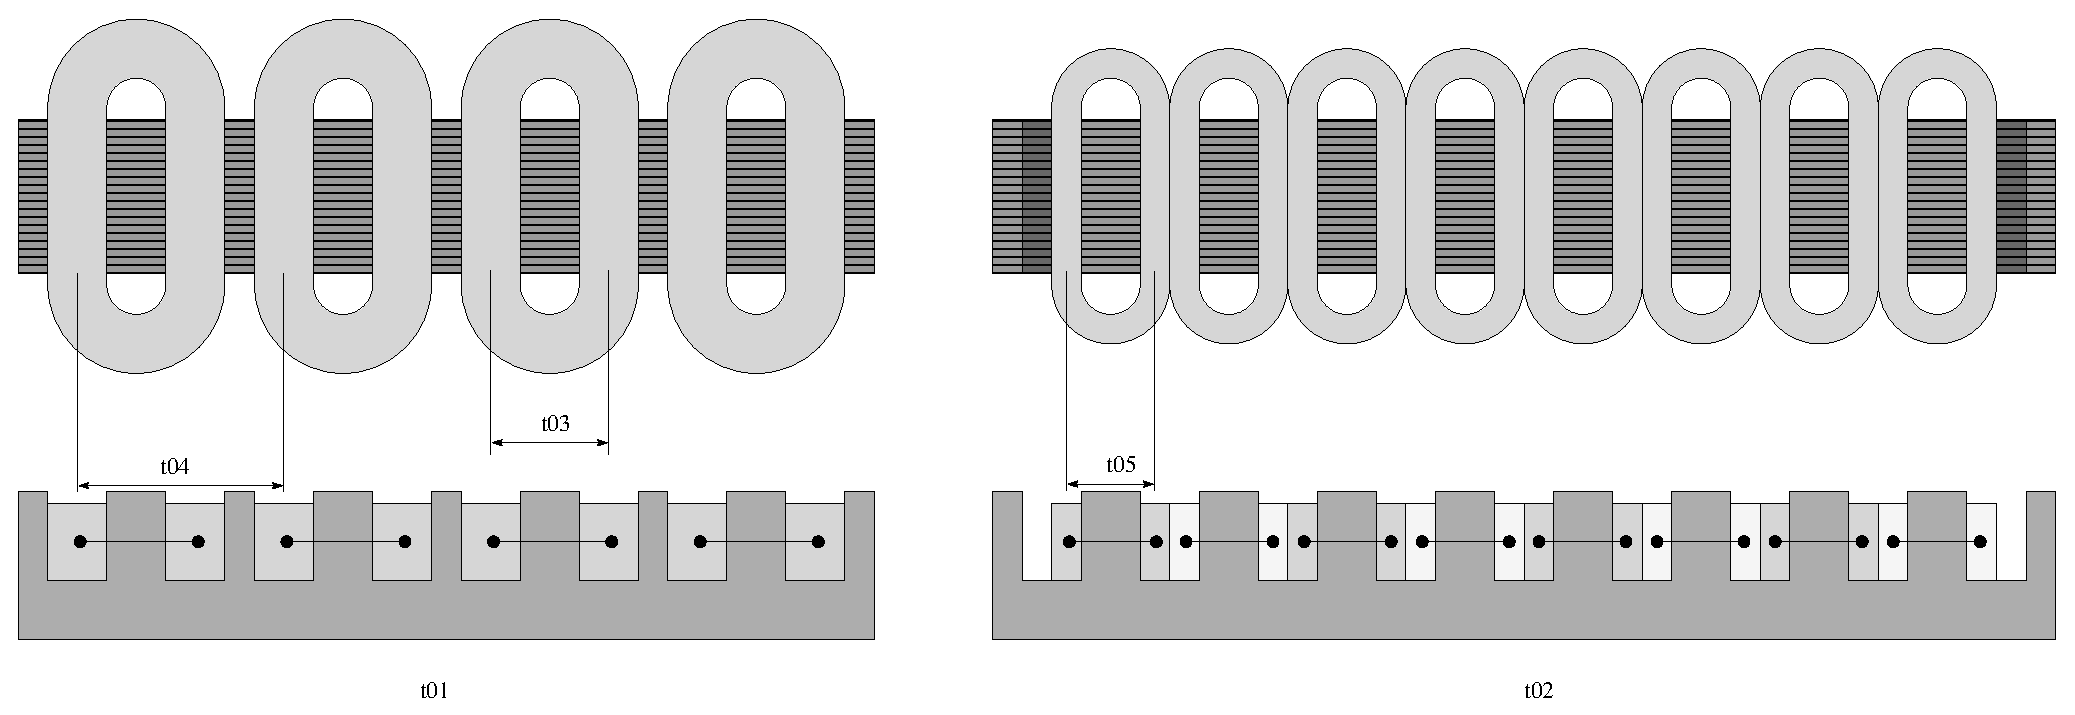
\includegraphics[width=1.00\textwidth]{figs/f_concen_coils.eps}
\end{psfrags}%
	\caption{Double and single layer non-overlapping windings}
	\label{fig:concen_coils}
\end{figure}

In the literature different definitions of terms are in use for non-overlapping concentrated windings. The most common of them are:
\begin{itemize*}
	\item \cite{IR-EE-EME_2003:029}: concentrated windings;
	\item \cite{IR-EE-EME_2004:022}: concentrated fractional pitch windings; 
	\item \cite{salminen_2004_ICEM}: fractional slot wound; and
	\item \cite{bianchi_2004}: fractional slot. 
\end{itemize*}

If the coils are to be equally in shape, which simplifies manufacturing, it is recognised that a single layer could easily have a variable slot pitch\footnote{The concept of a variable coil pitch is explained in chapter \ref{chap:DesignWindings}. Also refer to Fig.~\ref{fig:f_slotstar} for regular and irregular distributed slots.}. Furthermore, the coils could be implemented as either form-wound or round-wound. Returning to the variable coil pitch of the single layer, it is important to mention that this is an extra degree of freedom that offers to be an attractive design parameter. The air gap flux that links the coil could thus be increased and torque ripple can be improved. 

It is therefore helpful to classify a concentrated winding either as an overlapping or non-overlapping concentrated winding. \cite{cros_2002} certainly aroused interest in non-overlapping concentrated windings with their paper entitled ``Synthesis of High Performance PM Motors With Concentrated Windings'', since this is a paper which is very often used as a reference on these winding types. This could be a possible explanation for the use of the term ``concentrated windings'' rather than ``tooth coil windings''.

The expansion of the classical winding types used in machines by non-overlapping windings offers new possibilities in especially traction machine design. The main research question in section \ref{sec:problem_statement} suggests a design algorithm that takes into account the non-overlapping type. Obviously a method that is valid for all types is required. In addition, it should be easy to integrate into whichever process is in use. 

\section{Approach to the problem}
As a first step towards the analysis of interior permanent magnet synchronous machines with non-overlapping concentrated windings, an in depth overview of the systematics of $m$-phase windings is required. The paper of \cite{Kauders1932} and the book of \cite{Nuernerg1952} are two very good examples\footnote{This literature is unfortunately written in German, which means that it is not easily accessible for those with little or no German knowledge.}. A historical overview of winding design and tendencies in machine analyses are given in chapter \ref{chap:overview}.  

Addressing the research questions in section \ref{sec:problem_statement}, a good starting point would be to derive the air gap mmf using the classical single coil approach and then expand it for three phases. It would be ideal to find a systematic algorithm for assigning the coils to the stator slots. The derivation of the air gap mmf and winding theory is presented in chapter \ref{chap:DesignWindings}.

The new perspective on the winding representation and its properties offered in the present dissertation are then applied to a traction machine case study. Here only the degree of freedom that single layer non-overlapping windings provide, is focused on. This is explained in chapter \ref{chap:design}. Some important remarks on non-linear machine analysis to support the design results are explained in chapter \ref{chap:NonlinearAnalysis}.

A prototype and its measured results to verify the design process are given in section \ref{sec:prototype}. Finally, the conclusions and recommendations for further studies are presented in chapter \ref{chap:ConlusionsRecommendations}. 


\section{Scientific contributions of this dissertation}
The design of permanent magnet motors often results in the use of a fractional slot winding. Different methods are available to design these windings (which are often graphically presented), of which none takes into account single layer non-overlapping windings (which could have a variable slot pitch). Moreover, due to the different slot configurations, material non-linearities and saturation effects, it is impossible to find analytical methods to fulfill these requirements. In an everyday design environment it is necessary to have accurate and reliable tools. The scientific contribution of this dissertation can be summarised as follows:
\begin{itemize}
	\item A general method to design single layer non-overlapping windings with a 
	fixed and variable slot pitch is offered. The winding design is presented 
	in its most compact form and has all the information on the physical layout as 
	well as the winding harmonics. It will be shown that the developed method applies
	to $m$-phase windings in general as well.
	\item Developing an analytical model for the magnetic circuit of interior 
	permanent magnet motors is nearly impossible. A better method is to make use of 
	both the analytical and finite element method. The machine is characterised by 
	three (finite element analysis generated) two-dimensional functions and frequency
	dependent losses are calculated analytically.
	\item The methodology from the study is applied to a \SI{150}{kW} prototype motor 
	designed for a traction application. The manufactured machine has \num{30} stator
	slots and \num{20} poles. Practical measurements were done to verify the computational
	results presented.   
\end{itemize}	

\section{Delimitations of the study}
The aim of this study is the analysis of interior permanent magnet synchronous machines with single layer non-overlapping windings. A comparison with other machine types is not given. The single layer non-overlapping winding offers an inherent degree of freedom, namely the variable coil pitch. Since this is not typical for other\footnote{When referring to other winding types, it means double layer non-overlapping as well as single and double layer overlapping windings.} winding types, this will be the only design aspect that will be focused on. A detailed machine optimisation is not provided. 

\section{Layout of the dissertation}
The research results are presented in six chapters as follows:
\begin{description}
  \item[Chapter 2:] A short literature overview which gives a brief historical view~% 
  of winding design is presented. This is followed by general tendencies in machine~% 
  analyses.
	\item[Chapter 3:] An algorithm is derived to present a winding in a matrix~%
	form. This compact form allows the calculation of the winding factors for all~%
	harmonics. The basis of the algorithm is the phase belt sequence and the phase~%
	belt constraint which is derived from the air gap mmf envelope functions.
	\item[Chapter 4:] This chapter describes the nonlinear magnetic circuit analysis~%
	of the interior permanent magnet machine. The chosen method is that of the finite~%
	elements. The chapter starts off with an introduction to the nonlinear materials~%
	used in the design, followed by a detailed calculation of the relevant machine~%
	quantities which are necessary for a performance calculation.	The chapter concludes~%
	with a detailed explanation of how to perform a harmonic analysis.
	\item[Chapter 5:]  FEA
	and analytical methods are combined to introduce a design procedure suitable in an~%
	an everyday design environment. The chapter concludes with a case study of a~%
	prototype traction motor with non-overlapping single layer concentrated windings~%
	and interior permanent magnets. Practical measurements on the prototype are~%
	compared to calculated values and discussed.   
	\item[Chapter 6:] This chapter entails conclusion and recommendations for further study.
\end{description}
Where applicable all the explanations are accompanied by an example based on the prototype machine which has \num{30} stator slots and \num{20} poles. A detailed description for this combination is given in chapter \ref{chap:design}. 

\section{Difficulties encountered during the study} 
The major difficulty encountered during the study was the limitations of commercial finite element software to generate and post-process finite element analysis data in an efficient way. Even the integration thereof in customised software tools was nearly not possible. This difficulty was overcome by using non-commercial finite element software, FEMP (\textbf{F}inite \textbf{E}lement \textbf{M}ethod \textbf{P}rogram). However, it was first necessary (through intensive Fortran programming) to adapt the software to include permanent magnets and allow positive boundary conditions.

Initially the winding factor and results from the discrete Fourier transform were treated as absolute values. Keeping these values as complex numbers greatly simplifies the analysis, since (through a proper choice of reference axis) information on the winding axes and the $dq$-variables are given.    

\section{Notes to the reader}
The work presented in this thesis was done in N�rnberg, Germany. Consequently many of the literature used were in German. To name only a few, books by \cite{Nuernerg1952}, \cite{Klamt1962} and \cite{Jordan1975} are still commonly used in design offices. It is noticeable that even though there exists a list of symbols for various quantities, English and German have in some cases different symbols for the same quantity. This is mainly due to the fact that languages develop individual and of course colloquial language rules. Even a direct translation does not necessarily give the typical word used. An example is the German word \textit{Felderregerkurve}. A direct translation would be ``field excitation curve'', which of course is not wrong. However, the field excitation curve in electrical terms is usually known as the ``magnetomotive force'' (mmf). Tab.~\ref{tab:translation} gives some common electrical machine quantities in English and German, and the different symbols in use.
\begin{table}[htbp]
	\caption[Typical machine quantities and their German translation]%
	{Typical machine quantities, there German translation and~%
	counterpart symbols}
	\label{tab:translation}
	\centering
	\begin{tabular}{lccl}
	\toprule
	Quantity   &  English  & German & Unit \\
	\toprule
	magnetomotive force (\textit{Durchflutung}) & 
	$F$& $\Theta$ & \SI{}{A}\\
	\midrule
	flux linkage (\textit{Flussverkettung}) & 
	$\lambda$& $\psi$ & \SI{}{V.s}   \\
	\midrule
	voltage (\textit{Spannung})  & 
	$V$& $U$ & \SI{}{V} \\
	\midrule
	specific resistance (\textit{spezifischer Widerstand})&
	$\rho$& $\varrho$ & \SI{}{\ohm.m} \\
	\midrule
	specific weight (\textit{spezifischer Masse})&
	$\rho$& $\gamma$& \SI{}{kg.m^{-3}}\\
	\midrule
	conductivity (\textit{Leitf�higkeit})&
	$\sigma$&$\kappa$& \SI{}{S.m^{-1}}\\
	\midrule
	cross section area (\textit{Querschnitt})&
	$A$&$Q$& \SI{}{m^{2}}\\
	\midrule
	turn number (\textit{Windungszahl}) & 
	N& W & - \\
	\bottomrule
	\end{tabular}
\end{table}

It is commendable that the German terminology on electrical machines allows a very precise description of almost all aspects related to the subject. In many cases it is difficult to find an equivalent technical term in English, because it simply does not exist. The problem of different terminologies even exists within a language: different ``schools'' use different terms which makes the study of machine related books not easy. Also historical changes need to be kept in mind.

The term ``machine'' as used in the present dissertation means it could be a machine that is operated either as a motor or as a generator. In the title the term ``motor'' is used, since only the measured results of motor operation are presented. However, in the theoretical sections, the word ``machine'' is preferred.  

The document is optimised for a two-sided printout. A flip-book shows that the fundamental and fifth harmonic of the mmf rotate in the opposite direction.   




   




\chapter{Literature overview}\label{chap:overview}
In this chapter a brief overview of the history of stator windings (layout and design) is given. Since this topic evolved over many years an in depth history is beyond the scope of the present dissertation. However, a few important works need to be mentioned. 

\section{A historical view of winding design}
In the first of his two remarkable papers \cite{Kauders1932} explains the systematics of stator windings and the calculation of the winding factors. The aim in this work was to determine the parameters that characterise the air gap mmf of the winding. Also in this paper the induced voltage in the coil sides is already mentioned and represented as a vector. The resultant vector diagram was called the star of coil groups (German: ``Spulengruppenstern''). The adjacent vectors on such a diagram that belong to the same phase is called a phase belt (German: ``Zone'').

Two years later, in the second paper by \cite{Kauders1934}, the algebraic methods developed in the first paper were visualised by means of Tingley's diagram. The latter could be referred to as a linear representation of the now called star of slots (German: ``Nutenstern''). The star of slots is constructed using the electrical angle between two adjacent slots. Computer technology as we know it today was not available at the time and the use of graph paper certainly was common. Furthermore, such graphical methods definitely contributed to the subject of stator windings.

Vil\'em Kl\'ima (Wilhelm Kauders) died on 6 October 1985 and in an obituary by \cite{Frohne1985} it is mentioned that Kl\'ima's equation for the distribution factor\footnote{Also known as the breadth factor.} of fractional slot windings is not found in textbooks. Another remark in the obituary is that in some references it is stated that it is not possible to find a closed-form expression for the winding factor of fractional slot windings. In the rest of this literature overview, none of the authors (except Kremser) refers to or makes use of Kl\'ima's closed-form expression\footnote{A summary of closed-form expression is given in appendix \ref{app:klima}.}. 

More than fifty years later than \cite{Kauders1934}, \cite{Kremser1989} introduced a comprehensive study of fractional slot windings and the currents in the parallel paths of rotating machines. The reason for this big time gap does not mean that nothing had happened in the mean  time in winding design; it should be kept in mind that this overview only points out some important aspects. In the first part of Kremser's doctoral thesis a detailed algebraic description of single and double layer fractional slot windings is presented. In order to allocate the coils to the stator slots, modular arithmetic, which uses the so-called commutator pitch, is used. This can be seen as a step toward using computer programs to automatically performing winding designs. In the star of slots the vectors start wrapping, and once put on a graph, two vectors having angles of \ang{45} and \ang{405} respectively lie exactly on each other. The star of slots is thus the same as the remainder after dividing an angle by \ang{360} which can easily be implemented by means of the modulo function.     

\cite{Wach1997} explains another algebraic method to design stator windings which has much in common with that presented by \cite{Kremser1989}\footnote{It should however be noticed that the authors Wach and Kremser are from Poland and Germany respectively.}.  The methods presented in the paper is characterised by the matrix representation of a winding. The winding matrix simplify the winding factor calculation and avoids complex equations. Basically the vectors of the star of slots is used in matrix form. What is called the winding matrix could be seen as the matrix representation of Tingley's diagram. A drawback of the method is that each matrix entry for double layer windings has two values. In computer programming this should be solved by either a multi-dimensional matrix or two two-dimensional matrices. In another paper by \cite{Wach1998}, the focus is on the optimisation of fractional slot windings. In spite of the fact that this paper is a very good source on the topic of winding design, none of the literature in the rest of this section refers to it.
 
\cite{cros_2002} showed that the use of stator coils wound around the stator teeth has some attractive advantages for manufacturing. The coils do not overlap which means that the manufacturing is simplified and the winding overhang is less than that of overlapping windings. Electrically the shorter winding overhang means the use of less copper. Furthermore, the non-overlapping windings are derived from single or double layer overlapping windings. It is also pointed out that in the case of single layer non-overlapping windings the coil pitch can be increased and used as a design parameter\footnote{See Fig.~\ref{fig:f_slotstar} for regular and irregular distributed slots.}. The latter, however, is not taken into account in the winding factor calculation. This paper is referenced quite often, proving the interest among machine designers in non-overlapping windings.  

\cite{Salminen2004} did an extensive study on fractional slot windings for low speed applications. The main objective in the doctoral thesis is to compare different slot combinations of a machine with a fixed air gap diameter in the \SI{45}{kW} range. Although both single and double non-overlapping windings are taken into account, the focus is on the double layer type. Since round wire coils are used in the investigated application it is appropriate to use a double layer rather than single layer. If form-wound coils were used the choice of double layer windings would have caused some difficulties when inserting the coils into the stator slots. Also, the stator had semi-closed slots. The star of slots is referred to as the voltage vector graph in Salminen's thesis. A very important comment by the author is that care should be taken when the winding factors for different winding types are to be calculated. Depending on the winding type the right set of equations should be chosen. 

\cite{skaar_2006} proposed a method to calculate the winding factors for concentrated coils without knowledge of the winding layout. This is of course sufficient to quickly compare different slot and pole combinations. Using this method it is shown that the best number of slots per pole and phase should be in the range \textonequarter $\leq q\leq$ \textonehalf. 

The tutorial presented by \cite{Bianchi2007} is an in-depth study of fractional slot windings in general. In their tutorial notes a distinction is made between overlapping and non-overlapping windings. Here too the non-overlapping type is derived from a double layer overlapping winding. 

\section{Tendencies in machine analysis}
When analysing permanent magnet electrical machines it is not necessary to start from scratch. Since the induction machine has been known for more than \num{100} years the developed methods serve as a good basis. A well-known book on induction machines is \textit{Die Asynchronmaschine} (commonly known as the induction machine) by \cite{Nuernerg1952}. The book gives a very detailed description of modeling techniques which can be used in the design of induction machines (which is of course not limited to induction machines only). 

\subsection{Introductory remarks}
It is important to mention that \cite{Nuernerg1952} uses equivalent $B(H)$ curves for the calculation of the mmf's in the teeth and yoke. This is not wrong and indeed helps to understand the physical behaviour of the machine. However, the curves evolved over many years and are based on measured results and are only valid for steady-state operation. 

Fig.~\ref{fig:f_comp_teeth} illustrates the principle of leakage compensation (German: ``Zahnentlastung''). Due to saturation, flux lines leave the teeth tips and are parallel to the slot wall. This means that the flux density in the stator teeth decreases. Since the single layer non-overlapping winding could have a variable coil pitch the stator has two tooth types. The validity of the compensation curves given by \cite{Nuernerg1952} and applied to machines with different stator slots was not investigated and could be a very interesting topic for further study. The approach in the present dissertation is to use the finite element method, which calculates the exact flux densities by means of a physical model.
\begin{figure}[htbp]
	\centering
		\input{figs/ch2/f_comp_teeth.tex}
	\caption{Leakage compensation in the stator teeth}
	\label{fig:f_comp_teeth}
\end{figure}

\subsection{The finite element method as a design tool}
From most recent conference contributions there is a noticeable tendency to use numerical methods like the finite element method in the initial design phase. \cite{Germishuizen2007} proposed a new calculation method for calculating the machine performance from flux linkage and torque functions. These functions are obtained from a finite element analysis (FEA). 

\cite{Center2008} introduced a software tool for the design of high-speed induction machines. For such machines the loss calculation and the influence of the material properties are very important. Therefore, to account for these aspects the finite element method is combined with analytical expressions. \cite{Hafner2008} suggested a similar design strategy for the same reasons.

\cite{reichert_2_2004} explains a simplified approach to determine machine characteristics by means of the finite element method. In doing so the non-linear material behaviour is accounted for and is still fast and accurate. \cite{Garbe2008} also combines FEM and analytical expressions to calculate motor parameters.

\subsection{The influence of saturation on transient solutions}
\cite{seifert_1989} showed that the use of induction motor parameters calculated in the classical way leads to inaccurate predictions of machine behaviour under fault conditions such as terminal short circuits. Experienced based factors were introduced to account for the lack of accuracy. Again, this is an example of a situation where results must be known in order to obtain useful saturation factors.

Besides the saturation of the materials used the modeling thereof is also essential for machine behaviour. The material behaviour up to saturation is explained in section \ref{sec:mat_properties} and, where applicable, referenced to the literature. \cite{ponick_1993} showed that neglecting the effect of saturation in transient solutions can lead to inaccurate results. It is suggested that not only the inductances influenced by saturation, but the change in current as well, should be taken into account. Avoiding saturation could result in undersizing of critical mechanical components. Depending on the machine application, undersized mechanical parts can become a safety problem, for example in traction drives for rail vehicles.

\cite{retiere_1998} offered study methods of three-phase short circuits of induction machines. The reverse peak torque during a short circuit can cause serious mechanical stress. The authors show that for induction machines the saturation and the skin effect in the rotor bars should be accounted for in the calculation of the reverse peak torque and that it is necessary to take into account the saturation effects. \cite{Brauer2004a} compared the dynamic short circuits of induction machines (IM) to that of permanent magnet synchronous machines (PMSM). An important outcome of their study is that in the case of the two-phase short circuit a PMSM starts to oscillate and continues to do so until it is isolated from the inverter. It is also emphasised that these fault conditions should be calculated using FEM. \cite{Eichler2008} also describes that linear machine models cannot be used to simulate wind generators in the \SI{5}{MW} range.    

There is a lack of experience in the development of permanent magnet machines compared to induction machines. This means that the use of for example compensation curves to account for saturation should be avoided, since it might lead to inaccurate design calculations. Furthermore, it should be noticed that such compensation curves were developed also due to the lack of computation technology. At present the latter is no problem anymore and the use of state of the art technology is advisable for accurate predictions. This is even more important as prototyping (and measurements to find compensation factors) is to be kept to a minimum for economic reasons.  

\subsection{Normalised coefficients}
In times before the use of personal computers and calculators it was common to scale equations in such a way as to simplify mental arithmetic -- indeed one of those rare occurrences where a specific and easy to use number was chosen to simplify things \cite{REF-00716}. Books like \cite{REF-00004} and \cite{REF-00429} are two good examples where this is found. The two-term Jordan iron loss model is common in the following form:
\begin{equation}\label{eqn:pFe_norm}
  p\left(\frac{f}{f_n},\frac{J}{J_n}\right) = \left[\sigma_h\cfrac{f}{f_n}        + 
	           \sigma_c\left(\cfrac{f}{f_n}\right)^2\right] \cdot 
       \left(\cfrac{J}{J_n}\right)^2
  \qquad
  \begin{cases}
    \sigma_h = J_n^2 f_n k_h         \\
    \sigma_c = (J_nf_n)^2k_c   
  \end{cases}
\end{equation}
means that the coefficients will have different units\footnote{There are different software packages available to calculate the iron loss in electrical machines. Some packages require the $k$-coefficients while other packages make use of the $\sigma$-coefficients in \eqref{eqn:pFe_norm}. The coefficients $k_h$ and $k_c$ have the units \SI{}{W.kg^{-1}.f^{-1}.T^{-2}} and \SI{}{W.kg^{-1}.f^{-2}.T^{-2}} respectively -- \cite{REF-00012}. Using \eqref{eqn:pFe_norm} it will be \SI{}{W.kg^{-1}} for both $\sigma_h$ and $\sigma_c$.}. It is important to mention that the choice of $f_n$ and $J_n$ are arbitrary\footnote{At present $f_n=\SI{50}{Hz}$ and $J_n=\SI{1.5}{T}$ are typical. However, $J_n=\SI{1}{T}$ is also found in many (older) books dealing with iron losses.}. The basic principle is visually shown in Fig.~\ref{fig:M330-50A}\subref{fig:Measured} and Fig.~\ref{fig:M330-50A}\subref{fig:Calculated} for the measured and calculated (using a mathematical model) loss respectively. 
\begin{figure}[htbp]
  \centering
  \fontsize{8}{10}\selectfont
  \setlength\fwidth{0.4\textwidth}
  \subfloat[M330-50A\label{fig:Measured}]{
  % This file was created by matlab2tikz.
%
%The latest updates can be retrieved from
%  http://www.mathworks.com/matlabcentral/fileexchange/22022-matlab2tikz-matlab2tikz
%where you can also make suggestions and rate matlab2tikz.
%
\begin{tikzpicture}

\begin{axis}[%
width=0.951\fwidth,
height=0.75\fwidth,
at={(0\fwidth,0\fwidth)},
scale only axis,
every outer x axis line/.append style={black},
every x tick label/.append style={font=\color{black}},
xmin=0,
xmax=2,
xtick={0,1,2},
tick align=outside,
xlabel={$J/\SI{}{T}$},
xmajorgrids,
every outer y axis line/.append style={black},
every y tick label/.append style={font=\color{black}},
ymin=50,
ymax=200,
ytick={50,100,200},
ylabel={$f / \SI{}{Hz}$},
ymajorgrids,
every outer z axis line/.append style={black},
every z tick label/.append style={font=\color{black}},
zmin=0,
zmax=30,
zlabel={$p / \SI{}{W.kg^{-1}}$},
zmajorgrids,
view={322.5}{30},
axis background/.style={fill=white},
axis x line*=bottom,
axis y line*=left,
axis z line*=left,
legend style={at={(0.03,0.97)},anchor=north west,legend cell align=left,align=left,draw=black}
]
\addplot3 [color=blue,only marks,mark=+,mark options={solid}]
 table[row sep=crcr] {%
0.1	50	0.023\\
0.15	50	0.052\\
0.2	50	0.09\\
0.25	50	0.136\\
0.3	50	0.186\\
0.35	50	0.242\\
0.4	50	0.304\\
0.5	50	0.438\\
0.6	50	0.59\\
0.7	50	0.758\\
0.8	50	0.944\\
0.9	50	1.148\\
1	50	1.375\\
1.1	50	1.626\\
1.2	50	1.909\\
1.3	50	2.239\\
1.4	50	2.644\\
1.5	50	3.135\\
1.6	50	3.65\\
1.7	50	4.135\\
1.75	50	4.343\\
1.8	50	4.66\\
0.1	100	0.054\\
0.15	100	0.122\\
0.2	100	0.212\\
0.25	100	0.319\\
0.3	100	0.44\\
0.35	100	0.575\\
0.4	100	0.724\\
0.5	100	1.057\\
0.6	100	1.437\\
0.7	100	1.865\\
0.8	100	2.347\\
0.9	100	2.887\\
1	100	3.49\\
1.1	100	4.164\\
1.2	100	4.927\\
1.3	100	5.794\\
1.4	100	6.819\\
1.5	100	8.064\\
1.6	100	9.438\\
1.7	100	10.789\\
1.75	100	11.461\\
0.1	200	0.135\\
0.15	200	0.308\\
0.2	200	0.534\\
0.25	200	0.806\\
0.3	200	1.118\\
0.35	200	1.469\\
0.4	200	1.855\\
0.5	200	2.741\\
0.6	200	3.758\\
0.7	200	4.952\\
0.8	200	6.32\\
0.9	200	7.892\\
1	200	9.673\\
1.1	200	11.704\\
1.2	200	13.992\\
1.3	200	16.567\\
1.4	200	19.48\\
1.5	200	23.114\\
1.6	200	27.316\\
};
 \addlegendentry{data sheet};

\addplot3 [color=black!50!green,only marks,mark=o,mark options={solid}]
 table[row sep=crcr] {%
0.1	50	0.0143688192607135\\
0.15	50	0.0323298433366053\\
0.2	50	0.0574752770428538\\
0.25	50	0.0898051203794591\\
0.3	50	0.129319373346421\\
0.35	50	0.17601803594374\\
0.4	50	0.229901108171415\\
0.5	50	0.359220481517836\\
0.6	50	0.517277493385684\\
0.7	50	0.704072143774959\\
0.8	50	0.919604432685661\\
0.9	50	1.16387436011779\\
1	50	1.43688192607135\\
1.1	50	1.73862713054633\\
1.2	50	2.06910997354274\\
1.3	50	2.42833045506057\\
1.4	50	2.81628857509984\\
1.5	50	3.23298433366053\\
1.6	50	3.67841773074264\\
1.7	50	4.15258876634619\\
1.75	50	4.40045089859349\\
1.8	50	4.65549744047116\\
0.1	100	0.0360846656579069\\
0.15	100	0.0811904977302905\\
0.2	100	0.144338662631628\\
0.25	100	0.225529160361918\\
0.3	100	0.324761990921162\\
0.35	100	0.442037154309359\\
0.4	100	0.57735465052651\\
0.5	100	0.902116641447672\\
0.6	100	1.29904796368465\\
0.7	100	1.76814861723744\\
0.8	100	2.30941860210604\\
0.9	100	2.92285791829046\\
1	100	3.60846656579069\\
1.1	100	4.36624454460673\\
1.2	100	5.19619185473859\\
1.3	100	6.09830849618627\\
1.4	100	7.07259446894975\\
1.5	100	8.11904977302905\\
1.6	100	9.23767440842417\\
1.7	100	10.4284683751351\\
1.75	100	11.050928857734\\
0.1	200	0.101557439861734\\
0.15	200	0.228504239688901\\
0.2	200	0.406229759446935\\
0.25	200	0.634733999135836\\
0.3	200	0.914016958755604\\
0.35	200	1.24407863830624\\
0.4	200	1.62491903778774\\
0.5	200	2.53893599654334\\
0.6	200	3.65606783502241\\
0.7	200	4.97631455322495\\
0.8	200	6.49967615115096\\
0.9	200	8.22615262880043\\
1	200	10.1557439861734\\
1.1	200	12.2884502232698\\
1.2	200	14.6242713400897\\
1.3	200	17.163207336633\\
1.4	200	19.9052582128998\\
1.5	200	22.8504239688901\\
1.6	200	25.9987046046038\\
};
 \addlegendentry{estimation};

\end{axis}
\end{tikzpicture}%}
  \hfill  
  \subfloat[Normalised\label{fig:Calculated}]{
  % This file was created by matlab2tikz.
%
%The latest updates can be retrieved from
%  http://www.mathworks.com/matlabcentral/fileexchange/22022-matlab2tikz-matlab2tikz
%where you can also make suggestions and rate matlab2tikz.
%
\begin{tikzpicture}

\begin{axis}[%
width=0.951\fwidth,
height=0.75\fwidth,
at={(0\fwidth,0\fwidth)},
scale only axis,
every outer x axis line/.append style={black},
every x tick label/.append style={font=\color{black}},
xmin=0,
xmax=1.5,
tick align=outside,
xlabel={$\left.J/J_n\right|_{J_n=\SI{1.5}{T}}$},
xmajorgrids,
every outer y axis line/.append style={black},
every y tick label/.append style={font=\color{black}},
ymin=1,
ymax=4,
ytick={1,2,4},
ylabel={$\left.f / f_n\right|_{f_n=\SI{50}{Hz}}$},
ymajorgrids,
every outer z axis line/.append style={black},
every z tick label/.append style={font=\color{black}},
zmin=0,
zmax=30,
zlabel={$p / \SI{}{W.kg^{-1}}$},
zmajorgrids,
view={322.5}{30},
axis background/.style={fill=white},
axis x line*=bottom,
axis y line*=left,
axis z line*=left,
legend style={at={(0.03,0.97)},anchor=north west,legend cell align=left,align=left,draw=black}
]
\addplot3 [color=blue,only marks,mark=+,mark options={solid}]
 table[row sep=crcr] {%
0.0666666666666667	1	0.023\\
0.1	1	0.052\\
0.133333333333333	1	0.09\\
0.166666666666667	1	0.136\\
0.2	1	0.186\\
0.233333333333333	1	0.242\\
0.266666666666667	1	0.304\\
0.333333333333333	1	0.438\\
0.4	1	0.59\\
0.466666666666667	1	0.758\\
0.533333333333333	1	0.944\\
0.6	1	1.148\\
0.666666666666667	1	1.375\\
0.733333333333333	1	1.626\\
0.8	1	1.909\\
0.866666666666667	1	2.239\\
0.933333333333333	1	2.644\\
1	1	3.135\\
1.06666666666667	1	3.65\\
1.13333333333333	1	4.135\\
1.16666666666667	1	4.343\\
1.2	1	4.66\\
0.0666666666666667	2	0.054\\
0.1	2	0.122\\
0.133333333333333	2	0.212\\
0.166666666666667	2	0.319\\
0.2	2	0.44\\
0.233333333333333	2	0.575\\
0.266666666666667	2	0.724\\
0.333333333333333	2	1.057\\
0.4	2	1.437\\
0.466666666666667	2	1.865\\
0.533333333333333	2	2.347\\
0.6	2	2.887\\
0.666666666666667	2	3.49\\
0.733333333333333	2	4.164\\
0.8	2	4.927\\
0.866666666666667	2	5.794\\
0.933333333333333	2	6.819\\
1	2	8.064\\
1.06666666666667	2	9.438\\
1.13333333333333	2	10.789\\
1.16666666666667	2	11.461\\
0.0666666666666667	4	0.135\\
0.1	4	0.308\\
0.133333333333333	4	0.534\\
0.166666666666667	4	0.806\\
0.2	4	1.118\\
0.233333333333333	4	1.469\\
0.266666666666667	4	1.855\\
0.333333333333333	4	2.741\\
0.4	4	3.758\\
0.466666666666667	4	4.952\\
0.533333333333333	4	6.32\\
0.6	4	7.892\\
0.666666666666667	4	9.673\\
0.733333333333333	4	11.704\\
0.8	4	13.992\\
0.866666666666667	4	16.567\\
0.933333333333333	4	19.48\\
1	4	23.114\\
1.06666666666667	4	27.316\\
};
 \addlegendentry{data sheet};

\addplot3 [color=black!50!green,only marks,mark=o,mark options={solid}]
 table[row sep=crcr] {%
0.0666666666666667	1	0.0143688192607135\\
0.1	1	0.0323298433366053\\
0.133333333333333	1	0.0574752770428538\\
0.166666666666667	1	0.0898051203794591\\
0.2	1	0.129319373346421\\
0.233333333333333	1	0.17601803594374\\
0.266666666666667	1	0.229901108171415\\
0.333333333333333	1	0.359220481517836\\
0.4	1	0.517277493385684\\
0.466666666666667	1	0.704072143774959\\
0.533333333333333	1	0.919604432685661\\
0.6	1	1.16387436011779\\
0.666666666666667	1	1.43688192607135\\
0.733333333333333	1	1.73862713054633\\
0.8	1	2.06910997354274\\
0.866666666666667	1	2.42833045506057\\
0.933333333333333	1	2.81628857509984\\
1	1	3.23298433366053\\
1.06666666666667	1	3.67841773074264\\
1.13333333333333	1	4.15258876634619\\
1.16666666666667	1	4.40045089859349\\
1.2	1	4.65549744047116\\
0.0666666666666667	2	0.0360846656579069\\
0.1	2	0.0811904977302905\\
0.133333333333333	2	0.144338662631628\\
0.166666666666667	2	0.225529160361918\\
0.2	2	0.324761990921162\\
0.233333333333333	2	0.442037154309359\\
0.266666666666667	2	0.57735465052651\\
0.333333333333333	2	0.902116641447672\\
0.4	2	1.29904796368465\\
0.466666666666667	2	1.76814861723744\\
0.533333333333333	2	2.30941860210604\\
0.6	2	2.92285791829046\\
0.666666666666667	2	3.60846656579069\\
0.733333333333333	2	4.36624454460673\\
0.8	2	5.19619185473859\\
0.866666666666667	2	6.09830849618627\\
0.933333333333333	2	7.07259446894975\\
1	2	8.11904977302905\\
1.06666666666667	2	9.23767440842417\\
1.13333333333333	2	10.4284683751351\\
1.16666666666667	2	11.050928857734\\
0.0666666666666667	4	0.101557439861734\\
0.1	4	0.228504239688901\\
0.133333333333333	4	0.406229759446935\\
0.166666666666667	4	0.634733999135836\\
0.2	4	0.914016958755604\\
0.233333333333333	4	1.24407863830624\\
0.266666666666667	4	1.62491903778774\\
0.333333333333333	4	2.53893599654334\\
0.4	4	3.65606783502241\\
0.466666666666667	4	4.97631455322495\\
0.533333333333333	4	6.49967615115096\\
0.6	4	8.22615262880043\\
0.666666666666667	4	10.1557439861734\\
0.733333333333333	4	12.2884502232698\\
0.8	4	14.6242713400897\\
0.866666666666667	4	17.163207336633\\
0.933333333333333	4	19.9052582128998\\
1	4	22.8504239688901\\
1.06666666666667	4	25.9987046046038\\
};
 \addlegendentry{estimation};

\end{axis}
\end{tikzpicture}%}
  \caption{Measured and estimated specific loss} 
  \label{fig:M330-50A}
\end{figure}

\subsection{Present approaches in iron loss calculation}
The huge number of scientific contributions found on iron loss calculations emphasises the complexity of iron losses. Two aspects that definitely contribute to this fact is that the material data cannot be described analytically and is usually presented in graphical form. Secondly, the influence of the manufacturing process is difficult to account for. 

It is important to mention that a good approximation of the specific loss is found in \cite{Nuernerg1952}. Here the specific loss of one kilogram of deburred laminated steel in \SI{}{W} is given by
\begin{equation}
  \label{eqn:pfe_1}
  p_{Fe}= \left(k_h f+k_c f^2 \right) B ^2
\end{equation} 
The coefficients $k_h$ and $k_c$ account for the hysteresis and classical eddy current losses respectively. Since the frequency in the stator is constant for a given operating point it is convenient to separate the frequency and flux density components of the loss as in \eqref{eqn:pfe_1}. In N�rnberg's book it is also mentioned that the iron loss calculated in this way is less than the measured loss using the Epstein frame. To account for this inaccuracy it is suggested to multiply the calculated iron loss in the yoke and teeth by \num{1.5} and \num{3} respectively. This holds for stator slots which is semi-closed. For open stator slots the loss in the teeth tends to increase even further. Due to this uncertainty it is understandable that \cite{Nuernerg1952} advised the following\footnote{English: Due to the uncertainty in the iron loss calculation a detailed discussion is not given.}: ``Wegen der erheblichen Unsicherheit bei der Eisenverlustberechnung gehe man aber nicht in die Feinheiten.'' This shows the limits of empirical models before techniques like the finite element method were introduced. 

\cite{bertotti_1988} introduced what is called the excess loss and thereby expanded the analytical expression for specific loss by a $k_e (fB)^{1.5}$ term. Thus, \eqref{eqn:pfe_1} changes to    
\begin{equation}
  \label{eqn:pfe_2}
  p_{Fe}= \left(k_h f +k_c f^2 \right) B^2 + k_e (fB)^{1.5}
\end{equation} 
\cite{lin_2004} used the expression \eqref{eqn:pfe_2} in a transient finite element analysis. The advantage in doing so is that the actual flux densities are directly obtained from the finite element solution. \cite{Germishuizen2008} showed that the loss calculation in \eqref{eqn:pfe_2} is only a theoretical loss estimation based on extrapolated data obtained from results measured in the Epstein frame. Instead of using different factors for the yoke and teeth to account for the manufacturing influence, a single manufacturing factor should be applied to the overall result. For machines in the \SI{200}{kW} range a manufacturing factor of two is found to be adequate. Another outcome of this paper is that inadequate loss computations could easily lead to misinterpretation of results. 

\section[A short excursion]{A short excursion into the life of one of the authors consulted}\label{sec:excursion}
At this point I would like to make a short excursion and report a very interesting incidence for the following reasons:
\begin{itemize*}
	\item Nearly none of the references consulted took note of Vil\'em Kl\'ima's~%
	closed expression for the calculation of the distribution factor.
	\item Vil\'em Kl\'ima's life story is an inspiration for young researchers.
	\item Published research about the intellectual life of the Jewish elite in the~%
	ghetto Theresienstadt led me to this discovery.
\end{itemize*}
If one takes a closer look at the references listed in the last paper by  \cite{Klima1979}, there is an entry entitled \textit{Systematik der Drehstromwicklungen} and the author is given as V.~Kl\'ima (Kauders). To supply a name between brackets is not typical, and this occurrence made me suspicious, since the only paper I could find with this title is written by Wilhelm Kauders. As I could not explain the enigma, I started to ask questions and never expected to find answers about tragic events that occurred during the Second World War. Since I grew up in South Africa which, compared to other countries, was little effected by the war, this discovery made the experience extraordinary.    

\subsection{Coming across a very interesting source}
Nowadays it is typical to use the well-known Google search engine. Trying a few combinations of the names Kauders and Kl\'ima, I came across a list of lecturers in the ghetto of Terezin (Theresienstadt). The entry details for Kauders are given in Tab.~\ref{tab:EntryDetailsForKauders}.
\begin{table}[htbp]
	\caption{Kl\'ima's entry in the list of lecturers in the ghetto Theresienstadt}
	\label{tab:EntryDetailsForKauders}
	\centering
	\begin{tabular}{p{4.5cm}@{\hspace{22mm}}p{5.5cm}}
		\toprule
		Name and Title        & Kauders (Klima) (Vilem) Dr. \\\midrule
    Birth Date            & 10.04.1906                  \\\midrule
    Deported to Terezin   & 04.12.41                    \\\midrule 
    Deported from 	      & Prague \\\midrule
    Deported from Terezin & 01.11.44\\\midrule
    Survived in           & Grossrosen\\
    \bottomrule
	\end{tabular}
\end{table}
 
This led me to the book \textit{University Over The Abyss: The story behind 520 lecturers and 2,430 lectures in KZ Theresienstadt 1942-1944} by \cite{Makarova2004}. A very interesting detail from the book is that Dr.~Goldschmied and Dr.~Kauders were secretly taken to Germany to improve the performance of German radar\footnote{According to Ivan Kl\'ima (Kl\'ima's son), Vil\'em Kl\'ima was sent together with two other specialists: Mr. Goldschmied and Mr. Kohn to the concentration camp in Grossrosen. Mr.~Goldschmied and Kl\'ima stayed only for a few weeks in Grossrosen. As a result of the evacuation of the camp both of them were sent to KZ Sachsenhausen.}. A witness, Gerda Haas, remembered the following: 
\begin{quote}
``\textit{One day, the two were ordered to prepare themselves to leave Terezin. Their suitcases must have been cleaned of any signs and numbers, yellow stars were torn off. They were told that they would be employed for a large industrial concern in Germany. Their dependents stayed in Terezin. Soon, Kauders sent a postcard saying that he was in the [concentration camp] Rosenberg (or -burg), where he was freezing terribly and where he worked on his books all day.}''
\end{quote} 

The first book by Kl\'ima entitled \textit{Trojf\'azov\'e komut\'atorov\'e deriva\`en\'i motory: jejich teorie a praxe} was published in 1962. Then in 1975, together with H.~Jordan and K.P.~Kov\'acs, Vil\'em Kl\'ima published a book on induction machines entitled \textit{Asynchronmaschinen}. 

Through information supplied in the preface of the book published in 1975, I realised that Kl\'ima must have had contact with the University of Hanover, Germany. In this way I made contact with Prof.~Hans Otto Seinsch at the same university who kindly provided me with details on Kl\'ima and even gave me the contact details of one of Kl\'ima's students, Prof.~Zden\u{e}k \v{C}e\v{r}ovsk\'y. Since Prof.~\v{C}e\v{r}ovsk\'y was not only a student of Kl\'ima, but also a friend, I managed to contact Kl\'ima's son, Ivan Kl\'ima. 

An obituary in German was written by \cite{Frohne1985} and one in Czech by \cite{Cevrovsky1986}.

\subsection{A short biography of Vil\'em Kl\'ima}
Vil\'em Kl\'ima finished his studies with distinction in 1928 at the German technical University in Prague. He then started to work for the company \v{C}eskomoravsk\'a-Kolben-Dan\v{e}k (\v{C}KD) in Prague. In 1932 Vil\'em Kl\'ima received his \textit{Dr.-Ing.} for his dissertation entitled \textit{Systematik der Drehstromwicklungen}.

After the Munich Agreement in September 1938 the Czech boundary territory was occupied by the German army and later in March 1939 the whole of Czechoslovakia was occupied. Then, in November 1941, Vil\'em Kl\'ima was ordered to leave for the concentration camp at Terezin, which was a holding camp for Jews from central and southern Europe, and was regularly cleared of its overcrowded population by transports to death camps such as Auschwitz. During April 1944 Vil\'em Kl\'ima survived the so-called death march (a miracle at that time). Because of the hated German occupations of Czechoslovakia, Kl\'ima changed his name from Wilhelm Kauders to Vil\'em Kl\'ima. At the time it was a frequent decision of Czech families with German names to change their names to Czech-sounding names.  

After the war Kl\'ima started a research centre, \textit{Centre for Electric Machines}, in Brno where he was the first director until 1951. In 1958 Kl\'ima was awarded the title of ``Dr.Scientium technicarum'' for his thesis entitled \textit{Theorie der Selbstserregung von Drehstromnebenschlu�-kommutatormotoren mit Kondensatoren im L�uferkreis und ihre Verh�tung}. Until his retirement in 1973 he was part of the research centre in B\v{e}chovice near Prague. Vil\'em Kl\'ima died on 6 October 1985 in Prague.  

Taking note of the difficult circumstances Kl\'ima encountered during his life, any researcher in the field of electrical engineering can indeed feel inspired.         

\begin{figure}[h!]
	\centering
		\includegraphics[width=0.35\textwidth]{figs/ch2/Kauders.eps}
		\hfill
		\includegraphics[width=0.30\textwidth]{figs/ch2/Kauders_b.eps}
	\caption{Vil\'em Kl\'ima, 10.04.1906-06.10.1985}
	\label{fig:Kauders}
\end{figure}


\endinput

\chapter{Design and analysis of stator windings}
\label{chap:DesignWindings}
In order to answer the research sub-questions, this chapter is devoted to a derivation of an algorithmic method to design $m$-phase symmetrical windings and a representation thereof in a compact form. The basic principle of the winding of an electrical machine is to obtain a rotating magnetic field in the stator (the stationary part) that interacts with the moving part (the rotor). This is achieved by arranging the coils of the winding in the stator slots around the air gap periphery in such a way that a rotating field is developed when applying currents. As a result the induced voltage, which arises from flux per pole $\hat{\Phi}$, is obtained from Faraday's law. In general the sinusiodally induced voltage for a winding having $N_s$ series turns per phase is
\begin{equation}
  \label{eqn:ui}
  U_i = \sqrt{2} \pi f_1 \xi_p N_s \hat{\Phi}, \qquad \xi_p \leq 1
\end{equation}
where $\xi_p$ is the winding factor of the \textit{working harmonic}. The induced voltage in \eqref{eqn:ui} brings the importance of the winding design to the fore. For a given design requirement, it is desirable to have $\xi_p$ as high as possible.

\section{Definition of the working harmonic}\label{sec:working_harmonic}
Throughout the analysis all harmonics are referred to in terms of the bore $2\pi$ of the machine, i.e.~the \textit{fundamental harmonic} has the order $\nu=1$ and forms one pole pair. The harmonic that produces the magnetic field that interacts with the rotor poles $2p$ has the order $\nu=p$ and is called the \textit{working harmonic}. Any other harmonic of the $\nu^{th}$ order will have $\nu$ pole pairs and spans a peripheral angle of $\frac{2\pi}{\nu}$.

Often the harmonic orders are normalised with respect to the \textit{working harmonic}, i.e.~$\xi_{\nu /p}$. This then means that the \textit{working harmonic} is written as $\xi_1$ and sub-harmonics will have a fraction as subscript. This notation will not be used in the present dissertation.

\section{Classification of symmetrical windings}%
\label{sec:m_phases}
The winding design can be quite a difficult task and at this point it is useful to have a coarse classification of symmetrical windings. Since symmetrical windings comprise such a great variety, an attempt to categorise them will depend on the properties by which they are to be sorted. 

\subsection{Slots and coils per pole and phase} \label{subsec:slots_coils}
Any $m$-phase winding could be characterised by its number of slots per pole and phase. However, when comparing different winding designs with each other this number alone is insufficient. It does not take into account the number of layers the winding has. In addition, the number of coils per pole and phase should be defined. For a machine with $Q_s$ stator slots, $p$ pole pairs and $m$ phases the following definitions holds:
\begin{defth}
Slots per pole and phase: 
\begin{equation}
  q =\frac{Q_{s}}{m2p}=\frac{q_{n}}{q_{d}}
\end{equation}
$\frac{q_{n}}{q_{d}}$ is the reduced form of $q$. Each phase has $q_n$ slots that are distributed over $q_d$ poles. In the case where $q_d$ equals one, $q$ is an integer and the winding is called an integer slot winding. When $q_d$ is greater than one, it is called a fractional slot winding. 
\end{defth}
\begin{defth}
Coils per pole and phase: 
\begin{equation}
  q_{c}=\frac{Q_{c}}{m2p}=\frac{q_{c_n}}{q_{c_d}}
\end{equation}
$\frac{q_{c_n}}{q_{c_d}}$ is the reduced form of $q_c$. Each phase has $q_{c_n}$ coils distributed over $q_{c_d}$ poles. If $q_{c_n}$ is greater than one and $q_c$ is not equal to one it is a distributed winding. 
\end{defth}
These characteristic numbers give useful information on the winding when they are written as a reduced improper fraction\footnote{The reduced fraction could be either a proper or an improper fraction. An improper fraction has the numerator greater than the denominator.}. Additionally, the properties of single and double layer windings are summerised in Tab.~\ref{tab:properties_single_double}. 
\begin{table}[htbp]
	\caption{Properties of single and double layer windings}
	\label{tab:properties_single_double}
  \centering
  \begin{tabular}{p{3.5cm}@{\hspace{20mm}}p{3.5cm}}
  \toprule
	single layer winding & double layer winding \\
	\midrule
	$q = 2q_c$ & $q = q_c$ \\
	\midrule
	$Q_s = 2Q_c$ &  $Q_s = Q_c$ \\
	\bottomrule
	\end{tabular}
\end{table}

\subsection{Average coil pitch}
The coil pitch is defined as the peripheral angle between the two coil sides. It is practical to express the coil pitch in terms of the number of slots. Therefore, it is an integer number. 
\begin{defth}
The average coil pitch is defined as
\begin{equation}
  \label{eqn:y_p}
  y_p = \frac{Q_s}{2p}
\end{equation}
and the implemented coil pitch is given by
\begin{equation}
  \label{eqn:y_d}
  y_d = \mbox{int}(y_p)\pm k
  \quad
  \begin{cases}
    k \in \mathbb{N} \\
    y_d \geq 1
  \end{cases}
\end{equation}
\end{defth}
In the case where $y_d=y_p$ it is a full-pitch winding. If $y_d \neq y_p$ it is called a fractional pitch winding. 
 
\subsection{Classification scheme}
The aim of the classification scheme is to find a way to relate different winding types to each other. It is also a useful guideline to compare windings that belong to the same category. For the design methodology offered in the present dissertation, the following winding parameters are chosen for the classification:
\begin{enumerate*}
	\item the reduced form of the number of coils per pole per phase;
	\item the average coil pitch; and 
	\item the number of layers.
\end{enumerate*}
Fig.~\ref{fig:classification} shows a possible way to classify symmetrical $m$-phase windings. The reason for choosing the average coil pitch as a second property arises from the construction of the coils and it is valid for all types of windings. It could be seen as the ideal coil pitch. Additionally, the number of layers is a key parameter since the technology for manufacturing and the material used in single layer windings are different from that used in double layer windings. Using this classification scheme, the following definitions are associated with windings:
\begin{description}
	\item[Distributed winding:] If the numerator $q_{cn}$ of $q_c$ is greater than~%
	one, the winding is distributed. This means that the coil sides are distributed~%
	over $q_{cn}$ slots. The opposite of a distributed winding is a concentrated~%
	winding.
	\item[Concentrated winding:] In the case where $q_{c_n}$ equals one, it is called~%
	a concentrated winding. 
	\item[Concentrated coil:] When $y_d$ equals one, it is a concentrated coil. In~%
	this case the coil is concentrated around a stator tooth.
	a concentrated winding. 
	\item[Single and double layer:] These windings are differentiated by the number~%
	of coils compared to the number of stator slots. In single layer windings the~%
	number of coils equals half the number of stator slots, while for double layer~%
	windings the number of coils is equal to the number of stator slots. In the~%
	present dissertation a double layer winding has two coil sides per slot which could~%
	placed radially in two layers or side by side. 
	\item[Overlapping and non-overlapping:] In overlapping windings the coils overlap~%
	and the coil pitch $y_d$ is greater than one. If the coil pitch $y_d$ equals one,~%
	the coils do not overlap.
	\item[Integral slot winding:] If the denominator $q_d$ equals one, the phase~%
	belt has $q_n$ slots over one pole.
	\item[Fractional slot:] The denominator of $q$ is greater than one. This~%
	means that the $q_n$ slots are distributed over $q_d$ poles. In addition,~%
	the average coil pitch $y_p$ is a fraction. 
\end{description}
\begin{figure}[htbp]
	\centering
		\begin{psfrags}%
\psfragscanon

% text strings:
\psfrag{t01}[bc]{Symmetrical $m$-phase windings}
\psfrag{t02}[bc]{$%
                         q=\cfrac{Q_s}{m2p}=\cfrac{q_n}{q_d}%
                         \quad%
                         \mbox{and}%
                         \quad%
                         q_c=\cfrac{Q_c}{m2p}=\cfrac{q_{c_n}}{q_{c_d}}%
                        $}
\psfrag{t03}[bc]{Single layer}
\psfrag{t04}[bl]{$Q_c=\frac{1}{2}Q_s$}
\psfrag{t05}[bc]{Double layer}
\psfrag{t06}[br]{$Q_c=Q_s$}
\psfrag{t07}[bc]{Overlapping}
\psfrag{t08}[br]{$y_d>1$}
\psfrag{t09}[bc]{Non-overlapping}
\psfrag{t10}[bl]{$y_d=1$}
\psfrag{t11}[bc]{Overlapping}
\psfrag{t12}[bc]{$y_d>1$}
\psfrag{t13}[bc]{Non-overlapping}

\psfrag{t21}[bc]{$Q_c$}

\psfrag{t14}[bc]{$y_d$}
\psfrag{t15}[bc]{Full-pitch}
\psfrag{t16}[bl]{$y_d=y_p$}
\psfrag{t17}[bc]{Fractional pitch}
\psfrag{t18}[br]{$y_d \neq y_p$}

\psfrag{t28}[bl]{$q_d=1$}
\psfrag{t29}[bc]{$q_d$}
\psfrag{t30}[br]{$q_d>1$}
\psfrag{t31}[bc]{Integral slot}
\psfrag{t32}[bc]{Fractional slot}

\psfrag{t23}[bl]{$q_{c_n}=1$}
\psfrag{t24}[bc]{$q_{c_n}$}
\psfrag{t25}[br]{$q_{c_n}>1$}
\psfrag{t26}[bc]{Concentrated}
\psfrag{t27}[bc]{Distributed}

\psfrag{t33}[bc]{$y_p=\cfrac{Q_s}{2p}%
                    \quad%
                    \mbox{and}%
                    \quad%
                    y_d=\mbox{int}(y_p) \pm k%
                    \quad%
                    \begin{cases}%
                      k \in \mathbb{N}\\%
                      y_d \geq 1%
                    \end{cases}$
                  }

% Figure:
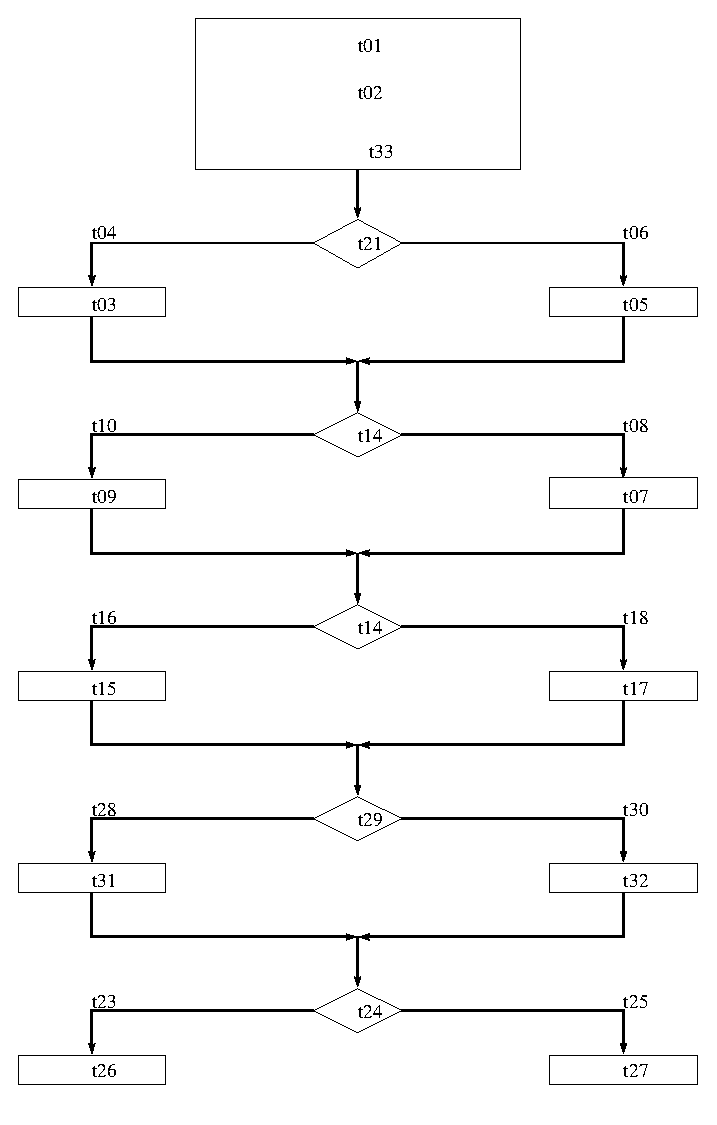
\includegraphics[width=0.8\textwidth]{figs/ch3/f_classification.eps}
\end{psfrags}%
  \caption{Classification of symmetrical $m$-phase windings}
	\label{fig:classification}
\end{figure} 

It is important to distinguish between a concentrated winding and a concentrated coil. The classification scheme in Fig.~\ref{fig:classification} defines a concentrated winding in a unique way. Concentrated windings are defined differently in literature. \cite{salminen_2004_IAS} refers to it as a traditional single layer winding whereas \cite{IR-EE-EME_2003:029} refers to it as distributed.

Particularly the windings defined as a fractional slot are very attractive for use in permanent magnet synchronous machines. Especially the single layer non-overlapping winding could be used to reduce
\begin{itemize*}
	\item manufacturing costs compared to overlapping windings;
	\item the end winding losses;
	\item torque ripple; and
	\item the mutual coupling between the phases.
\end{itemize*}

\section{Characteristics of symmetrical windings}
This section contains the major properties by which symmetrical $m$-phase windings are characterised.

\subsection{Basic winding}
\begin{defth}
The smallest repetitive segment is called the basic winding (German: ``Urwicklung'').
\end{defth} 
Due to symmetry only the basic winding needs to be determined. If $q_d$ is less than $p$ the winding is composed of $t$ identical \textit{basic windings}, i.e.
\begin{equation}
  \label{eqn:gcd_t}
  \begin{array}{ll}
  t = \begin{cases}
        \gcd\left(Q_s,p\right)  & \text{for double layer}\\
        \gcd\left(\frac{Q_s}{2},p\right) & \text{for single layer}
      \end{cases}
  \end{array}
\end{equation}
and gcd is called the greatest common divisor. In the case where $t=1$ the winding has no symmetry. Each of the $t$ \textit{basic windings} will have $Q_b$ slots and $p_b$ pole pairs, therefore
\begin{equation}
  \label{eqn:qd_pb}
  Q_b = \frac{Q_s}{t} \quad \mbox{and} \quad p_b = \frac{p}{t} 
\end{equation}
The number $p_b$ is the reduced pole pair. Another way of obtaining this number is by means of the denominator of $q_c$, i.e.
\begin{equation}
  \label{eqn:p_b}
  p_b =  
  \begin{cases}
    \frac{1}{2} q_{c_d}  & q_{c_d} \: \textnormal{even} \\
    q_{c_d}  & q_{c_d} \: \textnormal{odd}
  \end{cases}
\end{equation} 
which is independent of $t$. Examining \eqref{eqn:gcd_t}, it is recognised that $t$ can be rewritten as the gcd between the number of coils and the pole pairs, i.e.
\begin{equation}
  \label{eqn:gcd_t_gcd(Qc_p)}
  t = \gcd(Q_c,p) \quad
  \begin{cases}
    Q_c = Q_s \quad & \textnormal{double layer} \\
    Q_c = \frac{1}{2}Q_s \quad & \textnormal{single layer}
  \end{cases}
\end{equation} 
which is valid for both single and double layer windings. Although $t$ is usually used as a variable for time it is commonly found in literature and will be used in the same way throughout this chapter. Since the winding design is independent of time, it does not cause any confusion.

It is favourable to use the terms ``in and out going coil sides''\footnote{This is similar to the current which is defined as into and out of the page.}. Only the in going coil side needs to be assigned\footnote{The use of coil sides are preferred above coils, since it is then independent whether the coil sides belong to the same coil or not.} since the out going coil side is given by the coil pitch and type of winding.

\subsection{Winding symmetry}
For a winding to be symmetrical the number of coils used in each of the phases must be equal. Therefore the quotient between $Q_c$ and $m$ must be an integer. A requirement for a winding to be symmetrical can be derived from \eqref{eqn:qd_pb}. The symmetry condition can be expressed as
\begin{equation}
  \label{eqn:feasibility}
  \frac{Q_s}{t} = mk, \quad  k \in  \mathbb{N}
\end{equation}
which relates the pole number, number of stator slots and phase number to each other. A very useful function employed in the method is the modulo function which finds the remainder after division, i.e.~ $\textnormal{mod}(a,b)=a-\textnormal{floor}(\frac{a}{b})$\footnote{The floor function of a real number $x$, floor($x$), is a function whose value is the largest integer less than or equal to $x$.}. When using the modulo function it means that $\textnormal{mod}(\frac{Q_s}{t},m)$ must equal zero. There are different ways of deriving the constraints for the winding symmetry condition. Tab.~\ref{tab:feasibility} gives different variations found in the literature to express the symmetry condition. 
\begin{table}[h]
  \caption{Constraints for winding symmetry}
  \label{tab:feasibility}
  \centering
  \begin{tabular}{ll}
  \toprule %
  Reference & Constraint \\
  \toprule %
  \multirow{2}*{\cite{Wach1997}} & $\gcd(q_{c_d},m)=1$  \\\cmidrule {2-2}
  &$\mbox{mod}\bigl(\frac{Q_c}{q_{c_n}}q_{c_d},m\bigr)=0$\\\midrule   
  \cite{cros_2002} & $\mbox{mod}\bigl(\frac{Q_s}{\gcd(Q_s,2p)},m\bigr)=0$ 
  \\\midrule
  \cite{Bianchi2007} & $\mbox{mod}\bigl(\frac{Q_s}{t},m\bigr)=0$ 
  \\\bottomrule
  \end{tabular}
\end{table}

\subsection{Reduced number of pole pairs}
The lowest harmonic generated by a winding is given by $t=\gcd\left(Q_c,p\right)$ and the working harmonic equals $p$. The reduced pole number gives information on the subharmonics which are summarised as follows:
\begin{equation}	
 \begin{aligned}
	t &= p \quad \textnormal{the winding has no subharmonics} \\
	t &< p \quad \textnormal{the winding has subharmonics}
	\end{aligned}
\end{equation} 

The reduced number of pole pairs can be calculated in two different ways. Two greatest common divisors, i.e.~$\gcd\left(Q_c,2\,m\,p\right)$ and $\gcd\left(Q_c,p\right)$, are used to get $q_{c_d}$ and $p_b$ respectively. The relationship between these two factors is as follows:
\begin{equation}
  \label{eqn:reduced_p} 
  \gcd\left(Q_c,p\right)=\frac{\gcd\left(Q_c,2\,m\,p\right)}{r} \hspace{15pt}
  \textnormal{where} \hspace{15pt} r=
  \begin{cases}
	 m  & \text{$q_{c_d}$ even}\\
	 2m & \text{$q_{c_d}$ odd}
  \end{cases}
\end{equation}

\section{Rotating mmf}
Distributing the coils around the air gap periphery firstly requires the winding characteristic as explained in section \ref{subsec:slots_coils} and secondly a constraint assuring that the coils are assigned uniquely to the stator slots. Deriving such a constraint is done by means of the magnetomotive force (mmf) produced by a winding. 

In the theory of three-phase windings the rotating magnetic field is derived from a single coil with $N_t$-turns. The mmf produced by the coil is then written as a Fourier series which allows it to be decomposed in the \textit{working harmonic}, higher order harmonics and sub-harmonics if applicable. A detailed mathematical derivation is given by \cite{helle_1977}. It is also possible to explain the decomposition by means of visualisation as shown in \cite{Nuernerg1952}, \cite{Jordan1975} and  \cite{Fitzgerald1992}. The visualisation method is preferred and is used in the next sections in order to define the mmf envelope functions. This is necessary to answer the research sub-question which is the mathematical expression that defines a phase belt.

\subsection{The mmf of a single turn coil}%
\label{subsec:nt-turn_coil}
Consider a single coil with $N_t$-turns carrying a current $i$ placed in the stator of a machine with a uniform air gap as shown in Fig.~\ref{fig:mmf_1}(a). Assuming an infinite permeability in the laminated parts, the mmf in the stator and rotor can be neglected. This means the mmf across the air gap will be equal to the total mmf. 
 
\begin{figure}[htbp]
	\centering
		\begin{psfrags}%
\psfragscanon

% text strings:
\psfrag{x01}{$0$}
\psfrag{x02}{$\frac{\pi}{3}$}
\psfrag{x03}{$\frac{2\pi}{3}$}
\psfrag{x04}{$\pi$}
\psfrag{x05}{$\frac{4\pi}{3}$}
\psfrag{x06}{$\frac{5\pi}{3}$}
\psfrag{x07}{$2\pi$}

\psfrag{t01}{-1}
\psfrag{t02}{+1}
\psfrag{t03}{$C_2$}
\psfrag{t04}{$C_1$}
\psfrag{t05}{$F$}
\psfrag{t06}{$\frac{4}{\pi}\frac{N_ti}{2}\sum\limits_{\nu=1}^{\infty}
            \frac{1-(-1)^{\nu}}{2} \frac{1}{\nu}\cos(\nu \theta)$}
\psfrag{t07}[br]{$\theta$}
\psfrag{t08}{$\mu \rightarrow \infty$}
\psfrag{t09}{magnetic}
\psfrag{t10}{axis}
\psfrag{t11}{$p_1$}
\psfrag{t12}{$\theta^{+}$}
\psfrag{t13}{$\frac{4}{\pi}\frac{N_ti}{2}\cos \theta$}
\psfrag{t14}{current sheet}
\psfrag{t15}{$N_t i$}
\psfrag{t16}{$C_3$}
\psfrag{t17}{(a)}
\psfrag{t18}{(b)}
\psfrag{t19}{$\delta$}

% Figure:
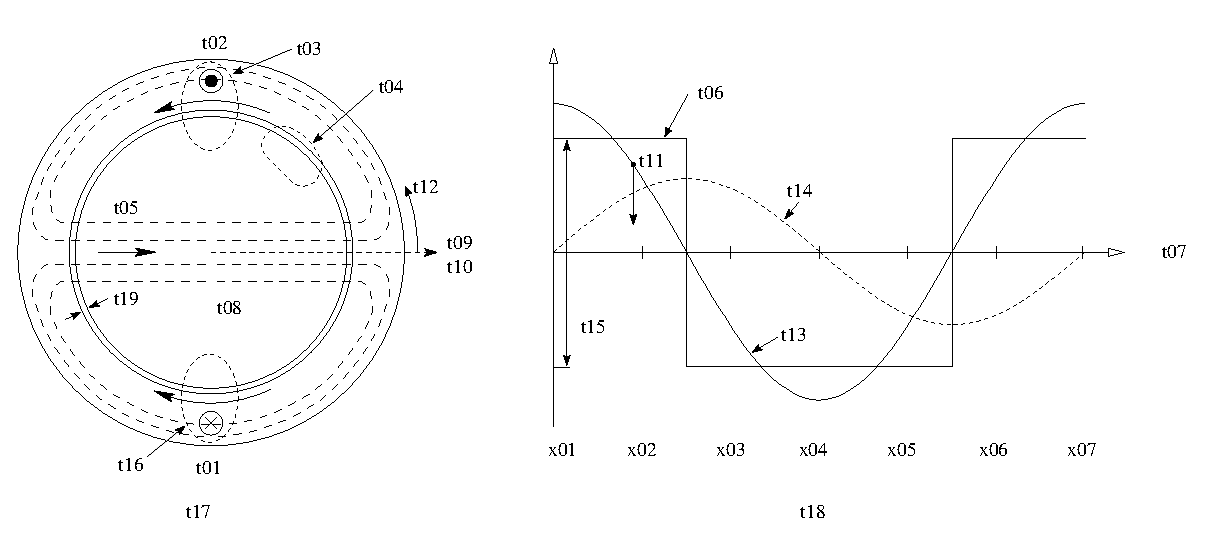
\includegraphics[width=1.00\textwidth]{figs/f_mmf_1.eps}
\end{psfrags}%
  \caption{Spatial mmf distribution for a $N_t$-turn coil}
  \label{fig:mmf_1}
\end{figure}

The spatial mmf distribution around the air gap periphery is obtained by applying Amp\`ere's law to the contours $C_1$, $C_2$ and $C_3$. The results of the integration are given in \eqref{eqn:int_H}. The integral along $C_1$ is zero since the contour does not enclose any source. Contrary to this the integrals along $C_2$ and $C_3$ equal $N_ti$ and $-N_ti$ respectively. The current in coil side $+1$ is positive, and using the right hand rule, out of the page.  
\begin{equation}
 \label{eqn:int_H}
 \oint \vec{H} \cdot d\vec{l}=
 \begin{cases}
   \begin{array}{llll}
     0  & C_1 & 0 \leq \theta < \frac{\pi}{2} 
     & \Rightarrow H(0)=H(\theta_1)\\
     N_ti & C_2 & \frac{\pi}{2} \leq \theta < \frac{3\pi}{2} 
     & \Rightarrow H(0)-H(\theta_2) = \frac{N_ti}{\delta} \\
     -N_ti & C_3 & \frac{3\pi}{2} \leq \theta < \frac{5\pi}{3} 
     & \Rightarrow H(0)-H(\theta_3) = \frac{N_ti}{\delta}
   \end{array}
 \end{cases}
\end{equation}
Since the flux to and from the rotor are equal, the air gap mmf will have an amplitude of $\frac{N_ti}{2}$. Fig.~\ref{fig:mmf_1}(b) shows the spatial of the single coil. This is a square wave and from the Fourier series the fundamental has an amplitude of $\frac{4}{\pi}$. The fundamental mmf can be seen as the result of a sinusoidally distributed current sheet on the stator inner diameter. When the coil is supplied by a current 
\begin{equation}
  i = \hat{I}\cos\omega t
\end{equation}
any point on the mmf will have a vertical trajectory. For example, the point $p_1$ will start moving downward for $t^+$ until it reaches a minimum from where it will start to move upwards again. Applying a sinusoidal current to the coil results in a standing wave in the air gap. The spatial mmf distribution has the form
\begin{equation}
  \label{eqn:F_theta_t_1}
  F(\theta,t) = \frac{4}{\pi}\frac{N_t }{2}\cos\theta \left(\hat{I}\cos \omega t\right)
\end{equation}
and will have nodes at $\frac{\pi}{2}$ and $\frac{3\pi}{2}$ while the anti-nodes will be at $0$ and $\pi$. Using a trigonometrical identity\footnote{$\cos A \cos B = \frac{1}{2}\cos(A-B)+\frac{1}{2}\cos(A+B)$} \eqref{eqn:F_theta_t_1} can be rewritten as the superposition of two rotating waves
\begin{equation}
  \label{eqn:F_theta_t_2}
  \begin{aligned}
  F(\theta,t) &= \frac{1}{2}\frac{4}{\pi}\frac{N_t }{2}\hat{I}\cos(\theta - \omega t)
  +\frac{1}{2}\frac{4}{\pi}\frac{N_t }{2}\hat{I}\cos(\theta + \omega t) \\
  &= F^+ + F^-
  \end{aligned}
\end{equation}
The result in \eqref{eqn:F_theta_t_2} means that a single coil produces two opposite rotating mmf waves in the air gap. In the next section this result is used to produce a single rotating mmf by displacing different coils in space. 

\subsection{The mmf of three single turn coils}
Producing a single rotating mmf wave using three coils means that each of the spatial mmf distribution functions must have a displacement for both the spatial and time component. Using \eqref{eqn:F_theta_t_2}, the resultant mmf for three coils will have the following form, i.e.
\begin{equation}
  \begin{aligned}
  F_R(\theta,t) &= (F_{1}^{+}+F_{1}^{-})+(F_{2}^{+}+F_{2}^{-})+(F_{3}^{+}+F_{3}^{-})\\
  &=(F_{1}^{+}+F_{2}^{+}+F_{3}^{+})+(F_{1}^{-}+F_{2}^{-}+F_{3}^{-})\\
  &=\sum_{n=1}^{3}F_{n}^{+}+\sum_{n=1}^{3}F_{n}^{-}
  \end{aligned}
\end{equation}
In general, choosing an angle of $\frac{2\pi}{m}$ between two adjacent positive coil sides will cause the negative waves to be canceled. Thus, the positive waves are added together; this results in a single rotating wave. For $m$-phases the functions defined by
\begin{equation}
  \label{eqn:F_theta_t_3}
  F_n(\theta,t)=\hat{F_n}\cos\left[\theta+\frac{2\pi(n-1)}{m}\right]
  \cos\left[\omega t +\frac{2\pi(n-1)}{m}\right], \quad 1 \leq n \leq m
\end{equation}  
will produce a rotating wave when supplied by three-phase currents that is phase shifted by $\frac{2\pi}{m}$ radians. Setting $m=1$ in \eqref{eqn:F_theta_t_3} will be the same as \eqref{eqn:F_theta_t_1}. The summation of $m$ functions given in \eqref{eqn:F_theta_t_3} simplifies to a single rotating mmf in the air gap. Using the trigonometric identity the resultant air gap mmf is
\begin{equation}
  \label{eqn:F_theta_t_4}
  \begin{aligned}
  F_R(\theta,t)&=\sum_{n=1}^{m}\hat{F_n}\cos\left[\theta+\frac{2\pi(n-1)}{m}\right]
  \cos\left[\omega t +\frac{2\pi(n-1)}{m}\right] \\
  &=\frac{1}{2}\sum_{n=1}^{m}\hat{F_n}\cos(\theta-\omega t)+
  \frac{1}{2}\sum_{n=1}^{m}\hat{F_n}
  \cos\left[\theta+\omega t+\frac{4\pi(n-1)}{m}\right] \\
  &=\frac{m}{2}\hat{F_1}\cos(\theta-\omega t)
  \end{aligned}
\end{equation} 
Therefore, the effect of displacing the positive coil sides of $m$-coils by $\frac{2\pi}{m}$ radians results in a single rotating mmf wave in the air gap which is $\frac{m}{2}$ times that of the first coil.

The preceding explanation of the rotating mmf wave is graphically shown in Fig.~\ref{fig:mmf_2}(a). Therefore, starting with a single coil as in
Fig.~\ref{fig:mmf_1}(a) means it is necessary to add two more coils. Using the positive coil side of $+1$ as reference, the adjacent positive coil side $+2$ is placed at $-\frac{2\pi}{3}$ radians clockwise from \num{+1}. Next, with \num{+2} as reference the next adjacent positive coil side is $-\frac{2\pi}{3}$ radians clockwise from $+2$. The returning coil sides of both coils is displaced at $+\pi$ electrical radians in space. Since the resultant mmf wave is rotating in a positive direction the sequence\footnote{The direction of placing the positive coil sides and the returning coil sides is arbitrary. When the convention as explained is used, it simplifies the code which automatically does the coil assignment.} will be 
\begin{equation}
  \label{eqn:phasebelt_sequence}
  \{+1,\ -2,\ +3,\ -1,\ +2,\  -3\} 
\end{equation}

\begin{figure}
	\centering
		\begin{psfrags}%
\psfragscanon

% text strings:
\psfrag{x01}{$0$}
\psfrag{x02}{$\frac{\pi}{3}$}
\psfrag{x03}{$\frac{2\pi}{3}$}
\psfrag{x04}{$\pi$}
\psfrag{x05}{$\frac{4\pi}{3}$}
\psfrag{x06}{$\frac{5\pi}{3}$}
\psfrag{x07}{$2\pi$}

\psfrag{c01}[bc]{+1}
\psfrag{c02}{-2}
\psfrag{c03}{+3}
\psfrag{c04}[bc]{-1}
\psfrag{c05}{+2}
\psfrag{c06}{-3}
\psfrag{t03}{$\mu \rightarrow \infty$}
\psfrag{t05}{$F$}
\psfrag{t07}[br]{$\theta$}
\psfrag{t08}{$F_2$ envelope}
\psfrag{t09}{magnetic}
\psfrag{t10}{axis}
\psfrag{t11}{$F_1$}
\psfrag{t12}{$F_2$}
\psfrag{t13}{$F_3$}
\psfrag{t14}{phase belt}
\psfrag{t15}{$-\frac{2\pi}{3}$}
\psfrag{t16}{$-\frac{2\pi}{3}$}
\psfrag{t17}{$+\pi$}
\psfrag{t18}{$\theta^{+}$}

\psfrag{t19}{(a)}
\psfrag{t20}{(b)}

\psfrag{p01}{$p_1$}
\psfrag{p02}{$p_2$}
\psfrag{p03}{$p_3$}
\psfrag{p04}{$p_4$}

% Figure:
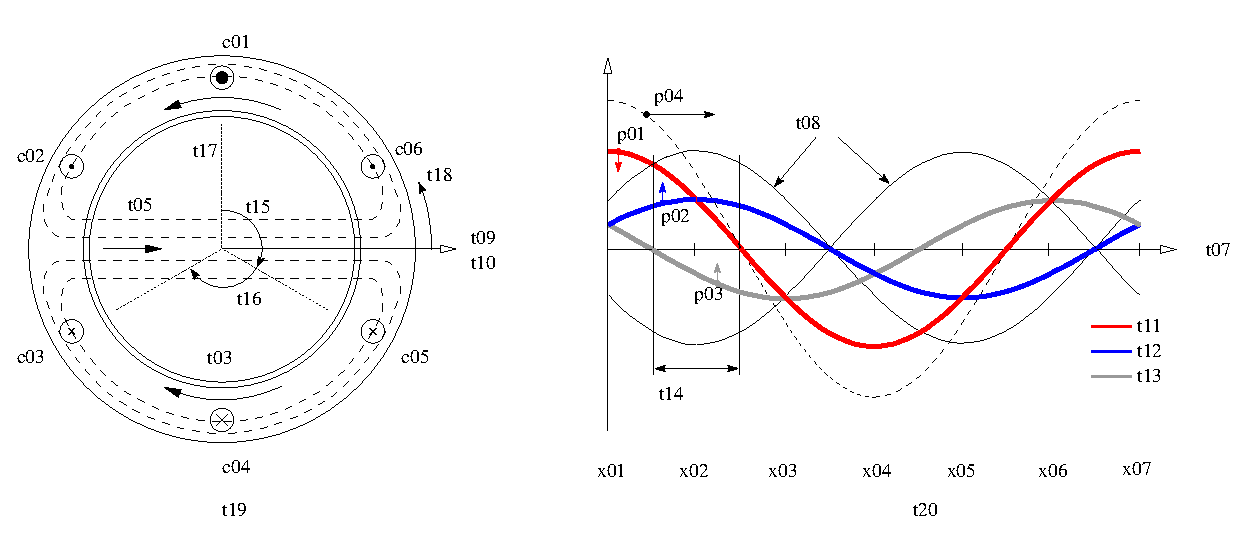
\includegraphics[width=1.00\textwidth]{figs/f_mmf_2.eps}
\end{psfrags}%
  \caption{The fundamental spatial mmf distribution for a three-phase machine}
	\label{fig:mmf_2}
\end{figure}

Fig.~\ref{fig:mmf_2}(b) shows graphically the mmf's of the three coils with $N_t$-turns. These are obtained by setting $m=3$ and applying the following three-phase currents 
\begin{equation}
  \label{eqn:3ph_i}
  \begin{aligned}
   i_1 &= \hat{I}\cos\left(\omega t \right) \\
   i_2 &= \hat{I}\cos\left(\omega t +\frac{2\pi}{3}\right) \\
   i_3 &= \hat{I}\cos\left(\omega t +\frac{4\pi}{3}\right) \\
  \end{aligned}
\end{equation}
to the functions in \eqref{eqn:F_theta_t_3}. The resultant mmf will rotate in a counterclockwise direction. At $t=0$ $i_2=i_3=-\frac{1}{2}i_1$, meaning the mmf of $F_2$ and $F_3$ will be half of $F_1$. As time starts to increase, any point on $F_1$ will move downward while points on $F_2$ and $F_3$ will start moving in an upward direction. The points are marked $p_1$ through $p_3$ in the figure. Contrary to this, any point on the resultant mmf will start moving in the right direction (counter-clockwise) as indicated by point $p_4$. As time increases the resultant mmf rotates as shown in Fig.~\ref{fig:rotating_wave}. The fundamental mmf is shown at time equal to zero and a time instant $t=t_1$.
\begin{figure}
	\centering
		\begin{psfrags}%
\psfragscanon

% text strings:
\psfrag{t01}{+1}
\psfrag{t02}{-1}
\psfrag{t03}{+3}
\psfrag{t04}{-3}
\psfrag{t05}{+2}
\psfrag{t06}{-2}
\psfrag{t07}[bc]{$t=0$}
\psfrag{t08}[bc]{$t=t_1$}

% Figure:
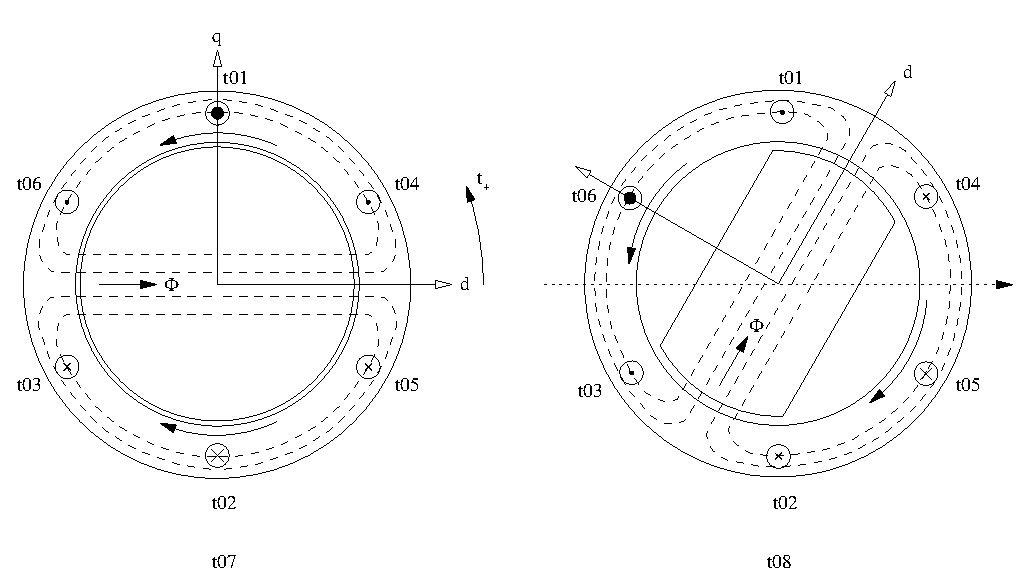
\includegraphics[width=1.00\textwidth]{figs/f_mmf_rotation.eps}
\end{psfrags}%
	\caption[Rotation of the resultant mmf]{Rotation of the resultant mmf by displacing~%
	the three positive coil sides along the stator periphery}
	\label{fig:rotating_wave}
\end{figure}

\subsection{Definition of the mmf envelope functions}\label{subsec:mmf_def}
As time continues, any point on the standing wave will have a minimum and maximum value between which it oscillates. If $p_2$ is used as an example, it will be bounded as shown in Fig.~\ref{fig:mmf_2}(b), thus forming an envelope. Similarly, the remaining phases will each form envelope functions. The bounding functions for all the phases are given by
\begin{equation}
  \label{eqn:f_bound}
  f_n(\theta) = \hat{F_n}\cos\left[\theta+\frac{2\pi}{m}(n-1) \right], 
  \quad 1 \leq n \leq m
\end{equation}
and the mmf of any of the phases will be bounded, i.e. 
\begin{equation}
  -\left|f_n(\theta)\right| \leq F_n(\theta ,t) \leq \left|f_n(\theta)\right|
\end{equation}

\subsection{Phase belt definition}\label{subsec:phasebelt_def}
The mmf envelope functions in section \ref{subsec:mmf_def} allow the definition of the phase belt in a unique way, which make it possible to allocate the stator slots that belong to a phase before the coil sides are assigned. 
\begin{defth}
In general, the interval $\left\langle \theta_1,\theta_2 \right\rangle$ for which any of the $m$ bounding functions in \eqref{eqn:f_bound} is greater than the remaining $(m-1)$ functions is defined as a phase belt, i.e. 
\begin{equation}
 \left|f_i(\theta)\right| > \left|f_n(\theta)\right|, \quad
 \begin{cases}
   1 \leq n \leq m \\
   n \neq i
 \end{cases}
\end{equation}
and the interval $\left\langle \theta_1,\theta_2 \right\rangle$ spans $\frac{2\pi}{2m}$ radians. 
\end{defth}
A useful parameter to define is the total number of phase belts around the air gap periphery, i.e. 
\begin{equation}
  \label{eqn:Np}
  N_p = \frac{2\pi p}{\left(\frac{2\pi}{2m}\right)}=p\cdot2m
\end{equation}
and means that the phase belt sequence (for three phases) given in \eqref{eqn:phasebelt_sequence} repeat itself $p$ times around the air gap periphery.

\subsection{Higher order harmonics}
A similar procedure as for the working harmonic can be used to derive the direction of rotation for the higher order harmonics. The decomposition of the air gap mmf means that the resultant mmf is the sum of an infinite number of rotating waves. The general expression for harmonic order (for three phases and six phase belts) of the air gap mmf harmonics is
\begin{equation}
  \label{eqn:harm_oder}
  \nu = 1+6g \quad g=0,\mp1,\mp2,\ldots
\end{equation}
and the speed of rotation is given by 
\begin{equation}
  \omega_{\nu} = \frac{\omega}{\nu}
\end{equation}
A positive value of $\nu$ means that the harmonic is rotating counter-clockwise and a negative $\nu$ means it rotates clockwise. This convention is valid for the coil arrangement as given in Fig.~\ref{fig:mmf_2}(a) and the currents in \eqref{eqn:3ph_i}. The rotation speed is proportional to the inverse of the harmonic order.

\section{Matrix representation of a winding}
In this section it will be shown that the winding layouts can be represented by means of two matrices. The first matrix will contain information on the ingoing coil sides of the coils while the second matrix will be that of the outgoing coil sides. The matrices are referred to as $\mathbf{M_1}$ and $\mathbf{M_{2}}$ for the ingoing and outgoing coil sides respectively. Both matrices have $n$ columns and $m$ rows. In addition, the number of columns equals the number of stator slots and the rows are equal to the number of phases, thus $m=m$\footnote{It is typical in mathematics that the number of rows is represented by $m$. Equally the number of phases of an electrical machine is also represented by $m$. Furthermore, $m_{11}$ is a matrix element while $m$ is the number of phases.} and $n=Q_s$. The matrices can be expressed as
\begin{equation}
  \label{eqn:M_matrix}
  \mathbf{M_1} = \left[
  \begin{array}{cccc}
     m_{11} & m_{12} & \ldots & m_{1n}\\
     m_{21} & m_{22} & \ldots & m_{2n}\\
     \vdots & \vdots & \ddots & \vdots\\
     m_{m1} & m_{m2} & \ldots & m_{mn}\\
  \end{array} \right]
  \quad
  \mathbf{M_2} = \left[
  \begin{array}{c c c c}
     m_{11} & m_{12} & \ldots & m_{1n}\\
     m_{21} & m_{22} & \ldots & m_{2n}\\
     \vdots & \vdots & \ddots & \vdots\\
     m_{m1} & m_{m2} & \ldots & m_{mn}\\
  \end{array} \right]  
\end{equation}
where
\begin{equation}
  \label{eqn:cij_set}
  m_{ij} \in \left\{-1,0,1\right\}
\end{equation}
and depends on the winding layout. In the rest of this section an algebraic method is derived to determine the matrix elements. The variables $n_1$ and $n_2$ are integers and will be used as loop variables later on in this chapter where the algorithm flowchart is explained. The subscripts $1$ and $2$ refer to the outer and inner loop respectively. 

\subsection{Slot vector}
For assigning the $Q_s$ slots to phase belts, the peripheral slot angle $\alpha$ needs to be defined in terms of the slot pitch $\tau_s$. If the slots have a regular distribution the angle between any two adjacent slots equals $\tau_s$. In the case of irregular distributed slots the average slot pitch will equal $\tau_s$. A regular and irregular distribution are shown in Fig.~\ref{fig:f_slotstar}. A vector is assigned to the centre of each stator slot. The exponential representation\footnote{Also known as Euler's formula.} of a vector is used, i.e.
\begin{equation} 
  e^{j\nu \alpha}=\cos(\nu \alpha)+j\sin(\nu \alpha)
\end{equation}
The variables $\nu$ and $\alpha$ are the harmonic order and slot peripheral angle respectively. All the vectors as shown in Fig.~\ref{fig:f_slotstar} are represented as a column matrix $\mathbf{v_{\nu}}$. The number of rows is equal to the number of slots, i.e.
\begin{equation}
  \label{eqn:slot_vector}
  \mathbf{v_{\nu}}=\left[
                         e^{j\nu\alpha_1} 
                         \: 
                         e^{j\nu\alpha_{n_2}} 
                         \:
                         \ldots 
                         \: e^{j\nu\alpha_{Q_s}}
                    \right]^{T}
   \qquad 1 \leq n_2 \leq Q_s                 
\end{equation}
where
\begin{equation}
  \label{eqn:slot_alpha}
  \alpha_{n_2} = \left\{ \begin{array}{lll}
	  \tau_s\left(n_2-1\right) && n_2 \;\text{odd}\\
	  \alpha_{n_2-1}+x\tau_s & 0<x<2 & n_2\;\text{even}
	\end{array} \right.
	\quad
	1 \leq n_2 \leq Q_s
\end{equation}
where the $\alpha$ accounts for both regular and irregular distributed stator slots. Setting $\nu=p$ means that the electrical slot angles\footnote{The electrical and mechanical slot have the following relationship: $\theta_e=p \theta_m$} for the working harmonic are obtained. 
\begin{figure}
	\centering
		\begin{psfrags}%
\psfragscanon

% text strings:
\psfrag{t01}{1}
\psfrag{t02}{$Q_s$}
\psfrag{t03}{$2\tau_s$}
\psfrag{t04}{$x\tau_s$}
\psfrag{t05}[bc]{(a) Regular distribution $x=1$}
\psfrag{t06}[bc]{(b) Irregular distribution $0<x<2$}

% Figure:
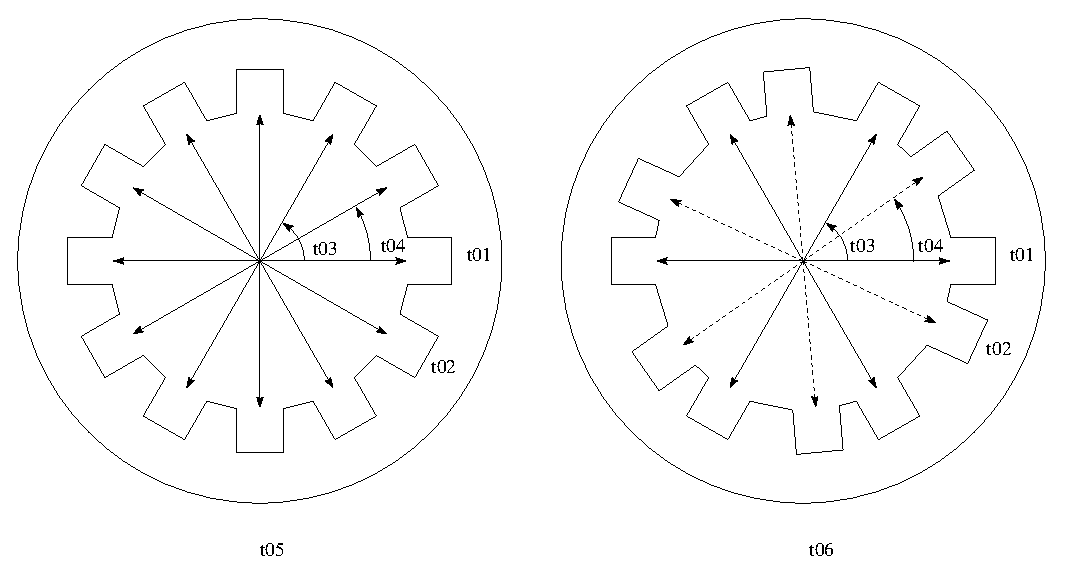
\includegraphics[width=1.00\textwidth]{figs/f_slotstar.eps}
\end{psfrags}%

	\caption{Star of slots}
	\label{fig:f_slotstar}
\end{figure}

\subsection{Phase belt constraint}
The phase belt constraint is used to determine the matrix elements $m_{ij}$ in \eqref{eqn:M_matrix}. From the slot angle $\alpha$ in \eqref{eqn:slot_vector} the corresponding electrical angle $\theta_e$ is obtained. A stator slot is assigned to the phase belt if the following constraint is true:
\begin{equation}	
 \label{eqn:phase_belt_constraint}
  \theta_1 \leq \theta_e  < \theta_2
  \quad
  \begin{cases}
    \left.
      \begin{array}{l}
        \theta_1 = \frac{2\pi}{2m}\left(n_1-1\right) \\
        \theta_2 = \frac{2\pi}{2m}n_1 \\
        1 \leq n_1 \leq N_p \\      
      \end{array}
    \right\} 
    \quad \mbox{phase belt boundaries} \\
    \left.
      \begin{array}{l}
        \theta_e = p\alpha_{n_2} \\
        1 \leq n_2 \leq Q_s \\      
      \end{array}    \right\} 
    \quad \mbox{electrical slot angle} \\
  \end{cases}
\end{equation} 
The phase belt constraint as given in \eqref{eqn:phase_belt_constraint} is characterised by the phase belt boundaries and the electrical slot angle, which are summerised as follows:
\begin{description}
	\item[Phase belt boundaries:] The total number of phase belts around the air gap~%
	periphery is given by \eqref{eqn:Np}. Each of the phase belts is bounded the by~%
	the angles $\theta_1$ and $\theta_2$.
	\item[Electrical slot angle:] The electrical slot angle is obtained by multiplying~%
	the peripheral slot angle in \eqref{eqn:slot_alpha} by the pole pair number. If~%
	the electrical angle for a given slot lies within the phase belt boundaries, it~%
	belongs to that phase belt.   
\end{description}
In order to assign the slot to a phase, it is necessary to know to which phase a given phase belt belongs. The phase can be determined in terms of the given phase belt number $n_1$ and the number of phases, i.e.
\begin{equation}
  \label{eqn:phase_belt_number}
  k = \mbox{mod}(n_1,2m)
  \quad
  \begin{cases}
    1 \leq n_1 \leq \ N_p \\
    2m \ \mbox{if} \ \mbox{mod}(n_1,2m)=0 \\
  \end{cases}
  \quad
  1\leq k \leq 2m
\end{equation}  
The value of $k$ as calculated in \eqref{eqn:phase_belt_number} corresponds to the phase belt number. Therefore, if the number of a given phase belt is known, the corresponding phase and its sign are calculated as follows:
\begin{equation}
  \label{eqn:phase_belt_number_2}
  \begin{aligned}
  \mbox{phase}&= 
    \left\{
    \begin{array}{ll}
	    k   & k \leq m\\
	    k-m & k > m
	  \end{array}
	  \right.
	  \\
	\mbox{sign}&=(-1)^{(k-1)} 
  \end{aligned}
\end{equation}	
If $m=3$ and $p=1$ the number of phase belts equals 6. Applying \eqref{eqn:phase_belt_number} and \eqref{eqn:phase_belt_number_2} will result in the phase belt sequence as given in \eqref{eqn:phasebelt_sequence}. 

\subsection{Algorithm flowchart}
The explanation of the algorithm is accompanied by the flowchart in Fig.~\ref{fig:flowchart} and greatly simplifies the understanding. For convenience the relevant equations or tables are included which makes it easier to follow the description. The algorithm only applies to symmetrical windings and the three major parts are summerised as follows:
\begin{description}
	\item[Outer loop:] The outer loop of the flowchart is used for the total number of phase belts as given in \eqref{eqn:Np}. The loop index $n_1$ (in the range $1\leq n_1 \leq N_p$) is used to calculate the given phase belt boundaries $\theta_1$ and $\theta_2$ as given in \eqref{eqn:phase_belt_constraint}. Since the $2m$ phase belts repeat themselves along the air gap periphery, the actual phase belt number $k$ in the phase belt sequence can be determined from $n_1$ as given in \eqref{eqn:phase_belt_number} and \eqref{eqn:phase_belt_number_2}.
	\item[Inner loop:] The inner loop has $n_2$ as index and is used to calculate the electrical angle for a given slot. If a slot is already assigned to a phase belt, the winding matrix will have an entry in the set $\{-1,1\}$. In this case the loop is skipped.   
	\item[Phase belt constraint:] This is the key step to allocate a stator slot. If the electrical angle lies within the phase belt boundaries, it belongs to the given phase belt. The row and column number for the ingoing matrix $\mathbf{M_1}$ are determined from the inner loop index $n_2$ and the given phase belt number. The row number for $\mathbf{M_2}$ is the same as for $\mathbf{M_1}$ and the column number is obtained from the coil pitch $y_d$.
\end{description}
The assignment of the stator slots as offered in this dissertation is unique and not presented in this way by any of the references consulted. 
\begin{figure}
	\centering
		\begin{psfrags}%
\psfragscanon

% text strings:
\psfrag{t01}[bc]{$n_1 = 1,N_p$}
\psfrag{t02}[bc]{$\theta_1, \; \theta_2$}
\psfrag{t04}[bc]{$k=f(n_1,m)$}
\psfrag{t05}[bc]{$n_2 = 1,Q_s$}
\psfrag{t07}[bc]{$\theta_1 \leq \theta_e < \theta_2$}
\psfrag{t08}[bc]{$i=f(k)$ and $h=-1^{(k-1)}$}
\psfrag{t09}[bc]{$\mathbf{M}_{1,ij}=h \quad j=n_2$}
\psfrag{t10}[bc]{$\mathbf{M}_{2,ij}=-h \quad j=f(n_2,y_d)$}
\psfrag{t11}[bc]{$n_2=Q_s$?}
\psfrag{t12}[bc]{$n_1=N_p$?}
\psfrag{t14}[bc]{Start}
\psfrag{t15}[bc]{$\mathbf{M}_{ij} \in \left\{-1,1\right\}$}

\psfrag{t16}[bc]{$\mbox{mod}(n_2,2)=0$}
\psfrag{t161}[bc]{\eqref{eqn:modn20}}
\psfrag{t18}[br]{Slots}
\psfrag{t19}[br]{Phase belts}

\psfrag{t20}[bc]{$\theta_e = f(\tau_s)$}
\psfrag{t21}[bl]{\eqref{eqn:phase_belt_number}}

\psfrag{t23}[bl]{\eqref{eqn:Np}}

\psfrag{t13}[bc]{End}
\psfrag{t29}[br]{Section \ref{sec:m_assignment}}
\psfrag{t30}[bl]{\eqref{eqn:phase_belt_constraint}}
\psfrag{t32}[bl]{\eqref{eqn:matrix_element}}
\psfrag{t33}[bc]{y}
\psfrag{t34}[bc]{n}

% Figure:
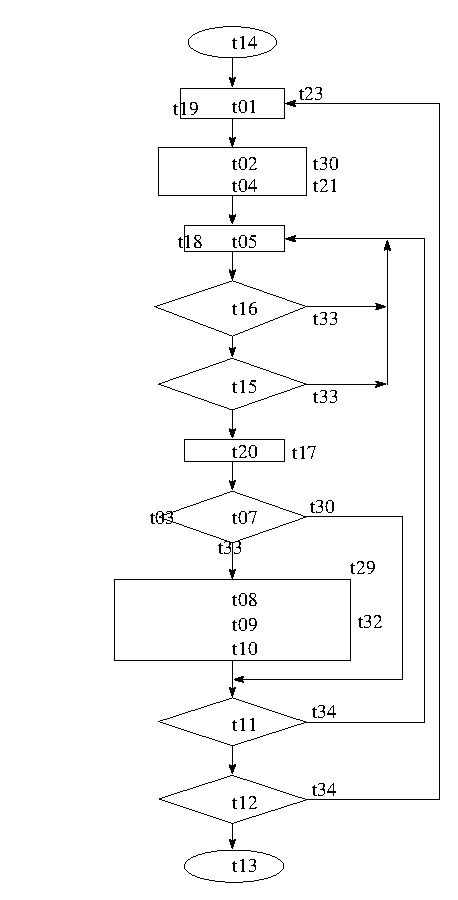
\includegraphics[width=0.55\textwidth]{figs/f_flowchart.eps}
\end{psfrags}%
	\caption{Flowchart to allocate the stator slots}
	\label{fig:flowchart}
\end{figure}

\subsection{Matrix element assignment}\label{sec:m_assignment}
Once the phase belt constraint is fulfilled, the slot is allocated and the next step is to assign one of the values in the set given in \eqref{eqn:cij_set}. Actually only the sign needs to be determined. Since the phase belt sequence is alternating, the sign can be obtained from the phase belt itself. Following the flowchart through to the point where the test is performed, it is noticed that the matrix column number for $\mathbf{M}_1$ is given by the loop index variable $n_2$. The entry has the value  $(-1)^{(k-1)}$, where $k$ is given in \eqref{eqn:phase_belt_number}. The determination of the row, column and matrix element are summerised as follows\footnote{The method was only tested for $m=3,5,7,\ldots$}: 
\begin{equation}
  \label{eqn:matrix_element}
  \begin{aligned}
  i &= 
  \left\{ 
    \begin{array}{ll}
	    k   & k \leq m\\
	    k-m & k > m
	  \end{array}
	  \qquad 
	\right\}
	\mbox{row number}
	\\
	h &= (-1)^{(k-1)} 
	\quad 
	\mbox{matrix element sign} 
	\\
	j &= 
  \left\{ 
    \begin{array}{ll}
	    n_2+y_d   & n_2+y_d \leq Q_s \\
	    \mbox{mod}\bigl((n_2+y_d),Q_s\bigr) & n_2+y_d > Q_s
	  \end{array} 
	  \quad
	\right\}
	\mbox{column number}
	\end{aligned}
\end{equation}

\section{Properties of the winding matrix}
Presenting the winding in matrix form is very compact and has advantages in machine analysis. The matrix contains all the information of the winding arrangement in the stator slots. This allows the construction of the voltage phasor which is necessary to calculate the winding factor. In addition, the slot mmf can be obtained from the column data. The properties of the matrix are summerised as follows:
\begin{itemize*}
	\item if the winding is symmetrical, the number of assigned elements in all~%
	the rows are equal;
	\item the number of columns is equal to the number of stator slots;
	\item the number of rows is equal to the number of phases;
	\item for a single layer winding there is only one nonzero element in a column;
	\item a double layer winding has two nonzero elements in a row; and
	\item the matrix is valid for both a fixed and variable slot pitch.
\end{itemize*}
In the rest of this section the winding matrix is used to calculate the winding factor and the slot mmf.

\subsection{Winding factor}
With $\mathbf{M}_1$ and $\mathbf{M}_2$ assigned, the winding factor for any harmonic can be calculated as the product between the matrices and the slot vector as given in \eqref{eqn:slot_vector}. This means that a row of the winding matrix is multiplied by the slot vector column matrix. The matrix product means that all the vectors belonging to the same phase are added and for the case $\nu=p$ equals
\begin{equation}
  \label{eqn:m1_m2_exp}
  (m_{1,i1}+m_{2,i1})e^{jp\alpha_1}+(m_{1,i2}+m_{2,i2})e^{jp\alpha_2}+\ldots+
  (m_{1,iQ_s}+m_{2,iQ_s})e^{jp \alpha_{Q_s}}
\end{equation}
If the slot vector does not belong to the current phase, the coefficient
\begin{equation} 
  \left(m_{1,ij}+m_{2,ij}\right)
\end{equation} 
is zero. Furthermore, the product should be normalised. Since the total number of vectors is related to the coils per phase it should be multiplied by $\left(2\frac{Q_c}{3}\right)^{-1}$, i.e.
\begin{equation}
  \label{eqn:winding_factor}
  \xi_{\nu} = \frac{3}{2Q_c}
  \Bigl[
    \mathbf{M}_1\mathbf{v_{\nu}}+\mathbf{M}_2\mathbf{v_{\nu}}
  \Bigr], 
  \quad \in \mathbb{C}
\end{equation}
The result \eqref{eqn:winding_factor} present the winding factor as a complex number and the absolute value is to be used as a reduction factor for the sinusoidally induced voltage in \eqref{eqn:ui}. Writing $\xi_{\nu}$ as
\begin{equation}
  \xi_{\nu} = a_{\nu}+jb_{\nu}
\end{equation}
the phase angle is calculated as 
\begin{equation}
  \theta_{\nu} = \arctan\left(\frac{b_{\nu}}{a_{\nu}}\right)
\end{equation}
The phase angle (in electrical radians) gives information on the position of the winding axes\footnote{The winding axes in the present dissertation refer to the current anti-node axis and the magnetic axis. This is shown in Fig.~\ref{fig:determ_axis}.} relative to the first slot. The two winding axes associated with each phase are called
\begin{itemize*}
	\item the current sheet anti-node axis and
	\item the magnetic axis
\end{itemize*}
of the winding. A positive phase angle means that both winding axes have moved clockwise with respect to the first slot. The winding axes are a very import quantities in machine design. When the machine is supplied with a source, a rotating magnetic flux wave is generated. This reacts with the flux generated by the flux of the permanent magnets on the rotor. In order to control the resultant flux, it is necessary to know the exact position of the winding axes.  

\subsection{Current sheet anti-node axis}\label{subsec:current_sheet}
Equation \eqref{eqn:F_theta_t_1} describes the space fundamental component of the mmf produced by the current in phase 1. It can be seen as the mmf wave produced by a finely divided sinusoidally distributed current sheet placed on the inner periphery of the stator. The position of the anti-node with maximum deviation is given by $\theta_{an}$. The relative position of $\theta_{an}$ with respect to the first slot is given by
\begin{equation}
  \label{eqn:theta_an}
  \theta_{an_{\nu}} = -
  \frac{\theta_{\nu}}{p}
\end{equation} 

\subsection{Magnetic axis}\label{subsec:magnetic_axis}
The axis along which the flux is directed when current is flowing in the coil, is defined as the magnetic axis. This is the same position where the current sheet has a node. The relative position of the magnetic axis $\theta_m$ with respect to the first slot is given by
\begin{equation}
  \label{eqn:theta_m}
  \theta_{m_{\nu}} = -
  \frac{\left(\theta_{\nu}+\frac{\pi}{2}\right)}{p}
\end{equation} 
The winding magnetic axis lags the current sheet anti-node axis by $\frac{\pi}{2}$
radians.

\subsection{Slot mmf}\label{subsec:slot_mmf}
The amp\`ere-turns in each slot can be obtained from the matrix winding columns. Both the matrices $\mathbf{M_1}$ and $\mathbf{M_2}$ contain the coil side information for the ingoing and outgoing coil sides respectively. The total amp\`ere-turns of a coil side is the product of its value in the winding matrix with the number of coil turns $N_t$. The direction of the current is given by the sign of the element. Therefore to get the total amp\`ere-turns in the slot, the amp\`ere-turns of the coil sides must be added. For a three-phase winding the slot mmf $F_{slot}$ of the $k^{th}$ slot is calculated as  
\begin{equation}
  \label{eqn:slot_mmf}
  \begin{aligned}
  F_{slot,k} &= N_t i_1(m_{1,1k}+m_{2,1k})+
                N_t i_2(m_{1,2k}+m_{2,2k})+
                N_t i_3(m_{1,3k}+m_{2,3k}) \\
             &= N_t\sum_{n=1}^{3}i_n \left(m_{1,nk}+m_{2,nk}\right) 
  \end{aligned}
\end{equation}

\section{Examples}
The derived theory presented in this chapter is now illustrated by means of examples. The examples are summerised as follows:
\begin{description}
	\item[Winding factor tables:] The winding factors for different slot and pole pair combinations are calculated for single and double layer non-overlapping windings. The results presented are used to derive an expression to find the feasible range for the number of pole pairs, given the number of stator slots. 
	\item[Slot mmf and current sheet:] The prototype stator with 30 slots is used as an example. By choosing different pole pair numbers, it is shown how to obtain both a single and double layer winding. In each case a non-overlapping and overlapping winding are explained.
\end{description}
  
\subsection{Winding factor table}\label{subsec:wind_fac_table}
The results are given in Tab.~\ref{tab:xi_single} Tab.~\ref{tab:xi_double} for single and double layer non-overlapping windings respectively. Only those slot and pole combinations for which the winding factor is greater than or equal to $\frac{\sqrt{3}}{2}$ are given. Those combinations that do not fulfill the condition in \eqref{eqn:feasibility} are marked as not applicable. Presenting the winding factors in a table is helpful to identify the relationship between the number of stator slots and the number of poles which results in the best combinations. Only the winding factors for the working harmonic are presented. 

The winding factors for single windings are calculated for pole pairs in the range from 4 to 28, whereas the number of stator slots range from 12 to 84. Although the focus in the present dissertation is on single layer non-overlapping windings, the winding factors for double layer windings are given as well. The winding factors are calculated for pole pairs in the range from 4 to 16, whereas the number of stator slots ranges from 12 to 48.
\begin{table}[htbp]
	\caption{$\xi_p \times \num{e-3}$ for single layer non-overlapping windings}
	\label{tab:xi_single}
	\centering
	 \begin{tabular}
		{|l||c|c|c|c|c|c|c|c|c|c|c|c|c|}\cline{2-14}
		\multicolumn{1}{c}{}& \multicolumn{13}{|c|}{$Q_s$}
		\\\hline
		$p$&12 &18 &24 &30 &36 &42 &48 &54 &60 &66 &72 &78 &84  \\\hline
		4  &866&   &   &   &   &   &   &   &   &   &   &   &    \\
		5  &966&   &   &   &   &   &   &   &   &   &   &   &    \\
		6  &na &866&   &   &   &   &   &   &   &   &   &   &    \\
		7  &966&902&   &   &   &   &   &   &   &   &   &   &    \\
		8  &866&945&866&   &   &   &   &   &   &   &   &   &    \\
		9  &   &na &na &   &   &   &   &   &   &   &   &   &    \\
		10 &   &945&966&866&   &   &   &   &   &   &   &   &    \\
		11 &   &902&958&874&   &   &   &   &   &   &   &   &    \\
		12 &   &866&na &na &866&   &   &   &   &   &   &   &    \\
		13 &   &   &958&940&870&   &   &   &   &   &   &   &    \\
		14 &   &   &966&950&na &866&   &   &   &   &   &   &    \\
		15 &   &   &na &na &966&na &   &   &   &   &   &   &    \\
		16 &   &   &866&950&na &na &866&   &   &   &   &   &    \\
		17 &   &   &   &940&956&na &859&   &   &   &   &   &    \\
		18 &   &   &   &na &na &na &na &866&   &   &   &   &    \\
		19 &   &   &   &866&956&na &907&na &   &   &   &   &    \\
		20 &   &   &   &866&na &na &966&na &866&   &   &   &    \\
		21 &   &   &   &   &966&na &na &na &na &   &   &   &    \\
		22 &   &   &   &   &na &na &958&na &954&866&   &   &    \\
		23 &   &   &   &   &870&na &956&na &893&na &   &   &    \\
		24 &   &   &   &   &866&na &na &na &na &na &866&   &    \\
		25 &   &   &   &   &   &na &956&na &966&na &848&   &    \\
		26 &   &   &   &   &   &na &958&na &na &na &870&866&    \\	
		27 &   &   &   &   &   &na &na &na &na &na &na &na &    \\	
		28 &   &   &   &   &   &866&966&na &na &na &na &na &866 \\\hline			
	\end{tabular}
\end{table}
 
\begin{table}[htbp]
	\caption{$\xi_p \times \num{e-3}$ for double layer non-overlapping windings }
	\label{tab:xi_double}
	\centering
  \begin{tabular}
		{|l||c|c|c|c|c|c|c|c|c|c|c|c|c|}\cline{2-14}
		\multicolumn{1}{c}{}& \multicolumn{13}{|c|}{$Q_s$}
		\\\hline
		$p$&12 &15 &18 &21 &24 &27 &30 &33 &36 &39 &42 &45 &48  \\\hline
		4  &866&   &   &   &   &   &   &   &   &   &   &   &    \\
		5  &930&866&   &   &   &   &   &   &   &   &   &   &    \\
		6  &na &na &866&   &   &   &   &   &   &   &   &   &    \\
		7  &930&950&900&866&   &   &   &   &   &   &   &   &    \\
		8  &866&950&950&890&866&   &   &   &   &   &   &   &    \\
		9  &   &na &na &na &na &866&   &   &   &   &   &   &    \\
		10 &   &866&950&950&930&880&866&   &   &   &   &   &    \\
		11 &   &   &900&950&950&920&870&866&   &   &   &   &    \\
		12 &   &   &866&na &na &950&na &na &866&   &   &   &    \\
		13 &   &   &   &890&950&950&940&900&870&866&   &   &    \\
		14 &   &   &   &866&930&950&950&930&900&860&866&   &    \\
		15 &   &   &   &   &na &950&na &na &930&na &na &866&    \\
		16 &   &   &   &   &866&920&950&950&950&920&890&860&866 \\\hline			
		\end{tabular}
\end{table}

From the results in Tab.~\ref{tab:xi_single} and Tab.~\ref{tab:xi_double} the number of slots per pole and phase which results in a winding with suitable winding factors is given by
\begin{equation}
  \frac{1}{4} \leq q \leq \frac{1}{2}
\end{equation}
The result is the same as presented by \cite{cros_2002} and \cite{skaar_2006}. Using this result, the range of pole pairs for a given number of slots can be expressed as follows:
\begin{equation}
  \frac{Q_s}{m} \leq p \leq \frac{2Q_s}{m}
  \quad
  \left\{
  \begin{array}{ll}
  Q_s \in \left\{6,12,18,\ldots\right\} & \mbox{single layer}\\
  \:  & \: \\
  Q_s \in \left\{3,6,9,\ldots\right\} & \mbox{double layer}\\
  \end{array}
  \right.
\end{equation} 

\subsection{Slot mmf and current sheet}
This section entails examples of overlapping and non-overlapping windings with 30 stator slots. The classification parameters $q$, $q_c$ and $y_d$ (as given in Tab.~\ref{tab:Example_table}) are used to classify the windings according to the scheme in Fig.~\ref{fig:classification}. Additionally, for the selected number of pole pairs the winding factor, slot mmf and current sheet are calculated. It is important to mention that the choice of the position of the reference slot will determine the rotation direction of the resulting rotating field. It is desirable to have a field rotating in a counter-clockwise direction, since this is the positive direction in a polar coordinate system. To achieve this, the stator is rolled flat with the top part of the slots facing upwards. 
\begin{table}[htbp]
	\caption{Different pole pair combinations with $Q_s = 30$}
	\label{tab:Example_table}
	\centering	
	 \begin{tabular}{ccccccccccccccccc}
	  \toprule
		$Q_s$ &$p$ &$Q_c$ &$n_l$& $y_p$ &$y_d$ &$q$ &$q_c$ & $Q_b$ & $t$ &
		$\xi_p$ &$\xi_{5p}$ &$\xi_{7p}$ &Figure
		\\
		\midrule
		30    &10  &15  &1   &$\frac{3}{2}$   &1   &$\frac{1}{2}$ &  $\frac{1}{4}$& 6 & 5 &
		0.866   &0.866      &0.866      &%
		\ref{fig:Main_non-overlapping_single}\subref{fig:f_Qs30_p10_1}
		\\
		30    &10  &30  &2    &$\frac{3}{2}$  &1   &$\frac{1}{2}$ &  $\frac{1}{2}$ & 3&10 &
		0.866   &0.866      &0.866      &%
		\ref{fig:Main_non-overlapping_double}\subref{fig:f_Qs30_p10_2}
		\\    
		30    &5   &15  &1    &3 &3  &1 &  $\frac{1}{2}$ & 6 & 5  &
		1.0     &1.0        &1.0        &%
		\ref{fig:Main_single_overlapping}\subref{fig:f_Qs30_5_1}
		\\
		30    &5   &30  &2    &3 &3  &1 &  1 & 6 & 5  &
		1.0     &1.0        &1.0        &%
		\ref{Main_double_overlapping}\subref{fig:f_Qs30_p5_2}   
		\\
		\bottomrule			
	 \end{tabular}
\end{table} 

\subsubsection{Single layer non-overlapping}
Fig.~\ref{fig:Main_non-overlapping_single}\subref{fig:single_layer} shows an illustration of a single layer non-overlapping winding. There is only one coil side in each stator slot and the slot pitch could be either regular or irregular. An irregular slot pitch means that the coil pitch can be varied to improve the winding factor. Depending on the design criteria, it can also be used to improve the torque ripple. Since the outgoing coils are given by the coil pitch $y_d$, only every second slot needs to be assigned to a phase belt.  

The example chosen is that of the prototype machine with 30 slots and 10 pole pairs. 
From Tab.~\ref{tab:Example_table} the values for $q$ and $q_c$ are $\frac{1}{2}$ and $\frac{1}{4}$ respectively. The basic winding is determined using $q_c$ and has one  coil per phase distributed over 4 poles. In total the basic winding has 6 slots. The winding has a sub-harmonic with 5 pole pairs. Since it is a single layer winding the number of coils is half the number of stator slots. The coil pitch equals one and this is a fractional slot winding. For convenience only the basic winding matrix elements for $\mathbf{M_1}$ and $\mathbf{M_2}$ are given as
\begin{equation}
  \mathbf{M_{1,b}} = 
  \begin{pmatrix}
  1&0&0&0&0&0\\
  0&0&1&0&0&0\\
  0&0&0&0&1&0\\
  \end{pmatrix} \
  \mathbf{M_{2,b}} = 
  \begin{pmatrix}
  0&-1&0&0 &0&0 \\
  0&0 &0&-1&0&0 \\
  0&0 &0&0 &0&-1\\
  \end{pmatrix} 
\end{equation}
To obtain the complete winding matrix, the matrix of the basic winding is repeated five times. For the ingoing coil side matrix this means
\begin{equation}
  \mathbf{M_1} = 
  \begin{bmatrix}
  \mathbf{M_{1,b}}&\mathbf{M_{1,b}}&\mathbf{M_{1,b}}&
  \mathbf{M_{1,b}}&\mathbf{M_{1,b}}
  \end{bmatrix}  
\end{equation}
The winding matrix is used to obtain the slot mmf $F_{slot}$ from \eqref{eqn:slot_mmf} as shown in the lower part of~%
Fig.~\ref{fig:Main_non-overlapping_single}\subref{fig:f_Qs30_p10_1}. The dashed line in the mmf plot is the current sheet. In the top part of the figure the winding factors are shown as well. From the figure it is clear that the winding factors are periodic with the number of stator slots. In the example the peripheral slot angle was calculated setting $x=1$ in \eqref{eqn:slot_alpha}. Therefore, this is a regular distribution of the stator slots.
\begin{figure}[htbp]
	\centering
	\begin{psfrags}%
\psfragscanon

% text strings:
\psfrag{t01}{{\tiny Constant pitch, $2\tau_s$}}
\psfrag{t02}{{\tiny Variable slot pitch, $x \tau_s$}}
\psfrag{t03}{{\tiny Direction of coil assignment}}
\psfrag{t04}{{\tiny 1}}
\psfrag{t05}{{\tiny 2}}
\psfrag{t06}{{\tiny 3}}
\psfrag{t07}{{\tiny 4}}

% Figure:

\subfloat[Winding layout\label{fig:single_layer}]{%	
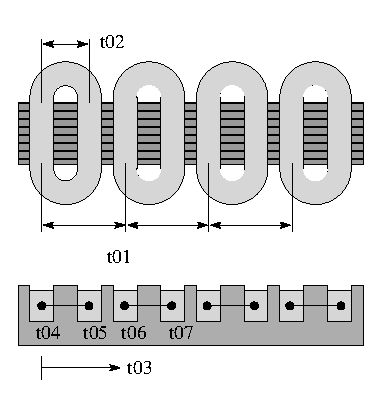
\includegraphics[height=7cm]{figs/f_single_layer.eps}}

\end{psfrags}%
	\vspace{1cm}
	% This file is generated by the MATLAB m-file laprint.m. It can be included
% into LaTeX documents using the packages graphicx, color and psfrag.
% It is accompanied by a postscript file. A sample LaTeX file is:
%    \documentclass{article}\usepackage{graphicx,color,psfrag}
%    \begin{document}% This file is generated by the MATLAB m-file laprint.m. It can be included
% into LaTeX documents using the packages graphicx, color and psfrag.
% It is accompanied by a postscript file. A sample LaTeX file is:
%    \documentclass{article}\usepackage{graphicx,color,psfrag}
%    \begin{document}\input{f_Qs_30_p_10_1}\end{document}
% See http://www.mathworks.de/matlabcentral/fileexchange/loadFile.do?objectId=4638
% for recent versions of laprint.m.
%
% created by:           LaPrint version 3.16 (13.9.2004)
% created on:           12-Nov-2008 21:44:16
% eps bounding box:     17.5 cm x 13.125 cm
% comment:              
%
\begin{psfrags}%
\psfragscanon%
%
% text strings:
\psfrag{s05}[b][b]{{\tiny $\xi_{10}$}}%
\psfrag{s06}[b][b]{{\tiny $\xi_{50}$}}%
\psfrag{s07}[b][b]{{\tiny $\xi_{70}$}}%
\psfrag{s08}[t][t]{{\tiny $\nu$}}%
\psfrag{s09}[b][b]{{\tiny $\xi_{\nu}$}}%
\psfrag{s10}[t][t]{{\tiny Slot number}}%
\psfrag{s11}[b][b]{{\tiny $F_{slot}/\SI{}{A}$}}%
%
% xticklabels:
\psfrag{x01}[t][t]{{\tiny 0}}%
\psfrag{x02}[t][t]{{\tiny 5}}%
\psfrag{x03}[t][t]{{\tiny 10}}%
\psfrag{x04}[t][t]{{\tiny 15}}%
\psfrag{x05}[t][t]{{\tiny 20}}%
\psfrag{x06}[t][t]{{\tiny 25}}%
\psfrag{x07}[t][t]{{\tiny 30}}%
\psfrag{x08}[t][t]{{\tiny 0}}%
\psfrag{x09}[t][t]{{\tiny 10}}%
\psfrag{x10}[t][t]{{\tiny 20}}%
\psfrag{x11}[t][t]{{\tiny 30}}%
\psfrag{x12}[t][t]{{\tiny 40}}%
\psfrag{x13}[t][t]{{\tiny 50}}%
\psfrag{x14}[t][t]{{\tiny 60}}%
\psfrag{x15}[t][t]{{\tiny 70}}%
\psfrag{x16}[t][t]{{\tiny 80}}%
\psfrag{x17}[t][t]{{\tiny 90}}%
%
% yticklabels:
\psfrag{v01}[r][r]{{\tiny -1}}%
\psfrag{v02}[r][r]{{\tiny -0.5}}%
\psfrag{v03}[r][r]{{\tiny 0}}%
\psfrag{v04}[r][r]{{\tiny 0.5}}%
\psfrag{v05}[r][r]{{\tiny 1}}%
\psfrag{v06}[r][r]{{\tiny 0}}%
\psfrag{v07}[r][r]{{\tiny 0.1}}%
\psfrag{v08}[r][r]{{\tiny 0.2}}%
\psfrag{v09}[r][r]{{\tiny 0.3}}%
\psfrag{v10}[r][r]{{\tiny 0.4}}%
\psfrag{v11}[r][r]{{\tiny 0.5}}%
\psfrag{v12}[r][r]{{\tiny 0.6}}%
\psfrag{v13}[r][r]{{\tiny 0.7}}%
\psfrag{v14}[r][r]{{\tiny 0.8}}%
\psfrag{v15}[r][r]{{\tiny 0.9}}%
\psfrag{v16}[r][r]{{\tiny 1}}%
\psfrag{v17}[r][r]{{\tiny 1.1}}%
%
% Figure:

\subfloat[Slot mmf and winding factors\label{fig:f_Qs30_p10_1}]{%
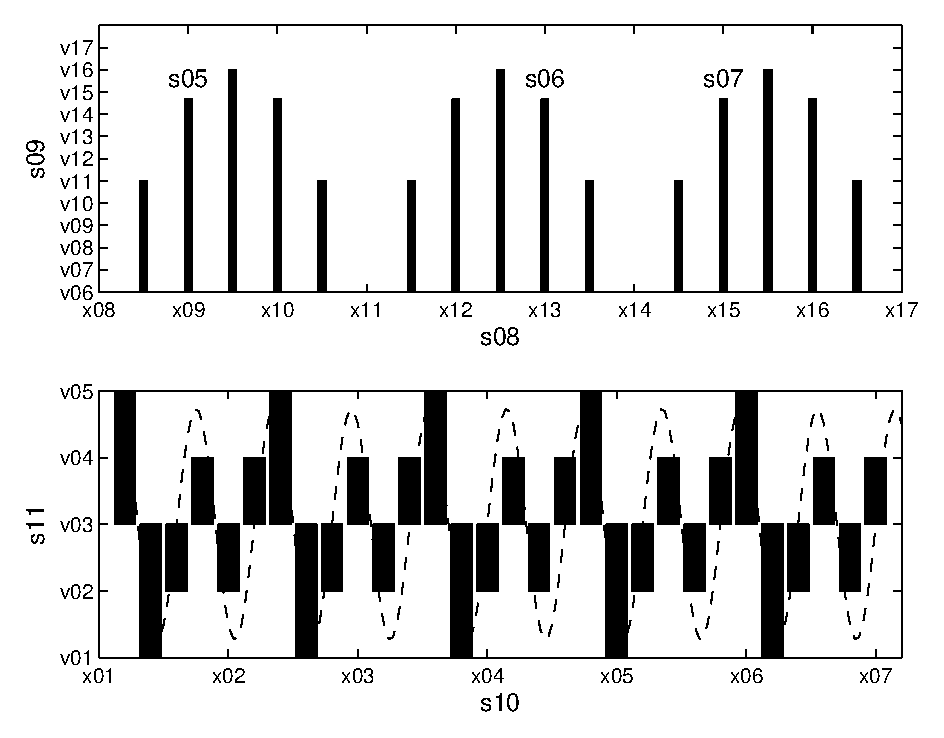
\includegraphics[width=0.9\textwidth]{figs/f_Qs_30_p_10_1.eps}}%
\end{psfrags}%
%
% End f_Qs_30_p_10_1.tex
\end{document}
% See http://www.mathworks.de/matlabcentral/fileexchange/loadFile.do?objectId=4638
% for recent versions of laprint.m.
%
% created by:           LaPrint version 3.16 (13.9.2004)
% created on:           12-Nov-2008 21:44:16
% eps bounding box:     17.5 cm x 13.125 cm
% comment:              
%
\begin{psfrags}%
\psfragscanon%
%
% text strings:
\psfrag{s05}[b][b]{{\tiny $\xi_{10}$}}%
\psfrag{s06}[b][b]{{\tiny $\xi_{50}$}}%
\psfrag{s07}[b][b]{{\tiny $\xi_{70}$}}%
\psfrag{s08}[t][t]{{\tiny $\nu$}}%
\psfrag{s09}[b][b]{{\tiny $\xi_{\nu}$}}%
\psfrag{s10}[t][t]{{\tiny Slot number}}%
\psfrag{s11}[b][b]{{\tiny $F_{slot}/\SI{}{A}$}}%
%
% xticklabels:
\psfrag{x01}[t][t]{{\tiny 0}}%
\psfrag{x02}[t][t]{{\tiny 5}}%
\psfrag{x03}[t][t]{{\tiny 10}}%
\psfrag{x04}[t][t]{{\tiny 15}}%
\psfrag{x05}[t][t]{{\tiny 20}}%
\psfrag{x06}[t][t]{{\tiny 25}}%
\psfrag{x07}[t][t]{{\tiny 30}}%
\psfrag{x08}[t][t]{{\tiny 0}}%
\psfrag{x09}[t][t]{{\tiny 10}}%
\psfrag{x10}[t][t]{{\tiny 20}}%
\psfrag{x11}[t][t]{{\tiny 30}}%
\psfrag{x12}[t][t]{{\tiny 40}}%
\psfrag{x13}[t][t]{{\tiny 50}}%
\psfrag{x14}[t][t]{{\tiny 60}}%
\psfrag{x15}[t][t]{{\tiny 70}}%
\psfrag{x16}[t][t]{{\tiny 80}}%
\psfrag{x17}[t][t]{{\tiny 90}}%
%
% yticklabels:
\psfrag{v01}[r][r]{{\tiny -1}}%
\psfrag{v02}[r][r]{{\tiny -0.5}}%
\psfrag{v03}[r][r]{{\tiny 0}}%
\psfrag{v04}[r][r]{{\tiny 0.5}}%
\psfrag{v05}[r][r]{{\tiny 1}}%
\psfrag{v06}[r][r]{{\tiny 0}}%
\psfrag{v07}[r][r]{{\tiny 0.1}}%
\psfrag{v08}[r][r]{{\tiny 0.2}}%
\psfrag{v09}[r][r]{{\tiny 0.3}}%
\psfrag{v10}[r][r]{{\tiny 0.4}}%
\psfrag{v11}[r][r]{{\tiny 0.5}}%
\psfrag{v12}[r][r]{{\tiny 0.6}}%
\psfrag{v13}[r][r]{{\tiny 0.7}}%
\psfrag{v14}[r][r]{{\tiny 0.8}}%
\psfrag{v15}[r][r]{{\tiny 0.9}}%
\psfrag{v16}[r][r]{{\tiny 1}}%
\psfrag{v17}[r][r]{{\tiny 1.1}}%
%
% Figure:

\subfloat[Slot mmf and winding factors\label{fig:f_Qs30_p10_1}]{%
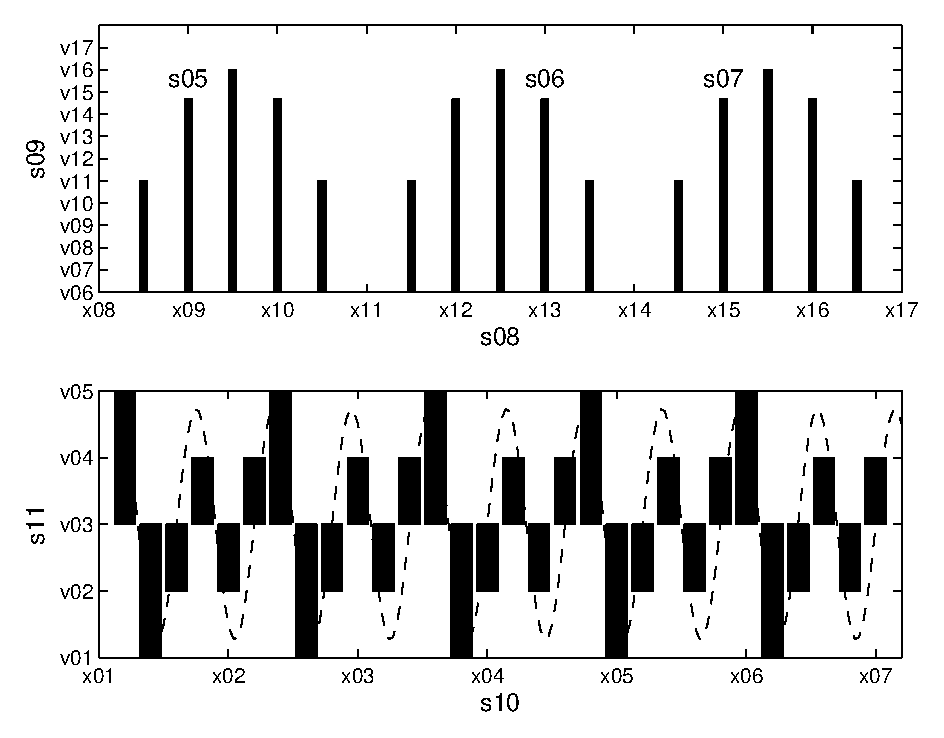
\includegraphics[width=0.9\textwidth]{figs/f_Qs_30_p_10_1.eps}}%
\end{psfrags}%
%
% End f_Qs_30_p_10_1.tex

	\caption{Non-overlapping single layer winding}
	\label{fig:Main_non-overlapping_single}
\end{figure}

\subsubsection{Double layer non-overlapping}
Fig.~\ref{fig:Main_non-overlapping_double}\subref{fig:dlw_yd_eq_1} shows a non-overlapping double layer winding. Each stator slot has two coil sides. Moreover, each slot needs to be assigned to a phase belt. 

The prototype stator with 30 slots is used with 10 pole pairs. This is a double layer winding and the number of slots is equal to the number of coils. Both $q$ and $q_c$ and the basic winding has 3 slots. The lowest harmonic has 10 pole pairs which is the same as the working harmonic. Therefore, the winding has no sub-harmonics. The matrix elements of the basic winding are 
\begin{equation}
  \mathbf{M_{1,b}} = 
  \begin{pmatrix}
  1&0&0\\
  0&0&1\\
  0&1&0\\ 
  \end{pmatrix} \
  \mathbf{M_{2,b}} = 
  \begin{pmatrix}
  0 &-1&0\\
  -1&0&0\\
  0&0&-1\\ 
  \end{pmatrix} 
\end{equation}
The winding factors and slot mmf are directly obtained from the winding matrix as shown in Fig.~\ref{fig:Main_non-overlapping_double}\subref{fig:f_Qs30_p10_2}. The current sheet that corresponds to the working harmonic is included.
\begin{figure}[htbp]
	\centering
	\begin{psfrags}%
\psfragscanon

% text strings:
\psfrag{t01}[bc]{{\tiny $y_d$}}
\psfrag{t02}[bl]{{\tiny Direction of coil assignment}}
\psfrag{t03}{{\tiny 1}}
\psfrag{t04}{{\tiny 2}}
\psfrag{t05}{{\tiny 3}}
\psfrag{t06}{{\tiny 4}}
\psfrag{t07}{{\tiny 5}}

% Figure:

\subfloat[Winding layout\label{fig:dlw_yd_eq_1}]{%
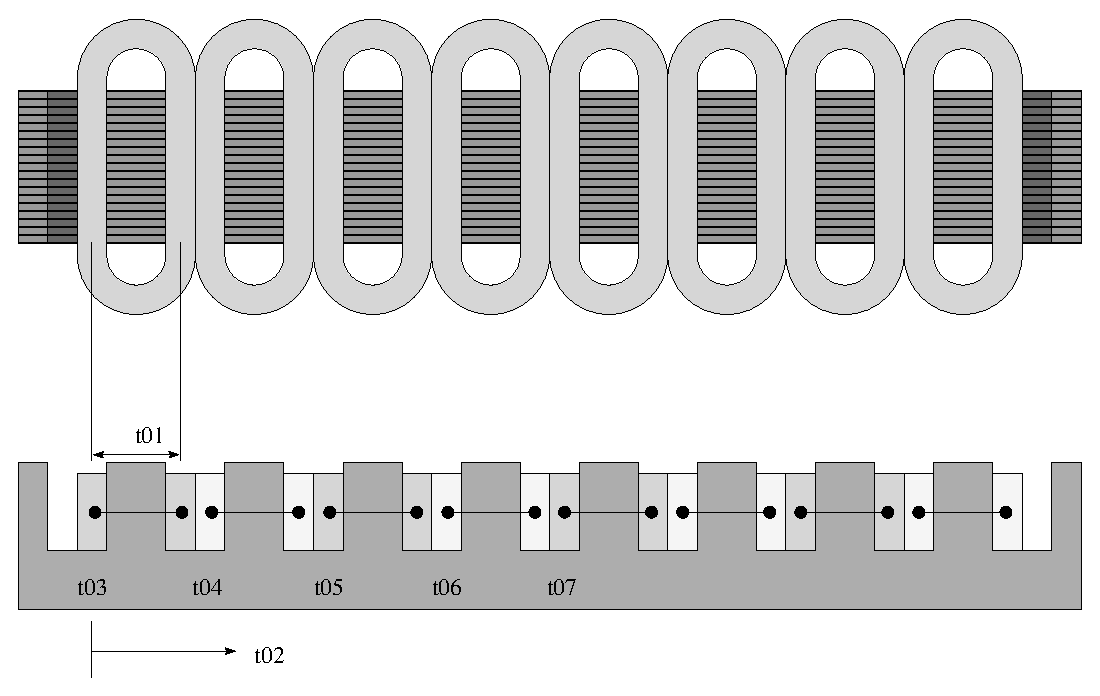
\includegraphics[height=7cm]{figs/f_double_layer_type2.eps}}
\end{psfrags}%

	\vspace{1cm}
  % This file is generated by the MATLAB m-file laprint.m. It can be included
% into LaTeX documents using the packages graphicx, color and psfrag.
% It is accompanied by a postscript file. A sample LaTeX file is:
%    \documentclass{article}\usepackage{graphicx,color,psfrag}
%    \begin{document}% This file is generated by the MATLAB m-file laprint.m. It can be included
% into LaTeX documents using the packages graphicx, color and psfrag.
% It is accompanied by a postscript file. A sample LaTeX file is:
%    \documentclass{article}\usepackage{graphicx,color,psfrag}
%    \begin{document}\input{f_Qs_30_p_10_2}\end{document}
% See http://www.mathworks.de/matlabcentral/fileexchange/loadFile.do?objectId=4638
% for recent versions of laprint.m.
%
% created by:           LaPrint version 3.16 (13.9.2004)
% created on:           12-Nov-2008 21:54:09
% eps bounding box:     17.5 cm x 13.125 cm
% comment:              
%
\begin{psfrags}%
\psfragscanon%
%
% text strings:
\psfrag{s05}[b][b]{$\xi_{10}$}
\psfrag{s06}[b][b]{$\xi_{50}$}
\psfrag{s07}[b][b]{$\xi_{70}$}
\psfrag{s08}[t][t]{$\nu$}
\psfrag{s09}[b][b]{$\xi_{\nu}$}
\psfrag{s10}[t][t]{Slot number}
\psfrag{s11}[b][b]{$F_{slot}/\SI{}{A}$}
%
% xticklabels:
\psfrag{x01}[t][t]{0}
\psfrag{x02}[t][t]{5}
\psfrag{x03}[t][t]{10}
\psfrag{x04}[t][t]{15}
\psfrag{x05}[t][t]{20}
\psfrag{x06}[t][t]{25}
\psfrag{x07}[t][t]{30}
\psfrag{x08}[t][t]{0}
\psfrag{x09}[t][t]{10}
\psfrag{x10}[t][t]{20}
\psfrag{x11}[t][t]{30}
\psfrag{x12}[t][t]{40}
\psfrag{x13}[t][t]{50}
\psfrag{x14}[t][t]{60}
\psfrag{x15}[t][t]{70}
\psfrag{x16}[t][t]{80}
\psfrag{x17}[t][t]{90}
%
% yticklabels:
\psfrag{v01}[r][r]{-2}
\psfrag{v02}[r][r]{-1}
\psfrag{v03}[r][r]{0}
\psfrag{v04}[r][r]{1}
\psfrag{v05}[r][r]{2}
\psfrag{v06}[r][r]{0}
\psfrag{v07}[r][r]{0.1}
\psfrag{v08}[r][r]{0.2}
\psfrag{v09}[r][r]{0.3}
\psfrag{v10}[r][r]{0.4}
\psfrag{v11}[r][r]{0.5}
\psfrag{v12}[r][r]{0.6}
\psfrag{v13}[r][r]{0.7}
\psfrag{v14}[r][r]{0.8}
\psfrag{v15}[r][r]{0.9}
\psfrag{v16}[r][r]{1}
\psfrag{v17}[r][r]{1.1}
%
% Figure:
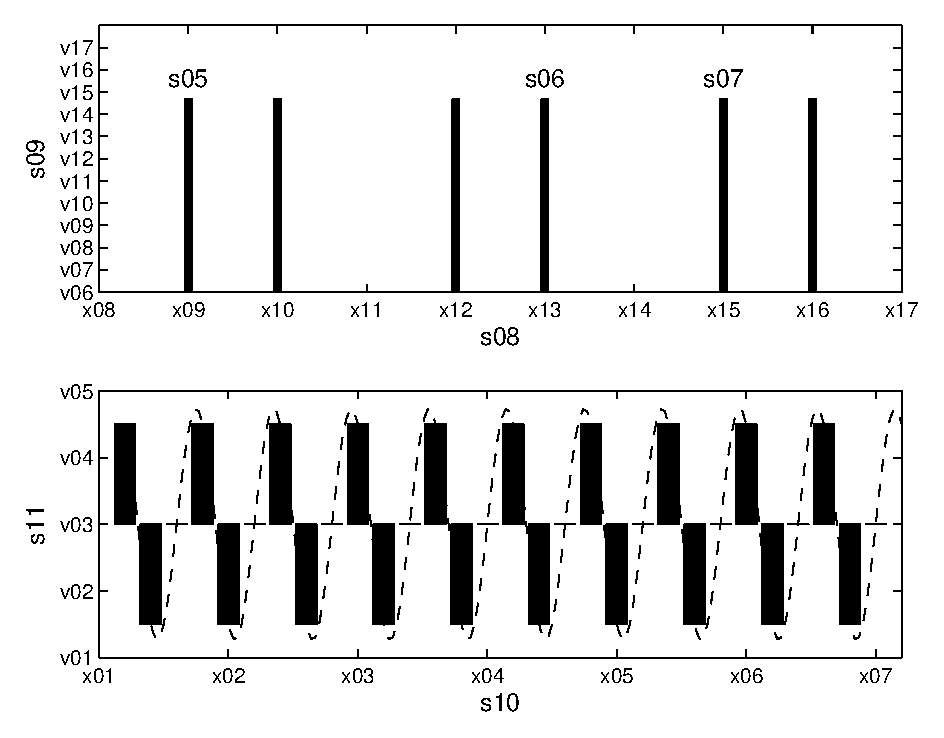
\includegraphics[width=0.47\textwidth]{figs/f_Qs_30_p_10_2.eps}
\end{psfrags}%
%
% End f_Qs_30_p_10_2.tex
\end{document}
% See http://www.mathworks.de/matlabcentral/fileexchange/loadFile.do?objectId=4638
% for recent versions of laprint.m.
%
% created by:           LaPrint version 3.16 (13.9.2004)
% created on:           12-Nov-2008 21:54:09
% eps bounding box:     17.5 cm x 13.125 cm
% comment:              
%
\begin{psfrags}%
\psfragscanon%
%
% text strings:
\psfrag{s05}[b][b]{$\xi_{10}$}
\psfrag{s06}[b][b]{$\xi_{50}$}
\psfrag{s07}[b][b]{$\xi_{70}$}
\psfrag{s08}[t][t]{$\nu$}
\psfrag{s09}[b][b]{$\xi_{\nu}$}
\psfrag{s10}[t][t]{Slot number}
\psfrag{s11}[b][b]{$F_{slot}/\SI{}{A}$}
%
% xticklabels:
\psfrag{x01}[t][t]{0}
\psfrag{x02}[t][t]{5}
\psfrag{x03}[t][t]{10}
\psfrag{x04}[t][t]{15}
\psfrag{x05}[t][t]{20}
\psfrag{x06}[t][t]{25}
\psfrag{x07}[t][t]{30}
\psfrag{x08}[t][t]{0}
\psfrag{x09}[t][t]{10}
\psfrag{x10}[t][t]{20}
\psfrag{x11}[t][t]{30}
\psfrag{x12}[t][t]{40}
\psfrag{x13}[t][t]{50}
\psfrag{x14}[t][t]{60}
\psfrag{x15}[t][t]{70}
\psfrag{x16}[t][t]{80}
\psfrag{x17}[t][t]{90}
%
% yticklabels:
\psfrag{v01}[r][r]{-2}
\psfrag{v02}[r][r]{-1}
\psfrag{v03}[r][r]{0}
\psfrag{v04}[r][r]{1}
\psfrag{v05}[r][r]{2}
\psfrag{v06}[r][r]{0}
\psfrag{v07}[r][r]{0.1}
\psfrag{v08}[r][r]{0.2}
\psfrag{v09}[r][r]{0.3}
\psfrag{v10}[r][r]{0.4}
\psfrag{v11}[r][r]{0.5}
\psfrag{v12}[r][r]{0.6}
\psfrag{v13}[r][r]{0.7}
\psfrag{v14}[r][r]{0.8}
\psfrag{v15}[r][r]{0.9}
\psfrag{v16}[r][r]{1}
\psfrag{v17}[r][r]{1.1}
%
% Figure:
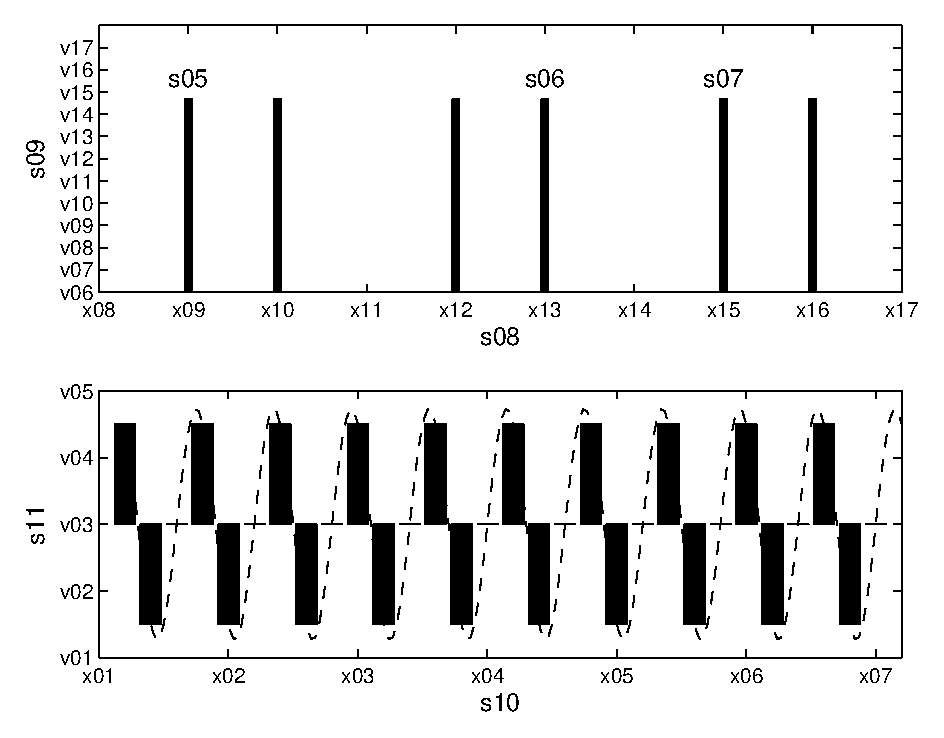
\includegraphics[width=0.47\textwidth]{figs/f_Qs_30_p_10_2.eps}
\end{psfrags}%
%
% End f_Qs_30_p_10_2.tex

	\caption{Non-overlapping double layer winding}
	\label{fig:Main_non-overlapping_double}
\end{figure}

\subsubsection{Single layer overlapping}
A general single layer overlapping winding is shown in~% 
Fig.~\ref{fig:Main_single_overlapping}\subref{fig:slw_yd_eq_1}. In this example the coil pitch equals 5. The ingoing coil side of the first coil is in slot 1 and the outgoing coil side in slot 6. It is clear from the figure that the coils overlap. 

The example to illustrate the slot mmf and current sheet has 30 slots and a pole pair number equal to 5. In Tab.~\ref{tab:Example_table} the average pole pitch equals the pole pitch. Therefore this is called a concentrated winding as determined from Fig.~\ref{fig:classification}. The basic winding matrix elements are given as
\begin{equation}
  \mathbf{M_{1,b}} = 
  \begin{pmatrix}
  1&0&0&-1&0&0\\    
  0&-1&0&0&1&0\\   
  0&0&1&0&0&-1\\   
  \end{pmatrix} \
  \mathbf{M_{2,b}} = 
  \begin{pmatrix}
  1& 0&0&-1&0&0\\
  0&-1&0& 0&1&0\\
  0& 0&1& 0&0&-1\\  
  \end{pmatrix} 
\end{equation}
The calculated winding factor along with the slot mmf and current sheet are shown in Fig.~\ref{fig:Main_single_overlapping}\subref{fig:f_Qs30_5_1}. It is important to mention that the coil sides are distributed in such a way as to obtain a sinusoidal slot mmf distribution. The number of slots per pole and phase can be increased to obtain a better sinusoidal distribution. In doing so, the harmonic content will become less.
\begin{figure}[htbp]
	\centering
	\begin{psfrags}%
\psfragscanon

% text strings:
\psfrag{t01}{{\tiny Coil pitch, $y_d$}}
\psfrag{t02}{{\tiny Overhang, $l_o$}}
\psfrag{t05}{{\tiny 1}}
\psfrag{t06}{{\tiny 2}}
\psfrag{t07}{{\tiny 3}}
\psfrag{t08}{{\tiny 4}}
\psfrag{t09}{{\tiny 5}}
\psfrag{t10}{{\tiny 6}}
\psfrag{t11}{{\tiny Direction of coil assignment}}

% Figure:

\subfloat[Single layer overlapping winding layout\label{fig:slw_yd_eq_1}]{%
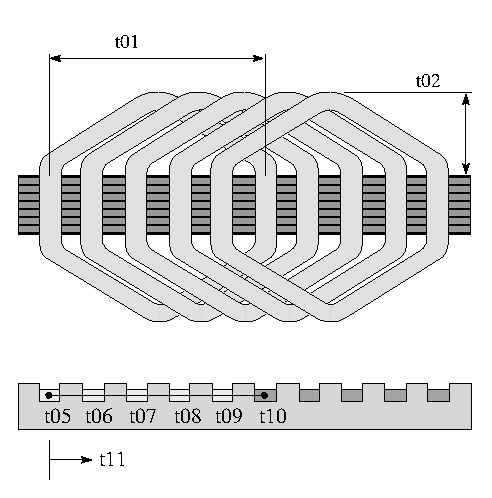
\includegraphics[height=7cm]{figs/f_single_layer_type1.eps}}
\end{psfrags}%
	\vspace{1cm}
	% This file is generated by the MATLAB m-file laprint.m. It can be included
% into LaTeX documents using the packages graphicx, color and psfrag.
% It is accompanied by a postscript file. A sample LaTeX file is:
%    \documentclass{article}\usepackage{graphicx,color,psfrag}
%    \begin{document}% This file is generated by the MATLAB m-file laprint.m. It can be included
% into LaTeX documents using the packages graphicx, color and psfrag.
% It is accompanied by a postscript file. A sample LaTeX file is:
%    \documentclass{article}\usepackage{graphicx,color,psfrag}
%    \begin{document}\input{f_Qs_30_p_5_1}\end{document}
% See http://www.mathworks.de/matlabcentral/fileexchange/loadFile.do?objectId=4638
% for recent versions of laprint.m.
%
% created by:           LaPrint version 3.16 (13.9.2004)
% created on:           12-Nov-2008 21:46:31
% eps bounding box:     17.5 cm x 13.125 cm
% comment:              
%
\begin{psfrags}%
\psfragscanon%
%
% text strings:
\psfrag{s05}[b][b]{$\xi_{5}$}%
\psfrag{s06}[b][b]{$\xi_{25}$}%
\psfrag{s07}[b][b]{$\xi_{35}$}%
\psfrag{s08}[t][t]{$\nu$}%
\psfrag{s09}[b][b]{$\xi_{\nu}$}%
\psfrag{s10}[t][t]{Slot number}%
\psfrag{s11}[b][b]{$F_{slot}/\SI{}{A}$}%
%
% xticklabels:
\psfrag{x01}[t][t]{0}%
\psfrag{x02}[t][t]{5}%
\psfrag{x03}[t][t]{10}%
\psfrag{x04}[t][t]{15}%
\psfrag{x05}[t][t]{20}%
\psfrag{x06}[t][t]{25}%
\psfrag{x07}[t][t]{30}%
\psfrag{x08}[t][t]{0}%
\psfrag{x09}[t][t]{10}%
\psfrag{x10}[t][t]{20}%
\psfrag{x11}[t][t]{30}%
\psfrag{x12}[t][t]{40}%
\psfrag{x13}[t][t]{50}%
\psfrag{x14}[t][t]{60}%
%
% yticklabels:
\psfrag{v01}[r][r]{-1}%
\psfrag{v02}[r][r]{-0.5}%
\psfrag{v03}[r][r]{0}%
\psfrag{v04}[r][r]{0.5}%
\psfrag{v05}[r][r]{1}%
\psfrag{v06}[r][r]{0}%
\psfrag{v07}[r][r]{0.1}%
\psfrag{v08}[r][r]{0.2}%
\psfrag{v09}[r][r]{0.3}%
\psfrag{v10}[r][r]{0.4}%
\psfrag{v11}[r][r]{0.5}%
\psfrag{v12}[r][r]{0.6}%
\psfrag{v13}[r][r]{0.7}%
\psfrag{v14}[r][r]{0.8}%
\psfrag{v15}[r][r]{0.9}%
\psfrag{v16}[r][r]{1}%
\psfrag{v17}[r][r]{1.1}%
%
% Figure:

\subfloat[Slot mmf and winding factors\label{fig:f_Qs30_5_1}]{%
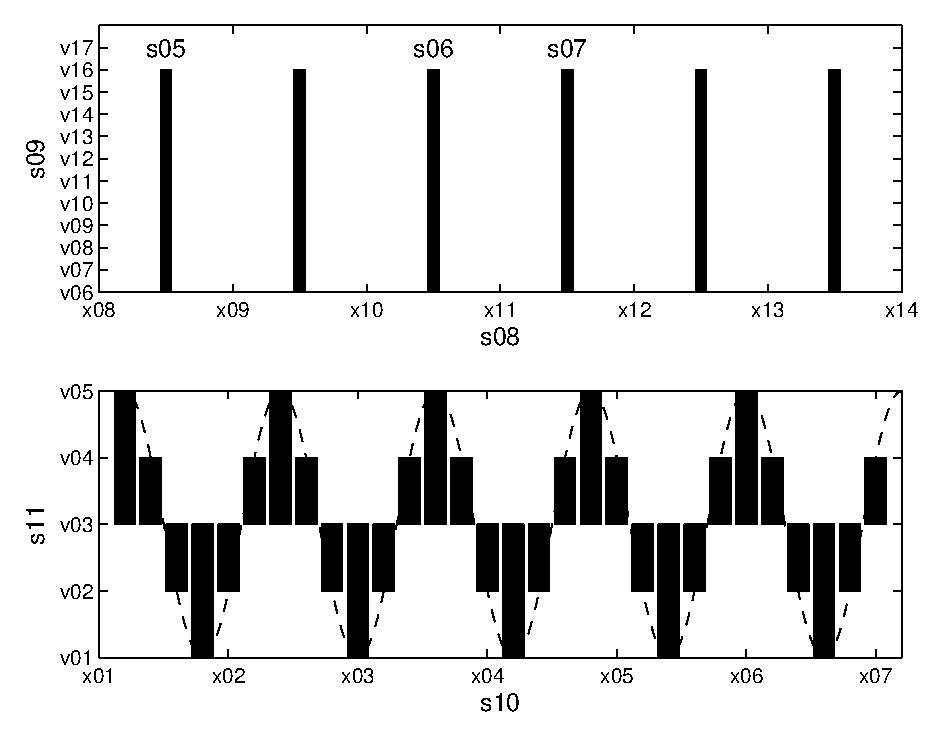
\includegraphics[width=0.9\textwidth]{figs/f_Qs_30_p_5_1.eps}}%
\end{psfrags}%
%
% End f_Qs_30_p_5_1.tex
\end{document}
% See http://www.mathworks.de/matlabcentral/fileexchange/loadFile.do?objectId=4638
% for recent versions of laprint.m.
%
% created by:           LaPrint version 3.16 (13.9.2004)
% created on:           12-Nov-2008 21:46:31
% eps bounding box:     17.5 cm x 13.125 cm
% comment:              
%
\begin{psfrags}%
\psfragscanon%
%
% text strings:
\psfrag{s05}[b][b]{$\xi_{5}$}%
\psfrag{s06}[b][b]{$\xi_{25}$}%
\psfrag{s07}[b][b]{$\xi_{35}$}%
\psfrag{s08}[t][t]{$\nu$}%
\psfrag{s09}[b][b]{$\xi_{\nu}$}%
\psfrag{s10}[t][t]{Slot number}%
\psfrag{s11}[b][b]{$F_{slot}/\SI{}{A}$}%
%
% xticklabels:
\psfrag{x01}[t][t]{0}%
\psfrag{x02}[t][t]{5}%
\psfrag{x03}[t][t]{10}%
\psfrag{x04}[t][t]{15}%
\psfrag{x05}[t][t]{20}%
\psfrag{x06}[t][t]{25}%
\psfrag{x07}[t][t]{30}%
\psfrag{x08}[t][t]{0}%
\psfrag{x09}[t][t]{10}%
\psfrag{x10}[t][t]{20}%
\psfrag{x11}[t][t]{30}%
\psfrag{x12}[t][t]{40}%
\psfrag{x13}[t][t]{50}%
\psfrag{x14}[t][t]{60}%
%
% yticklabels:
\psfrag{v01}[r][r]{-1}%
\psfrag{v02}[r][r]{-0.5}%
\psfrag{v03}[r][r]{0}%
\psfrag{v04}[r][r]{0.5}%
\psfrag{v05}[r][r]{1}%
\psfrag{v06}[r][r]{0}%
\psfrag{v07}[r][r]{0.1}%
\psfrag{v08}[r][r]{0.2}%
\psfrag{v09}[r][r]{0.3}%
\psfrag{v10}[r][r]{0.4}%
\psfrag{v11}[r][r]{0.5}%
\psfrag{v12}[r][r]{0.6}%
\psfrag{v13}[r][r]{0.7}%
\psfrag{v14}[r][r]{0.8}%
\psfrag{v15}[r][r]{0.9}%
\psfrag{v16}[r][r]{1}%
\psfrag{v17}[r][r]{1.1}%
%
% Figure:

\subfloat[Slot mmf and winding factors\label{fig:f_Qs30_5_1}]{%
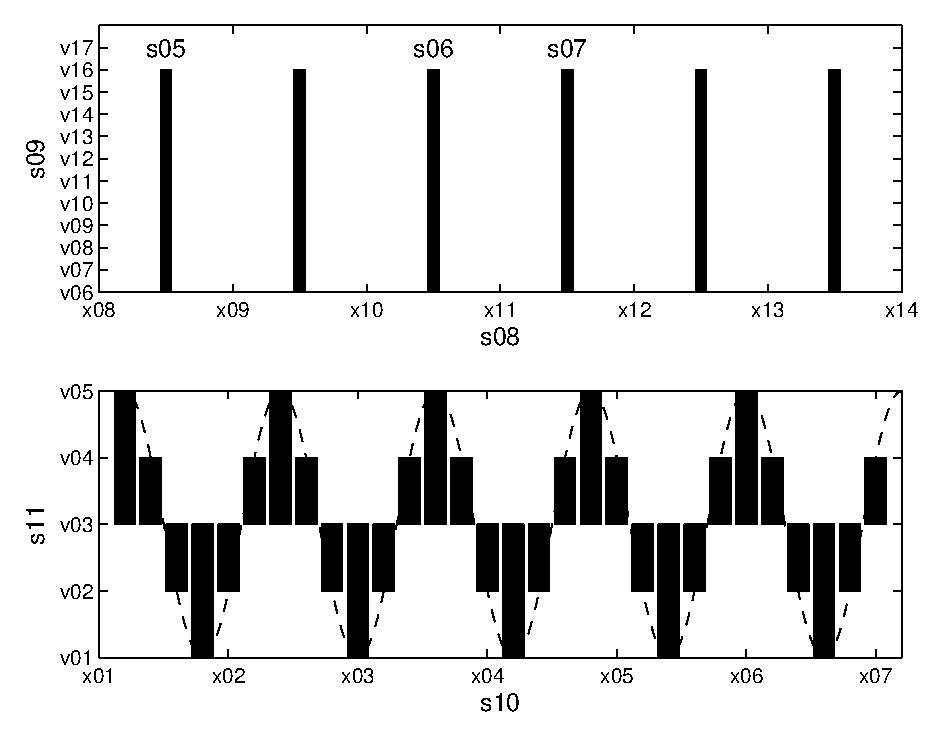
\includegraphics[width=0.9\textwidth]{figs/f_Qs_30_p_5_1.eps}}%
\end{psfrags}%
%
% End f_Qs_30_p_5_1.tex

	\caption{Single layer overlapping winding}
	\label{fig:Main_single_overlapping}
\end{figure}

\subsubsection{Double layer overlapping}
A double layer overlapping winding is commonly used in industrial machines. Overlapping double layer windings have a coil pitch greater than one, i.e.~$y_d>1$. Fig.~\ref{fig:dlw_yd_gt_1} shows a double layer winding. Starting at the first slot, the coils are inserted in a counter-clockwise direction. The first coil has its ingoing coil side in the bottom part of slot 1 and the return coil side is in the top part of slot 6. The phase belt constraint in \eqref{eqn:phase_belt_constraint} is used to determine the phase of the coil side in the bottom part of the slot while the top coil sides are given by the coil pitch $y_d$.

Fig.~\ref{fig:f_Qs30_p5_2} shows the slot mmf of a stator with $Q_s=30$ slots and $p=5$ pole pairs. Using the winding properties for this combination given in Tab.~\ref{tab:Example_table}, it is a concentrated winding. The winding has no sub-harmonics. 
\begin{figure}[htbp]
	\centering
	\begin{psfrags}%
\psfragscanon

% text strings:
\psfrag{t01}{{\tiny Coil pitch, $y_d$}}
\psfrag{t02}{{\tiny Overhang, $l_o$}}
\psfrag{t03}{{\tiny Top}}
\psfrag{t04}{{\tiny Bottom}}
\psfrag{t05}{{\tiny 1}}
\psfrag{t06}{{\tiny 2}}
\psfrag{t07}{{\tiny 3}}
\psfrag{t08}{{\tiny 4}}
\psfrag{t09}{{\tiny 5}}
\psfrag{t10}{{\tiny 6}}
\psfrag{t11}{{\tiny Direction of coil assignment}}


% Figure:

\subfloat[Double layer overlapping winding layout\label{fig:dlw_yd_gt_1}]{%
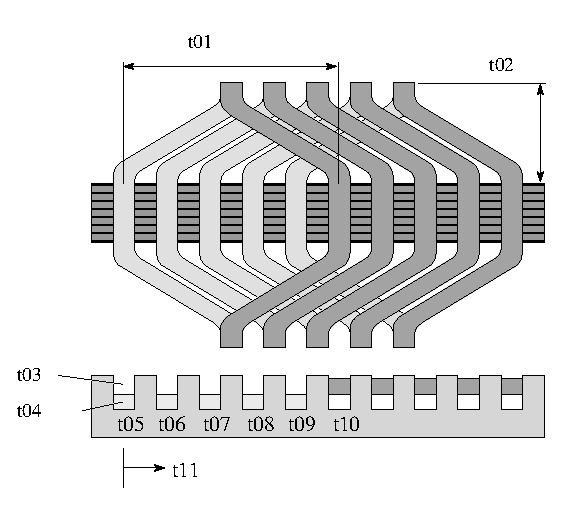
\includegraphics[height=7cm]{figs/f_double_layer.eps}}
\end{psfrags}%
	\vspace{1cm}
	% This file is generated by the MATLAB m-file laprint.m. It can be included
% into LaTeX documents using the packages graphicx, color and psfrag.
% It is accompanied by a postscript file. A sample LaTeX file is:
%    \documentclass{article}\usepackage{graphicx,color,psfrag}
%    \begin{document}% This file is generated by the MATLAB m-file laprint.m. It can be included
% into LaTeX documents using the packages graphicx, color and psfrag.
% It is accompanied by a postscript file. A sample LaTeX file is:
%    \documentclass{article}\usepackage{graphicx,color,psfrag}
%    \begin{document}\input{f_Qs_30_p_5_2}\end{document}
% See http://www.mathworks.de/matlabcentral/fileexchange/loadFile.do?objectId=4638
% for recent versions of laprint.m.
%
% created by:           LaPrint version 3.16 (13.9.2004)
% created on:           12-Nov-2008 21:50:28
% eps bounding box:     17.5 cm x 13.125 cm
% comment:              
%
\begin{psfrags}%
\psfragscanon%
%
% text strings:
\psfrag{s05}[b][b]{{\tiny $\xi_{5}$}}%
\psfrag{s06}[b][b]{{\tiny $\xi_{25}$}}%
\psfrag{s07}[b][b]{{\tiny $\xi_{35}$}}%
\psfrag{s08}[t][t]{{\tiny $\nu$}}%
\psfrag{s09}[b][b]{{\tiny $\xi_{\nu}$}}%
\psfrag{s10}[t][t]{{\tiny Slot number}}%
\psfrag{s11}[b][b]{{\tiny $F_{slot}/\SI{}{A}$}}%
%
% xticklabels:
\psfrag{x01}[t][t]{{\tiny 0}}%
\psfrag{x02}[t][t]{{\tiny 5}}%
\psfrag{x03}[t][t]{{\tiny 10}}%
\psfrag{x04}[t][t]{{\tiny 15}}%
\psfrag{x05}[t][t]{{\tiny 20}}%
\psfrag{x06}[t][t]{{\tiny 25}}%
\psfrag{x07}[t][t]{{\tiny 30}}%
\psfrag{x08}[t][t]{{\tiny 0}}%
\psfrag{x09}[t][t]{{\tiny 10}}%
\psfrag{x10}[t][t]{{\tiny 20}}%
\psfrag{x11}[t][t]{{\tiny 30}}%
\psfrag{x12}[t][t]{{\tiny 40}}%
\psfrag{x13}[t][t]{{\tiny 50}}%
\psfrag{x14}[t][t]{{\tiny 60}}%
%
% yticklabels:
\psfrag{v01}[r][r]{{\tiny -2}}%
\psfrag{v02}[r][r]{{\tiny -1}}%
\psfrag{v03}[r][r]{{\tiny 0}}%
\psfrag{v04}[r][r]{{\tiny 1}}%
\psfrag{v05}[r][r]{{\tiny 2}}%
\psfrag{v06}[r][r]{{\tiny 0}}%
\psfrag{v07}[r][r]{{\tiny 0.1}}%
\psfrag{v08}[r][r]{{\tiny 0.2}}%
\psfrag{v09}[r][r]{{\tiny 0.3}}%
\psfrag{v10}[r][r]{{\tiny 0.4}}%
\psfrag{v11}[r][r]{{\tiny 0.5}}%
\psfrag{v12}[r][r]{{\tiny 0.6}}%
\psfrag{v13}[r][r]{{\tiny 0.7}}%
\psfrag{v14}[r][r]{{\tiny 0.8}}%
\psfrag{v15}[r][r]{{\tiny 0.9}}%
\psfrag{v16}[r][r]{{\tiny 1}}%
\psfrag{v17}[r][r]{{\tiny 1.1}}%
%
% Figure:

\subfloat[Slot mmf and winding factors\label{fig:f_Qs30_p5_2}]{%
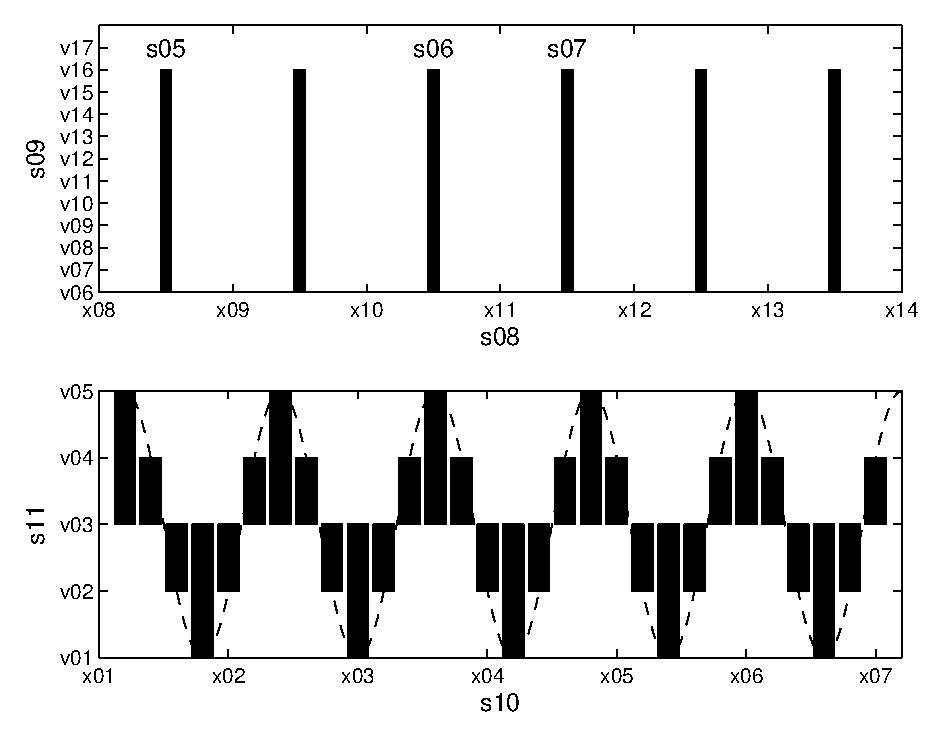
\includegraphics[width=0.9\textwidth]{figs/f_Qs_30_p_5_2.eps}}%
\end{psfrags}%
%
% End f_Qs_30_p_5_2.tex
\end{document}
% See http://www.mathworks.de/matlabcentral/fileexchange/loadFile.do?objectId=4638
% for recent versions of laprint.m.
%
% created by:           LaPrint version 3.16 (13.9.2004)
% created on:           12-Nov-2008 21:50:28
% eps bounding box:     17.5 cm x 13.125 cm
% comment:              
%
\begin{psfrags}%
\psfragscanon%
%
% text strings:
\psfrag{s05}[b][b]{{\tiny $\xi_{5}$}}%
\psfrag{s06}[b][b]{{\tiny $\xi_{25}$}}%
\psfrag{s07}[b][b]{{\tiny $\xi_{35}$}}%
\psfrag{s08}[t][t]{{\tiny $\nu$}}%
\psfrag{s09}[b][b]{{\tiny $\xi_{\nu}$}}%
\psfrag{s10}[t][t]{{\tiny Slot number}}%
\psfrag{s11}[b][b]{{\tiny $F_{slot}/\SI{}{A}$}}%
%
% xticklabels:
\psfrag{x01}[t][t]{{\tiny 0}}%
\psfrag{x02}[t][t]{{\tiny 5}}%
\psfrag{x03}[t][t]{{\tiny 10}}%
\psfrag{x04}[t][t]{{\tiny 15}}%
\psfrag{x05}[t][t]{{\tiny 20}}%
\psfrag{x06}[t][t]{{\tiny 25}}%
\psfrag{x07}[t][t]{{\tiny 30}}%
\psfrag{x08}[t][t]{{\tiny 0}}%
\psfrag{x09}[t][t]{{\tiny 10}}%
\psfrag{x10}[t][t]{{\tiny 20}}%
\psfrag{x11}[t][t]{{\tiny 30}}%
\psfrag{x12}[t][t]{{\tiny 40}}%
\psfrag{x13}[t][t]{{\tiny 50}}%
\psfrag{x14}[t][t]{{\tiny 60}}%
%
% yticklabels:
\psfrag{v01}[r][r]{{\tiny -2}}%
\psfrag{v02}[r][r]{{\tiny -1}}%
\psfrag{v03}[r][r]{{\tiny 0}}%
\psfrag{v04}[r][r]{{\tiny 1}}%
\psfrag{v05}[r][r]{{\tiny 2}}%
\psfrag{v06}[r][r]{{\tiny 0}}%
\psfrag{v07}[r][r]{{\tiny 0.1}}%
\psfrag{v08}[r][r]{{\tiny 0.2}}%
\psfrag{v09}[r][r]{{\tiny 0.3}}%
\psfrag{v10}[r][r]{{\tiny 0.4}}%
\psfrag{v11}[r][r]{{\tiny 0.5}}%
\psfrag{v12}[r][r]{{\tiny 0.6}}%
\psfrag{v13}[r][r]{{\tiny 0.7}}%
\psfrag{v14}[r][r]{{\tiny 0.8}}%
\psfrag{v15}[r][r]{{\tiny 0.9}}%
\psfrag{v16}[r][r]{{\tiny 1}}%
\psfrag{v17}[r][r]{{\tiny 1.1}}%
%
% Figure:

\subfloat[Slot mmf and winding factors\label{fig:f_Qs30_p5_2}]{%
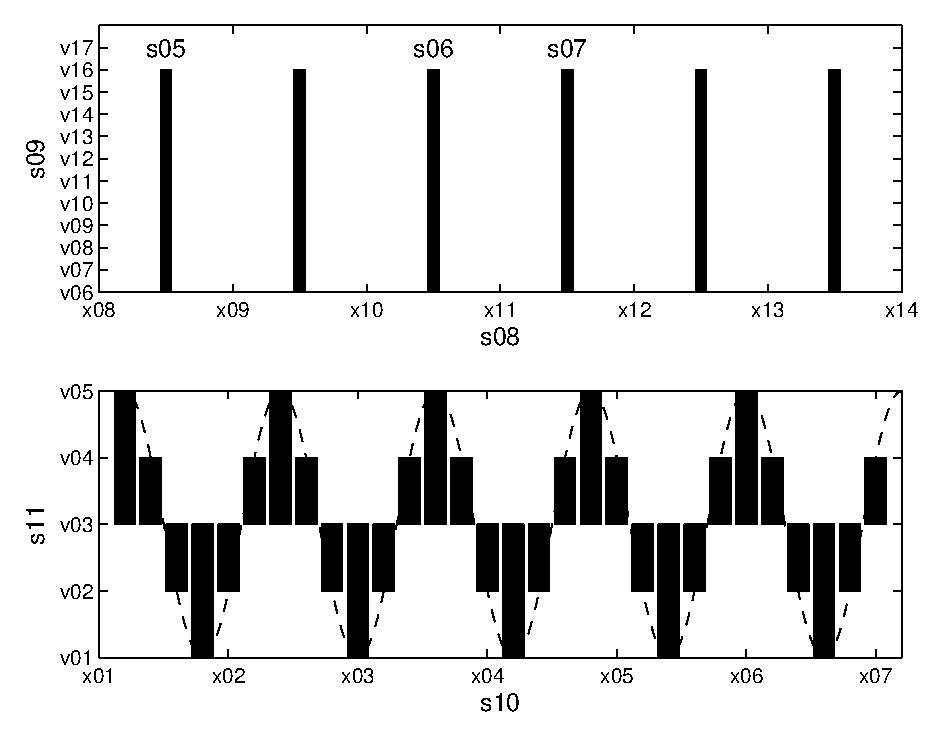
\includegraphics[width=0.9\textwidth]{figs/f_Qs_30_p_5_2.eps}}%
\end{psfrags}%
%
% End f_Qs_30_p_5_2.tex

	\caption{Double layer overlapping winding}
	\label{Main_double_overlapping}
\end{figure}

\section{Determination of the winding axes}\label{sec:axes}
The winding axes are determined for the prototype with 30 slots and 10 pole pairs. Since the winding factor is a complex number, the winding factor of the working harmonic is calculated using \eqref{eqn:winding_factor}, i.e. 
\begin{equation}
  \xi_{10} = 0.7500 + j0.4330
  \quad
  \begin{cases}
  a_{10} = 0.7500\\
  b_{10} = 0.4330\\
  \left|\xi_{10}\right|=0.866\\
  \arctan\left(\frac{b_{10}}{a_{10}}\right)=0.5236
  \end{cases}
\end{equation}
Fig.~\ref{fig:determ_axis} graphically shows the current sheet anti-node and magnetic axes. The axes were calculated using a stator slot with regular distributed stator slots. The calculated angles are given in terms of the first slot. 
\begin{figure}
	\centering
		\begin{psfrags}%
\psfragscanon%
%
% text strings:
\psfrag{t01}[bl]{\tiny{$x$}}%
\psfrag{t02}[bl]{\tiny{$y$}}%
\psfrag{t03}[bc]{\tiny{$0^{\circ}$}}%
\psfrag{t04}[bl]{\tiny{Current sheet}}%
\psfrag{t05}[bl]{\tiny{$-3^{\circ}$}}%
\psfrag{t06}[bl]{\tiny{Magnetic axis $\left(\theta_{m}\right)$}}%
\psfrag{t07}[bl]{\tiny{$-9^{\circ}$}}%
\psfrag{t08}[bl]{\tiny{$48^{\circ}$}}%
\psfrag{t09}[bl]{\tiny{$57^{\circ}$}}%
\psfrag{t10}[bl]{\tiny{$72^{\circ}$}}%
\psfrag{t11}[bl]{\tiny{$54^{\circ}$}}%
\psfrag{t12}[bl]{\tiny{anti-node axis $\left(\theta_{an}\right)$}}%

%
% Figure:
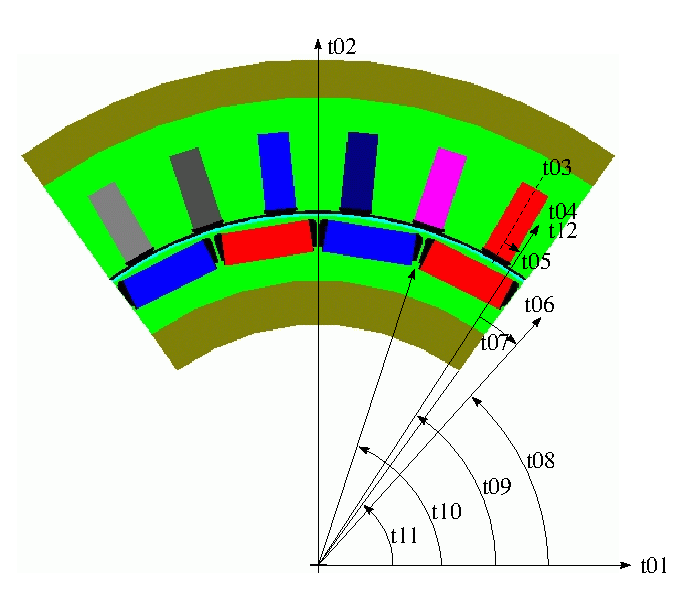
\includegraphics[width=0.9\textwidth]{figs/ch3/f_axis.eps}%
\end{psfrags}

	\caption{Determination of the winding axes}
	\label{fig:determ_axis}
\end{figure}

\section{Summary}
In this chapter an algorithm was derived to present a winding in a matrix form. This compact form allows the calculation of the winding factors for all harmonics. The basis of the algorithm is the phase belt sequence and the phase belt constraint which are derived from the air gap mmf envelope functions. The chapter was concluded with  examples which showed how the winding matrix can be used to calculate the slot mmf and the winding axes. This answers the research sub-questions.

In the next chapter the properties of the materials used in the finite element method are given. This is necessary to correctly model the material data supplied by the manufacturer. In addition, the basic equations are explained to calculate the machine's flux linkages and inductances.    

\endinput
\chapter{Nonlinear magnetic circuit analysis}\label{chap:NonlinearAnalysis}
Due to the nonlinear material behaviour a nonlinear magnetic circuit analysis needs to be carried out in order to determine the machine performance. The nonlinear material properties and the solutions to the nonlinear machine behaviour are the main themes of this chapter. Additionally, the chapter concludes with practical guidelines for a harmonic analysis.

\section{Introductory remarks}
One aspect in the main research question is the accuracy of the calculated machine performance. For high accuracy it is necessary to perform a nonlinear magnetic circuit analysis. Since the nonlinear machine behaviour arises from the materials, it is appropriate to have a detailed knowledge of the material data. 

The machine performance is calculated using the finite element method. In most documentation the terms \emph{finite element method} and \emph{finite element analysis} seem to be used interchangeably. There is, however, a small difference between the terms:
\begin{description}
	\item[The finite element method] is a numerical technique for finding approximate solutions to ordinary and elliptic partial differential equations via a piecewise polynomial interpolation scheme. There are essentially three mathematical ways that FEM can evaluate the values at the nodes: the non-variational method (Ritz), the residual method (Galerkin), and the variational method (Rayleigh-Ritz).
	\item[Finite element analysis] is an implementation of FEM to solve a certain type of problem. In the case of electrical machines the most common solution type is a 2D magnetostatic problem. Typically the residual method is used to obtain the FEM mathematical solution and a suitable element type is needed for the analysis. The software used in the present dissertation makes use of first order triangular elements. 
\end{description}

The machine's performance calculations in the analysis of interior permanent magnet machines with non-overlapping concentrated windings are based mainly on the fundamental quantities. In order to get the fundamental quantities, and especially in the case of a spatial harmonic analysis, the discrete Fourier transform is used.

\section{Material properties} \label{sec:mat_properties}
In the context of electrical machines the importance of magnetic materials is twofold. Through their use it is possible to obtain large flux densities with relatively low levels of magnetisation. In addition, and especially in machines, the laminated steel is used to constrain and direct magnetic fields in well defined paths. The magnetic materials are used to shape the fields to maximise the desired torque producing characteristics. Therefore a knowledgeable design engineer can make use of the material properties to achieve specific desirable results.  

\subsection{Laminated steel}
Obtaining meaningful loss results in machine design requires accurate representation of the material properties. The saturation level in machines is often beyond the measured data supplied by the manufactures. This means that it is necessary to extrapolate the data. Typically the supplied magnetic polarisation $J$ is in the range from \SI{1.5}{T} to \SI{1.8}{T}, whereas the flux density $B$ in the teeth could be up to \SI{2.1}{T}. In order to calculate flux densities above \SI{2}{T} the following steps need to be taken:
\begin{itemize*}
	\item the magnetic polarisation needs to be extrapolated to its saturation~%
	value $J_s$; and
	\item the magnetic polarisation needs to be converted to the flux density.
\end{itemize*}
The manner in which these two steps are executed will influence the method or way to determine the so-called correction factors for the iron loss. It is important to mention that the iron loss calculations are strongly influenced by the manufacturing process. Once the laminations are punched or lasered the material properties change and lead to higher losses.  

\subsubsection{Epstein frame measurements}
An Epstein frame is a standardised measurement device for measuring the magnetic properties of soft magnetic materials and especially that of the laminations used in electrical machines. The main properties measured are the polarisation and the specific loss. Fig.~\ref{fig:epstein_frame}(a) shows the measurement setup used to measure the polarisation and specific loss for M470P65A lamination steel. The test sample is prepared as a set consisting of a number of strips. The specimen is then arranged in the Epstein frame as shown in Fig.~\ref{fig:epstein_frame}(b).  
\begin{figure}[htbp]
	\centering
		\input{figs/ch4/f_epstein.tex}
		\caption{Measurement setup to measure $J(H)$ for laminated steel}
		\label{fig:epstein_frame}
\end{figure}

The relationship between $J$ and $H$ for laminated steel is both nonlinear and multivalued. In general, the characteristics of the material cannot be described analytically. They are commonly presented in graphical form or a set of data points. Fig.~\ref{fig:Main_M470P65A}\subref{fig:JH_M470_zoom} shows a graphical presentation of the measured polarisation for M470P65A laminated steel for frequencies in the range \SI{50}{Hz} to \SI{120}{Hz}. From the measured results the frequency dependency of lamination steel comes to the fore.

The second measurement that the Epstein frame is used for is the specific loss. For the specific loss measurement the strips need to be weighed using an accurate scale. Measured results for the specific loss in the range from \SI{50}{Hz} to \SI{120}{Hz} are shown in Fig.~\ref{fig:Main_M470P65A}\subref{fig:P_M470_3D}. The specific loss has a dependency on both the frequency and polarisation. The two-dimensional presentation of the data is not typical, but emphasises the nonlinear and multivalued properties.
\begin{figure}[htbp]
  \centering
  % This file is generated by the MATLAB m-file laprint.m. It can be included
% into LaTeX documents using the packages graphicx, color and psfrag.
% It is accompanied by a postscript file. A sample LaTeX file is:
%    \documentclass{article}\usepackage{graphicx,color,psfrag}
%    \begin{document}% This file is generated by the MATLAB m-file laprint.m. It can be included
% into LaTeX documents using the packages graphicx, color and psfrag.
% It is accompanied by a postscript file. A sample LaTeX file is:
%    \documentclass{article}\usepackage{graphicx,color,psfrag}
%    \begin{document}\input{f_dependancy}\end{document}
% See http://www.mathworks.de/matlabcentral/fileexchange/loadFile.do?objectId=4638
% for recent versions of laprint.m.
%
% created by:           LaPrint version 3.16 (13.9.2004)
% created on:           14-Sep-2008 12:31:21
% eps bounding box:     7.5 cm x 5.625 cm
% comment:              
%
\begin{psfrags}%
\psfragscanon%
%
% text strings:
\psfrag{s03}[t][t]{{\tiny $H/\SI{}{A.m^{-1}}$}}%
\psfrag{s04}[b][b]{{\tiny $J/\SI{}{T}$}}%
\psfrag{s05}[bl]{{\tiny \SI{120}{Hz}}}%
\psfrag{s06}[br]{{\tiny \SI{50}{Hz}}}%
%
% xticklabels:
\psfrag{x01}[t][t]{{\tiny $10^{2}$}}%
%
% yticklabels:
\psfrag{v01}[r][r]{{\tiny 0}}%
\psfrag{v02}[r][r]{{\tiny 0.2}}%
\psfrag{v03}[r][r]{{\tiny 0.4}}%
\psfrag{v04}[r][r]{{\tiny 0.6}}%
\psfrag{v05}[r][r]{{\tiny 0.8}}%
\psfrag{v06}[r][r]{{\tiny 1}}%
\psfrag{v07}[r][r]{{\tiny 1.2}}%
\psfrag{v08}[r][r]{{\tiny 1.4}}%
%
% Figure:
%\includegraphics[width=0.7\textwidth]{figs/ch4/f_dependancy.eps}%

\subfloat[Frequency dependency of $J(H)$\label{fig:JH_M470_zoom}]{%
\includegraphics[height=8cm]{figs/ch4/f_dependancy.eps}}%
\end{psfrags}%
\end{document}
% See http://www.mathworks.de/matlabcentral/fileexchange/loadFile.do?objectId=4638
% for recent versions of laprint.m.
%
% created by:           LaPrint version 3.16 (13.9.2004)
% created on:           14-Sep-2008 12:31:21
% eps bounding box:     7.5 cm x 5.625 cm
% comment:              
%
\begin{psfrags}%
\psfragscanon%
%
% text strings:
\psfrag{s03}[t][t]{{\tiny $H/\SI{}{A.m^{-1}}$}}%
\psfrag{s04}[b][b]{{\tiny $J/\SI{}{T}$}}%
\psfrag{s05}[bl]{{\tiny \SI{120}{Hz}}}%
\psfrag{s06}[br]{{\tiny \SI{50}{Hz}}}%
%
% xticklabels:
\psfrag{x01}[t][t]{{\tiny $10^{2}$}}%
%
% yticklabels:
\psfrag{v01}[r][r]{{\tiny 0}}%
\psfrag{v02}[r][r]{{\tiny 0.2}}%
\psfrag{v03}[r][r]{{\tiny 0.4}}%
\psfrag{v04}[r][r]{{\tiny 0.6}}%
\psfrag{v05}[r][r]{{\tiny 0.8}}%
\psfrag{v06}[r][r]{{\tiny 1}}%
\psfrag{v07}[r][r]{{\tiny 1.2}}%
\psfrag{v08}[r][r]{{\tiny 1.4}}%
%
% Figure:
%\includegraphics[width=0.7\textwidth]{figs/ch4/f_dependancy.eps}%

\subfloat[Frequency dependency of $J(H)$\label{fig:JH_M470_zoom}]{%
\includegraphics[height=8cm]{figs/ch4/f_dependancy.eps}}%
\end{psfrags}%
 
  \vspace{1cm}
  \input{figs/ch4/f_specific_P.tex} 
  \caption{The measured data for M470P65A lamination steel}
  \label{fig:Main_M470P65A}
\end{figure}

\subsubsection{Extrapolation of the \textit{B(H)} Curve}\label{sec:extrapolation}
Manufacturers of laminated steel usually provide $J(H)$ data but this data may be defined only partly through to the knee point of the curve. For accurate FEA results the $J(H)$ curve needs to be defined well into the saturation region. Above the knee the slope $\frac{dJ}{dH}$ approaches zero when $J$ is plotted against $H$ as $H$ increases indefinitely. The curve conforms more or less to the Fr�hlich-Kennelly relation as explained in the book by \cite{Bozorth1993}, i.e.
\begin{equation}\label{i_mu}
  \frac{1}{\mu} = a + bH \quad \left(\mu=\mu_0 \mu_r \right)
\end{equation} 
and the saturation polarisation is then calculated as 
\begin{equation}
  J_{s}=\frac{1}{a}
\end{equation} 
In practical engineering problems it is preferred to use $B$ instead of $J$. The flux density and magnetic polarisation have the following relationship: 
\begin{equation}\label{B}
  B = \mu_{0}H + J
\end{equation}
Equation \eqref{B} adapt the so-called Kennelly convention given in \cite{bertotti_1988}. Here the magnetic polarisation $M$ is used in its alternative form. In the SI system of units the magnetic quantities are related as follows:
\begin{align}\label{B_gen}
  B = \mu_{0}\left(H + M\right)
\end{align}
Using \eqref{i_mu} and \eqref{B} the $B(H)$ curve can be defined well into the saturation. The material coefficients for M470P65A laminated steel supplied by the manufacturer together with the extrapolation and conversion for M470P65A are shown graphically in Fig.~\ref{fig:bh_curve_M470}. The saturation polarisation $J_s=2.064$ and the coefficients $a$ and $b$ equal \num{0.484} and \num{779.3} respectively.
\begin{figure}[htbp]
	\centering
	\input{figs/ch4/f_extra_BH.tex}
	\caption{The extrapolation of the $B(H)$ for M470P65A lamination steel}
	\label{fig:bh_curve_M470}
\end{figure}

If the $J_{s}$ is not supplied it could be calculated using \eqref{i_mu}. In order to do so the last two measured points from supplier $J(H)$ curve are used. If $J_1<J_2$, the coefficients $a$ and $b$ can then be obtained by solving two simultaneous equations, i.e. 
\begin{equation}
  \left.
  \begin{aligned}
    \frac{1}{\mu} &= a + bH_1 \\
    \frac{1}{\mu} &= a + bH_2
  \end{aligned}
  \right\}
  \quad
  \mu = \frac{J_2 - J_1}{H_2 - H_1}
\end{equation}

\subsubsection{Three-term core loss model}
The iron losses are linked with the magnetisation process and consists of three parts. The so-called separation of losses implies that the average power loss per unit volume of any material is decomposed into the sum of hysteresis and a dynamic contribution. For several alloys and sinusoidal excitation, with a given frequency and magnetisation, \cite{bertotti_1988} showed that the specific loss is expressed as the sum of the hysteresis $P_{h}$, classical eddy current $P_{c}$ and excess loss $P_{e}$, i.e. 
\begin{equation}
  \label{pfe_bertotti}
  \begin{aligned}
  p_{Fe} &= P_{h} + P_{c} + P_{e}   \\
         &= k_{h}fJ^{2} + k_{c}\left(fJ\right)^{2} + 
         k_{e}\left(fJ\right)^{1.5}
  \end{aligned}
\end{equation}

The specific loss is a function of two variables and it is required to find the unknown  coefficients in \eqref{pfe_bertotti}. The coefficients can be extracted over a family of core loss curves at various frequencies. With the coefficients $k_{h}$, $k_{c}$, and $k_{e}$ the total core loss per unit volume $p_{Fe}$ can be calculated in terms of the peak magnetic polarisation $J$ and the frequency.

The specific loss $p_{Fe}$ as given in \eqref{pfe_bertotti} is a multivariate model with two independent variables. In practical machine design, the unknown coefficients are determined for a given polarisation. Therefore the specific loss becomes a function of frequency and the measured data are used to form a set of $n$ simultaneous equations, i.e. 
\begin{equation}
  p_i = f_{i}J^2 + (f_{i}J)^2 + (f_{i}J)^{1.5} 
  \quad 
  \begin{cases}
  1\leq i \leq n\\
  n\geq3 \\
  \end{cases}
\end{equation}
In order to solve the set of simultaneous equations, it is necessary to construct the regression matrix $\mathbf{X}$ as follows:
\begin{equation}
  \label{eqn:regression}
  \begin{aligned}
  \left[
  \begin{array}{c}
     p_{1}\\
     p_{2}\\
     \vdots\\
     p_{n}\\
  \end{array} \right]&=\left[
  \begin{array}{c c c}
     f_{1}J^2 & (f_{1}J)^2 & (f_{1}J)^{1.5}\\
     f_{2}J^2 & (f_{2}J)^2 & (f_{2}J)^{1.5}\\
     \vdots\\
     f_{n}J^2 & (f_{n}J)^2 & (f_{n}J)^{1.5}\\
  \end{array} \right]\left[
  \begin{array}{c}
     k_h\\
     k_c\\
     k_e
  \end{array} \right]\\ \: \\
  \mathbf{p} &= \mathbf{X}\mathbf{k}
  \end{aligned}
\end{equation}
The unknown coefficients are solved by performing a least squares fit to the regression equation in \eqref{pfe_bertotti}. This method is the easiest and does not take into account any constraints.

\cite{bertotti_1988} explains in his paper that $k_c$ is a fixed value and can be expressed as
\begin{equation}
  k_c = \frac{\pi^{2} \sigma d^{2}}{6}
\end{equation} 
where $\sigma$ is the conductivity and $d$ the lamination thickness. If $k_c$ is a constant it means that only $k_h$ and $k_e$ need to be determined. Using the model in \eqref{pfe_bertotti} often results in negative values for $k_e$. A negative value for $k_e$ has no physical sense. 

Another way to show this inconsistency is to calculate the coefficients without any constraint on $k_c$. A regression matrix is formed for each of the polarisation values given in Tab.~\ref{tab:MultipleRegressionResults}. The calculated coefficients for the different polarisation values are given in the corresponding columns. To validate the model, the maximum of the absolute value of the deviation of the data from the model $e_{max}$ is given. In each case this is sufficiently small to be confident that the model reasonably fits the data.
\begin{table}[htbp]
  \centering
  \caption{Multiple regression results for M470P65A lamination steel}
  \begin{tabular}{lccccccc}
		\toprule
    $J$/\SI{}{T}& \num{0.25}  & \num{1.55}  & \num{1.60}   & \num{1.65}   & \num{1.70}%
             & \num{1.75}   & \num{1.80}   \\
    \hline
    $k_h$  & \num{0.0712} & \num{0.0019} & \num{0.0017} & \num{0.0016} & \num{0.0015}%
         & \num{0.0015} & \num{0.0013}\\
    \hline
    $k_c$  & \num{0.0004} & \num{0.0000} & \num{0.0000} & \num{0.0000} & \num{0.0000}%
         & \num{0.0000} & \num{0.0000}\\
    \hline
    $k_e$  & \num{0.0053} & \num{0.0003} & \num{0.0003} & \num{0.0003} & \num{0.0003}%
         & \num{0.0003} & \num{0.0003}\\
    \hline
    $e_{max}/\SI{}{W.kg^{-1}}$&\num{0.0014} &\num{0.0010}& \num{0.0009} & \num{0.0008}%
           & \num{0.0008} & \num{0.0009} & \num{0.0009}\\
    \bottomrule	
	\end{tabular}
	\label{tab:MultipleRegressionResults}
\end{table}
As the polarisation is increased, the coefficient $k_c$ becomes zero. This inconstancy means that the material characteristics cannot be uniquely described analytically. \cite{Neuschl2007} came to the conclusion that, independent of the analytical method used, there is always a difference between the measured and calculated iron loss. \cite{Chen2002} explained in their paper that there is a big discrepancy between the calculation based on \cite{bertotti_1988} and experimental results if the polarisation is over \SI{1}{T} or if the field frequency becomes high. To overcome this discrepancy they have proposed a new modified formula to represent the coefficient changes. 

\subsubsection{Two-term core loss model}
Even though \cite{bertotti_1988} presented a three-term model, the two-term model is still common amongst machine designers. Practically this means that the coefficient $k_e$ is set equal to zero. This simplifies the loss calculation without loss in accuracy. Fig.~\ref{fig:loss_per_cycle}(a) shows the quadratic nature of the specific loss. In order to determine the coefficients, $\frac{P}{f}$ needs to be plotted as a function frequency. This is called the loss per cycle and shown in Fig.~\ref{fig:loss_per_cycle}(b). The result is an almost linear function with the form $k_h+k_c f$.
\begin{figure}[htbp]
  \centering
    \input{figs/ch4/f_coeff.tex} 
    \caption{Determination of coefficients $k_h$ and $k_c$}
    \label{fig:loss_per_cycle}
\end{figure}

As an example the coefficients are calculated for M470P65A lamination steel. The specific loss at different frequencies at \SI{1}{T} are given in~%
Tab.~\ref{specific_loss}. The coefficients $k_h$ and $k_c$ are then determined as \num{2.9609e-2} and \num{2.0758e-4} respectively.
\begin{table}[h]
	\centering
	\caption{Specific loss for M470P65A at \SI{1}{T}}
		\begin{tabular}{lcccccc}
	  	\toprule
      $f$/\SI{}{Hz} & 50   & 60   & 100  & 200  & 400  & 700 \\
      \hline
      $p_{Fe}$/\SI{}{W.kg^{-1}} & 1.85 & 2.38 & 5.05 & 15.0 & 47.0 & 120.0 \\
      \bottomrule
		\end{tabular}
		\label{specific_loss}
\end{table}

\subsubsection{Accounting for the stacking factor in 2D FEA}
Since the laminated steel has a thin insulated coat it means that a small percentage of the total stack length does not comprise laminated steel. Typically the effective iron length is approximately  \SI{97}{\%} to \SI{98}{\%} of the stack. This means that the radial flux sees a parallell path excisting of iron and air and should be acounted for in the analysis.

To account for the stacking factor the $B(H)$ curve needs to be modified by lowering the value of the flux density by the stacking factor $k_{Fe}$, i.e.
\begin{align}
 \label{eqn:sf}
  B_{eq} = k_{Fe}B_{orig}+\left(1-k_{Fe}\right)\mu_{0}H
\end{align}
where $B_{eq}$ is the equivalent flux density and $B_{orig}$ the original flux density obtained from the extrapolation as explained in section \ref{sec:extrapolation}. When performing 2D FEA simulations it is required to use both the actual depth of the machine and the magnetic effective length. The actual length is necessary for the calculation of the stator resistance while the magnetic effective length is required for the electromagnetic performance. 

\subsection{Permanent magnets}
A permanent magnet owes its magnetism to the intrinsic magnetic dipole moment of the electrons and is characterised by the hysteresis loop as shown in Fig.~\ref{fig:f_magnet_BH}(a). The same relationship as for laminated steel as given in \eqref{B} holds for permanent magnets. If the magnetic dipole moments are parallel to the applied field, magnetic polarisation has reached saturation, $J_s$. However, the magnetic induction $B$ increases further with the slope $\mu_0$. The minimum field strength that must be applied to the magnet to reach saturation is called the saturation field strength $H_s$. After magnetisation, i.e.~when the applied field is removed, the magnet has a remanent magnetisation of $B_r$. This residual flux density is the main characteristic of a permanent magnet. It means that in the absence of an external excitation a magnetic flux is present.  
\begin{figure}
	\centering
		\input{figs/ch4/f_magnet_BH.tex}
	\caption{Permanent magnet material properties}
	\label{fig:f_magnet_BH}
\end{figure}

An immediate property that goes along with $B_r$ is the coercivity $H_c$. The latter can be thought of as a measure of the amount of mmf required to demagnetise the material. It is necessary to distinguish between $H_{cB}$ and $H_{cJ}$. The intersection of the $J(H)$ with the magnetic field strength axis is $H_{cJ}$, whereas $H_{cB}$ is the intersection of the $B(H)$ curve. The software used in the present dissertation makes use of the $B(H)$ curve. As an example the properties of the type VAC677AP from \cite{Vacuumschmelze} are given in Tab.~\ref{tab:PropertiesOfVAC677AP}.
\begin{table}[h]
	\centering
	\caption{Properties of VAC677AP}
	\begin{tabular}{ccccccc}
	\toprule
	$B_{r,typ}$&$B_{r,min}$&$H_{cB,typ}$&$H_{cB,min}$&$\alpha$&$\rho$&$\sigma$ \\
	\SI{}{T} & \SI{}{T} & \SI{}{kA.m^{-1}} & \SI{}{kA.m^{-1}}%
	& \SI{}{\%.\degC^{-1}} & \SI{}{kg.m^{-3}} & \SI{}{k\Omega.m} \\
	\toprule
	1.13 & 1.08 & 960 & 850 & -0.095 & 7700 & 588-909\\
	\bottomrule
	\end{tabular}
	
	\label{tab:PropertiesOfVAC677AP}
\end{table}

The preceding paragraph leads to the explanation of the demagnetisation shown in Fig.~\ref{fig:f_magnet_BH}(b). Assume that the normal operating point of a permanent magnet used in a machine is given by $p_1$ which has the coordinates $(H_1,B_1)$. An increase in load, which could be a terminal short circuit, will cause point $p_1$ to move toward the left. If the knee lies in the second quadrant and the excitation causes the load line to go through point $p_2$, it will finally return to point $p_3$. In this case the residual flux density has changed from $B_r$ to $B_{r}^{'}$. 

The negative temperature coefficient means that the induced voltage will decrease as the operating temperature of the machine increases. As a consequence (for the same torque) the stator current will increase to account for the lower flux from the magnets. The operating point where the stator current stays constant is then defined as the steady-state operating point. Since the induced voltage in electrical machines is proportional to the residual flux density it is necessary to have $B_r$ as a function of the temperature coefficient, i.e.
\begin{equation}
  \label{eqn:br}
  B_r = B_{r,20}\bigl(1+\frac{\alpha}{100}(T_c-20)\bigr)
\end{equation}
If the knee of the $B(H)$ curve lies in the second quadrant the magnet behaviour is linearised to simplify the analysis. This is done by calculating an equivalent coercivity $H_{cBe}$, i.e.
\begin{equation}
  \label{eqn:H_cBe}
  H_{cBe} = -\frac{B_r}{\mu_0 \mu_r}, \quad 1.0 \leq \mu_r \leq 1.1
\end{equation}
where $\mu_r$ is the relative permeability of the permanent magnet material.
 
\section{Nonlinear field solutions}
The finite element method is used to solve the nonlinear behaviour of the machine. In this section the basic equations and boundary conditions are explained. In addition, the main quantities associated with FEA (flux linkage and inductance) are given. 

\subsection{Magnetostatic fields}
The proposed method to calculate the machine's performance presented in chapter \ref{chap:design} makes use of FEM and analytical expressions. In this section the accompanying theory to the FEM solutions is given. The basis of the magnetostatic field solutions is the quasistatic laws of Maxwell's equations. In the analysis of electrical machines the magnetostatic equations are obtained by neglecting the displacement current. In differential form they are:
\begin{equation}
  \label{eqn:Maxwell}
  \begin{aligned}
    &\nabla \times \vec{E} = -\frac{\partial \mu_0 \vec{H}}{\partial t} \quad 
    \mbox{(Faraday's law)}\\
    &\nabla \times \vec{H} =-\frac{\partial\epsilon\vec{E}}{\partial t}+\vec{J}
    \approx \vec{J} \quad \mbox{(Amp\`ere's law)}\\
    &\nabla \cdot \epsilon\vec{E} = \rho \\
    &\nabla \cdot \mu_0 \vec{H} = 0
  \end{aligned}
\end{equation}
The source of the magnetic field  intensity $\vec{H}$ is the current density $\vec{J}$. In the rest of this section the first two laws in \eqref{eqn:Maxwell} are discussed. 

\subsubsection{Amp\`ere's law}
Amp\`ere's law states that for any closed path, the sum of the length elements times the magnetic field in the direction of the length element is equal to the permeability times the electric current enclosed in the loop. Therefore
\begin{equation}
  \label{eqn:ampere_1}
  \vec{J} = \nabla \times \vec{H}=\nabla \times \frac{\vec{B}}{\mu_r \mu_0}
\end{equation} 
needs to be solved, and since there is no general scalar potential for the magnetic field $\vec{B}$ it is expressed as the curl of a vector function, i.e.
\begin{equation}
  \label{eqn:B_curl_A}
  \vec{B} = \nabla \times \vec{A}
\end{equation} 
and \eqref{eqn:ampere_1} changes to
\begin{equation}
  \label{eqn:ampere_2}
  \vec{J} = \nabla \times 
  \left[
  \frac{\nabla \times \vec{B}}{\mu_r \mu_0}
  \right]
\end{equation}
In general both $\vec{J}$ and $\vec{A}$ are vectors. However, in a two-dimensional static solution $\vec{J}$ (and thus $\vec{A}$) is assumed to have only a $z$-component.
\begin{equation}
  \label{eqn:ampere_3}
  J_z(x,y) = \nabla \times 
  \left[
  \frac{\nabla \times A_z(x,y)}{\mu_r \mu_0}
  \right]
\end{equation}

\subsubsection{Faraday's law}
Faraday's law states that a time varying $\vec{H}$ implies an induced voltage. This law allows the calculation of the terminal voltage as
\begin{equation}
  \label{eqn:Faraday}
  u = -\frac{d \psi}{dt}
\end{equation}
where $\psi$ is the flux linkage
\begin{equation}
  \psi = \int_S \mu_0 \vec{H} \cdot d\vec{a}
\end{equation}
The flux linkage calculation is explained in section \ref{subsec:fluxlinkage}. In order to apply Faraday's law it is first necessary to solve $A_z(x,y)$ for the distributed currents in the discrete stator slots as given in \eqref{eqn:ampere_3}. It is important to mention that the winding matrix, as defined in \eqref{eqn:M_matrix}, allows the calculation of the amp\`ere-turns in the stator slots ($F_{slot}$) with ease.

\subsection{Boundary setup and sources}
Fig.~\ref{fig:f_fea_model} shows the initial finite element model of the prototype. In this section the applied boundary conditions and the definition of the current and voltage sources are given.
\begin{figure}[htbp]
	\centering
		\input{figs/ch4/f_fea_model.tex}
	\caption{Finite element model showing the different materials and boundary~%
	conditions}
	\label{fig:f_fea_model}
\end{figure}

\subsubsection{Dirichlet boundary conditions}
The Dirichlet boundary conditions are applied to the stator outer and rotor inner  diameter. On these boundaries the vector potential is tangential, and since the vector potential is defined as zero, it is called the homogeneous Dirichlet condition. Fig.~\ref{fig:f_fea_model} shows the position where the vector potential $A_z$ equals zero.

\subsubsection{Periodic boundary conditions}
In cylindrical machines the periodic boundary conditions are applied to the nodes that lie on $\theta_1$ and $\theta_2$ as shown in Fig.~\ref{fig:f_fea_model}. If the vector potentials at the two boundary nodes have the same value and sign, it is called a positive boundary condition. If the nodes have the same absolute value, but different signs, it is called a negative boundary condition. The periodic boundary conditions are summerised as follows:
\begin{equation}
  A_z(\theta_2)=
  \begin{cases}
  A_z(\theta_1) & \mbox{positive periodic boundary conditions}\\
  -A_z(\theta_1) & \mbox{nagative periodic boundary conditions}\\
  \end{cases} 
\end{equation}
The periodic boundaries of the prototype model as shown in Fig.~\ref{fig:f_fea_model} are positive. This means that $A_z(\theta_1)=A_z(\theta_2)$.      

\subsubsection{Current sources}\label{sec:current_sources}
The main research question endeavors to establish high accuracy calculations to be used in an everyday design environment. When current sources are used in the magnetostatic version of Maxwell's equations, FEA has reasonable solution times. The results include all material nonlinearities and it is suitable for use in an everyday design environment.

The compact representation of the winding in the in- and outgoing matrices is used to calculate the currents in the stator slots as given by \eqref{eqn:ampere_3}. In section \ref{subsec:slot_mmf} the slot mmf (in German this is called the ``Nutdurchflutung'' $\Theta_N$) was explained and can be calculated as presented in \eqref{eqn:slot_mmf}. This equation showed that the slot mmf can be calculated as
\begin{equation}
  F_{slot,k} = N_t\sum_{n=1}^{3}i_n \left(m_{1,nk}+m_{2,nk}\right) 
\end{equation}
and automatically takes into account the number of coil sides $N_{cs}$ and coil turns $N_t$. The only unknown is the instantaneous currents of the three phases. Using current the vector presentation as explained in Fig.~\ref{fig:qd_transform}(b) the instantaneous currents can be calculated in terms of its components $i_d$ and $i_q$. For $a$ parallel branches, the peak current and the current angle are calculated as 
\begin{equation}
    \hat{I} = \frac{1}{a}\sqrt{i_{d}^2+i_{q}^2}
    \quad \mbox{and} \quad
    \alpha  = \arctan\left(\frac{i_q}{i_d}\right)
\end{equation}
Since the rotor is synchronous to the stator rotating field in steady-state, it is practical to define the currents in terms of the mechanical rotor position of the rotor $\theta_m$. The instantaneous currents are then calculated as 
\begin{equation}
\label{eqn:current_sources}
 \left.
 \begin{aligned} 
   i_1 &= \hat{I}\cos\left(\theta \right) \\
   i_2 &= \hat{I}\cos\left(\theta +\frac{2\pi}{3}\right) \\
   i_3 &= \hat{I}\cos\left(\theta +\frac{4\pi}{3}\right)
 \end{aligned} 
 \quad 
 \right\} 
 \quad
 \theta = p \bigl( \theta_{m}+(\theta_{q}-\theta_{an}) \bigr)+\alpha
\end{equation}
where $\theta_q$ is the rotor $q$-axis and $\theta_{an}$ the current sheet anti-node axis as explained in section \ref{subsec:current_sheet}.

For magnetostatic analysis, it is not necessary to model a coil side in the slot to have the same copper area as the actual slot. This makes the model unnecessarily complex. Especially in an optimisation process this means that the model should be adapted after each iteration. This can be avoided if the current is homogenized in such a way that the total current is correct. In this case the current density in the elements of the finite element mesh will be less than the actual current density of the copper. However, the amp\`ere-turns in the slot are the same.

\subsubsection{Voltage sources}
The use of current sources together with a magnetostatic FEM solver allows the calculation of the steady-state performance of the machine. This steady-state behaviour is based on the interaction between the stator flux wave (which rotates at synchronous speed) and the synchronously rotating rotor flux wave. In the final design stage a transient FEA is used to verify the solution obtained with static solver and current sources.

During transient conditions, various disturbances can cause the stator and rotor fluxes to change magnitude and angular displacement. The electrical winding and solid-iron parts tend to oppose changes in fluxes, and as a consequence, disturbances induce transient currents in the stator winding and permanent magnets of the rotor. 

The transient solution results offered in the present dissertation were obtained with the transient solver from Maxwell 2D. The peak voltage and voltage angle are calculated in terms of the $dq$-variables as   
\begin{equation}
    \hat{U} = \sqrt{u_{d}^2+u_{q}^2}
    \quad \mbox{and} \quad
    \beta  = \arctan\left(\frac{u_d}{u_q}\right)
\end{equation}
where $\beta$ is the angle between the voltage vector and the $q$-axis of the rotor. Similar to the current sources, it is practical to define the voltages in terms of the rotor mechanical position $\theta_m$. The instantaneous voltages are then given as
\begin{equation}
\label{eqn:voltage_sources}
 \left.
 \begin{aligned} 
   u_1 &= \hat{U}\cos\left(\theta \right) \\
   u_2 &= \hat{U}\cos\left(\theta +\frac{2\pi}{3}\right) \\
   u_3 &= \hat{U}\cos\left(\theta +\frac{4\pi}{3}\right)
 \end{aligned} 
 \quad 
 \right\} 
 \quad
 \theta = p \bigl( \theta_{m}+(\theta_{q}-\theta_{a}) \bigr)+\beta
\end{equation}
where $\theta_q$ is the rotor $q$-axis and $\theta_a$ the magnetic axis of the reference winding. When using voltage sources it is preferable to use the magnetic axis of the winding rather than the current sheet anti-node axis.  

\subsection{Flux linkage calculation}\label{subsec:fluxlinkage}
The vector potential is the natural variable for evaluating the flux passing through a surface. Contour $C_1$ in Fig.~\ref{fig:f_flux_linkage} encloses the surface through which the underlying coil's flux passes and is found by the integration of the flux density over the open surface
\begin{equation}
  \Phi=\int_S \mu_0 \vec{H}\cdot d \vec{a}=\int_S \nabla \times \vec{A}\cdot d\vec{a} 
\end{equation}
It follows from Stoke's theorem that this flux is equal to the line integral of $\vec{A}  \cdot d \vec{s}$ around the contour enclosing the surface, i.e. 
\begin{equation}
  \Phi = \oint_{C_1} \vec{A}\cdot d \vec{s}
\end{equation} 
The two coil sides denote the coordinates of the corners of the enclosing $S$. The contour path consists of a pair of parallel straight segments of length $l_{Fe}$ parallel to the $z$-axis, one at the location of the ingoing coil side in the $xy$ plane and the other at the outgoing coil side and contours joining the coil sides in the $xy$ plane. Contributions to the contour integral from these latter segments are zero because $A_z$ is perpendicular to $d \cdot \vec{s}$. 
\begin{figure}
	\centering
		\input{figs/ch4/f_flux_linkage.tex}
	\caption{Contours $C_1$ and $C_2$ to calculate the flux linkage and inductance}
	\label{fig:f_flux_linkage}
\end{figure}

Due to the distribution of the vector potential over the coil sides in the stator slots, the elemental vector potentials are averaged and weighted with the element area. Denoting $A_z^a$ and $A_z^b$ as the single valued summation of the vector potentials, the flux linkage of the coil is then calculated as
\begin{equation}
  \label{eqn:flux_link}
  \psi = k_{sym}l_{Fe}\frac{N_t}{a A_{cs}} \left(A_{z}^{a}-A_{z}^{b}\right)
\end{equation}
where $k_{sym}$ is the symmetry factor of the model and $A_{cs}$ the cross section area of a single coil side. Using Faraday's law, the terminal voltage is related to the flux linkage as given in \eqref{eqn:Faraday}. 

\subsection{Inductance calculation}
The stator winding inductance is a primary parameter of the machine and is defined in terms of the flux linkage and the current. In permanent magnet machines the total flux linking a coil consists of two parts. One part arises from the current itself and the other part is due to the permanent magnets. In order to calculate the inductance it is necessary to isolate these parts.

\subsubsection{Definitions for energy calculation}
The inductance is calculated from the energy which can be expressed in terms of the energy density of the magnetic field integrated over the volume $V$ of the magnetic field. In the two-dimensional FEA solution the volume is defined by the surface enclosed by the contour $C_2$ in Fig.~\ref{fig:f_flux_linkage} and the stack length $l_{Fe}$. In this case
\begin{equation}
  \label{eqn:W}
  W = \frac{1}{2}Li^2 = \frac{1}{2} \int_V \vec{B} \cdot \vec{H} d \vec{V}
\end{equation}
is the general expression. Since a two-dimensional solver is used, the integral simplifies to a surface integral over the model cross-section multiplied by the stack length, i.e.
\begin{equation}
  W = \frac{l_{Fe}}{2} \int_S \vec{B} \cdot \vec{H} d \vec{a} \\
\end{equation}

In non-linear circuit analysis three different definitions are associated with the energy. Assuming that $B_0$ and $H_0$ are the coordinates of the final operating point on the $B(H)$ curve the energy densities are defined as follows:
\begin{equation}
  \begin{aligned}
    W_{e} &= \int_{0}^{B_0} H dB \quad \mbox{(energy)}\\ 
    W_{c} &= \int_{0}^{H_0} B dH \quad \mbox{(co-energy)} \\
    W_{a} &= \frac{1}{2} H_0 B_0 \quad \mbox{(apparent energy)}
  \end{aligned}
\end{equation} 
where $B_0$ and $H_0$ are shown in Fig.~\ref{fig:f_energy}. In order to calculate the energy the actual path is known. Each of the defined inductances has useful applications. In the present dissertation only apparent inductances are calculated.
\begin{figure}
	\centering
		\input{figs/ch4/f_energy.tex}
	\caption{Definitions for energy calculation}
	\label{fig:f_energy}
\end{figure}

\subsubsection{Inductance matrix}\label{subsec:ind_matrix}
An inductance matrix represents the magnetic flux linkages between the different current loops in the machine. For a three-phase machine the flux linkages can be expressed in matrix form as
\begin{equation}
  \left[ 
  \begin{array}{c} 
  \psi_1 \\  \psi_2 \\  \psi_3 \\
  \end{array} 
  \right] = 
  \left[
  \begin{array}{ccc}
     L_{11} & L_{12} & L_{13}\\
     L_{21} & L_{22} & L_{23}\\
     L_{31} & L_{32} & L_{33}
  \end{array} 
  \right]  \left[
  \begin{array}{c} 
  i_1 \\  i_2 \\  i_3
  \end{array} 
  \right]
\end{equation}
The diagonal terms in the matrix ($L_{11}$, $L_{22}$ and $L_{33}$) represent the self-inductance of each phase. The off-diagonal terms in the matrix represent the mutual inductances between the phases. It is important to mention that the entries of the inductance matrix are dependent on the operating point. In order to find the self- and mutual inductances, the following two steps need to be executed:
\begin{enumerate}
	\item A nonlinear magnetostatic solution is generated with the sources at values for a given operating point. This establishes the permeability that varies with each mesh element, because of the variable saturation throughout the machine. The permeability is saved as shown in Fig.~\ref{fig:saved_mu}.
	\item In the second step one amp\`ere is applied to a phase and zero to the remaining phases. A linearised solution (using the saved permeability from the first step) is performed to calculate the self-inductance of the phase where one amp\`ere is flowing.  This procedure is repeated for each of the phases.
\end{enumerate}
For each of the solutions as described here, the remanent flux density in the permanent magnets is set equal to zero. This means that the flux linkages as a result of only the currents are taken into account. The self-inductances are calculated as follows:
\begin{equation}
  \left.
  \begin{aligned}
    L_{11}&=l_{Fe}\int_S \vec{B_1}\cdot \vec{H_1} d \vec{a} \quad &(i_1=1, 
    \: i_2=i_3=0) \\
    L_{22}&=l_{Fe}\int_S \vec{B_2}\cdot \vec{H_2} d \vec{a} \quad &(i_2=1, 
    \: i_1=i_3=0) \\
    L_{33}&=l_{Fe}\int_S \vec{B_3}\cdot \vec{H_3} d \vec{a} \quad &(i_3=1, 
    \: i_1=i_2=0)
  \end{aligned} 
  \quad
  \right\} 
  \begin{aligned}
    \mu &= \mu_{saved} \\
    B_r &= 0
  \end{aligned}
\end{equation}
In order to calculate the mutual inductance the solutions for $\vec{B}$ and $\vec{H}$ must be saved. The mutual inductances are then calculated as
\begin{equation}
    L_{ij} =  l_{Fe}\int_S \vec{B_i} \cdot \vec{H_j} d \vec{a} \quad
    \begin{cases}
    \vec{B_i}\ \mbox{due to the current in the $i^{th}$ phase}\\
    \vec{H_j}\ \mbox{due to the current in the $j^{th}$ phase}\\
    i=j \Rightarrow\ \mbox{self-inductance}\\
    i\neq j \Rightarrow\ \mbox{mutual-inductance}\\
    \end{cases}
\end{equation}
Once the elements of the inductance matrix are known, the phase inductances can be calculated as\footnote{The total flux linkage of a phase is a function of the phase currents and phase inductances, i.e.~$\psi_1 = i_1 L_{11} + i_2 L_{12} + {i_3} L_{13} = i_1 L_1$. The inductance matrix can be obtained directly form vector potential. The phase inductance then becomes a function of the actual phase currents that was used to compute the vector potential.} 
\begin{equation}
\begin{aligned}
  L_1 &= L_{11} + \frac{i_2}{i_1} L_{12} + \frac{i_3}{i_1} L_{13} \\
  L_2 &= \frac{i_1}{i_2}L_{21} +  L_{22} + \frac{i_3}{i_2} L_{23} \\
  L_3 &= \frac{i_1}{i_3}L_{c1} + \frac{i_2}{i_3} L_{32} +  L_{33} 
\end{aligned}
\end{equation}
The currents ($i_1$, $i_2$ and $i_3$) are the currents from the operating point. The  operating points should be chosen in such a way that division by zero is avoided.
\begin{figure}
	\centering
		\input{figs/ch4/f_saved_mu.tex}
	\caption{Saved permeability for a given operating point}
	\label{fig:saved_mu}
\end{figure}

\section{Determination of the winding axis: second method}
In section \ref{sec:axes} the winding axis was determined using the phase angle of the winding factor. This method requires only the winding matrix. Another method to calculate the winding axes is to directly use FEA. In the definition of the current sources as given in \eqref{eqn:current_sources}, the angle $\alpha$ is defined as the current angle. If $\alpha$ is non-zero, then only $d$-current flows and the torque is zero. When $\alpha$ is non-zero $q$-axis current will flow and torque is developed. Therefore, the torque is a function of $\alpha$ and can be written as  
\begin{equation}
  \label{eqn:T_vs_alpha}
  T(\alpha) = T_{max}\sin\left(\theta_{an}+\alpha \right)
\end{equation}

The objective is to find the current sheet anti-node axis $\theta_{an}$ for which $T(\alpha)$ equals zero when $\alpha$ is set to zero. Setting the current sheet anti-node axis equal to zero $T(\alpha)$ is calculated for different values of $\alpha$. The torque is calculated using the air gap element (AGE) as explained appendix \ref{app:AGE}\footnote{This is part of FEMP that was mentioned in the introduction.}. A DFT of the result will give the fundamental and the phase angle. For accurate results a very small current should be chosen to avoid saturation. 
\begin{figure}
  \centering
  \input{figs/ch4/f_tvsalpha.tex}
  \caption{Torque as a function of the current angle}
  \label{fig:tvsalpha}
\end{figure}

As an example the method is applied to the prototype model as shown in Fig.~\ref{fig:f_fea_model}. The torque versus current angle results are shown in Fig.~\ref{fig:tvsalpha}. Applying a DFT to the FEA calculated torque results in a phase angle of \SI{0.5362}{rad}. A positive phase angle means that the curve is shifted \SI{0.5362}{} electrical radians to the left. Since the applied currents use cosine functions and the torque is a sine function, the current sheet anti-node axis is calculated as   
\begin{equation}
  \theta_{an} = -\frac{1}{p}\left(\theta_p+\frac{\pi}{2}\right)
\end{equation}
where $p$ is the number of pole pairs. 

\section{Harmonic analysis}
A harmonic analysis is an essential component in the machine design. The basic idea behind this type of analysis is to represent machine quantities as the sum of simpler trigonometric functions. This process of breaking up a function into pieces that helps to understand it better is common in the sciences and engineering and is more commonly referred to as a Fourier analysis. The difference between a time and spatial harmonic analysis is explained in this section. Although the underlying analysis is exactly the same, the terminology is different.

\subsection{Definition of the discrete Fourier transform}
Throughout the analysis in the present dissertation the discrete version of the Fourier transform is used. The discrete Fourier transform (DFT) of the function $x(n)$ is defined as      
\begin{equation}
  \label{eqn:def_dft}
  X(k) \stackrel{\Delta}{=} \sum_{n=1}^{N}x(n)e^{-j2\pi(k-1)\frac{n-1}{N}} 
  \quad  
  \begin{cases}
  \in \mathbb{C}\\
  1 \leq k \leq N \\
  \Delta X = \frac{1}{N\Delta x}\\
  \end{cases}
\end{equation}  
where $N$ is the number of samples. Even if the fundamental transform stays the same there are important aspects that need to be taken into account when performing a time and spatial harmonic analysis. From \eqref{eqn:def_dft} the resolution in the transformed domain is determined by the number of sampling points and the sampling interval. Furthermore, the sampling interval $\Delta x$ is assumed to be equidistant. 

\subsection{Time harmonics}
The first and most common harmonic analysis type is to break up a time signal into smaller functions. A Fourier analysis applied to a time signal means that the signal is transformed from the time domain to the frequency domain. Usually for a transient or time-stepped solution it is required to perform a time harmonic analysis. Here the time signal is decomposed into its different frequency components which could have its origin from the time signal applied to the motor terminals or it could be due to the spatial mmf harmonics in the air gap. Since it is not always possible to distinguish between the exact cause of the time harmonics it is necessary to perform the analysis for both a no-load and load operating point. The two cases are summarised as follows:
\begin{description}
	\item[No-load] Under no-load the harmonic analysis gives harmonic information due 
	the air gap spatial mmf harmonics. The spatial harmonics could 
	arise from saturation in the lamination or it could arise from a geometrical
	design aspect like the number of slots or even the permanent magnets.
	\item[Load] If a voltage or current is applied, the motor terminal harmonics
	could be caused due to saturation or even harmonics injected by the supply. Even
	some harmonics are only load dependent.    
\end{description}

In general the DFT is used to both determine the amplitude and frequency of a specific harmonic component. Usually this is done by sampling the time signal for a sufficient long time to assure a very large number of sampling points. This assures a high resolution in the frequency domain and an accurate calculation of the amplitude. The Nyquist theory states that the sampling frequency $f_s$ should be at least twice the highest frequency, i.e.
\begin{equation} 
  \label{eqn:nyquist_fs}
  f_s \geq 2f_{max}
\end{equation}
to prevent anti-aliasing. When performing FEA the solution could be quite long and it is desirable to keep it short and within limits. Since the frequency of the working harmonic and even the highest harmonic is usually known, the number of sampling points could be chosen in such a way so as to ensure that the solution time is as short as possible and the determination of the amplitude accurate. If the frequency applied to the terminals is $f_1$ and the highest expected harmonic is $\nu_{max}$, then a sampling interval
\begin{equation}
  \label{eqn:t_sampling}
  \Delta t = \frac{1}{2f_1\nu_{max}}
\end{equation}
will ensure that the resolution in the frequency domain is a multiple of the fundamental.

\subsection{Spatial harmonics}\label{subsec:spatial_harmonic_analysis}
The basic procedure to perform a spatial harmonic analysis is explained by means of the air gap flux density, since it is a typical application in electrical machine design where a spatial harmonic analysis is required. In this case an arc, as shown in Fig.~\ref{fig:f_fea_model}, is drawn in the air gap, i.e.~$r=r_{\delta}$. 

Since a harmonic analysis is common in signal processing it could be confusing, because a spatial harmonic has no frequency. Reformulating the Nyquist theory in terms of the signal's period, the sampling period should be less than or equal to half the lowest period, i.e. 
\begin{equation}
  \label{eqn:Ts}
  T_s\leq \frac{1}{2}T_{min}
\end{equation} 
Recognizing that the period of the signal is comparable with the wavelength of a spatial harmonic, the Nyquist theory for the spatial harmonic analysis means that the sampling step length (wavelength) should be less than or equal to half the smallest wavelength, i.e.
\begin{equation}
  \label{eqn:nyquist_lam}
  \lambda_s \leq \frac{1}{2}\lambda_{min}
\end{equation}

Usually only a part of the machine needs to be modeled, which follows from the basic winding parameters. In cases where sub-harmonics need to be determined, it is necessary to reconstruct the air gap flux density for $2\pi$ radians. The arc length for which the air gap flux density was calculated can be used to determine the total number of repetitions and the periodicity as shown in Fig.~\ref{fig:f_periodicity}. The number of repetitions is calculated as follows: 
\begin{equation}
\label{eqn:N_for_DFT}
  N = \cfrac{2l_{arc}}{\lambda_{\nu=p}}
  \quad 
  \begin{cases}
    l_{arc} = r(\theta_2-\theta_1)& \mbox{arc length}\\
    \lambda_{\nu=p}=\frac{2\pi r}{p}& \mbox{working harmonic}\\
    \mbox{mod}(N,2) = 0    & \mbox{even periodicity} \\ 
    \mbox{mod}(N,2) \neq 0 & \mbox{odd periodicity}\\
  \end{cases}
\end{equation} 
\begin{figure}[htbp]
	\centering
		\input{figs/ch4/f_periodicity.tex}
	\caption{Even and odd boundary conditions}
	\label{fig:f_periodicity}
\end{figure}

Due to the discretization through the triangular finite elements, it is not always possible to find points on the arc such that the points are equidistant. Therefore, the quantity (which could be the air gap flux density) obtained from the FEA is re-sampled with an equidistant interval. With $\nu_{max}$ as the highest expected harmonic known, the sampling wavelength is calculated as 
\begin{equation}
  \label{eqn:lambda_s}
  \lambda_s = \frac{1}{2}\frac{2 \pi r}{\nu_{max}}
\end{equation}
Further, to obtain the correct amplitude, it is preferable to ensure that the sampling wavelength is a multiple of the fundamental\footnote{The reader is referred to section \ref{sec:working_harmonic} for the definition of the fundamental.}, i.e.
\begin{equation}
  \frac{\lambda_{\nu = 1}}{\lambda_s} = k 
  \quad k \in \mathbb{N}
\end{equation}
In the next section a spatial harmonic analysis is applied to the prototype design.

\section{Example of a spatial harmonic analysis}
The prototype machine is used as an example to perform a spatial harmonic analysis. The magnetostatic solver from Maxwell 2D is used to calculate the air gap flux density to be analysed. In this model the depth is automatically set to \SI{1}{m}. First the air gap flux density is calculated, followed by the conversion to the flux per pole.
 
\subsection{Air gap flux density}
The way in which the stator currents are defined (in terms of the $d$- and $q$-axis currents) in section \ref{sec:current_sources} are defined for a solution domain that comprises all possible combinations of $d$- and $q$-axis currents, i.e.
\begin{equation}
  \mathbf{i_d}=\left[
  \begin{array}{c c c c}
     i_{d_{11}} & i_{d_{12}} & \cdots & i_{d_{1n}}\\
     i_{d_{21}} & i_{d_{22}} & \cdots & i_{d_{2n}}\\
     \vdots\\
     i_{d_{m1}} & i_{d_{m2}} & \cdots & i_{d_{mn}}\\
  \end{array} \right] \quad
  \mathbf{i_q}=\left[
  \begin{array}{c c c c}
     i_{q_{11}} & i_{q_{12}} & \cdots & i_{q_{1m}}\\
     i_{q_{21}} & i_{d_{22}} & \cdots & i_{q_{2m}}\\
     \vdots\\
     i_{q_{n1}} & i_{q_{n2}} & \cdots & i_{q_{nm}}\\
  \end{array} \right]  
\end{equation} 
After each finite element solution, a macro calculates the air gap flux density. In order to do this an arc is drawn in the air gap on which the radial flux density is calculated. The spatial harmonic analysis is applied to radial air gap flux density.

The $d$-axis currents are defined in the range $i_{d11} \leq i_d \leq i_{1n}$ and represent a row (all the rows are the same) of $\mathbf{i_d}$. The $q$-axis currents are defined in the range $i_{q11} \leq i_q \leq i_{n1}$ and represent a column (all the columns are the same) of $\mathbf{i_q}$. 

\subsubsection{Two-dimensional air gap flux density functions}\label{subsubsec:BdBq}
The air gap flux density will have components in the $d$- and $q$-axis that are load dependent. For each of the FEA solutions in the solution domain the air gap flux density is resolved into $B_d$ and $B_q$, the $d$- and $q$-axis components respectively. It is important to mention that the result of the DFT is a complex number and through a proper choice of reference axis, the real and imaginary parts will be the direct and quadrature-axis components (of the air gap flux density) respectively. The solution domain for the example is defined as follows:
\begin{equation}
  \mathbf{i_d}=\left[
  \begin{array}{c c c c}
     -450 & -425 & \cdots & 450\\
     -450 & -425 & \cdots & 450\\
     \vdots\\
     -450 & -425 & \cdots & 450\\
  \end{array} \right] \quad
  \mathbf{i_q}=\left[
  \begin{array}{c c c c}
     -450 & -450 & \cdots & -450\\
     -425 & -425 & \cdots & -425\\
     \vdots\\
     450  & 450  & \cdots & 450\\
  \end{array} \right]  
\end{equation} 
and the calculated results for $B_d$ and $B_q$ (only of the working harmonic) are shown in Fig.~\ref{fig:Main_B_2D}\subref{fig:f_3DBd} and~%
Fig.~\ref{fig:Main_B_2D}\subref{fig:f_3DBq} respectively. 
\begin{figure}[htbp]
	\centering
	\input{figs/ch4/f_3DBd.tex}
	\vspace{1cm}
	\input{figs/ch4/f_3DBq.tex}
	\caption{$B_d$ and $B_q$ as two-dimensional functions}
	\label{fig:Main_B_2D}
\end{figure}
The $d$-axis component of the air gap flux density $B_d$ has an offset due to the permanent magnets. For positive $d$-axis current, the flux caused by the current is in the same direction as that of the permanent magnets. As a result the total flux density increases. When negative $d$-current is applied to the machine the flux from the current opposes that from the permanent magnets and the total flux density decreases. 

Similar arguments hold for the $q$-axis flux density. The only difference is that there is no offset. For zero $q$-current the flux density is zero.  

\subsubsection{Harmonic components}
The results in section \ref{subsubsec:BdBq} was only given for the working harmonic. In this section the harmonic analysis of three cases is looked at in more detail. Special attention is given to the stator mmf sub-harmonics. These harmonics only arise when current is applied to the stator coils.

The air gap flux density with zero stator current (and a regular distribution of the slots) is shown in Fig.~\ref{fig:Main_f_dft_id0}. For clarity the working harmonic is included as the dashed line in the spatial plot. Since only a fifth of the machine is modeled, \eqref{eqn:N_for_DFT} is used to construct the spatial air gap flux density for $2\pi$. A stem plot\footnote{The name is adopted as used in Matlab.} of the DFT is shown in the lower part of the figure. The working harmonic is at $\nu=10$. In the $q$-axis no harmonics are present. The slot harmonics are explained in two steps:
\begin{description}
	\item[Air gap flux density without stator slots:] If there are zero stator slots~%
	only the harmonics due to the permanent magnets are present. In this case only the~%
	odd harmonics are present, i.e.~$\nu \in 1,3,5,\ldots$, as shown in~%
	Fig.~\ref{fig:Main_f_dft_id0}\subref{fig:f_only_rotor}.
	\item[Air gap flux density including the stator slots:] When the stator slots are~%
	present the slot harmonics will occur at
	\begin{equation}
	  \label{eqn:nu_slot}
	  \nu_{slot} = \cfrac{Q_s}{p}\pm 1 
	\end{equation} 
	For $Q_s=30$ and $p=10$ the slot harmonics will be at $3 \pm 1$. This is shown~% 
	in Fig.~\ref{fig:Main_f_dft_id0}\subref{fig:f_id0}.
\end{description}
\begin{figure}[htbp]
	\centering
	\input{figs/ch4/f_only_rotor.tex}
	\vspace{0.1ex}
	\input{figs/ch4/f_dft_id0.tex}
	\caption{Spatial harmonic analysis with $I_1 = 0$}
	\label{fig:Main_f_dft_id0}
\end{figure}

In the next example, a positive $d$-axis current is applied to the stator coils. According to the results presented in Fig.~\ref{fig:single_layer}, the prototype machine with 30 slots and 20 poles has a sub-harmonic. The spatial distribution of the air gap flux density with $I_d>0$ is shown in~%
Fig.~\ref{fig:Main_DFT_B}\subref{fig:f_dft_id}. With the positive $d$-axis current the working harmonic is enhanced. The sub-harmonic at $\nu=5$ is consistent with the theoretical prediction.  

The last example shows the result when only $q$-axis current is applied to the stator coils. The spatial air gap flux density distribution for $i_q>0$ is shown in Fig.~\ref{fig:Main_DFT_B}\subref{fig:f_dft_iq}. For $q$-axis current, the magnetic flux is in the direction of the $q$-axis and therefore perpendicular to the flux in the $d$-axis. There is a slight change in the $d$-axis flux due to cross-magnetisation.   
\begin{figure}[htbp]
	\centering
	\input{figs/ch4/f_dft_id.tex}
	\vspace{0.1cm}
	\input{figs/ch4/f_dft_iq.tex}
	\caption{Air gap harmonic analysis with $I_1\neq0$}
	\label{fig:Main_DFT_B}
\end{figure}

In this section very important aspects on especially the spatial harmonic analysis were pointed out. Through a proper choice of reference axis and assuring consistent data, the DFT can be used to determine the $d$- and $q$-axis components of the spatial air gap flux density. 

\subsection{Flux per pole}
The air gap flux per pole is the integral of the flux density over the pole area, and for a two-pole machine is equal to    
\begin{equation}
  \label{eqn:phi_1}
  \hat{\Phi} =l_{Fe}
  \int_{-\frac{\pi}{2}}^{+\frac{\pi}{2}}\hat{B_{\delta}}\cos(\theta)rd\theta=
  2l_{Fe}\hat{B_{\delta}}r
\end{equation}
where $l_{Fe}$ is the axial length of the stator and $r$ is the radius at the air gap. For a machine with $2p$ poles, the pole area is $\frac{1}{p}$ times that of a two-pole machine, i.e.~\eqref{eqn:phi_1} changes to
\begin{equation}
  \hat{\Phi} = \frac{1}{p}2l_{Fe}\hat{B_{\delta}}r
\end{equation}
This result means that the flux per pole can be calculated using the two-dimensional functions presented in section \ref{subsubsec:BdBq}. The air gap flux density is calculated as
\begin{equation}
  \hat{B_{\delta}} = \sqrt{B_{d}^{2}+B_{q}^{2}} 
\end{equation}

\section{Summary}
In this chapter the important FEM underlying theory necessary to model a machine was explained. Since the model is based on the machine's physics, its sources and the boundaries must be specified in the correct way to achieve the desired results. The machine's performance is calculated in terms of the fundamental voltages and currents. To obtain the fundamental quantities, a harmonic analysis needs to be executed. The chapter concluded with examples of a time and spatial harmonic analysis. 

In the next chapter the presented theory and analysis methods, up till now, are applied to a traction machine case study. The objective will be to answer the main research question.  

\endinput
\chapter{Traction machine case study}\label{chap:design}
In his last paper, \cite{Klima1979} wrote: ``The aim of designers of electrical machines is to design windings with winding factors for the working pole number as large as possible and at the same time to suppress the rest of the winding factors''. This design strategy is still valid today. 

This chapter is devoted to the main research question. In the first half up to section \ref{sec:prototype} a fast and accurate design procedure is developed which is suitable for an everyday design environment. For the case study, the procedure presented is  applied to a \SI{150}{kW} traction machine with a single layer non-overlapping windings and interior permanent magnets. The design is aimed at integrated drives for the use in underground and city trains as presented by \cite{Joeckel2006}. From section \ref{sec:prototype} the measured results of the realised prototype are offered and discussed. 

\section{Introductory remarks}
The design of high-performance machine drives requires a detailed understanding of machine characteristics and associated interactions with power electronic devices.  Although the basic principle of operation for a given machine type stays the same, the detailed design is defined by the application and the environmental conditions. These can be very different for low and high power drives.

When designing electrical machines the primary aim is to find the major dimensions which are the bore diameter and the stack length. Usually the final design is found through an iterative optimisation process that is applied to the initial design parameters. The two most important electromagnetic requirements are the magnetic and electrical loading. All design parameters are then expressed in terms of the flux and current densities for which there are some guideline values. Very seldom a machine design is started from scratch and it is typical to use an available machine and adapt it to the design requirements.

The requirements of the electromagnetic design is specified by the torque versus speed characteristic for the driving and braking mode. This describes the machine behaviour over the whole speed range. It is the aim of the designer to find the best geometrical dimensions that fulfil the torque versus speed characteristic. The optimisation criteria depend on the application. For trains that are operated in the city, where they have to accelerate after each stop, the objective would be to keep the average loss over a cycle to a minimum. In high speed applications, the traveling time between two stops is much longer than those for city trains. Here the objective would be to optimise the efficiency at the speed where the motors are operated most of the time. 

\section{Torque versus speed characteristic}
The traction drive under consideration is designed for a low voltage d.c.~grid with a nominal d.c.~voltage of \SI{750}{V} on third rail. A typical design starts with a torque versus speed characteristic and for traction applications it needs to be specified for both the driving and braking mode. The maximum values of the drive specification are given in Tab.~\ref{tab:DriveSpecification} and the characteristics for braking and driving are given in Fig.~\ref{fig:torq_speed}(a) and (b) respectively. The given power characteristics are only short time values during the acceleration or braking phase, which is typically between \SI{10}{s} and \SI{20}{s}. Consequently, the required power is not a thermal rating. The two operating modes can be summerised as follows:
\begin{description}
  \item[Braking:] Characteristic for the braking mode is the relatively long constant~%
  torque region and the short constant power range. In braking mode the machine is~%
  operated as a generator, supplying power to the grid. During braking mode the vehicle~%
  can easily deal with double the traction power. The additional power is used to~%
  supply auxiliaries and other vehicles with the braking power. Excess power can easily~%
  (if necessary) be dissipated through a d.c.~dump resistor. For this reason the~%
  d.c.-bus~%
  voltage is higher than in driving mode. From the train operator the d.c.-bus voltage~%
  during braking is specified as \SI{900}{V}. This means that the output line-to-line~%
  voltage of the~%
  inverter in braking mode is higher than in the case of driving mode. Moreover, the~%
  number of series turns must be chosen in such a way as to ensure that the pullout~%
  torque is at least \SI{10}{\%}-\SI{15}{\%} higher than the torque at maximum speed~%
  during braking. 
  \item[Driving:] In this mode the machine is operated as a motor. The available power~%
  in driving mode is limited by the d.c.~supply grid. The machine is~%
  operated most of the operating time in this mode. Therefore, the objective is to~%
  find the best geometrical dimensions that ensure the maximum torque per~%
  current. Since the braking mode is used to determine the number of series turns,~%
  it often occurs that the maximum line-to-line voltage is reached in the constant~%
  power region (and not at the beginning of the constant power region). From this~%
  point on up to the maximum speed, field weakening is required. From the train~%
  operator the d.c.-bus voltage is specified as \SI{730}{V}.  
\end{description}
\begin{table}[htbp]
  \centering
  \caption{Drive specification (maximum values)}
    \begin{tabular}{|l|c|c|}\cline{2-3}
      \multicolumn{1}{c|}{}& Braking (Generator) & Driving (Motor) \\
      \hline
      $P_{mech}/\SI{}{kW}$ & 300 & 150 \\
      $U_{d.c.}/\SI{}{V}$  & 900 & 750 \\
      $U_{1,max}/\SI{}{V}$ & 702 & 585 \\
      $n_{max}/\SI{}{rpm}$ & 700 & 700 \\
      \hline
    \end{tabular}
  \label{tab:DriveSpecification}
\end{table}
\begin{figure}[htbp]
  \centering
    \input{figs/ch5/f_Mn.tex}
  \caption{Traction machine torque speed characteristic}
  \label{fig:torq_speed}
\end{figure}

\section{Conceptional design}
The conceptional design starts with the choice of the main geometrical dimensions. In this step the volume that encloses the air gap is determined. The air gap volume is obtained from the bore diameter and effective stack length. Guideline values for current density can be used to obtain all the design parameters to be optimised. 
If there are no further requirements, these parameters are then fine-tuned by means of an iterative process in order to get the best solution to fit the given design requirement.    
Often requirements like cost reduction lead to designs that are optimised for the manufacturing process. In such a case non-overlapping windings are definitely very attractive, especially due to the simple construction. 

\subsection{Winding type}
In applications where machines are operated with an inverter supply the induced turn-to-turn voltages could be twice the normal operating voltage. For contaminant-laden environments the end windings are the most susceptible area. Moisture and contaminants increase tracking and deterioration that can lead to failure. Aspects like these limit the choice of wire and the type of insulation. The wire type and insulation not only determine the copper fill factor, but the loss calculation as well.

\subsubsection{Form-wound versus random-wound coils}
Fig.~\ref{fig:insulation} shows typical winding configurations that could be used in the design. The choice of winding configuration does not affect the electromagnetic behaviour of the machine, but it does affect the loss mechanism. Form-wound coils have a much better copper fill factor. This means that for the same current it will have a lower resistance compared to its round-wire counterpart and consequently lower copper loss.   
\begin{figure}[htbp]
  \centering
  \input{figs/ch5/f_insulation.tex}
  \caption{Typical single and double layer winding layouts} 
  \label{fig:insulation}
\end{figure}
A summary of the main differences between form-wound and random-wound coils are given in Tab.~\ref{tab:form_vs_round}
\begin{table}
\caption{Main differences between form- and random-wound coils}
\label{tab:form_vs_round}
\begin{tabularx}{\textwidth}{XX}
\toprule
\textbf{Form-wound coils}  & \textbf{Random-wound coils} \\\toprule
The magnet wire is rectangular or square and individual turns are systematically arranged throughout the coil. & 
Round-wire of equal or different sizes is used and the turns have a random location.\\\midrule
Individual wires are held tightly in the slot and the copper fill is uniform. &
The individual wires may be loose and vibrate with respect to each other, depending on the resin treatment.\\\midrule
Coil-to-coil connections are usually required. &
Only phase connections are required. \\\midrule
All the coils have an identical end winding form which mean that there are large openings for air circulation. This prevents contamination build up. In addition the large openings promote cooling.&
End windings are completely covered and excessive resin can build up. The openings are usually sealed which means that moisture and contaminates can easily be accumulated.  
\\\bottomrule
\end{tabularx}
\end{table}

\subsubsection{Single versus double layer non-overlapping windings}
Since the analysis in the present dissertation is devoted to non-overlapping windings, the choice should be made between single and double layer. A summary of the differences are given in Tab.~\ref{tab:single_vs_double_2}.
\begin{table}[htbp]
\caption{Summary of single and double layer winding coils}
\begin{tabularx}{\textwidth}{XX}
\toprule
\textbf{Non-overlapping double layer}&\textbf{Non-overlapping single layer}\\\toprule 
A non-overlapping double layer concentrated winding has a coil wound around each tooth and the coil pitch is fixed.  This usually leads to the use of round-wire for which the insulation class \num{200} is not typical. The number of coils is equal to the number of slots. To reduce the cogging torque any further the rotor must be skewed. &
Here only every second stator tooth has a coil wound around it and as a consequence the coil pitch can be varied to improve the motor performance. This then leads to a stator design with alternating tooth widths. Form-wound coils and insulation class \num{200} can be used and the coil number is half the slot number. It is not necessary to skew the rotor since the stator slot pitch can be varied to reduce the cogging torque.
\\\bottomrule
\end{tabularx}
\label{tab:single_vs_double_2}
\end{table}

Due to environmental conditions, it is typical to use form-wound coils in traction machines rather than random-wound coils\footnote{Also known as round-wire.}. Form-wound coils have a better thermal loading and vibration withstand capability. 

\subsection{Sizing equations}
A general sizing equation that can be used to find the main dimensions is the so-called Esson number. It is defined as the torque corresponding to the apparent power $P_s$ to the air gap bore volume. \cite{Gutt1998} summarized the Esson number in their paper as
\begin{equation}
  \label{eqn:Esson}
  C = \frac{P_s}{2\pi n V_{bore}}=\frac{\pi^2}{\sqrt{2}}\xi_p A_1 \hat{B}_{\delta}
  \quad
  \begin{cases}
    A_1 = 2m\cfrac{N_s I_1}{\pi d_{i1}} \\
    \: \\
    \hat{B}_{\delta} = \cfrac{2p\hat{\Phi}}{2ld_{i1}}\\
    \: \\
    V_{bore}=\cfrac{\pi d_{i1}^{2}}{4}l_{Fe}
  \end{cases}  
\end{equation} 
and pointed out that the equation parameters cannot be applied to linear machines. \cite{Ronghai2004} used the same argument and suggested a method that is valid for all machine types. This of course is only useful if different machine types are to be compared with each other. Since their is no exact design rule to calculate the machine parameters, the Esson number is a good starting point. The reader is referred to the book of \cite{Vogt1996} for detailed lists of typical $A_1$ and $B_{\delta}$ for different machine types. 

\subsection{Number of stator slots}\label{subsec:number_of_slots}
The specifications for the stator slots are that they must be open, since form-wound stator coils must be used. The case study prototype motor presented in the present dissertation has a stator inner diameter of \SI{280}{mm} (a detailed drive specification was presented by \cite{germishuizen_2006} and \cite{joeckel_2006}). Choosing the number of stator slots is bounded by primarily two factors:
\begin{enumerate}
  \item For single layer non-overlapping windings the number of stator slots must~%
  be a multiple of twice the number of phases, i.e.~%
  $Q_{s} \in \left\{6,12,18,24,\ldots\right\}$.
  \item Design for manufacturability means that products are designed in such a~%
  way that they are easy to manufacture at the lowest possible cost.
\end{enumerate}

For the stator inner diameter of \SI{280}{mm} the possible slot number is in the range  $24 \leq Q_s \leq 36$. Tab.~\ref{tab:wnd_char} gives the properties of the winding for the different slot and pole pair combinations. Since non-overlapping concentrated form-wound stator coils are used to achieve a high copper fill factor, the tooth width around which the coils are wound limits the radius of curvature. For manufacturing, the best number of slots is chosen to be $Q_{s}=30$. It was shown in section \ref{subsec:wind_fac_table} that the feasible region for the number of slots per pole and phase should be $\frac{1}{4} \leq q \leq \frac{1}{2}$. \cite{skaar_2006} presented the same results in their conference paper. For manufacturability the least number of poles are chosen, i.e.~for $q=\frac{1}{2}$. Therefore the number of pole pairs equals  $p=10$. For this design the average coil pitch is $y_p = 1.5$, and since it is a single layer non-overlapping winding $y_d=1$. For analysis purposes it is necessary to keep track of both the average coil pitch and the actual chosen coil pitch.
\begin{table}[htbp]
  \centering
  \caption{Slot and pole pair combinations for case study design}
  \begin{tabular}{p{1.2cm}p{1.2cm}p{1.2cm}p{1.2cm}p{1.2cm}p{1.2cm}p{1.2cm}}
  \toprule
  $Q_s  $    &   24  &  24  & 30 & 30 & 36 & 36 \\\midrule
  $p    $    &   8   &  10  & 10 & 13 & 12 & 15 \\\midrule
  $Q_c  $    &   12  &  12  & 15 & 15 & 18 & 18 \\\midrule
  $q    $    &$\frac{1}{2}$&
              $\frac{2}{5}$&
              $\frac{1}{2}$&
              $\frac{5}{13}$&
              $\frac{1}{2}$&
              $\frac{2}{5}$\\\midrule
  $q_{c}$    &$\frac{1}{4}$&
              $\frac{1}{5}$&
              $\frac{1}{4}$&
              $\frac{5}{26}$&
              $\frac{1}{4}$&
              $\frac{1}{5}$\\\midrule
  $Q_b$      &  6   &  12  &  6  & 30 & 6 & 18 \\\midrule
  $t$        &  4   &  2   &  5  & 1  & 6 & 3  \\\midrule
  $\xi_p$    & 0.866 & 0.966 & 0.866 & 0.936 & 0.866 & 0.966 \\\bottomrule
  \end{tabular}
  \label{tab:wnd_char}
\end{table}

\subsection{Electromagnetic design}
The geometrical dimensions of the electromagnetic design are limited by the available space. In railway traction, as in this example, the available space is limited by the gauge, which is standard gauge\footnote{Also named the Stephenson gauge after George Stephenson.}. The distance between the inside edges of the rails of a standard gauge track is \SI{1435}{mm}. In addition to this, the diameter of the wheels and the required  underground clearance determine the maximum stator outer diameter. Another requirement that limits the design is the specification to use insulation class \num{200}. Usually this leads to the use of form-wound coils. The electromagnetic design and its parameters are shown in Fig.~\ref{fig:FEA_design}.
\begin{figure}[htbp]
  \centering
    \input{figs/ch5/f_fea_design.tex}
  \caption{Geometrical machine parameters}
  \label{fig:FEA_design}
\end{figure}

\subsection{Winding properties}
The use of form-wound coils means that the inner slot walls of the tooth around which the oil is wound, could be parallel to each other. One advantage thereof is that it is very easy to insert the coils into the stator slots. The major winding properties are presented in this section. 

\subsubsection{Effective number of turns per slot}
In practical engineering these variables are expressed in terms of the winding parameters and the arrangement of the conductors in the stator slot. The effective number of turns is 
\begin{equation}
  \label{eqn:z}
  z = \frac{m_{sl}n_{sl}}{a_w a}
  \quad
  \begin{cases}
  m_{sl} & \mbox{wires in slot height} \\
  n_{sl} & \mbox{wires in slot width}  \\
  a_w    & \mbox{parallel wires} \\
  a      & \mbox{parallel branches} \\
  \end{cases}
\end{equation} 

\subsubsection{Series number of turns}
For the calculation of the induced voltage per phase, only the number of series turns is necessary. The number of series turns is calculated as
\begin{equation}
  \label{eqn:Ns}
  N_s = z\frac{Q_s}{2m}
\end{equation}
where $z$ is the effective number of turns per slot as given in \eqref{eqn:z}.

\subsubsection{End winding leakage inductance}\label{sec:Le}
Fig.~\ref{fig:wend_winding}(a) shows a cross section of the machine and the location of the end winding. Although the leakage inductance is usually difficult to calculate analytically and must be determined by approximate or empirical techniques, it plays an important role in machine performance. The end winding leakage inductance is calculated as
\begin{equation}
  \label{eqn:Lsigma}
  L_e = \mu_0 l_e q z^{2} \frac{Q_s}{m} \lambda_e
\end{equation}
where $\lambda_e$ is the specific permeance of the end winding and $l_e$ is the average length of the end winding. Using the parameters in Fig.~\ref{fig:wend_winding}(b), $l_e$ is calculated as
\begin{equation}
  \label{eqn:le}
  l_e = \pi\frac{b_t+b_s}{2}+2l_{se}
\end{equation} 
where $l_{se}$ is the straight part of the winding overhang. Due to the mechanical construction, it is difficult to calculate the specific permeance of the end winding and it is therefore estimated on the basis of experiments.  \cite{Gieras2002} mention in their book that 
\begin{equation}
  \lambda_e \approx 0.2q
\end{equation}  
gives good results for single layer windings. 
\begin{figure}
  \centering
    \input{figs/ch5/f_end_winding.tex}
  \caption{End winding parameters}
  \label{fig:wend_winding}
\end{figure}

\subsubsection{Stator d.c.~winding resistance}
The stator winding resistance per phase for the d.c.~current is 
\begin{equation}
  \label{eqn:R1a}
  R_1 =  \frac{zQ_s}{m} \frac{l_{av}}{\sigma A_{cu}}
\end{equation}
where $l_{av}$ is the average length of a turn, $A_{cu}$ is the wire cross section and $\sigma$ the conductivity at given temperature (for copper~%
$\sigma = \SI{57.14e6}{S.m^{-1}}$ at \SI{20}{\degC}. The average length of a winding turn is calculated as
\begin{equation}
  \label{eqn:lav}
  l_{av} = 2(l_{Fe}+l_e)
\end{equation} 
in which $l_{Fe}$ is the stack length (the machine has no radial cooling ducts) and $l_e$ is given in \eqref{eqn:le}. Usually the resistance is calculated for \SI{20}{\degC}. Under operating conditions the temperature coefficient of copper $\alpha$ is used to calculated the resistance at a temperature $T_c$ as
\begin{equation}
  R = R_{1,\SI{20}{\degC}}(1+\alpha \Delta T)
  \quad
  \begin{cases}
  \alpha = 0.00395\\
  \Delta T = T_c-\SI{20}{\degC}
  \end{cases}
\end{equation} 

\subsubsection{Winding layout}
The winding layout is obtained directly from the winding matrix. Fig.~\ref{fig:w_layout} shows the final winding layout. Since the basic winding has 6 slots and 3 coils, the basic winding is repeated 5 times. Recall from chapter \ref{chap:DesignWindings} that the winding matrix of the basic winding equals 
\begin{equation}
  \mathbf{M_{1,b}} = 
  \begin{pmatrix}
  1&0&0&0&0&0\\
  0&0&1&0&0&0\\
  0&0&0&0&1&0\\
  \end{pmatrix} \
  \mathbf{M_{2,b}} = 
  \begin{pmatrix}
  0&-1&0&0 &0&0 \\
  0&0 &0&-1&0&0 \\
  0&0 &0&0 &0&-1\\
  \end{pmatrix} 
\end{equation}
and $\mathbf{M_{1,b}}(1,1)=1$, it means that the ingoing coil side of phase 1 of the first is positive. The outgoing coil side is negative and $\mathbf{M_{2,b}}(1,2)=-1$. 
\begin{figure}[htbp]
  \centering
    \input{figs/ch5/f_layout.tex}
  \caption{Winding layout}
  \label{fig:w_layout}
\end{figure}

\subsection{Geometrical dimensioning}
Through an iterative design procedure the geometrical dimensions need to be determined. The focus in this section is to show how the variable pitch of single layer non-overlapping windings can be used to improve the design. 

\subsubsection{No-load flux linkage versus tooth width}
From the winding design methods presented in chapter \ref{chap:DesignWindings}, the single layer non-overlapping winding type can have a variable coil pitch. To illustrate the influence of changing the coil pitch as defined in \eqref{eqn:slot_alpha} the value of $x$ is varied between \num{1} and \num{1.5}. For $x=1$ it is a regular distribution of the stator slots as shown in Fig.~\ref{fig:f_slotstar}(a). If $x>1$, the slots have a irregular distribution as shown in Fig.~\ref{fig:f_slotstar}(b). The winding factors for different values of $x$ and $p$ are given in Tab.~\ref{tab_factors}. Setting $x=1$ the winding factor equals \num{0.866}. This is the same as reported by \cite{cros_2002}; \cite{IR-EE-EME_2003:029}; \cite{skaar_2006}; and \cite{libert_2004}. If $x=y_{p}$ it means that the coil spans a pole pitch and the winding factor equals 1.
\begin{table}[htbp]
  \centering
  \caption{Winding factors when changing the slot pitch ($x\tau_s$)}
  \begin{tabular}{l@{\hspace{10mm}}%
                  l@{\hspace{10mm}}%
                  l@{\hspace{10mm}}%
                  l@{\hspace{10mm}}%
                  l}
      \hline
      $x$  & $\xi_{5}$ & $\xi_{10}$ & $\xi_{50}$ & $\xi_{70}$   \\
      \hline
      1.00 & 0.50      & 0.87       & 0.87       & 0.87         \\
      1.05 & 0.52      & 0.89       & 0.71       & 0.99         \\
      1.10 & 0.54      & 0.91       & 0.50       & 0.98         \\
      1.15 & 0.57      & 0.93       & 0.25       & 0.83         \\
      1.20 & 0.59      & 0.95       & 0.00       & 0.59         \\
      1.25 & 0.61      & 0.96       & 0.26       & 0.26         \\
      1.30 & 0.63      & 0.97       & 0.50       & 0.10         \\
      1.50 & 0.71      & 1.00       & 1.00       & 1.00         \\
     \hline   
  \end{tabular}
  \label{tab_factors}
\end{table}

The results presented in Tab.~\ref{tab_factors} means that the winding factor will become a function of the tooth width. Since the induced voltage is directly proportional to the winding factor as given in \eqref{eqn:ui}, the flux linkage $\xi_p N_s \hat{\Phi}$ will also be a function of the tooth width ($b_t$ in \ref{fig:FEA_design}). The winding factor calculation is verified by means of FEA. Instead of calculating the air gap field harmonics, the flux linkages when moving the rotor is evaluated for a given magnet and slot width. The FEMP software employs a special air gap element in the finite element method as proposed by \cite{razek_1981}, is used (a summary of the air gap element is given in appendix \ref{app:AGE}). There is no mesh in the air gap, which means that the rotor rotation is independent of the mesh and a suitable step size can be chosen that will simplify the discrete Fourier transformation of the flux linkages. Fig.~\ref{fig:fieldsol} shows a field solution of the FEMP software\footnote{Only a limited version for displaying the FEM calculated results, was programed in Matlab.}. Notice that there is no mesh in the air gap.  
\begin{figure}[htbp]
  \centering
    \includegraphics[width=0.70\textwidth]{figs/ch5/f_vec.eps}
    \caption{No-load field solution using FEMP}
  \label{fig:fieldsol}
\end{figure}

The result of the fundamental flux linkage for different tooth widths is shown in Fig.~\ref{fig:Main_bt_design}\subref{fig:psi_bt}. This verifies that by increasing the tooth width, the fundamental winding factor can be increased.

\subsubsection{Torque pulsation}\label{subsubsec:torque_pulsations}
There are three sources of torque ripple coming from the machine. They are: the cogging effect; distortion of the magnetic flux density distribution in the air gap; and the difference between permeances of the air gap in the $d$- and $q$-axis. Cogging torque in permanent magnet machines is caused by the interaction between the rotor magnetic flux and the variable permeance of the air gap due to the stator slot geometry. For regular distributed stator slots the number of cogging pulsations per rotor revolution is a function of the least common multiple between $Q_{s}$ and $2p$ as mentioned by \cite{cros_2002}, i.e.~$\textnormal{lcm}\left(Q_{s},2p\right)$ and should be as high as possible.
\begin{figure}[htbp]
  \centering
  \input{figs/ch5/f_psi_bt.tex}
  \input{figs/ch5/f_T_ripple.tex}
  \caption{Tooth width as design parameter}
  \label{fig:Main_bt_design}
\end{figure}

Once the stator slot parameters are chosen, the stator tooth width is varied to minimise the cogging torque. The torque as a function of the rotor position is calculated from the AGE and by rotating the rotor in the FE analysis. Fig.~\ref{fig:Main_bt_design}\subref{fig:T_ripple} shows the torque harmonics as a percentage of the rated torque. It can be seen that the $6^{th}$ torque harmonic can be reduced to zero if the tooth width is chosen to be $\SI{26.6}{mm} \leq b_t \leq \SI{26.9}{mm}$. The irregular distribution of the stator slots has another advantage which reduces the no-load cogging torque.

\subsubsection{Rotor design}
In the electromagnetic design of the rotor the main objective is to find the magnet dimensions. It should be chosen in such as way that the interactions of the rotor air gap mmf harmonics with that of the stator winding are minimized. In order to do so, the working harmonic of the rotor air gap mmf needs to be evaluated. Fig.~\ref{fig:Main_f_dft_id0} showed the air gap mmf harmonics with zero current and a regular distribution of the stator slots. In this case the air gap mmf have both a $5^{th}$ and $7^{th}$ spatial harmonic. Fig.~\ref{fig:mag_entwurf} shows the spatial harmonics of the air gap mmf. The magnet width is chosen such that the $5^{th}$ and $7^{th}$ spatial harmonics are suppressed. In doing so, however, a sub-harmonics arises.

The mechanical design of the rotor comprises, among others, two mechanical parameters. They are the bridge height $h_b$ and the web width $b_w$ as shown in Fig.~\ref{fig:FEA_design}. The laminated bridge above the magnets and closest to the air gap has its minimum height between two poles. Both parameters are determined from a mechanical stress analysis at the maximum operating speed.      

\begin{figure}[htbp]
  \centering
    \input{figs/ch5/f_magnet_entwurf.tex}
  \caption{Air gap flux density harmonics due to the magnets}
  \label{fig:mag_entwurf}
\end{figure}

\subsubsection{Staggered rotor design}\label{subsubsec:staggered_rotor}
The distortion of the magnetic air gap flux density causes torque pulsations as explained in section \ref{subsubsec:torque_pulsations}. This occurs when current is flowing in the stator winding and has a load dependency. \cite{Williamson1995} reported that the amplitude of the ripple can be minimised by employing
\begin{itemize*}
  \item a large radial air gap for large machines and
  \item to skew the stator one slot pitch to achieve the same effect.   
\end{itemize*}
Another method to reduce the load dependent torque ripple is to use two rotor stacks with the same axial length which are displaced by a pre-defined angle. This pre-defined angle corresponds to the harmonic of the torque ripple. The staggering angle is calculated as 
\begin{equation}
  \label{eqn:stagger_angle}
  \theta_s = \cfrac{2\pi}{\nu p}
\end{equation}   
where $\nu$ is the harmonic oder of the torque ripple. For the machine in the case study, the staggering angle equals \SI{6}{\arcdeg}. Fig.~\ref{fig:f_staggered} shows a graphical presentation of the staggered rotor. In oder to keep track of the rotor axis, each stack is displaced \SI{3}{\arcdeg} from the ideal rotor axis as shown in the figure. The disadvantage of a staggered rotor is that the induced voltage will be lower. \cite{Williamson1995a} give a detailed description of how skew can be represented in an approximate manner in 2D FEM.  
\begin{figure}
  \centering
  \input{figs/ch5/f_staggered.tex}
  \caption{Staggered rotor}
  \label{fig:f_staggered}
\end{figure}
  

\subsubsection{Stator parameters}
A summary of the stator parameters of the prototype machine are given in Tab.~\ref{tab:PropertiesOfTheWinding}.
\begin{table}[htbp]
  \centering
  \caption{Parameters of the prototype stator}
  \begin{tabular}{llll}
      \toprule
      Parameter & Description     & Reference          & Value\\
      \toprule
      $Q_s$     & Number of slots & Tab.~\ref{tab:wnd_char}  & \num{30}\\\midrule
      $da_1$    & Outer diamater  & Fig.~\ref{fig:FEA_design}& \SI{370}{mm}\\\midrule
      $di_1$    & Inner diameter  & Fig.~\ref{fig:FEA_design}& \SI{280}{mm}\\\midrule
      $b_t$     & Tooth width     & Fig.~\ref{fig:FEA_design}& \SI{26.6}{mm}\\\midrule 
      $b_s$     & Slot width      & Fig.~\ref{fig:FEA_design}& \SI{12.1}{mm}\\\midrule  
      $b_m$     & Magnet width    & Fig.~\ref{fig:FEA_design}& \SI{35.2}{mm}\\\midrule 
      $h_m$     & Magnet height   & Fig.~\ref{fig:FEA_design}& \SI{13.0}{mm}\\\midrule 
      $l_m$     & Magnet length   & Fig.~\ref{fig:FEA_design}& \SI{80.3}{mm}\\\midrule 
      $h_1$     & Effective height& Fig.~\ref{fig:FEA_design}& \SI{30.4}{mm}\\\midrule
      $m_{sl}$  & Wires in height &                          & \num{9}\\\midrule
      $n_{sl}$  & Wires in width  &                          & \num{1}\\\midrule
      $z$       & Effective conductors & \eqref{eqn:z}       & \num{9}\\\midrule
      $N_s$     & Series turns    & \eqref{eqn:Ns}           & \num{45}\\\midrule  
      $h_c$     & Copper height   &                          & \SI{2.86}{mm}\\\midrule  
      $b_c$     & Copper width    &                          & \SI{10.15}{mm}\\\midrule
      $l_e$     & Length of end winding& \eqref{eqn:le}      & \SI{90.8}{mm}\\\midrule
      $l_{Fe}$  & Stack length    &                          & \SI{786}{mm}\\\midrule
      $L_e$     & End winding inductance& \eqref{eqn:Lsigma} &%
                  \SI{2.31}{\mu H}\\\midrule
      $R_{1,20^{\circ}C}$ & Resistance&                   &\SI{48.1}{m\Omega}\\\midrule
  \end{tabular}
  \label{tab:PropertiesOfTheWinding}
\end{table}

\section{Loss calculation}\label{sec:loss_calculations}
The loss calculation is important for three reasons: it determines the efficiency of the machine and consequently the operating cost; the losses determine the heating of the machine and hence the available output power; and the voltage drops or currents components supplying the losses must be accounted for. 

\subsection{Local eddy current loss}\label{subsec:skin_effect}
Conductors in the stator slots are exposed to oscillating transverse magnetic fields which cause eddy currents. The conductors to which these eddy currents apply are shown in Fig.~\ref{fig:Main_eddy_loss}\subref{fig:f_eddy_loss}. In this slot representation the conductors are located one above the other and each carries a current of equal frequency. Furthermore, each conductor has a height and width of $h_c$ and $b_c$ respectively. 

As a result of the non-uniform current density the losses increase. The average resistance coefficient per slot is derived in detail by \cite{lammeraner_1966} and has the following general solution
\begin{equation}
  \label{eqn:kr1}
  k_r = \varphi(\xi)+
  \left[
  \frac{m_{sl}^2-1}{3}-
  \left(\frac{m_{sl}}{2}\sin\frac{\gamma}{2}\right)^2
  \right]
  \psi(\xi) 
  \quad
  \begin{cases}
  \varphi(\xi)=\xi\cfrac%
  {\textnormal{sinh}2\xi+\sin 2\xi}
  {\textnormal{cosh}2\xi-\cos 2\xi}  \\
  \: \\
  \psi(\xi)=2\xi\cfrac
  {\textnormal{sinh}\xi-\sin \xi}
  {\textnormal{cosh}\xi+\cos \xi}  \\
  \: \\
  \xi = h_c \sqrt{\pi f_1 \mu_{0} \sigma b}\\ 
  \: \\
  \gamma = \cfrac{2\pi}{2m}, \quad b=\cfrac{n_{sl} b_c}{b_s}
  \end{cases}
\end{equation}
where $m_{sl}$ is the total number of conductors in the slot height and therefore must be an even number. The functions $\varphi(\xi)$ and $\psi(\xi)$ arise from the solution to Maxwell's equations and $\xi$ is the ratio of the conductor height to the skin depth. If $n_{sl}$ conductors lie side by side at the same height of the slot, they are taken as a single conductor carrying $n_{sl}$-times higher current. The angle $\gamma$ accounts for the phase angle between the conductors of different phases. This applies to the case where a slot has coil sides in the top and bottom part of the slot that belongs to different phases.

\subsubsection{Double layer windings}
With three-phase windings the phase angle between two adjacent phases is obtained from the phase belt definition and equals \ang{60}. This means that the average resistance coefficient \eqref{eqn:kr1} becomes 
\begin{equation}
  \label{eqn:kr2}
  k_r = \varphi(\xi)+
  \left[
  \frac{m_{sl}^2-1}{3}-\frac{m_{sl}^2}{16}
  \right]
  \psi(\xi) 
\end{equation}
the general solution for three-phase double layer windings. However, double layer windings are often chorded to suppress undesired harmonics which means that some of the slots will have conductors carrying currents with different phases. For a chorded winding the actual coil pitch $y_d$ is typically less than the average pole pitch $y_p$, and \eqref{eqn:kr2} is written in terms of the relative winding pitch, i.e.
\begin{equation}
  \label{eqn:kr3}
  k_r = \varphi(\xi)+
  \left[
  \frac{m_{sl}^2-1}{3}-\frac{m_{sl}^2(1-y_c)}{16}
  \right]
  \psi(\xi), \quad \textnormal{where} \quad y_c=\frac{y_d}{y_p}
\end{equation}
If all the conductors in a slot belongs to the same phase, then $\gamma=\ang{0}$ and \eqref{eqn:kr1} simplifies to
\begin{equation}
  \label{eqn:kr4}
  k_r = \varphi(\xi)+
  \left[
  \frac{m_{sl}^2-1}{3}
  \right]
  \psi(\xi)
\end{equation}

\begin{figure}[htbp]
  \centering
  \input{figs/ch5/f_eddy_loss.tex}
  \vspace{1.5cm}
  \input{figs/ch5/f_eddy_loss_2.tex}
  \caption{Conductors located in a stator slot of an electrical machine}
  \label{fig:Main_eddy_loss}
\end{figure}

\subsubsection{Single layer windings}  
In single layer windings all the conductors in a slot carry the same current. It is therefore not necessary to derive a new expression for the average resistance coefficient. For single layer windings \eqref{eqn:kr4} is valid.

\subsubsection{Round wire}
In the case of round wire the increase in the stator resistance could be approximated by converting the round wire to rectangular wire. In order to do so, the equivalent rectangular wire has a height of
\begin{equation}
  \label{eqn:hc_roundwire}
  h_c = \sqrt{\pi}\frac{d_c}{2}
\end{equation}
where $d_c$ is the conductor diameter is. This approximated approach, however, could have a substantial error as shown by \cite{Nan2005}.

\subsection{Circulating current loss}\label{sec:circulating_loss}
It is often necessary to divide a conductor into several wires of the same or different sizes in parallel to reduce the eddy current loss as described in section \ref{subsec:skin_effect}. Fig.~\ref{fig:f_circulating_loss} shows a non-overlapping concentrated coil with each conductor consisting of four parallel stranded wires. Notice that the in- and outgoing sides of a single turn are at different heights. Consequently the induced voltage in the two sides will be different and results in equalising currents between the parallel wires of the conductor. These are called circulating currents\footnote{These currents are commonly known as ``Schlingstr�me'' in German.}. The average resistance coefficient due to parallel wires at different heights in the slot is calculated as
\begin{equation}
  \label{eqn:kr5}
  k_{rc} = \varphi(\xi')+
  \left[
  \cfrac{m_{sl}^2-1}{4}
  \right]
  \psi(\xi') \quad \mbox{where} \quad \xi'=\xi\sqrt{\cfrac{l_{Fe}}{l_{Fe}+l_e}}
\end{equation}

\subsection{Stator winding losses}
The winding resistance contribute to the $I^2 R$ losses. Since the local eddy current loss (due to the skin effect) only applies to the part of the conductor in the slot, the stator winding resistance is divided into the resistance of the bars $R_b$ and the resistance of the end connections $R_e$, i.e.
\begin{equation}
  \label{eqn:R1b}
  R_1 = R_b+R_e
  \quad
  \begin{cases} 
  R_b = R_1\cfrac{l_{Fe}}{l_{Fe}+l_e} \\
  \:\\
  R_e = R_1\cfrac{l_e}{l_{Fe}+l_e} 
      = R_1\biggl(1-\cfrac{l_{Fe}}{l_{Fe}+l_e}\biggr)
  \end{cases}
\end{equation}
The total winding copper loss due to the increased resistance is then calculated as (for a three-phase system $m=3$)
\begin{equation}
  \label{eqn_PCu_kr_rkc}
  P_{Cu} = mI_{1}^{2}\Bigl(R_b k_r + R_e + R_1 (k_{rc}-1)\Bigr)
  \quad
  \begin{cases}
    P_{Cu,ad}   = P_{Cu}-P_{Cu,d.c.} \\
    \:\\
    P_{Cu,d.c.} = mI_{1}^{2} R_1 \\
    \:\\
    k_{rc}=1 \quad \mbox{if} \quad m_{psl} = 1
  \end{cases} 
\end{equation} 
where $m_{psl}$ is the number of parallel wires (that belong to the same conductor) at different heights in the slot. If $m_{psl}=1$ there will be no circulating currents. This means that circulating eddy current loss $R_1 (k_{rc}-1)$ will be zero. $P_{Cu,ad}$ is the additional loss due to the operating frequency.  

\subsection{Iron loss}\label{subsec:iron_loss}
When the machine is loaded, the space distribution of the flux density is significantly changed by the mmf of the load currents. As a result, the core loss may increase noticeably. The air gap mmf harmonics can cause appreciable losses in the bordering surfaces. These losses are referred to as surface losses and \cite{Vogt1996} summerised it as follows:
\begin{enumerate}
  \item If the length of a bordering surface is greater than the wavelength of the air~%
  gap harmonic, eddy currents will flow when there is a relative movement between the~%
  surface and the harmonic. This usually applies to the rotor surface closest to the~%
  air gap.
  \item When the bordering surface has a length shorter than the harmonic wavelength,~%
  the flux lines close over the teeth and the stator yoke. If relative movement exists~%
  between the harmonic and the teeth, hysteresis losses will occur in the~% 
  teeth. Because of the pulsating nature of these flux lines, it is called~%
  pulsation loss.
  \item If the bordering surface has an almost equal length as the harmonic~%
  wavelength, hysteresis losses will occur in the stator tooth tips. 
\end{enumerate}

The iron losses in the present dissertation were calculated using the core loss model from Maxwell 2D. \cite{lin_2004} presented the core loss model for use in a transient solver from Maxwell 2D. \cite{Germishuizen2008} did a detailed investigation on the iron loss calculation for two induction motors in the \SI{200}{kW} range. Since it is known that the calculated iron loss (with coefficients supplied from the manufacturer) is always less than those measured, it needs to be multiplied by a factor. \cite{Germishuizen2008} concluded that if no measured data are available, the core loss calculated with Maxwell 2D should be multiplied by, the so-called manufacturing factor, of 2. Tab.~\ref{tab:IronlossCalculation} presents the calculated results (without the factor 2) with the Maxwell 2D core loss model. The no-load flux linkages are included as well\footnote{Both Maxwell 2D and FEMP calculate the same flux linkage per phase.}.
\begin{table}[htbp]
  \centering    
  \caption{Ironloss calculation at \SI{20}{\degC} ($B_r=\SI{1.08}{T}$)}
  \begin{tabular}{ccccccccc}
    \toprule
    $f$            &%
    $n$            &% 
    $t_s$          &% 
    $k_h$          &% 
    $k_c$          &% 
    $k_e$          &% 
    $\hat{\psi}_1$ &% 
    $\hat{\psi}_5$ &% 
    $P_{Fe}$%
    \\
    \SI{}{Hz}      &%
    \SI{}{rpm}     &%
    \SI{}{\mu s}   &%
    $\times \num{e-3}$    &% 
    $\times \num{e-6}$    &% 
    -              &%
    \SI{}{mV.s}    &% 
    \SI{}{mV.s}    &% 
    \SI{}{W} 
    \\\toprule
    130  & 780  & 38.462 & 35.159 & 263.8 & 0& 861 & 19.4 &  2186 \\
    140  & 840  & 35.714 & 36.160 & 263.8 & 0& 861 & 19.4 &  2488 \\
    150  & 900  & 33.333 & 36.676 & 263.8 & 0& 861 & 19.4 &  2752 \\
    160  & 960  & 31.250 & 36.798 & 263.8 & 0& 861 & 19.4 &  3087 \\
    180  & 1080 & 27.778 & 36.121 & 263.8 & 0& 861 & 19.4 &  3898 \\
    \bottomrule   
  \end{tabular}
  \label{tab:IronlossCalculation}
\end{table}
    
\subsection{Eddy currents in the permanent magnets}
The permanent magnets are situated in a time-varying magnetic field and as a consequence the induced electric field gives rise to currents. The integral form of Faraday's law, applied to the surface $S_1$ enclosed by $C_1$ in Fig.~\ref{fig:f_pm_eddy} is
\begin{equation}
  \oint_{C_1}\vec{E}\cdot d\vec{s} = -\frac{d}{dt}\int_{S_1}\vec{B}\cdot d\vec{a}
\end{equation}
The resulting circulating current is related to the enclosed magnetic flux through Ohm's law. Therefore
\begin{equation}
  \oint_{C_1}\frac{\vec{J}}{\sigma}\cdot d\vec{s}=
  -\frac{d}{dt}\int_{S_1}\vec{B}\cdot d\vec{a}
\end{equation}
where
\begin{equation}
  \vec{J}= \sigma \vec{E}
\end{equation}
The permanent magnets used in the prototype were segmented in an axial direction to limit the losses due to the circulating (eddy currents) in the permanent magnets. In two-dimension FEA solutions, the segmentation cannot be modeled directly. One method to account for the segmentation is to reduce the conductivity of the permanent magnets. Such reduction factors were presented by \cite{Boules1980}. The reduction factor is a function of the ratio of the magnet length to the slot pitch. \cite{Stanton2008} presented Maxwell 3D eddy current loss calculations for different number of axial segments. The results for the prototype machine are given in Fig.~\ref{fig:f_boules}. It compares very good with that given by Boules. Since the machine has an irregular distribution of the slots, the average slot pitch is used. For the case study design, the reduction factors equals $k_b=0.75$. 
\begin{figure}[htbp]
  \centering
    \input{figs/ch5/f_pm_eddy.tex}
  \caption{Eddy currents in the permanent magnets}
  \label{fig:f_pm_eddy}
\end{figure}
\begin{figure}
  \centering
    \input{figs/ch5/f_boules.tex}
  \caption{Reduction factor for the permanent magnet's conductivity}
  \label{fig:f_boules}
\end{figure}

\section{Two-dimensional machine characteristic functions}
A typical design usually starts with some customer requirement. When possible, a designer will try to use a design that has withstood the test of time and modify it slightly to fulfil the new design specifications. When this is not possible, a new design should be undertaken and almost every time a finite element analysis needs to be executed. A typical design process is shown in Fig.~\ref{fig:Main_design_loop}\subref{fig:existing}.
\begin{figure}
  \centering
  \input{figs/ch5/f_spec2fea.tex}
  \vspace{0.2cm}
  \input{figs/ch5/f_spec2fea_b.tex}
  \caption{Design loop}
  \label{fig:Main_design_loop}
\end{figure} 
For accurate results typically a transient solver with voltage sources is used to achieve high accuracy. This could be very time-consuming and is limited by the available techniques and resources. The best solution is to implement the techniques in such a way as to fully make use of the resources. Fig.~\ref{fig:Main_design_loop}\subref{fig:proposed} suggests a more efficient way. From the customer requirement an initial design is created. Instead of directly starting with a transient solution, a map of the solution domain using the static solver is generated. The solution domain describes the torque and flux linkages for all possible combinations of the input current and material properties.

\subsection{Park transformation}
Due to the synchronous rotation of rotor and stator mmf it is common practice to revolve the machine quantities into two rotating components. The usefulness of this concept means that although each of the stator phases has a time varying flux linkage, the transformed flux linkages rotate with the rotor and hence are constant. 

A cross section of an elementary machine is shown in Fig.~\ref{fig:qd_transform}(a). The coils on the stator are shown as single multiple-turn full pitched coils. With the rotor in the unaligned position a torque is developed that will cause the rotor $d$-axis to have the tendency to align with the stator resultant mmf.     
\begin{figure}[htbp]
  \centering
    \input{figs/ch5/f_qd_axis.tex}
    \caption{Cross section of machine and vector diagram for $qd$-variables}
    \label{fig:qd_transform}
\end{figure}

The $d$- and $q$-axes are fixed on the rotor. In order to transform the machine quantities into the two axes the following transformation matrix is used
\begin{equation}
  \left[
  \begin{array}{c}
     S_q\\
     S_d\\
     S_0\\
  \end{array} \right]=\frac{2}{3}\left[
  \begin{array}{c c c}
     \cos(\theta) & \cos(\theta+\frac{2\pi}{3}) & \cos(\theta+\frac{4\pi}{3})\\
     \sin(\theta) & \sin(\theta+\frac{2\pi}{3}) & \sin(\theta+\frac{4\pi}{3})\\
     \frac{1}{2} & \frac{1}{2} & \frac{1}{2}\\
  \end{array} \right]\left[
  \begin{array}{c}
     S_1\\
     S_2\\
     S_3\\
  \end{array} \right]
\end{equation}
The matrix input variable $\theta$ is the angle between the magnetic axis of phase 1 $(\theta_a)$ and the rotor $q$-axis. The vector diagram as a result of the transformation is shown in Fig.~\ref{fig:qd_transform}(b). In steady-state the $dq$-variables are constant values\footnote{The transformed $dq$-variables are d.c.~values and should not be written in terms of $rms$ values.}. The transformation constant is chosen in such a way that the following relationship holds between the transformed and the input variables: 
\begin{equation}
  \hat{S}_1 = \sqrt{S_{d}^{2}+S_{q}^{2}}
\end{equation}

\subsection{General motor voltage and torque equations}
In the performance calculations the $dq$-model of electrical machines is used with the $dq$-reference frame fixed to the rotor that rotates at an electrical speed of $\frac{d\theta}{dt}$. The general equations that describe the motor voltages are  
\begin{equation}\label{eqn_ud_2}
  \begin{aligned}
  u_d &= R_{1}i_{d} + \frac{d\psi_{d}}{dt} - \frac{d\theta}{dt} \psi_{q}\\
  u_q &= R_{1}i_{q} + \frac{d\psi_{q}}{dt} + \frac{d\theta}{dt} \psi_{d}\\
  \end{aligned}
\end{equation}
and in steady-state
\begin{equation}\label{eqn_ud_3}
  \left.
  \begin{aligned}
    u_d &= R_{1}i_{d} - \omega \psi_{q} \\
    u_q &= R_{1}i_{q} + \omega \psi_{d} 
  \end{aligned}
  \right\} 
  \quad
  \frac{d\theta}{dt}=\omega
\end{equation}
From the power balance the electromagnetic torque of the three-phase machine with $p$ pole pairs is given by\footnote{The electromagnetic torque calculated by means of the equivalent circuit parameters differs from the FEA results given in \eqref{eqn:torque}. Especially the calculation of $L_d$ is difficult since it is necessary to find the flux linkage in the $d$-axis due to the currents only, i.e.~$\psi_d-\psi_m$.}
\begin{equation}\label{dq_inductances}
  T_e = \frac{3}{2} p \left[ 
  \psi_{m} + \left(L_{d}- L_{q}\right) i_{d}
  \right]i_{q}
\end{equation}
where $\psi_{m}$ is the flux linkage contribution of the permanent magnets. Since the parameters in \eqref{dq_inductances} are load dependent as shown by \cite{reichert_2_2004}, the proposed method on the present dissertation does not calculate the torque from equivalent circuit parameters.

\subsection{Equivalent circuit}\label{subsec:eq_circ}
Fig.~\ref{fig:qd_axis_model}(a) and (b) show the $d$- and $q$-axis equivalent circuits respectively. Since both $\psi_d$ and $\psi_q$ are calculated using FEA, it includes the slot leakage flux linkage $\psi_{sl}$. Therefore, only the leakage flux due to the end winding $\psi_e$ needs to be accounted for. This was presented in section \ref{sec:Le}. 
\begin{figure}[htbp]
  \centering
    \input{figs/ch5/f_qd_axis_model.tex}
    \caption{Steady-state $d$- and $q$-axes equivalent circuits}
    \label{fig:qd_axis_model}
\end{figure}

It is important to mention that $\psi_d$ includes the flux contribution due to the permanent magnets. The iron loss is modeled as a resistance parallel to the speed voltages $\omega \psi_d$ and $\omega \psi_q$ as shown in the figure. \cite{Kamper1996} showed in his doctoral thesis that the core loss resistance can be calculated as
\begin{equation}
  \label{eqn:Rc}
  R_c = 3\cfrac{E^{2}}{P_{Fe}}
  \quad
  \begin{cases}
    E = \sqrt{\cfrac{e_{d}^{2}+e_{q}^{2}}{2}}\\
    e_d = -\omega \psi_q \\
    e_q = \omega \psi_d 
  \end{cases}
\end{equation}

The currents as specified in \eqref{eqn_ud_3} do not account for the core loss. Therefore the terminal current is calculated as
\begin{equation}
\label{eqn:stator_current}
  I_1 = \sqrt{\cfrac{i_{d1}^{2}+i_{q1}^{2}}{2}}
  \quad
  \begin{cases}
    i_{d1} = i_d+\cfrac{e_d}{R_c}\\
    i_{q1} = i_q+\cfrac{e_q}{R_c}
  \end{cases}
\end{equation}
The core loss model implies that the terminal voltage is unchanged while the terminal current increases slightly to account for the iron loss. The phase terminal voltage including the currents as given in \eqref{eqn:stator_current} and the end winding leakage flux is then calculated as
\begin{equation}
  \label{eqn:Up}
  U_p = \sqrt{\cfrac{u_{d}^{2}+u_{q}^{2}}{2}}
  \quad
  \begin{cases}  
    u_d &= R_{1}i_{d1} - \omega \left(\psi_{q} + \psi_{e}\right) \\
    u_q &= R_{1}i_{q1} + \omega \left(\psi_{d} + \psi_{e}\right)    
  \end{cases}
\end{equation}

\subsection{Solution domain}
For the frequency range under consideration, it is assumed that the flux linkages and torque are independent of frequency. This allows the calculation, by means of the finite element method, of the flux linkages and torque for all possible combinations of the $d$- and $q$-axis currents. As a result the motor can be described in terms of three 2D functions, i.e.~$T= f(i_{d},i_{q})$, $\psi_{d} = f(i_{d},i_{q})$ and $\psi_{q} = f(i_{d},i_{q})$, that includes the saturation of the core. Once these functions are known for a specific design, it is possible, by means of 2D interpolation routines, to easily calculate the motor performances over the whole speed range with high accuracy. Advantages of this method are:
\begin{itemize}
  \item It is independent of any inductance calculations.
  \item The flux linkages and torque can be scaled by the axial length and the number~%
  of series turns of the machine.
  \item Saturation is automatically accounted for in the finite element analysis.
  \item It is independent of frequency.
\end{itemize}
Fig.~\ref{fig:2d_torque} shows the 3D representation of the torque function. Similar representations for the $d$- and $q$-axis flux linkages are shown in~%
Fig.~\ref{fig:Main_2D_psi}\subref{fig:2D_psid} and~%
Fig.~\ref{fig:Main_2D_psi}\subref{fig:2D_psiq} respectively.
\begin{figure}[htbp]
  \centering
    \input{figs/ch5/f_3DTorq.tex}
  \caption{Torque as a function of $i_d$ and $i_q$}
  \label{fig:2d_torque}
\end{figure}
\begin{figure}[htbp]
  \centering
  \input{figs/ch5/f_3DPsid.tex}
  \vspace{0.2cm}
  \input{figs/ch5/f_3DPsiq.tex}
  \caption{Two-dimensional flux linkage functions}
  \label{fig:Main_2D_psi}
\end{figure}

\subsection{Torque versus frequency characteristic}\label{subsec:t_vs_f}
The torque versus frequency characteristic is characterised by two fixed regions, namely the constant torque and constant power region. The field weakening region is determined by the maximum allowable motor voltage and the number of series turns. Increasing the number of series turns will increase the voltage to frequency ratio. The above described 2D functions allow the torque versus speed characteristic to be
calculated without any knowledge of the inductances, which change considerably as a function of current excitation as shown by \cite{bech_2005}. For a fixed axial length the number of series turns is a design parameter. This allows the designer to evaluate the overall motor performance.

The following paragraph describes the method to obtain valid operating points over the whole speed range. For traction, a maximum torque per amp\`ere control algorithm is often used. This, however, is only possible as long as the motor voltage is below the maximum allowable voltage. As soon as the maximum voltage has reached its limit, a different control scheme is necessary. Using the data two-dimensional torque function $T=f(i_{d},i_{q})$, all the data points for a given torque command $T^{*}$
\begin{equation}\label{eqn:set}
  \left\{(i_{d1},i_{q1}),(i_{d2},i_{q2}),\ldots(i_{dn},i_{qn})\right\}\: \in \: T=T^{*}
\end{equation} 
can be obtained by means of a 2D interpolation function. Finding a valid operating point is summarised as follows:
\begin{enumerate}
  \item Find the minimum stator current, $I_{1,min}$, from the set given in~%
  \eqref{eqn:set}. Thus with $i_{d}\arrowvert_{_{T=T^{*}}}=f(i_{q})$ a 1D~%
  interpolation is used to find $I_{1,min}$.
  \item With the pair $(i_{d},i_{q}){\arrowvert_{_{I_{1}=I_{min}}}}$ known, calculate~%
  $\psi_{d}$ and $\psi_{q}$ from $\psi_{d}=f(i_{d},i_{q})$ and~%
  $\psi_{q}=f(i_{d},i_{q})$ respectively.
  \item Calculate $u_{d}$ and $u_{q}$ from \eqref{eqn_ud_2} and calculate the line~%
  voltage, $U_{1}$.
  \item Test if $U_{1}$ exceeds the maximum allowable voltage, i.e.~$U_{1}<U_{max}$. 
  \item If $U_{1}>U_{max}$ change $i_{d}$ until $U_{1}=U_{max}$.
\end{enumerate}
The stator current is calculated as given in \eqref{eqn:stator_current} and the line-to-line voltage is then calculated as
\begin{equation} 
  \label{eqn_I1}
  U_{1} = \sqrt{\frac{3\left(u_{d}^2+u_{q}^2\right)}{2}} \qquad U_{1}<U_{max}
\end{equation}
The voltage constraint in \eqref{eqn_I1} depends on the d.c.-bus voltage. Field weakening starts at the operating point where it is necessary to decrease $i_{d}$, or to make $i_{d}$ more negative. The current angle
\begin{equation}
  \alpha = \arctan\left(\frac{i_{q}}{i_{d}}\right)
\end{equation} 
then needs to be advanced to assure that the maximum voltage is not exceeded. 

The operation of the motor in the field weakening region is now graphically explained in Fig.~\ref{fig:f_locus} by making use of steps 1-5. For a given torque a current locus is obtained from the 2D functions, i.e.~$I_1 = f(i_d)$. If the frequency at the operating point is known the voltage for each point on the current locus can be calculated, i.e.~%
$U_1 = f(id)$. If the voltage exceeds the maximum allowable voltage where the current has it minimum, the current is increased in a negative direction toward the intersection of $U_1$ and $U_{max}$ on the current locus. At this point the voltage equals the maximum allowable voltage.
\begin{figure}
  \centering
    \input{figs/ch5/f_locus.tex}
  \caption{Finding a valid operating point}
  \label{fig:f_locus}
\end{figure}

\subsection{Scaling of the solution domain}
The flux linkages and currents can be scaled by the number of series turns and stack length. This allows the designer to choose the number of series turns that best suits the d.c.-bus and inverter rating. The chosen number of series turns determines the copper dimensions and it is necessary to check the manufacturability of the coils. From the copper dimensions, the loss calculations as explained in section \ref{sec:loss_calculations}. Thus, the finite element method and analytical expressions are combined in a way which allow fast and accurate calculations. 

The solution domain is calculated for a stack length $l_{Fe}$ and number of series turns $N_s$. Taking this as the reference, the two-dimensional functions can be scaled in the following way:
\begin{equation}
  \label{eqn:2D_func}
  \left.
   \begin{aligned}
     \mathbf{i_d}    &= \frac{1}{k_N}\mathbf{i_{d,ref}} \\
     \mathbf{i_q}    &= \frac{1}{k_N}\mathbf{i_{q,ref}} \\
     \mathbf{\psi_d} &= k_N k_l\mathbf{\psi_{d,ref}}    \\
     \mathbf{\psi_q} &= k_N k_l\mathbf{\psi_{q,ref}}    \\
     \mathbf{T}      &= k_l\mathbf{T_{ref}}
   \end{aligned}
   \right\}  
   \quad
   \begin{aligned}
    k_l = \frac{l_{Fe}}{l_{Fe,ref}} \\
    k_N = \frac{N_s}{N_{s,ref}} 
  \end{aligned}
\end{equation}
Scaling of the solution domain is another advantage which makes the proposed method very attractive. Fig.~\ref{fig:Main_design_loop}\subref{fig:proposed} shows the design process schematically. In the inner loop, the solution domain is scaled until the design requirements are fulfilled. As a check, the final solution can be verified by a transient solution.  

\section{Realisation of a prototype}\label{sec:prototype}
The final design was build to verify the proposed design methodology. In this section the measured results on the prototype are presented. 

\subsection{Manufactured motor}
An axial view into the bore of the stator is shown in Fig.~\ref{fig:prototype}(a). This clearly shows the short end-windings and that there is no overlapping between the phases. The teeth width around which the coils are wound is greater than those between two adjacent coils. For the \SI{280}{mm} bore the choice of 30 slots resulted in coils that could be manufactured without any difficulties. The measurement setup of the prototype is shown in Fig.~\ref{fig:prototype}(b).
\begin{figure}[htbp]
  \centering
    \input{figs/ch5/f_coils_setup.tex}
  \caption{Prototype traction machine}
  \label{fig:prototype}
\end{figure}

\subsection{Stator d.c.~resistance measurement}
The stator resistance is measured by applying \SI{10}{A} d.c.~current to the terminals and the voltage using the 4-terminal method to avoid the influence of the contact resistance. The measured and calculated stator d.c.~resistance are given in Tab.~\ref{tab:ResistanceMeasurementOfTheWindings}. The error in the resistance calculation is sufficiently lower than the allowable \SI{5}{\%} tolerance. 
\begin{table}[htbp]
  \centering
  \caption{Resistance measurement of the windings}
  \begin{tabular}{llcccc}
    \toprule
    Terminals &  Unit &  @ \SI{24}{\degC} & @ \SI{20}{\degC} & Per phase & (Calculated)\\
    \midrule
    1-2 & \SI{}{m\Omega} & 99.72 & 98.18 & 49.09 & 48.1\\ 
    1-3 & \SI{}{m\Omega} & 99.62 & 98.08 & 49.04 & 48.1\\
    2-3 & \SI{}{m\Omega} & 99.68 & 98.14 & 49.07 & 48.1\\ 
    \bottomrule
  \end{tabular}
  \label{tab:ResistanceMeasurementOfTheWindings}
\end{table}

\subsection{No-load measurements}
The no-load measurements for the permanent magnet machine comprise the following:
\begin{enumerate}
  \item In the first measurement the terminals are open and the rotor is rotated by~%
  means of an external motor. The terminal line-to-line voltages are then measured~%
  at different frequencies.  
  \item For the second no-load measurement, a voltage with a fixed frequency is~%
  applied to the terminals. This causes the rotor to rotate at no-load. The stator~%  
  current is then measured as a function of the terminal voltage. If the induced~%
  voltage equals that of the applied voltage, the stator current is zero. 
\end{enumerate}
In the following two sections the measured results are presented and discussed.
 
\subsubsection{Open terminal test}
The primary objectives of the open terminal tests are to find the flux in the machine due to the permanent magnets and the no-load losses. Since the permanent magnets cannot be removed, it is not possible to divide the measured no-load losses into that of iron loss and wind and friction losses. The measured no-load voltage and torque at different frequencies are given in Tab.~\ref{tab:NoLoadWithOpenTerminals}. 
\begin{table}[htbp]
  \centering
  \caption{No-load measured data with open terminals}
  \begin{tabular}{cccccc}
      \toprule
      $f$                      &%
      $U_1$                    &%
      $n$                      &% 
      $T$                      &% 
      $\hat{\psi}$ (per phase) &% 
      $P_{Fe}+P_{wf}$%          
      \\
      \SI{}{Hz}    &% 
      \SI{}{V}     &% 
      \SI{}{rpm}   &% 
      \SI{}{Nm}    &% 
      \SI{}{V.s}   &% 
      \SI{}{W}%
      \\
      \midrule
      42.5 & 259.9 & 255    & 33.6 & 0.795  & 897\\
      70   & 429.4 & 420    & 45.2 & 0.797  & 1988\\  
      130  & 800.7 & 780    & 70.8 & 0.800  & 5783\\
      140  &862.1  & 840    & 73.2 & 0.800  & 6439\\
      150  &923.4  & 900    & 75.6 & 0.800  & 7125\\
      160  &984.7  & 960    & 76.8 & 0.800  & 7720\\
      170  &1046.1 & 1020   & 79.8 & 0.800  & 8524\\
      180  &1107.2 & 1080   & 82.2 & 0.799  & 9297\\
    \bottomrule
    \end{tabular}
  \label{tab:NoLoadWithOpenTerminals}
\end{table}

The calculated induced voltage as a time function and that measured (at \SI{62.5}{Hz}) are shown in Fig.~\ref{fig:U1_time}. The calculated voltage was obtained from a time-stepped FEA. The special air gap element (AGE) as explained in appendix \ref{app:AGE} was used in the time-stepped analysis.    
\begin{figure}[htbp]
  \centering
    \input{figs/ch5/f_U1_time.tex}
  \caption{Measured and calculated no-load voltage at \SI{62.5}{Hz}}
  \label{fig:U1_time}
\end{figure}

The no-load voltage is very sensitive to the remanent flux density $B_{r}$ of the magnets. It is almost always necessary to calibrate the finite element model. The reason for this is that:
\begin{itemize*}
  \item There is a difference between the minimum and typical values specified for~%
  $B_{r}$ in the data sheet. Depending on which value was used in the design, its~%
  value in the model should be changed to get the same no-load voltage as in the~%
  measured results.
  \item $B_{r}$ is also dependent on the quality of the manufacturer, which is~%
  usually unknown to the designer.
  \item In case of a staggered rotor the flux per pole will be less. The decrease~%
  in the flux per pole is a function of the staggering angle.
\end{itemize*}
The no-load voltage was measured at a room temperature of \SI{30}{\degC} ($\Delta T=\SI{10}{K}$). The FEA calculated flux linkages for $B_r=\SI{1.08}{T}$ are given in Tab.~\ref{tab:IronlossCalculation}. For this calculation the minimum value of $B_r$ as specified by the manufacturer was used\footnote{Generally the minimum value of $B_r$ is used by the author in FEA.}. In the finite element model it is necessary to set $B_r=\SI{1.04}{T}$ to get the same no-load voltage for $\Delta T=\SI{10}{K}$ as was measured\footnote{Effectively this approach account for the staggering angle as well as the possible inaccuracy of $B_r$}. Once the material properties in the model have been changed, the FEA time-stepped results compare excellently with those measured.

The measured no-load iron loss and the wind and friction losses are shown in Fig.~\ref{fig:pfe_calc_meas}. The calculated iron loss with the Maxwell 2D core as presented in Tab.~\ref{tab:IronlossCalculation} is included as well. A second order polynomial function was fitted to the calculated iron loss. According to \cite{Germishuizen2008} the calculated loss should be multiplied by a factor 2. If it is assumed that the iron loss calculation is correct, the wind and friction can be estimated as $2.5P_{fit}-2P_{fit}$.
\begin{figure}[htbp]
  \centering
    \input{figs/ch5/f_PFE.tex}
  \caption{Measured and calculated no-load losses}
  \label{fig:pfe_calc_meas}
\end{figure}

\subsubsection{Magnetising current}
For this test an external voltage with a fixed frequency is applied to the terminals of the motor. The magnetising current for different voltages is measured. No load is applied to the motor. The only current that flows in this case is $d$-current. The $q$-current necessary to overcome wind and friction losses is neglible. The measured and calculated results at \SI{40}{Hz} are shown in Fig.~\ref{fig:magnetising_current}. Extrapolation of the measured results to $U_1=0$ gives approximately \SI{200}{A}. Since the permanent magnet type used has its knee in the third quadrant, the intersection with the $x$-axis will be the short circuit current.    
\begin{figure}[htbp]
  \centering
    \input{figs/ch5/f_MagCur.tex}
  \caption{No-load magnetising current at \SI{40}{Hz}}
  \label{fig:magnetising_current}
\end{figure}

The calculated results are obtained from $\psi_d(i_d,i_q)$ as shown in Fig.~\ref{fig:Main_2D_psi}\subref{fig:2D_psid}. The flux linkages are found by interpolation along the $d$-axis ($i_q=0$). The use of the two-dimensional flux linkages functions to calculate the no-load magnetising current compares excellently with those measured.  

\subsection{Short circuit test}
In this test, the motor terminals are short circuited and connected to an external motor. The measured phase currents are given in Tab.~\ref{tab:ShortCircuitTestMeasuredResults}. From the measured results, the short circuit current at \SI{40}{Hz} is approximately \SI{216}{A}. The calculated short circuit current (which was obtained through extrapolation) at \SI{40}{Hz} was \SI{219}{A} and compares very good with the measured result. 
\begin{table}[htbp]
  \centering
  \caption{Short circuit test measured results}
  \begin{tabular}{c@{\hspace{10mm}}c@{\hspace{10mm}}c@{\hspace{10mm}}c}
      \toprule
      $n$   &   $I_1$   &   $I_2$    &  $I_3$   \\
      \SI{}{rpm}   &   \SI{}{A}   &   \SI{}{A}    &  \SI{}{A}   \\
      \midrule
      10   & 86 & 84 &  85 \\
      50  & 195 &  195 & 194 \\
      100 & 211 &  210&  210 \\
      200 & 215  & 216 & 216 \\
      259 & 217 &  217 & 216 \\
      300 & 217 &  217 & 216 \\
      400 & 218  & 218 & 217 \\
      500 & 217  & 218 & 216 \\
      600 & 217 &  218 & 215 \\
      700 & 216 &  216 & 216 \\
      800 & 215  & 216 & 214 \\
      900 & 215 &  215 & 213 \\
      1000& 214  & 214 & 213 \\
      1100 &213 &  214 & 212 \\
      \bottomrule
  \end{tabular}
  \label{tab:ShortCircuitTestMeasuredResults}
\end{table}

\subsection{Removed rotor test}
The removed rotor test is used to verify the increase in the stator copper loss due to the local eddy currents. Since a single winding has only one wire, circulating currents as described in section \ref{sec:circulating_loss} do not occur. Therefore $k_{rc}=0$. For this test the rotor is removed and a current is applied to the terminals at different frequencies. The measured input power with \SI{100}{A} in the range \SI{20}{Hz}-\SI{100}{Hz} are shown in~%
Fig.~\ref{fig:Main_removed_rotor}\subref{fig:bore_impedance}. A $2^{nd}$ degree polynomial function is fitted to the data. Extrapolation to $f=\SI{0}{Hz}$ results in \SI{1.525}{kW}. 

For the calculation of the eddy current loss, the measured input power at \SI{100}{Hz} is used. At this operating point the total increase in the loss equals \SI{475}{W}. The estimated temperature during the test is calculated as follows:
\begin{equation}
  \label{eqn_calc_Tc_rem_rotor}
  T_c = \cfrac{1}{\alpha}\left(\cfrac{R_1}{R_{1,\SI{20}{\degC}}}-1\right)=%
  \SI{34.4}{\degC}
  \quad
  \begin{cases}
  R_1 = \cfrac{1525}{3\cdot 100^2}=\SI{50.83}{m\ohm} \\
  R_{1,\SI{20}{\degC}}=\SI{48.1}{m\ohm} \\
  \alpha = 0.00395
  \end{cases}
\end{equation}
Using the operating temperature as calculated in \eqref{eqn_calc_Tc_rem_rotor}, the conductivity is calculated as
\begin{equation}
  \sigma = \cfrac{\sigma_{\SI{20}{\degC}}}{1+\alpha \Delta T}=\SI{54.07e6}{S.m^{-1}}
  \quad
  \begin{cases}
  \sigma_{\SI{20}{\degC}} = \SI{57.14e6}{S.m^{-1}} \\
  \Delta T = T_c-\SI{20}{\degC} \\
  T_c = \SI{34.4}{\degC}
  \end{cases}
\end{equation}
Therefore, the calculated value of the average resistance coefficient for the local eddy current loss equals $k_r=1.1939$. This means that the calculated copper loss using \eqref{eqn_PCu_kr_rkc} is
\begin{equation}
  P_{Cu}=3\cdot 100^{2}(1.1939\cdot 0.04597 + 0.00531)=\SI{1.806}{kW}
  \quad
  \begin{cases}
  \mbox{Measured}\:=\SI{2.0}{kW} \\
  \Delta P = \SI{194}{W}
  \end{cases}
\end{equation}

In order to explain the $\Delta P=\SI{194}{W}$ difference, a transient analysis is performed to calculate the iron loss. The Maxwell 2D result is shown in Fig.~\ref{fig:bore_flux_lines}. From the flux plot two aspects come to the fore. With the rotor removed, the flux density is much lower than with the rotor, and the calculated iron loss equals \SI{71}{W}. Additionally, the assumption that the flux lines are perpendicular to the slot wall is valid. The distance between of the flux lines close to the stator bore $\Delta \psi_b$ is smaller than those close to the slot bottom~%
$\Delta \psi_a$. The means that the conductors close to the bore will have larger eddy currents.
\begin{figure}[htbp]
  \centering
  \input{figs/ch5/f_PBohrung.tex}
  \vspace{0.2cm}
  \input{figs/ch5/f_removed_rotor.tex}
  \caption{Removed rotor test}
  \label{fig:Main_removed_rotor}
\end{figure}

Using the manufacturing factor of 2 as explained in section \ref{subsec:iron_loss}, the total iron loss equals \SI{141}{W} and the difference equals \SI{41}{W}. The fact that the total calculated loss is less than the measured loss, is an indication thereof that other effects are at role. One possible effect may be that of the end windings in the vicinity of the housing. The position of the end windings relative to the housing can be seen in Fig.~\ref{fig:prototype}. The result implies that under load, losses will occur in the housing due to the fluxes caused by the end windings. The calculated losses are presented in Tab.~\ref{tab:RemovedRotorLossCalculations}
\begin{table}[htbp]
  \centering
  \caption{Removed rotor loss calculations}
  \begin{tabular}{ll}
    \hline
    $T_c$                                 & \SI{34.4}{\degC}       \\
    $k_r$                                 & \num{1.19}             \\
    $f$                                   & \SI{100}{Hz}           \\
    $3k_rI_{1}^{2}R_b$                    & \SI{1647}{W}           \\
    $3I_{1}^{2}R_e$                       & \SI{159}{W}            \\ 
    $P_{Fe}$ Maxwell 2D core loss $\times\:2$ & \SI{141}{W}  \\
    $P_{TL}$ Measured                     & \SI{475}{W}            \\
    \hline
    $\Delta P$                            & \SI{53}{W}             \\
    \hline
  \end{tabular}
  \label{tab:RemovedRotorLossCalculations}
\end{table}

\subsection{Torque speed characteristic}
This paragraph gives the measured results in comparison with those calculated. For the comparison the currents from the measurement were used to calculate the torque and voltages. The measured currents for the given torque vs speed characteristic are shown in Fig.~\ref{fig:I1_measured}.
\begin{figure}[htbp]
  \centering
    \input{figs/ch5/f_I1_meas.tex}
  \caption{Measured stator current for torque characteristic}
  \label{fig:I1_measured}
\end{figure}

The measured and calculated results for the torque and voltage are shown in Fig.~\ref{fig:T_measured} and Fig.~\ref{fig:U1_measured} respectively. The calculated values were obtained using the three two-dimensional functions and interpolation techniques. A good correlation is obtained between calculated and measured results.

In the constant torque region the voltage to frequency ratio and the stator current are constant. Once the constant power region starts the torque is proportional to the inverse of the frequency and consequently a lower voltage is required to obtain the maximum torque per amp\`ere. This region is characterised by the lower voltage to frequency ratio. At speeds where the motor voltage exceeds the maximum
voltage, field weakening is necessary. In this region the voltage to frequency ratio is proportional to the inverse of the frequency.
\begin{figure}[htbp]
  \centering
    \input{figs/ch5/f_u_meas.tex}
  \caption{Measured and calculated terminal voltage}
  \label{fig:U1_measured}
\end{figure}

\begin{figure}
  \centering
    \input{figs/ch5/f_T_meas.tex}
  \caption{Measured and calculated torque}
  \label{fig:T_measured}
\end{figure}


\subsection{Temperature rise test}
The temperature rise test is used to determine the average temperature of the stator resistance under operating conditions. This section is divided into different parts. First the measured results are presented, followed by calculated results and a discussion.

\subsubsection{Measured results}
For the case study prototype, the machine is operated as a motor at \SI{70}{Hz} and \SI{150}{kW} mechanical power with a sinusoidal supply. The continuous operation was carried out until the measured temperatures have reached equilibrium.  The measured results for the temperature rise test is given in Tab.~\ref{tab:TemperatureRiseTestAt70Hz}. The motor average temperature rise is $\Delta T=\SI{95}{K}$ and the efficiency is calculated as
\begin{equation}
 \label{eqn:eta}
 \eta = \cfrac{P_{in}-P_{TL}}{P_{in}}\times \SI{100}{\%}=\SI{89.7}{\%}
 \quad
 \begin{cases}
 P_s = \sqrt{3}U_1 I_1=\SI{215.4}{kVA} \\
 P_{in} = P_s \cos \phi = \SI{167.5}{kW} \\
 n = \SI{420}{rpm}\\
 P_{mech}=\cfrac{2\pi n}{60}T=\SI{150.3}{kW}\\
 P_{TL} = P_{in}-P_{mech}=\SI{17.2}{kW}
 \end{cases}
\end{equation}  
\begin{table}[htbp]
  \centering
  \caption{Temperature rise test at \SI{70}{Hz}}
  \begin{tabular}{cccccccc}
    \toprule
      $U_1$         &% 
      $I_1$         &% 
      $T$           &% 
      $P_{in}$      &% 
      $\cos\phi$    &% 
      Air inlet     &% 
      Room          &% 
      $P_{mech}$%
      \\
      \SI{}{V}      &% 
      \SI{}{A}      &% 
      \SI{}{Nm}     &% 
      \SI{}{kW}     &% 
      -             &% 
      \SI{}{\degC}  &% 
      \SI{}{\degC}  &%
      \SI{}{kW}%
      \\
      \midrule
      585.5  & 201.3 & 3400 & 161.0  & 0.79 & 26.8 & 24.1 & 149.6\\
      584.6  & 206.3 & 3404 & 162.7  & 0.78 & 27.1 & 24.4 & 149.7\\
      585.1  & 209.4 & 3402 & 163.2  & 0.77 & 27.8 & 25.2 & 149.6\\
      585.4  & 214.6 & 3406 & 165.3  & 0.76 & 28.1 & 24.4 & 149.9\\
      584.8  & 224.8 & 3452 & 171.0  & 0.75 & 28.1 & 24.4 & 151.8\\
      545.6  & 227.9 & 3416 & 167.5  & 0.78 & 27.5 & 23.9 & 150.3\\
      \bottomrule
  \end{tabular}
  \label{tab:TemperatureRiseTestAt70Hz}
\end{table} 

\subsubsection{Adiabatic rotor loss}
The rotor losses can be estimated by means of the initially adiabatic process that occurs during the approximately first 15 minutes of the temperature rise test. An adiabatic process is a change that occurs without any heat flow. The heat energy that is required to increase the temperature by a certain temperature interval is
\begin{equation}
 \Delta Q = m c \Delta T
\end{equation}
where $\Delta Q$ is the energy put into the rotor, $m$ is the mass, $c$ is the specific heat capacity, and $\Delta T$ is the temperature differential where the initial temperature of the reaction is subtracted from the final~%
temperature. Fig.~\ref{fig:measured_rot_temp} shows the measured rotor temperature during he heat run test. The first 15 minutes were used to estimate the adiabatic rotor loss. The time derivative of the energy allows the calculation of the rotor losses, i.e.
\begin{equation}
 \label{eqn:adibatic}
 \cfrac{d\Delta Q}{dt} = m c \cfrac{\Delta T}{\Delta t}=\SI{1.95}{kW}
 \quad
 \begin{cases}
 m = \SI{216}{kg} \\
 c = \SI{0.45}{kJ.kg^{-1}.K^{-1}} \\
 \cfrac{\Delta T}{\Delta t} = 0.02
 \end{cases}
\end{equation}
This means that the rotor loss is approximately \SI{2}{kW}. When heat flow starts, temperature gradient decreases.
\begin{figure}[htbp]
  \centering
    \input{figs/ch5/f_adibatic.tex}
  \caption{Measured rotor temperature}
  \label{fig:measured_rot_temp}
\end{figure}

\subsubsection{Transient FEA}
The proposed method suggested that a transient FEA should be executed to check the final design. This was shown graphically in Fig.~\ref{fig:Main_design_loop}. The final design was calculated for different current angles at \SI{70}{Hz} and the same supply voltage as during the temperature rise test. The Maxwell 2D transient solver was used and the calculated results are presented in Tab.~\ref{tab:FEACalculatedResults}. 
\begin{table}
  \centering
  \caption{Calculated FEA results at \SI{70}{Hz}}
    \begin{tabular}{ccccccc}
    \hline
    $\beta$  & $U_p$ &  $I_1$  & $\alpha$  & $\psi$ & $\varphi$ & $T$ \\
    \SI{}{\arcdeg}   & 
    \SI{}{V}         & 
    \SI{}{A}         & 
    \SI{}{\arcdeg}   & 
    \SI{}{V.s}       &  
    \SI{}{\arcdeg}   & 
    \SI{}{Nm}% 
    \\
    \hline
    -120   &337.8 &486.9  &-145.8 &1.117  &-120.73  &-4600 \\
    -100   &337.8 &430.5  &-132.0 &1.120  &-101.6 &-5223  \\
    -80    &337.8 &356.4  &-117.7 &1.126  &-82.5  &-5051  \\
    -60    &337.8 &277.1  &-101.6 &1.118  &-63.46 &-4196  \\
    -40    &337.8 &195.2  &-81.9  &1.110  &-44.12 &-2876  \\
    -20    &337.8 &133.2  &-55.8  &1.098  &-24.63 &-1483  \\
    0      &337.8 &99.5   &-16.8  &1.089  &-4.86  &-367   \\
    20     &337.8 &101.8  &28.3   &1.078  &15.06  &646 \\
    40     &337.8 &142.0  &72.9   &1.070  &35.19  &1826   \\
    60     &337.8 &208.6  &99.9   &1.051  &55.55  &3183 \\
    80     &337.8 &291.9  &119.0  &1.044  &76.08  &4256  \\
    100    &337.8 &379.6  &131.5  &1.030  &97.07  &4763  \\
    120    &337.8 &439.8  &145.6  &1.031  &118.12 &4511  \\
    \hline
  \end{tabular}
  \label{tab:FEACalculatedResults}
\end{table}

The torque as functions of $\alpha$, $\beta$ and $\varphi$ for a given phase voltage are shown in Fig.~\ref{fig:heatrun_calulated}. Looking from the motor terminals, the torque as a function of $\beta$ is preferred. Typically in this case voltage sources are used in the transient FEA and $\beta$ is a direct input parameter. In this case pullout torque is reached at approximately \SI{100}{Hz}. The $T(\beta)$ curve is used to find the voltage angle for \SI{3416}{Nm}. At this operating point $\beta=\ang{64}$.

When current sources are used, it is preferable to plot torque as a function of the current angle. This is shown as the dashed line. Since the torque is the sum of the  reluctance torque and the torque due to the permanent magnets, it is non-sinusoidal. For $T=\SI{3416}{Nm}$, the current angle equals \ang{104} and $I_1=\SI{225}{A}$.
\begin{figure}[htbp]
  \centering
    \input{figs/ch5/f_heatrun.tex}
  \caption{Calculated results from Tab.~\ref{tab:FEACalculatedResults}~%
  ($U_p = \SI{337.8}{V}$)}
  \label{fig:heatrun_calulated}
\end{figure}

\subsubsection{Loss calculations}
Detailed loss calculations are offered in Tab.~\ref{tab:TempRiseLossCalculations}. The loss calculations are performed for the final temperature during the test. The contribution due to the local eddy current losses is very small. The calculated magnet loss from the 2D FEA is multiplied by Boules's factor as shown in Fig.~\ref{fig:f_boules}. Adding the rotor iron loss to that of the permanent magnet loss, the results compares good with the adiabatic loss in \eqref{eqn:adibatic}. The~%
\SI{781}{W} difference, could be the cause of the end winding leakage flux in the vicinity of the housing as shown in Fig.~\ref{fig:prototype}.  
\begin{table}[htbp]
  \centering
  \caption{Tempeature rise test loss calculations}
    \begin{tabular}{ll}
    \hline
    $T_c$                                 & \SI{118.9}{\degC}   \\
    $k_r$                                 & \num{1.055}         \\
    $f$                                   & \SI{70}{Hz}         \\
    $3k_rI_{1}^{2}R_b$                    & \SI{10481}{W}       \\
    $3I_{1}^{2}R_e$                       & \SI{1108}{W}        \\  
    $P_{Fe,S}\: (\mbox{Maxwell 2D core loss}\:\times 2)$    & \SI{2112}{W} \\
    $P_{Fe,R}\: (\mbox{Maxwell 2D core loss}\:\times 2)$    & \SI{446}{W}  \\
    $P_{pm}\: (\mbox{Maxwell 2D power loss}\:\times 0.75)$  & \SI{1772}{W} \\
    $P_{wf}$                              & $\approx \SI{500}{W}$  \\
    \hline
    $P_{TL}\: \mbox{Measured}$            & \SI{17200}{W}          \\
    \hline
    \hline
    $\Delta P$                            & \SI{781}{W}            \\
    \hline
  \end{tabular}
  \label{tab:TempRiseLossCalculations}
\end{table}

Tab.~\ref{tab:CalculatedVsMeasured} summaries the calculated voltages and currents (for the temperature rise test) for the different software used. It is important to mention that the calculated quantities are obtained independent of each other. As a result of this, the power factor can be calculated form the angle between the voltage and current or from the loss calculation and input power. Often the results are different.
\begin{table}
  \centering
  \caption{Calculated vs Measured}
  \begin{tabular}{lccc}
    \toprule
      &  Measured & Maxwell 2D  & FEMP \\\hline
     $U_1/\SI{}{kW}$   & 546   & 585  & 585  \\
     $I_1/\SI{}{A}$    & 228   & 225  & 234  \\
     $T/\SI{}{Nm}$     & 3416  & 3416 & 3432 \\
     $\alpha/\SI{}{\arcdeg}$ & -     & 104  & 105  \\
     $\beta/\SI{}{\arcdeg}$  & -     & 64   & 55   \\
     \bottomrule  
  \end{tabular}
  \label{tab:CalculatedVsMeasured}
\end{table}

\section{Summary}
In this chapter a fast and accurate method to design interior permanent magnet machines is proposed. The analytical and finite element methods are combined which makes it suitable for use in an everyday design environment. A traction machine prototype was build and tested to verify the calculated results. The measured and calculated results compare excellently. This answers the main research question. 

\endinput
\chapter{Conclusions and recommendations}\label{chap:ConlusionsRecommendations}
This chapter contains the conclusions for the analysis of interior permanent magnets motors with non-overlapping stator windings. Thereafter recommendations for further studies are offered.

\section{Introductory remarks}
When designing interior permanent magnet machines with single layer non-overlapping windings, it will be necessary at some stage to deal with the stator winding. This could be during the mechanical construction in the mechanical design or the rotating mmf in the electrical design. In either case some technical difficulties must be overcome. Even if the mechanical realisation is neglected and the focus is kept on the electrical design, stator windings are a very interesting subject but also very complex. 

\section{Answering the research sub-questions}
This section presents the answers to the research sub-questions.
 
\subsection[What is the mathematical expression to allocate the stator slots?]{What is the mathematical expression to allocate the stator slots belonging to a phase belt?}
The first research sub-question dealt with the systematics to allocate the slots that belong to a phase belt. Then, after doing this, the concentrated coils can be inserted in the appropriate slots. It is important to mention that a proper definition of the phase belt is essential in the first step of a winding design.

The answer to this question is given in chapter \ref{chap:DesignWindings}. In order to answer this question the single $N_t$-turn coil theory was presented to define the mmf envelope functions. The mmf envelope functions are a necessity to define phase belts. It is concluded that the mathematical expression to allocate the slots is given by the phase belt constraint, which is derived from the mmf envelope functions. This constraint allows a designer to allocate the stator slots for the coil sides of non-overlapping concentrated windings.   

\subsection{How can a winding layout be represented in a compact form?}
This second research sub-question is concerned with how the winding layout can be presented. Especially when using the finite element method as a design tool, the entry of the winding can be a very time-consuming process. A compact representation of the winding would simplify this process and thereby minimise errors, which is desirable in an everyday design environment.

The question is answered in chapter \ref{chap:DesignWindings}. The winding matrix is presented. For both the ingoing and outgoing coil sides the matrices $\mathbf{M_1}$ and $\mathbf{M_2}$ are defined respectively. It is concluded that the winding can be represented in a compact form by means of the winding matrix. The winding matrix allows the designer to easily calculate the current sheet anti-node and the magnetic axes. These are necessary to describe the machine operating point. Furthermore, the winding matrix can be used to calculate the slot mmf.  

\section{Answering the main research question}
\begin{minipage}{\textwidth}
\vspace{12pt}
\textbf{How can an analysis method be described to accurately calculate the performance of interior permanent magnets motors with non-overlapping windings in an everyday design environment?}
\vspace{12pt}
\end{minipage}
Accurate, fast and inexpensive engineering tools are required to predict machine performance. In addition, the design tools should be able to integrate in an existing  everyday design environment. 

Chapter \ref{chap:design} showed that the machine's physics can be described by the three two-dimensional functions $T(i_d,i_q)$, $\psi_d(i_d,i_q)$ and $\psi_q(i_d,i_q)$. Using two-dimensional interpolating functions in conjunction with analytical expression for the losses, the machine performance can be calculated for any operating point. The solution domain presented is calculated using FEM and the necessary procedures and methods are explained in chapter \ref{chap:NonlinearAnalysis}. 

The accuracy of the method was verified by means of a prototype traction machine. From the results it is concluded that the three two-dimensional functions can be used to accurately calculate the performance of permanent magnet machines in an everyday design environment. The developed analysis is based on real physical two-dimensional machine models. In doing so the number of empirical expressions are kept to a minimum. Although there is a variety of materials and different topologies associated with interior permanent magnets machines, it is yet not well known. Therefore, the results of the proposed analysis method is superior to the well established induction machine analytical theory. 

The unique contributions of the present dissertation are summarised as follows:
\begin{itemize}
	\item the performance calculation method;
	\item an expression that defines a phase belt; and
	\item the winding matrices from which important machine properties can be calculated.
\end{itemize}
    

\section{Recommendations for further research}
The proposed model and the verification thereof in this thesis defined a framework in which the performance of permanent magnet machines can be accurately calculated in an everyday design environment. It provides detailed information on all the terminal quantities. In addition, the designer has all the internal data of the machine. Even though the objective of this thesis has been met, considerable scope for further work has been exposed. 

Based on the results obtained in the proposed procedure to calculate the machine performance, the following are recommended:
\begin{itemize}
	\item The focus in the present dissertation was the terminal quantities and the~%
	copper loss. As a next step, similar to the flux linkages, the flux densities in~%
	the stator teeth and yoke should be calculated as two-dimensional functions. In~%
	doing so the iron loss for a given frequency can be approximated based on FEA~%
	calculated flux densities.
	\item Besides the stator iron loss issue, detailed work needs to be done to~%
	determine the machine's rotor losses. The stator slotting causes iron loss and~%
	eddy current loss in the permanent magnets. Based on the physical quantities~%
	developed in the present dissertation, the methods can easily be extended to~%
	investigate the effect of the air gap mmf harmonics on the eddy current loss in~%
	the permanent magnets. 
\end{itemize}

\endinput

%==== Appendices ====================================================
\appendix
\appendixpage\relax

\chapter{Kl\'ima's closed expression}\label{app:klima}
\section{Introductory remarks}
Until now, the literature that refers to Kl\'ima's closed expression is very limited. Authors that refer to the closed expression are \cite{Kremser1989} and \cite{brune_2003}. Additionally, they are all related to the university of Hanover where V\'ilem Kl\'ima regularly held lectures since 1964 as reported by \cite{Frohne1985}.  

\section{Distribution factor}
The distribution factor, as summerised by \cite{brune_2003} (in English), for all types of $m$-phase symmetrical fractional slot windings is given as
\begin{equation}
  \xi_{p}=
  \begin{cases}
  \cfrac
  {
   \sin\left(\frac{\pi}{Q_s}Y_kq_1\nu \right)-
   e^{j\frac{\pi}{t}Y_k \nu}
   \sin\left(\frac{\pi}{Q_s} Y_kq_2\nu\right)
  }
  {
   \left(q_1+q_2\right)
   \sin\left(\frac{\pi}{Q_s} Y_k\nu\right)
  }
  e^{j\frac{\pi}{Q_s}Y_k \left(q_1-1\right)\nu}
  &
  q_1\neq q_2\\
  \cfrac
  {
   \sin\left(\frac{\pi}{Q_s}Y_kq_1\nu \right)
  }
  {
   q_1 \sin\left(\frac{\pi}{Q_s} Y_k\nu\right)
  }
  &
  q_1= q_2\\  
  \end{cases}
\end{equation}
where 
\begin{equation}
  Y_k=\frac{gQ_s}{p}+\frac{Q_s}{Q_bp}
  \quad
  \begin{cases}
  t = \mbox{gcd}(Q_s,p)\\
  Q_b = \cfrac{Q_s}{t}\\
  g=\mbox{smallest integer for which}\ Y_k \in \mathbb{N}\\
  \end{cases}
\end{equation}
is the commutator pitch. The numbers $q_1$ and $q_2$ depend on whether $Q_b$ is even or odd and are calculated as follows:
\begin{equation}
  q_1=
  \begin{cases}
  q_2 = \cfrac{Q_b}{2m} & Q_b\ \mbox{even} \\
  q_2+1 = \cfrac{Q_b+m}{2m} & Q_b\ \mbox{odd}\\
  \end{cases}
\end{equation}
\chapter{Slot combinations}
The feasible slot and pole pair combinations for the prototype case study was chosen on the basis of the stator inner diameter. In section \ref{subsec:number_of_slots} the possible combinations are presented in Tab.~\ref{tab:wnd_char}. Since the manufacturability of the coils was the main criteria, the combination with 30 slots and 10 pole pairs was the best option. The winding factors and slot mmf for the remaining combinations not used, are presented in this appendix. The results are shown in Fig.~\ref{fig:q24p8} through Fig.~\ref{fig:q36p15}.

\begin{figure}
	\centering
		\input{figs/AppB/f_Qs_24_p_8_1.tex} 
		\caption{Winding factors and slot mmf for $Q_s=24$ and $p=8$}
		\label{fig:q24p8}
\end{figure}

\begin{figure}
	\centering
		\input{figs/AppB/f_Qs_24_p_10_1.tex} 
		\caption{Winding factors and slot mmf for $Q_s=24$ and $p=10$}
		\label{fig:q24p10}		
\end{figure}

\begin{figure}
	\centering
		\input{figs/AppB/f_Qs_30_p_13_1.tex} 
		\caption{Winding factors and slot mmf for $Q_s=30$ and $p=13$}
		\label{fig:q30p13}	
\end{figure}

\begin{figure}
	\centering
		\input{figs/AppB/f_Qs_36_p_12_1.tex} 
		\caption{Winding factors and slot mmf for $Q_s=36$ and $p=12$}
		\label{fig:q36p12}	
\end{figure}

\begin{figure}
	\centering
		\input{figs/AppB/f_Qs_36_p_15_1.tex} 
		\caption{Winding factors and slot mmf for $Q_s=36$ and $p=15$}
		\label{fig:q36p15}	
\end{figure}

\endinput
\chapter{Revision of the Air Gap Element}\label{app:AGE}
The use of an air gap element (AGE) in the finite element analysis means that the air gap mesh is 
replaced. It is also very accurate since it is derived from the analytical solution, and since there 
is no mesh in the air gap there are no limits on rotor angular movement. In this section the graphical 
presentation and the AGE matrix are reviewed. 

\section{Introductory remarks}
\label{sec:introduction}
In the design of electrical machines a detailed analysis is required of the magnetic field 
distribution to predict the machine's performance. This then generally leads to the calculation 
of electromagnetic forces and torque. The problem when solving the magnetic field using the finite 
element method is the rotation of the rotor and its influence on the mesh after each movement. There 
are several ways to achieve movement of the rotor past the stator. Some of them include the boundary 
element technique, coupled elements, slip surface, pre-stored meshes and a moving-band.

\cite{razek_1981} introduced an air gap element (AGE) for the finite element analysis of rotating 
electrical machines. It allows to keep a constant topology while the rotor is moved. The AGE replaces 
the mesh in the air gap and is based on the analytical solution of the field in the air gap combined 
with a finite element solution of the field in the non-linear parts of the stator and rotor. 
\cite{felianchi_1983} extended the AGE to be consistent with second order iso-parametric finite 
elements.

Advantages of the method are that the model of the air gap is almost perfect and the accuracy depends 
only on the quality of the discretisation of the stator and rotor. However, due to the computing time 
necessary to compute the AGE matrix the total calculation time is longer compared to that of the 
classical finite element method. \cite{flack_1994} introduced a time-saving computational scheme which 
enables a rapid re-calculation of the AGE stiffness terms and thereby a reduced time to obtain a field 
solution. The idea of the AGE was initially derived for the polar coordinate system and 
\cite{wang_2002} derived the AGE for cartesian planes. 

From most recent publications by \cite{kalokirsis_2005} it can be summarised that the AGE is still 
in use. \cite{de_gersem_2005} improved the computational time to be as efficient as the moving-band 
and sliding-surface methods.

\section{Graphical presentation of the AGE}\label{sec:AGE_element}
A finite element mesh that includes the air gap element is shown in Fig.~\ref{fig:f_mesh}. The AGE 
is uniform and the inner and outer radius falls on $r = a$ and $r = b$ respectively. Both the stator 
and rotor are meshed and the AGE is the element bounded by the nodes lying on both sides of the air 
gap. A solution domain corresponding to positive periodicity of the vector potential is used to derive 
the air gap element theory and is defined by $\theta_0$.

The side lying on the negative $x$-axis is referred to as the master\footnote{The FE program assumes 
the master boundary to lie on the negative $x$-axis.} and the side lying on $\pi-\theta_0$ is the 
slave. The nodes on the rotor outer radius are numbered from $1$ to $s$, and the nodes on the stator 
inner radius from $s+1$ to $t$. Due to periodicity, the nodes of the AGE lying in the slave is not 
used. The nodes are saved in polar coordinates. The positive rotation direction is counter-clockwise.

\begin{figure}
	\centering
		\input{figs/AppC/f_mesh.tex}
	\caption{Finite element mesh with Air Gap Element}	
	\label{fig:f_mesh}  
\end{figure}

%-------------------------------
\subsection{AGE stiffness matrix}
\label{AGE_stiffness}
The general form for the AGE stiffness terms are given by \cite{razek_1982} as
\begin{equation}\label{eqn:stiffness}
    S_{ij}=\frac{\theta_{0}}{4}\frac
    {ln\left(\frac{b}{c'}\right) - ln\left(\frac{a}{c'}\right)}
    {ln\left(\frac{c}{c'}\right)   ln\left(\frac{e}{e'}\right)}a_{oi}a_{oj} +
    \frac{\theta_{0}}{2}\sum^{\infty}_{n=1}f(\lambda_{n})
    \left(a_{ni}a_{nj}+b_{ni}b_{nj}\right)
\end{equation}
given that
\begin{equation}\label{eqn:func_aoi_lambda}
    a_{oi}=\frac{\theta_{i+1}-\theta_{i-1}}{\theta_{0}}, \; 
    \lambda_{n}=\frac{2\pi n}{\theta_{0}}
    \; \textnormal{and} \;
    f(\lambda_{n})=\frac{\lambda_{n}}{F_{ce}}\left(F_{bce}-F_{ace}\right)
\end{equation}
where
\begin{equation}\label{eqn:fce}
    F_{ce}=
    \left[ 
        \left(\frac{c}{c'}\right)^{\lambda_{n}}-
        \left(\frac{c'}{c}\right)^{\lambda_{n}}  
    \right]
    \left[ 
        \left(\frac{e}{e'}\right)^{\lambda_{n}}-
        \left(\frac{e'}{e}\right)^{\lambda_{n}}
    \right] \nonumber
\end{equation}
\begin{equation}
\label{eqn:fbce}
	F_{bce}= 
	  \left[ 
	    \left(\frac{b}{c'}\right)^{\lambda_{n}}-
	    \left(\frac{c'}{b}\right)^{\lambda_{n}}
	  \right]  
	  \left[
	    \left(\frac{b}{e'}\right)^{\lambda_{n}}+
	    \left(\frac{e'}{b}\right)^{\lambda_{n}}
	  \right]	\nonumber   
\end{equation}
\begin{equation}
\label{eqn:face}
	F_{ace}=
	   \left[
	     \left(\frac{a}{c'}\right)^{\lambda_{n}}-
	     \left(\frac{c'}{a}\right)^{\lambda_{n}}
	   \right]
	   \left[
	     \left(\frac{a}{e'}\right)^{\lambda_{n}}+
	     \left(\frac{e'}{a}\right)^{\lambda_{n}}
	   \right] \nonumber
\end{equation}
The Fourier coefficients in \eqref{eqn:stiffness} are calculated as follows
\begin{equation}\label{eqn:ani}
    a_{ni}=-k_{n}
    \left[
        \frac{1}{\phi_{1}}
        \sin\left(\frac{\lambda_{n}}{2}\phi_{2}\right) 
        \sin\left(\frac{\lambda_{n}}{2}\phi_{1}\right)+ 
        \frac{1}{\phi_{3}}
        \sin\left(\frac{\lambda_{n}}{2}\phi_{4}\right)
        \sin\left(\frac{-\lambda_{n}}{2}\phi_{3}\right)
    \right]
\end{equation}
\begin{equation}\label{eqn:bni}
    b_{ni}=k_{n}
    \left[
        \frac{1}{\phi_{1}}
        \sin\left(\frac{\lambda_{n}}{2}\phi_{1}\right) 
        \cos\left(\frac{\lambda_{n}}{2}\phi_{2}\right) + 
        \frac{1}{\phi_{3}}
        \sin\left(\frac{-\lambda_{n}}{2}\phi_{3}\right)
        \cos\left(\frac{\lambda_{n}}{2}\phi_{4}\right)
    \right]
\end{equation}
where
\begin{eqnarray}\label{eqn:theta}
  \phi_{1} = \theta_{i}-\theta_{i-1};        &  
  \phi_{2} = \theta_{i}+\theta_{i-1}         \nonumber \\  
  \phi_{3} = \theta_{i}-\theta_{i+1};        &  
  \phi_{4} = \theta_{i}+\theta_{i+1}         \nonumber \\
  k_{n}    = \frac{4}{\lambda^{2}_{n}\theta_{0}} \nonumber & \;
\end{eqnarray}

%-----------------------------
\subsection{Time-saving scheme}
%-----------------------------
\label{subsec:time_saving}
The computational time can be reduced if the terms in the AGE matrix that are independent of 
rotor angular movement are stored. Only the AGE matrix terms dependent on rotor angular movement 
need to be recalculated for each $\Delta\theta$. This, however, implies more storage  but the 
recalculation time is remarkable as shown by \cite{flack_1994}. 

From the Fourier coefficients given in \eqref{eqn:ani} and \eqref{eqn:bni} 
$\phi_1$ and $\phi_3$ are unchanged when the rotor is moved through an
angle $\Delta\theta$, whereas $\phi_2$ and $\phi_4$ change as follows: 
$\phi_2\rightarrow\phi_2+2\Delta\theta$ and 
$\phi_4\rightarrow\phi_4+2\Delta\theta$. For each of the Fourier coefficients a time-saving scheme will be introduced.

\subsubsection{Simplified Fourier coefficients}
Using $\sin(-x)=-\sin(x)$, \eqref{eqn:ani} can be rewritten as 
\begin{equation}\label{eqn:ani_new}
    a_{ni}= C_{ni}\sin\left(\frac{\lambda_{n}}{2}\phi_{2}\right)+
    D_{ni}\sin\left(\frac{\lambda_{n}}{2}\phi_{4}\right)
    \qquad
    \begin{cases}
        \vspace{0.5em}
        C_{ni}=\frac{k_{n}}{\phi_{1}}\sin\left(\frac{-\lambda_{n}}{2} \phi_{1}\right) \\
        D_{ni}=\frac{k_{n}}{\phi_{3}}\sin\left(\frac{\lambda_{n}}{2} \phi_{3}\right)  \\
    \end{cases}                    
\end{equation}
Introducing movement \eqref{eqn:ani_new} changes as follows
\begin{equation}\label{eqn:ani_move}
    a_{ni|_{+\Delta\theta}}=
    C_{ni}\sin\left(
    \frac{\lambda_{n}}{2}\left(\phi_{2}+2\Delta\theta\right)\right)+
    D_{ni}\sin\left(
    \frac{\lambda_{n}}{2}\left(\phi_{4}+2\Delta\theta\right)\right)
\end{equation}
and can be rewritten when simplified using trigonometric identities\footnote
{
    $\sin(x\pm y)=\sin(x)\cos(y)\pm \cos(x)\sin(y)$ and
    $\cos(x\pm y)=\cos(x)\cos(y)\mp \sin(x)\sin(y)$
} 
as
\begin{equation}\label{eqn:ani_short}
    a_{ni|_{+\Delta\theta}}=G_{ni}\cos\left(\lambda_{n}\Delta\theta\right)+
        F_{ni}\sin\left(\lambda_{n}\Delta\theta\right)
    \qquad
    \begin{cases}
        \vspace{0.5em}
        F_{ni}=C_{ni}\cos\left(\frac{\lambda_{n}}{2}\theta_{1}\right)+
            D_{ni}\cos\left(\frac{\lambda_{n}}{2}\theta_{3}\right)
        G_{ni}=C_{ni}\sin\left(\frac{\lambda_{n}}{2}\theta_{1}\right)+
            D_{ni}\sin\left(\frac{\lambda_{n}}{2}\theta_{3}\right)
    \end{cases}
\end{equation}
Equation \eqref{eqn:ani_short} can be written in a compact form using a trigonometric identity\footnote
{
    $A\cos(x)\pm B\sin(x)=R\cos\left(x+\theta\right)$ where
    $R=\sqrt{A^{2}+B^{2}}\) and \(\theta=\tan^{-1}\left(\mp \frac{B}{A}\right)$
}
as
\begin{equation}\label{eqn:ani_save}
    a_{ni|_{+\Delta\theta}}=H_{ni}\cos
    \left(\lambda_{n}\Delta\theta+P_{ni}\right)
    \qquad
    \begin{cases}
        \vspace{0.5em}
        H_{ni}=\sqrt{F^{2}_{ni}+G^{2}_{ni}} \\
        P_{ni} = \frac{\lambda_{n}}{2}\theta_{2}-\tan^{-1}\frac{F_{ni}}{G_{ni}}
    \end{cases}
\end{equation} 

A similar method that was used to simplify $a_{ni}$ will now be introduced to the coefficient $b_{ni}$. 
Simplifying \eqref{eqn:bni} results in
\begin{equation}\label{eqn:bni_new}
    b_{ni}=C_{ni}\cos\left(\frac{\lambda_{n}}{2}\phi_{2}\right)+
    D_{ni}\cos\left(\frac{\lambda_{n}}{2}\phi_{4}\right)
    \qquad
    \begin{cases}
        \vspace{0.5em}
        C_{ni}=\frac{k_{n}}{\phi_{1}}\sin\left(\frac{\lambda_{n}}{2} \phi_{1}\right) \\ 
        D_{ni}=\frac{k_{n}}{\phi_{3}}\sin\left(\frac{-\lambda_{n}}{2} \phi_{3}\right)
    \end{cases}
\end{equation} 
If rotor movement is introduced the coefficient will change as follows
\begin{equation}\label{eqn:bni_move}
    b_{ni|_{+\Delta\theta}}=
        C_{ni}\cos\left(
        \frac{\lambda_{n}}{2}\left(\phi_{2}+2\Delta\theta\right)\right)+
        D_{ni}\cos\left(
        \frac{\lambda_{n}}{2}\left(\phi_{4}+2\Delta\theta\right)\right)
\end{equation}  
and using a trigonometric identity it simplifies to
\begin{equation}\label{eqn:bni_short}
    b_{ni|_{+\Delta\theta}}=F_{ni}\cos\left(\lambda_{n}\Delta\theta\right)-
    G_{ni}\sin\left(\lambda_{n}\Delta\theta\right)
\end{equation}
Equation \eqref{eqn:bni_short} can further be simplified to minimise the computational effort as 
was done in \eqref{eqn:ani_save}. This results in
\begin{equation}\label{eqn:bni_save}
    b_{ni|_{+\Delta\theta}}=H_{ni}\cos
    \left(\lambda_{n}\Delta\theta+P_{ni}\right)
    \qquad
    \begin{cases}
        \vspace{0.5em}
        H_{ni}=\sqrt{F^{2}_{ni}+G^{2}_{ni}} \; \textnormal{and} \\
        P_{ni} = \frac{\lambda_{n}}{2}\theta_{2}-\tan^{-1}\frac{G_{ni}}{F_{ni}}
    \end{cases}
\end{equation}
The constants $\lambda_{n}$, $H_{ni}$ and $P_{ni}$ need to be pre-determined. It requires more 
storage but in case of movement $\Delta\theta$ the Fourier coefficients can be re-calculated in 
a much shorter time which significantly reduces the total calculation time. 

\subsubsection{Stepped AGE}
\label{subsubsec:stepped_age}
An implementation of the time-saving scheme implies that the constants given in  
\eqref{eqn:ani_save} and \eqref{eqn:bni_save} need to be stored in memory. This only holds for 
the nodes that are stationary. In the program the stator is chosen to rotate with counter-clockwise 
taken as positive\footnote{This implies that the relative rotation of the rotor with respect to the 
stator is clockwise.}. Thus the Fourier coefficients of the rotor nodes $(1-s)$ are saved. For a 
movement $\Delta\theta$ the new Fourier coefficients for the stator AGE nodes are re-calculated 
using \eqref{eqn:ani_save} and \eqref{eqn:bni_save} for $a_{ni}$ and $b_{ni}$ respectively. This 
holds for nodes $(s+1)$ to $t$.

\subsection{Periodicity conditions}\label{subsec:periodicity}
In some problems the symmetry can be used to reduce the size of the model. When possible only one 
pole-pitch is modeled which means that the periodicity condition must be negative. 
Fig.~\ref{fig:f_vec_2} shows a simple example of a field solution having positive periodicity. Using 
symmetry only half the model can be used. In such a case the $a_{oi}$ equals zero as shown by 
\cite{flack_1994} and \eqref{eqn:stiffness} reduces to 
\begin{equation} \label{eqn:stiffness_neg}
    S_{ij}=
    \frac{\theta_{0}}{2}\sum^{\infty}_{n=1}f(\lambda_{n})
    \left(a_{ni}a_{nj}+b_{ni}b_{nj}\right) \qquad \textnormal{for } n=1,3,5,\ldots
\end{equation}
where the Fourier coefficients have twice its value as given in \eqref{eqn:ani} and \eqref{eqn:bni}. 
If the equation for calculating the coefficients are kept the same in the case of negative periodicity 
the term containing the coefficients in \eqref{eqn:stiffness_neg} need to change as follows 
$(a_{ni}a_{nj}+b_{ni}b_{nj}) \rightarrow (2a_{ni}2a_{nj}+2b_{ni}2b_{nj})$ and 
\eqref{eqn:stiffness_neg} has the form
\begin{equation} \label{eqn:stiffness_neg_re}
    S_{ij}=
    4\frac{\theta_{0}}{2}\sum^{\infty}_{n=1}f(\lambda_{n})
    \left(a_{ni}a_{nj}+b_{ni}b_{nj}\right) \qquad \textnormal{for } n=1,3,5,\ldots
\end{equation}  

\begin{figure}
    \centering
    \input{figs/AppC/f_vec_2.tex}
    \caption{Vector potential solution with positive periodic boundary conditions}
    \label{fig:f_vec_2}
\end{figure}


\subsection{Electromagnetic torque}\label{torque}
The electromagnetic torque in an electrical machine is given by the Maxwell tensor as a function of 
the radial and tangential components of the flux density. The flux density in the air gap is calculated 
by derivatives of the expansion of the shape functions which then results in the quadratic product
\begin{equation}
\label{eqn:torque}
  T = -\frac{p\:l_{Fe}}{\mu_{0}}\mathbf{A}^{T}\mathbf{T}\mathbf{A}
\end{equation}
For simplicity the variables as presented by \cite{razek_1981} were changed as follows $c=c$, $c'=c$, 
$g=e'$, $g'=e$, and $k=\lambda_{n}$. The matrix \(\mathbf{T}\) is then given by 
\begin{equation}\label{eqn:tij_pos}
    t_{ij}=\frac{\theta_{0}}{2}\sum^{\infty}_{n=1}\lambda^{2}_{n}
    F_{cer}\left(a_{ni}b_{nj}-b_{ni}a_{nj}\right)
\end{equation}
and
\begin{equation}\label{eqn:fcer}
    F_{cer}=\frac
    {\left[
        \left(\frac{r}{c'}\right)^{\lambda_{n}}+
        \left(\frac{c'}{r}\right)^{\lambda_{n}}
    \right]
    \left[
        \left(\frac{r}{e'}\right)^{\lambda_{n}}-
        \left(\frac{e'}{r}\right)^{\lambda_{n}}
    \right]
  }
  { \left[
        \left(\frac{c}{c'}\right)^{\lambda_{n}}-
        \left(\frac{c'}{c}\right)^{\lambda_{n}}
    \right]
    \left[
        \left(\frac{e}{e'}\right)^{\lambda_{n}}-
        \left(\frac{e'}{e}\right)^{\lambda_{n}}
    \right]
  } 
\end{equation}  
In the case of negative periodicity the Fourier coefficients holds only for $n$ odd. The Fourier 
coefficients have twice its value compared to positive periodicity\footnote{If the calculating of 
the Fourier coefficients is done in the same way for both negative and positive periodicity it might 
be necessary to multiply \eqref{eqn:tij_neg} by a factor 4. This will however depend on how the factor 
2 for the Fourier coefficients in the case of negative periodicity is handled.}. For similar 
conditions as in \eqref{eqn:stiffness_neg_re}, \eqref{eqn:tij_pos} for negative periodicity changes 
to
\begin{equation}
  \label{eqn:tij_neg}
  t_{ij}=4\frac{\theta_{0}}{2}\sum^{\infty}_{n=1}\lambda^{2}_{n}
   F_{cer}\left(a_{ni}b_{nj}-b_{ni}a_{nj}\right) \qquad \textnormal{for } n=1,3,5,\ldots
\end{equation}
The torque ripple for the finite element mesh in Fig.~\ref{fig:f_mesh} is given in 
Fig.~\ref{fig:f_age_ss}. For the same condition as in the Cambridge software, the torque ripple was 
calculated with Maxwell 2D. 
\begin{figure}
    \centering
    \input{figs/AppC/f_age_ss.tex}
    \caption{Torque ripple calculation using the AGE}
    \label{fig:f_age_ss}
\end{figure}


\subsection{Air gap flux density}\label{subsec:air_gap_flux_density}
The air gap flux density can be calculated from the vector potential solution. In case of the AGE the 
nodes on $r=b$, the stator inner diameter nodes, are used. Nodes $(s+1)-t$ are already available from 
the AGE. For the complete solution the node $\left\langle r_{b},(\pi-\theta_{0})\right\rangle$ must 
be included. $B_{\delta}$ is then calculated as follows
\begin{equation}\label{eqn:bdelta}
    B_{\delta}=\frac{1}{r}
    \left(
        \frac{A_{z}(i+1)-A_{z}(i)}{\theta_{i+1}-\theta_{i}}
    \right)  
\end{equation}
Since the flux density as calculated in \eqref{eqn:bdelta} is obtained from differentiation, the 
result can be inaccurate for numerical reasons. To obtain better results it is preferable to perform 
a spatial harmonic analysis on the vector potential as presented in 
\ref{subsec:spatial_harmonic_analysis}. Differentiation of the harmonic components give better results.

\section{History of the Cambridge software}\label{sec:cambridge}
A short history of the development of the software at the University of Stellenbosch since 1993 will 
now be given. Among the post-graduate students in the Electrical Machines Laboratory the software is 
known as the Cambridge software. There is, however, no collaboration between the University of 
Stellenbosch and University of Cambridge in this regard. Since 1993 the software has been further 
developed individually.  

Albertus Volschenk, a South African citizen, did his Ph.D at Cambridge University in England. During 
his studies in the Department of Engineering, under the supervision of Prof.~Williamson, he used the 
finite element software to analyse a salient pole generator feeding a rectifier load. 
\cite{Volschenk1993} improved the calculation time of the air gap element. At this stage the software 
was written in Fortran running on a Unix machine. \cite{Williamson1995} presented the outcome of the 
research in a journal paper.

Upon his return to South Africa he left a copy of the source code in the Department of Electrical 
Engineering at Stellenbosch University. \cite{Kamper1996} adapted the software, still running under 
Unix, to perform an optimisation of a cage less synchronous reluctance machine. 

When the development of the software started, memory was still expensive and the data management was 
mainly done by means of the hard disk. \cite{Germishuizen2000} ported the software to a stand-alone 
PC and used the software to compare an induction machine with a synchronous reluctance machine for 
rail traction.

At present the software is capable of running on Window machines. The graphical output is viewed by 
software written in Matlab. 

\endinput

%==== Bibliography acro's & Index ===================================
\backmatter

\bibliography{backmatter/Phd_Journals}

\end{document}

%==== New layout ====================================================

%\documentclass[10pt,a4paper]{book}
%\usepackage[width=15cm,height=21cm,hmarginratio=3:2,vmarginratio=1:1]{geometry}
%\usepackage[T1]{fontenc}
%\usepackage{textcomp}
%\usepackage{mathpazo}
%\usepackage{url}
%\usepackage{fancyhdr}
%\usepackage{graphicx}
%\usepackage{amsmath}
%\usepackage{amsthm}
%\usepackage{amssymb}
%\usepackage{exercise}                        % texlive-latex-extra
%\usepackage{makeidx}
%\usepackage{setspace}                        
%\usepackage{upquote}
%\usepackage{appendix}
%\usepackage[bookmarks]{hyperref}
%%
%\usepackage{tabularx}
%\usepackage[english]{babel}
%\usepackage{psfrag}
%\usepackage{subfig}
%\usepackage{sistyle}
%\usepackage{cases}
%\usepackage{color}
%\usepackage{multirow}
%\usepackage{booktabs}
%\usepackage[percent]{overpic}
%\usepackage{verbatim}
%\usepackage{listings}
%\usepackage{tikz}
%\usepackage{pgfplots} 
%\usepackage{pgfgantt}
%\usepackage[totoc]{idxlayout}
%%%
%
%\pgfplotsset{
  %compat=newest,
  %/pgf/number format/.cd,
  %1000 sep={}
  %} 
%\pgfplotsset{
  %plot coordinates/math parser=false
  %}
%\newlength\fwidth
%
%\newcommand{\tbs}{\textbackslash}
%\newcommand{\kT}[1]{\tiny{\textsf{#1}}}
%\newcommand{\msub}[1]{\mbox{\tiny{#1}}}
%\newtheorem{defth}{Definition}[section]
%\renewcommand{\i}{{\mathrm{i}}}
%
%\title{Design and analysis of stator windings}
%\author{J.J.~Germishuizen}
%\newcommand{\thetitle}{Think Python: How to Think Like a Computer Scientist}
%\newcommand{\theversion}{0.0.1}
%\newcommand{\thedate}{}
%
%\makeindex
%
%\begin{document}
%
%\frontmatter
%
%\newtheorem{exercise}{Exercise}[chapter]
%
%\sloppy
%
%\setlength{\headsep}{3ex}
%\setlength{\parindent}{0.0in}
%\setlength{\parskip}{1.7ex plus 0.5ex minus 0.5ex}
%\renewcommand{\baselinestretch}{1.02}
%
%% see LaTeX Companion page 62
%\setlength{\topsep}{-0.0\parskip}
%\setlength{\partopsep}{-0.5\parskip}
%\setlength{\itemindent}{0.0in}
%\setlength{\listparindent}{0.0in}
%
%\makeatletter
%
%\renewcommand{\section}{\@startsection 
    %{section} {1} {0mm}%
    %{-3.5ex \@plus -1ex \@minus -.2ex}%
    %{0.7ex \@plus.2ex}%
    %{\normalfont\Large\bfseries}}
%\renewcommand\subsection{\@startsection {subsection}{2}{0mm}%
    %{-3.25ex\@plus -1ex \@minus -.2ex}%
    %{0.3ex \@plus .2ex}%
    %{\normalfont\large\bfseries}}
%\renewcommand\subsubsection{\@startsection {subsubsection}{3}{0mm}%
    %{-3.25ex\@plus -1ex \@minus -.2ex}%
    %{0.3ex \@plus .2ex}%
    %{\normalfont\normalsize\bfseries}}
%
%% The following line adds a little extra space to the column
%% in which the Section numbers appear in the table of contents
%\renewcommand{\l@section}{\@dottedtocline{1}{1.5em}{3.0em}}
%\setcounter{tocdepth}{1}
%
%\def\thm@space@setup{%
  %\thm@preskip=0.35cm plus 0.2cm minus 0.2cm
  %\thm@postskip=\thm@preskip % or whatever, if you don't want them to be equal
%}
%
%\makeatother
%
%\newcommand{\beforefig}{\vspace{1.3\parskip}}
%\newcommand{\afterfig}{\vspace{-0.2\parskip}}
%
%\newcommand{\beforeverb}{\vspace{0.6\parskip}}
%\newcommand{\afterverb}{\vspace{0.6\parskip}}
%
%\newcommand{\adjustpage}[1]{\enlargethispage{#1\baselineskip}}
%
%
%\newcommand{\clearemptydoublepage}{\cleardoublepage}
%
%\newcommand{\blankpage}{\vspace*{1in}\newpage}
%
%\renewcommand{\chaptermark}[1]{\markboth{#1}{}}
%\renewcommand{\sectionmark}[1]{\markright{\thesection\ #1}{}}
%
%\lhead[\fancyplain{}{\bfseries\thepage}]%
      %{\fancyplain{}{\bfseries\rightmark}}
%\rhead[\fancyplain{}{\bfseries\leftmark}]%
      %{\fancyplain{}{\bfseries\thepage}}
%\cfoot{}
%
%\pagestyle{fancyplain}
%
%
%% turn off the rule under the header
%%\setlength{\headrulewidth}{0pt}
%
%% the following is a brute-force way to prevent the headers
%% from getting transformed into all-caps
%\renewcommand\MakeUppercase{}
%
%% Exercise environment
%\newtheoremstyle{myex}% name
     %{9pt}%      Space above
     %{9pt}%      Space below
     %{}%         Body font
     %{}%         Indent amount (empty = no indent, \parindent = para indent)
     %{\bfseries}% Thm head font
     %{}%        Punctuation after thm head
     %{0.5em}%     Space after thm head: " " = normal interword space;
           %%       \newline = linebreak
     %{}%         Thm head spec (can be left empty, meaning `normal')
%
%\theoremstyle{myex}
%
%\renewcommand{\blankpage}{\thispagestyle{empty} \quad \newpage}
%
%\thispagestyle{empty}
%
%\begin{flushright}
%\vspace*{2.0in}
%
%\begin{spacing}{3}
%{\huge Symmetrical windings}\\
%{\Large Design and analysis of stator windings}
%\end{spacing}
%
%\vspace{0.25in}
%
%Version \theversion
%
%\thedate
%
%\vfill
%
%\end{flushright}
%
%%--verso------------------------------------------------------
%
%\blankpage
%\blankpage
%%\clearemptydoublepage
%%\pagebreak
%%\thispagestyle{empty}
%%\vspace*{6in}
%
%%--title page--------------------------------------------------
%\pagebreak
%\thispagestyle{empty}
%
%\begin{flushright}
%\vspace*{2.0in}
%
%\begin{spacing}{3}
%{\huge Symmetrical windings}\\
%{\Large Design and analysis of stator windings}
%\end{spacing}
%
%\vspace{0.25in}
%
%Version \theversion
%
%\thedate
%
%\vspace{1in}
%
%
%{\Large
%J.J.~Germishuizen\\
%}
%
%
%\vspace{0.5in}
%
%\vfill
%
%\end{flushright}
%
%
%%--copyright--------------------------------------------------
%\pagebreak
%\thispagestyle{empty}
%
%{\small
%Copyright \copyright ~2017 J.J.~Germishuizen.
%
%
%\vspace{0.2in}
%
%The original form of this book is \LaTeX\ source code.  Compiling this
%\LaTeX\ source has the effect of generating a device-independent
%representation of a textbook, which can be converted to other formats
%and printed.
%
%The \LaTeX\ source for this book is available from
%\url{https://github.com/pikkedil/swdt/doc}
%
%\vspace{0.2in}
%
%\normalsize
%\clearemptydoublepage
%
%% TABLE OF CONTENTS
%
%\tableofcontents
%
%\clearemptydoublepage
%
%% START THE BOOK
%\mainmatter
%
%\chapter{Introduction}
Analysis of electrical machines is a very well-known subject in electrical engineering and at a first glance one might think that this field cannot be embarked on any further. However, this is not the case, since advances in materials such as permanent magnets offer new possibilities which might not have been economical a few years ago. In addition to the development of the materials used in electrical machines, the mathematical and physics software tools for solving complex problems and the visualisation of the results have also improved. Furthermore, the technologies driving the microprocessors and storage devices used in personal computers have contributed to solve difficult mathematical functions by means of numerical methods. All these factors have influenced the way electrical machines are designed and will be designed in the future. The research presented in this book is a typical example of how advances in other fields can lead to new ideas in electrical engineering, and especially electrical machines. 
\index{microprocessors}
\index{storage devices}

\section{Problem statement}
\label{sec:problem_statement}
Designing the winding is from an electromagnetic point of view the most important part in machine design. In this step the coil sides of the phases need to be assigned to an appropriate stator slot which allows a rotating magnetic field when phase displaced currents are applied to the winding. Once the assignment is done, adjacent coil sides belonging to the same phase are called a phase belt. This is the definition used in modern textbooks such as that written by \cite{REF-00330} and was already in use in early papers by \cite{REF-00835, REF-00836}.

In order to design symmetrical windings, it is necessary to have a systematic algorithm to allocate the slots. Then, after doing this, the coils can be inserted in the appropriate slots. The immediate and essential main question that first needs to be answered is: 
\begin{quote}
\textbf{What is the mathematical expression to allocate the stator slots belonging to a phase belt?} 
\end{quote}

Another sub-question arises from the requirement to allocate the slots that belong to a phase belt. Especially when using FEM to analyse machines, the entering of the winding arrangement is a complex process. The problem is exacerbated if different winding types are to be analysed. Furthermore, in the conceptual design phase a compact representation of the winding could simplify the choice of the initial geometrical parameters. Therefore the sub-question is: 
\begin{quote}
\textbf{How can a winding layout be represented in a compact form?} 
\end{quote}
\index{conceptual design phase}

\section{Overlapping and non-overlapping windings}\label{sec:def_con}  
Fig.~\ref{fig:flux_coils}\subref{fig:dow} shows a double layer overlapping winding. In the drawing some of the coils are removed which makes it easier to identify the two layers. A non-overlapping single layer winding is shown in Fig.~\ref{fig:flux_coils}\subref{fig:snow}. Only each second stator tooth has a coil wound around it. 
\begin{figure}[htbp]
  \fontsize{6}{8}\selectfont
  \centering
  \subfloat[Overlapping winding\label{fig:dow}]{
  \begin{overpic}[scale=0.55]
  {figs/DOW.eps}
  \put(20,10){\vector(1,1){12}}
  \put(5,7){double layer coil}
  \end{overpic}}
  \hfill
  \subfloat[Non-overlapping\label{fig:snow}]{
  \begin{overpic}[scale=0.55]
  {figs/SNOW.eps}
  \put(12,10){\vector(1,1){12}}
  \put(5,7){single layer coil}
  \put(50,40){\vector(-2,-1){14}}
  \put(45,41){stator tooth}
  \end{overpic}}
  \caption{Double layer overlapping and single layer non-overlapping windings}
  \label{fig:flux_coils}
\end{figure}
\index{overlapping}
\index{non-overlapping}

Non-overlapping windings are a sub-set of fractional slot windings and need some extra discussion. It is often categorised as concentrated. This is not necessarily wrong but is incongruent with the formal definition. The opposite of a concentrated winding is a distributed winding. In the latter case a the coils of a given phase are distributed in several slots. When referring to overlapping and non-overlapping windings a concentrated winding could be defined as follows:
\begin{enumerate}
  \item Formally a concentrated winding is one where the number of slots per pole and~%
  phase equals one. In this case the coil pitch equals the pole pitch and it is~%
  categorised as overlapping. This means that each coil side of the winding is~%
  placed in a single slot. If the coil spans a pole pitch, it is called a full-pitch~%
  concentrated winding.
  \item Non-overlapping could also be classified as concentrated, but then it is not~%
  done in terms of the formal definition. Concentrated in this case means that a coil~%
  is concentrated around a stator tooth as shown in Fig.~\ref{fig:flux_coils}\subref{fig:snow}.
\end{enumerate}
\index{concentrated winding}

A simplified illustration of single and double layer non-overlapping windings\footnote{In German these winding types are commonly referred to as ``Zahnspulen'' which means ``tooth coils''. Although tooth coils seem to be a very descriptive name for these windings, it is often called ``concentrated coils'' in the literature.} is shown in Fig.~\ref{fig:concen_coils} and the difference between them is given in Tab.~\ref{tab:single_vs_double}. Throughout this book a double layer winding is defined as follows:
\begin{defth}
  A double layer winding has two coil sides per stator slot. ``Double layer'' in the~%
  case of overlapping windings means that the coil sides in a slot are placed~% 
  radially in two layers. In the case of non-overlapping windings a~%
  ``double layer'' winding has two coil sides side by side.
\end{defth} 
\begin{table}[htbp]
  \caption{Difference between single and double layer windings}
  \label{tab:single_vs_double}
  \begin{tabularx}{\textwidth}{XX}
    \toprule
    \textbf{Single layer}  & \textbf{Double layer} \\\toprule
    In the case of the single layer winding each stator slot has only one coil side
    assigned to it as shown in Fig.~\ref{fig:concen_coils}\subref{fig:concen-a}.
    & 
    A double layer winding has two coil sides assigned to a stator slot as shown in
    Fig.~\ref{fig:concen_coils}\subref{fig:concen-b}.\\
    \bottomrule
  \end{tabularx}
\end{table}
\begin{figure}[htbp]
  \centering
  \fontsize{8}{0}\selectfont
  \subfloat[Single layer\label{fig:concen-a}]{
  \begin{psfrags}%
\psfragscanon

% text strings:
\psfrag{t01}[bc]{(a) Single layer}
\psfrag{t02}[bc]{(b) Double layer}
\psfrag{t03}[bc]{$x \tau_s$}
\psfrag{t04}[bc]{$2\tau_s$}
\psfrag{t05}[bc]{$\tau_s$}

% Figure:
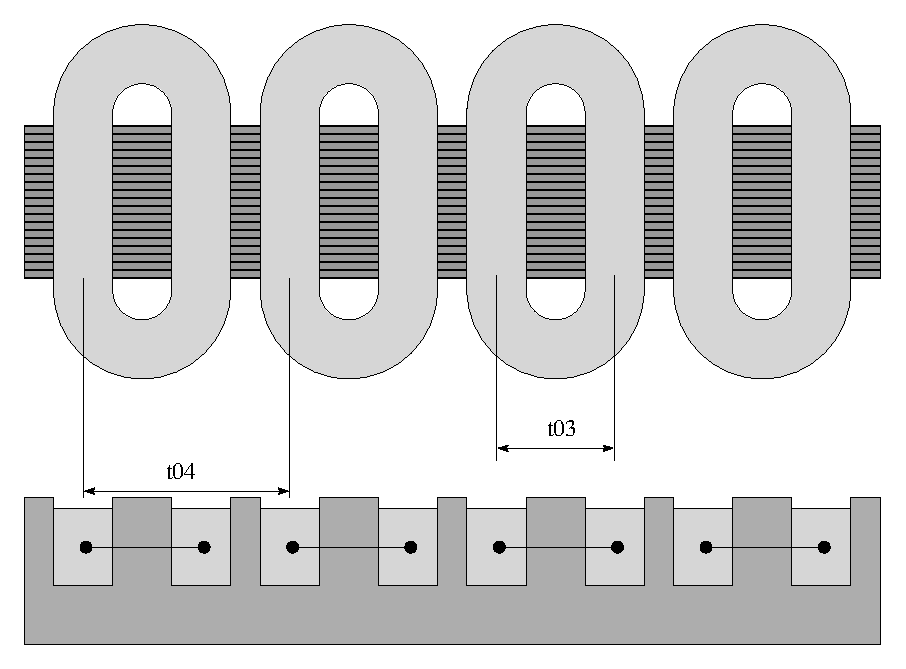
\includegraphics[width=0.42\textwidth]{figs/f_concen_coils-a.eps}
\end{psfrags}%}
  \hfill
  \subfloat[Double layer\label{fig:concen-b}]{
  \begin{psfrags}%
\psfragscanon

% text strings:
\psfrag{t01}[bc]{(a) Single layer}
\psfrag{t02}[bc]{(b) Double layer}
\psfrag{t03}[bc]{$x \tau_s$}
\psfrag{t04}[bc]{$2\tau_s$}
\psfrag{t05}[bc]{$\tau_s$}

% Figure:
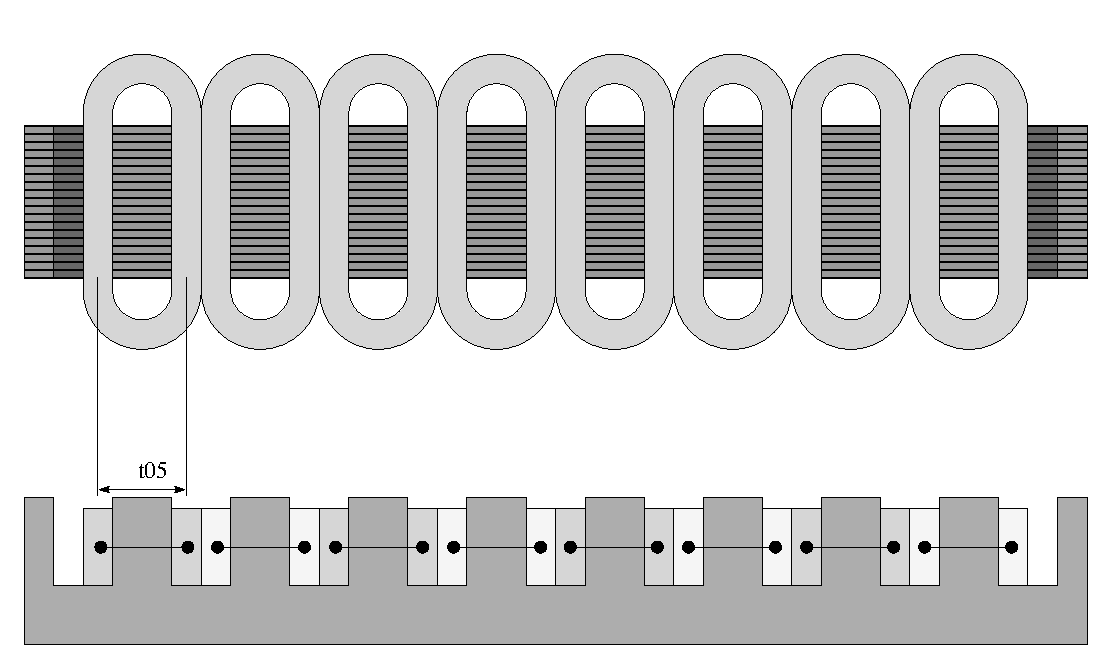
\includegraphics[width=0.52\textwidth]{figs/f_concen_coils-b.eps}
\end{psfrags}%}
  \caption{Single and double layer non-overlapping windings}
  \label{fig:concen_coils}
\end{figure}
\index{Zahnspulen}
\index{double layer}
\index{concentrated coils}
\index{tooth coils}

In the literature different definitions of terms are in use for non-overlapping concentrated windings. The most common of them are:
(a) concentrated windings \cite{REF-00822}; (b) concentrated fractional pitch windings \cite{REF-00823};  (c) fractional slot wound \cite{REF-00815}; and (d) fractional slot \cite{REF-01044}.

If the coils are to be equally in shape, which simplifies manufacturing, it is recognised that a single layer could easily have a variable slot pitch\footnote{The concept of a variable coil pitch is shown in Fig.~\ref{fig:f_slotstar}.} Furthermore, the coils could be implemented as either form-wound or round-wound. Returning to the variable coil pitch of the single layer, it is important to mention that this is an extra degree of freedom that offers to be an attractive design parameter. The air gap flux that links the coil could thus be increased and torque ripple can be improved. 
\index{regular}
\index{irregular}
\index{form-wound}
\index{round-wound}

It is therefore helpful to classify a concentrated winding either as an overlapping or non-overlapping concentrated winding. Reference \cite{REF-00754} certainly aroused interest in non-overlapping concentrated windings with their paper entitled ``Synthesis of High Performance PM Motors With Concentrated Windings'', since this is a paper which is very often used as a reference on these winding types. This could be a possible explanation for the use of the term ``concentrated windings'' rather than ``tooth coil windings''.

The expansion of the classical winding types used in machines by non-overlapping windings offers new possibilities in especially traction machine design. The main research question in section \ref{sec:problem_statement} suggests a design algorithm that takes into account the non-overlapping type. Obviously a method that is valid for all types is required. In addition, it should be easy to integrate into whichever process is in use.

\section{Notes to the reader}
The work presented in this thesis was done in N\"urnberg, Germany. Consequently many of the literature used were in German. To name only a few, books by \cite{REF-00004}, \cite{REF-00429} and \cite{REF-00294} are still commonly used in design offices. It is noticeable that even though there exists a list of symbols for various quantities, English and German have in some cases different symbols for the same quantity. This is mainly due to the fact that languages develop individual and of course colloquial language rules. Even a direct translation does not necessarily give the typical word used. An example is the German word \textit{Felderregerkurve}. A direct translation would be ``field excitation curve'', which of course is not wrong. However, the field excitation curve in electrical terms is usually known as the ``magnetomotive force'' (mmf). Tab.~\ref{tab:translation} gives some common electrical machine quantities in English and German, and the different symbols in use.
\begin{table}[htbp]
  \caption[Typical machine quantities and their German translation]%
  {Typical machine quantities, and their German counterparts}
  \label{tab:translation}
  \centering
  \begin{tabular}{lccl}
  \toprule
  Quantity   &  English  & German & Unit \\
  \toprule
  magnetomotive force (\textit{Durchflutung}) & 
  $F$& $\Theta$ & \SI{}{A}\\
  \midrule
  flux linkage (\textit{Flussverkettung}) & 
  $\lambda$& $\psi$ & \SI{}{V.s}   \\
  \midrule
  voltage (\textit{Spannung})  & 
  $V$& $U$ & \SI{}{V} \\
  \midrule
  specific resistance (\textit{spezifischer Widerstand})&
  $\rho$& $\varrho$ & \SI{}{\ohm.m} \\
  \midrule
  specific weight (\textit{spezifischer Masse})&
  $\rho$& $\gamma$& \SI{}{kg.m^{-3}}\\
  \midrule
  conductivity (\textit{Leitf\"ahigkeit})&
  $\sigma$&$\kappa$& \SI{}{S.m^{-1}}\\
  \midrule
  cross section area (\textit{Querschnitt})&
  $A$&$Q$& \SI{}{m^{2}}\\
  \midrule
  turn number (\textit{Windungszahl}) & 
  N& W & - \\
  \bottomrule
  \end{tabular}
\end{table}
\index{magnetomotive force}
\index{flux linkage}
\index{turn number}
\index{specific resistance}
\index{specific weight}
\index{Felderregerkurve}

It is commendable that the German terminology on electrical machines allows a very precise description of almost all aspects related to the subject. In many cases it is difficult to find an equivalent technical term in English, because it simply does not exist. The problem of different terminologies even exists within a language: different ``schools'' use different terms which makes the study of machine related books not easy. Also historical changes need to be kept in mind.

%The term ``machine'' is preferred throughout the book  and means it could be a machine that is operated either as a motor or as a generator. In the title the term ``motor'' is used, since only the measured results of motor operation are presented. However, in the theoretical sections, the word ``machine'' is preferred. 
%\index{machine}
%\index{motor} 

The discrete Fourier transform (DFT) has much in common with the winding factor and its definition is given in \eqref{eqn:DFTdef}. Note that the exponent is a negative number and complex. The reason for the negative exponent is explained in \cite{REF-01048,REF-01049,REF-01050}. For the complex notation a $\i$ and not a $i$ is used. Furthermore, to keep the equations compact the complex exponent will be written as $e^z$ rather than $e^{-\i\theta}$.
\begin{equation}\label{eqn:DFTdef}
  X(k)=\sum_{j=1}^{N}x(j)e^z
  \qquad
  \begin{cases}
    j \in \left\{1,\ldots,N  \right\} \rightarrow \; \mbox{sampled data}\\
  	k \in \left\{1,\ldots,N  \right\} \rightarrow \; \mbox{harmonic order}\\
    z = -\i\theta   \\
  	\theta = \frac{2\pi}{N}   \\
  	e^{-\theta \i} = \cos (-\theta) + \i \sin (-\theta)
  \end{cases}
\end{equation}
An important difference between the complex winding factor and the DFT is the phase information. In a typical DFT it is assumed that the sampled points are equidistant, i.e.~$\frac{2\pi}{N}$. The geometrical position of the stator slots around the air gap peripheral is the phase information. Through the phase information it is thus possible to calculate the winding factors for non equidistant stator slots. 

\section{Design program}
A Matlab script that implements the algorithm in Fig.~\ref{fig:flowchart} is used to plot the examples given in Tab.~\ref{tab:Example_table}. The complete program listings are given in \ref{sec:malg} and \ref{sec:mex}. Start the script by typing from the Matlab promt:

\begin{lstlisting}[language=matlab]
wnd = arun(1);
\end{lstlisting}
The resulting plots are shown in Fig.~\ref{fig:tests} and the Matlab code is provided in appendix \ref{sec:mex}.


%\chapter{A historical view of winding design}
In the first of his two remarkable papers \cite{REF-00835, REF-00836} the systematics of stator windings and the calculation of the winding factors are explained. The aim in this work was to determine the parameters that characterise the air gap mmf of the winding. Also in this paper the induced voltage in the coil sides is already mentioned and represented as a vector. The resultant vector diagram was called the star of coil groups (German: ``Spulengruppenstern''). The adjacent vectors on such a diagram that belong to the same phase is called a phase belt (German: ``Zone'').
\index{star of coil groups}
\index{Spulengruppenstern}
\index{Zone}

Two years later, in the second paper by \cite{REF-00837}, the algebraic methods developed in the first paper were visualised by means of Tingley's diagram. The latter could be referred to as a linear representation of the now called star of slots (German: ``Nutenstern''). The star of slots is constructed using the electrical angle between two adjacent slots. Computer technology as we know it today was not available at the time and the use of graph paper certainly was common. Furthermore, such graphical methods definitely contributed to the subject of stator windings.
\index{Tingley's diagram}
\index{Nutenstern}

Vil\'em Kl\'ima (Wilhelm Kauders) died on 6 October 1985 and in an obituary by \cite{REF-01054} it is mentioned that Kl\'ima's equation for the distribution factor\footnote{Also known as the breadth factor.} of fractional slot windings is not found in textbooks. Another remark in the obituary is that in some references it is stated that it is not possible to find a closed-form expression for the winding factor of fractional slot windings. In the rest of this literature overview, none of the authors (except Kremser) refers to or makes use of Kl\'ima's closed-form expression. 

More than fifty years later \cite{REF-00837}, \cite{REF-00266} introduced a comprehensive study of fractional slot windings and the currents in the parallel paths of rotating machines. The reason for this big time gap does not mean that nothing had happened in the mean time in winding design; it should be kept in mind that this overview only points out some important aspects. In the first part of Kremser's doctoral thesis a detailed algebraic description of single and double layer fractional slot windings is presented. In order to allocate the coils to the stator slots, modular arithmetic, which uses the so-called commutator pitch, is used. This can be seen as a step toward using computer programs to automatically performing winding designs. In the star of slots the vectors start wrapping, and once put on a graph, two vectors having angles of \ang{45} and \ang{405} respectively lie exactly on each other. The star of slots is thus the same as the remainder after dividing an angle by \ang{360} which can easily be implemented by means of the modulo function.  
\index{modular arithmetic} 
\index{commutator pitch}  

The author in \cite{REF-00452} explains another algebraic method to design stator windings which has much in common with that presented by \cite{REF-00266}\footnote{It should however be noticed that the authors Wach and Kremser are from Poland and Germany respectively.}.  The methods presented in the paper is characterised by the matrix representation of a winding. The winding matrix simplify the winding factor calculation and avoids complex equations. Basically the vectors of the star of slots is used in matrix form. What is called the winding matrix could be seen as the matrix representation of Tingley's diagram. A drawback of the method is that each matrix entry for double layer windings has two values. In computer programming this should be solved by either a multi-dimensional matrix or two two-dimensional matrices. In another paper by \cite{REF-00454}, the focus is on the optimisation of fractional slot windings. In spite of the fact that this paper is a very good source on the topic of winding design, none of the literature in the rest of this section refers to it.
 
The use of stator coils wound around the stator teeth has some attractive advantages for manufacturing as shown \cite{REF-00754}. The coils do not overlap which means that the manufacturing is simplified and the winding overhang is less than that of overlapping windings. Electrically the shorter winding overhang means the use of less copper. Furthermore, the non-overlapping windings are derived from single or double layer overlapping windings. It is also pointed out that in the case of single layer non-overlapping windings the coil pitch can be increased and used as a design parameter\footnote{See Fig.~\ref{fig:f_slotstar} for regular and irregular distributed slots.}. The latter, however, is not taken into account in the winding factor calculation. This paper is referenced quite often, proving the interest among machine designers in non-overlapping windings.  

An extensive study on fractional slot windings for low speed applications is presented in \cite{REF-01055}. The main objective in the doctoral thesis is to compare different slot combinations of a machine with a fixed air gap diameter in the \SI{45}{kW} range. Although both single and double non-overlapping windings are taken into account, the focus is on the double layer type. Since round wire coils are used in the investigated application it is appropriate to use a double layer rather than single layer. If form-wound coils were used the choice of double layer windings would have caused some difficulties when inserting the coils into the stator slots. Also, the stator had semi-closed slots. The star of slots is referred to as the voltage vector graph in Salminen's thesis. A very important comment by the author is that care should be taken when the winding factors for different winding types are to be calculated. Depending on the winding type the right set of equations should be chosen. 

The proposed a method in \cite{REF-00756} to calculate the winding factors for concentrated coils does not require any knowledge of the winding layout. This is of course sufficient to quickly compare different slot and pole combinations. Using this method it is shown that the best number of slots per pole and phase should be in the range \textonequarter $\leq q\leq$ \textonehalf. 

The tutorial presented by \cite{REF-01056} is an in-depth study of fractional slot windings in general. In their tutorial notes a distinction is made between overlapping and non-overlapping windings. Here too the non-overlapping type is derived from a double layer overlapping winding. 
%\chapter{Classification of symmetrical windings}
This report\footnote{Text taken from \cite{REF-00014}.} is devoted to a derivation of an algorithmic method to design $m$-phase symmetrical windings and a representation thereof in a compact form. The basic principle of the winding of an electrical machine is to obtain a rotating magnetic field in the stator (the stationary part) that interacts with the moving part (the rotor). This is achieved by arranging the coils of the winding in the stator slots around the air gap periphery in such a way that a rotating field is developed when applying currents. As a result the induced voltage, which arises from flux per pole $\hat{\Phi}$, is obtained from Faraday's law. In general the sinusoidally induced voltage for a winding having $N_s$ series turns per phase is
\begin{equation}
  \label{eqn:ui}
  U_i = \sqrt{2} \pi f_1 \xi_p N_s \hat{\Phi}, \qquad \xi_p \leq 1
\end{equation}
where $\xi_p$ is the winding factor of the \textit{working harmonic}. The induced voltage in \eqref{eqn:ui} brings the importance of the winding design to the fore. For a given design requirement, it is desirable to have $\xi_p$ as high as possible.

\section{Definition of the working harmonic}\label{sec:working_harmonic}
Throughout the analysis all harmonics are referred to in terms of the bore $2\pi$ of the machine, i.e.~the \textit{fundamental harmonic} has the order $\nu=1$ and forms one pole pair. The harmonic that produces the magnetic field that interacts with the rotor poles $2p$ has the order $\nu=p$ and is called the \textit{working harmonic}. Any other harmonic of the $\nu^{th}$ order will have $\nu$ pole pairs and spans a peripheral angle of $\frac{2\pi}{\nu}$.
\index{working harmonic}

Often the harmonic orders are normalised with respect to the \textit{working harmonic}, i.e.~$\xi_{\nu /p}$. This then means that the \textit{working harmonic} is written as $\xi_1$ and sub-harmonics will have a fraction as subscript. This notation will not be used in this report.

\section{Basic winding properties}%
\label{sec:m_phases}
The winding design can be quite a difficult task and at this point it is useful to have a coarse classification of symmetrical windings. Since symmetrical windings comprise such a great variety, an attempt to categorise them will depend on the properties by which they are to be sorted. 

\subsection{Slots and coils per pole and phase} \label{subsec:slots_coils}
Any $m$-phase winding could be characterised by its number of slots per pole and phase. However, when comparing different winding designs with each other this number alone is insufficient. It does not take into account the number of layers the winding has. In addition, the number of coils per pole and phase should be defined. For a machine with $Q_s$ stator slots, $p$ pole pairs and $m$ phases the following definitions holds:

\begin{defth}
Slots per pole and phase: 
\begin{equation}
  q =\frac{Q_{s}}{m2p}=\frac{q_{n}}{q_{d}}
\end{equation}
$\frac{q_{n}}{q_{d}}$ is the reduced form of $q$. Each phase has $q_n$ slots that are distributed over $q_d$ poles. In the case where $q_d$ equals one, $q$ is an integer and the winding is called an integer slot winding. When $q_d$ is greater than one, it is called a fractional slot winding. 
\end{defth}
\begin{defth}
Coils per pole and phase: 
\begin{equation}
  q_{c}=\frac{Q_{c}}{m2p}=\frac{q_{c_n}}{q_{c_d}}
\end{equation}
$\frac{q_{c_n}}{q_{c_d}}$ is the reduced form of $q_c$. Each phase has $q_{c_n}$ coils distributed over $q_{c_d}$ poles. If $q_{c_n}$ is greater than one and $q_c$ is not equal to one it is a distributed winding. 
\end{defth}
These characteristic numbers give useful information on the winding when they are written as a reduced improper fraction\footnote{The reduced fraction could be either a proper or an improper fraction. An improper fraction has the numerator greater than the denominator.}. Additionally, the properties of single and double layer windings are summerised in Tab.~\ref{tab:properties_single_double}. 
\index{slots per pole and phase}
\index{reduced form}
\index{coils per pole and phase}

{\renewcommand{\arraystretch}{1.2}
\begin{table}[htbp]
  \caption{Winding properties}
  \label{tab:properties_single_double}
  \centering
  \begin{tabular}{|c|c|}
  \hline
  single layer winding & double layer winding \\
  \hline
  $q = 2q_c$ & $q = q_c$ \\
  $Q_s = 2Q_c$ &  $Q_s = Q_c$ \\
  \hline
  \end{tabular}
\end{table}}
\index{winding properties}

\subsection{Average coil pitch}
The coil pitch is defined as the peripheral angle between the two coil sides. It is practical to express the coil pitch in terms of the number of slots. Therefore, it is an integer number. 
\begin{defth}
The average coil pitch is defined as
\begin{equation}
  \label{eqn:y_p}
  y_p = \frac{Q_s}{2p}
\end{equation}
and the implemented coil pitch is given by
\begin{equation}
  \label{eqn:y_d}
  y_d = \mbox{int}(y_p)\pm k
  \quad
  \begin{cases}
    k \in \mathbb{N} \\
    y_d \geq 1
  \end{cases}
\end{equation}
\end{defth}
In the case where $y_d=y_p$ it is a full-pitch winding. If $y_d \neq y_p$ it is called a fractional pitch winding. 
\index{average coil pitch}

\subsection{Classification scheme}
The aim of the classification scheme is to find a way to relate different winding types to each other. It is also a useful guideline to compare windings that belong to the same category. For the design methodology offered in this report, the following winding parameters are chosen for the classification:
\begin{enumerate}
  \item the reduced form of the number of coils per pole per phase;
  \item the average coil pitch; and 
  \item the number of layers.
\end{enumerate}
Tab.~\ref{fig:classification} shows a possible way to classify symmetrical $m$-phase windings. The reason for choosing the average coil pitch as a second property arises from the construction of the coils and it is valid for all types of windings. It could be seen as the ideal coil pitch. Additionally, the number of layers is a key parameter since the technology for manufacturing and the material used in single layer windings are different from that used in double layer windings. Using this classification scheme, the following definitions are associated with windings:
\begin{description}
  \item[Distributed winding:] If the numerator $q_{cn}$ of $q_c$ is greater than~%
  one, the winding is distributed. This means that the coil sides are distributed~%
  over $q_{cn}$ slots. The opposite of a distributed winding is a concentrated~%
  winding.
  \item[Concentrated winding:] In the case where $q_{c_n}$ equals one, it is called~%
  a concentrated winding. 
  \item[Concentrated coil:] When $y_d$ equals one, it is a concentrated coil. In~%
  this case the coil is concentrated around a stator tooth.
  a concentrated winding. 
  \item[Single and double layer:] These windings are differentiated by the number~%
  of coils compared to the number of stator slots. In single layer windings the~%
  number of coils equals half the number of stator slots, while for double layer~%
  windings the number of coils is equal to the number of stator slots. In the~%
  present dissertation a double layer winding has two coil sides per slot which could~%
  placed radially in two layers or side by side. 
  \item[Overlapping and non-overlapping:] In overlapping windings the coils overlap~%
  and the coil pitch $y_d$ is greater than one. If the coil pitch $y_d$ equals one,~%
  the coils do not overlap.
  \item[Integral slot winding:] If the denominator $q_d$ equals one, the phase~%
  belt has $q_n$ slots over one pole.
  \item[Fractional slot:] The denominator of $q$ is greater than one. This~%
  means that the $q_n$ slots are distributed over $q_d$ poles. In addition,~%
  the average coil pitch $y_p$ is a fraction. 
\end{description}
{\renewcommand{\arraystretch}{1.2}
\begin{table}[htbp]
  \centering
  \caption{Classification of symmetrical windings}
  \label{fig:classification}
  \begin{tabular}{|l|l|l|}
  \hline
  Parameter  & Constraint  &  Classification  \\
  \hline
  \multirow{2}{*}{$Q_c$} & $\frac{1}{2}Q_s$ & single layer \\
                         & $Q_s$            & double layer \\
  \hline                        
  \multirow{2}{*}{$y_d$} & $=1$  & non-overlapping         \\
                         & $>1$  & overlapping             \\
  \hline                         
  \multirow{2}{*}{$y_d$} & $=y_p$     & full-pitch         \\
                         & $\neq y_p$ & fractional pitch   \\
  \hline                         
  \multirow{2}{*}{$q_d$} & $=1$     & integral slot        \\
                         & $>1$     & fractional slot      \\
  \hline                         
  \multirow{2}{*}{$q_{c_n}$} & $=1$     & concentrated     \\
                             & $>1$     & distributed      \\  
  \hline
  \end{tabular}
\end{table}}

It is important to distinguish between a concentrated winding and a concentrated coil. The classification scheme in Fig.~\ref{fig:classification} defines a concentrated winding in a unique way. Concentrated windings are defined differently in literature. \cite{REF-00814} refers to it as a traditional single layer winding whereas \cite{REF-00822} refers to it as distributed.
\index{concentrated winding}
\index{concentrated coil}
\index{classification scheme}
\index{distributed winding}

Particularly the windings defined as a fractional slot are very attractive for use in permanent magnet synchronous machines. Especially the single layer non-overlapping winding could be used to reduce (a) manufacturing costs compared to overlapping windings; (b) the end winding losses; (c) torque ripple; and (d) the mutual coupling between the phases.
\index{manufacturing costs}
\index{end winding losses}
\index{torque ripple}
\index{mutual coupling}

\section{Characteristics of symmetrical windings}
This section contains the major properties by which symmetrical $m$-phase windings are characterised.

\subsection{Basic winding}
\begin{defth}
The smallest repetitive segment is called the basic winding (German: ``Urwicklung'').
\end{defth} 
Due to symmetry only the basic winding needs to be determined. If $q_d$ is less than $p$ the winding is composed of $t$ identical \textit{basic windings}, i.e.
\begin{equation}
  \label{eqn:gcd_t}
  \begin{array}{ll}
  t = \begin{cases}
        \gcd\left(Q_s,p\right)  & \text{for double layer}\\
        \gcd\left(\frac{Q_s}{2},p\right) & \text{for single layer}
      \end{cases}
  \end{array}
\end{equation}
and gcd is called the greatest common divisor. In the case where $t=1$ the winding has no symmetry. Each of the $t$ \textit{basic windings} will have $Q_b$ slots and $p_b$ pole pairs, therefore
\begin{equation}
  \label{eqn:qd_pb}
  Q_b = \frac{Q_s}{t} \quad \mbox{and} \quad p_b = \frac{p}{t} 
\end{equation}
The number $p_b$ is the reduced pole pair. Another way of obtaining this number is by means of the denominator of $q_c$, i.e.
\begin{equation}
  \label{eqn:p_b}
  p_b =  
  \begin{cases}
    \frac{1}{2} q_{c_d}  & q_{c_d} \: \textnormal{even} \\
    q_{c_d}  & q_{c_d} \: \textnormal{odd}
  \end{cases}
\end{equation} 
which is independent of $t$. Examining \eqref{eqn:gcd_t}, it is recognised that $t$ can be rewritten as the gcd between the number of coils and the pole pairs, i.e.
\begin{equation}
  \label{eqn:gcd_t_gcd(Qc_p)}
  t = \gcd(Q_c,p) \quad
  \begin{cases}
    Q_c = Q_s \quad & \textnormal{double layer} \\
    Q_c = \frac{1}{2}Q_s \quad & \textnormal{single layer}
  \end{cases}
\end{equation} 
which is valid for both single and double layer windings. Although $t$ is usually used as a variable for time it is commonly found in literature and will be used in the same way throughout this chapter. Since the winding design is independent of time, it does not cause any confusion.

It is favourable to use the terms ``in and out going coil sides''\footnote{This is similar to the current which is defined as into and out of the page.}. Only the in going coil side needs to be assigned\footnote{The use of coil sides are preferred above coils, since it is then independent whether the coil sides belong to the same coil or not.} since the out going coil side is given by the coil pitch and type of winding.

\subsection{Winding symmetry}
For a winding to be symmetrical the number of coils used in each of the phases must be equal. Therefore the quotient between $Q_c$ and $m$ must be an integer. A requirement for a winding to be symmetrical can be derived from \eqref{eqn:qd_pb}. The symmetry condition can be expressed as
\begin{equation}
  \label{eqn:feasibility}
  \frac{Q_s}{t} = mk, \quad  k \in  \mathbb{N}
\end{equation}
which relates the pole number, number of stator slots and phase number to each other. A very useful function employed in the method is the modulo function which finds the remainder after division, i.e.~ $\textnormal{mod}(a,b)=a-\textnormal{floor}(\frac{a}{b})$\footnote{The floor function of a real number $x$, floor($x$), is a function whose value is the largest integer less than or equal to $x$.}. When using the modulo function it means that $\textnormal{mod}(\frac{Q_s}{t},m)$ must equal zero. There are different ways of deriving the constraints for the winding symmetry condition. Tab.~\ref{tab:feasibility} gives different variations found in the literature to express the symmetry condition. 
{\renewcommand{\arraystretch}{1.6}
\begin{table}[h]
  \caption{Constraints for symmetry}
  \label{tab:feasibility}
  \centering
  \begin{tabular}{|l|l|}
  \hline
  Reference & Constraint \\
  \hline
  \multirow{2}*{\cite{REF-00452}} & $\gcd(q_{c_d},m)=1$  \\
  &$\mbox{mod}\bigl(\frac{Q_c}{q_{c_n}}q_{c_d},m\bigr)=0$\\
  \hline
  \cite{REF-00754} & $\mbox{mod}\bigl(\frac{Q_s}{\gcd(Q_s,2p)},m\bigr)=0$  \\
  \hline
  \cite{REF-00486} & $\mbox{mod}\bigl(\frac{Q_s}{t},m\bigr)=0$ \\
  \hline
  \end{tabular}
\end{table}}

\subsection{Reduced number of pole pairs}
The lowest harmonic generated by a winding is given by $t=\gcd\left(Q_c,p\right)$ and the working harmonic equals $p$. The reduced pole number gives information on the sub-harmonics which are summarised as follows:
\begin{equation}  
 \begin{aligned}
  t &= p \quad \textnormal{the winding has no sub-harmonics} \\
  t &< p \quad \textnormal{the winding has sub-harmonics}
  \end{aligned}
\end{equation} 

The reduced number of pole pairs can be calculated in two different ways. Two greatest common divisors, i.e.~$\gcd\left(Q_c,2\,m\,p\right)$ and $\gcd\left(Q_c,p\right)$, are used to get $q_{c_d}$ and $p_b$ respectively. The relationship between these two factors is as follows:
\begin{equation}
  \label{eqn:reduced_p} 
  \gcd\left(Q_c,p\right)=\frac{\gcd\left(Q_c,2\,m\,p\right)}{r} \hspace{15pt}
  \textnormal{where} \hspace{15pt} r=
  \begin{cases}
   m  & \text{$q_{c_d}$ even}\\
   2m & \text{$q_{c_d}$ odd}
  \end{cases}
\end{equation}

\section{Rotating mmf}
Distributing the coils around the air gap periphery firstly requires the winding characteristic as explained in section \ref{subsec:slots_coils} and secondly a constraint assuring that the coils are assigned uniquely to the stator slots. Deriving such a constraint is done by means of the magnetomotive force (mmf) produced by a winding. 
\index{magnetomotive force}

In the theory of three-phase windings the rotating magnetic field is derived from a single coil with $N_t$-turns. The mmf produced by the coil is then written as a Fourier series which allows it to be decomposed in the \textit{working harmonic}, higher order harmonics and sub-harmonics if applicable. A detailed mathematical derivation is given by \cite{REF-01043}. It is also possible to explain the decomposition by means of visualisation as shown in \cite{REF-00004}, \cite{REF-00294} and  \cite{REF-00330}. The visualisation method is preferred and is used in the next sections in order to define the mmf envelope functions. This is necessary to answer the research sub-question which is the mathematical expression that defines a phase belt.
\index{harmonics}
\index{sub-harmonics}

\subsection{The mmf of a single turn coil}%
\label{subsec:nt-turn_coil}
Consider a single coil with $N_t$-turns carrying a current $i$ placed in the stator of a machine with a uniform air gap as shown in Fig.~\ref{fig:mmf_1}\subref{fig:sincol}. Assuming an infinite permeability in the laminated parts, the mmf in the stator and rotor can be neglected. This means the mmf across the air gap will be equal to the total mmf. 
 
\begin{figure}[htbp]
  \centering
  \fontsize{8}{10}\selectfont
  \subfloat[Single coil\label{fig:sincol}]{
  \begin{psfrags}%
\psfragscanon

% text strings:
\psfrag{x01}{$0$}
\psfrag{x02}{$\frac{\pi}{3}$}
\psfrag{x03}{$\frac{2\pi}{3}$}
\psfrag{x04}{$\pi$}
\psfrag{x05}{$\frac{4\pi}{3}$}
\psfrag{x06}{$\frac{5\pi}{3}$}
\psfrag{x07}{$2\pi$}

\psfrag{t01}{-1}
\psfrag{t02}{+1}
\psfrag{t03}{$C_2$}
\psfrag{t04}{$C_1$}
\psfrag{t05}{$F$}
\psfrag{t06}{$\frac{4}{\pi}\frac{N_ti}{2}\sum\limits_{\nu=1}^{\infty}
            \frac{1-(-1)^{\nu}}{2} \frac{1}{\nu}\cos(\nu \theta)$}
\psfrag{t07}[br]{$\theta$}
\psfrag{t08}{$\mu \rightarrow \infty$}
\psfrag{t09}{magnetic}
\psfrag{t10}{axis}
\psfrag{t11}{$p_1$}
\psfrag{t12}{$\theta^{+}$}
\psfrag{t13}{$\frac{4}{\pi}\frac{N_ti}{2}\cos \theta$}
\psfrag{t14}{current sheet}
\psfrag{t15}{$N_t i$}
\psfrag{t16}{$C_3$}
\psfrag{t17}{(a)}
\psfrag{t18}{(b)}
\psfrag{t19}{$\delta$}

% Figure:
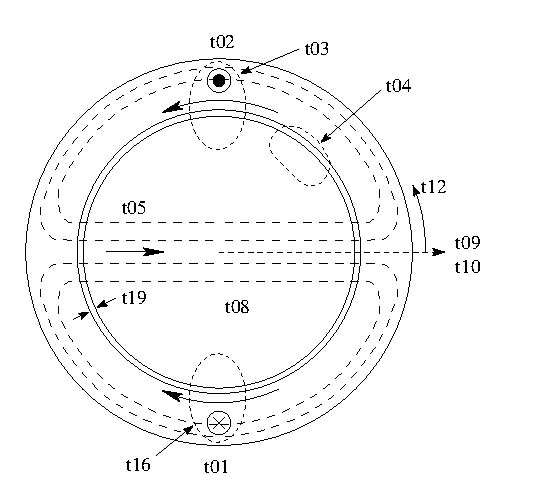
\includegraphics[height=5.5cm]{figs/f_mmf_1a.eps}
\end{psfrags}%}
  \hfill
  \subfloat[Spatial mmf distribution\label{fig:spatmmf}]{
  \begin{psfrags}%
\psfragscanon

% text strings:
\psfrag{x01}{$0$}
\psfrag{x02}{$\frac{\pi}{3}$}
\psfrag{x03}{$\frac{2\pi}{3}$}
\psfrag{x04}{$\pi$}
\psfrag{x05}{$\frac{4\pi}{3}$}
\psfrag{x06}{$\frac{5\pi}{3}$}
\psfrag{x07}{$2\pi$}

\psfrag{t01}{-1}
\psfrag{t02}{+1}
\psfrag{t03}{$C_2$}
\psfrag{t04}{$C_1$}
\psfrag{t05}{$F$}
\psfrag{t06}{$\frac{4}{\pi}\frac{N_ti}{2}\sum\limits_{\nu=1}^{\infty}
            \frac{1-(-1)^{\nu}}{2} \frac{1}{\nu}\cos(\nu \theta)$}
\psfrag{t07}[br]{$\theta$}
\psfrag{t08}{$\mu \rightarrow \infty$}
\psfrag{t09}{magnetic}
\psfrag{t10}{axis}
\psfrag{t11}{$p_1$}
\psfrag{t12}{$\theta^{+}$}
\psfrag{t13}{$\frac{4}{\pi}\frac{N_ti}{2}\cos \theta$}
\psfrag{t14}{current sheet}
\psfrag{t15}{$N_t i$}
\psfrag{t16}{$C_3$}
\psfrag{t17}{(a)}
\psfrag{t18}{(b)}
\psfrag{t19}{$\delta$}

% Figure:
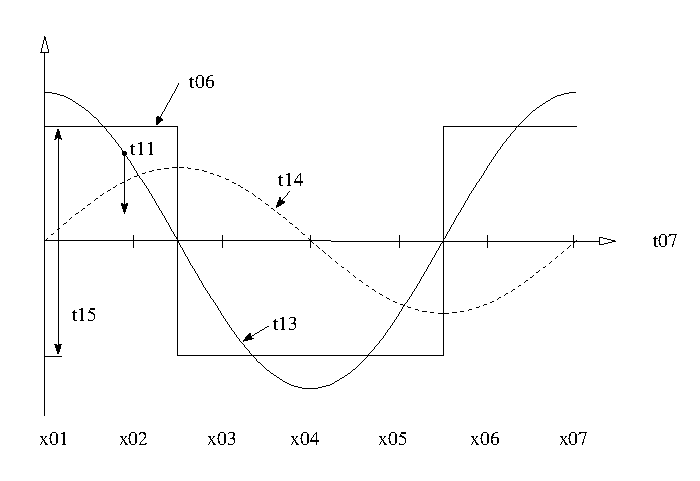
\includegraphics[height=5.5cm]{figs/f_mmf_1b.eps}
\end{psfrags}%}
  \caption{Single $N_t$-turn coil}
  \label{fig:mmf_1}
\end{figure}

The spatial mmf distribution around the air gap periphery is obtained by applying Amp\`ere's law to the contours $C_1$, $C_2$ and $C_3$. The results of the integration are given in \eqref{eqn:int_H}. The integral along $C_1$ is zero since the contour does not enclose any source. Contrary to this the integrals along $C_2$ and $C_3$ equal $N_ti$ and $-N_ti$ respectively. The current in coil side $+1$ is positive, and using the right hand rule, out of the page.  
\begin{equation}
 \label{eqn:int_H}
 \oint \vec{H} \cdot d\vec{l}=
 \begin{cases}
   \begin{array}{llll}
     0  & C_1 & 0 \leq \theta < \frac{\pi}{2} 
     & \Rightarrow H(0)=H(\theta_1)\\
     N_ti & C_2 & \frac{\pi}{2} \leq \theta < \frac{3\pi}{2} 
     & \Rightarrow H(0)-H(\theta_2) = \frac{N_ti}{\delta} \\
     -N_ti & C_3 & \frac{3\pi}{2} \leq \theta < \frac{5\pi}{3} 
     & \Rightarrow H(0)-H(\theta_3) = \frac{N_ti}{\delta}
   \end{array}
 \end{cases}
\end{equation}
Since the flux to and from the rotor are equal, the air gap mmf will have an amplitude of $\frac{N_ti}{2}$. Fig.~\ref{fig:mmf_1}\subref{fig:spatmmf} shows the spatial of the single coil. This is a square wave and from the Fourier series the fundamental has an amplitude of $\frac{4}{\pi}$. The fundamental mmf can be seen as the result of a sinusoidally distributed current sheet on the stator inner diameter. When the coil is supplied by a current 
\begin{equation}
  i = \hat{I}\cos\omega t
\end{equation}
any point on the mmf will have a vertical trajectory. For example, the point $p_1$ will start moving downward for $t^+$ until it reaches a minimum from where it will start to move upwards again. Applying a sinusoidal current to the coil results in a standing wave in the air gap. The spatial mmf distribution has the form
\begin{equation}
  \label{eqn:F_theta_t_1}
  F(\theta,t) = \frac{4}{\pi}\frac{N_t }{2}\cos\theta \left(\hat{I}\cos \omega t\right)
\end{equation}
and will have nodes at $\frac{\pi}{2}$ and $\frac{3\pi}{2}$ while the anti-nodes will be at $0$ and $\pi$. Using a trigonometrical identity\footnote{$\cos A \cos B = \frac{1}{2}\cos(A-B)+\frac{1}{2}\cos(A+B)$} \eqref{eqn:F_theta_t_1} can be rewritten as the superposition of two rotating waves
\begin{equation}
  \label{eqn:F_theta_t_2}
  \begin{aligned}
  F(\theta,t) &= \frac{1}{2}\frac{4}{\pi}\frac{N_t }{2}\hat{I}\cos(\theta - \omega t)
  +\frac{1}{2}\frac{4}{\pi}\frac{N_t }{2}\hat{I}\cos(\theta + \omega t) \\
  &= F^+ + F^-
  \end{aligned}
\end{equation}
The result in \eqref{eqn:F_theta_t_2} means that a single coil produces two opposite rotating mmf waves in the air gap. In the next section this result is used to produce a single rotating mmf by displacing different coils in space. 

\subsection{The mmf of three single turn coils}
Producing a single rotating mmf wave using three coils means that each of the spatial mmf distribution functions must have a displacement for both the spatial and time component. Using \eqref{eqn:F_theta_t_2}, the resultant mmf for three coils will have the following form, i.e.
\begin{equation}
  \begin{aligned}
  F_R(\theta,t) &= (F_{1}^{+}+F_{1}^{-})+(F_{2}^{+}+F_{2}^{-})+(F_{3}^{+}+F_{3}^{-})\\
  &=(F_{1}^{+}+F_{2}^{+}+F_{3}^{+})+(F_{1}^{-}+F_{2}^{-}+F_{3}^{-})\\
  &=\sum_{n=1}^{3}F_{n}^{+}+\sum_{n=1}^{3}F_{n}^{-}
  \end{aligned}
\end{equation}
In general, choosing an angle of $\frac{2\pi}{m}$ between two adjacent positive coil sides will cause the negative waves to be cancelled. Thus, the positive waves are added together; this results in a single rotating wave. For $m$-phases the functions defined by
\begin{equation}
  \label{eqn:F_theta_t_3}
  F_n(\theta,t)=\hat{F_n}\cos\left[\theta+\frac{2\pi(n-1)}{m}\right]
  \cos\left[\omega t +\frac{2\pi(n-1)}{m}\right], \quad 1 \leq n \leq m
\end{equation}  
will produce a rotating wave when supplied by three-phase currents that is phase shifted by $\frac{2\pi}{m}$ radians. Setting $m=1$ in \eqref{eqn:F_theta_t_3} will be the same as \eqref{eqn:F_theta_t_1}. The summation of $m$ functions given in \eqref{eqn:F_theta_t_3} simplifies to a single rotating mmf in the air gap. Using the trigonometric identity the resultant air gap mmf is
\begin{equation}
  \label{eqn:F_theta_t_4}
  \begin{aligned}
  F_R(\theta,t)&=\sum_{n=1}^{m}\hat{F_n}\cos\left[\theta+\frac{2\pi(n-1)}{m}\right]
  \cos\left[\omega t +\frac{2\pi(n-1)}{m}\right] \\
  &=\frac{1}{2}\sum_{n=1}^{m}\hat{F_n}\cos(\theta-\omega t)+
  \frac{1}{2}\sum_{n=1}^{m}\hat{F_n}
  \cos\left[\theta+\omega t+\frac{4\pi(n-1)}{m}\right] \\
  &=\frac{m}{2}\hat{F_1}\cos(\theta-\omega t)
  \end{aligned}
\end{equation} 
Therefore, the effect of displacing the positive coil sides of $m$-coils by $\frac{2\pi}{m}$ radians results in a single rotating mmf wave in the air gap which is $\frac{m}{2}$ times that of the first coil.

The preceding explanation of the rotating mmf wave is graphically shown in Fig.~\ref{fig:mmf_2}(a). Therefore, starting with a single coil as in Fig.~\ref{fig:mmf_1}(a) means it is necessary to add two more coils. Using the positive coil side of $+1$ as reference, the adjacent positive coil side $+2$ is placed at $-\frac{2\pi}{3}$ radians clockwise from \num{+1}. Next, with \num{+2} as reference the next adjacent positive coil side is $-\frac{2\pi}{3}$ radians clockwise from $+2$. The returning coil sides of both coils is displaced at $+\pi$ electrical radians in space. Since the resultant mmf wave is rotating in a positive direction the sequence\footnote{The direction of placing the positive coil sides and the returning coil sides is arbitrary. When the convention as explained is used, it simplifies the code which automatically does the coil assignment.} will be 
\begin{equation}
  \label{eqn:phasebelt_sequence}
  \{+1,\ -2,\ +3,\ -1,\ +2,\  -3\} 
\end{equation}

\begin{figure}
  \centering
  \fontsize{8}{10}\selectfont
  \subfloat[Three coils\label{fig:threecoils}]{
  \begin{psfrags}%
\psfragscanon

% text strings:
\psfrag{x01}{$0$}
\psfrag{x02}{$\frac{\pi}{3}$}
\psfrag{x03}{$\frac{2\pi}{3}$}
\psfrag{x04}{$\pi$}
\psfrag{x05}{$\frac{4\pi}{3}$}
\psfrag{x06}{$\frac{5\pi}{3}$}
\psfrag{x07}{$2\pi$}

\psfrag{c01}[bc]{+1}
\psfrag{c02}{-2}
\psfrag{c03}{+3}
\psfrag{c04}[bc]{-1}
\psfrag{c05}{+2}
\psfrag{c06}{-3}
\psfrag{t03}{$\mu \rightarrow \infty$}
\psfrag{t05}{$F$}
\psfrag{t07}[br]{$\theta$}
\psfrag{t08}{$F_2$ envelope}
\psfrag{t09}{magnetic}
\psfrag{t10}{axis}
\psfrag{t11}{$F_1$}
\psfrag{t12}{$F_2$}
\psfrag{t13}{$F_3$}
\psfrag{t14}{phase belt}
\psfrag{t15}{$-\frac{2\pi}{3}$}
\psfrag{t16}{$-\frac{2\pi}{3}$}
\psfrag{t17}{$+\pi$}
\psfrag{t18}{$\theta^{+}$}

\psfrag{t19}{(a)}
\psfrag{t20}{(b)}

\psfrag{p01}{$p_1$}
\psfrag{p02}{$p_2$}
\psfrag{p03}{$p_3$}
\psfrag{p04}{$p_4$}

% Figure:
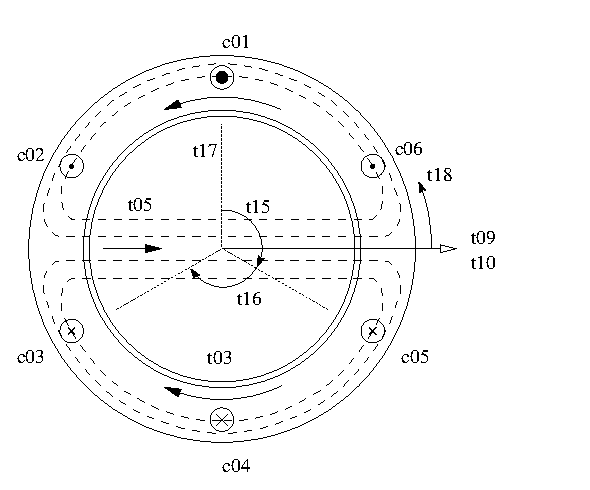
\includegraphics[height=5.3cm]{figs/f_mmf_2a.eps}
\end{psfrags}%}
  \hfill
  \subfloat[Spatial mmf distribution\label{fig:nt3mmf}]{
  \begin{psfrags}%
\psfragscanon

% text strings:
\psfrag{x01}{$0$}
\psfrag{x02}{$\frac{\pi}{3}$}
\psfrag{x03}{$\frac{2\pi}{3}$}
\psfrag{x04}{$\pi$}
\psfrag{x05}{$\frac{4\pi}{3}$}
\psfrag{x06}{$\frac{5\pi}{3}$}
\psfrag{x07}{$2\pi$}

\psfrag{c01}[bc]{+1}
\psfrag{c02}{-2}
\psfrag{c03}{+3}
\psfrag{c04}[bc]{-1}
\psfrag{c05}{+2}
\psfrag{c06}{-3}
\psfrag{t03}{$\mu \rightarrow \infty$}
\psfrag{t05}{$F$}
\psfrag{t07}[br]{$\theta$}
\psfrag{t08}{$F_2$ envelope}
\psfrag{t09}{magnetic}
\psfrag{t10}{axis}
\psfrag{t11}{$F_1$}
\psfrag{t12}{$F_2$}
\psfrag{t13}{$F_3$}
\psfrag{t14}{phase belt}
\psfrag{t15}{$-\frac{2\pi}{3}$}
\psfrag{t16}{$-\frac{2\pi}{3}$}
\psfrag{t17}{$+\pi$}
\psfrag{t18}{$\theta^{+}$}

\psfrag{t19}{(a)}
\psfrag{t20}{(b)}

\psfrag{p01}{$p_1$}
\psfrag{p02}{$p_2$}
\psfrag{p03}{$p_3$}
\psfrag{p04}{$p_4$}

% Figure:
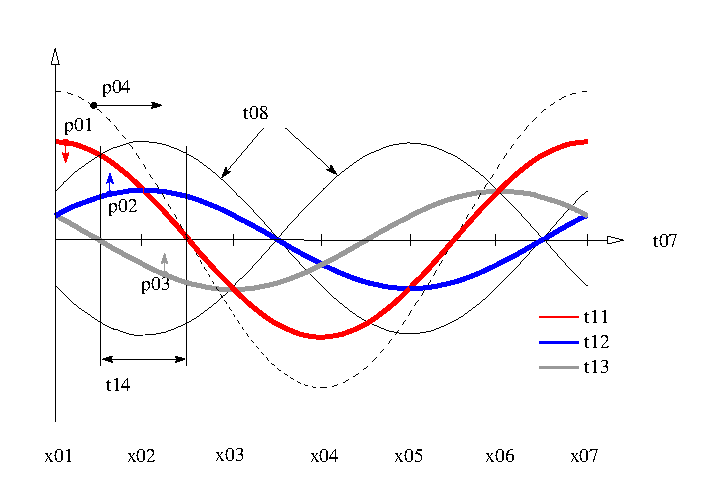
\includegraphics[height=5.3cm]{figs/f_mmf_2b.eps}
\end{psfrags}%}
  \caption{Three $N_t$-turn coils}
  \label{fig:mmf_2}
\end{figure}

Fig.~\ref{fig:mmf_2}\subref{fig:threecoils} shows graphically the mmf's of the three coils with $N_t$-turns. These are obtained by setting $m=3$ and applying the following three-phase currents 
\begin{equation}
  \label{eqn:3ph_i}
   i_n = \hat{I}\cos\left(\omega t +(n-1)\frac{2\pi}{m}\right),
  \qquad
  1 \leq n \leq m
\end{equation}
to the functions in \eqref{eqn:F_theta_t_3}. The resultant mmf will rotate in a counterclockwise direction. At $t=0$ $i_2=i_3=-\frac{1}{2}i_1$, meaning the mmf of $F_2$ and $F_3$ will be half of $F_1$. As time starts to increase, any point on $F_1$ will move downward while points on $F_2$ and $F_3$ will start moving in an upward direction. The points are marked $p_1$ through $p_3$ in the figure. Contrary to this, any point on the resultant mmf will start moving in the right direction (counter-clockwise) as indicated by point $p_4$. As time increases the resultant mmf rotates as shown in Fig.~\ref{fig:rotating_wave}. The fundamental mmf is shown at time equal to zero and a time instant $t=t_1$.
\begin{figure}
  \centering
  \fontsize{8}{0}\selectfont
  \subfloat[$t=0$\label{fig:mmfrot0}]{
  \begin{psfrags}%
\psfragscanon

% text strings:
\psfrag{t01}{+1}
\psfrag{t02}{-1}
\psfrag{t03}{+3}
\psfrag{t04}{-3}
\psfrag{t05}{+2}
\psfrag{t06}{-2}
\psfrag{t07}[bc]{$t=0$}
\psfrag{t08}[bc]{$t=t_1$}

% Figure:
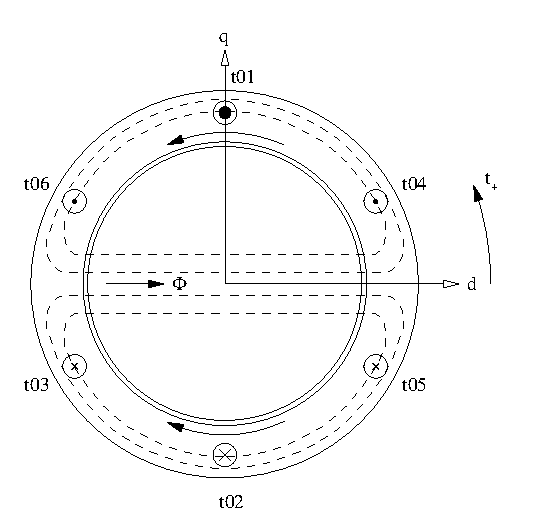
\includegraphics[height=6.2cm]{figs/f_mmf_rotationa.eps}
\end{psfrags}%}
  \hfill
  \subfloat[$t=t_1$\label{fig:mmfrot1}]{
  \begin{psfrags}%
\psfragscanon

% text strings:
\psfrag{t01}{+1}
\psfrag{t02}{-1}
\psfrag{t03}{+3}
\psfrag{t04}{-3}
\psfrag{t05}{+2}
\psfrag{t06}{-2}
\psfrag{t07}[bc]{$t=0$}
\psfrag{t08}[bc]{$t=t_1$}

% Figure:
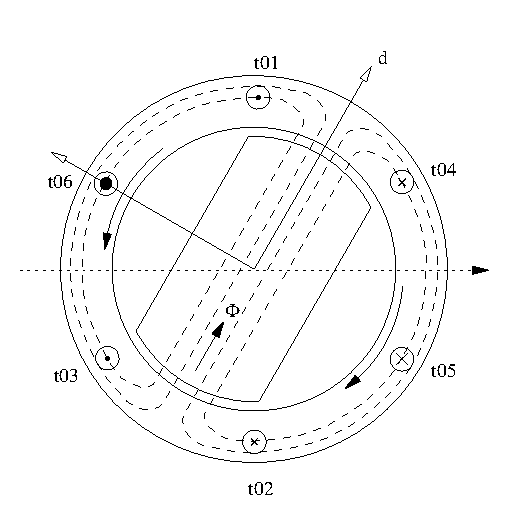
\includegraphics[height=6cm]{figs/f_mmf_rotationb.eps}
\end{psfrags}%}
  \caption[Rotation of the resultant mmf]{Rotation of the resultant mmf by displacing~%
  the three positive coil sides along the stator periphery}
  \label{fig:rotating_wave}
\end{figure}

\subsection{Definition of the mmf envelope functions}\label{subsec:mmf_def}
As time continues, any point on the standing wave will have a minimum and maximum value between which it oscillates. If $p_2$ is used as an example, it will be bounded as shown in Fig.~\ref{fig:mmf_2}\subref{fig:mmfrot1}, thus forming an envelope. Similarly, the remaining phases will each form envelope functions. The bounding functions for all the phases are given by
\begin{equation}
  \label{eqn:f_bound}
  f_n(\theta) = \hat{F_n}\cos\left[\theta+\frac{2\pi}{m}(n-1) \right], 
  \quad 1 \leq n \leq m
\end{equation}
and the mmf of any of the phases will be bounded, i.e. 
\begin{equation}
  -\left|f_n(\theta)\right| \leq F_n(\theta ,t) \leq \left|f_n(\theta)\right|
\end{equation}

\subsection{Phase belt definition}\label{subsec:phasebelt_def}
The mmf envelope functions in section \ref{subsec:mmf_def} allow the definition of the phase belt in a unique way, which make it possible to allocate the stator slots that belong to a phase before the coil sides are assigned. 
\begin{defth}
In general, the interval $\left\langle \theta_1,\theta_2 \right\rangle$ for which any of the $m$ bounding functions in \eqref{eqn:f_bound} is greater than the remaining $(m-1)$ functions is defined as a phase belt, i.e. 
\begin{equation}
 \left|f_i(\theta)\right| > \left|f_n(\theta)\right|, \quad
 \begin{cases}
   1 \leq n \leq m \\
   n \neq i
 \end{cases}
\end{equation}
and the interval $\left\langle \theta_1,\theta_2 \right\rangle$ spans $\frac{2\pi}{2m}$ radians. 
\end{defth}
A useful parameter to define is the total number of phase belts around the air gap periphery, i.e. 
\begin{equation}
  \label{eqn:Np}
  N_p = \frac{2\pi p}{\left(\frac{2\pi}{2m}\right)}=p\cdot2m
\end{equation}
and means that the phase belt sequence (for three phases) given in \eqref{eqn:phasebelt_sequence} repeat itself $p$ times around the air gap periphery.

\subsection{Higher order harmonics}
A similar procedure as for the working harmonic can be used to derive the direction of rotation for the higher order harmonics. The decomposition of the air gap mmf means that the resultant mmf is the sum of an infinite number of rotating waves. The general expression for harmonic order (for three phases and six phase belts) of the air gap mmf harmonics is
\begin{equation}
  \label{eqn:harm_oder}
  \nu = 1+6g \quad g=0,\mp1,\mp2,\ldots
\end{equation}
and the speed of rotation is given by 
\begin{equation}
  \omega_{\nu} = \frac{\omega}{\nu}
\end{equation}
A positive value of $\nu$ means that the harmonic is rotating counter-clockwise and a negative $\nu$ means it rotates clockwise. This convention is valid for the coil arrangement as given in Fig.~\ref{fig:mmf_2}(a) and the currents in \eqref{eqn:3ph_i}. The rotation speed is proportional to the inverse of the harmonic order.
%\chapter{Matrix representation of a winding}
In this section it will be shown that the winding layouts can be represented by means of two matrices. The first matrix will contain information on the ingoing coil sides of the coils while the second matrix will be that of the outgoing coil sides. The matrices are referred to as $\mathbf{M_1}$ and $\mathbf{M_{2}}$ for the ingoing and outgoing coil sides respectively. Both matrices have $n$ columns and $m$ rows. In addition, the number of columns equals the number of stator slots and the rows are equal to the number of phases, thus $m=m$\footnote{It is typical in mathematics that the number of rows is represented by $m$. Equally the number of phases of an electrical machine is also represented by $m$. Furthermore, $m_{11}$ is a matrix element while $m$ is the number of phases.} and $n=Q_s$. The matrices can be expressed as
\begin{equation}
  \label{eqn:M_matrix}
  \mathbf{M}_k = \left[
  \begin{array}{cccc}
     m_{11} & m_{12} & \ldots & m_{1n}\\
     m_{21} & m_{22} & \ldots & m_{2n}\\
     \vdots & \vdots & \ddots & \vdots\\
     m_{m1} & m_{m2} & \ldots & m_{mn}\\
  \end{array} \right]
  \qquad \mbox{where} \qquad
  \begin{cases}
     k = 1,2\\
     m_{ij} \in \left\{-1,0,1\right\}\\
  \end{cases}
\end{equation}
and depends on the winding layout. In the rest of this section an algebraic method is derived to determine the matrix elements. The variables $n_1$ and $n_2$ are integers and will be used as loop variables later on in this chapter where the algorithm flowchart is explained. The subscripts $1$ and $2$ refer to the outer and inner loop respectively. 

\section{Slot vector}
For assigning the $Q_s$ slots to phase belts, the peripheral slot angle $\alpha$ needs to be defined in terms of the slot pitch $\tau_s$. If the slots have a regular distribution the angle between any two adjacent slots equals $\tau_s$. In the case of irregular distributed slots the average slot pitch will equal $\tau_s$. A regular and irregular distribution are shown in Fig.~\ref{fig:f_slotstar}. A vector is assigned to the centre of each stator slot. The exponential representation\footnote{Also known as Euler's formula, \cite{REF-01047}.} of a vector is used, i.e.
\begin{equation} 
  e^{\i\nu \alpha}=\cos(\nu \alpha)+\i\sin(\nu \alpha)
\end{equation}
The variables $\nu$ and $\alpha$ are the harmonic order and slot peripheral angle respectively. All the vectors as shown in Fig.~\ref{fig:f_slotstar} are represented as a column matrix $\mathbf{v}_{\nu}$. The number of rows is equal to the number of slots, i.e.
\begin{equation}
  \label{eqn:slot_vector}
  \mathbf{v}_{\nu}=\left[
                         e^{\i\nu\alpha_1} 
                         \: 
                         e^{\i\nu\alpha_{n_2}} 
                         \:
                         \ldots 
                         \: e^{\i\nu\alpha_{Q_s}}
                    \right]^{T}
   \qquad 1 \leq n_2 \leq Q_s                 
\end{equation}
where
\begin{equation}
  \label{eqn:slot_alpha}
  \alpha_{n_2} = \left\{ \begin{array}{lll}
    \tau_s\left(n_2-1\right) && n_2 \;\text{odd}\\
    \alpha_{n_2-1}+x\tau_s & 0<x<2 & n_2\;\text{even}
  \end{array} \right.
  \quad
  1 \leq n_2 \leq Q_s
\end{equation}
where the $\alpha$ accounts for both regular and irregular distributed stator slots. Setting $\nu=p$ means that the electrical slot angles\footnote{The electrical and mechanical slot have the following relationship: $\theta_e=p \theta_m$} for the working harmonic are obtained. 
\begin{figure}
  \centering
  \fontsize{8}{0}\selectfont
  \subfloat[Regular distribution $x=1$\label{fig:slotstara}]{
  \begin{psfrags}%
\psfragscanon

% text strings:
\psfrag{t01}{1}
\psfrag{t02}{$Q_s$}
\psfrag{t03}{$2\tau_s$}
\psfrag{t04}{$x\tau_s$}

% Figure:
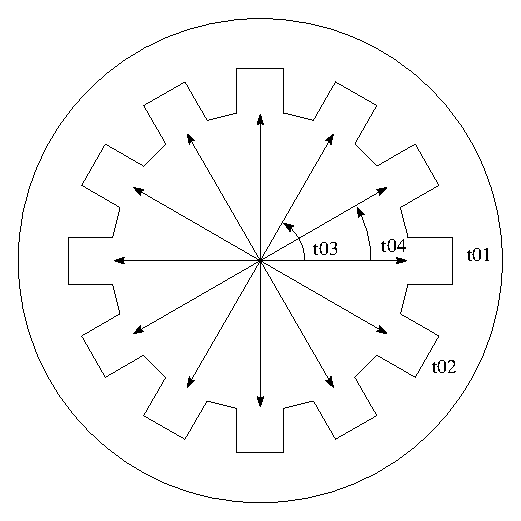
\includegraphics[height=6.5cm]{figs/f_slotstara.eps}
\end{psfrags}%
}
  \hfill
  \subfloat[Irregular distribution $0<x<2$\label{fig:slotstarb}]{
  \begin{psfrags}%
\psfragscanon

% text strings:
\psfrag{t01}{1}
\psfrag{t02}{$Q_s$}
\psfrag{t03}{$2\tau_s$}
\psfrag{t04}{$x\tau_s$}

% Figure:
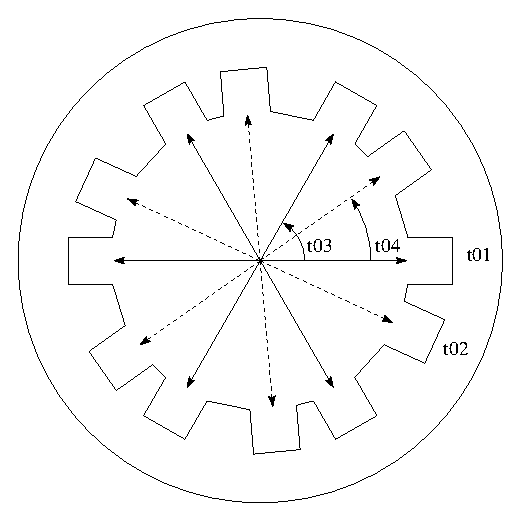
\includegraphics[height=6.5cm]{figs/f_slotstarb.eps}
\end{psfrags}%
}
  \caption{Star of slots}
  \label{fig:f_slotstar}
\end{figure}

\subsection{Phase belt constraint}
The phase belt constraint is used to determine the matrix elements $m_{ij}$ in \eqref{eqn:M_matrix}. From the slot angle $\alpha$ in \eqref{eqn:slot_vector} the corresponding electrical angle $\theta_e$ is obtained. A stator slot is assigned to the phase belt if the following constraint is true:
\begin{equation}  
 \label{eqn:phase_belt_constraint}
  \theta_1 \leq \theta_e  < \theta_2
  \quad
  \begin{cases}
    \left.
      \begin{array}{l}
        \theta_1 = \frac{2\pi}{2m}\left(n_1-1\right) \\
        \theta_2 = \frac{2\pi}{2m}n_1 \\
        1 \leq n_1 \leq N_p \\      
      \end{array}
    \right\} 
    \quad \mbox{phase belt boundaries} \\
    \left.
      \begin{array}{l}
        \theta_e = p\alpha_{n_2} \\
        1 \leq n_2 \leq Q_s \\      
      \end{array}    \right\} 
    \quad \mbox{electrical slot angle} \\
  \end{cases}
\end{equation} 
The phase belt constraint as given in \eqref{eqn:phase_belt_constraint} is characterised by the phase belt boundaries and the electrical slot angle, which are summerised as follows:
\begin{description}
  \item[Phase belt boundaries:] The total number of phase belts around the air gap~%
  periphery is given by \eqref{eqn:Np}. Each of the phase belts is bounded the by~%
  the angles $\theta_1$ and $\theta_2$.
  \item[Electrical slot angle:] The electrical slot angle is obtained by multiplying~%
  the peripheral slot angle in \eqref{eqn:slot_alpha} by the pole pair number. If~%
  the electrical angle for a given slot lies within the phase belt boundaries, it~%
  belongs to that phase belt.   
\end{description}
In order to assign the slot to a phase, it is necessary to know to which phase a given phase belt belongs. The phase can be determined in terms of the given phase belt number $n_1$ and the number of phases, i.e.
\begin{equation}
  \label{eqn:phase_belt_number}
  k = \mbox{mod}(n_1,2m)
  \quad
  \begin{cases}
    1 \leq n_1 \leq \ N_p \\
    2m \ \mbox{if} \ \mbox{mod}(n_1,2m)=0 \\
  \end{cases}
  \quad
  1\leq k \leq 2m
\end{equation}  
The value of $k$ as calculated in \eqref{eqn:phase_belt_number} corresponds to the phase belt number. Therefore, if the number of a given phase belt is known, the corresponding phase and its sign are calculated as follows:
\begin{equation}
  \label{eqn:phase_belt_number_2}
  \begin{aligned}
  \mbox{phase}&= 
    \left\{
    \begin{array}{ll}
      k   & k \leq m\\
      k-m & k > m
    \end{array}
    \right.
    \\
  \mbox{sign}&=(-1)^{(k-1)} 
  \end{aligned}
\end{equation}  
If $m=3$ and $p=1$ the number of phase belts equals 6. Applying \eqref{eqn:phase_belt_number} and \eqref{eqn:phase_belt_number_2} will result in the phase belt sequence as given in \eqref{eqn:phasebelt_sequence}. 

\subsection{Algorithm flowchart}
The explanation of the algorithm is accompanied by the flowchart in Fig.~\ref{fig:flowchart} and greatly simplifies the understanding. For convenience the relevant equations or tables are included which makes it easier to follow the description. The algorithm only applies to symmetrical windings and the three major parts are summerised as follows:
\begin{description}
  \item[Outer loop:] The outer loop of the flowchart is used for the total number of phase belts as given in \eqref{eqn:Np}. The loop index $n_1$ (in the range $1\leq n_1 \leq N_p$) is used to calculate the given phase belt boundaries $\theta_1$ and $\theta_2$ as given in \eqref{eqn:phase_belt_constraint}. Since the $2m$ phase belts repeat themselves along the air gap periphery, the actual phase belt number $k$ in the phase belt sequence can be determined from $n_1$ as given in \eqref{eqn:phase_belt_number} and \eqref{eqn:phase_belt_number_2}.
  \item[Inner loop:] The inner loop has $n_2$ as index and is used to calculate the electrical angle for a given slot. If a slot is already assigned to a phase belt, the winding matrix will have an entry in the set $\{-1,1\}$. In this case the loop is skipped.   
  \item[Phase belt constraint:] This is the key step to allocate a stator slot. If the electrical angle lies within the phase belt boundaries, it belongs to the given phase belt. The row and column number for the ingoing matrix $\mathbf{M_1}$ are determined from the inner loop index $n_2$ and the given phase belt number. The row number for $\mathbf{M_2}$ is the same as for $\mathbf{M_1}$ and the column number is obtained from the coil pitch $y_d$.
\end{description}
The assignment of the stator slots as offered in this dissertation is unique and not presented in this way by any of the references consulted. 
\begin{figure}
  \centering
  \fontsize{9}{10}\selectfont
  \begin{psfrags}%
\psfragscanon

% text strings:
\psfrag{t01}[bc]{$n_1 = 1,N_p$}
\psfrag{t02}[bc]{$\theta_1, \; \theta_2$}
\psfrag{t04}[bc]{$k=f(n_1,m)$}
\psfrag{t05}[bc]{$n_2 = 1,Q_s$}
\psfrag{t07}[bc]{$\theta_1 \leq \theta_e < \theta_2$}
\psfrag{t08}[bc]{$i=f(k)$ and $h=-1^{(k-1)}$}
\psfrag{t09}[bc]{$\mathbf{M}_{1,ij}=h \quad j=n_2$}
\psfrag{t10}[bc]{$\mathbf{M}_{2,ij}=-h \quad j=f(n_2,y_d)$}
\psfrag{t11}[bc]{$n_2=Q_s$?}
\psfrag{t12}[bc]{$n_1=N_p$?}
\psfrag{t14}[bc]{Start}
\psfrag{t15}[bc]{$\mathbf{M}_{ij} \in \left\{-1,1\right\}$}

\psfrag{t16}[bc]{$\mbox{mod}(n_2,2)=0$}
\psfrag{t161}[bc]{\eqref{eqn:modn20}}
\psfrag{t18}[br]{Slots}
\psfrag{t19}[br]{Phase belts}

\psfrag{t20}[bc]{$\theta_e = f(\tau_s)$}
\psfrag{t21}[bl]{\eqref{eqn:phase_belt_number}}

\psfrag{t23}[bl]{\eqref{eqn:Np}}

\psfrag{t13}[bc]{End}
\psfrag{t29}[br]{Section \ref{sec:m_assignment}}
\psfrag{t30}[bl]{\eqref{eqn:phase_belt_constraint}}
\psfrag{t32}[bl]{\eqref{eqn:matrix_element}}
\psfrag{t33}[bc]{y}
\psfrag{t34}[bc]{n}

% Figure:
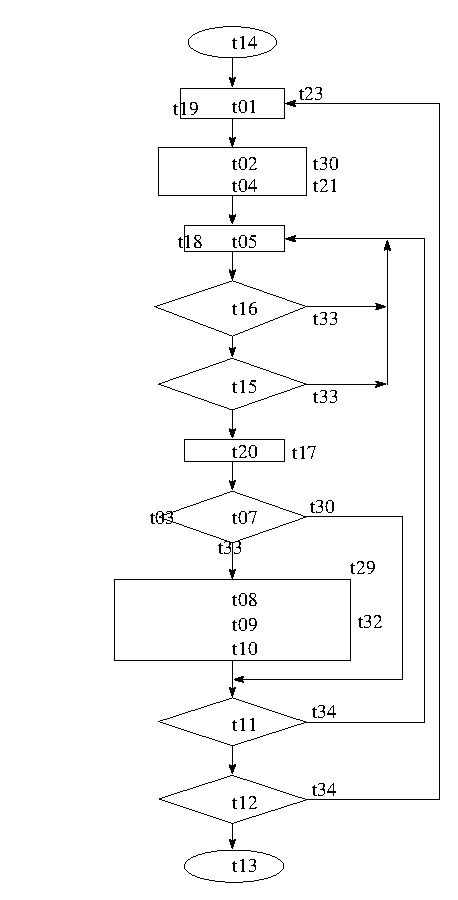
\includegraphics[width=0.55\textwidth]{figs/f_flowchart.eps}
\end{psfrags}%
  \caption{Flowchart to allocate the stator slots}
  \label{fig:flowchart}
\end{figure}

\subsection{Matrix element assignment}\label{sec:m_assignment}
Once the phase belt constraint is fulfilled, the slot is allocated and the next step is to assign one of the values in the set given in \eqref{eqn:M_matrix}. Actually only the sign needs to be determined. Since the phase belt sequence is alternating, the sign can be obtained from the phase belt itself. Following the flowchart through to the point where the test is performed, it is noticed that the matrix column number for $\mathbf{M}_1$ is given by the loop index variable $n_2$. The entry has the value  $(-1)^{(k-1)}$, where $k$ is given in \eqref{eqn:phase_belt_number}. The determination of the row, column and matrix element are summerised as follows\footnote{The method was only tested for $m=3,5,7,\ldots$}: 
\begin{equation}
  \label{eqn:matrix_element}
  \begin{aligned}
  i &= 
  \left\{ 
    \begin{array}{ll}
      k   & k \leq m\\
      k-m & k > m
    \end{array}
    \qquad 
  \right\}
  \mbox{row number}
  \\
  h &= (-1)^{(k-1)} 
  \quad 
  \mbox{matrix element sign} 
  \\
  j &= 
  \left\{ 
    \begin{array}{ll}
      n_2+y_d   & n_2+y_d \leq Q_s \\
      \mbox{mod}\bigl((n_2+y_d),Q_s\bigr) & n_2+y_d > Q_s
    \end{array} 
    \quad
  \right\}
  \mbox{column number}
  \end{aligned}
\end{equation}

\section{Properties of the winding matrix}
Presenting the winding in matrix form is very compact and has advantages in machine analysis. The matrix contains all the information of the winding arrangement in the stator slots. This allows the construction of the voltage phasor which is necessary to calculate the winding factor. In addition, the slot mmf can be obtained from the column data. The properties of the matrix are summerised as follows:
\begin{itemize}
  \item if the winding is symmetrical, the number of assigned elements in all~%
  the rows are equal;
  \item the number of columns is equal to the number of stator slots;
  \item the number of rows is equal to the number of phases;
  \item for a single layer winding there is only one nonzero element in a column;
  \item a double layer winding has two nonzero elements in a row; and
  \item the matrix is valid for both a fixed and variable slot pitch.
\end{itemize}
In the rest of this section the winding matrix is used to calculate the winding factor and the slot mmf.

\subsection{Winding factor}
With $\mathbf{M}_1$ and $\mathbf{M}_2$ assigned, the winding factor for any harmonic can be calculated as the product between the matrices and the slot vector as given in \eqref{eqn:slot_vector}. This means that a row of the winding matrix is multiplied by the slot vector column matrix. The matrix product means that all the vectors belonging to the same phase are added and for the case $\nu=p$ equals\footnote{$j$ as imaginary number and $j$ as column number can be confusing.}
\begin{equation}
  \label{eqn:m1_m2_exp}
  c_{i1}e^{\i p\alpha_1}+c_{i2}e^{\i p\alpha_2}+\ldots+
  c_{iQ_s}e^{\i p \alpha_{Q_s}} = \sum_{j=1}^{Q_s}c_{ij}e^{\i p\alpha_k}
  \quad \mbox{where} \quad
  c_{ij} = m_{1,ij}+m_{2,ij}
\end{equation}
If the slot vector does not belong to the current phase, the coefficient
\begin{equation} 
  \left(m_{1,ij}+m_{2,ij}\right)
\end{equation} 
is zero. Furthermore, the product should be normalised. Since the total number of vectors is related to the coils per phase it should be multiplied by $\left(2\frac{Q_c}{m}\right)^{-1}$, i.e.
\begin{equation}
  \label{eqn:winding_factor}
  \xi_{\nu} = \frac{m}{2Q_c}
  \Bigl[
    \mathbf{M}_1\mathbf{v_{\nu}}+\mathbf{M}_2\mathbf{v_{\nu}}
  \Bigr], 
  \quad \in \mathbb{C}
\end{equation}
The result \eqref{eqn:winding_factor} present the winding factor as a complex number and the absolute value is to be used as a reduction factor for the sinusoidally induced voltage in \eqref{eqn:ui}. Writing $\xi_{\nu}$ as
\begin{equation}
  \xi_{\nu} = a_{\nu}+\i b_{\nu}
\end{equation}
the phase angle is calculated as 
\begin{equation}
  \theta_{\nu} = \arctan\left(\frac{b_{\nu}}{a_{\nu}}\right)
\end{equation}
The phase angle (in electrical radians) gives information on the position of the winding axes\footnote{The winding axes in the present dissertation refer to the current anti-node axis and the magnetic axis.} relative to the first slot. The two winding axes associated with each phase are called
\begin{itemize}
  \item the current sheet anti-node axis and
  \item the magnetic axis
\end{itemize}
of the winding. A positive phase angle means that both winding axes have moved clockwise with respect to the first slot. The winding axes are a very import quantities in machine design. When the machine is supplied with a source, a rotating magnetic flux wave is generated. This reacts with the flux generated by the flux of the permanent magnets on the rotor. In order to control the resultant flux, it is necessary to know the exact position of the winding axes.  

\begin{equation}\label{eqn:dft}
  X(k) = \sum_{j=1}^N \; x(j) \; e^{-(j-1)(k-1)\theta i}
  \qquad
  \xi(\nu) = \sum_{k=1}^{Q_s}c_{ik}e^{jp\alpha_k}
\end{equation}

\subsection{Current sheet anti-node axis}\label{subsec:current_sheet}
Equation \eqref{eqn:F_theta_t_1} describes the space fundamental component of the mmf produced by the current in phase 1. It can be seen as the mmf wave produced by a finely divided sinusoidally distributed current sheet placed on the inner periphery of the stator. The position of the anti-node with maximum deviation is given by $\theta_{an}$. The relative position of $\theta_{an}$ with respect to the first slot is given by
\begin{equation}
  \label{eqn:theta_an}
  \theta_{an_{\nu}} = -
  \frac{\theta_{\nu}}{p}
\end{equation} 

\subsection{Magnetic axis}\label{subsec:magnetic_axis}
The axis along which the flux is directed when current is flowing in the coil, is defined as the magnetic axis. This is the same position where the current sheet has a node. The relative position of the magnetic axis $\theta_m$ with respect to the first slot is given by
\begin{equation}
  \label{eqn:theta_m}
  \theta_{m_{\nu}} = -
  \frac{\left(\theta_{\nu}+\frac{\pi}{2}\right)}{p}
\end{equation} 
The winding magnetic axis lags the current sheet anti-node axis by $\frac{\pi}{2}$
radians.

\subsection{Slot mmf}\label{subsec:slot_mmf}
The amp\`ere-turns in each slot can be obtained from the matrix winding columns. Both the matrices $\mathbf{M_1}$ and $\mathbf{M_2}$ contain the coil side information for the ingoing and outgoing coil sides respectively. The total amp\`ere-turns of a coil side is the product of its value in the winding matrix with the number of coil turns $N_t$. The direction of the current is given by the sign of the element. Therefore to get the total amp\`ere-turns in the slot, the amp\`ere-turns of the coil sides must be added. For a three-phase winding the slot mmf $F_{slot}$ of the $k^{th}$ slot is calculated as  
\begin{equation}
  \label{eqn:slot_mmf}
  \begin{aligned}
  F_{slot,k} &= N_t i_1(m_{1,1k}+m_{2,1k})+
                N_t i_2(m_{1,2k}+m_{2,2k})+
                N_t i_3(m_{1,3k}+m_{2,3k}) \\
             &= N_t\sum_{n=1}^{3}i_n \left(m_{1,nk}+m_{2,nk}\right) 
  \end{aligned}
\end{equation}

\section{Examples}
The derived theory presented in this chapter is now illustrated by means of examples. The examples are summerised as follows:
\begin{description}
  \item[Winding factor tables:] The winding factors for different slot and pole pair combinations are calculated for single and double layer non-overlapping windings. The results presented are used to derive an expression to find the feasible range for the number of pole pairs, given the number of stator slots. 
  \item[Slot mmf and current sheet:] The prototype stator with 30 slots is used as an example. By choosing different pole pair numbers, it is shown how to obtain both a single and double layer winding. In each case a non-overlapping and overlapping winding are explained.
\end{description}
  
\subsection{Winding factor table}\label{subsec:wind_fac_table}
The results are given in Tab.~\ref{tab:xi_single} Tab.~\ref{tab:xi_double} for single and double layer non-overlapping windings respectively. Only those slot and pole combinations for which the winding factor is greater than or equal to $\frac{\sqrt{3}}{2}$ are given. Those combinations that do not fulfill the condition in \eqref{eqn:feasibility} are marked as not applicable. Presenting the winding factors in a table is helpful to identify the relationship between the number of stator slots and the number of poles which results in the best combinations. Only the winding factors for the working harmonic are presented. 

The winding factors for single windings are calculated for pole pairs in the range from 4 to 28, whereas the number of stator slots range from 12 to 84. Although the focus in the present dissertation is on single layer non-overlapping windings, the winding factors for double layer windings are given as well. The winding factors are calculated for pole pairs in the range from 4 to 16, whereas the number of stator slots ranges from 12 to 48.
\begin{table}[htbp]
  \caption{$\xi_p \times \num{e-3}$ for single layer non-overlapping windings}
  \label{tab:xi_single}
  \centering
   \begin{tabular}
  	{|l||c|c|c|c|c|c|c|c|c|c|c|c|c|}\cline{2-14}
  	\multicolumn{1}{c}{}& \multicolumn{13}{|c|}{$Q_s$}
  	\\\hline
  	$p$&12 &18 &24 &30 &36 &42 &48 &54 &60 &66 &72 &78 &84  \\\hline
  	4  &866&   &   &   &   &   &   &   &   &   &   &   &    \\
  	5  &966&   &   &   &   &   &   &   &   &   &   &   &    \\
  	6  &na &866&   &   &   &   &   &   &   &   &   &   &    \\
  	7  &966&902&   &   &   &   &   &   &   &   &   &   &    \\
  	8  &866&945&866&   &   &   &   &   &   &   &   &   &    \\
  	9  &   &na &na &   &   &   &   &   &   &   &   &   &    \\
  	10 &   &945&966&866&   &   &   &   &   &   &   &   &    \\
  	11 &   &902&958&874&   &   &   &   &   &   &   &   &    \\
  	12 &   &866&na &na &866&   &   &   &   &   &   &   &    \\
  	13 &   &   &958&940&870&   &   &   &   &   &   &   &    \\
  	14 &   &   &966&950&na &866&   &   &   &   &   &   &    \\
  	15 &   &   &na &na &966&na &   &   &   &   &   &   &    \\
  	16 &   &   &866&950&na &na &866&   &   &   &   &   &    \\
  	17 &   &   &   &940&956&na &859&   &   &   &   &   &    \\
  	18 &   &   &   &na &na &na &na &866&   &   &   &   &    \\
  	19 &   &   &   &866&956&na &907&na &   &   &   &   &    \\
  	20 &   &   &   &866&na &na &966&na &866&   &   &   &    \\
  	21 &   &   &   &   &966&na &na &na &na &   &   &   &    \\
  	22 &   &   &   &   &na &na &958&na &954&866&   &   &    \\
  	23 &   &   &   &   &870&na &956&na &893&na &   &   &    \\
  	24 &   &   &   &   &866&na &na &na &na &na &866&   &    \\
  	25 &   &   &   &   &   &na &956&na &966&na &848&   &    \\
  	26 &   &   &   &   &   &na &958&na &na &na &870&866&    \\  
  	27 &   &   &   &   &   &na &na &na &na &na &na &na &    \\  
  	28 &   &   &   &   &   &866&966&na &na &na &na &na &866 \\\hline  	  
  \end{tabular}
\end{table}
 
\begin{table}[htbp]
  \caption{$\xi_p \times \num{e-3}$ for double layer non-overlapping windings }
  \label{tab:xi_double}
  \centering
  \begin{tabular}
  	{|l||c|c|c|c|c|c|c|c|c|c|c|c|c|}\cline{2-14}
  	\multicolumn{1}{c}{}& \multicolumn{13}{|c|}{$Q_s$}
  	\\\hline
  	$p$&12 &15 &18 &21 &24 &27 &30 &33 &36 &39 &42 &45 &48  \\\hline
  	4  &866&   &   &   &   &   &   &   &   &   &   &   &    \\
  	5  &930&866&   &   &   &   &   &   &   &   &   &   &    \\
  	6  &na &na &866&   &   &   &   &   &   &   &   &   &    \\
  	7  &930&950&900&866&   &   &   &   &   &   &   &   &    \\
  	8  &866&950&950&890&866&   &   &   &   &   &   &   &    \\
  	9  &   &na &na &na &na &866&   &   &   &   &   &   &    \\
  	10 &   &866&950&950&930&880&866&   &   &   &   &   &    \\
  	11 &   &   &900&950&950&920&870&866&   &   &   &   &    \\
  	12 &   &   &866&na &na &950&na &na &866&   &   &   &    \\
  	13 &   &   &   &890&950&950&940&900&870&866&   &   &    \\
  	14 &   &   &   &866&930&950&950&930&900&860&866&   &    \\
  	15 &   &   &   &   &na &950&na &na &930&na &na &866&    \\
  	16 &   &   &   &   &866&920&950&950&950&920&890&860&866 \\\hline  	  
  	\end{tabular}
\end{table}

From the results in Tab.~\ref{tab:xi_single} and Tab.~\ref{tab:xi_double} the number of slots per pole and phase which results in a winding with suitable winding factors is given by
\begin{equation}
  \frac{1}{4} \leq q \leq \frac{1}{2}
\end{equation}
The result is the same as presented by \cite{REF-00754} and \cite{REF-00756}. Using this result, the range of pole pairs for a given number of slots can be expressed as follows:
\begin{equation}
  \frac{Q_s}{m} \leq p \leq \frac{2Q_s}{m}
  \quad
  \left\{
  \begin{array}{ll}
  Q_s \in \left\{6,12,18,\ldots\right\} & \mbox{single layer}\\
  \:  & \: \\
  Q_s \in \left\{3,6,9,\ldots\right\} & \mbox{double layer}\\
  \end{array}
  \right.
\end{equation} 

\subsection{Slot mmf and current sheet}
This section entails examples of overlapping and non-overlapping windings with 30 stator slots. The classification parameters $q$, $q_c$ and $y_d$ (as given in Tab.~\ref{tab:Example_table}) are used to classify the windings according to the scheme in Fig.~\ref{fig:classification}. Additionally, for the selected number of pole pairs the winding factor, slot mmf and current sheet are calculated. It is important to mention that the choice of the position of the reference slot will determine the rotation direction of the resulting rotating field. It is desirable to have a field rotating in a counter-clockwise direction, since this is the positive direction in a polar coordinate system. To achieve this, the stator is rolled flat with the top part of the slots facing upwards. 
\begin{table}[htbp]
  \caption{Different pole pair combinations with $Q_s = 30$}
  \label{tab:Example_table}
  \centering  
   \begin{tabular}{ccccccccccccccccc}
    \toprule
  	$Q_s$ &$p$ &$Q_c$ &$n_l$& $y_p$ &$y_d$ &$q$ &$q_c$ & $Q_b$ & $t$ &
  	$\xi_p$ &$\xi_{5p}$ &$\xi_{7p}$ &Figure
  	\\
  	\midrule
  	30    &10  &15  &1   &$\frac{3}{2}$   &1   &$\frac{1}{2}$ &  $\frac{1}{4}$& 6 & 5 &
  	0.866   &0.866      &0.866      &%
  	\ref{fig:Main_non-overlapping_single}\subref{fig:f_Qs30_p10_1}
  	\\
  	30    &10  &30  &2    &$\frac{3}{2}$  &1   &$\frac{1}{2}$ &  $\frac{1}{2}$ & 3&10 &
  	0.866   &0.866      &0.866      &%
  	\ref{fig:Main_non-overlapping_double}\subref{fig:f_Qs30_p10_2}
  	\\    
  	30    &5   &15  &1    &3 &3  &1 &  $\frac{1}{2}$ & 6 & 5  &
  	1.0     &1.0        &1.0        &%
  	\ref{fig:Main_single_overlapping}\subref{fig:f_Qs30_5_1}
  	\\
  	30    &5   &30  &2    &3 &3  &1 &  1 & 6 & 5  &
  	1.0     &1.0        &1.0        &%
  	\ref{Main_double_overlapping}\subref{fig:f_Qs30_p5_2}   
  	\\
  	\bottomrule  	  
   \end{tabular}
\end{table} 

\subsubsection{Single layer non-overlapping}
Fig.~\ref{fig:Main_non-overlapping_single}\subref{fig:single_layer} shows an illustration of a single layer non-overlapping winding. There is only one coil side in each stator slot and the slot pitch could be either regular or irregular. An irregular slot pitch means that the coil pitch can be varied to improve the winding factor. Depending on the design criteria, it can also be used to improve the torque ripple. Since the outgoing coils are given by the coil pitch $y_d$, only every second slot needs to be assigned to a phase belt.  

The example chosen is that of the prototype machine with 30 slots and 10 pole pairs. 
From Tab.~\ref{tab:Example_table} the values for $q$ and $q_c$ are $\frac{1}{2}$ and $\frac{1}{4}$ respectively. The basic winding is determined using $q_c$ and has one  coil per phase distributed over 4 poles. In total the basic winding has 6 slots. The winding has a sub-harmonic with 5 pole pairs. Since it is a single layer winding the number of coils is half the number of stator slots. The coil pitch equals one and this is a fractional slot winding. For convenience only the basic winding matrix elements for $\mathbf{M_1}$ and $\mathbf{M_2}$ are given as
\begin{equation}
  \mathbf{M_{1,b}} = 
  \begin{pmatrix}
  1&0&0&0&0&0\\
  0&0&1&0&0&0\\
  0&0&0&0&1&0\\
  \end{pmatrix} \
  \mathbf{M_{2,b}} = 
  \begin{pmatrix}
  0&-1&0&0 &0&0 \\
  0&0 &0&-1&0&0 \\
  0&0 &0&0 &0&-1\\
  \end{pmatrix} 
\end{equation}
To obtain the complete winding matrix, the matrix of the basic winding is repeated five times. For the ingoing coil side matrix this means
\begin{equation}
  \mathbf{M_1} = 
  \begin{bmatrix}
  \mathbf{M_{1,b}}&\mathbf{M_{1,b}}&\mathbf{M_{1,b}}&
  \mathbf{M_{1,b}}&\mathbf{M_{1,b}}
  \end{bmatrix}  
\end{equation}
The winding matrix is used to obtain the slot mmf $F_{slot}$ from \eqref{eqn:slot_mmf} as shown in the lower part of~%
Fig.~\ref{fig:Main_non-overlapping_single}\subref{fig:f_Qs30_p10_1}. The dashed line in the mmf plot is the current sheet. In the top part of the figure the winding factors are shown as well. From the figure it is clear that the winding factors are periodic with the number of stator slots. In the example the peripheral slot angle was calculated setting $x=1$ in \eqref{eqn:slot_alpha}. Therefore, this is a regular distribution of the stator slots.
\begin{figure}[htbp]
  \centering
  \fontsize{6}{6}\selectfont
  \subfloat[Winding layout\label{fig:single_layer}]{
  \begin{psfrags}%
\psfragscanon

% text strings:
\psfrag{t01}{{\tiny Constant pitch, $2\tau_s$}}
\psfrag{t02}{{\tiny Variable slot pitch, $x \tau_s$}}
\psfrag{t03}{{\tiny Direction of coil assignment}}
\psfrag{t04}{{\tiny 1}}
\psfrag{t05}{{\tiny 2}}
\psfrag{t06}{{\tiny 3}}
\psfrag{t07}{{\tiny 4}}

% Figure:

\subfloat[Winding layout\label{fig:single_layer}]
  \hfill
  \subfloat[Slot mmf and winding factors\label{fig:f_Qs30_p10_1}]{
  % This file is generated by the MATLAB m-file laprint.m. It can be included
% into LaTeX documents using the packages graphicx, color and psfrag.
% It is accompanied by a postscript file. A sample LaTeX file is:
%    \documentclass{article}\usepackage{graphicx,color,psfrag}
%    \begin{document}% This file is generated by the MATLAB m-file laprint.m. It can be included
% into LaTeX documents using the packages graphicx, color and psfrag.
% It is accompanied by a postscript file. A sample LaTeX file is:
%    \documentclass{article}\usepackage{graphicx,color,psfrag}
%    \begin{document}\input{f_Qs_30_p_10_1}\end{document}
% See http://www.mathworks.de/matlabcentral/fileexchange/loadFile.do?objectId=4638
% for recent versions of laprint.m.
%
% created by:           LaPrint version 3.16 (13.9.2004)
% created on:           12-Nov-2008 21:44:16
% eps bounding box:     17.5 cm x 13.125 cm
% comment:              
%
\begin{psfrags}%
\psfragscanon%
%
% text strings:
\psfrag{s05}[b][b]{{\tiny $\xi_{10}$}}%
\psfrag{s06}[b][b]{{\tiny $\xi_{50}$}}%
\psfrag{s07}[b][b]{{\tiny $\xi_{70}$}}%
\psfrag{s08}[t][t]{{\tiny $\nu$}}%
\psfrag{s09}[b][b]{{\tiny $\xi_{\nu}$}}%
\psfrag{s10}[t][t]{{\tiny Slot number}}%
\psfrag{s11}[b][b]{{\tiny $F_{slot}/\SI{}{A}$}}%
%
% xticklabels:
\psfrag{x01}[t][t]{{\tiny 0}}%
\psfrag{x02}[t][t]{{\tiny 5}}%
\psfrag{x03}[t][t]{{\tiny 10}}%
\psfrag{x04}[t][t]{{\tiny 15}}%
\psfrag{x05}[t][t]{{\tiny 20}}%
\psfrag{x06}[t][t]{{\tiny 25}}%
\psfrag{x07}[t][t]{{\tiny 30}}%
\psfrag{x08}[t][t]{{\tiny 0}}%
\psfrag{x09}[t][t]{{\tiny 10}}%
\psfrag{x10}[t][t]{{\tiny 20}}%
\psfrag{x11}[t][t]{{\tiny 30}}%
\psfrag{x12}[t][t]{{\tiny 40}}%
\psfrag{x13}[t][t]{{\tiny 50}}%
\psfrag{x14}[t][t]{{\tiny 60}}%
\psfrag{x15}[t][t]{{\tiny 70}}%
\psfrag{x16}[t][t]{{\tiny 80}}%
\psfrag{x17}[t][t]{{\tiny 90}}%
%
% yticklabels:
\psfrag{v01}[r][r]{{\tiny -1}}%
\psfrag{v02}[r][r]{{\tiny -0.5}}%
\psfrag{v03}[r][r]{{\tiny 0}}%
\psfrag{v04}[r][r]{{\tiny 0.5}}%
\psfrag{v05}[r][r]{{\tiny 1}}%
\psfrag{v06}[r][r]{{\tiny 0}}%
\psfrag{v07}[r][r]{{\tiny 0.1}}%
\psfrag{v08}[r][r]{{\tiny 0.2}}%
\psfrag{v09}[r][r]{{\tiny 0.3}}%
\psfrag{v10}[r][r]{{\tiny 0.4}}%
\psfrag{v11}[r][r]{{\tiny 0.5}}%
\psfrag{v12}[r][r]{{\tiny 0.6}}%
\psfrag{v13}[r][r]{{\tiny 0.7}}%
\psfrag{v14}[r][r]{{\tiny 0.8}}%
\psfrag{v15}[r][r]{{\tiny 0.9}}%
\psfrag{v16}[r][r]{{\tiny 1}}%
\psfrag{v17}[r][r]{{\tiny 1.1}}%
%
% Figure:

\subfloat[Slot mmf and winding factors\label{fig:f_Qs30_p10_1}]{%
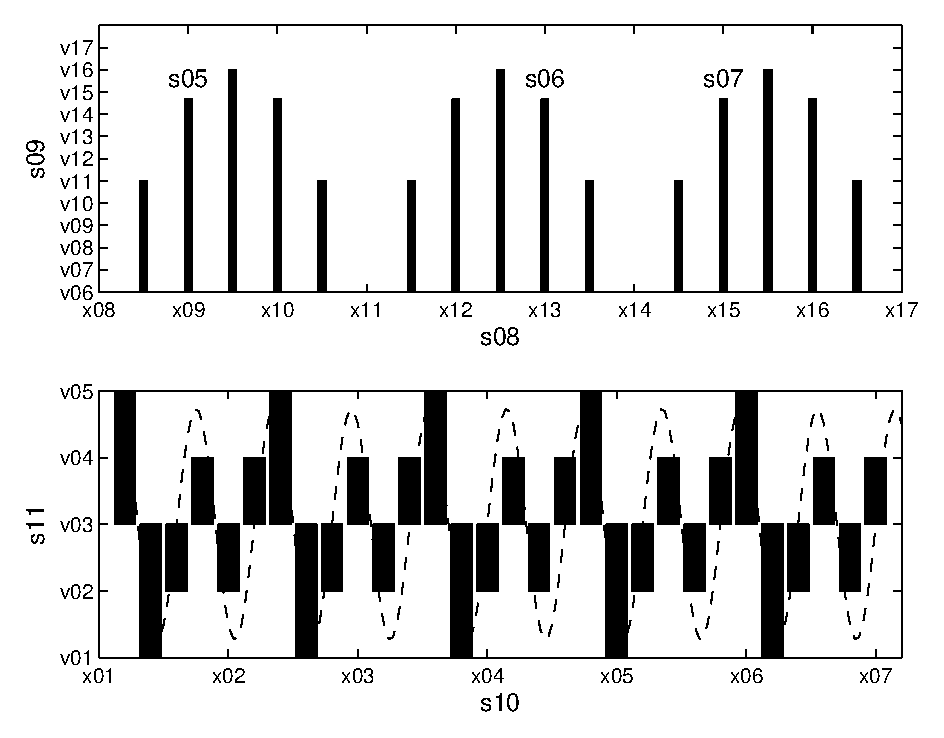
\includegraphics[width=0.9\textwidth]{figs/f_Qs_30_p_10_1.eps}}%
\end{psfrags}%
%
% End f_Qs_30_p_10_1.tex
\end{document}
% See http://www.mathworks.de/matlabcentral/fileexchange/loadFile.do?objectId=4638
% for recent versions of laprint.m.
%
% created by:           LaPrint version 3.16 (13.9.2004)
% created on:           12-Nov-2008 21:44:16
% eps bounding box:     17.5 cm x 13.125 cm
% comment:              
%
\begin{psfrags}%
\psfragscanon%
%
% text strings:
\psfrag{s05}[b][b]{{\tiny $\xi_{10}$}}%
\psfrag{s06}[b][b]{{\tiny $\xi_{50}$}}%
\psfrag{s07}[b][b]{{\tiny $\xi_{70}$}}%
\psfrag{s08}[t][t]{{\tiny $\nu$}}%
\psfrag{s09}[b][b]{{\tiny $\xi_{\nu}$}}%
\psfrag{s10}[t][t]{{\tiny Slot number}}%
\psfrag{s11}[b][b]{{\tiny $F_{slot}/\SI{}{A}$}}%
%
% xticklabels:
\psfrag{x01}[t][t]{{\tiny 0}}%
\psfrag{x02}[t][t]{{\tiny 5}}%
\psfrag{x03}[t][t]{{\tiny 10}}%
\psfrag{x04}[t][t]{{\tiny 15}}%
\psfrag{x05}[t][t]{{\tiny 20}}%
\psfrag{x06}[t][t]{{\tiny 25}}%
\psfrag{x07}[t][t]{{\tiny 30}}%
\psfrag{x08}[t][t]{{\tiny 0}}%
\psfrag{x09}[t][t]{{\tiny 10}}%
\psfrag{x10}[t][t]{{\tiny 20}}%
\psfrag{x11}[t][t]{{\tiny 30}}%
\psfrag{x12}[t][t]{{\tiny 40}}%
\psfrag{x13}[t][t]{{\tiny 50}}%
\psfrag{x14}[t][t]{{\tiny 60}}%
\psfrag{x15}[t][t]{{\tiny 70}}%
\psfrag{x16}[t][t]{{\tiny 80}}%
\psfrag{x17}[t][t]{{\tiny 90}}%
%
% yticklabels:
\psfrag{v01}[r][r]{{\tiny -1}}%
\psfrag{v02}[r][r]{{\tiny -0.5}}%
\psfrag{v03}[r][r]{{\tiny 0}}%
\psfrag{v04}[r][r]{{\tiny 0.5}}%
\psfrag{v05}[r][r]{{\tiny 1}}%
\psfrag{v06}[r][r]{{\tiny 0}}%
\psfrag{v07}[r][r]{{\tiny 0.1}}%
\psfrag{v08}[r][r]{{\tiny 0.2}}%
\psfrag{v09}[r][r]{{\tiny 0.3}}%
\psfrag{v10}[r][r]{{\tiny 0.4}}%
\psfrag{v11}[r][r]{{\tiny 0.5}}%
\psfrag{v12}[r][r]{{\tiny 0.6}}%
\psfrag{v13}[r][r]{{\tiny 0.7}}%
\psfrag{v14}[r][r]{{\tiny 0.8}}%
\psfrag{v15}[r][r]{{\tiny 0.9}}%
\psfrag{v16}[r][r]{{\tiny 1}}%
\psfrag{v17}[r][r]{{\tiny 1.1}}%
%
% Figure:

\subfloat[Slot mmf and winding factors\label{fig:f_Qs30_p10_1}]{%
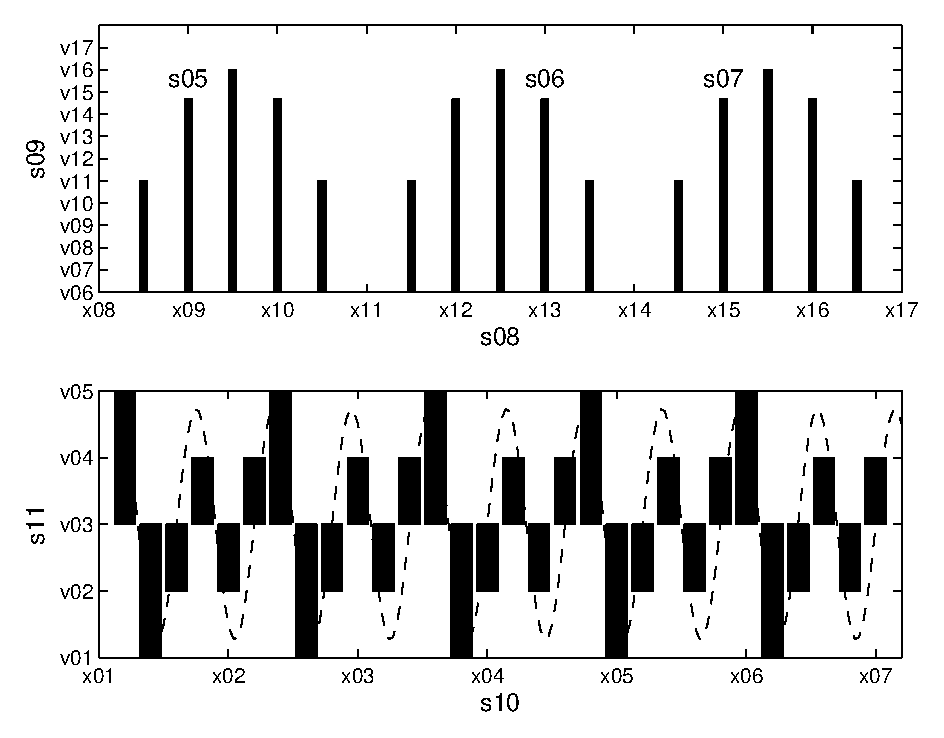
\includegraphics[width=0.9\textwidth]{figs/f_Qs_30_p_10_1.eps}}%
\end{psfrags}%
%
% End f_Qs_30_p_10_1.tex
}
  \caption{Non-overlapping single layer winding}
  \label{fig:Main_non-overlapping_single}
\end{figure}

\subsubsection{Double layer non-overlapping}
Fig.~\ref{fig:Main_non-overlapping_double}\subref{fig:dlw_yd_eq_1} shows a non-overlapping double layer winding. Each stator slot has two coil sides. Moreover, each slot needs to be assigned to a phase belt. 

The prototype stator with 30 slots is used with 10 pole pairs. This is a double layer winding and the number of slots is equal to the number of coils. Both $q$ and $q_c$ and the basic winding has 3 slots. The lowest harmonic has 10 pole pairs which is the same as the working harmonic. Therefore, the winding has no sub-harmonics. The matrix elements of the basic winding are 
\begin{equation}
  \mathbf{M_{1,b}} = 
  \begin{pmatrix}
  1&0&0\\
  0&0&1\\
  0&1&0\\ 
  \end{pmatrix} \
  \mathbf{M_{2,b}} = 
  \begin{pmatrix}
  0 &-1&0\\
  -1&0&0\\
  0&0&-1\\ 
  \end{pmatrix} 
\end{equation}
The winding factors and slot mmf are directly obtained from the winding matrix as shown in Fig.~\ref{fig:Main_non-overlapping_double}\subref{fig:f_Qs30_p10_2}. The current sheet that corresponds to the working harmonic is included.
\begin{figure}[htbp]
  \centering
  \fontsize{6}{6}\selectfont
  \subfloat[Winding layout\label{fig:dlw_yd_eq_1}]{%
  \begin{psfrags}%
\psfragscanon

% text strings:
\psfrag{t01}[bc]{{\tiny $y_d$}}
\psfrag{t02}[bl]{{\tiny Direction of coil assignment}}
\psfrag{t03}{{\tiny 1}}
\psfrag{t04}{{\tiny 2}}
\psfrag{t05}{{\tiny 3}}
\psfrag{t06}{{\tiny 4}}
\psfrag{t07}{{\tiny 5}}

% Figure:

\subfloat[Winding layout\label{fig:dlw_yd_eq_1}]{%
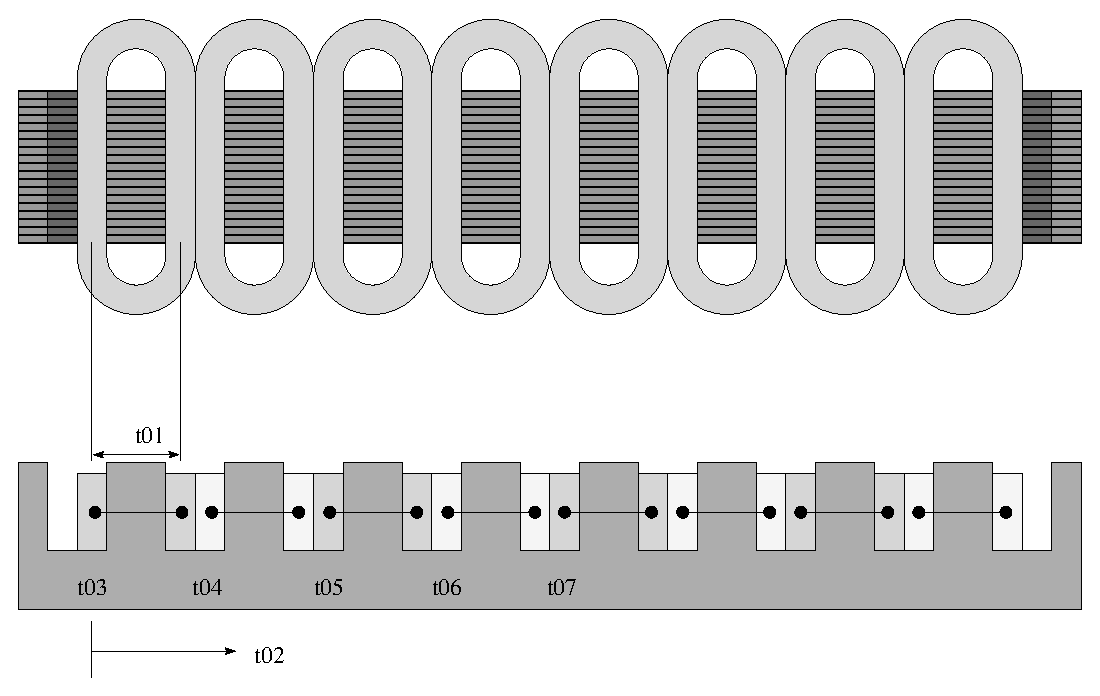
\includegraphics[height=7cm]{figs/f_double_layer_type2.eps}}
\end{psfrags}%
}
  \hfill
  \subfloat[Slot mmf and winding factors\label{fig:f_Qs30_p10_2}]{%  
  % This file is generated by the MATLAB m-file laprint.m. It can be included
% into LaTeX documents using the packages graphicx, color and psfrag.
% It is accompanied by a postscript file. A sample LaTeX file is:
%    \documentclass{article}\usepackage{graphicx,color,psfrag}
%    \begin{document}% This file is generated by the MATLAB m-file laprint.m. It can be included
% into LaTeX documents using the packages graphicx, color and psfrag.
% It is accompanied by a postscript file. A sample LaTeX file is:
%    \documentclass{article}\usepackage{graphicx,color,psfrag}
%    \begin{document}\input{f_Qs_30_p_10_2}\end{document}
% See http://www.mathworks.de/matlabcentral/fileexchange/loadFile.do?objectId=4638
% for recent versions of laprint.m.
%
% created by:           LaPrint version 3.16 (13.9.2004)
% created on:           12-Nov-2008 21:54:09
% eps bounding box:     17.5 cm x 13.125 cm
% comment:              
%
\begin{psfrags}%
\psfragscanon%
%
% text strings:
\psfrag{s05}[b][b]{$\xi_{10}$}
\psfrag{s06}[b][b]{$\xi_{50}$}
\psfrag{s07}[b][b]{$\xi_{70}$}
\psfrag{s08}[t][t]{$\nu$}
\psfrag{s09}[b][b]{$\xi_{\nu}$}
\psfrag{s10}[t][t]{Slot number}
\psfrag{s11}[b][b]{$F_{slot}/\SI{}{A}$}
%
% xticklabels:
\psfrag{x01}[t][t]{0}
\psfrag{x02}[t][t]{5}
\psfrag{x03}[t][t]{10}
\psfrag{x04}[t][t]{15}
\psfrag{x05}[t][t]{20}
\psfrag{x06}[t][t]{25}
\psfrag{x07}[t][t]{30}
\psfrag{x08}[t][t]{0}
\psfrag{x09}[t][t]{10}
\psfrag{x10}[t][t]{20}
\psfrag{x11}[t][t]{30}
\psfrag{x12}[t][t]{40}
\psfrag{x13}[t][t]{50}
\psfrag{x14}[t][t]{60}
\psfrag{x15}[t][t]{70}
\psfrag{x16}[t][t]{80}
\psfrag{x17}[t][t]{90}
%
% yticklabels:
\psfrag{v01}[r][r]{-2}
\psfrag{v02}[r][r]{-1}
\psfrag{v03}[r][r]{0}
\psfrag{v04}[r][r]{1}
\psfrag{v05}[r][r]{2}
\psfrag{v06}[r][r]{0}
\psfrag{v07}[r][r]{0.1}
\psfrag{v08}[r][r]{0.2}
\psfrag{v09}[r][r]{0.3}
\psfrag{v10}[r][r]{0.4}
\psfrag{v11}[r][r]{0.5}
\psfrag{v12}[r][r]{0.6}
\psfrag{v13}[r][r]{0.7}
\psfrag{v14}[r][r]{0.8}
\psfrag{v15}[r][r]{0.9}
\psfrag{v16}[r][r]{1}
\psfrag{v17}[r][r]{1.1}
%
% Figure:
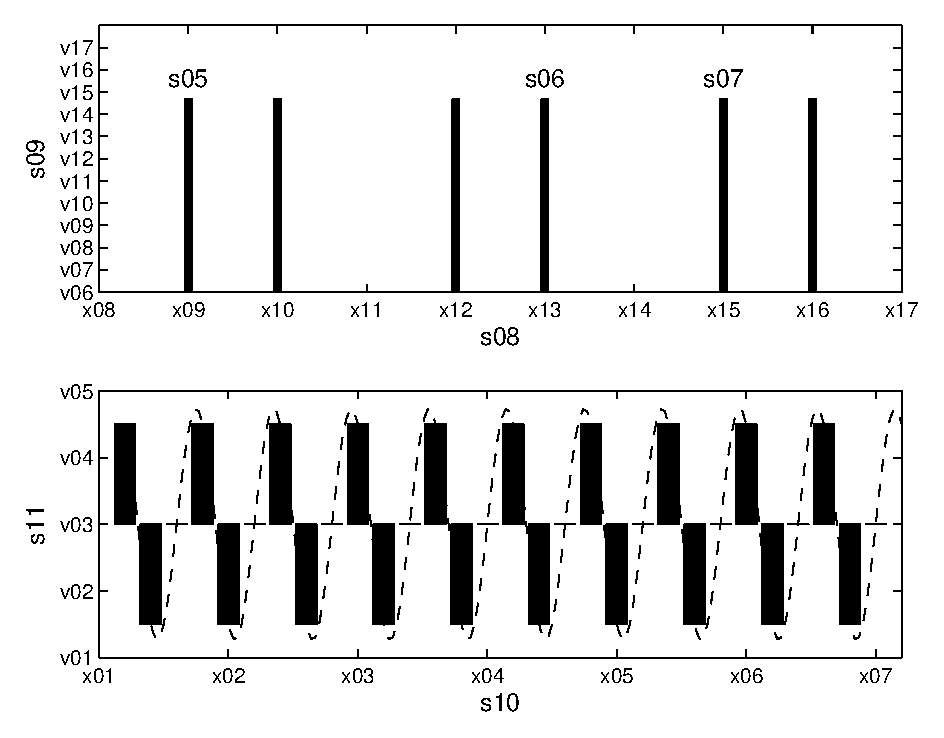
\includegraphics[width=0.47\textwidth]{figs/f_Qs_30_p_10_2.eps}
\end{psfrags}%
%
% End f_Qs_30_p_10_2.tex
\end{document}
% See http://www.mathworks.de/matlabcentral/fileexchange/loadFile.do?objectId=4638
% for recent versions of laprint.m.
%
% created by:           LaPrint version 3.16 (13.9.2004)
% created on:           12-Nov-2008 21:54:09
% eps bounding box:     17.5 cm x 13.125 cm
% comment:              
%
\begin{psfrags}%
\psfragscanon%
%
% text strings:
\psfrag{s05}[b][b]{$\xi_{10}$}
\psfrag{s06}[b][b]{$\xi_{50}$}
\psfrag{s07}[b][b]{$\xi_{70}$}
\psfrag{s08}[t][t]{$\nu$}
\psfrag{s09}[b][b]{$\xi_{\nu}$}
\psfrag{s10}[t][t]{Slot number}
\psfrag{s11}[b][b]{$F_{slot}/\SI{}{A}$}
%
% xticklabels:
\psfrag{x01}[t][t]{0}
\psfrag{x02}[t][t]{5}
\psfrag{x03}[t][t]{10}
\psfrag{x04}[t][t]{15}
\psfrag{x05}[t][t]{20}
\psfrag{x06}[t][t]{25}
\psfrag{x07}[t][t]{30}
\psfrag{x08}[t][t]{0}
\psfrag{x09}[t][t]{10}
\psfrag{x10}[t][t]{20}
\psfrag{x11}[t][t]{30}
\psfrag{x12}[t][t]{40}
\psfrag{x13}[t][t]{50}
\psfrag{x14}[t][t]{60}
\psfrag{x15}[t][t]{70}
\psfrag{x16}[t][t]{80}
\psfrag{x17}[t][t]{90}
%
% yticklabels:
\psfrag{v01}[r][r]{-2}
\psfrag{v02}[r][r]{-1}
\psfrag{v03}[r][r]{0}
\psfrag{v04}[r][r]{1}
\psfrag{v05}[r][r]{2}
\psfrag{v06}[r][r]{0}
\psfrag{v07}[r][r]{0.1}
\psfrag{v08}[r][r]{0.2}
\psfrag{v09}[r][r]{0.3}
\psfrag{v10}[r][r]{0.4}
\psfrag{v11}[r][r]{0.5}
\psfrag{v12}[r][r]{0.6}
\psfrag{v13}[r][r]{0.7}
\psfrag{v14}[r][r]{0.8}
\psfrag{v15}[r][r]{0.9}
\psfrag{v16}[r][r]{1}
\psfrag{v17}[r][r]{1.1}
%
% Figure:
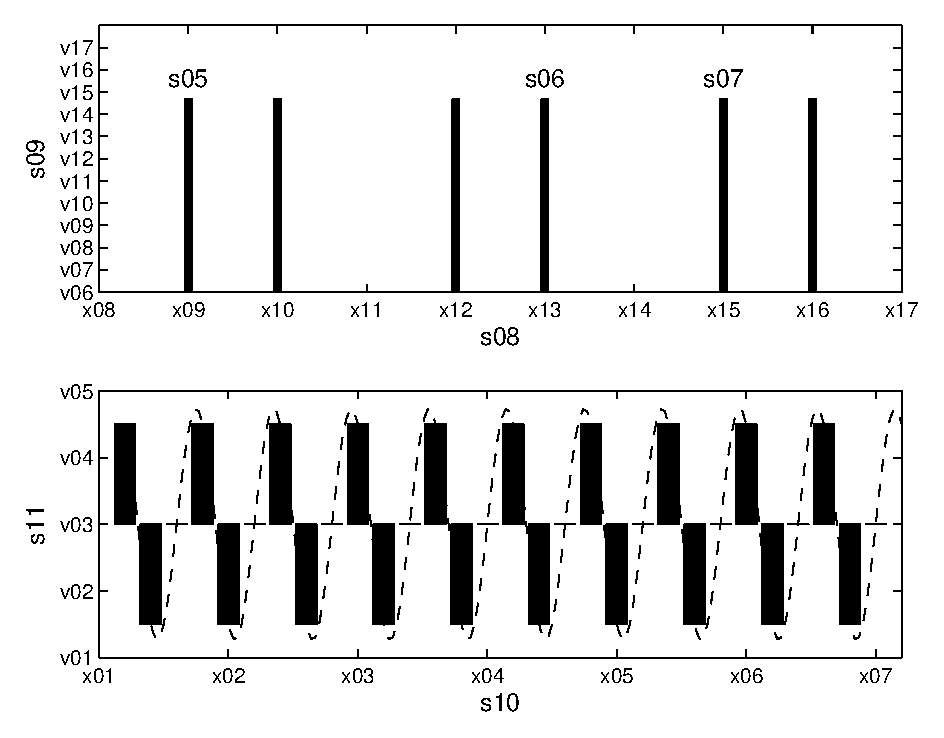
\includegraphics[width=0.47\textwidth]{figs/f_Qs_30_p_10_2.eps}
\end{psfrags}%
%
% End f_Qs_30_p_10_2.tex
}
  \caption{Non-overlapping double layer winding}
  \label{fig:Main_non-overlapping_double}
\end{figure}

\subsubsection{Single layer overlapping}
A general single layer overlapping winding is shown in~% 
Fig.~\ref{fig:Main_single_overlapping}\subref{fig:slw_yd_eq_1}. In this example the coil pitch equals 5. The ingoing coil side of the first coil is in slot 1 and the outgoing coil side in slot 6. It is clear from the figure that the coils overlap. 

The example to illustrate the slot mmf and current sheet has 30 slots and a pole pair number equal to 5. In Tab.~\ref{tab:Example_table} the average pole pitch equals the pole pitch. Therefore this is called a concentrated winding as determined from Fig.~\ref{fig:classification}. The basic winding matrix elements are given as
\begin{equation}
  \mathbf{M_{1,b}} = 
  \begin{pmatrix}
  1&0&0&-1&0&0\\    
  0&-1&0&0&1&0\\   
  0&0&1&0&0&-1\\   
  \end{pmatrix} \
  \mathbf{M_{2,b}} = 
  \begin{pmatrix}
  1& 0&0&-1&0&0\\
  0&-1&0& 0&1&0\\
  0& 0&1& 0&0&-1\\  
  \end{pmatrix} 
\end{equation}
The calculated winding factor along with the slot mmf and current sheet are shown in Fig.~\ref{fig:Main_single_overlapping}\subref{fig:f_Qs30_5_1}. It is important to mention that the coil sides are distributed in such a way as to obtain a sinusoidal slot mmf distribution. The number of slots per pole and phase can be increased to obtain a better sinusoidal distribution. In doing so, the harmonic content will become less.
\begin{figure}[htbp]
  \centering
  \fontsize{6}{6}\selectfont
  \subfloat[Single layer overlapping winding layout\label{fig:slw_yd_eq_1}]{%
  \begin{psfrags}%
\psfragscanon

% text strings:
\psfrag{t01}{{\tiny Coil pitch, $y_d$}}
\psfrag{t02}{{\tiny Overhang, $l_o$}}
\psfrag{t05}{{\tiny 1}}
\psfrag{t06}{{\tiny 2}}
\psfrag{t07}{{\tiny 3}}
\psfrag{t08}{{\tiny 4}}
\psfrag{t09}{{\tiny 5}}
\psfrag{t10}{{\tiny 6}}
\psfrag{t11}{{\tiny Direction of coil assignment}}

% Figure:

\subfloat[Single layer overlapping winding layout\label{fig:slw_yd_eq_1}]
  \hfill
  \subfloat[Slot mmf and winding factors\label{fig:f_Qs30_5_1}]{%
  % This file is generated by the MATLAB m-file laprint.m. It can be included
% into LaTeX documents using the packages graphicx, color and psfrag.
% It is accompanied by a postscript file. A sample LaTeX file is:
%    \documentclass{article}\usepackage{graphicx,color,psfrag}
%    \begin{document}% This file is generated by the MATLAB m-file laprint.m. It can be included
% into LaTeX documents using the packages graphicx, color and psfrag.
% It is accompanied by a postscript file. A sample LaTeX file is:
%    \documentclass{article}\usepackage{graphicx,color,psfrag}
%    \begin{document}\input{f_Qs_30_p_5_1}\end{document}
% See http://www.mathworks.de/matlabcentral/fileexchange/loadFile.do?objectId=4638
% for recent versions of laprint.m.
%
% created by:           LaPrint version 3.16 (13.9.2004)
% created on:           12-Nov-2008 21:46:31
% eps bounding box:     17.5 cm x 13.125 cm
% comment:              
%
\begin{psfrags}%
\psfragscanon%
%
% text strings:
\psfrag{s05}[b][b]{$\xi_{5}$}%
\psfrag{s06}[b][b]{$\xi_{25}$}%
\psfrag{s07}[b][b]{$\xi_{35}$}%
\psfrag{s08}[t][t]{$\nu$}%
\psfrag{s09}[b][b]{$\xi_{\nu}$}%
\psfrag{s10}[t][t]{Slot number}%
\psfrag{s11}[b][b]{$F_{slot}/\SI{}{A}$}%
%
% xticklabels:
\psfrag{x01}[t][t]{0}%
\psfrag{x02}[t][t]{5}%
\psfrag{x03}[t][t]{10}%
\psfrag{x04}[t][t]{15}%
\psfrag{x05}[t][t]{20}%
\psfrag{x06}[t][t]{25}%
\psfrag{x07}[t][t]{30}%
\psfrag{x08}[t][t]{0}%
\psfrag{x09}[t][t]{10}%
\psfrag{x10}[t][t]{20}%
\psfrag{x11}[t][t]{30}%
\psfrag{x12}[t][t]{40}%
\psfrag{x13}[t][t]{50}%
\psfrag{x14}[t][t]{60}%
%
% yticklabels:
\psfrag{v01}[r][r]{-1}%
\psfrag{v02}[r][r]{-0.5}%
\psfrag{v03}[r][r]{0}%
\psfrag{v04}[r][r]{0.5}%
\psfrag{v05}[r][r]{1}%
\psfrag{v06}[r][r]{0}%
\psfrag{v07}[r][r]{0.1}%
\psfrag{v08}[r][r]{0.2}%
\psfrag{v09}[r][r]{0.3}%
\psfrag{v10}[r][r]{0.4}%
\psfrag{v11}[r][r]{0.5}%
\psfrag{v12}[r][r]{0.6}%
\psfrag{v13}[r][r]{0.7}%
\psfrag{v14}[r][r]{0.8}%
\psfrag{v15}[r][r]{0.9}%
\psfrag{v16}[r][r]{1}%
\psfrag{v17}[r][r]{1.1}%
%
% Figure:

\subfloat[Slot mmf and winding factors\label{fig:f_Qs30_5_1}]{%
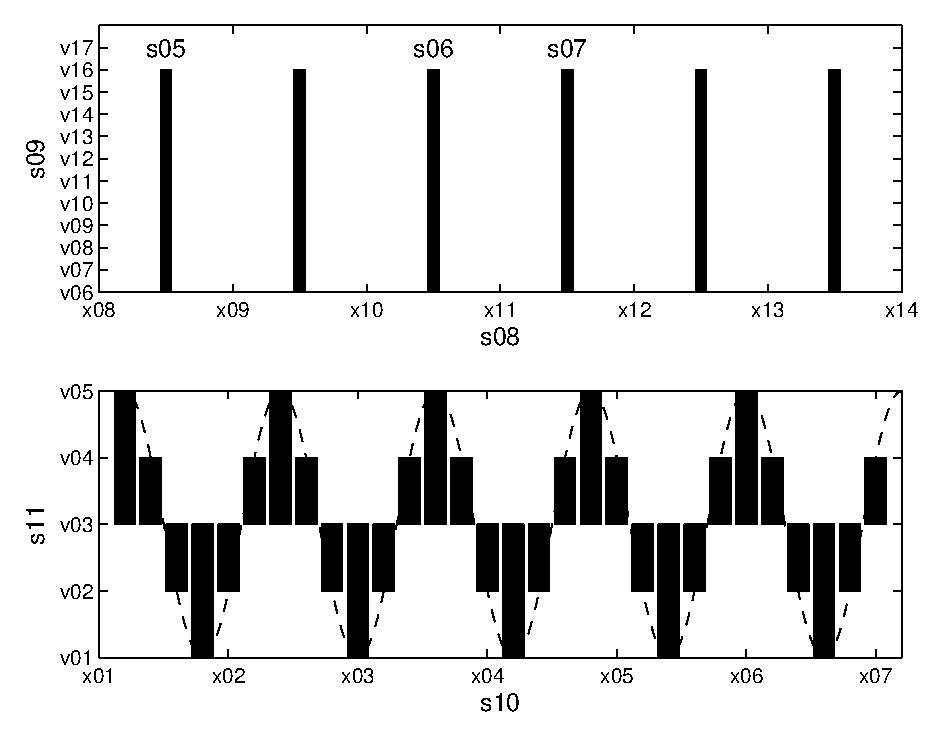
\includegraphics[width=0.9\textwidth]{figs/f_Qs_30_p_5_1.eps}}%
\end{psfrags}%
%
% End f_Qs_30_p_5_1.tex
\end{document}
% See http://www.mathworks.de/matlabcentral/fileexchange/loadFile.do?objectId=4638
% for recent versions of laprint.m.
%
% created by:           LaPrint version 3.16 (13.9.2004)
% created on:           12-Nov-2008 21:46:31
% eps bounding box:     17.5 cm x 13.125 cm
% comment:              
%
\begin{psfrags}%
\psfragscanon%
%
% text strings:
\psfrag{s05}[b][b]{$\xi_{5}$}%
\psfrag{s06}[b][b]{$\xi_{25}$}%
\psfrag{s07}[b][b]{$\xi_{35}$}%
\psfrag{s08}[t][t]{$\nu$}%
\psfrag{s09}[b][b]{$\xi_{\nu}$}%
\psfrag{s10}[t][t]{Slot number}%
\psfrag{s11}[b][b]{$F_{slot}/\SI{}{A}$}%
%
% xticklabels:
\psfrag{x01}[t][t]{0}%
\psfrag{x02}[t][t]{5}%
\psfrag{x03}[t][t]{10}%
\psfrag{x04}[t][t]{15}%
\psfrag{x05}[t][t]{20}%
\psfrag{x06}[t][t]{25}%
\psfrag{x07}[t][t]{30}%
\psfrag{x08}[t][t]{0}%
\psfrag{x09}[t][t]{10}%
\psfrag{x10}[t][t]{20}%
\psfrag{x11}[t][t]{30}%
\psfrag{x12}[t][t]{40}%
\psfrag{x13}[t][t]{50}%
\psfrag{x14}[t][t]{60}%
%
% yticklabels:
\psfrag{v01}[r][r]{-1}%
\psfrag{v02}[r][r]{-0.5}%
\psfrag{v03}[r][r]{0}%
\psfrag{v04}[r][r]{0.5}%
\psfrag{v05}[r][r]{1}%
\psfrag{v06}[r][r]{0}%
\psfrag{v07}[r][r]{0.1}%
\psfrag{v08}[r][r]{0.2}%
\psfrag{v09}[r][r]{0.3}%
\psfrag{v10}[r][r]{0.4}%
\psfrag{v11}[r][r]{0.5}%
\psfrag{v12}[r][r]{0.6}%
\psfrag{v13}[r][r]{0.7}%
\psfrag{v14}[r][r]{0.8}%
\psfrag{v15}[r][r]{0.9}%
\psfrag{v16}[r][r]{1}%
\psfrag{v17}[r][r]{1.1}%
%
% Figure:

\subfloat[Slot mmf and winding factors\label{fig:f_Qs30_5_1}]{%
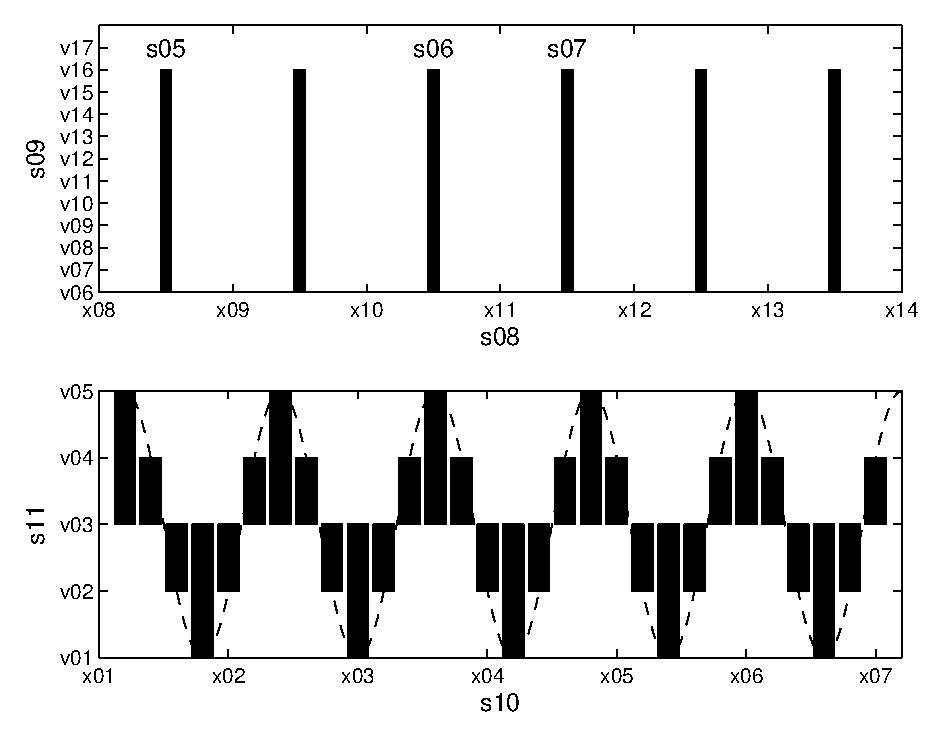
\includegraphics[width=0.9\textwidth]{figs/f_Qs_30_p_5_1.eps}}%
\end{psfrags}%
%
% End f_Qs_30_p_5_1.tex
}
  \caption{Single layer overlapping winding}
  \label{fig:Main_single_overlapping}
\end{figure}

\subsubsection{Double layer overlapping}
A double layer overlapping winding is commonly used in industrial machines. Overlapping double layer windings have a coil pitch greater than one, i.e.~$y_d>1$. Fig.~\ref{fig:dlw_yd_gt_1} shows a double layer winding. Starting at the first slot, the coils are inserted in a counter-clockwise direction. The first coil has its ingoing coil side in the bottom part of slot 1 and the return coil side is in the top part of slot 6. The phase belt constraint in \eqref{eqn:phase_belt_constraint} is used to determine the phase of the coil side in the bottom part of the slot while the top coil sides are given by the coil pitch $y_d$.

Fig.~\ref{fig:f_Qs30_p5_2} shows the slot mmf of a stator with $Q_s=30$ slots and $p=5$ pole pairs. Using the winding properties for this combination given in Tab.~\ref{tab:Example_table}, it is a concentrated winding. The winding has no sub-harmonics. 
\begin{figure}[htbp]
  \centering
  \fontsize{6}{6}\selectfont
  \subfloat[Double layer overlapping winding layout\label{fig:dlw_yd_gt_1}]{%
  \begin{psfrags}%
\psfragscanon

% text strings:
\psfrag{t01}{{\tiny Coil pitch, $y_d$}}
\psfrag{t02}{{\tiny Overhang, $l_o$}}
\psfrag{t03}{{\tiny Top}}
\psfrag{t04}{{\tiny Bottom}}
\psfrag{t05}{{\tiny 1}}
\psfrag{t06}{{\tiny 2}}
\psfrag{t07}{{\tiny 3}}
\psfrag{t08}{{\tiny 4}}
\psfrag{t09}{{\tiny 5}}
\psfrag{t10}{{\tiny 6}}
\psfrag{t11}{{\tiny Direction of coil assignment}}


% Figure:

\subfloat[Double layer overlapping winding layout\label{fig:dlw_yd_gt_1}]
  \hfill
  \subfloat[Slot mmf and winding factors\label{fig:f_Qs30_p5_2}]{%
  % This file is generated by the MATLAB m-file laprint.m. It can be included
% into LaTeX documents using the packages graphicx, color and psfrag.
% It is accompanied by a postscript file. A sample LaTeX file is:
%    \documentclass{article}\usepackage{graphicx,color,psfrag}
%    \begin{document}% This file is generated by the MATLAB m-file laprint.m. It can be included
% into LaTeX documents using the packages graphicx, color and psfrag.
% It is accompanied by a postscript file. A sample LaTeX file is:
%    \documentclass{article}\usepackage{graphicx,color,psfrag}
%    \begin{document}\input{f_Qs_30_p_5_2}\end{document}
% See http://www.mathworks.de/matlabcentral/fileexchange/loadFile.do?objectId=4638
% for recent versions of laprint.m.
%
% created by:           LaPrint version 3.16 (13.9.2004)
% created on:           12-Nov-2008 21:50:28
% eps bounding box:     17.5 cm x 13.125 cm
% comment:              
%
\begin{psfrags}%
\psfragscanon%
%
% text strings:
\psfrag{s05}[b][b]{{\tiny $\xi_{5}$}}%
\psfrag{s06}[b][b]{{\tiny $\xi_{25}$}}%
\psfrag{s07}[b][b]{{\tiny $\xi_{35}$}}%
\psfrag{s08}[t][t]{{\tiny $\nu$}}%
\psfrag{s09}[b][b]{{\tiny $\xi_{\nu}$}}%
\psfrag{s10}[t][t]{{\tiny Slot number}}%
\psfrag{s11}[b][b]{{\tiny $F_{slot}/\SI{}{A}$}}%
%
% xticklabels:
\psfrag{x01}[t][t]{{\tiny 0}}%
\psfrag{x02}[t][t]{{\tiny 5}}%
\psfrag{x03}[t][t]{{\tiny 10}}%
\psfrag{x04}[t][t]{{\tiny 15}}%
\psfrag{x05}[t][t]{{\tiny 20}}%
\psfrag{x06}[t][t]{{\tiny 25}}%
\psfrag{x07}[t][t]{{\tiny 30}}%
\psfrag{x08}[t][t]{{\tiny 0}}%
\psfrag{x09}[t][t]{{\tiny 10}}%
\psfrag{x10}[t][t]{{\tiny 20}}%
\psfrag{x11}[t][t]{{\tiny 30}}%
\psfrag{x12}[t][t]{{\tiny 40}}%
\psfrag{x13}[t][t]{{\tiny 50}}%
\psfrag{x14}[t][t]{{\tiny 60}}%
%
% yticklabels:
\psfrag{v01}[r][r]{{\tiny -2}}%
\psfrag{v02}[r][r]{{\tiny -1}}%
\psfrag{v03}[r][r]{{\tiny 0}}%
\psfrag{v04}[r][r]{{\tiny 1}}%
\psfrag{v05}[r][r]{{\tiny 2}}%
\psfrag{v06}[r][r]{{\tiny 0}}%
\psfrag{v07}[r][r]{{\tiny 0.1}}%
\psfrag{v08}[r][r]{{\tiny 0.2}}%
\psfrag{v09}[r][r]{{\tiny 0.3}}%
\psfrag{v10}[r][r]{{\tiny 0.4}}%
\psfrag{v11}[r][r]{{\tiny 0.5}}%
\psfrag{v12}[r][r]{{\tiny 0.6}}%
\psfrag{v13}[r][r]{{\tiny 0.7}}%
\psfrag{v14}[r][r]{{\tiny 0.8}}%
\psfrag{v15}[r][r]{{\tiny 0.9}}%
\psfrag{v16}[r][r]{{\tiny 1}}%
\psfrag{v17}[r][r]{{\tiny 1.1}}%
%
% Figure:

\subfloat[Slot mmf and winding factors\label{fig:f_Qs30_p5_2}]{%
\includegraphics[width=0.9\textwidth]{figs/f_Qs_30_p_5_2.eps}}%
\end{psfrags}%
%
% End f_Qs_30_p_5_2.tex
\end{document}
% See http://www.mathworks.de/matlabcentral/fileexchange/loadFile.do?objectId=4638
% for recent versions of laprint.m.
%
% created by:           LaPrint version 3.16 (13.9.2004)
% created on:           12-Nov-2008 21:50:28
% eps bounding box:     17.5 cm x 13.125 cm
% comment:              
%
\begin{psfrags}%
\psfragscanon%
%
% text strings:
\psfrag{s05}[b][b]{{\tiny $\xi_{5}$}}%
\psfrag{s06}[b][b]{{\tiny $\xi_{25}$}}%
\psfrag{s07}[b][b]{{\tiny $\xi_{35}$}}%
\psfrag{s08}[t][t]{{\tiny $\nu$}}%
\psfrag{s09}[b][b]{{\tiny $\xi_{\nu}$}}%
\psfrag{s10}[t][t]{{\tiny Slot number}}%
\psfrag{s11}[b][b]{{\tiny $F_{slot}/\SI{}{A}$}}%
%
% xticklabels:
\psfrag{x01}[t][t]{{\tiny 0}}%
\psfrag{x02}[t][t]{{\tiny 5}}%
\psfrag{x03}[t][t]{{\tiny 10}}%
\psfrag{x04}[t][t]{{\tiny 15}}%
\psfrag{x05}[t][t]{{\tiny 20}}%
\psfrag{x06}[t][t]{{\tiny 25}}%
\psfrag{x07}[t][t]{{\tiny 30}}%
\psfrag{x08}[t][t]{{\tiny 0}}%
\psfrag{x09}[t][t]{{\tiny 10}}%
\psfrag{x10}[t][t]{{\tiny 20}}%
\psfrag{x11}[t][t]{{\tiny 30}}%
\psfrag{x12}[t][t]{{\tiny 40}}%
\psfrag{x13}[t][t]{{\tiny 50}}%
\psfrag{x14}[t][t]{{\tiny 60}}%
%
% yticklabels:
\psfrag{v01}[r][r]{{\tiny -2}}%
\psfrag{v02}[r][r]{{\tiny -1}}%
\psfrag{v03}[r][r]{{\tiny 0}}%
\psfrag{v04}[r][r]{{\tiny 1}}%
\psfrag{v05}[r][r]{{\tiny 2}}%
\psfrag{v06}[r][r]{{\tiny 0}}%
\psfrag{v07}[r][r]{{\tiny 0.1}}%
\psfrag{v08}[r][r]{{\tiny 0.2}}%
\psfrag{v09}[r][r]{{\tiny 0.3}}%
\psfrag{v10}[r][r]{{\tiny 0.4}}%
\psfrag{v11}[r][r]{{\tiny 0.5}}%
\psfrag{v12}[r][r]{{\tiny 0.6}}%
\psfrag{v13}[r][r]{{\tiny 0.7}}%
\psfrag{v14}[r][r]{{\tiny 0.8}}%
\psfrag{v15}[r][r]{{\tiny 0.9}}%
\psfrag{v16}[r][r]{{\tiny 1}}%
\psfrag{v17}[r][r]{{\tiny 1.1}}%
%
% Figure:

\subfloat[Slot mmf and winding factors\label{fig:f_Qs30_p5_2}]{%
\includegraphics[width=0.9\textwidth]{figs/f_Qs_30_p_5_2.eps}}%
\end{psfrags}%
%
% End f_Qs_30_p_5_2.tex
}
  \caption{Double layer overlapping winding}
  \label{Main_double_overlapping}
\end{figure}

\clearpage
\section{Summary}
In this report an algorithm was derived to present a winding in a matrix form. This compact form allows the calculation of the winding factors for all harmonics. The basis of the algorithm is the phase belt sequence and the phase belt constraint which are derived from the air gap mmf envelope functions. 

\begin{figure}[htbp]
  \centering
  \fontsize{8}{6}\selectfont
  \begin{overpic}[scale=1.5,grid]
  {figs/f_double_layer_ex}
  \put(6.3,7.2){+1}  
  \put(6.3,10.8){+1}
  \put(16,7.2){-2}
  \put(16,10.8){-2}
  \put(25.6,7.2){+3}
  \put(25.6,10.8){+3}
  \put(35.2,7.2){-1}  
  \put(35.2,10.8){-1}
  \put(44.5,7.2){+2}
  \put(44.5,10.8){+2}
  \put(54.1,7.2){-3}
  \put(54.1,10.8){-3}
  \put(6.5,3){$\tau_s=\SI{12}{\arcdeg}$}
  \put(6.5,17){$\SI{0}{\arcdeg}$}  
  \dashline{1}(7,20)(7.5,78)
  \put(19.8,17){$\SI{18}{\arcdeg}$}  
  \dashline{1}(21,20)(21,78)
  \end{overpic}
  \caption{Double layer overlapping winding}
  \label{Main_double_overlapping}
\end{figure}

\begin{appendices}

\chapter{Discrete Fourier Transform}
In this report it is assumed that the harmonic order of the spatial signal is known. The DFT is primarily used to identify the amplitude of the harmonics. Furthermore, the considered function is periodic: $f(x_1)=f(x_{N+1})$.

The base function used in the analysis is the $\cos(\theta-\phi)$ function, where $\phi$ is the phase shift. The visualisation for different values of phase shift is shown in Fig.~\ref{fig:base}.  

\begin{figure}[htbp]
  \centering
  \fontsize{6}{0}\selectfont
  \setlength\fwidth{0.26\textwidth}
  \subfloat[$\cos\bigl(\theta-(-30)\bigr)$]{
  % This file was created by matlab2tikz.
%
%The latest updates can be retrieved from
%  http://www.mathworks.com/matlabcentral/fileexchange/22022-matlab2tikz-matlab2tikz
%where you can also make suggestions and rate matlab2tikz.
%
\begin{tikzpicture}

\begin{axis}[%
width=0.951\fwidth,
height=0.75\fwidth,
at={(0\fwidth,0\fwidth)},
scale only axis,
xmin=-180,
xmax=180,
xtick={-180,    0,  180},
xlabel={$\theta/\SI{}{\arcdeg}$},
xmajorgrids,
ymin=-0.999874127673875,
ymax=0.999874127673875,
ylabel={$\cos(\theta-\phi)$},
ymajorgrids,
axis background/.style={fill=white},
legend style={legend cell align=left,align=left,legend plot pos=left,draw=black}
]
\addplot [color=black,solid]
  table[row sep=crcr]{%
-180	-0.866025403784439\\
-176.363636363636	-0.832569854634771\\
-172.727272727273	-0.795761840530832\\
-169.090909090909	-0.755749574354258\\
-165.454545454545	-0.712694171378863\\
-161.818181818182	-0.666769000516292\\
-158.181818181818	-0.618158986220605\\
-154.545454545455	-0.567059863862771\\
-150.909090909091	-0.513677391573407\\
-147.272727272727	-0.45822652172741\\
-143.636363636364	-0.400930535406614\\
-140	-0.342020143325669\\
-136.363636363636	-0.28173255684143\\
-132.727272727273	-0.220310532786541\\
-129.090909090909	-0.15800139597335\\
-125.454545454545	-0.0950560433041827\\
-121.818181818182	-0.0317279334980679\\
-118.181818181818	0.0317279334980676\\
-114.545454545455	0.0950560433041828\\
-110.909090909091	0.15800139597335\\
-107.272727272727	0.220310532786541\\
-103.636363636364	0.28173255684143\\
-100	0.342020143325669\\
-96.3636363636364	0.400930535406614\\
-92.7272727272727	0.45822652172741\\
-89.0909090909091	0.513677391573407\\
-85.4545454545455	0.567059863862771\\
-81.8181818181818	0.618158986220605\\
-78.1818181818182	0.666769000516292\\
-74.5454545454545	0.712694171378863\\
-70.9090909090909	0.755749574354258\\
-67.2727272727273	0.795761840530832\\
-63.6363636363636	0.832569854634771\\
-60	0.866025403784439\\
-56.3636363636364	0.895993774291336\\
-52.7272727272727	0.922354294104581\\
-49.0909090909091	0.945000818714668\\
-45.4545454545454	0.963842158559942\\
-41.8181818181818	0.978802446214779\\
-38.1818181818182	0.989821441880933\\
-34.5454545454545	0.996854775951942\\
-30.9090909090909	0.999874127673875\\
-27.2727272727273	0.998867339183008\\
-23.6363636363636	0.993838464461254\\
-20	0.984807753012208\\
-16.3636363636364	0.971811568323542\\
-12.7272727272727	0.954902241444074\\
-9.09090909090908	0.934147860265107\\
-5.45454545454543	0.909631995354518\\
-1.81818181818181	0.881453363447582\\
1.81818181818184	0.849725429949514\\
5.45454545454546	0.814575952050336\\
9.09090909090911	0.776146464291757\\
12.7272727272727	0.734591708657533\\
16.3636363636364	0.690079011482112\\
20	0.642787609686539\\
23.6363636363637	0.59290792905464\\
27.2727272727273	0.540640817455598\\
30.9090909090909	0.486196736100469\\
34.5454545454545	0.429794912089172\\
38.1818181818182	0.371662455660328\\
41.8181818181818	0.312033445698487\\
45.4545454545455	0.251147987181079\\
49.0909090909091	0.18925124436041\\
52.7272727272727	0.126592453573749\\
56.3636363636364	0.0634239196565648\\
60	-3.82858892158944e-016\\
63.6363636363637	-0.0634239196565647\\
67.2727272727273	-0.126592453573749\\
70.9090909090909	-0.18925124436041\\
74.5454545454546	-0.25114798718108\\
78.1818181818182	-0.312033445698487\\
81.8181818181818	-0.371662455660327\\
85.4545454545455	-0.429794912089171\\
89.0909090909091	-0.486196736100469\\
92.7272727272727	-0.540640817455598\\
96.3636363636364	-0.59290792905464\\
100	-0.642787609686539\\
103.636363636364	-0.690079011482112\\
107.272727272727	-0.734591708657533\\
110.909090909091	-0.776146464291757\\
114.545454545455	-0.814575952050336\\
118.181818181818	-0.849725429949514\\
121.818181818182	-0.881453363447582\\
125.454545454545	-0.909631995354518\\
129.090909090909	-0.934147860265107\\
132.727272727273	-0.954902241444074\\
136.363636363636	-0.971811568323542\\
140	-0.984807753012208\\
143.636363636364	-0.993838464461254\\
147.272727272727	-0.998867339183008\\
150.909090909091	-0.999874127673875\\
154.545454545455	-0.996854775951942\\
158.181818181818	-0.989821441880933\\
161.818181818182	-0.978802446214779\\
165.454545454545	-0.963842158559942\\
169.090909090909	-0.945000818714668\\
172.727272727273	-0.922354294104581\\
176.363636363636	-0.895993774291336\\
180	-0.866025403784439\\
};

\addplot [color=blue,only marks,mark=o,mark options={solid}]
  table[row sep=crcr]{%
-180	-0.866025403784439\\
-152.307692307692	-0.534465805383544\\
-124.615384615385	-0.080466567836728\\
-96.9230769230769	0.391966606025713\\
-69.2307692307692	0.774604929331893\\
-41.5384615384616	0.979790648616705\\
-13.8461538461539	0.960518081924436\\
13.8461538461538	0.721202425731447\\
41.5384615384615	0.316667992325635\\
69.2307692307692	-0.160411274341826\\
96.9230769230769	-0.600742256776532\\
124.615384615385	-0.903450415706285\\
152.307692307692	-0.999188960281069\\
180	-0.866025403784439\\
};

\addplot [color=red,dashed]
  table[row sep=crcr]{%
-180	-0.866025384341204\\
-176.363636363636	-0.832569835950002\\
-172.727272727273	-0.795761822679717\\
-169.090909090909	-0.755749557408629\\
-165.454545454545	-0.712694155406906\\
-161.818181818182	-0.666768985582272\\
-158.181818181818	-0.61815897238461\\
-154.545454545455	-0.567059851180464\\
-150.909090909091	-0.513677380095808\\
-147.272727272727	-0.458226511500688\\
-143.636363636364	-0.4009305264719\\
-140	-0.342020135718892\\
-136.363636363636	-0.281732550593172\\
-132.727272727273	-0.220310527921913\\
-129.090909090909	-0.158001392511893\\
-125.454545454545	-0.0950560412597869\\
-121.818181818182	-0.0317279328789172\\
-118.181818181818	0.0317279326895279\\
-114.545454545455	0.0950560410712561\\
-110.909090909091	0.158001392325076\\
-107.272727272727	0.220310527737657\\
-103.636363636364	0.281732550412314\\
-100	0.342020135542257\\
-96.3636363636364	0.400930526300295\\
-92.7272727272727	0.458226511334901\\
-89.0909090909091	0.513677379936601\\
-85.4545454545455	0.567059851028574\\
-81.8181818181818	0.618158972240744\\
-78.1818181818182	0.666768985447106\\
-74.5454545454545	0.712694155281079\\
-70.9090909090909	0.755749557292744\\
-67.2727272727273	0.795761822574336\\
-63.6363636363636	0.832569835855645\\
-60	0.866025384258348\\
-56.3636363636364	0.895993754096953\\
-52.7272727272727	0.92235427332327\\
-49.0909090909091	0.945000797430155\\
-45.4545454545454	0.96384213685798\\
-41.8181818181818	0.978802424182802\\
-38.1818181818182	0.989821419607705\\
-34.5454545454545	0.996854753527197\\
-30.9090909090909	0.999874105187957\\
-27.2727272727273	0.998867316726507\\
-23.6363636363636	0.993838442124644\\
-20	0.984807730885477\\
-16.3636363636364	0.971811546495835\\
-12.7272727272727	0.954902220003331\\
-9.09090909090908	0.934147839297711\\
-5.45454545454543	0.909631974944945\\
-1.81818181818181	0.881453343678061\\
1.81818181818184	0.849725410899699\\
5.45454545454546	0.814575933796981\\
9.09090909090911	0.77614644690841\\
12.7272727272727	0.734591692214239\\
16.3636363636364	0.690078996045129\\
20	0.642787595318076\\
23.6363636363637	0.5929079158126\\
27.2727272727273	0.54064080539335\\
30.9090909090909	0.486196725266632\\
34.5454545454545	0.429794902527417\\
38.1818181818182	0.371662447409205\\
41.8181818181818	0.31203343879127\\
45.4545454545455	0.251147981645627\\
49.0909090909091	0.189251240219061\\
52.7272727272727	0.126592450843226\\
56.3636363636364	0.0634239183479103\\
60	1.18531457202731e-010\\
63.6363636363637	-0.0634239181112759\\
67.2727272727273	-0.126592450607878\\
70.9090909090909	-0.189251239985851\\
74.5454545454546	-0.2511479814154\\
78.1818181818182	-0.312033438564855\\
81.8181818181818	-0.371662447187419\\
85.4545454545455	-0.429794902311057\\
89.0909090909091	-0.486196725056474\\
92.7272727272727	-0.540640805190144\\
96.3636363636364	-0.592907915617068\\
100	-0.64278759513091\\
103.636363636364	-0.690078995866988\\
107.272727272727	-0.734591692045743\\
110.909090909091	-0.776146446750142\\
114.545454545455	-0.814575933649483\\
118.181818181818	-0.849725410763469\\
121.818181818182	-0.881453343553552\\
125.454545454545	-0.909631974832562\\
129.090909090909	-0.93414783919781\\
132.727272727273	-0.95490221991622\\
136.363636363636	-0.971811546421768\\
140	-0.984807730824658\\
143.636363636364	-0.99383844207722\\
147.272727272727	-0.998867316692575\\
150.909090909091	-0.999874105167557\\
154.545454545455	-0.996854753520316\\
158.181818181818	-0.989821419614274\\
161.818181818182	-0.9788024242027\\
165.454545454545	-0.96384213689103\\
169.090909090909	-0.945000797476129\\
172.727272727273	-0.922354273381886\\
176.363636363636	-0.89599375416788\\
180	-0.866025384341205\\
};

\node[right, align=left, text=black]
at (axis cs:-135,-0.7) {input: $\phi = \SI{-30}{\arcdeg}$};
\node[right, align=left, text=black]
at (axis cs:-135,-0.9) {result: $\phi = \SI{-30}{\arcdeg}$};
\end{axis}
\end{tikzpicture}%}
  \hfill
  \subfloat[$\cos(\theta)$]{
  % This file was created by matlab2tikz.
%
%The latest updates can be retrieved from
%  http://www.mathworks.com/matlabcentral/fileexchange/22022-matlab2tikz-matlab2tikz
%where you can also make suggestions and rate matlab2tikz.
%
\begin{tikzpicture}

\begin{axis}[%
width=0.951\fwidth,
height=0.75\fwidth,
at={(0\fwidth,0\fwidth)},
scale only axis,
xmin=-180,
xmax=180,
xtick={-180,    0,  180},
xlabel={$\theta/\SI{}{\arcdeg}$},
xmajorgrids,
ymin=-1,
ymax=0.999496542383185,
ylabel={$\cos(\theta-\phi)$},
ymajorgrids,
axis background/.style={fill=white},
legend style={legend cell align=left,align=left,legend plot pos=left,draw=black}
]
\addplot [color=black,solid]
  table[row sep=crcr]{%
-180	-1\\
-176.363636363636	-0.997986676471884\\
-172.727272727273	-0.991954812830795\\
-169.090909090909	-0.981928697262707\\
-165.454545454545	-0.967948701396356\\
-161.818181818182	-0.950071117740945\\
-158.181818181818	-0.928367933016073\\
-154.545454545455	-0.902926538286621\\
-150.909090909091	-0.873849377069785\\
-147.272727272727	-0.841253532831181\\
-143.636363636364	-0.805270257531059\\
-140	-0.766044443118978\\
-136.363636363636	-0.72373403810507\\
-132.727272727273	-0.678509411557132\\
-129.090909090909	-0.630552667084522\\
-125.454545454545	-0.580056909571198\\
-121.818181818182	-0.527225467610502\\
-118.181818181818	-0.472271074772683\\
-114.545454545455	-0.415415013001886\\
-110.909090909091	-0.356886221591872\\
-107.272727272727	-0.296920375328275\\
-103.636363636364	-0.235758935509427\\
-100	-0.17364817766693\\
-96.3636363636364	-0.110838199901011\\
-92.7272727272727	-0.0475819158237421\\
-89.0909090909091	0.0158659638348082\\
-85.4545454545455	0.0792499568567887\\
-81.8181818181818	0.142314838273285\\
-78.1818181818182	0.204806668065191\\
-74.5454545454545	0.266473813690035\\
-70.9090909090909	0.327067963317422\\
-67.2727272727273	0.386345125693129\\
-63.6363636363636	0.444066612605774\\
-60	0.5\\
-56.3636363636364	0.55392006386611\\
-52.7272727272727	0.605609687137667\\
-49.0909090909091	0.654860733945285\\
-45.4545454545454	0.701474887706321\\
-41.8181818181818	0.745264449675755\\
-38.1818181818182	0.786053094742788\\
-34.5454545454545	0.823676581429833\\
-30.9090909090909	0.857983413234977\\
-27.2727272727273	0.888835448654923\\
-23.6363636363636	0.91610845743207\\
-20	0.939692620785908\\
-16.3636363636364	0.959492973614497\\
-12.7272727272727	0.975429786885407\\
-9.09090909090908	0.987438888676394\\
-5.45454545454543	0.995471922573085\\
-1.81818181818181	0.999496542383185\\
1.81818181818184	0.999496542383185\\
5.45454545454546	0.995471922573085\\
9.09090909090911	0.987438888676394\\
12.7272727272727	0.975429786885407\\
16.3636363636364	0.959492973614497\\
20	0.939692620785908\\
23.6363636363637	0.916108457432069\\
27.2727272727273	0.888835448654923\\
30.9090909090909	0.857983413234977\\
34.5454545454545	0.823676581429833\\
38.1818181818182	0.786053094742787\\
41.8181818181818	0.745264449675755\\
45.4545454545455	0.701474887706321\\
49.0909090909091	0.654860733945285\\
52.7272727272727	0.605609687137667\\
56.3636363636364	0.55392006386611\\
60	0.5\\
63.6363636363637	0.444066612605774\\
67.2727272727273	0.386345125693129\\
70.9090909090909	0.327067963317422\\
74.5454545454546	0.266473813690035\\
78.1818181818182	0.20480666806519\\
81.8181818181818	0.142314838273285\\
85.4545454545455	0.0792499568567887\\
89.0909090909091	0.0158659638348075\\
92.7272727272727	-0.0475819158237425\\
96.3636363636364	-0.110838199901011\\
100	-0.17364817766693\\
103.636363636364	-0.235758935509428\\
107.272727272727	-0.296920375328275\\
110.909090909091	-0.356886221591872\\
114.545454545455	-0.415415013001887\\
118.181818181818	-0.472271074772683\\
121.818181818182	-0.527225467610502\\
125.454545454545	-0.580056909571198\\
129.090909090909	-0.630552667084523\\
132.727272727273	-0.678509411557132\\
136.363636363636	-0.72373403810507\\
140	-0.766044443118978\\
143.636363636364	-0.805270257531059\\
147.272727272727	-0.841253532831181\\
150.909090909091	-0.873849377069785\\
154.545454545455	-0.902926538286621\\
158.181818181818	-0.928367933016073\\
161.818181818182	-0.950071117740945\\
165.454545454545	-0.967948701396356\\
169.090909090909	-0.981928697262707\\
172.727272727273	-0.991954812830795\\
176.363636363636	-0.997986676471884\\
180	-1\\
};

\addplot [color=blue,only marks,mark=o,mark options={solid}]
  table[row sep=crcr]{%
-180	-1\\
-152.307692307692	-0.885455991800417\\
-124.615384615385	-0.568064735308803\\
-96.9230769230769	-0.120536678161225\\
-69.2307692307692	0.354604872043075\\
-41.5384615384616	0.748510745341276\\
-13.8461538461539	0.970941787796838\\
13.8461538461538	0.970941787796839\\
41.5384615384615	0.748510745341276\\
69.2307692307692	0.354604872043075\\
96.9230769230769	-0.120536678161224\\
124.615384615385	-0.568064735308803\\
152.307692307692	-0.885455991800417\\
180	-1\\
};

\addplot [color=red,dashed]
  table[row sep=crcr]{%
-180	-0.999999977548887\\
-176.363636363636	-0.997986654065945\\
-172.727272727273	-0.991954790560195\\
-169.090909090909	-0.981928675217066\\
-165.454545454545	-0.96794867966439\\
-161.818181818182	-0.950071096410106\\
-158.181818181818	-0.928367912172195\\
-154.545454545455	-0.902926518013582\\
-150.909090909091	-0.873849357449161\\
-147.272727272727	-0.841253513941923\\
-143.636363636364	-0.805270239449171\\
-140	-0.766044425917215\\
-136.363636363636	-0.723734021852642\\
-132.727272727273	-0.678509396319426\\
-129.090909090909	-0.63055265292284\\
-125.454545454545	-0.580056896542508\\
-121.818181818182	-0.527225455767212\\
-118.181818181818	-0.472271064162425\\
-114.545454545455	-0.41541500366733\\
-110.909090909091	-0.356886213570548\\
-107.272727272727	-0.296920368652428\\
-103.636363636364	-0.235758930205883\\
-100	-0.173648173756988\\
-96.3636363636364	-0.110838197400361\\
-92.7272727272727	-0.047581914742397\\
-89.0909090909091	0.0158659634925489\\
-85.4545454545455	0.0792499550923586\\
-81.8181818181818	0.142314835093844\\
-78.1818181818182	0.204806663483597\\
-74.5454545454545	0.266473807724792\\
-70.9090909090909	0.327067955992604\\
-67.2727272727273	0.386345117038287\\
-63.6363636363636	0.444066602655814\\
-60	0.499999988795041\\
-56.3636363636364	0.553920051451326\\
-52.7272727272727	0.605609673563103\\
-49.0909090909091	0.654860719265656\\
-45.4545454545454	0.701474871980793\\
-41.8181818181818	0.745264432967703\\
-38.1818181818182	0.786053077119546\\
-34.5454545454545	0.823676562962418\\
-30.9090909090909	0.857983393997807\\
-27.2727272727273	0.888835428725515\\
-23.6363636363636	0.916108436890726\\
-20	0.939692599715398\\
-16.3636363636364	0.959492952099719\\
-12.7272727272727	0.975429765013048\\
-9.09090909090908	0.987438866534583\\
-5.45454545454543	0.995471900251033\\
-1.81818181818181	0.999496519970831\\
1.81818181818184	0.999496519970831\\
5.45454545454546	0.995471900251033\\
9.09090909090911	0.987438866534583\\
12.7272727272727	0.975429765013048\\
16.3636363636364	0.959492952099719\\
20	0.939692599715398\\
23.6363636363637	0.916108436890726\\
27.2727272727273	0.888835428725515\\
30.9090909090909	0.857983393997807\\
34.5454545454545	0.823676562962418\\
38.1818181818182	0.786053077119546\\
41.8181818181818	0.745264432967703\\
45.4545454545455	0.701474871980793\\
49.0909090909091	0.654860719265656\\
52.7272727272727	0.605609673563102\\
56.3636363636364	0.553920051451326\\
60	0.49999998879504\\
63.6363636363637	0.444066602655813\\
67.2727272727273	0.386345117038287\\
70.9090909090909	0.327067955992604\\
74.5454545454546	0.266473807724791\\
78.1818181818182	0.204806663483596\\
81.8181818181818	0.142314835093844\\
85.4545454545455	0.0792499550923586\\
89.0909090909091	0.0158659634925482\\
92.7272727272727	-0.0475819147423975\\
96.3636363636364	-0.110838197400361\\
100	-0.173648173756988\\
103.636363636364	-0.235758930205883\\
107.272727272727	-0.296920368652428\\
110.909090909091	-0.356886213570548\\
114.545454545455	-0.41541500366733\\
118.181818181818	-0.472271064162425\\
121.818181818182	-0.527225455767212\\
125.454545454545	-0.580056896542508\\
129.090909090909	-0.630552652922841\\
132.727272727273	-0.678509396319426\\
136.363636363636	-0.723734021852642\\
140	-0.766044425917215\\
143.636363636364	-0.805270239449171\\
147.272727272727	-0.841253513941923\\
150.909090909091	-0.873849357449161\\
154.545454545455	-0.902926518013582\\
158.181818181818	-0.928367912172196\\
161.818181818182	-0.950071096410106\\
165.454545454545	-0.96794867966439\\
169.090909090909	-0.981928675217067\\
172.727272727273	-0.991954790560195\\
176.363636363636	-0.997986654065945\\
180	-0.999999977548887\\
};

\node[right, align=left, text=black]
at (axis cs:-135,-0.7) {input: $\phi = \SI{0}{\arcdeg}$};
\node[right, align=left, text=black]
at (axis cs:-135,-0.9) {result: $\phi = \SI{0}{\arcdeg}$};
\end{axis}
\end{tikzpicture}%}
  \hfill
  \subfloat[$\cos\bigl(\theta-(+30)\bigr)$]{
  % This file was created by matlab2tikz.
%
%The latest updates can be retrieved from
%  http://www.mathworks.com/matlabcentral/fileexchange/22022-matlab2tikz-matlab2tikz
%where you can also make suggestions and rate matlab2tikz.
%
\begin{tikzpicture}

\begin{axis}[%
width=0.951\fwidth,
height=0.75\fwidth,
at={(0\fwidth,0\fwidth)},
scale only axis,
xmin=-180,
xmax=180,
xtick={-180,    0,  180},
xlabel={$\theta/\SI{}{\arcdeg}$},
xmajorgrids,
ymin=-0.999874127673875,
ymax=0.999874127673875,
ylabel={$\cos(\theta-\phi)$},
ymajorgrids,
axis background/.style={fill=white},
legend style={legend cell align=left,align=left,legend plot pos=left,draw=black}
]
\addplot [color=black,solid]
  table[row sep=crcr]{%
-180	-0.866025403784439\\
-176.363636363636	-0.895993774291336\\
-172.727272727273	-0.922354294104581\\
-169.090909090909	-0.945000818714669\\
-165.454545454545	-0.963842158559942\\
-161.818181818182	-0.978802446214779\\
-158.181818181818	-0.989821441880933\\
-154.545454545455	-0.996854775951942\\
-150.909090909091	-0.999874127673875\\
-147.272727272727	-0.998867339183008\\
-143.636363636364	-0.993838464461254\\
-140	-0.984807753012208\\
-136.363636363636	-0.971811568323542\\
-132.727272727273	-0.954902241444074\\
-129.090909090909	-0.934147860265107\\
-125.454545454545	-0.909631995354518\\
-121.818181818182	-0.881453363447582\\
-118.181818181818	-0.849725429949514\\
-114.545454545455	-0.814575952050336\\
-110.909090909091	-0.776146464291757\\
-107.272727272727	-0.734591708657533\\
-103.636363636364	-0.690079011482112\\
-100	-0.642787609686539\\
-96.3636363636364	-0.59290792905464\\
-92.7272727272727	-0.540640817455597\\
-89.0909090909091	-0.486196736100469\\
-85.4545454545455	-0.429794912089171\\
-81.8181818181818	-0.371662455660327\\
-78.1818181818182	-0.312033445698487\\
-74.5454545454545	-0.251147987181079\\
-70.9090909090909	-0.18925124436041\\
-67.2727272727273	-0.126592453573749\\
-63.6363636363636	-0.0634239196565642\\
-60	5.05319527541181e-016\\
-56.3636363636364	0.0634239196565648\\
-52.7272727272727	0.12659245357375\\
-49.0909090909091	0.18925124436041\\
-45.4545454545454	0.25114798718108\\
-41.8181818181818	0.312033445698487\\
-38.1818181818182	0.371662455660328\\
-34.5454545454545	0.429794912089172\\
-30.9090909090909	0.486196736100469\\
-27.2727272727273	0.540640817455598\\
-23.6363636363636	0.592907929054641\\
-20	0.642787609686539\\
-16.3636363636364	0.690079011482112\\
-12.7272727272727	0.734591708657533\\
-9.09090909090908	0.776146464291757\\
-5.45454545454543	0.814575952050336\\
-1.81818181818181	0.849725429949514\\
1.81818181818184	0.881453363447582\\
5.45454545454546	0.909631995354518\\
9.09090909090911	0.934147860265107\\
12.7272727272727	0.954902241444074\\
16.3636363636364	0.971811568323542\\
20	0.984807753012208\\
23.6363636363637	0.993838464461254\\
27.2727272727273	0.998867339183008\\
30.9090909090909	0.999874127673875\\
34.5454545454545	0.996854775951942\\
38.1818181818182	0.989821441880933\\
41.8181818181818	0.978802446214779\\
45.4545454545455	0.963842158559942\\
49.0909090909091	0.945000818714668\\
52.7272727272727	0.922354294104581\\
56.3636363636364	0.895993774291336\\
60	0.866025403784438\\
63.6363636363637	0.832569854634771\\
67.2727272727273	0.795761840530832\\
70.9090909090909	0.755749574354258\\
74.5454545454546	0.712694171378862\\
78.1818181818182	0.666769000516291\\
81.8181818181818	0.618158986220605\\
85.4545454545455	0.567059863862771\\
89.0909090909091	0.513677391573406\\
92.7272727272727	0.45822652172741\\
96.3636363636364	0.400930535406614\\
100	0.342020143325669\\
103.636363636364	0.281732556841429\\
107.272727272727	0.22031053278654\\
110.909090909091	0.15800139597335\\
114.545454545455	0.0950560433041819\\
118.181818181818	0.0317279334980671\\
121.818181818182	-0.0317279334980679\\
125.454545454545	-0.0950560433041827\\
129.090909090909	-0.158001395973351\\
132.727272727273	-0.220310532786541\\
136.363636363636	-0.28173255684143\\
140	-0.342020143325669\\
143.636363636364	-0.400930535406614\\
147.272727272727	-0.458226521727411\\
150.909090909091	-0.513677391573407\\
154.545454545455	-0.567059863862771\\
158.181818181818	-0.618158986220606\\
161.818181818182	-0.666769000516292\\
165.454545454545	-0.712694171378863\\
169.090909090909	-0.755749574354259\\
172.727272727273	-0.795761840530832\\
176.363636363636	-0.832569854634772\\
180	-0.866025403784439\\
};

\addplot [color=blue,only marks,mark=o,mark options={solid}]
  table[row sep=crcr]{%
-180	-0.866025403784439\\
-152.307692307692	-0.999188960281069\\
-124.615384615385	-0.903450415706285\\
-96.9230769230769	-0.600742256776532\\
-69.2307692307692	-0.160411274341826\\
-41.5384615384616	0.316667992325634\\
-13.8461538461539	0.721202425731447\\
13.8461538461538	0.960518081924436\\
41.5384615384615	0.979790648616705\\
69.2307692307692	0.774604929331893\\
96.9230769230769	0.391966606025713\\
124.615384615385	-0.080466567836728\\
152.307692307692	-0.534465805383544\\
180	-0.866025403784439\\
};

\addplot [color=red,dashed]
  table[row sep=crcr]{%
-180	-0.866025384341205\\
-176.363636363636	-0.89599375416788\\
-172.727272727273	-0.922354273381886\\
-169.090909090909	-0.945000797476129\\
-165.454545454545	-0.96384213689103\\
-161.818181818182	-0.9788024242027\\
-158.181818181818	-0.989821419614274\\
-154.545454545455	-0.996854753520316\\
-150.909090909091	-0.999874105167557\\
-147.272727272727	-0.998867316692576\\
-143.636363636364	-0.99383844207722\\
-140	-0.984807730824658\\
-136.363636363636	-0.971811546421768\\
-132.727272727273	-0.95490221991622\\
-129.090909090909	-0.93414783919781\\
-125.454545454545	-0.909631974832562\\
-121.818181818182	-0.881453343553552\\
-118.181818181818	-0.849725410763469\\
-114.545454545455	-0.814575933649482\\
-110.909090909091	-0.776146446750142\\
-107.272727272727	-0.734591692045743\\
-103.636363636364	-0.690078995866987\\
-100	-0.642787595130909\\
-96.3636363636364	-0.592907915617068\\
-92.7272727272727	-0.540640805190143\\
-89.0909090909091	-0.486196725056472\\
-85.4545454545455	-0.429794902311057\\
-81.8181818181818	-0.371662447187419\\
-78.1818181818182	-0.312033438564854\\
-74.5454545454545	-0.251147981415399\\
-70.9090909090909	-0.18925123998585\\
-67.2727272727273	-0.126592450607877\\
-63.6363636363636	-0.063423918111275\\
-60	1.18532823631039e-010\\
-56.3636363636364	0.0634239183479108\\
-52.7272727272727	0.126592450843227\\
-49.0909090909091	0.189251240219061\\
-45.4545454545454	0.251147981645628\\
-41.8181818181818	0.31203343879127\\
-38.1818181818182	0.371662447409206\\
-34.5454545454545	0.429794902527418\\
-30.9090909090909	0.486196725266632\\
-27.2727272727273	0.54064080539335\\
-23.6363636363636	0.592907915812601\\
-20	0.642787595318076\\
-16.3636363636364	0.69007899604513\\
-12.7272727272727	0.734591692214239\\
-9.09090909090908	0.776146446908411\\
-5.45454545454543	0.814575933796982\\
-1.81818181818181	0.8497254108997\\
1.81818181818184	0.881453343678062\\
5.45454545454546	0.909631974944945\\
9.09090909090911	0.934147839297711\\
12.7272727272727	0.954902220003332\\
16.3636363636364	0.971811546495835\\
20	0.984807730885477\\
23.6363636363637	0.993838442124644\\
27.2727272727273	0.998867316726508\\
30.9090909090909	0.999874105187957\\
34.5454545454545	0.996854753527197\\
38.1818181818182	0.989821419607705\\
41.8181818181818	0.978802424182802\\
45.4545454545455	0.96384213685798\\
49.0909090909091	0.945000797430155\\
52.7272727272727	0.92235427332327\\
56.3636363636364	0.895993754096953\\
60	0.866025384258347\\
63.6363636363637	0.832569835855645\\
67.2727272727273	0.795761822574335\\
70.9090909090909	0.755749557292743\\
74.5454545454546	0.712694155281078\\
78.1818181818182	0.666768985447105\\
81.8181818181818	0.618158972240744\\
85.4545454545455	0.567059851028574\\
89.0909090909091	0.5136773799366\\
92.7272727272727	0.4582265113349\\
96.3636363636364	0.400930526300295\\
100	0.342020135542257\\
103.636363636364	0.281732550412313\\
107.272727272727	0.220310527737656\\
110.909090909091	0.158001392325075\\
114.545454545455	0.095056041071255\\
118.181818181818	0.031727932689527\\
121.818181818182	-0.0317279328789177\\
125.454545454545	-0.0950560412597873\\
129.090909090909	-0.158001392511894\\
132.727272727273	-0.220310527921914\\
136.363636363636	-0.281732550593172\\
140	-0.342020135718892\\
143.636363636364	-0.400930526471901\\
147.272727272727	-0.458226511500689\\
150.909090909091	-0.513677380095808\\
154.545454545455	-0.567059851180465\\
158.181818181818	-0.618158972384611\\
161.818181818182	-0.666768985582273\\
165.454545454545	-0.712694155406906\\
169.090909090909	-0.75574955740863\\
172.727272727273	-0.795761822679717\\
176.363636363636	-0.832569835950002\\
180	-0.866025384341205\\
};

\node[right, align=left, text=black]
at (axis cs:-135,-0.7) {input: $\phi = \SI{30}{\arcdeg}$};
\node[right, align=left, text=black]
at (axis cs:-135,-0.9) {result: $\phi = \SI{30}{\arcdeg}$};
\end{axis}
\end{tikzpicture}%}
  \caption{Base function}
  \label{fig:base}
\end{figure}

It is very important to mention that any initial phase shift (or offset) should be accounted for. Typically a function will be defined between $\theta_1$ and $\theta_2$ where $\theta_1\neq 0$. The difference between $\theta_1$ and $0$ should be accounted for since the phase from the DFT assumes that the sampled data has it origin at $(0,0)$. Neglecting this may leads to inaccurate results. 

The DFT of a vector $x$ of length $N$ is another vector $X$ of length $N$. This notation uses $j$ and $k$ for indices that run from 1 to $N$. The vector $x$ is sampled at sampling wave length $d\lambda=\lambda_s$ and is a multiple of the fundamental (or the working harmonic), i.e.~$\lambda_1 = N\lambda_s$. The basic definition of the DFT\footnote{See \cite{REF-01048, REF-01049, REF-01050} for some reasons why the exponent is negative.} and its inverse are given as
\begin{equation}\label{eqn:dft}
  \begin{aligned}
  X(k) &= \sum_{j=1}^N \; x(j) \; \omega_N^{(j-1)(k-1)}\\
  x(j) &= \cfrac{1}{N}\sum_{k=1}^N \; X(k) \; \omega_N^{-(j-1)(k-1)}
  \end{aligned}
  \qquad
  \begin{cases}
    j \in \left\{1,\ldots,N  \right\} \rightarrow \; \mbox{sampled data}\\
  	k \in \left\{1,\ldots,N  \right\} \rightarrow \; \mbox{harmonic order}\\
    \omega_N = e^{-\theta i}  \\
  	\theta = \frac{2\pi}{N}   \\
  	e^{-\theta i} = \cos (-\theta) + i \sin (-\theta)
  \end{cases}
\end{equation}
The user defined function is given at the end of this section. An example that verify the function is given in Fig.~\ref{fig:user}. This basic function, for example, can now be used to determine the direct and quadrature axes in an electrical machine. 

\begin{figure}[htbp]
  \centering  
  \fontsize{6}{0}\selectfont
  \setlength\fwidth{0.43\textwidth}
  \subfloat[$\phi = \SI{-60}{\arcdeg}$]{
  % This file was created by matlab2tikz.
%
%The latest updates can be retrieved from
%  http://www.mathworks.com/matlabcentral/fileexchange/22022-matlab2tikz-matlab2tikz
%where you can also make suggestions and rate matlab2tikz.
%
\begin{tikzpicture}

\begin{axis}[%
width=0.951\fwidth,
height=0.75\fwidth,
at={(0\fwidth,0\fwidth)},
scale only axis,
xmin=-180,
xmax=180,
xtick={-180,    0,  180},
xlabel={$\theta/\SI{}{\arcdeg}$},
xmajorgrids,
ymin=-0.999496542383185,
ymax=1,
ylabel={$\cos(\theta-\phi)$},
ymajorgrids,
axis background/.style={fill=white},
legend style={legend cell align=left,align=left,legend plot pos=left,draw=black}
]
\addplot [color=black,solid]
  table[row sep=crcr]{%
-180	-0.5\\
-176.363636363636	-0.444066612605774\\
-172.727272727273	-0.386345125693129\\
-169.090909090909	-0.327067963317421\\
-165.454545454545	-0.266473813690035\\
-161.818181818182	-0.204806668065191\\
-158.181818181818	-0.142314838273285\\
-154.545454545455	-0.0792499568567883\\
-150.909090909091	-0.015865963834808\\
-147.272727272727	0.0475819158237424\\
-143.636363636364	0.110838199901011\\
-140	0.17364817766693\\
-136.363636363636	0.235758935509427\\
-132.727272727273	0.296920375328275\\
-129.090909090909	0.356886221591872\\
-125.454545454545	0.415415013001886\\
-121.818181818182	0.472271074772683\\
-118.181818181818	0.527225467610502\\
-114.545454545455	0.580056909571198\\
-110.909090909091	0.630552667084523\\
-107.272727272727	0.678509411557132\\
-103.636363636364	0.72373403810507\\
-100	0.766044443118978\\
-96.3636363636364	0.805270257531059\\
-92.7272727272727	0.841253532831181\\
-89.0909090909091	0.873849377069785\\
-85.4545454545455	0.902926538286621\\
-81.8181818181818	0.928367933016073\\
-78.1818181818182	0.950071117740945\\
-74.5454545454545	0.967948701396356\\
-70.9090909090909	0.981928697262707\\
-67.2727272727273	0.991954812830795\\
-63.6363636363636	0.997986676471884\\
-60	1\\
-56.3636363636364	0.997986676471884\\
-52.7272727272727	0.991954812830795\\
-49.0909090909091	0.981928697262707\\
-45.4545454545454	0.967948701396356\\
-41.8181818181818	0.950071117740945\\
-38.1818181818182	0.928367933016073\\
-34.5454545454545	0.902926538286621\\
-30.9090909090909	0.873849377069785\\
-27.2727272727273	0.841253532831181\\
-23.6363636363636	0.805270257531059\\
-20	0.766044443118978\\
-16.3636363636364	0.72373403810507\\
-12.7272727272727	0.678509411557132\\
-9.09090909090908	0.630552667084523\\
-5.45454545454543	0.580056909571198\\
-1.81818181818181	0.527225467610502\\
1.81818181818184	0.472271074772683\\
5.45454545454546	0.415415013001886\\
9.09090909090911	0.356886221591872\\
12.7272727272727	0.296920375328275\\
16.3636363636364	0.235758935509427\\
20	0.17364817766693\\
23.6363636363637	0.110838199901011\\
27.2727272727273	0.0475819158237424\\
30.9090909090909	-0.015865963834808\\
34.5454545454545	-0.0792499568567883\\
38.1818181818182	-0.142314838273285\\
41.8181818181818	-0.204806668065191\\
45.4545454545455	-0.266473813690035\\
49.0909090909091	-0.327067963317421\\
52.7272727272727	-0.386345125693129\\
56.3636363636364	-0.444066612605774\\
60	-0.5\\
63.6363636363637	-0.55392006386611\\
67.2727272727273	-0.605609687137666\\
70.9090909090909	-0.654860733945285\\
74.5454545454546	-0.701474887706321\\
78.1818181818182	-0.745264449675755\\
81.8181818181818	-0.786053094742787\\
85.4545454545455	-0.823676581429832\\
89.0909090909091	-0.857983413234977\\
92.7272727272727	-0.888835448654923\\
96.3636363636364	-0.916108457432069\\
100	-0.939692620785908\\
103.636363636364	-0.959492973614497\\
107.272727272727	-0.975429786885407\\
110.909090909091	-0.987438888676394\\
114.545454545455	-0.995471922573085\\
118.181818181818	-0.999496542383185\\
121.818181818182	-0.999496542383185\\
125.454545454545	-0.995471922573085\\
129.090909090909	-0.987438888676394\\
132.727272727273	-0.975429786885407\\
136.363636363636	-0.959492973614497\\
140	-0.939692620785909\\
143.636363636364	-0.91610845743207\\
147.272727272727	-0.888835448654923\\
150.909090909091	-0.857983413234977\\
154.545454545455	-0.823676581429833\\
158.181818181818	-0.786053094742787\\
161.818181818182	-0.745264449675755\\
165.454545454545	-0.701474887706322\\
169.090909090909	-0.654860733945285\\
172.727272727273	-0.605609687137667\\
176.363636363636	-0.55392006386611\\
180	-0.5\\
};
\addlegendentry{reference};

\addplot [color=blue,only marks,mark=o,mark options={solid}]
  table[row sep=crcr]{%
-180	-0.5\\
-152.307692307692	-0.0402659380321012\\
-124.615384615385	0.428692551504903\\
-96.9230769230769	0.799442754668093\\
-69.2307692307692	0.987050221353063\\
-41.5384615384616	0.948536438843722\\
-13.8461538461539	0.692724331684891\\
13.8461538461538	0.278217456111948\\
41.5384615384615	-0.200025693502446\\
69.2307692307692	-0.632445349309987\\
96.9230769230769	-0.919979432829317\\
124.615384615385	-0.996757286813706\\
152.307692307692	-0.845190053768316\\
180	-0.5\\
};
\addlegendentry{sampled data};

\addplot [color=red,dashed]
  table[row sep=crcr]{%
-180	-0.499999988774443\\
-176.363636363636	-0.444066602648743\\
-172.727272727273	-0.386345117044689\\
-169.090909090909	-0.32706795601237\\
-165.454545454545	-0.266473807757759\\
-161.818181818182	-0.20480666352955\\
-158.181818181818	-0.142314835152515\\
-154.545454545455	-0.0792499551634276\\
-150.909090909091	-0.0158659635756475\\
-147.272727272727	0.0475819146476868\\
-143.636363636364	0.110838197294502\\
-140	0.173648173640492\\
-136.363636363636	0.2357589300793\\
-132.727272727273	0.296920368516351\\
-129.090909090909	0.356886213425609\\
-125.454545454545	0.415415003514194\\
-121.818181818182	0.472271064001793\\
-118.181818181818	0.527225455599813\\
-114.545454545455	0.5800568963691\\
-110.909090909091	0.630552652744203\\
-107.272727272727	0.678509396136362\\
-103.636363636364	0.723734021665971\\
-100	0.766044425727773\\
-96.3636363636364	0.805270239257803\\
-92.7272727272727	0.841253513749482\\
-89.0909090909091	0.873849357256506\\
-85.4545454545455	0.902926517821571\\
-81.8181818181818	0.928367911981684\\
-78.1818181818182	0.950071096221944\\
-74.5454545454545	0.96794867947942\\
-70.9090909090909	0.981928675036114\\
-67.2727272727273	0.991954790384073\\
-63.6363636363636	0.997986653895445\\
-60	0.999999977384778\\
-56.3636363636364	0.997986653908972\\
-52.7272727272727	0.991954790411072\\
-49.0909090909091	0.981928675076477\\
-45.4545454545454	0.967948679532984\\
-41.8181818181818	0.950071096288495\\
-38.1818181818182	0.928367912060952\\
-34.5454545454545	0.902926517913237\\
-30.9090909090909	0.873849357360202\\
-27.2727272727273	0.84125351386479\\
-23.6363636363636	0.805270239384258\\
-20	0.766044425864866\\
-16.3636363636364	0.723734021813151\\
-12.7272727272727	0.678509396293036\\
-9.09090909090908	0.630552652909739\\
-5.45454545454543	0.580056896542832\\
-1.81818181818181	0.527225455781042\\
1.81818181818184	0.472271064189789\\
5.45454545454546	0.4154150037082\\
9.09090909090911	0.356886213624843\\
12.7272727272727	0.296920368720013\\
16.3636363636364	0.235758930286567\\
20	0.173648173850532\\
23.6363636363637	0.110838197506468\\
27.2727272727273	0.0475819148607249\\
30.9090909090909	-0.0158659633623947\\
34.5454545454545	-0.0792499549508188\\
38.1818181818182	-0.142314834941406\\
41.8181818181818	-0.204806663320791\\
45.4545454545455	-0.266473807552192\\
49.0909090909091	-0.327067955810821\\
52.7272727272727	-0.38634511684797\\
56.3636363636364	-0.444066602457646\\
60	-0.499999988589738\\
63.6363636363637	-0.553920051239632\\
67.2727272727273	-0.605609673345786\\
70.9090909090909	-0.65486071904351\\
74.5454545454546	-0.701474871754628\\
78.1818181818182	-0.745264432738348\\
81.8181818181818	-0.78605307688784\\
85.4545454545455	-0.823676562729212\\
89.0909090909091	-0.857983393763957\\
92.7272727272727	-0.888835428491879\\
96.3636363636364	-0.916108436658163\\
100	-0.939692599484761\\
103.636363636364	-0.959492951871854\\
107.272727272727	-0.97542976478879\\
110.909090909091	-0.987438866314751\\
114.545454545455	-0.995471900036429\\
118.181818181818	-0.999496519762238\\
121.818181818182	-0.999496519769005\\
125.454545454545	-0.995471900056703\\
129.090909090909	-0.987438866348449\\
132.727272727273	-0.975429764835777\\
136.363636363636	-0.959492951931942\\
140	-0.939692599557707\\
143.636363636364	-0.916108436743673\\
147.272727272727	-0.88883542858961\\
150.909090909091	-0.857983393873514\\
154.545454545455	-0.823676562850155\\
158.181818181818	-0.78605307701968\\
161.818181818182	-0.745264432880556\\
165.454545454545	-0.701474871906631\\
169.090909090909	-0.654860719204695\\
172.727272727273	-0.605609673515505\\
176.363636363636	-0.553920051417201\\
180	-0.499999988774443\\
};
\addlegendentry{result};

\node[right, align=left, text=black]
at (axis cs:-135,-0.7) {input: $\phi = \SI{-60}{\arcdeg}$};
\node[right, align=left, text=black]
at (axis cs:-135,-0.9) {result: $\phi = \SI{-60}{\arcdeg}$};
\end{axis}
\end{tikzpicture}%}
  \hfill
  \subfloat[$\phi = \SI{33}{\arcdeg}$]{
  % This file was created by matlab2tikz.
%
%The latest updates can be retrieved from
%  http://www.mathworks.com/matlabcentral/fileexchange/22022-matlab2tikz-matlab2tikz
%where you can also make suggestions and rate matlab2tikz.
%
\begin{tikzpicture}

\begin{axis}[%
width=0.951\fwidth,
height=0.75\fwidth,
at={(0\fwidth,0\fwidth)},
scale only axis,
xmin=-180,
xmax=180,
xtick={-180,    0,  180},
xlabel={$\theta/\SI{}{\arcdeg}$},
xmajorgrids,
ymin=-0.999988671274373,
ymax=0.999636243401075,
ylabel={$\cos(\theta-\phi)$},
ymajorgrids,
axis background/.style={fill=white},
legend style={legend cell align=left,align=left,legend plot pos=left,draw=black}
]
\addplot [color=black,solid]
  table[row sep=crcr]{%
-180	-0.838670567945424\\
-176.363636363636	-0.871525195157263\\
-172.727272727273	-0.900870498007591\\
-169.090909090909	-0.926588313319072\\
-165.454545454545	-0.948575084526387\\
-161.818181818182	-0.96674227866198\\
-158.181818181818	-0.981016742847065\\
-154.545454545455	-0.991340998852451\\
-150.909090909091	-0.997673474543087\\
-147.272727272727	-0.999988671274373\\
-143.636363636364	-0.998277266566208\\
-140	-0.992546151641322\\
-136.363636363636	-0.982818403676756\\
-132.727272727273	-0.969133192880214\\
-129.090909090909	-0.951545624765466\\
-125.454545454545	-0.930126518261886\\
-121.818181818182	-0.904962120551624\\
-118.181818181818	-0.876153759782643\\
-114.545454545455	-0.843817437056026\\
-110.909090909091	-0.808083359330492\\
-107.272727272727	-0.769095415124919\\
-103.636363636364	-0.727010595130074\\
-100	-0.681998360062498\\
-96.3636363636364	-0.634239958306023\\
-92.7272727272727	-0.58392769608849\\
-89.0909090909091	-0.531264163132451\\
-85.4545454545455	-0.476461416897854\\
-81.8181818181818	-0.419740128701496\\
-78.1818181818182	-0.361328695151522\\
-74.5454545454545	-0.301462318474883\\
-70.9090909090909	-0.240382059440992\\
-67.2727272727273	-0.178333866695083\\
-63.6363636363636	-0.11556758640982\\
-60	-0.0523359562429436\\
-56.3636363636364	0.011106412348073\\
-52.7272727272727	0.0745040593365034\\
-49.0909090909091	0.137601704773729\\
-45.4545454545454	0.200145276711495\\
-41.8181818181818	0.261882934259972\\
-38.1818181818182	0.322566081662134\\
-34.5454545454545	0.381950369301131\\
-30.9090909090909	0.439796677609955\\
-27.2727272727273	0.495872079921541\\
-23.6363636363636	0.549950780382244\\
-20	0.601815023152048\\
-16.3636363636364	0.651255969230482\\
-12.7272727272727	0.69807453737756\\
-9.09090909090908	0.742082205743678\\
-5.45454545454543	0.783101770980556\\
-1.81818181818181	0.820968061776585\\
1.81818181818184	0.855528603943402\\
5.45454545454546	0.886644234375629\\
9.09090909090911	0.914189661411583\\
12.7272727272727	0.938053969338576\\
16.3636363636364	0.958141065011347\\
20	0.974370064785235\\
23.6363636363637	0.986675620206076\\
27.2727272727273	0.99500818114536\\
30.9090909090909	0.999334195321108\\
34.5454545454545	0.999636243401075\\
38.1818181818182	0.99591310914425\\
41.8181818181818	0.988179784298226\\
45.4545454545455	0.976467408232731\\
49.0909090909091	0.96082314255237\\
52.7272727272727	0.941309981193492\\
56.3636363636364	0.91800649676984\\
60	0.891006524188368\\
63.6363636363637	0.86041878280919\\
67.2727272727273	0.826366438671088\\
70.9090909090909	0.788986608545343\\
74.5454545454546	0.748429807814892\\
78.1818181818182	0.704859344402008\\
81.8181818181818	0.658450661184931\\
85.4545454545455	0.60939062955132\\
89.0909090909091	0.557876796933131\\
92.7272727272727	0.504116591352832\\
96.3636363636364	0.448326486183965\\
100	0.390731128489274\\
103.636363636364	0.331562434446274\\
107.272727272727	0.271058655502654\\
110.909090909091	0.209463419021789\\
114.545454545455	0.14702474728133\\
118.181818181818	0.0839940587750392\\
121.818181818182	0.0206251558392407\\
125.454545454545	-0.0428267973196022\\
129.090909090909	-0.106106302081091\\
132.727272727273	-0.168958554213657\\
136.363636363636	-0.231130469881273\\
140	-0.292371704722736\\
143.636363636364	-0.352435661900054\\
147.272727272727	-0.411080485056869\\
150.909090909091	-0.468070032188656\\
154.545454545455	-0.523174826503221\\
158.181818181818	-0.576172980442753\\
161.818181818182	-0.626851089146705\\
165.454545454545	-0.675005089757848\\
169.090909090909	-0.720441083111378\\
172.727272727273	-0.762976114498409\\
176.363636363636	-0.802438910360019\\
180	-0.838670567945424\\
};
\addlegendentry{reference};

\addplot [color=blue,only marks,mark=o,mark options={solid}]
  table[row sep=crcr]{%
-180	-0.838670567945424\\
-152.307692307692	-0.995712250166461\\
-124.615384615385	-0.92464830292783\\
-96.9230769230769	-0.641758561419209\\
-69.2307692307692	-0.211849653459688\\
-41.5384615384616	0.26659144828965\\
-13.8461538461539	0.683959652560582\\
13.8461538461538	0.944640948666457\\
41.5384615384615	0.988916415527591\\
69.2307692307692	0.806642992324848\\
96.9230769230769	0.439577432755751\\
124.615384615385	-0.0281900454545712\\
152.307692307692	-0.489499508901407\\
180	-0.838670567945424\\
};
\addlegendentry{sampled data};

\addplot [color=red,dashed]
  table[row sep=crcr]{%
-180	-0.838670549116336\\
-176.363636363636	-0.871525175582497\\
-172.727272727273	-0.90087047776592\\
-169.090909090909	-0.926588292491956\\
-165.454545454545	-0.948575063197643\\
-161.818181818182	-0.966742256917446\\
-158.181818181818	-0.981016720774251\\
-154.545454545455	-0.99134097654019\\
-150.909090909091	-0.997673452081176\\
-147.272727272727	-0.999988648753213\\
-143.636363636364	-0.998277244076437\\
-140	-0.992546129273451\\
-136.363636363636	-0.982818381520807\\
-132.727272727273	-0.969133171025355\\
-129.090909090909	-0.951545603299652\\
-125.454545454545	-0.930126497271506\\
-121.818181818182	-0.904962100121153\\
-118.181818181818	-0.8761537399943\\
-114.545454545455	-0.843817417989446\\
-110.909090909091	-0.808083341062403\\
-107.272727272727	-0.769095397728834\\
-103.636363636364	-0.727010578675993\\
-100	-0.681998344616631\\
-96.3636363636364	-0.634239943930518\\
-92.7272727272727	-0.583927682841187\\
-89.0909090909091	-0.531264151066644\\
-85.4545454545455	-0.476461406062082\\
-81.8181818181818	-0.419740119139345\\
-78.1818181818182	-0.361328686901448\\
-74.5454545454545	-0.30146231157006\\
-70.9090909090909	-0.240382053909178\\
-67.2727272727273	-0.178333862558506\\
-63.6363636363636	-0.115567583685089\\
-60	-0.0523359549409847\\
-56.3636363636364	0.0111064122220639\\
-52.7272727272727	0.07450405778308\\
-49.0909090909091	0.137601701799193\\
-45.4545454545454	0.20014527232787\\
-41.8181818181818	0.261882928484955\\
-38.1818181818182	0.322566074519026\\
-34.5454545454545	0.381950360818741\\
-30.9090909090909	0.439796667822486\\
-27.2727272727273	0.495872068868449\\
-23.6363636363636	0.549950768108082\\
-20	0.601815009706287\\
-16.3636363636364	0.651255954667309\\
-12.7272727272727	0.698074521755662\\
-9.09090909090908	0.742082189126005\\
-5.45454545454543	0.783101753434069\\
-1.81818181818181	0.820968043371983\\
1.81818181818184	0.855528584754841\\
5.45454545454546	0.88664421448042\\
9.09090909090911	0.914189640889884\\
12.7272727272727	0.938053948273067\\
16.3636363636364	0.958141043486898\\
20	0.974370042888563\\
23.6363636363637	0.986675598025398\\
27.2727272727273	0.995008158770035\\
30.9090909090909	0.999334172841282\\
34.5454545454545	0.999636220907312\\
38.1818181818182	0.995913086727169\\
41.8181818181818	0.988179762048141\\
45.4545454545455	0.976467386239281\\
49.0909090909091	0.960823120904162\\
52.7272727272727	0.941309959977741\\
56.3636363636364	0.91800647607202\\
60	0.89100650409187\\
63.6363636363637	0.860418763394981\\
67.2727272727273	0.826366420017389\\
70.9090909090909	0.788986590727312\\
74.5454545454546	0.748429790904322\\
78.1818181818182	0.704859328467039\\
81.8181818181818	0.658450646289773\\
85.4545454545455	0.609390615755997\\
89.0909090909091	0.557876784293239\\
92.7272727272727	0.504116579919313\\
96.3636363636364	0.448326476002904\\
100	0.390731119601714\\
103.636363636364	0.331562426888047\\
107.272727272727	0.271058649304242\\
110.909090909091	0.209463414208196\\
114.545454545455	0.147024743871986\\
118.181818181818	0.0839940567837184\\
121.818181818182	0.0206251552740078\\
125.454545454545	-0.0428267964564247\\
129.090909090909	-0.106106299792933\\
132.727272727273	-0.168958550509685\\
136.363636363636	-0.231130464776355\\
140	-0.292371698237383\\
143.636363636364	-0.352435654060331\\
147.272727272727	-0.4110804758943\\
150.909090909091	-0.468070021740088\\
154.545454545455	-0.523174814810681\\
158.181818181818	-0.576172967553276\\
161.818181818182	-0.626851075112145\\
165.454545454545	-0.675005074634672\\
169.090909090909	-0.720441066960435\\
172.727272727273	-0.762976097384686\\
176.363636363636	-0.802438892352383\\
180	-0.838670549116336\\
};
\addlegendentry{result};

\node[right, align=left, text=black]
at (axis cs:-135,-0.7) {input: $\phi = \SI{33}{\arcdeg}$};
\node[right, align=left, text=black]
at (axis cs:-135,-0.9) {result: phase = $\phi = \SI{33}{\arcdeg}$};
\end{axis}
\end{tikzpicture}%}
  \caption{Test examples}
  \label{fig:user}
\end{figure}

\verbatiminput{../code/test_dft.m}

\chapter{Slot assignment \texttt{CDesign.m}}\label{sec:malg}
\verbatiminput{../code/CDesign.m}

\chapter{Examples \texttt{arun.m}}\label{sec:mex}
\verbatiminput{../code/arun.m}

\begin{figure}[htbp]
\centering
\fontsize{8}{0}\selectfont
\setlength\fwidth{0.45\textwidth}
\subfloat{
% This file was created by matlab2tikz.
%
%The latest updates can be retrieved from
%  http://www.mathworks.com/matlabcentral/fileexchange/22022-matlab2tikz-matlab2tikz
%where you can also make suggestions and rate matlab2tikz.
%
\definecolor{mycolor1}{rgb}{1.00000,1.00000,0.00000}%
%
\begin{tikzpicture}

\begin{axis}[%
width=0.951\fwidth,
height=0.75\fwidth,
at={(0\fwidth,0\fwidth)},
scale only axis,
xmin=0,
xmax=72,
xtick={0,6,12,18,24,30,36,42,48,54,60,66},
xticklabels={{ },{1},{ },{2},{ },{3},{ },{4},{ },{5},{ },{6},{ }},
xlabel={Slot number},
xmajorgrids,
ymin=-1.75,
ymax=1,
ytick={-1.75,-1.5,-1.25,-1,-0.75,-0.5,-0.25,0,0.25,0.5,0.75,1},
yticklabels={{ },{ },{ },{-1.0},{ },{-0.5},{ },{ },{ },{0.5},{ },{1.0}},
ymajorgrids,
axis background/.style={fill=white}
]
\addplot [color=blue,solid,forget plot]
  table[row sep=crcr]{%
0	-1.75\\
3	-1.75\\
3	-1.25\\
9	-1.25\\
9	-1.75\\
12	-1.75\\
};

\addplot[area legend,solid,draw=black,fill=red,forget plot]
table[row sep=crcr] {%
x	y\\
3	-1.75\\
3	-1.25\\
9	-1.25\\
9	-1.75\\
3	-1.75\\
}--cycle;
\addplot [color=blue,solid,forget plot]
  table[row sep=crcr]{%
12	-1.75\\
15	-1.75\\
15	-1.25\\
21	-1.25\\
21	-1.75\\
24	-1.75\\
};

\addplot[area legend,solid,draw=black,fill=red,forget plot]
table[row sep=crcr] {%
x	y\\
15	-1.75\\
15	-1.25\\
21	-1.25\\
21	-1.75\\
15	-1.75\\
}--cycle;
\addplot [color=blue,solid,forget plot]
  table[row sep=crcr]{%
24	-1.75\\
27	-1.75\\
27	-1.25\\
33	-1.25\\
33	-1.75\\
36	-1.75\\
};

\addplot[area legend,solid,draw=black,fill=blue,forget plot]
table[row sep=crcr] {%
x	y\\
27	-1.75\\
27	-1.25\\
33	-1.25\\
33	-1.75\\
27	-1.75\\
}--cycle;
\addplot [color=blue,solid,forget plot]
  table[row sep=crcr]{%
36	-1.75\\
39	-1.75\\
39	-1.25\\
45	-1.25\\
45	-1.75\\
48	-1.75\\
};

\addplot[area legend,solid,draw=black,fill=blue,forget plot]
table[row sep=crcr] {%
x	y\\
39	-1.75\\
39	-1.25\\
45	-1.25\\
45	-1.75\\
39	-1.75\\
}--cycle;
\addplot [color=blue,solid,forget plot]
  table[row sep=crcr]{%
48	-1.75\\
51	-1.75\\
51	-1.25\\
57	-1.25\\
57	-1.75\\
60	-1.75\\
};

\addplot[area legend,solid,draw=black,fill=mycolor1,forget plot]
table[row sep=crcr] {%
x	y\\
51	-1.75\\
51	-1.25\\
57	-1.25\\
57	-1.75\\
51	-1.75\\
}--cycle;
\addplot [color=blue,solid,forget plot]
  table[row sep=crcr]{%
60	-1.75\\
63	-1.75\\
63	-1.25\\
69	-1.25\\
69	-1.75\\
72	-1.75\\
};

\addplot[area legend,solid,draw=black,fill=mycolor1,forget plot]
table[row sep=crcr] {%
x	y\\
63	-1.75\\
63	-1.25\\
69	-1.25\\
69	-1.75\\
63	-1.75\\
}--cycle;

\addplot[area legend,solid,table/row sep=crcr,patch,patch type=rectangle,fill=black,faceted color=black,forget plot,patch table={%
0	1	2	3\\
4	5	6	7\\
8	9	10	11\\
12	13	14	15\\
16	17	18	19\\
20	21	22	23\\
}]
table[row sep=crcr] {%
x	y\\
3	0\\
3	1\\
9	1\\
9	0\\
15	0\\
15	-1\\
21	-1\\
21	0\\
27	0\\
27	-0.5\\
33	-0.5\\
33	0\\
39	0\\
39	0.5\\
45	0.5\\
45	0\\
51	0\\
51	-0.5\\
57	-0.5\\
57	0\\
63	0\\
63	0.5\\
69	0.5\\
69	0\\
};
\addplot [color=black,solid,forget plot]
  table[row sep=crcr]{%
0	0\\
72	0\\
};
\addplot [color=black,dashed,forget plot]
  table[row sep=crcr]{%
0	0.75\\
0.361809045226131	0.775830679917935\\
0.723618090452261	0.798568671165863\\
1.08542713567839	0.818123333440775\\
1.44723618090452	0.834416716122736\\
1.80904522613065	0.847383869008925\\
2.17085427135678	0.856973101224192\\
2.53266331658291	0.863146187276048\\
2.89447236180905	0.865878519432698\\
3.25628140703518	0.86515920581667\\
3.61809045226131	0.86099111382304\\
3.97989949748744	0.853390858689149\\
4.34170854271357	0.842388737261398\\
4.7035175879397	0.828028607223126\\
5.06532663316583	0.810367712265025\\
5.42713567839196	0.789476453894991\\
5.78894472361809	0.765438110797066\\
6.15075376884422	0.738348506858175\\
6.51256281407035	0.708315629186001\\
6.87437185929648	0.675459197640701\\
7.23618090452261	0.639910187596421\\
7.59798994974874	0.60181030783504\\
7.95979899497487	0.561311435653389\\
8.321608040201	0.518575011435804\\
8.68341708542714	0.47377139510539\\
9.04522613065327	0.427079187019401\\
9.4070351758794	0.378684516015819\\
9.76884422110553	0.328780297449213\\
10.1306532663317	0.277565464173544\\
10.4924623115578	0.225244173537455\\
10.8542713567839	0.172024993553193\\
11.21608040201	0.118120071483329\\
11.5778894472362	0.0637442881595448\\
11.9396984924623	0.0091144014045972\\
12.3015075376884	-0.0455518180279412\\
12.6633165829146	-0.100036454551784\\
13.0251256281407	-0.154122316423391\\
13.3869346733668	-0.207593801531953\\
13.748743718593	-0.260237756852663\\
14.1105527638191	-0.311844328137193\\
14.4723618090452	-0.362207796454283\\
14.8341708542714	-0.411127398245754\\
15.1959798994975	-0.458408125628934\\
15.5577889447236	-0.503861503755286\\
15.9195979899497	-0.547306342126441\\
16.2814070351759	-0.588569456872673\\
16.643216080402	-0.627486361114604\\
17.0050251256281	-0.663901920656156\\
17.3668341708543	-0.697670972394967\\
17.7286432160804	-0.728658902985092\\
18.0904522613065	-0.756742185445292\\
18.4522613065327	-0.781808871573815\\
18.8140703517588	-0.803759038206766\\
19.1758793969849	-0.822505185541148\\
19.5376884422111	-0.837972585934749\\
19.8994974874372	-0.850099581792438\\
20.2613065326633	-0.858837831351431\\
20.6231155778894	-0.864152501385732\\
20.9849246231156	-0.866022406061596\\
21.3467336683417	-0.864440091390472\\
21.7085427135678	-0.859411864942792\\
22.070351758794	-0.85095777070414\\
22.4321608040201	-0.83911150917405\\
22.7939698492462	-0.823920303025929\\
23.1557788944724	-0.805444708863625\\
23.5175879396985	-0.783758375825046\\
23.8793969849246	-0.758947751995087\\
24.2412060301508	-0.731111739798208\\
24.6030150753769	-0.70036130174436\\
24.964824120603	-0.666819018099867\\
25.3266331658291	-0.630618598246528\\
25.6884422110553	-0.591904347676803\\
26.0502512562814	-0.550830592749784\\
26.4120603015075	-0.507561065501064\\
26.7738693467337	-0.462268250958809\\
27.1356783919598	-0.415132699567845\\
27.4974874371859	-0.366342307462617\\
27.8592964824121	-0.316091567458085\\
28.2211055276382	-0.264580793744308\\
28.5829145728643	-0.212015323375327\\
28.9447236180905	-0.15860469773543\\
29.3065326633166	-0.104561827245731\\
29.6683417085427	-0.050102142640777\\
30.0301507537688	0.004557263801557\\
30.391959798995	0.059198503653563\\
30.7537688442211	0.113603760904894\\
31.1155778894472	0.16755616024107\\
31.4773869346734	0.220840631572101\\
31.8391959798995	0.273244767364955\\
32.2010050251256	0.324559669362288\\
32.5628140703518	0.374580781312179\\
32.9246231155779	0.423108704389352\\
33.286432160804	0.469949992057386\\
33.6482412060301	0.514917921203351\\
34.0100502512563	0.557833236470916\\
34.3718592964824	0.598524864824771\\
34.7336683417085	0.636830597497939\\
35.0954773869347	0.672597736603494\\
35.4572864321608	0.705683703833137\\
35.8190954773869	0.735956608816151\\
36.1809045226131	0.76329577487311\\
36.5427135678392	0.787592220068522\\
36.9045226130653	0.808749091644792\\
37.2663316582915	0.826682052105722\\
37.6281407035176	0.841319615410515\\
37.9899497487437	0.852603431938098\\
38.3517587939699	0.860488521085832\\
38.713567839196	0.864943450575385\\
39.0753768844221	0.865950461751016\\
39.4371859296482	0.863505540370785\\
39.7989949748744	0.8576184326085\\
40.1608040201005	0.848312606202609\\
40.5226130653266	0.835625156906907\\
40.8844221105528	0.819606660615987\\
41.2462311557789	0.800320971754882\\
41.608040201005	0.777844968736597\\
41.9698492462312	0.75226824750221\\
42.3316582914573	0.723692764365157\\
42.6934673366834	0.692232429583471\\
43.0552763819095	0.658012653280072\\
43.4170854271357	0.621169845521232\\
43.7788944723618	0.581850872546036\\
44.1407035175879	0.540212471314476\\
44.5025125628141	0.496420624707943\\
44.8643216080402	0.450649899872781\\
45.2261306532663	0.40308275234443\\
45.5879396984925	0.353908798726144\\
45.9497487437186	0.303324060821586\\
46.3115577889447	0.251530184234418\\
46.6733668341709	0.198733634549778\\
47.035175879397	0.145144874301894\\
47.3969849246231	0.0909775240086766\\
47.7587939698492	0.0364475106176874\\
48.1206030150754	-0.0182277932420295\\
48.4824120603015	-0.0728304357709972\\
48.8442211055276	-0.127142754819118\\
49.2060301507538	-0.180948245550855\\
49.5678391959799	-0.234032423497006\\
49.929648241206	-0.286183679552729\\
50.2914572864322	-0.337194123513488\\
50.6532663316583	-0.386860412786404\\
51.0150753768844	-0.434984562973476\\
51.3768844221105	-0.481374737095463\\
51.7386934673367	-0.525846010310361\\
52.1005025125628	-0.568221107078063\\
52.4623115577889	-0.608331107832669\\
52.8241206030151	-0.646016122345424\\
53.1859296482412	-0.68112592709407\\
53.5477386934673	-0.713520564097875\\
53.9095477386935	-0.743070898831193\\
54.2713567839196	-0.769659134991573\\
54.6331658291457	-0.793179284070365\\
54.9949748743719	-0.813537587854009\\
55.356783919598	-0.830652892171782\\
55.7185929648241	-0.844456970400119\\
56.0804020100502	-0.854894795433956\\
56.4422110552764	-0.861924759040907\\
56.8040201005025	-0.865518837723887\\
57.1658291457286	-0.865662704430988\\
57.5276381909548	-0.862355785667316\\
57.8894472361809	-0.855611263781103\\
58.251256281407	-0.845456024415005\\
58.6130653266332	-0.831930549332045\\
58.9748743718593	-0.815088755043424\\
59.3366834170854	-0.794997777881499\\
59.6984924623116	-0.771737706374665\\
60.0603015075377	-0.745401261990987\\
60.4221105527638	-0.716093429523235\\
60.78391959799	-0.683931038588694\\
61.1457286432161	-0.649042297912051\\
61.5075376884422	-0.6115662842478\\
61.8693467336683	-0.571652387979511\\
62.2311557788945	-0.529459717605932\\
62.5929648241206	-0.485156465487842\\
62.9547738693467	-0.438919237383971\\
63.3165829145729	-0.390932348448628\\
63.678391959799	-0.341387088497442\\
64.0402010050251	-0.290480959470036\\
64.4020100502513	-0.238416888129364\\
64.7638190954774	-0.185402417136113\\
65.1256281407035	-0.131648877722764\\
65.4874371859296	-0.0773705472653256\\
65.8492462311558	-0.0227837951108405\\
66.2110552763819	0.0318937799342869\\
66.572864321608	0.0864442170169684\\
66.9346733668342	0.140650062093333\\
67.2964824120603	0.194295234764324\\
67.6582914572864	0.247165889635561\\
68.0201005025126	0.299051268767807\\
68.3819095477387	0.349744541819938\\
68.7437185929648	0.399043630535356\\
69.1055276381909	0.446752014285192\\
69.4673366834171	0.492679513457187\\
69.8291457286432	0.536643047567405\\
70.1909547738694	0.578467365072749\\
70.5527638190955	0.617985741975025\\
70.9145728643216	0.655040646431696\\
71.2763819095477	0.689484366724024\\
71.6381909547739	0.721179600079305\\
72	0.75\\
};
\end{axis}
\end{tikzpicture}%}
\hfill
\setlength\fwidth{0.45\textwidth}
\subfloat{
% This file was created by matlab2tikz.
%
%The latest updates can be retrieved from
%  http://www.mathworks.com/matlabcentral/fileexchange/22022-matlab2tikz-matlab2tikz
%where you can also make suggestions and rate matlab2tikz.
%
\definecolor{mycolor1}{rgb}{1.00000,1.00000,0.00000}%
%
\begin{tikzpicture}

\begin{axis}[%
width=0.951\fwidth,
height=0.75\fwidth,
at={(0\fwidth,0\fwidth)},
scale only axis,
xmin=0,
xmax=36,
xtick={0,6,12,18,24,30},
xticklabels={{ },{1},{ },{2},{ },{3},{ }},
xlabel={Slot number},
xmajorgrids,
ymin=-1.75,
ymax=1,
ytick={-1.75,-1.5,-1.25,-1,-0.75,-0.5,-0.25,0,0.25,0.5,0.75,1},
yticklabels={{ },{ },{ },{-1.0},{ },{-0.5},{ },{ },{ },{0.5},{ },{1.0}},
ymajorgrids,
axis background/.style={fill=white}
]
\addplot [color=blue,solid,forget plot]
  table[row sep=crcr]{%
0	-1.75\\
3	-1.75\\
3	-1.25\\
9	-1.25\\
9	-1.75\\
12	-1.75\\
};

\addplot[area legend,solid,draw=black,fill=red,forget plot]
table[row sep=crcr] {%
x	y\\
6	-1.75\\
6	-1.25\\
9	-1.25\\
9	-1.75\\
6	-1.75\\
}--cycle;

\addplot[area legend,solid,draw=black,fill=blue,forget plot]
table[row sep=crcr] {%
x	y\\
3	-1.75\\
3	-1.25\\
6	-1.25\\
6	-1.75\\
3	-1.75\\
}--cycle;
\addplot [color=blue,solid,forget plot]
  table[row sep=crcr]{%
12	-1.75\\
15	-1.75\\
15	-1.25\\
21	-1.25\\
21	-1.75\\
24	-1.75\\
};

\addplot[area legend,solid,draw=black,fill=mycolor1,forget plot]
table[row sep=crcr] {%
x	y\\
18	-1.75\\
18	-1.25\\
21	-1.25\\
21	-1.75\\
18	-1.75\\
}--cycle;

\addplot[area legend,solid,draw=black,fill=red,forget plot]
table[row sep=crcr] {%
x	y\\
15	-1.75\\
15	-1.25\\
18	-1.25\\
18	-1.75\\
15	-1.75\\
}--cycle;
\addplot [color=blue,solid,forget plot]
  table[row sep=crcr]{%
24	-1.75\\
27	-1.75\\
27	-1.25\\
33	-1.25\\
33	-1.75\\
36	-1.75\\
};

\addplot[area legend,solid,draw=black,fill=blue,forget plot]
table[row sep=crcr] {%
x	y\\
30	-1.75\\
30	-1.25\\
33	-1.25\\
33	-1.75\\
30	-1.75\\
}--cycle;

\addplot[area legend,solid,draw=black,fill=mycolor1,forget plot]
table[row sep=crcr] {%
x	y\\
27	-1.75\\
27	-1.25\\
30	-1.25\\
30	-1.75\\
27	-1.75\\
}--cycle;

\addplot[area legend,solid,table/row sep=crcr,patch,patch type=rectangle,fill=black,faceted color=black,forget plot,patch table={%
0	1	2	3\\
4	5	6	7\\
8	9	10	11\\
}]
table[row sep=crcr] {%
x	y\\
3	0\\
3	0.75\\
9	0.75\\
9	0\\
15	0\\
15	-0.75\\
21	-0.75\\
21	0\\
27	0\\
27	3.33066907387547e-016\\
33	3.33066907387547e-016\\
33	0\\
};
\addplot [color=black,solid,forget plot]
  table[row sep=crcr]{%
0	0\\
36	0\\
};
\addplot [color=black,dashed,forget plot]
  table[row sep=crcr]{%
0	0.75\\
0.363636363636364	0.775953370168997\\
0.727272727272727	0.798782249984231\\
1.09090909090909	0.818394715603996\\
1.45454545454545	0.834711794551338\\
1.81818181818182	0.84766778370835\\
2.18181818181818	0.85721051387943\\
2.54545454545455	0.863301559858227\\
2.90909090909091	0.865916395152381\\
3.27272727272727	0.865044490743052\\
3.63636363636364	0.860689357481564\\
4	0.852868531952443\\
4.36363636363636	0.841613505859783\\
4.72727272727273	0.826969599221269\\
5.09090909090909	0.808995777880458\\
5.45454545454546	0.787764416072141\\
5.81818181818182	0.763361004996844\\
6.18181818181818	0.735883808577933\\
6.54545454545454	0.705443467787485\\
6.90909090909091	0.672162555134133\\
7.27272727272727	0.636175081106841\\
7.63636363636364	0.597625954561962\\
8	0.556670399226419\\
8.36363636363636	0.51347332866654\\
8.72727272727273	0.468208682239332\\
9.09090909090909	0.421058724700084\\
9.45454545454546	0.372213312286522\\
9.81818181818182	0.321869128234751\\
10.1818181818182	0.270228890805282\\
10.5454545454545	0.217500537008143\\
10.9090909090909	0.163896385313932\\
11.2727272727273	0.109632280722269\\
11.6363636363636	0.0549267256301677\\
12	-1.59081031806902e-016\\
12.3636363636364	-0.054926725630168\\
12.7272727272727	-0.109632280722269\\
13.0909090909091	-0.163896385313931\\
13.4545454545455	-0.217500537008143\\
13.8181818181818	-0.270228890805282\\
14.1818181818182	-0.321869128234751\\
14.5454545454545	-0.372213312286522\\
14.9090909090909	-0.421058724700084\\
15.2727272727273	-0.468208682239333\\
15.6363636363636	-0.51347332866654\\
16	-0.556670399226419\\
16.3636363636364	-0.597625954561962\\
16.7272727272727	-0.636175081106841\\
17.0909090909091	-0.672162555134133\\
17.4545454545455	-0.705443467787485\\
17.8181818181818	-0.735883808577934\\
18.1818181818182	-0.763361004996843\\
18.5454545454545	-0.787764416072141\\
18.9090909090909	-0.808995777880458\\
19.2727272727273	-0.826969599221269\\
19.6363636363636	-0.841613505859783\\
20	-0.852868531952443\\
20.3636363636364	-0.860689357481564\\
20.7272727272727	-0.865044490743052\\
21.0909090909091	-0.865916395152381\\
21.4545454545455	-0.863301559858227\\
21.8181818181818	-0.85721051387943\\
22.1818181818182	-0.84766778370835\\
22.5454545454545	-0.834711794551338\\
22.9090909090909	-0.818394715603996\\
23.2727272727273	-0.798782249984231\\
23.6363636363636	-0.775953370168997\\
24	-0.75\\
24.3636363636364	-0.721026644538829\\
24.7272727272727	-0.689149969261962\\
25.0909090909091	-0.654498330290064\\
25.4545454545455	-0.617211257543195\\
25.8181818181818	-0.577438892903068\\
26.1818181818182	-0.535341385644679\\
26.5454545454545	-0.491088247571705\\
26.9090909090909	-0.444857670452296\\
27.2727272727273	-0.396835808503719\\
27.6363636363636	-0.347216028815024\\
28	-0.296198132726024\\
28.3636363636364	-0.243987551297821\\
28.7272727272727	-0.190794518114429\\
29.0909090909091	-0.136833222746325\\
29.4545454545455	-0.0823209482846555\\
29.8181818181818	-0.0274771964189097\\
30.1818181818182	0.0274771964189098\\
30.5454545454545	0.0823209482846556\\
30.9090909090909	0.136833222746326\\
31.2727272727273	0.190794518114429\\
31.6363636363636	0.243987551297821\\
32	0.296198132726023\\
32.3636363636364	0.347216028815024\\
32.7272727272727	0.396835808503719\\
33.0909090909091	0.444857670452296\\
33.4545454545455	0.491088247571704\\
33.8181818181818	0.535341385644679\\
34.1818181818182	0.577438892903068\\
34.5454545454545	0.617211257543195\\
34.9090909090909	0.654498330290064\\
35.2727272727273	0.689149969261962\\
35.6363636363636	0.721026644538829\\
36	0.75\\
};
\end{axis}
\end{tikzpicture}%}
\\
\fontsize{8}{0}\selectfont
\setlength\fwidth{0.45\textwidth}
\subfloat{
% This file was created by matlab2tikz.
%
%The latest updates can be retrieved from
%  http://www.mathworks.com/matlabcentral/fileexchange/22022-matlab2tikz-matlab2tikz
%where you can also make suggestions and rate matlab2tikz.
%
\definecolor{mycolor1}{rgb}{1.00000,1.00000,0.00000}%
%
\begin{tikzpicture}

\begin{axis}[%
width=0.951\fwidth,
height=0.514\fwidth,
at={(0\fwidth,0\fwidth)},
scale only axis,
xmin=0,
xmax=72,
xtick={0,6,12,18,24,30,36,42,48,54,60,66},
xticklabels={{ },{1},{ },{2},{ },{3},{ },{4},{ },{5},{ },{6},{ }},
xlabel={Slot number},
xmajorgrids,
ymin=-1.75,
ymax=1,
ytick={-1.75,-1.5,-1.25,-1,-0.75,-0.5,-0.25,0,0.25,0.5,0.75,1},
yticklabels={{ },{ },{ },{-1.0},{ },{-0.5},{ },{ },{ },{0.5},{ },{1.0}},
ymajorgrids,
axis background/.style={fill=white}
]
\addplot [color=blue,solid,forget plot]
  table[row sep=crcr]{%
0	-1.75\\
3	-1.75\\
3	-1.25\\
9	-1.25\\
9	-1.75\\
12	-1.75\\
};

\addplot[area legend,solid,draw=black,fill=red,forget plot]
table[row sep=crcr] {%
x	y\\
3	-1.75\\
3	-1.25\\
9	-1.25\\
9	-1.75\\
3	-1.75\\
}--cycle;
\addplot [color=blue,solid,forget plot]
  table[row sep=crcr]{%
12	-1.75\\
15	-1.75\\
15	-1.25\\
21	-1.25\\
21	-1.75\\
24	-1.75\\
};

\addplot[area legend,solid,draw=black,fill=blue,forget plot]
table[row sep=crcr] {%
x	y\\
15	-1.75\\
15	-1.25\\
21	-1.25\\
21	-1.75\\
15	-1.75\\
}--cycle;
\addplot [color=blue,solid,forget plot]
  table[row sep=crcr]{%
24	-1.75\\
27	-1.75\\
27	-1.25\\
33	-1.25\\
33	-1.75\\
36	-1.75\\
};

\addplot[area legend,solid,draw=black,fill=mycolor1,forget plot]
table[row sep=crcr] {%
x	y\\
27	-1.75\\
27	-1.25\\
33	-1.25\\
33	-1.75\\
27	-1.75\\
}--cycle;
\addplot [color=blue,solid,forget plot]
  table[row sep=crcr]{%
36	-1.75\\
39	-1.75\\
39	-1.25\\
45	-1.25\\
45	-1.75\\
48	-1.75\\
};

\addplot[area legend,solid,draw=black,fill=red,forget plot]
table[row sep=crcr] {%
x	y\\
39	-1.75\\
39	-1.25\\
45	-1.25\\
45	-1.75\\
39	-1.75\\
}--cycle;
\addplot [color=blue,solid,forget plot]
  table[row sep=crcr]{%
48	-1.75\\
51	-1.75\\
51	-1.25\\
57	-1.25\\
57	-1.75\\
60	-1.75\\
};

\addplot[area legend,solid,draw=black,fill=blue,forget plot]
table[row sep=crcr] {%
x	y\\
51	-1.75\\
51	-1.25\\
57	-1.25\\
57	-1.75\\
51	-1.75\\
}--cycle;
\addplot [color=blue,solid,forget plot]
  table[row sep=crcr]{%
60	-1.75\\
63	-1.75\\
63	-1.25\\
69	-1.25\\
69	-1.75\\
72	-1.75\\
};

\addplot[area legend,solid,draw=black,fill=mycolor1,forget plot]
table[row sep=crcr] {%
x	y\\
63	-1.75\\
63	-1.25\\
69	-1.25\\
69	-1.75\\
63	-1.75\\
}--cycle;

\addplot[area legend,solid,table/row sep=crcr,patch,patch type=rectangle,fill=black,faceted color=black,forget plot,patch table={%
0	1	2	3\\
4	5	6	7\\
8	9	10	11\\
12	13	14	15\\
16	17	18	19\\
20	21	22	23\\
}]
table[row sep=crcr] {%
x	y\\
3	0\\
3	1\\
9	1\\
9	0\\
15	0\\
15	0.5\\
21	0.5\\
21	0\\
27	0\\
27	-0.5\\
33	-0.5\\
33	0\\
39	0\\
39	-1\\
45	-1\\
45	0\\
51	0\\
51	-0.5\\
57	-0.5\\
57	0\\
63	0\\
63	0.5\\
69	0.5\\
69	0\\
};
\addplot [color=black,solid,forget plot]
  table[row sep=crcr]
\hfill
\fontsize{8}{0}\selectfont
\setlength\fwidth{0.45\textwidth}
\subfloat{
% This file was created by matlab2tikz.
%
%The latest updates can be retrieved from
%  http://www.mathworks.com/matlabcentral/fileexchange/22022-matlab2tikz-matlab2tikz
%where you can also make suggestions and rate matlab2tikz.
%
\definecolor{mycolor1}{rgb}{1.00000,1.00000,0.00000}%
%
\begin{tikzpicture}

\begin{axis}[%
width=0.951\fwidth,
height=0.514\fwidth,
at={(0\fwidth,0\fwidth)},
scale only axis,
xmin=0,
xmax=72,
xtick={0,6,12,18,24,30,36,42,48,54,60,66},
xticklabels={{ },{1},{ },{2},{ },{3},{ },{4},{ },{5},{ },{6},{ }},
xlabel={Slot number},
xmajorgrids,
ymin=-1.75,
ymax=1,
ytick={-1.75,-1.5,-1.25,-1,-0.75,-0.5,-0.25,0,0.25,0.5,0.75,1},
yticklabels={{ },{ },{ },{-1.0},{ },{-0.5},{ },{ },{ },{0.5},{ },{1.0}},
ymajorgrids,
axis background/.style={fill=white}
]
\addplot [color=blue,solid,forget plot]
  table[row sep=crcr]{%
0	-1.75\\
3	-1.75\\
3	-1.25\\
9	-1.25\\
9	-1.75\\
12	-1.75\\
};

\addplot[area legend,solid,draw=black,fill=red,forget plot]
table[row sep=crcr] {%
x	y\\
3	-1.5\\
3	-1.25\\
9	-1.25\\
9	-1.5\\
3	-1.5\\
}--cycle;

\addplot[area legend,solid,draw=black,fill=red,forget plot]
table[row sep=crcr] {%
x	y\\
3	-1.75\\
3	-1.5\\
9	-1.5\\
9	-1.75\\
3	-1.75\\
}--cycle;
\addplot [color=blue,solid,forget plot]
  table[row sep=crcr]{%
12	-1.75\\
15	-1.75\\
15	-1.25\\
21	-1.25\\
21	-1.75\\
24	-1.75\\
};

\addplot[area legend,solid,draw=black,fill=blue,forget plot]
table[row sep=crcr] {%
x	y\\
15	-1.5\\
15	-1.25\\
21	-1.25\\
21	-1.5\\
15	-1.5\\
}--cycle;

\addplot[area legend,solid,draw=black,fill=blue,forget plot]
table[row sep=crcr] {%
x	y\\
15	-1.75\\
15	-1.5\\
21	-1.5\\
21	-1.75\\
15	-1.75\\
}--cycle;
\addplot [color=blue,solid,forget plot]
  table[row sep=crcr]{%
24	-1.75\\
27	-1.75\\
27	-1.25\\
33	-1.25\\
33	-1.75\\
36	-1.75\\
};

\addplot[area legend,solid,draw=black,fill=mycolor1,forget plot]
table[row sep=crcr] {%
x	y\\
27	-1.5\\
27	-1.25\\
33	-1.25\\
33	-1.5\\
27	-1.5\\
}--cycle;

\addplot[area legend,solid,draw=black,fill=mycolor1,forget plot]
table[row sep=crcr] {%
x	y\\
27	-1.75\\
27	-1.5\\
33	-1.5\\
33	-1.75\\
27	-1.75\\
}--cycle;
\addplot [color=blue,solid,forget plot]
  table[row sep=crcr]{%
36	-1.75\\
39	-1.75\\
39	-1.25\\
45	-1.25\\
45	-1.75\\
48	-1.75\\
};

\addplot[area legend,solid,draw=black,fill=red,forget plot]
table[row sep=crcr] {%
x	y\\
39	-1.5\\
39	-1.25\\
45	-1.25\\
45	-1.5\\
39	-1.5\\
}--cycle;

\addplot[area legend,solid,draw=black,fill=red,forget plot]
table[row sep=crcr] {%
x	y\\
39	-1.75\\
39	-1.5\\
45	-1.5\\
45	-1.75\\
39	-1.75\\
}--cycle;
\addplot [color=blue,solid,forget plot]
  table[row sep=crcr]{%
48	-1.75\\
51	-1.75\\
51	-1.25\\
57	-1.25\\
57	-1.75\\
60	-1.75\\
};

\addplot[area legend,solid,draw=black,fill=blue,forget plot]
table[row sep=crcr] {%
x	y\\
51	-1.5\\
51	-1.25\\
57	-1.25\\
57	-1.5\\
51	-1.5\\
}--cycle;

\addplot[area legend,solid,draw=black,fill=blue,forget plot]
table[row sep=crcr] {%
x	y\\
51	-1.75\\
51	-1.5\\
57	-1.5\\
57	-1.75\\
51	-1.75\\
}--cycle;
\addplot [color=blue,solid,forget plot]
  table[row sep=crcr]{%
60	-1.75\\
63	-1.75\\
63	-1.25\\
69	-1.25\\
69	-1.75\\
72	-1.75\\
};

\addplot[area legend,solid,draw=black,fill=mycolor1,forget plot]
table[row sep=crcr] {%
x	y\\
63	-1.5\\
63	-1.25\\
69	-1.25\\
69	-1.5\\
63	-1.5\\
}--cycle;

\addplot[area legend,solid,draw=black,fill=mycolor1,forget plot]
table[row sep=crcr] {%
x	y\\
63	-1.75\\
63	-1.5\\
69	-1.5\\
69	-1.75\\
63	-1.75\\
}--cycle;

\addplot[area legend,solid,table/row sep=crcr,patch,patch type=rectangle,fill=black,faceted color=black,forget plot,patch table={%
0	1	2	3\\
4	5	6	7\\
8	9	10	11\\
12	13	14	15\\
16	17	18	19\\
20	21	22	23\\
}]
table[row sep=crcr] {%
x	y\\
3	0\\
3	1\\
9	1\\
9	0\\
15	0\\
15	0.5\\
21	0.5\\
21	0\\
27	0\\
27	-0.5\\
33	-0.5\\
33	0\\
39	0\\
39	-1\\
45	-1\\
45	0\\
51	0\\
51	-0.5\\
57	-0.5\\
57	0\\
63	0\\
63	0.5\\
69	0.5\\
69	0\\
};
\addplot [color=black,solid,forget plot]
  table[row sep=crcr]
\caption{Test results using \texttt{arun.m}}
\label{fig:tests}
\end{figure}

\end{appendices}
%\chapter{Traction machine case study}\label{chap:design}
In his last paper, \cite{Klima1979} wrote: ``The aim of designers of electrical machines is to design windings with winding factors for the working pole number as large as possible and at the same time to suppress the rest of the winding factors''. This design strategy is still valid today. 

This chapter is devoted to the main research question. In the first half up to section \ref{sec:prototype} a fast and accurate design procedure is developed which is suitable for an everyday design environment. For the case study, the procedure presented is  applied to a \SI{150}{kW} traction machine with a single layer non-overlapping windings and interior permanent magnets. The design is aimed at integrated drives for the use in underground and city trains as presented by \cite{Joeckel2006}. From section \ref{sec:prototype} the measured results of the realised prototype are offered and discussed. 

\section{Introductory remarks}
The design of high-performance machine drives requires a detailed understanding of machine characteristics and associated interactions with power electronic devices.  Although the basic principle of operation for a given machine type stays the same, the detailed design is defined by the application and the environmental conditions. These can be very different for low and high power drives.

When designing electrical machines the primary aim is to find the major dimensions which are the bore diameter and the stack length. Usually the final design is found through an iterative optimisation process that is applied to the initial design parameters. The two most important electromagnetic requirements are the magnetic and electrical loading. All design parameters are then expressed in terms of the flux and current densities for which there are some guideline values. Very seldom a machine design is started from scratch and it is typical to use an available machine and adapt it to the design requirements.

The requirements of the electromagnetic design is specified by the torque versus speed characteristic for the driving and braking mode. This describes the machine behaviour over the whole speed range. It is the aim of the designer to find the best geometrical dimensions that fulfil the torque versus speed characteristic. The optimisation criteria depend on the application. For trains that are operated in the city, where they have to accelerate after each stop, the objective would be to keep the average loss over a cycle to a minimum. In high speed applications, the traveling time between two stops is much longer than those for city trains. Here the objective would be to optimise the efficiency at the speed where the motors are operated most of the time. 

%\section{Torque versus speed characteristic}
%The traction drive under consideration is designed for a low voltage d.c.~grid with a nominal d.c.~voltage of \SI{750}{V} on third rail. A typical design starts with a torque versus speed characteristic and for traction applications it needs to be specified for both the driving and braking mode. The maximum values of the drive specification are given in Tab.~\ref{tab:DriveSpecification} and the characteristics for braking and driving are given in Fig.~\ref{fig:torq_speed}(a) and (b) respectively. The given power characteristics are only short time values during the acceleration or braking phase, which is typically between \SI{10}{s} and \SI{20}{s}. Consequently, the required power is not a thermal rating. The two operating modes can be summerised as follows:
%\begin{description}
  %\item[Braking:] Characteristic for the braking mode is the relatively long constant~%
  %torque region and the short constant power range. In braking mode the machine is~%
  %operated as a generator, supplying power to the grid. During braking mode the vehicle~%
  %can easily deal with double the traction power. The additional power is used to~%
  %supply auxiliaries and other vehicles with the braking power. Excess power can easily~%
  %(if necessary) be dissipated through a d.c.~dump resistor. For this reason the~%
  %d.c.-bus~%
  %voltage is higher than in driving mode. From the train operator the d.c.-bus voltage~%
  %during braking is specified as \SI{900}{V}. This means that the output line-to-line~%
  %voltage of the~%
  %inverter in braking mode is higher than in the case of driving mode. Moreover, the~%
  %number of series turns must be chosen in such a way as to ensure that the pullout~%
  %torque is at least \SI{10}{\%}-\SI{15}{\%} higher than the torque at maximum speed~%
  %during braking. 
  %\item[Driving:] In this mode the machine is operated as a motor. The available power~%
  %in driving mode is limited by the d.c.~supply grid. The machine is~%
  %operated most of the operating time in this mode. Therefore, the objective is to~%
  %find the best geometrical dimensions that ensure the maximum torque per~%
  %current. Since the braking mode is used to determine the number of series turns,~%
  %it often occurs that the maximum line-to-line voltage is reached in the constant~%
  %power region (and not at the beginning of the constant power region). From this~%
  %point on up to the maximum speed, field weakening is required. From the train~%
  %operator the d.c.-bus voltage is specified as \SI{730}{V}.  
%\end{description}
%\begin{table}[htbp]
  %\centering
  %\caption{Drive specification (maximum values)}
    %\begin{tabular}{|l|c|c|}\cline{2-3}
      %\multicolumn{1}{c|}{}& Braking (Generator) & Driving (Motor) \\
      %\hline
      %$P_{mech}/\SI{}{kW}$ & 300 & 150 \\
      %$U_{d.c.}/\SI{}{V}$  & 900 & 750 \\
      %$U_{1,max}/\SI{}{V}$ & 702 & 585 \\
      %$n_{max}/\SI{}{rpm}$ & 700 & 700 \\
      %\hline
    %\end{tabular}
  %\label{tab:DriveSpecification}
%\end{table}
%\begin{figure}[htbp]
  %\centering
    %\input{figs/ch5/f_Mn.tex}
  %\caption{Traction machine torque speed characteristic}
  %\label{fig:torq_speed}
%\end{figure}

\section{Conceptional design}
The conceptional design starts with the choice of the main geometrical dimensions. In this step the volume that encloses the air gap is determined. The air gap volume is obtained from the bore diameter and effective stack length. Guideline values for current density can be used to obtain all the design parameters to be optimised. 
If there are no further requirements, these parameters are then fine-tuned by means of an iterative process in order to get the best solution to fit the given design requirement.    
Often requirements like cost reduction lead to designs that are optimised for the manufacturing process. In such a case non-overlapping windings are definitely very attractive, especially due to the simple construction. 

\subsection{Winding type}
In applications where machines are operated with an inverter supply the induced turn-to-turn voltages could be twice the normal operating voltage. For contaminant-laden environments the end windings are the most susceptible area. Moisture and contaminants increase tracking and deterioration that can lead to failure. Aspects like these limit the choice of wire and the type of insulation. The wire type and insulation not only determine the copper fill factor, but the loss calculation as well.

\subsubsection{Form-wound versus random-wound coils}
Fig.~\ref{fig:insulation} shows typical winding configurations that could be used in the design. The choice of winding configuration does not affect the electromagnetic behaviour of the machine, but it does affect the loss mechanism. Form-wound coils have a much better copper fill factor. This means that for the same current it will have a lower resistance compared to its round-wire counterpart and consequently lower copper loss.   
\begin{figure}[htbp]
  \centering
  \subfloat[Single layer]{
  \begin{psfrags}%
\psfragscanon

% text strings:
\psfrag{t01}[bc]{{\tiny Round wire}}
\psfrag{t02}[bc]{{\tiny Form wound coils}}
\psfrag{t03}[bc]{{\tiny Single layer}}
\psfrag{t04}[bc]{{\tiny Double layer}}
\psfrag{t05}[bc]{{\tiny Single layer}}
\psfrag{t06}[bc]{{\tiny Double layer}}
\psfrag{t07}{{\tiny $h_1$}}
\psfrag{t08}{{\tiny $h_1$}}

% Figure:
\includegraphics[width=0.21\textwidth]{figs/f_insulation_c.eps}
\end{psfrags}%}
  \hfill
  \subfloat[Double layer]{
  \begin{psfrags}%
\psfragscanon

% text strings:
\psfrag{t01}[bc]{{\tiny Round wire}}
\psfrag{t02}[bc]{{\tiny Form wound coils}}
\psfrag{t03}[bc]{{\tiny Single layer}}
\psfrag{t04}[bc]{{\tiny Double layer}}
\psfrag{t05}[bc]{{\tiny Single layer}}
\psfrag{t06}[bc]{{\tiny Double layer}}
\psfrag{t07}{{\tiny $h_1$}}
\psfrag{t08}{{\tiny $h_1$}}

% Figure:
\includegraphics[width=0.21\textwidth]{figs/f_insulation_d.eps}
\end{psfrags}%}
  \hfill
  \subfloat[Single layer]{
  \begin{psfrags}%
\psfragscanon

% text strings:
\psfrag{t01}[bc]{{\tiny Round wire}}
\psfrag{t02}[bc]{{\tiny Form wound coils}}
\psfrag{t03}[bc]{{\tiny Single layer}}
\psfrag{t04}[bc]{{\tiny Double layer}}
\psfrag{t05}[bc]{{\tiny Single layer}}
\psfrag{t06}[bc]{{\tiny Double layer}}
\psfrag{t07}{{\tiny $h_1$}}
\psfrag{t08}{{\tiny $h_1$}}

% Figure:
\includegraphics[width=0.21\textwidth]{figs/f_insulation_a.eps}
\end{psfrags}%}
  \hfill
  \subfloat[Double layer]{
  \begin{psfrags}%
\psfragscanon

% text strings:
\psfrag{t01}[bc]{{\tiny Round wire}}
\psfrag{t02}[bc]{{\tiny Form wound coils}}
\psfrag{t03}[bc]{{\tiny Single layer}}
\psfrag{t04}[bc]{{\tiny Double layer}}
\psfrag{t05}[bc]{{\tiny Single layer}}
\psfrag{t06}[bc]{{\tiny Double layer}}
\psfrag{t07}{{\tiny $h_1$}}
\psfrag{t08}{{\tiny $h_1$}}

% Figure:
\includegraphics[width=0.21\textwidth]{figs/f_insulation_b.eps}
\end{psfrags}%}
  \caption{Typical form-wound and random-wound coils} 
  \label{fig:insulation}
\end{figure}
A summary of the main differences between form-wound and random-wound coils are given in Tab.~\ref{tab:form_vs_round}
\begin{table}
\caption{Main differences between form- and random-wound coils}
\label{tab:form_vs_round}
\begin{tabularx}{\textwidth}{XX}
\toprule
\textbf{Form-wound coils}  & \textbf{Random-wound coils} \\\toprule
The magnet wire is rectangular or square and individual turns are systematically arranged throughout the coil. & 
Round-wire of equal or different sizes is used and the turns have a random location.\\\midrule
Individual wires are held tightly in the slot and the copper fill is uniform. &
The individual wires may be loose and vibrate with respect to each other, depending on the resin treatment.\\\midrule
Coil-to-coil connections are usually required. &
Only phase connections are required. \\\midrule
All the coils have an identical end winding form which mean that there are large openings for air circulation. This prevents contamination build up. In addition the large openings promote cooling.&
End windings are completely covered and excessive resin can build up. The openings are usually sealed which means that moisture and contaminates can easily be accumulated.  
\\\bottomrule
\end{tabularx}
\end{table}

\subsubsection{Single versus double layer non-overlapping windings}
Since the analysis in the present dissertation is devoted to non-overlapping windings, the choice should be made between single and double layer. A summary of the differences are given in Tab.~\ref{tab:single_vs_double_2}.
\begin{table}[htbp]
\caption{Summary of single and double layer winding coils}
\begin{tabularx}{\textwidth}{XX}
\toprule
\textbf{Non-overlapping double layer}&\textbf{Non-overlapping single layer}\\\toprule 
A non-overlapping double layer concentrated winding has a coil wound around each tooth and the coil pitch is fixed.  This usually leads to the use of round-wire for which the insulation class \num{200} is not typical. The number of coils is equal to the number of slots. To reduce the cogging torque any further the rotor must be skewed. &
Here only every second stator tooth has a coil wound around it and as a consequence the coil pitch can be varied to improve the motor performance. This then leads to a stator design with alternating tooth widths. Form-wound coils and insulation class \num{200} can be used and the coil number is half the slot number. It is not necessary to skew the rotor since the stator slot pitch can be varied to reduce the cogging torque.
\\\bottomrule
\end{tabularx}
\label{tab:single_vs_double_2}
\end{table}

Due to environmental conditions, it is typical to use form-wound coils in traction machines rather than random-wound coils\footnote{Also known as round-wire.}. Form-wound coils have a better thermal loading and vibration withstand capability. 

%\subsection{Sizing equations}
%A general sizing equation that can be used to find the main dimensions is the so-called Esson number. It is defined as the torque corresponding to the apparent power $P_s$ to the air gap bore volume. \cite{Gutt1998} summarized the Esson number in their paper as
%\begin{equation}
  %\label{eqn:Esson}
  %C = \frac{P_s}{2\pi n V_{bore}}=\frac{\pi^2}{\sqrt{2}}\xi_p A_1 \hat{B}_{\delta}
  %\quad
  %\begin{cases}
    %A_1 = 2m\cfrac{N_s I_1}{\pi d_{i1}} \\
    %\: \\
    %\hat{B}_{\delta} = \cfrac{2p\hat{\Phi}}{2ld_{i1}}\\
    %\: \\
    %V_{bore}=\cfrac{\pi d_{i1}^{2}}{4}l_{Fe}
  %\end{cases}  
%\end{equation} 
%and pointed out that the equation parameters cannot be applied to linear machines. \cite{Ronghai2004} used the same argument and suggested a method that is valid for all machine types. This of course is only useful if different machine types are to be compared with each other. Since their is no exact design rule to calculate the machine parameters, the Esson number is a good starting point. The reader is referred to the book of \cite{Vogt1996} for detailed lists of typical $A_1$ and $B_{\delta}$ for different machine types. 
%
%\subsection{Number of stator slots}\label{subsec:number_of_slots}
%The specifications for the stator slots are that they must be open, since form-wound stator coils must be used. The case study prototype motor presented in the present dissertation has a stator inner diameter of \SI{280}{mm} (a detailed drive specification was presented by \cite{germishuizen_2006} and \cite{joeckel_2006}). Choosing the number of stator slots is bounded by primarily two factors:
%\begin{enumerate}
  %\item For single layer non-overlapping windings the number of stator slots must~%
  %be a multiple of twice the number of phases, i.e.~%
  %$Q_{s} \in \left\{6,12,18,24,\ldots\right\}$.
  %\item Design for manufacturability means that products are designed in such a~%
  %way that they are easy to manufacture at the lowest possible cost.
%\end{enumerate}
%
%For the stator inner diameter of \SI{280}{mm} the possible slot number is in the range  $24 \leq Q_s \leq 36$. Tab.~\ref{tab:wnd_char} gives the properties of the winding for the different slot and pole pair combinations. Since non-overlapping concentrated form-wound stator coils are used to achieve a high copper fill factor, the tooth width around which the coils are wound limits the radius of curvature. For manufacturing, the best number of slots is chosen to be $Q_{s}=30$. It was shown in section \ref{subsec:wind_fac_table} that the feasible region for the number of slots per pole and phase should be $\frac{1}{4} \leq q \leq \frac{1}{2}$. \cite{skaar_2006} presented the same results in their conference paper. For manufacturability the least number of poles are chosen, i.e.~for $q=\frac{1}{2}$. Therefore the number of pole pairs equals  $p=10$. For this design the average coil pitch is $y_p = 1.5$, and since it is a single layer non-overlapping winding $y_d=1$. For analysis purposes it is necessary to keep track of both the average coil pitch and the actual chosen coil pitch.
%\begin{table}[htbp]
  %\centering
  %\caption{Slot and pole pair combinations for case study design}
  %\begin{tabular}{p{1.2cm}p{1.2cm}p{1.2cm}p{1.2cm}p{1.2cm}p{1.2cm}p{1.2cm}}
  %\toprule
  %$Q_s  $    &   24  &  24  & 30 & 30 & 36 & 36 \\\midrule
  %$p    $    &   8   &  10  & 10 & 13 & 12 & 15 \\\midrule
  %$Q_c  $    &   12  &  12  & 15 & 15 & 18 & 18 \\\midrule
  %$q    $    &$\frac{1}{2}$&
              %$\frac{2}{5}$&
              %$\frac{1}{2}$&
              %$\frac{5}{13}$&
              %$\frac{1}{2}$&
              %$\frac{2}{5}$\\\midrule
  %$q_{c}$    &$\frac{1}{4}$&
              %$\frac{1}{5}$&
              %$\frac{1}{4}$&
              %$\frac{5}{26}$&
              %$\frac{1}{4}$&
              %$\frac{1}{5}$\\\midrule
  %$Q_b$      &  6   &  12  &  6  & 30 & 6 & 18 \\\midrule
  %$t$        &  4   &  2   &  5  & 1  & 6 & 3  \\\midrule
  %$\xi_p$    & 0.866 & 0.966 & 0.866 & 0.936 & 0.866 & 0.966 \\\bottomrule
  %\end{tabular}
  %\label{tab:wnd_char}
%\end{table}
%
%\subsection{Electromagnetic design}
%The geometrical dimensions of the electromagnetic design are limited by the available space. In railway traction, as in this example, the available space is limited by the gauge, which is standard gauge\footnote{Also named the Stephenson gauge after George Stephenson.}. The distance between the inside edges of the rails of a standard gauge track is \SI{1435}{mm}. In addition to this, the diameter of the wheels and the required  underground clearance determine the maximum stator outer diameter. Another requirement that limits the design is the specification to use insulation class \num{200}. Usually this leads to the use of form-wound coils. The electromagnetic design and its parameters are shown in Fig.~\ref{fig:FEA_design}.
%\begin{figure}[htbp]
  %\centering
    %\input{figs/ch5/f_fea_design.tex}
  %\caption{Geometrical machine parameters}
  %\label{fig:FEA_design}
%\end{figure}
%
%\subsection{Winding properties}
%The use of form-wound coils means that the inner slot walls of the tooth around which the oil is wound, could be parallel to each other. One advantage thereof is that it is very easy to insert the coils into the stator slots. The major winding properties are presented in this section. 
%
%\subsubsection{Effective number of turns per slot}
%In practical engineering these variables are expressed in terms of the winding parameters and the arrangement of the conductors in the stator slot. The effective number of turns is 
%\begin{equation}
  %\label{eqn:z}
  %z = \frac{m_{sl}n_{sl}}{a_w a}
  %\quad
  %\begin{cases}
  %m_{sl} & \mbox{wires in slot height} \\
  %n_{sl} & \mbox{wires in slot width}  \\
  %a_w    & \mbox{parallel wires} \\
  %a      & \mbox{parallel branches} \\
  %\end{cases}
%\end{equation} 
%
%\subsubsection{Series number of turns}
%For the calculation of the induced voltage per phase, only the number of series turns is necessary. The number of series turns is calculated as
%\begin{equation}
  %\label{eqn:Ns}
  %N_s = z\frac{Q_s}{2m}
%\end{equation}
%where $z$ is the effective number of turns per slot as given in \eqref{eqn:z}.
%
%\subsubsection{End winding leakage inductance}\label{sec:Le}
%Fig.~\ref{fig:wend_winding}(a) shows a cross section of the machine and the location of the end winding. Although the leakage inductance is usually difficult to calculate analytically and must be determined by approximate or empirical techniques, it plays an important role in machine performance. The end winding leakage inductance is calculated as
%\begin{equation}
  %\label{eqn:Lsigma}
  %L_e = \mu_0 l_e q z^{2} \frac{Q_s}{m} \lambda_e
%\end{equation}
%where $\lambda_e$ is the specific permeance of the end winding and $l_e$ is the average length of the end winding. Using the parameters in Fig.~\ref{fig:wend_winding}(b), $l_e$ is calculated as
%\begin{equation}
  %\label{eqn:le}
  %l_e = \pi\frac{b_t+b_s}{2}+2l_{se}
%\end{equation} 
%where $l_{se}$ is the straight part of the winding overhang. Due to the mechanical construction, it is difficult to calculate the specific permeance of the end winding and it is therefore estimated on the basis of experiments.  \cite{Gieras2002} mention in their book that 
%\begin{equation}
  %\lambda_e \approx 0.2q
%\end{equation}  
%gives good results for single layer windings. 
%\begin{figure}
  %\centering
    %\input{figs/ch5/f_end_winding.tex}
  %\caption{End winding parameters}
  %\label{fig:wend_winding}
%\end{figure}
%
%\subsubsection{Stator d.c.~winding resistance}
%The stator winding resistance per phase for the d.c.~current is 
%\begin{equation}
  %\label{eqn:R1a}
  %R_1 =  \frac{zQ_s}{m} \frac{l_{av}}{\sigma A_{cu}}
%\end{equation}
%where $l_{av}$ is the average length of a turn, $A_{cu}$ is the wire cross section and $\sigma$ the conductivity at given temperature (for copper~%
%$\sigma = \SI{57.14e6}{S.m^{-1}}$ at \SI{20}{\degC}. The average length of a winding turn is calculated as
%\begin{equation}
  %\label{eqn:lav}
  %l_{av} = 2(l_{Fe}+l_e)
%\end{equation} 
%in which $l_{Fe}$ is the stack length (the machine has no radial cooling ducts) and $l_e$ is given in \eqref{eqn:le}. Usually the resistance is calculated for \SI{20}{\degC}. Under operating conditions the temperature coefficient of copper $\alpha$ is used to calculated the resistance at a temperature $T_c$ as
%\begin{equation}
  %R = R_{1,\SI{20}{\degC}}(1+\alpha \Delta T)
  %\quad
  %\begin{cases}
  %\alpha = 0.00395\\
  %\Delta T = T_c-\SI{20}{\degC}
  %\end{cases}
%\end{equation} 
%
%\subsubsection{Winding layout}
%The winding layout is obtained directly from the winding matrix. Fig.~\ref{fig:w_layout} shows the final winding layout. Since the basic winding has 6 slots and 3 coils, the basic winding is repeated 5 times. Recall from chapter \ref{chap:DesignWindings} that the winding matrix of the basic winding equals 
%\begin{equation}
  %\mathbf{M_{1,b}} = 
  %\begin{pmatrix}
  %1&0&0&0&0&0\\
  %0&0&1&0&0&0\\
  %0&0&0&0&1&0\\
  %\end{pmatrix} \
  %\mathbf{M_{2,b}} = 
  %\begin{pmatrix}
  %0&-1&0&0 &0&0 \\
  %0&0 &0&-1&0&0 \\
  %0&0 &0&0 &0&-1\\
  %\end{pmatrix} 
%\end{equation}
%and $\mathbf{M_{1,b}}(1,1)=1$, it means that the ingoing coil side of phase 1 of the first is positive. The outgoing coil side is negative and $\mathbf{M_{2,b}}(1,2)=-1$. 
%\begin{figure}[htbp]
  %\centering
    %\input{figs/ch5/f_layout.tex}
  %\caption{Winding layout}
  %\label{fig:w_layout}
%\end{figure}
%
%\subsection{Geometrical dimensioning}
%Through an iterative design procedure the geometrical dimensions need to be determined. The focus in this section is to show how the variable pitch of single layer non-overlapping windings can be used to improve the design. 
%
%\subsubsection{No-load flux linkage versus tooth width}
%From the winding design methods presented in chapter \ref{chap:DesignWindings}, the single layer non-overlapping winding type can have a variable coil pitch. To illustrate the influence of changing the coil pitch as defined in \eqref{eqn:slot_alpha} the value of $x$ is varied between \num{1} and \num{1.5}. For $x=1$ it is a regular distribution of the stator slots as shown in Fig.~\ref{fig:f_slotstar}(a). If $x>1$, the slots have a irregular distribution as shown in Fig.~\ref{fig:f_slotstar}(b). The winding factors for different values of $x$ and $p$ are given in Tab.~\ref{tab_factors}. Setting $x=1$ the winding factor equals \num{0.866}. This is the same as reported by \cite{cros_2002}; \cite{IR-EE-EME_2003:029}; \cite{skaar_2006}; and \cite{libert_2004}. If $x=y_{p}$ it means that the coil spans a pole pitch and the winding factor equals 1.
%\begin{table}[htbp]
  %\centering
  %\caption{Winding factors when changing the slot pitch ($x\tau_s$)}
  %\begin{tabular}{l@{\hspace{10mm}}%
                  %l@{\hspace{10mm}}%
                  %l@{\hspace{10mm}}%
                  %l@{\hspace{10mm}}%
                  %l}
      %\hline
      %$x$  & $\xi_{5}$ & $\xi_{10}$ & $\xi_{50}$ & $\xi_{70}$   \\
      %\hline
      %1.00 & 0.50      & 0.87       & 0.87       & 0.87         \\
      %1.05 & 0.52      & 0.89       & 0.71       & 0.99         \\
      %1.10 & 0.54      & 0.91       & 0.50       & 0.98         \\
      %1.15 & 0.57      & 0.93       & 0.25       & 0.83         \\
      %1.20 & 0.59      & 0.95       & 0.00       & 0.59         \\
      %1.25 & 0.61      & 0.96       & 0.26       & 0.26         \\
      %1.30 & 0.63      & 0.97       & 0.50       & 0.10         \\
      %1.50 & 0.71      & 1.00       & 1.00       & 1.00         \\
     %\hline   
  %\end{tabular}
  %\label{tab_factors}
%\end{table}
%
%The results presented in Tab.~\ref{tab_factors} means that the winding factor will become a function of the tooth width. Since the induced voltage is directly proportional to the winding factor as given in \eqref{eqn:ui}, the flux linkage $\xi_p N_s \hat{\Phi}$ will also be a function of the tooth width ($b_t$ in \ref{fig:FEA_design}). The winding factor calculation is verified by means of FEA. Instead of calculating the air gap field harmonics, the flux linkages when moving the rotor is evaluated for a given magnet and slot width. The FEMP software employs a special air gap element in the finite element method as proposed by \cite{razek_1981}, is used (a summary of the air gap element is given in appendix \ref{app:AGE}). There is no mesh in the air gap, which means that the rotor rotation is independent of the mesh and a suitable step size can be chosen that will simplify the discrete Fourier transformation of the flux linkages. Fig.~\ref{fig:fieldsol} shows a field solution of the FEMP software\footnote{Only a limited version for displaying the FEM calculated results, was programed in Matlab.}. Notice that there is no mesh in the air gap.  
%\begin{figure}[htbp]
  %\centering
    %\includegraphics[width=0.70\textwidth]{figs/ch5/f_vec.eps}
    %\caption{No-load field solution using FEMP}
  %\label{fig:fieldsol}
%\end{figure}
%
%The result of the fundamental flux linkage for different tooth widths is shown in Fig.~\ref{fig:Main_bt_design}\subref{fig:psi_bt}. This verifies that by increasing the tooth width, the fundamental winding factor can be increased.
%
%\subsubsection{Torque pulsation}\label{subsubsec:torque_pulsations}
%There are three sources of torque ripple coming from the machine. They are: the cogging effect; distortion of the magnetic flux density distribution in the air gap; and the difference between permeances of the air gap in the $d$- and $q$-axis. Cogging torque in permanent magnet machines is caused by the interaction between the rotor magnetic flux and the variable permeance of the air gap due to the stator slot geometry. For regular distributed stator slots the number of cogging pulsations per rotor revolution is a function of the least common multiple between $Q_{s}$ and $2p$ as mentioned by \cite{cros_2002}, i.e.~$\textnormal{lcm}\left(Q_{s},2p\right)$ and should be as high as possible.
%\begin{figure}[htbp]
  %\centering
  %\input{figs/ch5/f_psi_bt.tex}
  %\input{figs/ch5/f_T_ripple.tex}
  %\caption{Tooth width as design parameter}
  %\label{fig:Main_bt_design}
%\end{figure}
%
%Once the stator slot parameters are chosen, the stator tooth width is varied to minimise the cogging torque. The torque as a function of the rotor position is calculated from the AGE and by rotating the rotor in the FE analysis. Fig.~\ref{fig:Main_bt_design}\subref{fig:T_ripple} shows the torque harmonics as a percentage of the rated torque. It can be seen that the $6^{th}$ torque harmonic can be reduced to zero if the tooth width is chosen to be $\SI{26.6}{mm} \leq b_t \leq \SI{26.9}{mm}$. The irregular distribution of the stator slots has another advantage which reduces the no-load cogging torque.
%
%\subsubsection{Rotor design}
%In the electromagnetic design of the rotor the main objective is to find the magnet dimensions. It should be chosen in such as way that the interactions of the rotor air gap mmf harmonics with that of the stator winding are minimized. In order to do so, the working harmonic of the rotor air gap mmf needs to be evaluated. Fig.~\ref{fig:Main_f_dft_id0} showed the air gap mmf harmonics with zero current and a regular distribution of the stator slots. In this case the air gap mmf have both a $5^{th}$ and $7^{th}$ spatial harmonic. Fig.~\ref{fig:mag_entwurf} shows the spatial harmonics of the air gap mmf. The magnet width is chosen such that the $5^{th}$ and $7^{th}$ spatial harmonics are suppressed. In doing so, however, a sub-harmonics arises.
%
%The mechanical design of the rotor comprises, among others, two mechanical parameters. They are the bridge height $h_b$ and the web width $b_w$ as shown in Fig.~\ref{fig:FEA_design}. The laminated bridge above the magnets and closest to the air gap has its minimum height between two poles. Both parameters are determined from a mechanical stress analysis at the maximum operating speed.      
%
%\begin{figure}[htbp]
  %\centering
    %\input{figs/ch5/f_magnet_entwurf.tex}
  %\caption{Air gap flux density harmonics due to the magnets}
  %\label{fig:mag_entwurf}
%\end{figure}
%
%\subsubsection{Staggered rotor design}\label{subsubsec:staggered_rotor}
%The distortion of the magnetic air gap flux density causes torque pulsations as explained in section \ref{subsubsec:torque_pulsations}. This occurs when current is flowing in the stator winding and has a load dependency. \cite{Williamson1995} reported that the amplitude of the ripple can be minimised by employing
%\begin{itemize*}
  %\item a large radial air gap for large machines and
  %\item to skew the stator one slot pitch to achieve the same effect.   
%\end{itemize*}
%Another method to reduce the load dependent torque ripple is to use two rotor stacks with the same axial length which are displaced by a pre-defined angle. This pre-defined angle corresponds to the harmonic of the torque ripple. The staggering angle is calculated as 
%\begin{equation}
  %\label{eqn:stagger_angle}
  %\theta_s = \cfrac{2\pi}{\nu p}
%\end{equation}   
%where $\nu$ is the harmonic oder of the torque ripple. For the machine in the case study, the staggering angle equals \SI{6}{\arcdeg}. Fig.~\ref{fig:f_staggered} shows a graphical presentation of the staggered rotor. In oder to keep track of the rotor axis, each stack is displaced \SI{3}{\arcdeg} from the ideal rotor axis as shown in the figure. The disadvantage of a staggered rotor is that the induced voltage will be lower. \cite{Williamson1995a} give a detailed description of how skew can be represented in an approximate manner in 2D FEM.  
%\begin{figure}
  %\centering
  %\input{figs/ch5/f_staggered.tex}
  %\caption{Staggered rotor}
  %\label{fig:f_staggered}
%\end{figure}
  %
%
%\subsubsection{Stator parameters}
%A summary of the stator parameters of the prototype machine are given in Tab.~\ref{tab:PropertiesOfTheWinding}.
%\begin{table}[htbp]
  %\centering
  %\caption{Parameters of the prototype stator}
  %\begin{tabular}{llll}
      %\toprule
      %Parameter & Description     & Reference          & Value\\
      %\toprule
      %$Q_s$     & Number of slots & Tab.~\ref{tab:wnd_char}  & \num{30}\\\midrule
      %$da_1$    & Outer diamater  & Fig.~\ref{fig:FEA_design}& \SI{370}{mm}\\\midrule
      %$di_1$    & Inner diameter  & Fig.~\ref{fig:FEA_design}& \SI{280}{mm}\\\midrule
      %$b_t$     & Tooth width     & Fig.~\ref{fig:FEA_design}& \SI{26.6}{mm}\\\midrule 
      %$b_s$     & Slot width      & Fig.~\ref{fig:FEA_design}& \SI{12.1}{mm}\\\midrule  
      %$b_m$     & Magnet width    & Fig.~\ref{fig:FEA_design}& \SI{35.2}{mm}\\\midrule 
      %$h_m$     & Magnet height   & Fig.~\ref{fig:FEA_design}& \SI{13.0}{mm}\\\midrule 
      %$l_m$     & Magnet length   & Fig.~\ref{fig:FEA_design}& \SI{80.3}{mm}\\\midrule 
      %$h_1$     & Effective height& Fig.~\ref{fig:FEA_design}& \SI{30.4}{mm}\\\midrule
      %$m_{sl}$  & Wires in height &                          & \num{9}\\\midrule
      %$n_{sl}$  & Wires in width  &                          & \num{1}\\\midrule
      %$z$       & Effective conductors & \eqref{eqn:z}       & \num{9}\\\midrule
      %$N_s$     & Series turns    & \eqref{eqn:Ns}           & \num{45}\\\midrule  
      %$h_c$     & Copper height   &                          & \SI{2.86}{mm}\\\midrule  
      %$b_c$     & Copper width    &                          & \SI{10.15}{mm}\\\midrule
      %$l_e$     & Length of end winding& \eqref{eqn:le}      & \SI{90.8}{mm}\\\midrule
      %$l_{Fe}$  & Stack length    &                          & \SI{786}{mm}\\\midrule
      %$L_e$     & End winding inductance& \eqref{eqn:Lsigma} &%
                  %\SI{2.31}{\mu H}\\\midrule
      %$R_{1,20^{\circ}C}$ & Resistance&                   &\SI{48.1}{m\Omega}\\\midrule
  %\end{tabular}
  %\label{tab:PropertiesOfTheWinding}
%\end{table}
%
%\section{Loss calculation}\label{sec:loss_calculations}
%The loss calculation is important for three reasons: it determines the efficiency of the machine and consequently the operating cost; the losses determine the heating of the machine and hence the available output power; and the voltage drops or currents components supplying the losses must be accounted for. 
%
%\subsection{Local eddy current loss}\label{subsec:skin_effect}
%Conductors in the stator slots are exposed to oscillating transverse magnetic fields which cause eddy currents. The conductors to which these eddy currents apply are shown in Fig.~\ref{fig:Main_eddy_loss}\subref{fig:f_eddy_loss}. In this slot representation the conductors are located one above the other and each carries a current of equal frequency. Furthermore, each conductor has a height and width of $h_c$ and $b_c$ respectively. 
%
%As a result of the non-uniform current density the losses increase. The average resistance coefficient per slot is derived in detail by \cite{lammeraner_1966} and has the following general solution
%\begin{equation}
  %\label{eqn:kr1}
  %k_r = \varphi(\xi)+
  %\left[
  %\frac{m_{sl}^2-1}{3}-
  %\left(\frac{m_{sl}}{2}\sin\frac{\gamma}{2}\right)^2
  %\right]
  %\psi(\xi) 
  %\quad
  %\begin{cases}
  %\varphi(\xi)=\xi\cfrac%
  %{\textnormal{sinh}2\xi+\sin 2\xi}
  %{\textnormal{cosh}2\xi-\cos 2\xi}  \\
  %\: \\
  %\psi(\xi)=2\xi\cfrac
  %{\textnormal{sinh}\xi-\sin \xi}
  %{\textnormal{cosh}\xi+\cos \xi}  \\
  %\: \\
  %\xi = h_c \sqrt{\pi f_1 \mu_{0} \sigma b}\\ 
  %\: \\
  %\gamma = \cfrac{2\pi}{2m}, \quad b=\cfrac{n_{sl} b_c}{b_s}
  %\end{cases}
%\end{equation}
%where $m_{sl}$ is the total number of conductors in the slot height and therefore must be an even number. The functions $\varphi(\xi)$ and $\psi(\xi)$ arise from the solution to Maxwell's equations and $\xi$ is the ratio of the conductor height to the skin depth. If $n_{sl}$ conductors lie side by side at the same height of the slot, they are taken as a single conductor carrying $n_{sl}$-times higher current. The angle $\gamma$ accounts for the phase angle between the conductors of different phases. This applies to the case where a slot has coil sides in the top and bottom part of the slot that belongs to different phases.
%
%\subsubsection{Double layer windings}
%With three-phase windings the phase angle between two adjacent phases is obtained from the phase belt definition and equals \ang{60}. This means that the average resistance coefficient \eqref{eqn:kr1} becomes 
%\begin{equation}
  %\label{eqn:kr2}
  %k_r = \varphi(\xi)+
  %\left[
  %\frac{m_{sl}^2-1}{3}-\frac{m_{sl}^2}{16}
  %\right]
  %\psi(\xi) 
%\end{equation}
%the general solution for three-phase double layer windings. However, double layer windings are often chorded to suppress undesired harmonics which means that some of the slots will have conductors carrying currents with different phases. For a chorded winding the actual coil pitch $y_d$ is typically less than the average pole pitch $y_p$, and \eqref{eqn:kr2} is written in terms of the relative winding pitch, i.e.
%\begin{equation}
  %\label{eqn:kr3}
  %k_r = \varphi(\xi)+
  %\left[
  %\frac{m_{sl}^2-1}{3}-\frac{m_{sl}^2(1-y_c)}{16}
  %\right]
  %\psi(\xi), \quad \textnormal{where} \quad y_c=\frac{y_d}{y_p}
%\end{equation}
%If all the conductors in a slot belongs to the same phase, then $\gamma=\ang{0}$ and \eqref{eqn:kr1} simplifies to
%\begin{equation}
  %\label{eqn:kr4}
  %k_r = \varphi(\xi)+
  %\left[
  %\frac{m_{sl}^2-1}{3}
  %\right]
  %\psi(\xi)
%\end{equation}
%
%\begin{figure}[htbp]
  %\centering
  %\input{figs/ch5/f_eddy_loss.tex}
  %\vspace{1.5cm}
  %\input{figs/ch5/f_eddy_loss_2.tex}
  %\caption{Conductors located in a stator slot of an electrical machine}
  %\label{fig:Main_eddy_loss}
%\end{figure}
%
%\subsubsection{Single layer windings}  
%In single layer windings all the conductors in a slot carry the same current. It is therefore not necessary to derive a new expression for the average resistance coefficient. For single layer windings \eqref{eqn:kr4} is valid.
%
%\subsubsection{Round wire}
%In the case of round wire the increase in the stator resistance could be approximated by converting the round wire to rectangular wire. In order to do so, the equivalent rectangular wire has a height of
%\begin{equation}
  %\label{eqn:hc_roundwire}
  %h_c = \sqrt{\pi}\frac{d_c}{2}
%\end{equation}
%where $d_c$ is the conductor diameter is. This approximated approach, however, could have a substantial error as shown by \cite{Nan2005}.
%
%\subsection{Circulating current loss}\label{sec:circulating_loss}
%It is often necessary to divide a conductor into several wires of the same or different sizes in parallel to reduce the eddy current loss as described in section \ref{subsec:skin_effect}. Fig.~\ref{fig:f_circulating_loss} shows a non-overlapping concentrated coil with each conductor consisting of four parallel stranded wires. Notice that the in- and outgoing sides of a single turn are at different heights. Consequently the induced voltage in the two sides will be different and results in equalising currents between the parallel wires of the conductor. These are called circulating currents\footnote{These currents are commonly known as ``Schlingstr�me'' in German.}. The average resistance coefficient due to parallel wires at different heights in the slot is calculated as
%\begin{equation}
  %\label{eqn:kr5}
  %k_{rc} = \varphi(\xi')+
  %\left[
  %\cfrac{m_{sl}^2-1}{4}
  %\right]
  %\psi(\xi') \quad \mbox{where} \quad \xi'=\xi\sqrt{\cfrac{l_{Fe}}{l_{Fe}+l_e}}
%\end{equation}
%
%\subsection{Stator winding losses}
%The winding resistance contribute to the $I^2 R$ losses. Since the local eddy current loss (due to the skin effect) only applies to the part of the conductor in the slot, the stator winding resistance is divided into the resistance of the bars $R_b$ and the resistance of the end connections $R_e$, i.e.
%\begin{equation}
  %\label{eqn:R1b}
  %R_1 = R_b+R_e
  %\quad
  %\begin{cases} 
  %R_b = R_1\cfrac{l_{Fe}}{l_{Fe}+l_e} \\
  %\:\\
  %R_e = R_1\cfrac{l_e}{l_{Fe}+l_e} 
      %= R_1\biggl(1-\cfrac{l_{Fe}}{l_{Fe}+l_e}\biggr)
  %\end{cases}
%\end{equation}
%The total winding copper loss due to the increased resistance is then calculated as (for a three-phase system $m=3$)
%\begin{equation}
  %\label{eqn_PCu_kr_rkc}
  %P_{Cu} = mI_{1}^{2}\Bigl(R_b k_r + R_e + R_1 (k_{rc}-1)\Bigr)
  %\quad
  %\begin{cases}
    %P_{Cu,ad}   = P_{Cu}-P_{Cu,d.c.} \\
    %\:\\
    %P_{Cu,d.c.} = mI_{1}^{2} R_1 \\
    %\:\\
    %k_{rc}=1 \quad \mbox{if} \quad m_{psl} = 1
  %\end{cases} 
%\end{equation} 
%where $m_{psl}$ is the number of parallel wires (that belong to the same conductor) at different heights in the slot. If $m_{psl}=1$ there will be no circulating currents. This means that circulating eddy current loss $R_1 (k_{rc}-1)$ will be zero. $P_{Cu,ad}$ is the additional loss due to the operating frequency.  
%
%\subsection{Iron loss}\label{subsec:iron_loss}
%When the machine is loaded, the space distribution of the flux density is significantly changed by the mmf of the load currents. As a result, the core loss may increase noticeably. The air gap mmf harmonics can cause appreciable losses in the bordering surfaces. These losses are referred to as surface losses and \cite{Vogt1996} summerised it as follows:
%\begin{enumerate}
  %\item If the length of a bordering surface is greater than the wavelength of the air~%
  %gap harmonic, eddy currents will flow when there is a relative movement between the~%
  %surface and the harmonic. This usually applies to the rotor surface closest to the~%
  %air gap.
  %\item When the bordering surface has a length shorter than the harmonic wavelength,~%
  %the flux lines close over the teeth and the stator yoke. If relative movement exists~%
  %between the harmonic and the teeth, hysteresis losses will occur in the~% 
  %teeth. Because of the pulsating nature of these flux lines, it is called~%
  %pulsation loss.
  %\item If the bordering surface has an almost equal length as the harmonic~%
  %wavelength, hysteresis losses will occur in the stator tooth tips. 
%\end{enumerate}
%
%The iron losses in the present dissertation were calculated using the core loss model from Maxwell 2D. \cite{lin_2004} presented the core loss model for use in a transient solver from Maxwell 2D. \cite{Germishuizen2008} did a detailed investigation on the iron loss calculation for two induction motors in the \SI{200}{kW} range. Since it is known that the calculated iron loss (with coefficients supplied from the manufacturer) is always less than those measured, it needs to be multiplied by a factor. \cite{Germishuizen2008} concluded that if no measured data are available, the core loss calculated with Maxwell 2D should be multiplied by, the so-called manufacturing factor, of 2. Tab.~\ref{tab:IronlossCalculation} presents the calculated results (without the factor 2) with the Maxwell 2D core loss model. The no-load flux linkages are included as well\footnote{Both Maxwell 2D and FEMP calculate the same flux linkage per phase.}.
%\begin{table}[htbp]
  %\centering    
  %\caption{Ironloss calculation at \SI{20}{\degC} ($B_r=\SI{1.08}{T}$)}
  %\begin{tabular}{ccccccccc}
    %\toprule
    %$f$            &%
    %$n$            &% 
    %$t_s$          &% 
    %$k_h$          &% 
    %$k_c$          &% 
    %$k_e$          &% 
    %$\hat{\psi}_1$ &% 
    %$\hat{\psi}_5$ &% 
    %$P_{Fe}$%
    %\\
    %\SI{}{Hz}      &%
    %\SI{}{rpm}     &%
    %\SI{}{\mu s}   &%
    %$\times \num{e-3}$    &% 
    %$\times \num{e-6}$    &% 
    %-              &%
    %\SI{}{mV.s}    &% 
    %\SI{}{mV.s}    &% 
    %\SI{}{W} 
    %\\\toprule
    %130  & 780  & 38.462 & 35.159 & 263.8 & 0& 861 & 19.4 &  2186 \\
    %140  & 840  & 35.714 & 36.160 & 263.8 & 0& 861 & 19.4 &  2488 \\
    %150  & 900  & 33.333 & 36.676 & 263.8 & 0& 861 & 19.4 &  2752 \\
    %160  & 960  & 31.250 & 36.798 & 263.8 & 0& 861 & 19.4 &  3087 \\
    %180  & 1080 & 27.778 & 36.121 & 263.8 & 0& 861 & 19.4 &  3898 \\
    %\bottomrule   
  %\end{tabular}
  %\label{tab:IronlossCalculation}
%\end{table}
    %
%\subsection{Eddy currents in the permanent magnets}
%The permanent magnets are situated in a time-varying magnetic field and as a consequence the induced electric field gives rise to currents. The integral form of Faraday's law, applied to the surface $S_1$ enclosed by $C_1$ in Fig.~\ref{fig:f_pm_eddy} is
%\begin{equation}
  %\oint_{C_1}\vec{E}\cdot d\vec{s} = -\frac{d}{dt}\int_{S_1}\vec{B}\cdot d\vec{a}
%\end{equation}
%The resulting circulating current is related to the enclosed magnetic flux through Ohm's law. Therefore
%\begin{equation}
  %\oint_{C_1}\frac{\vec{J}}{\sigma}\cdot d\vec{s}=
  %-\frac{d}{dt}\int_{S_1}\vec{B}\cdot d\vec{a}
%\end{equation}
%where
%\begin{equation}
  %\vec{J}= \sigma \vec{E}
%\end{equation}
%The permanent magnets used in the prototype were segmented in an axial direction to limit the losses due to the circulating (eddy currents) in the permanent magnets. In two-dimension FEA solutions, the segmentation cannot be modeled directly. One method to account for the segmentation is to reduce the conductivity of the permanent magnets. Such reduction factors were presented by \cite{Boules1980}. The reduction factor is a function of the ratio of the magnet length to the slot pitch. \cite{Stanton2008} presented Maxwell 3D eddy current loss calculations for different number of axial segments. The results for the prototype machine are given in Fig.~\ref{fig:f_boules}. It compares very good with that given by Boules. Since the machine has an irregular distribution of the slots, the average slot pitch is used. For the case study design, the reduction factors equals $k_b=0.75$. 
%\begin{figure}[htbp]
  %\centering
    %\input{figs/ch5/f_pm_eddy.tex}
  %\caption{Eddy currents in the permanent magnets}
  %\label{fig:f_pm_eddy}
%\end{figure}
%\begin{figure}
  %\centering
    %\input{figs/ch5/f_boules.tex}
  %\caption{Reduction factor for the permanent magnet's conductivity}
  %\label{fig:f_boules}
%\end{figure}
%
%\section{Two-dimensional machine characteristic functions}
%A typical design usually starts with some customer requirement. When possible, a designer will try to use a design that has withstood the test of time and modify it slightly to fulfil the new design specifications. When this is not possible, a new design should be undertaken and almost every time a finite element analysis needs to be executed. A typical design process is shown in Fig.~\ref{fig:Main_design_loop}\subref{fig:existing}.
%\begin{figure}
  %\centering
  %\input{figs/ch5/f_spec2fea.tex}
  %\vspace{0.2cm}
  %\input{figs/ch5/f_spec2fea_b.tex}
  %\caption{Design loop}
  %\label{fig:Main_design_loop}
%\end{figure} 
%For accurate results typically a transient solver with voltage sources is used to achieve high accuracy. This could be very time-consuming and is limited by the available techniques and resources. The best solution is to implement the techniques in such a way as to fully make use of the resources. Fig.~\ref{fig:Main_design_loop}\subref{fig:proposed} suggests a more efficient way. From the customer requirement an initial design is created. Instead of directly starting with a transient solution, a map of the solution domain using the static solver is generated. The solution domain describes the torque and flux linkages for all possible combinations of the input current and material properties.
%
%\subsection{Park transformation}
%Due to the synchronous rotation of rotor and stator mmf it is common practice to revolve the machine quantities into two rotating components. The usefulness of this concept means that although each of the stator phases has a time varying flux linkage, the transformed flux linkages rotate with the rotor and hence are constant. 
%
%A cross section of an elementary machine is shown in Fig.~\ref{fig:qd_transform}(a). The coils on the stator are shown as single multiple-turn full pitched coils. With the rotor in the unaligned position a torque is developed that will cause the rotor $d$-axis to have the tendency to align with the stator resultant mmf.     
%\begin{figure}[htbp]
  %\centering
    %\input{figs/ch5/f_qd_axis.tex}
    %\caption{Cross section of machine and vector diagram for $qd$-variables}
    %\label{fig:qd_transform}
%\end{figure}
%
%The $d$- and $q$-axes are fixed on the rotor. In order to transform the machine quantities into the two axes the following transformation matrix is used
%\begin{equation}
  %\left[
  %\begin{array}{c}
     %S_q\\
     %S_d\\
     %S_0\\
  %\end{array} \right]=\frac{2}{3}\left[
  %\begin{array}{c c c}
     %\cos(\theta) & \cos(\theta+\frac{2\pi}{3}) & \cos(\theta+\frac{4\pi}{3})\\
     %\sin(\theta) & \sin(\theta+\frac{2\pi}{3}) & \sin(\theta+\frac{4\pi}{3})\\
     %\frac{1}{2} & \frac{1}{2} & \frac{1}{2}\\
  %\end{array} \right]\left[
  %\begin{array}{c}
     %S_1\\
     %S_2\\
     %S_3\\
  %\end{array} \right]
%\end{equation}
%The matrix input variable $\theta$ is the angle between the magnetic axis of phase 1 $(\theta_a)$ and the rotor $q$-axis. The vector diagram as a result of the transformation is shown in Fig.~\ref{fig:qd_transform}(b). In steady-state the $dq$-variables are constant values\footnote{The transformed $dq$-variables are d.c.~values and should not be written in terms of $rms$ values.}. The transformation constant is chosen in such a way that the following relationship holds between the transformed and the input variables: 
%\begin{equation}
  %\hat{S}_1 = \sqrt{S_{d}^{2}+S_{q}^{2}}
%\end{equation}
%
%\subsection{General motor voltage and torque equations}
%In the performance calculations the $dq$-model of electrical machines is used with the $dq$-reference frame fixed to the rotor that rotates at an electrical speed of $\frac{d\theta}{dt}$. The general equations that describe the motor voltages are  
%\begin{equation}\label{eqn_ud_2}
  %\begin{aligned}
  %u_d &= R_{1}i_{d} + \frac{d\psi_{d}}{dt} - \frac{d\theta}{dt} \psi_{q}\\
  %u_q &= R_{1}i_{q} + \frac{d\psi_{q}}{dt} + \frac{d\theta}{dt} \psi_{d}\\
  %\end{aligned}
%\end{equation}
%and in steady-state
%\begin{equation}\label{eqn_ud_3}
  %\left.
  %\begin{aligned}
    %u_d &= R_{1}i_{d} - \omega \psi_{q} \\
    %u_q &= R_{1}i_{q} + \omega \psi_{d} 
  %\end{aligned}
  %\right\} 
  %\quad
  %\frac{d\theta}{dt}=\omega
%\end{equation}
%From the power balance the electromagnetic torque of the three-phase machine with $p$ pole pairs is given by\footnote{The electromagnetic torque calculated by means of the equivalent circuit parameters differs from the FEA results given in \eqref{eqn:torque}. Especially the calculation of $L_d$ is difficult since it is necessary to find the flux linkage in the $d$-axis due to the currents only, i.e.~$\psi_d-\psi_m$.}
%\begin{equation}\label{dq_inductances}
  %T_e = \frac{3}{2} p \left[ 
  %\psi_{m} + \left(L_{d}- L_{q}\right) i_{d}
  %\right]i_{q}
%\end{equation}
%where $\psi_{m}$ is the flux linkage contribution of the permanent magnets. Since the parameters in \eqref{dq_inductances} are load dependent as shown by \cite{reichert_2_2004}, the proposed method on the present dissertation does not calculate the torque from equivalent circuit parameters.
%
%\subsection{Equivalent circuit}\label{subsec:eq_circ}
%Fig.~\ref{fig:qd_axis_model}(a) and (b) show the $d$- and $q$-axis equivalent circuits respectively. Since both $\psi_d$ and $\psi_q$ are calculated using FEA, it includes the slot leakage flux linkage $\psi_{sl}$. Therefore, only the leakage flux due to the end winding $\psi_e$ needs to be accounted for. This was presented in section \ref{sec:Le}. 
%\begin{figure}[htbp]
  %\centering
    %\input{figs/ch5/f_qd_axis_model.tex}
    %\caption{Steady-state $d$- and $q$-axes equivalent circuits}
    %\label{fig:qd_axis_model}
%\end{figure}
%
%It is important to mention that $\psi_d$ includes the flux contribution due to the permanent magnets. The iron loss is modeled as a resistance parallel to the speed voltages $\omega \psi_d$ and $\omega \psi_q$ as shown in the figure. \cite{Kamper1996} showed in his doctoral thesis that the core loss resistance can be calculated as
%\begin{equation}
  %\label{eqn:Rc}
  %R_c = 3\cfrac{E^{2}}{P_{Fe}}
  %\quad
  %\begin{cases}
    %E = \sqrt{\cfrac{e_{d}^{2}+e_{q}^{2}}{2}}\\
    %e_d = -\omega \psi_q \\
    %e_q = \omega \psi_d 
  %\end{cases}
%\end{equation}
%
%The currents as specified in \eqref{eqn_ud_3} do not account for the core loss. Therefore the terminal current is calculated as
%\begin{equation}
%\label{eqn:stator_current}
  %I_1 = \sqrt{\cfrac{i_{d1}^{2}+i_{q1}^{2}}{2}}
  %\quad
  %\begin{cases}
    %i_{d1} = i_d+\cfrac{e_d}{R_c}\\
    %i_{q1} = i_q+\cfrac{e_q}{R_c}
  %\end{cases}
%\end{equation}
%The core loss model implies that the terminal voltage is unchanged while the terminal current increases slightly to account for the iron loss. The phase terminal voltage including the currents as given in \eqref{eqn:stator_current} and the end winding leakage flux is then calculated as
%\begin{equation}
  %\label{eqn:Up}
  %U_p = \sqrt{\cfrac{u_{d}^{2}+u_{q}^{2}}{2}}
  %\quad
  %\begin{cases}  
    %u_d &= R_{1}i_{d1} - \omega \left(\psi_{q} + \psi_{e}\right) \\
    %u_q &= R_{1}i_{q1} + \omega \left(\psi_{d} + \psi_{e}\right)    
  %\end{cases}
%\end{equation}
%
%\subsection{Solution domain}
%For the frequency range under consideration, it is assumed that the flux linkages and torque are independent of frequency. This allows the calculation, by means of the finite element method, of the flux linkages and torque for all possible combinations of the $d$- and $q$-axis currents. As a result the motor can be described in terms of three 2D functions, i.e.~$T= f(i_{d},i_{q})$, $\psi_{d} = f(i_{d},i_{q})$ and $\psi_{q} = f(i_{d},i_{q})$, that includes the saturation of the core. Once these functions are known for a specific design, it is possible, by means of 2D interpolation routines, to easily calculate the motor performances over the whole speed range with high accuracy. Advantages of this method are:
%\begin{itemize}
  %\item It is independent of any inductance calculations.
  %\item The flux linkages and torque can be scaled by the axial length and the number~%
  %of series turns of the machine.
  %\item Saturation is automatically accounted for in the finite element analysis.
  %\item It is independent of frequency.
%\end{itemize}
%Fig.~\ref{fig:2d_torque} shows the 3D representation of the torque function. Similar representations for the $d$- and $q$-axis flux linkages are shown in~%
%Fig.~\ref{fig:Main_2D_psi}\subref{fig:2D_psid} and~%
%Fig.~\ref{fig:Main_2D_psi}\subref{fig:2D_psiq} respectively.
%\begin{figure}[htbp]
  %\centering
    %\input{figs/ch5/f_3DTorq.tex}
  %\caption{Torque as a function of $i_d$ and $i_q$}
  %\label{fig:2d_torque}
%\end{figure}
%\begin{figure}[htbp]
  %\centering
  %\input{figs/ch5/f_3DPsid.tex}
  %\vspace{0.2cm}
  %\input{figs/ch5/f_3DPsiq.tex}
  %\caption{Two-dimensional flux linkage functions}
  %\label{fig:Main_2D_psi}
%\end{figure}
%
%\subsection{Torque versus frequency characteristic}\label{subsec:t_vs_f}
%The torque versus frequency characteristic is characterised by two fixed regions, namely the constant torque and constant power region. The field weakening region is determined by the maximum allowable motor voltage and the number of series turns. Increasing the number of series turns will increase the voltage to frequency ratio. The above described 2D functions allow the torque versus speed characteristic to be
%calculated without any knowledge of the inductances, which change considerably as a function of current excitation as shown by \cite{bech_2005}. For a fixed axial length the number of series turns is a design parameter. This allows the designer to evaluate the overall motor performance.
%
%The following paragraph describes the method to obtain valid operating points over the whole speed range. For traction, a maximum torque per amp\`ere control algorithm is often used. This, however, is only possible as long as the motor voltage is below the maximum allowable voltage. As soon as the maximum voltage has reached its limit, a different control scheme is necessary. Using the data two-dimensional torque function $T=f(i_{d},i_{q})$, all the data points for a given torque command $T^{*}$
%\begin{equation}\label{eqn:set}
  %\left\{(i_{d1},i_{q1}),(i_{d2},i_{q2}),\ldots(i_{dn},i_{qn})\right\}\: \in \: T=T^{*}
%\end{equation} 
%can be obtained by means of a 2D interpolation function. Finding a valid operating point is summarised as follows:
%\begin{enumerate}
  %\item Find the minimum stator current, $I_{1,min}$, from the set given in~%
  %\eqref{eqn:set}. Thus with $i_{d}\arrowvert_{_{T=T^{*}}}=f(i_{q})$ a 1D~%
  %interpolation is used to find $I_{1,min}$.
  %\item With the pair $(i_{d},i_{q}){\arrowvert_{_{I_{1}=I_{min}}}}$ known, calculate~%
  %$\psi_{d}$ and $\psi_{q}$ from $\psi_{d}=f(i_{d},i_{q})$ and~%
  %$\psi_{q}=f(i_{d},i_{q})$ respectively.
  %\item Calculate $u_{d}$ and $u_{q}$ from \eqref{eqn_ud_2} and calculate the line~%
  %voltage, $U_{1}$.
  %\item Test if $U_{1}$ exceeds the maximum allowable voltage, i.e.~$U_{1}<U_{max}$. 
  %\item If $U_{1}>U_{max}$ change $i_{d}$ until $U_{1}=U_{max}$.
%\end{enumerate}
%The stator current is calculated as given in \eqref{eqn:stator_current} and the line-to-line voltage is then calculated as
%\begin{equation} 
  %\label{eqn_I1}
  %U_{1} = \sqrt{\frac{3\left(u_{d}^2+u_{q}^2\right)}{2}} \qquad U_{1}<U_{max}
%\end{equation}
%The voltage constraint in \eqref{eqn_I1} depends on the d.c.-bus voltage. Field weakening starts at the operating point where it is necessary to decrease $i_{d}$, or to make $i_{d}$ more negative. The current angle
%\begin{equation}
  %\alpha = \arctan\left(\frac{i_{q}}{i_{d}}\right)
%\end{equation} 
%then needs to be advanced to assure that the maximum voltage is not exceeded. 
%
%The operation of the motor in the field weakening region is now graphically explained in Fig.~\ref{fig:f_locus} by making use of steps 1-5. For a given torque a current locus is obtained from the 2D functions, i.e.~$I_1 = f(i_d)$. If the frequency at the operating point is known the voltage for each point on the current locus can be calculated, i.e.~%
%$U_1 = f(id)$. If the voltage exceeds the maximum allowable voltage where the current has it minimum, the current is increased in a negative direction toward the intersection of $U_1$ and $U_{max}$ on the current locus. At this point the voltage equals the maximum allowable voltage.
%\begin{figure}
  %\centering
    %\input{figs/ch5/f_locus.tex}
  %\caption{Finding a valid operating point}
  %\label{fig:f_locus}
%\end{figure}
%
%\subsection{Scaling of the solution domain}
%The flux linkages and currents can be scaled by the number of series turns and stack length. This allows the designer to choose the number of series turns that best suits the d.c.-bus and inverter rating. The chosen number of series turns determines the copper dimensions and it is necessary to check the manufacturability of the coils. From the copper dimensions, the loss calculations as explained in section \ref{sec:loss_calculations}. Thus, the finite element method and analytical expressions are combined in a way which allow fast and accurate calculations. 
%
%The solution domain is calculated for a stack length $l_{Fe}$ and number of series turns $N_s$. Taking this as the reference, the two-dimensional functions can be scaled in the following way:
%\begin{equation}
  %\label{eqn:2D_func}
  %\left.
   %\begin{aligned}
     %\mathbf{i_d}    &= \frac{1}{k_N}\mathbf{i_{d,ref}} \\
     %\mathbf{i_q}    &= \frac{1}{k_N}\mathbf{i_{q,ref}} \\
     %\mathbf{\psi_d} &= k_N k_l\mathbf{\psi_{d,ref}}    \\
     %\mathbf{\psi_q} &= k_N k_l\mathbf{\psi_{q,ref}}    \\
     %\mathbf{T}      &= k_l\mathbf{T_{ref}}
   %\end{aligned}
   %\right\}  
   %\quad
   %\begin{aligned}
    %k_l = \frac{l_{Fe}}{l_{Fe,ref}} \\
    %k_N = \frac{N_s}{N_{s,ref}} 
  %\end{aligned}
%\end{equation}
%Scaling of the solution domain is another advantage which makes the proposed method very attractive. Fig.~\ref{fig:Main_design_loop}\subref{fig:proposed} shows the design process schematically. In the inner loop, the solution domain is scaled until the design requirements are fulfilled. As a check, the final solution can be verified by a transient solution.  
%
%\section{Realisation of a prototype}\label{sec:prototype}
%The final design was build to verify the proposed design methodology. In this section the measured results on the prototype are presented. 
%
%\subsection{Manufactured motor}
%An axial view into the bore of the stator is shown in Fig.~\ref{fig:prototype}(a). This clearly shows the short end-windings and that there is no overlapping between the phases. The teeth width around which the coils are wound is greater than those between two adjacent coils. For the \SI{280}{mm} bore the choice of 30 slots resulted in coils that could be manufactured without any difficulties. The measurement setup of the prototype is shown in Fig.~\ref{fig:prototype}(b).
%\begin{figure}[htbp]
  %\centering
    %\input{figs/ch5/f_coils_setup.tex}
  %\caption{Prototype traction machine}
  %\label{fig:prototype}
%\end{figure}
%
%\subsection{Stator d.c.~resistance measurement}
%The stator resistance is measured by applying \SI{10}{A} d.c.~current to the terminals and the voltage using the 4-terminal method to avoid the influence of the contact resistance. The measured and calculated stator d.c.~resistance are given in Tab.~\ref{tab:ResistanceMeasurementOfTheWindings}. The error in the resistance calculation is sufficiently lower than the allowable \SI{5}{\%} tolerance. 
%\begin{table}[htbp]
  %\centering
  %\caption{Resistance measurement of the windings}
  %\begin{tabular}{llcccc}
    %\toprule
    %Terminals &  Unit &  @ \SI{24}{\degC} & @ \SI{20}{\degC} & Per phase & (Calculated)\\
    %\midrule
    %1-2 & \SI{}{m\Omega} & 99.72 & 98.18 & 49.09 & 48.1\\ 
    %1-3 & \SI{}{m\Omega} & 99.62 & 98.08 & 49.04 & 48.1\\
    %2-3 & \SI{}{m\Omega} & 99.68 & 98.14 & 49.07 & 48.1\\ 
    %\bottomrule
  %\end{tabular}
  %\label{tab:ResistanceMeasurementOfTheWindings}
%\end{table}
%
%\subsection{No-load measurements}
%The no-load measurements for the permanent magnet machine comprise the following:
%\begin{enumerate}
  %\item In the first measurement the terminals are open and the rotor is rotated by~%
  %means of an external motor. The terminal line-to-line voltages are then measured~%
  %at different frequencies.  
  %\item For the second no-load measurement, a voltage with a fixed frequency is~%
  %applied to the terminals. This causes the rotor to rotate at no-load. The stator~%  
  %current is then measured as a function of the terminal voltage. If the induced~%
  %voltage equals that of the applied voltage, the stator current is zero. 
%\end{enumerate}
%In the following two sections the measured results are presented and discussed.
 %
%\subsubsection{Open terminal test}
%The primary objectives of the open terminal tests are to find the flux in the machine due to the permanent magnets and the no-load losses. Since the permanent magnets cannot be removed, it is not possible to divide the measured no-load losses into that of iron loss and wind and friction losses. The measured no-load voltage and torque at different frequencies are given in Tab.~\ref{tab:NoLoadWithOpenTerminals}. 
%\begin{table}[htbp]
  %\centering
  %\caption{No-load measured data with open terminals}
  %\begin{tabular}{cccccc}
      %\toprule
      %$f$                      &%
      %$U_1$                    &%
      %$n$                      &% 
      %$T$                      &% 
      %$\hat{\psi}$ (per phase) &% 
      %$P_{Fe}+P_{wf}$%          
      %\\
      %\SI{}{Hz}    &% 
      %\SI{}{V}     &% 
      %\SI{}{rpm}   &% 
      %\SI{}{Nm}    &% 
      %\SI{}{V.s}   &% 
      %\SI{}{W}%
      %\\
      %\midrule
      %42.5 & 259.9 & 255    & 33.6 & 0.795  & 897\\
      %70   & 429.4 & 420    & 45.2 & 0.797  & 1988\\  
      %130  & 800.7 & 780    & 70.8 & 0.800  & 5783\\
      %140  &862.1  & 840    & 73.2 & 0.800  & 6439\\
      %150  &923.4  & 900    & 75.6 & 0.800  & 7125\\
      %160  &984.7  & 960    & 76.8 & 0.800  & 7720\\
      %170  &1046.1 & 1020   & 79.8 & 0.800  & 8524\\
      %180  &1107.2 & 1080   & 82.2 & 0.799  & 9297\\
    %\bottomrule
    %\end{tabular}
  %\label{tab:NoLoadWithOpenTerminals}
%\end{table}
%
%The calculated induced voltage as a time function and that measured (at \SI{62.5}{Hz}) are shown in Fig.~\ref{fig:U1_time}. The calculated voltage was obtained from a time-stepped FEA. The special air gap element (AGE) as explained in appendix \ref{app:AGE} was used in the time-stepped analysis.    
%\begin{figure}[htbp]
  %\centering
    %\input{figs/ch5/f_U1_time.tex}
  %\caption{Measured and calculated no-load voltage at \SI{62.5}{Hz}}
  %\label{fig:U1_time}
%\end{figure}
%
%The no-load voltage is very sensitive to the remanent flux density $B_{r}$ of the magnets. It is almost always necessary to calibrate the finite element model. The reason for this is that:
%\begin{itemize*}
  %\item There is a difference between the minimum and typical values specified for~%
  %$B_{r}$ in the data sheet. Depending on which value was used in the design, its~%
  %value in the model should be changed to get the same no-load voltage as in the~%
  %measured results.
  %\item $B_{r}$ is also dependent on the quality of the manufacturer, which is~%
  %usually unknown to the designer.
  %\item In case of a staggered rotor the flux per pole will be less. The decrease~%
  %in the flux per pole is a function of the staggering angle.
%\end{itemize*}
%The no-load voltage was measured at a room temperature of \SI{30}{\degC} ($\Delta T=\SI{10}{K}$). The FEA calculated flux linkages for $B_r=\SI{1.08}{T}$ are given in Tab.~\ref{tab:IronlossCalculation}. For this calculation the minimum value of $B_r$ as specified by the manufacturer was used\footnote{Generally the minimum value of $B_r$ is used by the author in FEA.}. In the finite element model it is necessary to set $B_r=\SI{1.04}{T}$ to get the same no-load voltage for $\Delta T=\SI{10}{K}$ as was measured\footnote{Effectively this approach account for the staggering angle as well as the possible inaccuracy of $B_r$}. Once the material properties in the model have been changed, the FEA time-stepped results compare excellently with those measured.
%
%The measured no-load iron loss and the wind and friction losses are shown in Fig.~\ref{fig:pfe_calc_meas}. The calculated iron loss with the Maxwell 2D core as presented in Tab.~\ref{tab:IronlossCalculation} is included as well. A second order polynomial function was fitted to the calculated iron loss. According to \cite{Germishuizen2008} the calculated loss should be multiplied by a factor 2. If it is assumed that the iron loss calculation is correct, the wind and friction can be estimated as $2.5P_{fit}-2P_{fit}$.
%\begin{figure}[htbp]
  %\centering
    %\input{figs/ch5/f_PFE.tex}
  %\caption{Measured and calculated no-load losses}
  %\label{fig:pfe_calc_meas}
%\end{figure}
%
%\subsubsection{Magnetising current}
%For this test an external voltage with a fixed frequency is applied to the terminals of the motor. The magnetising current for different voltages is measured. No load is applied to the motor. The only current that flows in this case is $d$-current. The $q$-current necessary to overcome wind and friction losses is neglible. The measured and calculated results at \SI{40}{Hz} are shown in Fig.~\ref{fig:magnetising_current}. Extrapolation of the measured results to $U_1=0$ gives approximately \SI{200}{A}. Since the permanent magnet type used has its knee in the third quadrant, the intersection with the $x$-axis will be the short circuit current.    
%\begin{figure}[htbp]
  %\centering
    %\input{figs/ch5/f_MagCur.tex}
  %\caption{No-load magnetising current at \SI{40}{Hz}}
  %\label{fig:magnetising_current}
%\end{figure}
%
%The calculated results are obtained from $\psi_d(i_d,i_q)$ as shown in Fig.~\ref{fig:Main_2D_psi}\subref{fig:2D_psid}. The flux linkages are found by interpolation along the $d$-axis ($i_q=0$). The use of the two-dimensional flux linkages functions to calculate the no-load magnetising current compares excellently with those measured.  
%
%\subsection{Short circuit test}
%In this test, the motor terminals are short circuited and connected to an external motor. The measured phase currents are given in Tab.~\ref{tab:ShortCircuitTestMeasuredResults}. From the measured results, the short circuit current at \SI{40}{Hz} is approximately \SI{216}{A}. The calculated short circuit current (which was obtained through extrapolation) at \SI{40}{Hz} was \SI{219}{A} and compares very good with the measured result. 
%\begin{table}[htbp]
  %\centering
  %\caption{Short circuit test measured results}
  %\begin{tabular}{c@{\hspace{10mm}}c@{\hspace{10mm}}c@{\hspace{10mm}}c}
      %\toprule
      %$n$   &   $I_1$   &   $I_2$    &  $I_3$   \\
      %\SI{}{rpm}   &   \SI{}{A}   &   \SI{}{A}    &  \SI{}{A}   \\
      %\midrule
      %10   & 86 & 84 &  85 \\
      %50  & 195 &  195 & 194 \\
      %100 & 211 &  210&  210 \\
      %200 & 215  & 216 & 216 \\
      %259 & 217 &  217 & 216 \\
      %300 & 217 &  217 & 216 \\
      %400 & 218  & 218 & 217 \\
      %500 & 217  & 218 & 216 \\
      %600 & 217 &  218 & 215 \\
      %700 & 216 &  216 & 216 \\
      %800 & 215  & 216 & 214 \\
      %900 & 215 &  215 & 213 \\
      %1000& 214  & 214 & 213 \\
      %1100 &213 &  214 & 212 \\
      %\bottomrule
  %\end{tabular}
  %\label{tab:ShortCircuitTestMeasuredResults}
%\end{table}
%
%\subsection{Removed rotor test}
%The removed rotor test is used to verify the increase in the stator copper loss due to the local eddy currents. Since a single winding has only one wire, circulating currents as described in section \ref{sec:circulating_loss} do not occur. Therefore $k_{rc}=0$. For this test the rotor is removed and a current is applied to the terminals at different frequencies. The measured input power with \SI{100}{A} in the range \SI{20}{Hz}-\SI{100}{Hz} are shown in~%
%Fig.~\ref{fig:Main_removed_rotor}\subref{fig:bore_impedance}. A $2^{nd}$ degree polynomial function is fitted to the data. Extrapolation to $f=\SI{0}{Hz}$ results in \SI{1.525}{kW}. 
%
%For the calculation of the eddy current loss, the measured input power at \SI{100}{Hz} is used. At this operating point the total increase in the loss equals \SI{475}{W}. The estimated temperature during the test is calculated as follows:
%\begin{equation}
  %\label{eqn_calc_Tc_rem_rotor}
  %T_c = \cfrac{1}{\alpha}\left(\cfrac{R_1}{R_{1,\SI{20}{\degC}}}-1\right)=%
  %\SI{34.4}{\degC}
  %\quad
  %\begin{cases}
  %R_1 = \cfrac{1525}{3\cdot 100^2}=\SI{50.83}{m\ohm} \\
  %R_{1,\SI{20}{\degC}}=\SI{48.1}{m\ohm} \\
  %\alpha = 0.00395
  %\end{cases}
%\end{equation}
%Using the operating temperature as calculated in \eqref{eqn_calc_Tc_rem_rotor}, the conductivity is calculated as
%\begin{equation}
  %\sigma = \cfrac{\sigma_{\SI{20}{\degC}}}{1+\alpha \Delta T}=\SI{54.07e6}{S.m^{-1}}
  %\quad
  %\begin{cases}
  %\sigma_{\SI{20}{\degC}} = \SI{57.14e6}{S.m^{-1}} \\
  %\Delta T = T_c-\SI{20}{\degC} \\
  %T_c = \SI{34.4}{\degC}
  %\end{cases}
%\end{equation}
%Therefore, the calculated value of the average resistance coefficient for the local eddy current loss equals $k_r=1.1939$. This means that the calculated copper loss using \eqref{eqn_PCu_kr_rkc} is
%\begin{equation}
  %P_{Cu}=3\cdot 100^{2}(1.1939\cdot 0.04597 + 0.00531)=\SI{1.806}{kW}
  %\quad
  %\begin{cases}
  %\mbox{Measured}\:=\SI{2.0}{kW} \\
  %\Delta P = \SI{194}{W}
  %\end{cases}
%\end{equation}
%
%In order to explain the $\Delta P=\SI{194}{W}$ difference, a transient analysis is performed to calculate the iron loss. The Maxwell 2D result is shown in Fig.~\ref{fig:bore_flux_lines}. From the flux plot two aspects come to the fore. With the rotor removed, the flux density is much lower than with the rotor, and the calculated iron loss equals \SI{71}{W}. Additionally, the assumption that the flux lines are perpendicular to the slot wall is valid. The distance between of the flux lines close to the stator bore $\Delta \psi_b$ is smaller than those close to the slot bottom~%
%$\Delta \psi_a$. The means that the conductors close to the bore will have larger eddy currents.
%\begin{figure}[htbp]
  %\centering
  %\input{figs/ch5/f_PBohrung.tex}
  %\vspace{0.2cm}
  %\input{figs/ch5/f_removed_rotor.tex}
  %\caption{Removed rotor test}
  %\label{fig:Main_removed_rotor}
%\end{figure}
%
%Using the manufacturing factor of 2 as explained in section \ref{subsec:iron_loss}, the total iron loss equals \SI{141}{W} and the difference equals \SI{41}{W}. The fact that the total calculated loss is less than the measured loss, is an indication thereof that other effects are at role. One possible effect may be that of the end windings in the vicinity of the housing. The position of the end windings relative to the housing can be seen in Fig.~\ref{fig:prototype}. The result implies that under load, losses will occur in the housing due to the fluxes caused by the end windings. The calculated losses are presented in Tab.~\ref{tab:RemovedRotorLossCalculations}
%\begin{table}[htbp]
  %\centering
  %\caption{Removed rotor loss calculations}
  %\begin{tabular}{ll}
    %\hline
    %$T_c$                                 & \SI{34.4}{\degC}       \\
    %$k_r$                                 & \num{1.19}             \\
    %$f$                                   & \SI{100}{Hz}           \\
    %$3k_rI_{1}^{2}R_b$                    & \SI{1647}{W}           \\
    %$3I_{1}^{2}R_e$                       & \SI{159}{W}            \\ 
    %$P_{Fe}$ Maxwell 2D core loss $\times\:2$ & \SI{141}{W}  \\
    %$P_{TL}$ Measured                     & \SI{475}{W}            \\
    %\hline
    %$\Delta P$                            & \SI{53}{W}             \\
    %\hline
  %\end{tabular}
  %\label{tab:RemovedRotorLossCalculations}
%\end{table}
%
%\subsection{Torque speed characteristic}
%This paragraph gives the measured results in comparison with those calculated. For the comparison the currents from the measurement were used to calculate the torque and voltages. The measured currents for the given torque vs speed characteristic are shown in Fig.~\ref{fig:I1_measured}.
%\begin{figure}[htbp]
  %\centering
    %\input{figs/ch5/f_I1_meas.tex}
  %\caption{Measured stator current for torque characteristic}
  %\label{fig:I1_measured}
%\end{figure}
%
%The measured and calculated results for the torque and voltage are shown in Fig.~\ref{fig:T_measured} and Fig.~\ref{fig:U1_measured} respectively. The calculated values were obtained using the three two-dimensional functions and interpolation techniques. A good correlation is obtained between calculated and measured results.
%
%In the constant torque region the voltage to frequency ratio and the stator current are constant. Once the constant power region starts the torque is proportional to the inverse of the frequency and consequently a lower voltage is required to obtain the maximum torque per amp\`ere. This region is characterised by the lower voltage to frequency ratio. At speeds where the motor voltage exceeds the maximum
%voltage, field weakening is necessary. In this region the voltage to frequency ratio is proportional to the inverse of the frequency.
%\begin{figure}[htbp]
  %\centering
    %\input{figs/ch5/f_u_meas.tex}
  %\caption{Measured and calculated terminal voltage}
  %\label{fig:U1_measured}
%\end{figure}
%
%\begin{figure}
  %\centering
    %\input{figs/ch5/f_T_meas.tex}
  %\caption{Measured and calculated torque}
  %\label{fig:T_measured}
%\end{figure}
%
%
%\subsection{Temperature rise test}
%The temperature rise test is used to determine the average temperature of the stator resistance under operating conditions. This section is divided into different parts. First the measured results are presented, followed by calculated results and a discussion.
%
%\subsubsection{Measured results}
%For the case study prototype, the machine is operated as a motor at \SI{70}{Hz} and \SI{150}{kW} mechanical power with a sinusoidal supply. The continuous operation was carried out until the measured temperatures have reached equilibrium.  The measured results for the temperature rise test is given in Tab.~\ref{tab:TemperatureRiseTestAt70Hz}. The motor average temperature rise is $\Delta T=\SI{95}{K}$ and the efficiency is calculated as
%\begin{equation}
 %\label{eqn:eta}
 %\eta = \cfrac{P_{in}-P_{TL}}{P_{in}}\times \SI{100}{\%}=\SI{89.7}{\%}
 %\quad
 %\begin{cases}
 %P_s = \sqrt{3}U_1 I_1=\SI{215.4}{kVA} \\
 %P_{in} = P_s \cos \phi = \SI{167.5}{kW} \\
 %n = \SI{420}{rpm}\\
 %P_{mech}=\cfrac{2\pi n}{60}T=\SI{150.3}{kW}\\
 %P_{TL} = P_{in}-P_{mech}=\SI{17.2}{kW}
 %\end{cases}
%\end{equation}  
%\begin{table}[htbp]
  %\centering
  %\caption{Temperature rise test at \SI{70}{Hz}}
  %\begin{tabular}{cccccccc}
    %\toprule
      %$U_1$         &% 
      %$I_1$         &% 
      %$T$           &% 
      %$P_{in}$      &% 
      %$\cos\phi$    &% 
      %Air inlet     &% 
      %Room          &% 
      %$P_{mech}$%
      %\\
      %\SI{}{V}      &% 
      %\SI{}{A}      &% 
      %\SI{}{Nm}     &% 
      %\SI{}{kW}     &% 
      %-             &% 
      %\SI{}{\degC}  &% 
      %\SI{}{\degC}  &%
      %\SI{}{kW}%
      %\\
      %\midrule
      %585.5  & 201.3 & 3400 & 161.0  & 0.79 & 26.8 & 24.1 & 149.6\\
      %584.6  & 206.3 & 3404 & 162.7  & 0.78 & 27.1 & 24.4 & 149.7\\
      %585.1  & 209.4 & 3402 & 163.2  & 0.77 & 27.8 & 25.2 & 149.6\\
      %585.4  & 214.6 & 3406 & 165.3  & 0.76 & 28.1 & 24.4 & 149.9\\
      %584.8  & 224.8 & 3452 & 171.0  & 0.75 & 28.1 & 24.4 & 151.8\\
      %545.6  & 227.9 & 3416 & 167.5  & 0.78 & 27.5 & 23.9 & 150.3\\
      %\bottomrule
  %\end{tabular}
  %\label{tab:TemperatureRiseTestAt70Hz}
%\end{table} 
%
%\subsubsection{Adiabatic rotor loss}
%The rotor losses can be estimated by means of the initially adiabatic process that occurs during the approximately first 15 minutes of the temperature rise test. An adiabatic process is a change that occurs without any heat flow. The heat energy that is required to increase the temperature by a certain temperature interval is
%\begin{equation}
 %\Delta Q = m c \Delta T
%\end{equation}
%where $\Delta Q$ is the energy put into the rotor, $m$ is the mass, $c$ is the specific heat capacity, and $\Delta T$ is the temperature differential where the initial temperature of the reaction is subtracted from the final~%
%temperature. Fig.~\ref{fig:measured_rot_temp} shows the measured rotor temperature during he heat run test. The first 15 minutes were used to estimate the adiabatic rotor loss. The time derivative of the energy allows the calculation of the rotor losses, i.e.
%\begin{equation}
 %\label{eqn:adibatic}
 %\cfrac{d\Delta Q}{dt} = m c \cfrac{\Delta T}{\Delta t}=\SI{1.95}{kW}
 %\quad
 %\begin{cases}
 %m = \SI{216}{kg} \\
 %c = \SI{0.45}{kJ.kg^{-1}.K^{-1}} \\
 %\cfrac{\Delta T}{\Delta t} = 0.02
 %\end{cases}
%\end{equation}
%This means that the rotor loss is approximately \SI{2}{kW}. When heat flow starts, temperature gradient decreases.
%\begin{figure}[htbp]
  %\centering
    %\input{figs/ch5/f_adibatic.tex}
  %\caption{Measured rotor temperature}
  %\label{fig:measured_rot_temp}
%\end{figure}
%
%\subsubsection{Transient FEA}
%The proposed method suggested that a transient FEA should be executed to check the final design. This was shown graphically in Fig.~\ref{fig:Main_design_loop}. The final design was calculated for different current angles at \SI{70}{Hz} and the same supply voltage as during the temperature rise test. The Maxwell 2D transient solver was used and the calculated results are presented in Tab.~\ref{tab:FEACalculatedResults}. 
%\begin{table}
  %\centering
  %\caption{Calculated FEA results at \SI{70}{Hz}}
    %\begin{tabular}{ccccccc}
    %\hline
    %$\beta$  & $U_p$ &  $I_1$  & $\alpha$  & $\psi$ & $\varphi$ & $T$ \\
    %\SI{}{\arcdeg}   & 
    %\SI{}{V}         & 
    %\SI{}{A}         & 
    %\SI{}{\arcdeg}   & 
    %\SI{}{V.s}       &  
    %\SI{}{\arcdeg}   & 
    %\SI{}{Nm}% 
    %\\
    %\hline
    %-120   &337.8 &486.9  &-145.8 &1.117  &-120.73  &-4600 \\
    %-100   &337.8 &430.5  &-132.0 &1.120  &-101.6 &-5223  \\
    %-80    &337.8 &356.4  &-117.7 &1.126  &-82.5  &-5051  \\
    %-60    &337.8 &277.1  &-101.6 &1.118  &-63.46 &-4196  \\
    %-40    &337.8 &195.2  &-81.9  &1.110  &-44.12 &-2876  \\
    %-20    &337.8 &133.2  &-55.8  &1.098  &-24.63 &-1483  \\
    %0      &337.8 &99.5   &-16.8  &1.089  &-4.86  &-367   \\
    %20     &337.8 &101.8  &28.3   &1.078  &15.06  &646 \\
    %40     &337.8 &142.0  &72.9   &1.070  &35.19  &1826   \\
    %60     &337.8 &208.6  &99.9   &1.051  &55.55  &3183 \\
    %80     &337.8 &291.9  &119.0  &1.044  &76.08  &4256  \\
    %100    &337.8 &379.6  &131.5  &1.030  &97.07  &4763  \\
    %120    &337.8 &439.8  &145.6  &1.031  &118.12 &4511  \\
    %\hline
  %\end{tabular}
  %\label{tab:FEACalculatedResults}
%\end{table}
%
%The torque as functions of $\alpha$, $\beta$ and $\varphi$ for a given phase voltage are shown in Fig.~\ref{fig:heatrun_calulated}. Looking from the motor terminals, the torque as a function of $\beta$ is preferred. Typically in this case voltage sources are used in the transient FEA and $\beta$ is a direct input parameter. In this case pullout torque is reached at approximately \SI{100}{Hz}. The $T(\beta)$ curve is used to find the voltage angle for \SI{3416}{Nm}. At this operating point $\beta=\ang{64}$.
%
%When current sources are used, it is preferable to plot torque as a function of the current angle. This is shown as the dashed line. Since the torque is the sum of the  reluctance torque and the torque due to the permanent magnets, it is non-sinusoidal. For $T=\SI{3416}{Nm}$, the current angle equals \ang{104} and $I_1=\SI{225}{A}$.
%\begin{figure}[htbp]
  %\centering
    %\input{figs/ch5/f_heatrun.tex}
  %\caption{Calculated results from Tab.~\ref{tab:FEACalculatedResults}~%
  %($U_p = \SI{337.8}{V}$)}
  %\label{fig:heatrun_calulated}
%\end{figure}
%
%\subsubsection{Loss calculations}
%Detailed loss calculations are offered in Tab.~\ref{tab:TempRiseLossCalculations}. The loss calculations are performed for the final temperature during the test. The contribution due to the local eddy current losses is very small. The calculated magnet loss from the 2D FEA is multiplied by Boules's factor as shown in Fig.~\ref{fig:f_boules}. Adding the rotor iron loss to that of the permanent magnet loss, the results compares good with the adiabatic loss in \eqref{eqn:adibatic}. The~%
%\SI{781}{W} difference, could be the cause of the end winding leakage flux in the vicinity of the housing as shown in Fig.~\ref{fig:prototype}.  
%\begin{table}[htbp]
  %\centering
  %\caption{Tempeature rise test loss calculations}
    %\begin{tabular}{ll}
    %\hline
    %$T_c$                                 & \SI{118.9}{\degC}   \\
    %$k_r$                                 & \num{1.055}         \\
    %$f$                                   & \SI{70}{Hz}         \\
    %$3k_rI_{1}^{2}R_b$                    & \SI{10481}{W}       \\
    %$3I_{1}^{2}R_e$                       & \SI{1108}{W}        \\  
    %$P_{Fe,S}\: (\mbox{Maxwell 2D core loss}\:\times 2)$    & \SI{2112}{W} \\
    %$P_{Fe,R}\: (\mbox{Maxwell 2D core loss}\:\times 2)$    & \SI{446}{W}  \\
    %$P_{pm}\: (\mbox{Maxwell 2D power loss}\:\times 0.75)$  & \SI{1772}{W} \\
    %$P_{wf}$                              & $\approx \SI{500}{W}$  \\
    %\hline
    %$P_{TL}\: \mbox{Measured}$            & \SI{17200}{W}          \\
    %\hline
    %\hline
    %$\Delta P$                            & \SI{781}{W}            \\
    %\hline
  %\end{tabular}
  %\label{tab:TempRiseLossCalculations}
%\end{table}
%
%Tab.~\ref{tab:CalculatedVsMeasured} summaries the calculated voltages and currents (for the temperature rise test) for the different software used. It is important to mention that the calculated quantities are obtained independent of each other. As a result of this, the power factor can be calculated form the angle between the voltage and current or from the loss calculation and input power. Often the results are different.
%\begin{table}
  %\centering
  %\caption{Calculated vs Measured}
  %\begin{tabular}{lccc}
    %\toprule
      %&  Measured & Maxwell 2D  & FEMP \\\hline
     %$U_1/\SI{}{kW}$   & 546   & 585  & 585  \\
     %$I_1/\SI{}{A}$    & 228   & 225  & 234  \\
     %$T/\SI{}{Nm}$     & 3416  & 3416 & 3432 \\
     %$\alpha/\SI{}{\arcdeg}$ & -     & 104  & 105  \\
     %$\beta/\SI{}{\arcdeg}$  & -     & 64   & 55   \\
     %\bottomrule  
  %\end{tabular}
  %\label{tab:CalculatedVsMeasured}
%\end{table}
%
%\section{Summary}
%In this chapter a fast and accurate method to design interior permanent magnet machines is proposed. The analytical and finite element methods are combined which makes it suitable for use in an everyday design environment. A traction machine prototype was build and tested to verify the calculated results. The measured and calculated results compare excellently. This answers the main research question. 
%\begin{appendices}

\chapter{Discrete Fourier Transform}
In this report it is assumed that the harmonic order of the spatial signal is known. The DFT is primarily used to identify the amplitude of the harmonics. Furthermore, the considered function is periodic: $f(x_1)=f(x_{N+1})$.

The base function used in the analysis is the $\cos(\theta-\phi)$ function, where $\phi$ is the phase shift. The visualisation for different values of phase shift is shown in Fig.~\ref{fig:base}.  

\begin{figure}[htbp]
  \centering
  \fontsize{6}{0}\selectfont
  \setlength\fwidth{0.26\textwidth}
  \subfloat[$\cos\bigl(\theta-(-30)\bigr)$]{
  % This file was created by matlab2tikz.
%
%The latest updates can be retrieved from
%  http://www.mathworks.com/matlabcentral/fileexchange/22022-matlab2tikz-matlab2tikz
%where you can also make suggestions and rate matlab2tikz.
%
\begin{tikzpicture}

\begin{axis}[%
width=0.951\fwidth,
height=0.75\fwidth,
at={(0\fwidth,0\fwidth)},
scale only axis,
xmin=-180,
xmax=180,
xtick={-180,    0,  180},
xlabel={$\theta/\SI{}{\arcdeg}$},
xmajorgrids,
ymin=-0.999874127673875,
ymax=0.999874127673875,
ylabel={$\cos(\theta-\phi)$},
ymajorgrids,
axis background/.style={fill=white},
legend style={legend cell align=left,align=left,legend plot pos=left,draw=black}
]
\addplot [color=black,solid]
  table[row sep=crcr]{%
-180	-0.866025403784439\\
-176.363636363636	-0.832569854634771\\
-172.727272727273	-0.795761840530832\\
-169.090909090909	-0.755749574354258\\
-165.454545454545	-0.712694171378863\\
-161.818181818182	-0.666769000516292\\
-158.181818181818	-0.618158986220605\\
-154.545454545455	-0.567059863862771\\
-150.909090909091	-0.513677391573407\\
-147.272727272727	-0.45822652172741\\
-143.636363636364	-0.400930535406614\\
-140	-0.342020143325669\\
-136.363636363636	-0.28173255684143\\
-132.727272727273	-0.220310532786541\\
-129.090909090909	-0.15800139597335\\
-125.454545454545	-0.0950560433041827\\
-121.818181818182	-0.0317279334980679\\
-118.181818181818	0.0317279334980676\\
-114.545454545455	0.0950560433041828\\
-110.909090909091	0.15800139597335\\
-107.272727272727	0.220310532786541\\
-103.636363636364	0.28173255684143\\
-100	0.342020143325669\\
-96.3636363636364	0.400930535406614\\
-92.7272727272727	0.45822652172741\\
-89.0909090909091	0.513677391573407\\
-85.4545454545455	0.567059863862771\\
-81.8181818181818	0.618158986220605\\
-78.1818181818182	0.666769000516292\\
-74.5454545454545	0.712694171378863\\
-70.9090909090909	0.755749574354258\\
-67.2727272727273	0.795761840530832\\
-63.6363636363636	0.832569854634771\\
-60	0.866025403784439\\
-56.3636363636364	0.895993774291336\\
-52.7272727272727	0.922354294104581\\
-49.0909090909091	0.945000818714668\\
-45.4545454545454	0.963842158559942\\
-41.8181818181818	0.978802446214779\\
-38.1818181818182	0.989821441880933\\
-34.5454545454545	0.996854775951942\\
-30.9090909090909	0.999874127673875\\
-27.2727272727273	0.998867339183008\\
-23.6363636363636	0.993838464461254\\
-20	0.984807753012208\\
-16.3636363636364	0.971811568323542\\
-12.7272727272727	0.954902241444074\\
-9.09090909090908	0.934147860265107\\
-5.45454545454543	0.909631995354518\\
-1.81818181818181	0.881453363447582\\
1.81818181818184	0.849725429949514\\
5.45454545454546	0.814575952050336\\
9.09090909090911	0.776146464291757\\
12.7272727272727	0.734591708657533\\
16.3636363636364	0.690079011482112\\
20	0.642787609686539\\
23.6363636363637	0.59290792905464\\
27.2727272727273	0.540640817455598\\
30.9090909090909	0.486196736100469\\
34.5454545454545	0.429794912089172\\
38.1818181818182	0.371662455660328\\
41.8181818181818	0.312033445698487\\
45.4545454545455	0.251147987181079\\
49.0909090909091	0.18925124436041\\
52.7272727272727	0.126592453573749\\
56.3636363636364	0.0634239196565648\\
60	-3.82858892158944e-016\\
63.6363636363637	-0.0634239196565647\\
67.2727272727273	-0.126592453573749\\
70.9090909090909	-0.18925124436041\\
74.5454545454546	-0.25114798718108\\
78.1818181818182	-0.312033445698487\\
81.8181818181818	-0.371662455660327\\
85.4545454545455	-0.429794912089171\\
89.0909090909091	-0.486196736100469\\
92.7272727272727	-0.540640817455598\\
96.3636363636364	-0.59290792905464\\
100	-0.642787609686539\\
103.636363636364	-0.690079011482112\\
107.272727272727	-0.734591708657533\\
110.909090909091	-0.776146464291757\\
114.545454545455	-0.814575952050336\\
118.181818181818	-0.849725429949514\\
121.818181818182	-0.881453363447582\\
125.454545454545	-0.909631995354518\\
129.090909090909	-0.934147860265107\\
132.727272727273	-0.954902241444074\\
136.363636363636	-0.971811568323542\\
140	-0.984807753012208\\
143.636363636364	-0.993838464461254\\
147.272727272727	-0.998867339183008\\
150.909090909091	-0.999874127673875\\
154.545454545455	-0.996854775951942\\
158.181818181818	-0.989821441880933\\
161.818181818182	-0.978802446214779\\
165.454545454545	-0.963842158559942\\
169.090909090909	-0.945000818714668\\
172.727272727273	-0.922354294104581\\
176.363636363636	-0.895993774291336\\
180	-0.866025403784439\\
};

\addplot [color=blue,only marks,mark=o,mark options={solid}]
  table[row sep=crcr]{%
-180	-0.866025403784439\\
-152.307692307692	-0.534465805383544\\
-124.615384615385	-0.080466567836728\\
-96.9230769230769	0.391966606025713\\
-69.2307692307692	0.774604929331893\\
-41.5384615384616	0.979790648616705\\
-13.8461538461539	0.960518081924436\\
13.8461538461538	0.721202425731447\\
41.5384615384615	0.316667992325635\\
69.2307692307692	-0.160411274341826\\
96.9230769230769	-0.600742256776532\\
124.615384615385	-0.903450415706285\\
152.307692307692	-0.999188960281069\\
180	-0.866025403784439\\
};

\addplot [color=red,dashed]
  table[row sep=crcr]{%
-180	-0.866025384341204\\
-176.363636363636	-0.832569835950002\\
-172.727272727273	-0.795761822679717\\
-169.090909090909	-0.755749557408629\\
-165.454545454545	-0.712694155406906\\
-161.818181818182	-0.666768985582272\\
-158.181818181818	-0.61815897238461\\
-154.545454545455	-0.567059851180464\\
-150.909090909091	-0.513677380095808\\
-147.272727272727	-0.458226511500688\\
-143.636363636364	-0.4009305264719\\
-140	-0.342020135718892\\
-136.363636363636	-0.281732550593172\\
-132.727272727273	-0.220310527921913\\
-129.090909090909	-0.158001392511893\\
-125.454545454545	-0.0950560412597869\\
-121.818181818182	-0.0317279328789172\\
-118.181818181818	0.0317279326895279\\
-114.545454545455	0.0950560410712561\\
-110.909090909091	0.158001392325076\\
-107.272727272727	0.220310527737657\\
-103.636363636364	0.281732550412314\\
-100	0.342020135542257\\
-96.3636363636364	0.400930526300295\\
-92.7272727272727	0.458226511334901\\
-89.0909090909091	0.513677379936601\\
-85.4545454545455	0.567059851028574\\
-81.8181818181818	0.618158972240744\\
-78.1818181818182	0.666768985447106\\
-74.5454545454545	0.712694155281079\\
-70.9090909090909	0.755749557292744\\
-67.2727272727273	0.795761822574336\\
-63.6363636363636	0.832569835855645\\
-60	0.866025384258348\\
-56.3636363636364	0.895993754096953\\
-52.7272727272727	0.92235427332327\\
-49.0909090909091	0.945000797430155\\
-45.4545454545454	0.96384213685798\\
-41.8181818181818	0.978802424182802\\
-38.1818181818182	0.989821419607705\\
-34.5454545454545	0.996854753527197\\
-30.9090909090909	0.999874105187957\\
-27.2727272727273	0.998867316726507\\
-23.6363636363636	0.993838442124644\\
-20	0.984807730885477\\
-16.3636363636364	0.971811546495835\\
-12.7272727272727	0.954902220003331\\
-9.09090909090908	0.934147839297711\\
-5.45454545454543	0.909631974944945\\
-1.81818181818181	0.881453343678061\\
1.81818181818184	0.849725410899699\\
5.45454545454546	0.814575933796981\\
9.09090909090911	0.77614644690841\\
12.7272727272727	0.734591692214239\\
16.3636363636364	0.690078996045129\\
20	0.642787595318076\\
23.6363636363637	0.5929079158126\\
27.2727272727273	0.54064080539335\\
30.9090909090909	0.486196725266632\\
34.5454545454545	0.429794902527417\\
38.1818181818182	0.371662447409205\\
41.8181818181818	0.31203343879127\\
45.4545454545455	0.251147981645627\\
49.0909090909091	0.189251240219061\\
52.7272727272727	0.126592450843226\\
56.3636363636364	0.0634239183479103\\
60	1.18531457202731e-010\\
63.6363636363637	-0.0634239181112759\\
67.2727272727273	-0.126592450607878\\
70.9090909090909	-0.189251239985851\\
74.5454545454546	-0.2511479814154\\
78.1818181818182	-0.312033438564855\\
81.8181818181818	-0.371662447187419\\
85.4545454545455	-0.429794902311057\\
89.0909090909091	-0.486196725056474\\
92.7272727272727	-0.540640805190144\\
96.3636363636364	-0.592907915617068\\
100	-0.64278759513091\\
103.636363636364	-0.690078995866988\\
107.272727272727	-0.734591692045743\\
110.909090909091	-0.776146446750142\\
114.545454545455	-0.814575933649483\\
118.181818181818	-0.849725410763469\\
121.818181818182	-0.881453343553552\\
125.454545454545	-0.909631974832562\\
129.090909090909	-0.93414783919781\\
132.727272727273	-0.95490221991622\\
136.363636363636	-0.971811546421768\\
140	-0.984807730824658\\
143.636363636364	-0.99383844207722\\
147.272727272727	-0.998867316692575\\
150.909090909091	-0.999874105167557\\
154.545454545455	-0.996854753520316\\
158.181818181818	-0.989821419614274\\
161.818181818182	-0.9788024242027\\
165.454545454545	-0.96384213689103\\
169.090909090909	-0.945000797476129\\
172.727272727273	-0.922354273381886\\
176.363636363636	-0.89599375416788\\
180	-0.866025384341205\\
};

\node[right, align=left, text=black]
at (axis cs:-135,-0.7) {input: $\phi = \SI{-30}{\arcdeg}$};
\node[right, align=left, text=black]
at (axis cs:-135,-0.9) {result: $\phi = \SI{-30}{\arcdeg}$};
\end{axis}
\end{tikzpicture}%}
  \hfill
  \subfloat[$\cos(\theta)$]{
  % This file was created by matlab2tikz.
%
%The latest updates can be retrieved from
%  http://www.mathworks.com/matlabcentral/fileexchange/22022-matlab2tikz-matlab2tikz
%where you can also make suggestions and rate matlab2tikz.
%
\begin{tikzpicture}

\begin{axis}[%
width=0.951\fwidth,
height=0.75\fwidth,
at={(0\fwidth,0\fwidth)},
scale only axis,
xmin=-180,
xmax=180,
xtick={-180,    0,  180},
xlabel={$\theta/\SI{}{\arcdeg}$},
xmajorgrids,
ymin=-1,
ymax=0.999496542383185,
ylabel={$\cos(\theta-\phi)$},
ymajorgrids,
axis background/.style={fill=white},
legend style={legend cell align=left,align=left,legend plot pos=left,draw=black}
]
\addplot [color=black,solid]
  table[row sep=crcr]{%
-180	-1\\
-176.363636363636	-0.997986676471884\\
-172.727272727273	-0.991954812830795\\
-169.090909090909	-0.981928697262707\\
-165.454545454545	-0.967948701396356\\
-161.818181818182	-0.950071117740945\\
-158.181818181818	-0.928367933016073\\
-154.545454545455	-0.902926538286621\\
-150.909090909091	-0.873849377069785\\
-147.272727272727	-0.841253532831181\\
-143.636363636364	-0.805270257531059\\
-140	-0.766044443118978\\
-136.363636363636	-0.72373403810507\\
-132.727272727273	-0.678509411557132\\
-129.090909090909	-0.630552667084522\\
-125.454545454545	-0.580056909571198\\
-121.818181818182	-0.527225467610502\\
-118.181818181818	-0.472271074772683\\
-114.545454545455	-0.415415013001886\\
-110.909090909091	-0.356886221591872\\
-107.272727272727	-0.296920375328275\\
-103.636363636364	-0.235758935509427\\
-100	-0.17364817766693\\
-96.3636363636364	-0.110838199901011\\
-92.7272727272727	-0.0475819158237421\\
-89.0909090909091	0.0158659638348082\\
-85.4545454545455	0.0792499568567887\\
-81.8181818181818	0.142314838273285\\
-78.1818181818182	0.204806668065191\\
-74.5454545454545	0.266473813690035\\
-70.9090909090909	0.327067963317422\\
-67.2727272727273	0.386345125693129\\
-63.6363636363636	0.444066612605774\\
-60	0.5\\
-56.3636363636364	0.55392006386611\\
-52.7272727272727	0.605609687137667\\
-49.0909090909091	0.654860733945285\\
-45.4545454545454	0.701474887706321\\
-41.8181818181818	0.745264449675755\\
-38.1818181818182	0.786053094742788\\
-34.5454545454545	0.823676581429833\\
-30.9090909090909	0.857983413234977\\
-27.2727272727273	0.888835448654923\\
-23.6363636363636	0.91610845743207\\
-20	0.939692620785908\\
-16.3636363636364	0.959492973614497\\
-12.7272727272727	0.975429786885407\\
-9.09090909090908	0.987438888676394\\
-5.45454545454543	0.995471922573085\\
-1.81818181818181	0.999496542383185\\
1.81818181818184	0.999496542383185\\
5.45454545454546	0.995471922573085\\
9.09090909090911	0.987438888676394\\
12.7272727272727	0.975429786885407\\
16.3636363636364	0.959492973614497\\
20	0.939692620785908\\
23.6363636363637	0.916108457432069\\
27.2727272727273	0.888835448654923\\
30.9090909090909	0.857983413234977\\
34.5454545454545	0.823676581429833\\
38.1818181818182	0.786053094742787\\
41.8181818181818	0.745264449675755\\
45.4545454545455	0.701474887706321\\
49.0909090909091	0.654860733945285\\
52.7272727272727	0.605609687137667\\
56.3636363636364	0.55392006386611\\
60	0.5\\
63.6363636363637	0.444066612605774\\
67.2727272727273	0.386345125693129\\
70.9090909090909	0.327067963317422\\
74.5454545454546	0.266473813690035\\
78.1818181818182	0.20480666806519\\
81.8181818181818	0.142314838273285\\
85.4545454545455	0.0792499568567887\\
89.0909090909091	0.0158659638348075\\
92.7272727272727	-0.0475819158237425\\
96.3636363636364	-0.110838199901011\\
100	-0.17364817766693\\
103.636363636364	-0.235758935509428\\
107.272727272727	-0.296920375328275\\
110.909090909091	-0.356886221591872\\
114.545454545455	-0.415415013001887\\
118.181818181818	-0.472271074772683\\
121.818181818182	-0.527225467610502\\
125.454545454545	-0.580056909571198\\
129.090909090909	-0.630552667084523\\
132.727272727273	-0.678509411557132\\
136.363636363636	-0.72373403810507\\
140	-0.766044443118978\\
143.636363636364	-0.805270257531059\\
147.272727272727	-0.841253532831181\\
150.909090909091	-0.873849377069785\\
154.545454545455	-0.902926538286621\\
158.181818181818	-0.928367933016073\\
161.818181818182	-0.950071117740945\\
165.454545454545	-0.967948701396356\\
169.090909090909	-0.981928697262707\\
172.727272727273	-0.991954812830795\\
176.363636363636	-0.997986676471884\\
180	-1\\
};

\addplot [color=blue,only marks,mark=o,mark options={solid}]
  table[row sep=crcr]{%
-180	-1\\
-152.307692307692	-0.885455991800417\\
-124.615384615385	-0.568064735308803\\
-96.9230769230769	-0.120536678161225\\
-69.2307692307692	0.354604872043075\\
-41.5384615384616	0.748510745341276\\
-13.8461538461539	0.970941787796838\\
13.8461538461538	0.970941787796839\\
41.5384615384615	0.748510745341276\\
69.2307692307692	0.354604872043075\\
96.9230769230769	-0.120536678161224\\
124.615384615385	-0.568064735308803\\
152.307692307692	-0.885455991800417\\
180	-1\\
};

\addplot [color=red,dashed]
  table[row sep=crcr]{%
-180	-0.999999977548887\\
-176.363636363636	-0.997986654065945\\
-172.727272727273	-0.991954790560195\\
-169.090909090909	-0.981928675217066\\
-165.454545454545	-0.96794867966439\\
-161.818181818182	-0.950071096410106\\
-158.181818181818	-0.928367912172195\\
-154.545454545455	-0.902926518013582\\
-150.909090909091	-0.873849357449161\\
-147.272727272727	-0.841253513941923\\
-143.636363636364	-0.805270239449171\\
-140	-0.766044425917215\\
-136.363636363636	-0.723734021852642\\
-132.727272727273	-0.678509396319426\\
-129.090909090909	-0.63055265292284\\
-125.454545454545	-0.580056896542508\\
-121.818181818182	-0.527225455767212\\
-118.181818181818	-0.472271064162425\\
-114.545454545455	-0.41541500366733\\
-110.909090909091	-0.356886213570548\\
-107.272727272727	-0.296920368652428\\
-103.636363636364	-0.235758930205883\\
-100	-0.173648173756988\\
-96.3636363636364	-0.110838197400361\\
-92.7272727272727	-0.047581914742397\\
-89.0909090909091	0.0158659634925489\\
-85.4545454545455	0.0792499550923586\\
-81.8181818181818	0.142314835093844\\
-78.1818181818182	0.204806663483597\\
-74.5454545454545	0.266473807724792\\
-70.9090909090909	0.327067955992604\\
-67.2727272727273	0.386345117038287\\
-63.6363636363636	0.444066602655814\\
-60	0.499999988795041\\
-56.3636363636364	0.553920051451326\\
-52.7272727272727	0.605609673563103\\
-49.0909090909091	0.654860719265656\\
-45.4545454545454	0.701474871980793\\
-41.8181818181818	0.745264432967703\\
-38.1818181818182	0.786053077119546\\
-34.5454545454545	0.823676562962418\\
-30.9090909090909	0.857983393997807\\
-27.2727272727273	0.888835428725515\\
-23.6363636363636	0.916108436890726\\
-20	0.939692599715398\\
-16.3636363636364	0.959492952099719\\
-12.7272727272727	0.975429765013048\\
-9.09090909090908	0.987438866534583\\
-5.45454545454543	0.995471900251033\\
-1.81818181818181	0.999496519970831\\
1.81818181818184	0.999496519970831\\
5.45454545454546	0.995471900251033\\
9.09090909090911	0.987438866534583\\
12.7272727272727	0.975429765013048\\
16.3636363636364	0.959492952099719\\
20	0.939692599715398\\
23.6363636363637	0.916108436890726\\
27.2727272727273	0.888835428725515\\
30.9090909090909	0.857983393997807\\
34.5454545454545	0.823676562962418\\
38.1818181818182	0.786053077119546\\
41.8181818181818	0.745264432967703\\
45.4545454545455	0.701474871980793\\
49.0909090909091	0.654860719265656\\
52.7272727272727	0.605609673563102\\
56.3636363636364	0.553920051451326\\
60	0.49999998879504\\
63.6363636363637	0.444066602655813\\
67.2727272727273	0.386345117038287\\
70.9090909090909	0.327067955992604\\
74.5454545454546	0.266473807724791\\
78.1818181818182	0.204806663483596\\
81.8181818181818	0.142314835093844\\
85.4545454545455	0.0792499550923586\\
89.0909090909091	0.0158659634925482\\
92.7272727272727	-0.0475819147423975\\
96.3636363636364	-0.110838197400361\\
100	-0.173648173756988\\
103.636363636364	-0.235758930205883\\
107.272727272727	-0.296920368652428\\
110.909090909091	-0.356886213570548\\
114.545454545455	-0.41541500366733\\
118.181818181818	-0.472271064162425\\
121.818181818182	-0.527225455767212\\
125.454545454545	-0.580056896542508\\
129.090909090909	-0.630552652922841\\
132.727272727273	-0.678509396319426\\
136.363636363636	-0.723734021852642\\
140	-0.766044425917215\\
143.636363636364	-0.805270239449171\\
147.272727272727	-0.841253513941923\\
150.909090909091	-0.873849357449161\\
154.545454545455	-0.902926518013582\\
158.181818181818	-0.928367912172196\\
161.818181818182	-0.950071096410106\\
165.454545454545	-0.96794867966439\\
169.090909090909	-0.981928675217067\\
172.727272727273	-0.991954790560195\\
176.363636363636	-0.997986654065945\\
180	-0.999999977548887\\
};

\node[right, align=left, text=black]
at (axis cs:-135,-0.7) {input: $\phi = \SI{0}{\arcdeg}$};
\node[right, align=left, text=black]
at (axis cs:-135,-0.9) {result: $\phi = \SI{0}{\arcdeg}$};
\end{axis}
\end{tikzpicture}%}
  \hfill
  \subfloat[$\cos\bigl(\theta-(+30)\bigr)$]{
  % This file was created by matlab2tikz.
%
%The latest updates can be retrieved from
%  http://www.mathworks.com/matlabcentral/fileexchange/22022-matlab2tikz-matlab2tikz
%where you can also make suggestions and rate matlab2tikz.
%
\begin{tikzpicture}

\begin{axis}[%
width=0.951\fwidth,
height=0.75\fwidth,
at={(0\fwidth,0\fwidth)},
scale only axis,
xmin=-180,
xmax=180,
xtick={-180,    0,  180},
xlabel={$\theta/\SI{}{\arcdeg}$},
xmajorgrids,
ymin=-0.999874127673875,
ymax=0.999874127673875,
ylabel={$\cos(\theta-\phi)$},
ymajorgrids,
axis background/.style={fill=white},
legend style={legend cell align=left,align=left,legend plot pos=left,draw=black}
]
\addplot [color=black,solid]
  table[row sep=crcr]{%
-180	-0.866025403784439\\
-176.363636363636	-0.895993774291336\\
-172.727272727273	-0.922354294104581\\
-169.090909090909	-0.945000818714669\\
-165.454545454545	-0.963842158559942\\
-161.818181818182	-0.978802446214779\\
-158.181818181818	-0.989821441880933\\
-154.545454545455	-0.996854775951942\\
-150.909090909091	-0.999874127673875\\
-147.272727272727	-0.998867339183008\\
-143.636363636364	-0.993838464461254\\
-140	-0.984807753012208\\
-136.363636363636	-0.971811568323542\\
-132.727272727273	-0.954902241444074\\
-129.090909090909	-0.934147860265107\\
-125.454545454545	-0.909631995354518\\
-121.818181818182	-0.881453363447582\\
-118.181818181818	-0.849725429949514\\
-114.545454545455	-0.814575952050336\\
-110.909090909091	-0.776146464291757\\
-107.272727272727	-0.734591708657533\\
-103.636363636364	-0.690079011482112\\
-100	-0.642787609686539\\
-96.3636363636364	-0.59290792905464\\
-92.7272727272727	-0.540640817455597\\
-89.0909090909091	-0.486196736100469\\
-85.4545454545455	-0.429794912089171\\
-81.8181818181818	-0.371662455660327\\
-78.1818181818182	-0.312033445698487\\
-74.5454545454545	-0.251147987181079\\
-70.9090909090909	-0.18925124436041\\
-67.2727272727273	-0.126592453573749\\
-63.6363636363636	-0.0634239196565642\\
-60	5.05319527541181e-016\\
-56.3636363636364	0.0634239196565648\\
-52.7272727272727	0.12659245357375\\
-49.0909090909091	0.18925124436041\\
-45.4545454545454	0.25114798718108\\
-41.8181818181818	0.312033445698487\\
-38.1818181818182	0.371662455660328\\
-34.5454545454545	0.429794912089172\\
-30.9090909090909	0.486196736100469\\
-27.2727272727273	0.540640817455598\\
-23.6363636363636	0.592907929054641\\
-20	0.642787609686539\\
-16.3636363636364	0.690079011482112\\
-12.7272727272727	0.734591708657533\\
-9.09090909090908	0.776146464291757\\
-5.45454545454543	0.814575952050336\\
-1.81818181818181	0.849725429949514\\
1.81818181818184	0.881453363447582\\
5.45454545454546	0.909631995354518\\
9.09090909090911	0.934147860265107\\
12.7272727272727	0.954902241444074\\
16.3636363636364	0.971811568323542\\
20	0.984807753012208\\
23.6363636363637	0.993838464461254\\
27.2727272727273	0.998867339183008\\
30.9090909090909	0.999874127673875\\
34.5454545454545	0.996854775951942\\
38.1818181818182	0.989821441880933\\
41.8181818181818	0.978802446214779\\
45.4545454545455	0.963842158559942\\
49.0909090909091	0.945000818714668\\
52.7272727272727	0.922354294104581\\
56.3636363636364	0.895993774291336\\
60	0.866025403784438\\
63.6363636363637	0.832569854634771\\
67.2727272727273	0.795761840530832\\
70.9090909090909	0.755749574354258\\
74.5454545454546	0.712694171378862\\
78.1818181818182	0.666769000516291\\
81.8181818181818	0.618158986220605\\
85.4545454545455	0.567059863862771\\
89.0909090909091	0.513677391573406\\
92.7272727272727	0.45822652172741\\
96.3636363636364	0.400930535406614\\
100	0.342020143325669\\
103.636363636364	0.281732556841429\\
107.272727272727	0.22031053278654\\
110.909090909091	0.15800139597335\\
114.545454545455	0.0950560433041819\\
118.181818181818	0.0317279334980671\\
121.818181818182	-0.0317279334980679\\
125.454545454545	-0.0950560433041827\\
129.090909090909	-0.158001395973351\\
132.727272727273	-0.220310532786541\\
136.363636363636	-0.28173255684143\\
140	-0.342020143325669\\
143.636363636364	-0.400930535406614\\
147.272727272727	-0.458226521727411\\
150.909090909091	-0.513677391573407\\
154.545454545455	-0.567059863862771\\
158.181818181818	-0.618158986220606\\
161.818181818182	-0.666769000516292\\
165.454545454545	-0.712694171378863\\
169.090909090909	-0.755749574354259\\
172.727272727273	-0.795761840530832\\
176.363636363636	-0.832569854634772\\
180	-0.866025403784439\\
};

\addplot [color=blue,only marks,mark=o,mark options={solid}]
  table[row sep=crcr]{%
-180	-0.866025403784439\\
-152.307692307692	-0.999188960281069\\
-124.615384615385	-0.903450415706285\\
-96.9230769230769	-0.600742256776532\\
-69.2307692307692	-0.160411274341826\\
-41.5384615384616	0.316667992325634\\
-13.8461538461539	0.721202425731447\\
13.8461538461538	0.960518081924436\\
41.5384615384615	0.979790648616705\\
69.2307692307692	0.774604929331893\\
96.9230769230769	0.391966606025713\\
124.615384615385	-0.080466567836728\\
152.307692307692	-0.534465805383544\\
180	-0.866025403784439\\
};

\addplot [color=red,dashed]
  table[row sep=crcr]{%
-180	-0.866025384341205\\
-176.363636363636	-0.89599375416788\\
-172.727272727273	-0.922354273381886\\
-169.090909090909	-0.945000797476129\\
-165.454545454545	-0.96384213689103\\
-161.818181818182	-0.9788024242027\\
-158.181818181818	-0.989821419614274\\
-154.545454545455	-0.996854753520316\\
-150.909090909091	-0.999874105167557\\
-147.272727272727	-0.998867316692576\\
-143.636363636364	-0.99383844207722\\
-140	-0.984807730824658\\
-136.363636363636	-0.971811546421768\\
-132.727272727273	-0.95490221991622\\
-129.090909090909	-0.93414783919781\\
-125.454545454545	-0.909631974832562\\
-121.818181818182	-0.881453343553552\\
-118.181818181818	-0.849725410763469\\
-114.545454545455	-0.814575933649482\\
-110.909090909091	-0.776146446750142\\
-107.272727272727	-0.734591692045743\\
-103.636363636364	-0.690078995866987\\
-100	-0.642787595130909\\
-96.3636363636364	-0.592907915617068\\
-92.7272727272727	-0.540640805190143\\
-89.0909090909091	-0.486196725056472\\
-85.4545454545455	-0.429794902311057\\
-81.8181818181818	-0.371662447187419\\
-78.1818181818182	-0.312033438564854\\
-74.5454545454545	-0.251147981415399\\
-70.9090909090909	-0.18925123998585\\
-67.2727272727273	-0.126592450607877\\
-63.6363636363636	-0.063423918111275\\
-60	1.18532823631039e-010\\
-56.3636363636364	0.0634239183479108\\
-52.7272727272727	0.126592450843227\\
-49.0909090909091	0.189251240219061\\
-45.4545454545454	0.251147981645628\\
-41.8181818181818	0.31203343879127\\
-38.1818181818182	0.371662447409206\\
-34.5454545454545	0.429794902527418\\
-30.9090909090909	0.486196725266632\\
-27.2727272727273	0.54064080539335\\
-23.6363636363636	0.592907915812601\\
-20	0.642787595318076\\
-16.3636363636364	0.69007899604513\\
-12.7272727272727	0.734591692214239\\
-9.09090909090908	0.776146446908411\\
-5.45454545454543	0.814575933796982\\
-1.81818181818181	0.8497254108997\\
1.81818181818184	0.881453343678062\\
5.45454545454546	0.909631974944945\\
9.09090909090911	0.934147839297711\\
12.7272727272727	0.954902220003332\\
16.3636363636364	0.971811546495835\\
20	0.984807730885477\\
23.6363636363637	0.993838442124644\\
27.2727272727273	0.998867316726508\\
30.9090909090909	0.999874105187957\\
34.5454545454545	0.996854753527197\\
38.1818181818182	0.989821419607705\\
41.8181818181818	0.978802424182802\\
45.4545454545455	0.96384213685798\\
49.0909090909091	0.945000797430155\\
52.7272727272727	0.92235427332327\\
56.3636363636364	0.895993754096953\\
60	0.866025384258347\\
63.6363636363637	0.832569835855645\\
67.2727272727273	0.795761822574335\\
70.9090909090909	0.755749557292743\\
74.5454545454546	0.712694155281078\\
78.1818181818182	0.666768985447105\\
81.8181818181818	0.618158972240744\\
85.4545454545455	0.567059851028574\\
89.0909090909091	0.5136773799366\\
92.7272727272727	0.4582265113349\\
96.3636363636364	0.400930526300295\\
100	0.342020135542257\\
103.636363636364	0.281732550412313\\
107.272727272727	0.220310527737656\\
110.909090909091	0.158001392325075\\
114.545454545455	0.095056041071255\\
118.181818181818	0.031727932689527\\
121.818181818182	-0.0317279328789177\\
125.454545454545	-0.0950560412597873\\
129.090909090909	-0.158001392511894\\
132.727272727273	-0.220310527921914\\
136.363636363636	-0.281732550593172\\
140	-0.342020135718892\\
143.636363636364	-0.400930526471901\\
147.272727272727	-0.458226511500689\\
150.909090909091	-0.513677380095808\\
154.545454545455	-0.567059851180465\\
158.181818181818	-0.618158972384611\\
161.818181818182	-0.666768985582273\\
165.454545454545	-0.712694155406906\\
169.090909090909	-0.75574955740863\\
172.727272727273	-0.795761822679717\\
176.363636363636	-0.832569835950002\\
180	-0.866025384341205\\
};

\node[right, align=left, text=black]
at (axis cs:-135,-0.7) {input: $\phi = \SI{30}{\arcdeg}$};
\node[right, align=left, text=black]
at (axis cs:-135,-0.9) {result: $\phi = \SI{30}{\arcdeg}$};
\end{axis}
\end{tikzpicture}%}
  \caption{Base function}
  \label{fig:base}
\end{figure}

It is very important to mention that any initial phase shift (or offset) should be accounted for. Typically a function will be defined between $\theta_1$ and $\theta_2$ where $\theta_1\neq 0$. The difference between $\theta_1$ and $0$ should be accounted for since the phase from the DFT assumes that the sampled data has it origin at $(0,0)$. Neglecting this may leads to inaccurate results. 

The DFT of a vector $x$ of length $N$ is another vector $X$ of length $N$. This notation uses $j$ and $k$ for indices that run from 1 to $N$. The vector $x$ is sampled at sampling wave length $d\lambda=\lambda_s$ and is a multiple of the fundamental (or the working harmonic), i.e.~$\lambda_1 = N\lambda_s$. The basic definition of the DFT\footnote{See \cite{REF-01048, REF-01049, REF-01050} for some reasons why the exponent is negative.} and its inverse are given as
\begin{equation}\label{eqn:dft}
  \begin{aligned}
  X(k) &= \sum_{j=1}^N \; x(j) \; \omega_N^{(j-1)(k-1)}\\
  x(j) &= \cfrac{1}{N}\sum_{k=1}^N \; X(k) \; \omega_N^{-(j-1)(k-1)}
  \end{aligned}
  \qquad
  \begin{cases}
    j \in \left\{1,\ldots,N  \right\} \rightarrow \; \mbox{sampled data}\\
  	k \in \left\{1,\ldots,N  \right\} \rightarrow \; \mbox{harmonic order}\\
    \omega_N = e^{-\theta i}  \\
  	\theta = \frac{2\pi}{N}   \\
  	e^{-\theta i} = \cos (-\theta) + i \sin (-\theta)
  \end{cases}
\end{equation}
The user defined function is given at the end of this section. An example that verify the function is given in Fig.~\ref{fig:user}. This basic function, for example, can now be used to determine the direct and quadrature axes in an electrical machine. 

\begin{figure}[htbp]
  \centering  
  \fontsize{6}{0}\selectfont
  \setlength\fwidth{0.43\textwidth}
  \subfloat[$\phi = \SI{-60}{\arcdeg}$]{
  % This file was created by matlab2tikz.
%
%The latest updates can be retrieved from
%  http://www.mathworks.com/matlabcentral/fileexchange/22022-matlab2tikz-matlab2tikz
%where you can also make suggestions and rate matlab2tikz.
%
\begin{tikzpicture}

\begin{axis}[%
width=0.951\fwidth,
height=0.75\fwidth,
at={(0\fwidth,0\fwidth)},
scale only axis,
xmin=-180,
xmax=180,
xtick={-180,    0,  180},
xlabel={$\theta/\SI{}{\arcdeg}$},
xmajorgrids,
ymin=-0.999496542383185,
ymax=1,
ylabel={$\cos(\theta-\phi)$},
ymajorgrids,
axis background/.style={fill=white},
legend style={legend cell align=left,align=left,legend plot pos=left,draw=black}
]
\addplot [color=black,solid]
  table[row sep=crcr]{%
-180	-0.5\\
-176.363636363636	-0.444066612605774\\
-172.727272727273	-0.386345125693129\\
-169.090909090909	-0.327067963317421\\
-165.454545454545	-0.266473813690035\\
-161.818181818182	-0.204806668065191\\
-158.181818181818	-0.142314838273285\\
-154.545454545455	-0.0792499568567883\\
-150.909090909091	-0.015865963834808\\
-147.272727272727	0.0475819158237424\\
-143.636363636364	0.110838199901011\\
-140	0.17364817766693\\
-136.363636363636	0.235758935509427\\
-132.727272727273	0.296920375328275\\
-129.090909090909	0.356886221591872\\
-125.454545454545	0.415415013001886\\
-121.818181818182	0.472271074772683\\
-118.181818181818	0.527225467610502\\
-114.545454545455	0.580056909571198\\
-110.909090909091	0.630552667084523\\
-107.272727272727	0.678509411557132\\
-103.636363636364	0.72373403810507\\
-100	0.766044443118978\\
-96.3636363636364	0.805270257531059\\
-92.7272727272727	0.841253532831181\\
-89.0909090909091	0.873849377069785\\
-85.4545454545455	0.902926538286621\\
-81.8181818181818	0.928367933016073\\
-78.1818181818182	0.950071117740945\\
-74.5454545454545	0.967948701396356\\
-70.9090909090909	0.981928697262707\\
-67.2727272727273	0.991954812830795\\
-63.6363636363636	0.997986676471884\\
-60	1\\
-56.3636363636364	0.997986676471884\\
-52.7272727272727	0.991954812830795\\
-49.0909090909091	0.981928697262707\\
-45.4545454545454	0.967948701396356\\
-41.8181818181818	0.950071117740945\\
-38.1818181818182	0.928367933016073\\
-34.5454545454545	0.902926538286621\\
-30.9090909090909	0.873849377069785\\
-27.2727272727273	0.841253532831181\\
-23.6363636363636	0.805270257531059\\
-20	0.766044443118978\\
-16.3636363636364	0.72373403810507\\
-12.7272727272727	0.678509411557132\\
-9.09090909090908	0.630552667084523\\
-5.45454545454543	0.580056909571198\\
-1.81818181818181	0.527225467610502\\
1.81818181818184	0.472271074772683\\
5.45454545454546	0.415415013001886\\
9.09090909090911	0.356886221591872\\
12.7272727272727	0.296920375328275\\
16.3636363636364	0.235758935509427\\
20	0.17364817766693\\
23.6363636363637	0.110838199901011\\
27.2727272727273	0.0475819158237424\\
30.9090909090909	-0.015865963834808\\
34.5454545454545	-0.0792499568567883\\
38.1818181818182	-0.142314838273285\\
41.8181818181818	-0.204806668065191\\
45.4545454545455	-0.266473813690035\\
49.0909090909091	-0.327067963317421\\
52.7272727272727	-0.386345125693129\\
56.3636363636364	-0.444066612605774\\
60	-0.5\\
63.6363636363637	-0.55392006386611\\
67.2727272727273	-0.605609687137666\\
70.9090909090909	-0.654860733945285\\
74.5454545454546	-0.701474887706321\\
78.1818181818182	-0.745264449675755\\
81.8181818181818	-0.786053094742787\\
85.4545454545455	-0.823676581429832\\
89.0909090909091	-0.857983413234977\\
92.7272727272727	-0.888835448654923\\
96.3636363636364	-0.916108457432069\\
100	-0.939692620785908\\
103.636363636364	-0.959492973614497\\
107.272727272727	-0.975429786885407\\
110.909090909091	-0.987438888676394\\
114.545454545455	-0.995471922573085\\
118.181818181818	-0.999496542383185\\
121.818181818182	-0.999496542383185\\
125.454545454545	-0.995471922573085\\
129.090909090909	-0.987438888676394\\
132.727272727273	-0.975429786885407\\
136.363636363636	-0.959492973614497\\
140	-0.939692620785909\\
143.636363636364	-0.91610845743207\\
147.272727272727	-0.888835448654923\\
150.909090909091	-0.857983413234977\\
154.545454545455	-0.823676581429833\\
158.181818181818	-0.786053094742787\\
161.818181818182	-0.745264449675755\\
165.454545454545	-0.701474887706322\\
169.090909090909	-0.654860733945285\\
172.727272727273	-0.605609687137667\\
176.363636363636	-0.55392006386611\\
180	-0.5\\
};
\addlegendentry{reference};

\addplot [color=blue,only marks,mark=o,mark options={solid}]
  table[row sep=crcr]{%
-180	-0.5\\
-152.307692307692	-0.0402659380321012\\
-124.615384615385	0.428692551504903\\
-96.9230769230769	0.799442754668093\\
-69.2307692307692	0.987050221353063\\
-41.5384615384616	0.948536438843722\\
-13.8461538461539	0.692724331684891\\
13.8461538461538	0.278217456111948\\
41.5384615384615	-0.200025693502446\\
69.2307692307692	-0.632445349309987\\
96.9230769230769	-0.919979432829317\\
124.615384615385	-0.996757286813706\\
152.307692307692	-0.845190053768316\\
180	-0.5\\
};
\addlegendentry{sampled data};

\addplot [color=red,dashed]
  table[row sep=crcr]{%
-180	-0.499999988774443\\
-176.363636363636	-0.444066602648743\\
-172.727272727273	-0.386345117044689\\
-169.090909090909	-0.32706795601237\\
-165.454545454545	-0.266473807757759\\
-161.818181818182	-0.20480666352955\\
-158.181818181818	-0.142314835152515\\
-154.545454545455	-0.0792499551634276\\
-150.909090909091	-0.0158659635756475\\
-147.272727272727	0.0475819146476868\\
-143.636363636364	0.110838197294502\\
-140	0.173648173640492\\
-136.363636363636	0.2357589300793\\
-132.727272727273	0.296920368516351\\
-129.090909090909	0.356886213425609\\
-125.454545454545	0.415415003514194\\
-121.818181818182	0.472271064001793\\
-118.181818181818	0.527225455599813\\
-114.545454545455	0.5800568963691\\
-110.909090909091	0.630552652744203\\
-107.272727272727	0.678509396136362\\
-103.636363636364	0.723734021665971\\
-100	0.766044425727773\\
-96.3636363636364	0.805270239257803\\
-92.7272727272727	0.841253513749482\\
-89.0909090909091	0.873849357256506\\
-85.4545454545455	0.902926517821571\\
-81.8181818181818	0.928367911981684\\
-78.1818181818182	0.950071096221944\\
-74.5454545454545	0.96794867947942\\
-70.9090909090909	0.981928675036114\\
-67.2727272727273	0.991954790384073\\
-63.6363636363636	0.997986653895445\\
-60	0.999999977384778\\
-56.3636363636364	0.997986653908972\\
-52.7272727272727	0.991954790411072\\
-49.0909090909091	0.981928675076477\\
-45.4545454545454	0.967948679532984\\
-41.8181818181818	0.950071096288495\\
-38.1818181818182	0.928367912060952\\
-34.5454545454545	0.902926517913237\\
-30.9090909090909	0.873849357360202\\
-27.2727272727273	0.84125351386479\\
-23.6363636363636	0.805270239384258\\
-20	0.766044425864866\\
-16.3636363636364	0.723734021813151\\
-12.7272727272727	0.678509396293036\\
-9.09090909090908	0.630552652909739\\
-5.45454545454543	0.580056896542832\\
-1.81818181818181	0.527225455781042\\
1.81818181818184	0.472271064189789\\
5.45454545454546	0.4154150037082\\
9.09090909090911	0.356886213624843\\
12.7272727272727	0.296920368720013\\
16.3636363636364	0.235758930286567\\
20	0.173648173850532\\
23.6363636363637	0.110838197506468\\
27.2727272727273	0.0475819148607249\\
30.9090909090909	-0.0158659633623947\\
34.5454545454545	-0.0792499549508188\\
38.1818181818182	-0.142314834941406\\
41.8181818181818	-0.204806663320791\\
45.4545454545455	-0.266473807552192\\
49.0909090909091	-0.327067955810821\\
52.7272727272727	-0.38634511684797\\
56.3636363636364	-0.444066602457646\\
60	-0.499999988589738\\
63.6363636363637	-0.553920051239632\\
67.2727272727273	-0.605609673345786\\
70.9090909090909	-0.65486071904351\\
74.5454545454546	-0.701474871754628\\
78.1818181818182	-0.745264432738348\\
81.8181818181818	-0.78605307688784\\
85.4545454545455	-0.823676562729212\\
89.0909090909091	-0.857983393763957\\
92.7272727272727	-0.888835428491879\\
96.3636363636364	-0.916108436658163\\
100	-0.939692599484761\\
103.636363636364	-0.959492951871854\\
107.272727272727	-0.97542976478879\\
110.909090909091	-0.987438866314751\\
114.545454545455	-0.995471900036429\\
118.181818181818	-0.999496519762238\\
121.818181818182	-0.999496519769005\\
125.454545454545	-0.995471900056703\\
129.090909090909	-0.987438866348449\\
132.727272727273	-0.975429764835777\\
136.363636363636	-0.959492951931942\\
140	-0.939692599557707\\
143.636363636364	-0.916108436743673\\
147.272727272727	-0.88883542858961\\
150.909090909091	-0.857983393873514\\
154.545454545455	-0.823676562850155\\
158.181818181818	-0.78605307701968\\
161.818181818182	-0.745264432880556\\
165.454545454545	-0.701474871906631\\
169.090909090909	-0.654860719204695\\
172.727272727273	-0.605609673515505\\
176.363636363636	-0.553920051417201\\
180	-0.499999988774443\\
};
\addlegendentry{result};

\node[right, align=left, text=black]
at (axis cs:-135,-0.7) {input: $\phi = \SI{-60}{\arcdeg}$};
\node[right, align=left, text=black]
at (axis cs:-135,-0.9) {result: $\phi = \SI{-60}{\arcdeg}$};
\end{axis}
\end{tikzpicture}%}
  \hfill
  \subfloat[$\phi = \SI{33}{\arcdeg}$]{
  % This file was created by matlab2tikz.
%
%The latest updates can be retrieved from
%  http://www.mathworks.com/matlabcentral/fileexchange/22022-matlab2tikz-matlab2tikz
%where you can also make suggestions and rate matlab2tikz.
%
\begin{tikzpicture}

\begin{axis}[%
width=0.951\fwidth,
height=0.75\fwidth,
at={(0\fwidth,0\fwidth)},
scale only axis,
xmin=-180,
xmax=180,
xtick={-180,    0,  180},
xlabel={$\theta/\SI{}{\arcdeg}$},
xmajorgrids,
ymin=-0.999988671274373,
ymax=0.999636243401075,
ylabel={$\cos(\theta-\phi)$},
ymajorgrids,
axis background/.style={fill=white},
legend style={legend cell align=left,align=left,legend plot pos=left,draw=black}
]
\addplot [color=black,solid]
  table[row sep=crcr]{%
-180	-0.838670567945424\\
-176.363636363636	-0.871525195157263\\
-172.727272727273	-0.900870498007591\\
-169.090909090909	-0.926588313319072\\
-165.454545454545	-0.948575084526387\\
-161.818181818182	-0.96674227866198\\
-158.181818181818	-0.981016742847065\\
-154.545454545455	-0.991340998852451\\
-150.909090909091	-0.997673474543087\\
-147.272727272727	-0.999988671274373\\
-143.636363636364	-0.998277266566208\\
-140	-0.992546151641322\\
-136.363636363636	-0.982818403676756\\
-132.727272727273	-0.969133192880214\\
-129.090909090909	-0.951545624765466\\
-125.454545454545	-0.930126518261886\\
-121.818181818182	-0.904962120551624\\
-118.181818181818	-0.876153759782643\\
-114.545454545455	-0.843817437056026\\
-110.909090909091	-0.808083359330492\\
-107.272727272727	-0.769095415124919\\
-103.636363636364	-0.727010595130074\\
-100	-0.681998360062498\\
-96.3636363636364	-0.634239958306023\\
-92.7272727272727	-0.58392769608849\\
-89.0909090909091	-0.531264163132451\\
-85.4545454545455	-0.476461416897854\\
-81.8181818181818	-0.419740128701496\\
-78.1818181818182	-0.361328695151522\\
-74.5454545454545	-0.301462318474883\\
-70.9090909090909	-0.240382059440992\\
-67.2727272727273	-0.178333866695083\\
-63.6363636363636	-0.11556758640982\\
-60	-0.0523359562429436\\
-56.3636363636364	0.011106412348073\\
-52.7272727272727	0.0745040593365034\\
-49.0909090909091	0.137601704773729\\
-45.4545454545454	0.200145276711495\\
-41.8181818181818	0.261882934259972\\
-38.1818181818182	0.322566081662134\\
-34.5454545454545	0.381950369301131\\
-30.9090909090909	0.439796677609955\\
-27.2727272727273	0.495872079921541\\
-23.6363636363636	0.549950780382244\\
-20	0.601815023152048\\
-16.3636363636364	0.651255969230482\\
-12.7272727272727	0.69807453737756\\
-9.09090909090908	0.742082205743678\\
-5.45454545454543	0.783101770980556\\
-1.81818181818181	0.820968061776585\\
1.81818181818184	0.855528603943402\\
5.45454545454546	0.886644234375629\\
9.09090909090911	0.914189661411583\\
12.7272727272727	0.938053969338576\\
16.3636363636364	0.958141065011347\\
20	0.974370064785235\\
23.6363636363637	0.986675620206076\\
27.2727272727273	0.99500818114536\\
30.9090909090909	0.999334195321108\\
34.5454545454545	0.999636243401075\\
38.1818181818182	0.99591310914425\\
41.8181818181818	0.988179784298226\\
45.4545454545455	0.976467408232731\\
49.0909090909091	0.96082314255237\\
52.7272727272727	0.941309981193492\\
56.3636363636364	0.91800649676984\\
60	0.891006524188368\\
63.6363636363637	0.86041878280919\\
67.2727272727273	0.826366438671088\\
70.9090909090909	0.788986608545343\\
74.5454545454546	0.748429807814892\\
78.1818181818182	0.704859344402008\\
81.8181818181818	0.658450661184931\\
85.4545454545455	0.60939062955132\\
89.0909090909091	0.557876796933131\\
92.7272727272727	0.504116591352832\\
96.3636363636364	0.448326486183965\\
100	0.390731128489274\\
103.636363636364	0.331562434446274\\
107.272727272727	0.271058655502654\\
110.909090909091	0.209463419021789\\
114.545454545455	0.14702474728133\\
118.181818181818	0.0839940587750392\\
121.818181818182	0.0206251558392407\\
125.454545454545	-0.0428267973196022\\
129.090909090909	-0.106106302081091\\
132.727272727273	-0.168958554213657\\
136.363636363636	-0.231130469881273\\
140	-0.292371704722736\\
143.636363636364	-0.352435661900054\\
147.272727272727	-0.411080485056869\\
150.909090909091	-0.468070032188656\\
154.545454545455	-0.523174826503221\\
158.181818181818	-0.576172980442753\\
161.818181818182	-0.626851089146705\\
165.454545454545	-0.675005089757848\\
169.090909090909	-0.720441083111378\\
172.727272727273	-0.762976114498409\\
176.363636363636	-0.802438910360019\\
180	-0.838670567945424\\
};
\addlegendentry{reference};

\addplot [color=blue,only marks,mark=o,mark options={solid}]
  table[row sep=crcr]{%
-180	-0.838670567945424\\
-152.307692307692	-0.995712250166461\\
-124.615384615385	-0.92464830292783\\
-96.9230769230769	-0.641758561419209\\
-69.2307692307692	-0.211849653459688\\
-41.5384615384616	0.26659144828965\\
-13.8461538461539	0.683959652560582\\
13.8461538461538	0.944640948666457\\
41.5384615384615	0.988916415527591\\
69.2307692307692	0.806642992324848\\
96.9230769230769	0.439577432755751\\
124.615384615385	-0.0281900454545712\\
152.307692307692	-0.489499508901407\\
180	-0.838670567945424\\
};
\addlegendentry{sampled data};

\addplot [color=red,dashed]
  table[row sep=crcr]{%
-180	-0.838670549116336\\
-176.363636363636	-0.871525175582497\\
-172.727272727273	-0.90087047776592\\
-169.090909090909	-0.926588292491956\\
-165.454545454545	-0.948575063197643\\
-161.818181818182	-0.966742256917446\\
-158.181818181818	-0.981016720774251\\
-154.545454545455	-0.99134097654019\\
-150.909090909091	-0.997673452081176\\
-147.272727272727	-0.999988648753213\\
-143.636363636364	-0.998277244076437\\
-140	-0.992546129273451\\
-136.363636363636	-0.982818381520807\\
-132.727272727273	-0.969133171025355\\
-129.090909090909	-0.951545603299652\\
-125.454545454545	-0.930126497271506\\
-121.818181818182	-0.904962100121153\\
-118.181818181818	-0.8761537399943\\
-114.545454545455	-0.843817417989446\\
-110.909090909091	-0.808083341062403\\
-107.272727272727	-0.769095397728834\\
-103.636363636364	-0.727010578675993\\
-100	-0.681998344616631\\
-96.3636363636364	-0.634239943930518\\
-92.7272727272727	-0.583927682841187\\
-89.0909090909091	-0.531264151066644\\
-85.4545454545455	-0.476461406062082\\
-81.8181818181818	-0.419740119139345\\
-78.1818181818182	-0.361328686901448\\
-74.5454545454545	-0.30146231157006\\
-70.9090909090909	-0.240382053909178\\
-67.2727272727273	-0.178333862558506\\
-63.6363636363636	-0.115567583685089\\
-60	-0.0523359549409847\\
-56.3636363636364	0.0111064122220639\\
-52.7272727272727	0.07450405778308\\
-49.0909090909091	0.137601701799193\\
-45.4545454545454	0.20014527232787\\
-41.8181818181818	0.261882928484955\\
-38.1818181818182	0.322566074519026\\
-34.5454545454545	0.381950360818741\\
-30.9090909090909	0.439796667822486\\
-27.2727272727273	0.495872068868449\\
-23.6363636363636	0.549950768108082\\
-20	0.601815009706287\\
-16.3636363636364	0.651255954667309\\
-12.7272727272727	0.698074521755662\\
-9.09090909090908	0.742082189126005\\
-5.45454545454543	0.783101753434069\\
-1.81818181818181	0.820968043371983\\
1.81818181818184	0.855528584754841\\
5.45454545454546	0.88664421448042\\
9.09090909090911	0.914189640889884\\
12.7272727272727	0.938053948273067\\
16.3636363636364	0.958141043486898\\
20	0.974370042888563\\
23.6363636363637	0.986675598025398\\
27.2727272727273	0.995008158770035\\
30.9090909090909	0.999334172841282\\
34.5454545454545	0.999636220907312\\
38.1818181818182	0.995913086727169\\
41.8181818181818	0.988179762048141\\
45.4545454545455	0.976467386239281\\
49.0909090909091	0.960823120904162\\
52.7272727272727	0.941309959977741\\
56.3636363636364	0.91800647607202\\
60	0.89100650409187\\
63.6363636363637	0.860418763394981\\
67.2727272727273	0.826366420017389\\
70.9090909090909	0.788986590727312\\
74.5454545454546	0.748429790904322\\
78.1818181818182	0.704859328467039\\
81.8181818181818	0.658450646289773\\
85.4545454545455	0.609390615755997\\
89.0909090909091	0.557876784293239\\
92.7272727272727	0.504116579919313\\
96.3636363636364	0.448326476002904\\
100	0.390731119601714\\
103.636363636364	0.331562426888047\\
107.272727272727	0.271058649304242\\
110.909090909091	0.209463414208196\\
114.545454545455	0.147024743871986\\
118.181818181818	0.0839940567837184\\
121.818181818182	0.0206251552740078\\
125.454545454545	-0.0428267964564247\\
129.090909090909	-0.106106299792933\\
132.727272727273	-0.168958550509685\\
136.363636363636	-0.231130464776355\\
140	-0.292371698237383\\
143.636363636364	-0.352435654060331\\
147.272727272727	-0.4110804758943\\
150.909090909091	-0.468070021740088\\
154.545454545455	-0.523174814810681\\
158.181818181818	-0.576172967553276\\
161.818181818182	-0.626851075112145\\
165.454545454545	-0.675005074634672\\
169.090909090909	-0.720441066960435\\
172.727272727273	-0.762976097384686\\
176.363636363636	-0.802438892352383\\
180	-0.838670549116336\\
};
\addlegendentry{result};

\node[right, align=left, text=black]
at (axis cs:-135,-0.7) {input: $\phi = \SI{33}{\arcdeg}$};
\node[right, align=left, text=black]
at (axis cs:-135,-0.9) {result: phase = $\phi = \SI{33}{\arcdeg}$};
\end{axis}
\end{tikzpicture}%}
  \caption{Test examples}
  \label{fig:user}
\end{figure}

\verbatiminput{../code/test_dft.m}

\chapter{Slot assignment \texttt{CDesign.m}}\label{sec:malg}
\verbatiminput{../code/CDesign.m}

\chapter{Examples \texttt{arun.m}}\label{sec:mex}
\verbatiminput{../code/arun.m}

\begin{figure}[htbp]
\centering
\fontsize{8}{0}\selectfont
\setlength\fwidth{0.45\textwidth}
\subfloat{
% This file was created by matlab2tikz.
%
%The latest updates can be retrieved from
%  http://www.mathworks.com/matlabcentral/fileexchange/22022-matlab2tikz-matlab2tikz
%where you can also make suggestions and rate matlab2tikz.
%
\definecolor{mycolor1}{rgb}{1.00000,1.00000,0.00000}%
%
\begin{tikzpicture}

\begin{axis}[%
width=0.951\fwidth,
height=0.75\fwidth,
at={(0\fwidth,0\fwidth)},
scale only axis,
xmin=0,
xmax=72,
xtick={0,6,12,18,24,30,36,42,48,54,60,66},
xticklabels={{ },{1},{ },{2},{ },{3},{ },{4},{ },{5},{ },{6},{ }},
xlabel={Slot number},
xmajorgrids,
ymin=-1.75,
ymax=1,
ytick={-1.75,-1.5,-1.25,-1,-0.75,-0.5,-0.25,0,0.25,0.5,0.75,1},
yticklabels={{ },{ },{ },{-1.0},{ },{-0.5},{ },{ },{ },{0.5},{ },{1.0}},
ymajorgrids,
axis background/.style={fill=white}
]
\addplot [color=blue,solid,forget plot]
  table[row sep=crcr]{%
0	-1.75\\
3	-1.75\\
3	-1.25\\
9	-1.25\\
9	-1.75\\
12	-1.75\\
};

\addplot[area legend,solid,draw=black,fill=red,forget plot]
table[row sep=crcr] {%
x	y\\
3	-1.75\\
3	-1.25\\
9	-1.25\\
9	-1.75\\
3	-1.75\\
}--cycle;
\addplot [color=blue,solid,forget plot]
  table[row sep=crcr]{%
12	-1.75\\
15	-1.75\\
15	-1.25\\
21	-1.25\\
21	-1.75\\
24	-1.75\\
};

\addplot[area legend,solid,draw=black,fill=red,forget plot]
table[row sep=crcr] {%
x	y\\
15	-1.75\\
15	-1.25\\
21	-1.25\\
21	-1.75\\
15	-1.75\\
}--cycle;
\addplot [color=blue,solid,forget plot]
  table[row sep=crcr]{%
24	-1.75\\
27	-1.75\\
27	-1.25\\
33	-1.25\\
33	-1.75\\
36	-1.75\\
};

\addplot[area legend,solid,draw=black,fill=blue,forget plot]
table[row sep=crcr] {%
x	y\\
27	-1.75\\
27	-1.25\\
33	-1.25\\
33	-1.75\\
27	-1.75\\
}--cycle;
\addplot [color=blue,solid,forget plot]
  table[row sep=crcr]{%
36	-1.75\\
39	-1.75\\
39	-1.25\\
45	-1.25\\
45	-1.75\\
48	-1.75\\
};

\addplot[area legend,solid,draw=black,fill=blue,forget plot]
table[row sep=crcr] {%
x	y\\
39	-1.75\\
39	-1.25\\
45	-1.25\\
45	-1.75\\
39	-1.75\\
}--cycle;
\addplot [color=blue,solid,forget plot]
  table[row sep=crcr]{%
48	-1.75\\
51	-1.75\\
51	-1.25\\
57	-1.25\\
57	-1.75\\
60	-1.75\\
};

\addplot[area legend,solid,draw=black,fill=mycolor1,forget plot]
table[row sep=crcr] {%
x	y\\
51	-1.75\\
51	-1.25\\
57	-1.25\\
57	-1.75\\
51	-1.75\\
}--cycle;
\addplot [color=blue,solid,forget plot]
  table[row sep=crcr]{%
60	-1.75\\
63	-1.75\\
63	-1.25\\
69	-1.25\\
69	-1.75\\
72	-1.75\\
};

\addplot[area legend,solid,draw=black,fill=mycolor1,forget plot]
table[row sep=crcr] {%
x	y\\
63	-1.75\\
63	-1.25\\
69	-1.25\\
69	-1.75\\
63	-1.75\\
}--cycle;

\addplot[area legend,solid,table/row sep=crcr,patch,patch type=rectangle,fill=black,faceted color=black,forget plot,patch table={%
0	1	2	3\\
4	5	6	7\\
8	9	10	11\\
12	13	14	15\\
16	17	18	19\\
20	21	22	23\\
}]
table[row sep=crcr] {%
x	y\\
3	0\\
3	1\\
9	1\\
9	0\\
15	0\\
15	-1\\
21	-1\\
21	0\\
27	0\\
27	-0.5\\
33	-0.5\\
33	0\\
39	0\\
39	0.5\\
45	0.5\\
45	0\\
51	0\\
51	-0.5\\
57	-0.5\\
57	0\\
63	0\\
63	0.5\\
69	0.5\\
69	0\\
};
\addplot [color=black,solid,forget plot]
  table[row sep=crcr]{%
0	0\\
72	0\\
};
\addplot [color=black,dashed,forget plot]
  table[row sep=crcr]{%
0	0.75\\
0.361809045226131	0.775830679917935\\
0.723618090452261	0.798568671165863\\
1.08542713567839	0.818123333440775\\
1.44723618090452	0.834416716122736\\
1.80904522613065	0.847383869008925\\
2.17085427135678	0.856973101224192\\
2.53266331658291	0.863146187276048\\
2.89447236180905	0.865878519432698\\
3.25628140703518	0.86515920581667\\
3.61809045226131	0.86099111382304\\
3.97989949748744	0.853390858689149\\
4.34170854271357	0.842388737261398\\
4.7035175879397	0.828028607223126\\
5.06532663316583	0.810367712265025\\
5.42713567839196	0.789476453894991\\
5.78894472361809	0.765438110797066\\
6.15075376884422	0.738348506858175\\
6.51256281407035	0.708315629186001\\
6.87437185929648	0.675459197640701\\
7.23618090452261	0.639910187596421\\
7.59798994974874	0.60181030783504\\
7.95979899497487	0.561311435653389\\
8.321608040201	0.518575011435804\\
8.68341708542714	0.47377139510539\\
9.04522613065327	0.427079187019401\\
9.4070351758794	0.378684516015819\\
9.76884422110553	0.328780297449213\\
10.1306532663317	0.277565464173544\\
10.4924623115578	0.225244173537455\\
10.8542713567839	0.172024993553193\\
11.21608040201	0.118120071483329\\
11.5778894472362	0.0637442881595448\\
11.9396984924623	0.0091144014045972\\
12.3015075376884	-0.0455518180279412\\
12.6633165829146	-0.100036454551784\\
13.0251256281407	-0.154122316423391\\
13.3869346733668	-0.207593801531953\\
13.748743718593	-0.260237756852663\\
14.1105527638191	-0.311844328137193\\
14.4723618090452	-0.362207796454283\\
14.8341708542714	-0.411127398245754\\
15.1959798994975	-0.458408125628934\\
15.5577889447236	-0.503861503755286\\
15.9195979899497	-0.547306342126441\\
16.2814070351759	-0.588569456872673\\
16.643216080402	-0.627486361114604\\
17.0050251256281	-0.663901920656156\\
17.3668341708543	-0.697670972394967\\
17.7286432160804	-0.728658902985092\\
18.0904522613065	-0.756742185445292\\
18.4522613065327	-0.781808871573815\\
18.8140703517588	-0.803759038206766\\
19.1758793969849	-0.822505185541148\\
19.5376884422111	-0.837972585934749\\
19.8994974874372	-0.850099581792438\\
20.2613065326633	-0.858837831351431\\
20.6231155778894	-0.864152501385732\\
20.9849246231156	-0.866022406061596\\
21.3467336683417	-0.864440091390472\\
21.7085427135678	-0.859411864942792\\
22.070351758794	-0.85095777070414\\
22.4321608040201	-0.83911150917405\\
22.7939698492462	-0.823920303025929\\
23.1557788944724	-0.805444708863625\\
23.5175879396985	-0.783758375825046\\
23.8793969849246	-0.758947751995087\\
24.2412060301508	-0.731111739798208\\
24.6030150753769	-0.70036130174436\\
24.964824120603	-0.666819018099867\\
25.3266331658291	-0.630618598246528\\
25.6884422110553	-0.591904347676803\\
26.0502512562814	-0.550830592749784\\
26.4120603015075	-0.507561065501064\\
26.7738693467337	-0.462268250958809\\
27.1356783919598	-0.415132699567845\\
27.4974874371859	-0.366342307462617\\
27.8592964824121	-0.316091567458085\\
28.2211055276382	-0.264580793744308\\
28.5829145728643	-0.212015323375327\\
28.9447236180905	-0.15860469773543\\
29.3065326633166	-0.104561827245731\\
29.6683417085427	-0.050102142640777\\
30.0301507537688	0.004557263801557\\
30.391959798995	0.059198503653563\\
30.7537688442211	0.113603760904894\\
31.1155778894472	0.16755616024107\\
31.4773869346734	0.220840631572101\\
31.8391959798995	0.273244767364955\\
32.2010050251256	0.324559669362288\\
32.5628140703518	0.374580781312179\\
32.9246231155779	0.423108704389352\\
33.286432160804	0.469949992057386\\
33.6482412060301	0.514917921203351\\
34.0100502512563	0.557833236470916\\
34.3718592964824	0.598524864824771\\
34.7336683417085	0.636830597497939\\
35.0954773869347	0.672597736603494\\
35.4572864321608	0.705683703833137\\
35.8190954773869	0.735956608816151\\
36.1809045226131	0.76329577487311\\
36.5427135678392	0.787592220068522\\
36.9045226130653	0.808749091644792\\
37.2663316582915	0.826682052105722\\
37.6281407035176	0.841319615410515\\
37.9899497487437	0.852603431938098\\
38.3517587939699	0.860488521085832\\
38.713567839196	0.864943450575385\\
39.0753768844221	0.865950461751016\\
39.4371859296482	0.863505540370785\\
39.7989949748744	0.8576184326085\\
40.1608040201005	0.848312606202609\\
40.5226130653266	0.835625156906907\\
40.8844221105528	0.819606660615987\\
41.2462311557789	0.800320971754882\\
41.608040201005	0.777844968736597\\
41.9698492462312	0.75226824750221\\
42.3316582914573	0.723692764365157\\
42.6934673366834	0.692232429583471\\
43.0552763819095	0.658012653280072\\
43.4170854271357	0.621169845521232\\
43.7788944723618	0.581850872546036\\
44.1407035175879	0.540212471314476\\
44.5025125628141	0.496420624707943\\
44.8643216080402	0.450649899872781\\
45.2261306532663	0.40308275234443\\
45.5879396984925	0.353908798726144\\
45.9497487437186	0.303324060821586\\
46.3115577889447	0.251530184234418\\
46.6733668341709	0.198733634549778\\
47.035175879397	0.145144874301894\\
47.3969849246231	0.0909775240086766\\
47.7587939698492	0.0364475106176874\\
48.1206030150754	-0.0182277932420295\\
48.4824120603015	-0.0728304357709972\\
48.8442211055276	-0.127142754819118\\
49.2060301507538	-0.180948245550855\\
49.5678391959799	-0.234032423497006\\
49.929648241206	-0.286183679552729\\
50.2914572864322	-0.337194123513488\\
50.6532663316583	-0.386860412786404\\
51.0150753768844	-0.434984562973476\\
51.3768844221105	-0.481374737095463\\
51.7386934673367	-0.525846010310361\\
52.1005025125628	-0.568221107078063\\
52.4623115577889	-0.608331107832669\\
52.8241206030151	-0.646016122345424\\
53.1859296482412	-0.68112592709407\\
53.5477386934673	-0.713520564097875\\
53.9095477386935	-0.743070898831193\\
54.2713567839196	-0.769659134991573\\
54.6331658291457	-0.793179284070365\\
54.9949748743719	-0.813537587854009\\
55.356783919598	-0.830652892171782\\
55.7185929648241	-0.844456970400119\\
56.0804020100502	-0.854894795433956\\
56.4422110552764	-0.861924759040907\\
56.8040201005025	-0.865518837723887\\
57.1658291457286	-0.865662704430988\\
57.5276381909548	-0.862355785667316\\
57.8894472361809	-0.855611263781103\\
58.251256281407	-0.845456024415005\\
58.6130653266332	-0.831930549332045\\
58.9748743718593	-0.815088755043424\\
59.3366834170854	-0.794997777881499\\
59.6984924623116	-0.771737706374665\\
60.0603015075377	-0.745401261990987\\
60.4221105527638	-0.716093429523235\\
60.78391959799	-0.683931038588694\\
61.1457286432161	-0.649042297912051\\
61.5075376884422	-0.6115662842478\\
61.8693467336683	-0.571652387979511\\
62.2311557788945	-0.529459717605932\\
62.5929648241206	-0.485156465487842\\
62.9547738693467	-0.438919237383971\\
63.3165829145729	-0.390932348448628\\
63.678391959799	-0.341387088497442\\
64.0402010050251	-0.290480959470036\\
64.4020100502513	-0.238416888129364\\
64.7638190954774	-0.185402417136113\\
65.1256281407035	-0.131648877722764\\
65.4874371859296	-0.0773705472653256\\
65.8492462311558	-0.0227837951108405\\
66.2110552763819	0.0318937799342869\\
66.572864321608	0.0864442170169684\\
66.9346733668342	0.140650062093333\\
67.2964824120603	0.194295234764324\\
67.6582914572864	0.247165889635561\\
68.0201005025126	0.299051268767807\\
68.3819095477387	0.349744541819938\\
68.7437185929648	0.399043630535356\\
69.1055276381909	0.446752014285192\\
69.4673366834171	0.492679513457187\\
69.8291457286432	0.536643047567405\\
70.1909547738694	0.578467365072749\\
70.5527638190955	0.617985741975025\\
70.9145728643216	0.655040646431696\\
71.2763819095477	0.689484366724024\\
71.6381909547739	0.721179600079305\\
72	0.75\\
};
\end{axis}
\end{tikzpicture}%}
\hfill
\setlength\fwidth{0.45\textwidth}
\subfloat{
% This file was created by matlab2tikz.
%
%The latest updates can be retrieved from
%  http://www.mathworks.com/matlabcentral/fileexchange/22022-matlab2tikz-matlab2tikz
%where you can also make suggestions and rate matlab2tikz.
%
\definecolor{mycolor1}{rgb}{1.00000,1.00000,0.00000}%
%
\begin{tikzpicture}

\begin{axis}[%
width=0.951\fwidth,
height=0.75\fwidth,
at={(0\fwidth,0\fwidth)},
scale only axis,
xmin=0,
xmax=36,
xtick={0,6,12,18,24,30},
xticklabels={{ },{1},{ },{2},{ },{3},{ }},
xlabel={Slot number},
xmajorgrids,
ymin=-1.75,
ymax=1,
ytick={-1.75,-1.5,-1.25,-1,-0.75,-0.5,-0.25,0,0.25,0.5,0.75,1},
yticklabels={{ },{ },{ },{-1.0},{ },{-0.5},{ },{ },{ },{0.5},{ },{1.0}},
ymajorgrids,
axis background/.style={fill=white}
]
\addplot [color=blue,solid,forget plot]
  table[row sep=crcr]{%
0	-1.75\\
3	-1.75\\
3	-1.25\\
9	-1.25\\
9	-1.75\\
12	-1.75\\
};

\addplot[area legend,solid,draw=black,fill=red,forget plot]
table[row sep=crcr] {%
x	y\\
6	-1.75\\
6	-1.25\\
9	-1.25\\
9	-1.75\\
6	-1.75\\
}--cycle;

\addplot[area legend,solid,draw=black,fill=blue,forget plot]
table[row sep=crcr] {%
x	y\\
3	-1.75\\
3	-1.25\\
6	-1.25\\
6	-1.75\\
3	-1.75\\
}--cycle;
\addplot [color=blue,solid,forget plot]
  table[row sep=crcr]{%
12	-1.75\\
15	-1.75\\
15	-1.25\\
21	-1.25\\
21	-1.75\\
24	-1.75\\
};

\addplot[area legend,solid,draw=black,fill=mycolor1,forget plot]
table[row sep=crcr] {%
x	y\\
18	-1.75\\
18	-1.25\\
21	-1.25\\
21	-1.75\\
18	-1.75\\
}--cycle;

\addplot[area legend,solid,draw=black,fill=red,forget plot]
table[row sep=crcr] {%
x	y\\
15	-1.75\\
15	-1.25\\
18	-1.25\\
18	-1.75\\
15	-1.75\\
}--cycle;
\addplot [color=blue,solid,forget plot]
  table[row sep=crcr]{%
24	-1.75\\
27	-1.75\\
27	-1.25\\
33	-1.25\\
33	-1.75\\
36	-1.75\\
};

\addplot[area legend,solid,draw=black,fill=blue,forget plot]
table[row sep=crcr] {%
x	y\\
30	-1.75\\
30	-1.25\\
33	-1.25\\
33	-1.75\\
30	-1.75\\
}--cycle;

\addplot[area legend,solid,draw=black,fill=mycolor1,forget plot]
table[row sep=crcr] {%
x	y\\
27	-1.75\\
27	-1.25\\
30	-1.25\\
30	-1.75\\
27	-1.75\\
}--cycle;

\addplot[area legend,solid,table/row sep=crcr,patch,patch type=rectangle,fill=black,faceted color=black,forget plot,patch table={%
0	1	2	3\\
4	5	6	7\\
8	9	10	11\\
}]
table[row sep=crcr] {%
x	y\\
3	0\\
3	0.75\\
9	0.75\\
9	0\\
15	0\\
15	-0.75\\
21	-0.75\\
21	0\\
27	0\\
27	3.33066907387547e-016\\
33	3.33066907387547e-016\\
33	0\\
};
\addplot [color=black,solid,forget plot]
  table[row sep=crcr]{%
0	0\\
36	0\\
};
\addplot [color=black,dashed,forget plot]
  table[row sep=crcr]{%
0	0.75\\
0.363636363636364	0.775953370168997\\
0.727272727272727	0.798782249984231\\
1.09090909090909	0.818394715603996\\
1.45454545454545	0.834711794551338\\
1.81818181818182	0.84766778370835\\
2.18181818181818	0.85721051387943\\
2.54545454545455	0.863301559858227\\
2.90909090909091	0.865916395152381\\
3.27272727272727	0.865044490743052\\
3.63636363636364	0.860689357481564\\
4	0.852868531952443\\
4.36363636363636	0.841613505859783\\
4.72727272727273	0.826969599221269\\
5.09090909090909	0.808995777880458\\
5.45454545454546	0.787764416072141\\
5.81818181818182	0.763361004996844\\
6.18181818181818	0.735883808577933\\
6.54545454545454	0.705443467787485\\
6.90909090909091	0.672162555134133\\
7.27272727272727	0.636175081106841\\
7.63636363636364	0.597625954561962\\
8	0.556670399226419\\
8.36363636363636	0.51347332866654\\
8.72727272727273	0.468208682239332\\
9.09090909090909	0.421058724700084\\
9.45454545454546	0.372213312286522\\
9.81818181818182	0.321869128234751\\
10.1818181818182	0.270228890805282\\
10.5454545454545	0.217500537008143\\
10.9090909090909	0.163896385313932\\
11.2727272727273	0.109632280722269\\
11.6363636363636	0.0549267256301677\\
12	-1.59081031806902e-016\\
12.3636363636364	-0.054926725630168\\
12.7272727272727	-0.109632280722269\\
13.0909090909091	-0.163896385313931\\
13.4545454545455	-0.217500537008143\\
13.8181818181818	-0.270228890805282\\
14.1818181818182	-0.321869128234751\\
14.5454545454545	-0.372213312286522\\
14.9090909090909	-0.421058724700084\\
15.2727272727273	-0.468208682239333\\
15.6363636363636	-0.51347332866654\\
16	-0.556670399226419\\
16.3636363636364	-0.597625954561962\\
16.7272727272727	-0.636175081106841\\
17.0909090909091	-0.672162555134133\\
17.4545454545455	-0.705443467787485\\
17.8181818181818	-0.735883808577934\\
18.1818181818182	-0.763361004996843\\
18.5454545454545	-0.787764416072141\\
18.9090909090909	-0.808995777880458\\
19.2727272727273	-0.826969599221269\\
19.6363636363636	-0.841613505859783\\
20	-0.852868531952443\\
20.3636363636364	-0.860689357481564\\
20.7272727272727	-0.865044490743052\\
21.0909090909091	-0.865916395152381\\
21.4545454545455	-0.863301559858227\\
21.8181818181818	-0.85721051387943\\
22.1818181818182	-0.84766778370835\\
22.5454545454545	-0.834711794551338\\
22.9090909090909	-0.818394715603996\\
23.2727272727273	-0.798782249984231\\
23.6363636363636	-0.775953370168997\\
24	-0.75\\
24.3636363636364	-0.721026644538829\\
24.7272727272727	-0.689149969261962\\
25.0909090909091	-0.654498330290064\\
25.4545454545455	-0.617211257543195\\
25.8181818181818	-0.577438892903068\\
26.1818181818182	-0.535341385644679\\
26.5454545454545	-0.491088247571705\\
26.9090909090909	-0.444857670452296\\
27.2727272727273	-0.396835808503719\\
27.6363636363636	-0.347216028815024\\
28	-0.296198132726024\\
28.3636363636364	-0.243987551297821\\
28.7272727272727	-0.190794518114429\\
29.0909090909091	-0.136833222746325\\
29.4545454545455	-0.0823209482846555\\
29.8181818181818	-0.0274771964189097\\
30.1818181818182	0.0274771964189098\\
30.5454545454545	0.0823209482846556\\
30.9090909090909	0.136833222746326\\
31.2727272727273	0.190794518114429\\
31.6363636363636	0.243987551297821\\
32	0.296198132726023\\
32.3636363636364	0.347216028815024\\
32.7272727272727	0.396835808503719\\
33.0909090909091	0.444857670452296\\
33.4545454545455	0.491088247571704\\
33.8181818181818	0.535341385644679\\
34.1818181818182	0.577438892903068\\
34.5454545454545	0.617211257543195\\
34.9090909090909	0.654498330290064\\
35.2727272727273	0.689149969261962\\
35.6363636363636	0.721026644538829\\
36	0.75\\
};
\end{axis}
\end{tikzpicture}%}
\\
\fontsize{8}{0}\selectfont
\setlength\fwidth{0.45\textwidth}
\subfloat{
% This file was created by matlab2tikz.
%
%The latest updates can be retrieved from
%  http://www.mathworks.com/matlabcentral/fileexchange/22022-matlab2tikz-matlab2tikz
%where you can also make suggestions and rate matlab2tikz.
%
\definecolor{mycolor1}{rgb}{1.00000,1.00000,0.00000}%
%
\begin{tikzpicture}

\begin{axis}[%
width=0.951\fwidth,
height=0.514\fwidth,
at={(0\fwidth,0\fwidth)},
scale only axis,
xmin=0,
xmax=72,
xtick={0,6,12,18,24,30,36,42,48,54,60,66},
xticklabels={{ },{1},{ },{2},{ },{3},{ },{4},{ },{5},{ },{6},{ }},
xlabel={Slot number},
xmajorgrids,
ymin=-1.75,
ymax=1,
ytick={-1.75,-1.5,-1.25,-1,-0.75,-0.5,-0.25,0,0.25,0.5,0.75,1},
yticklabels={{ },{ },{ },{-1.0},{ },{-0.5},{ },{ },{ },{0.5},{ },{1.0}},
ymajorgrids,
axis background/.style={fill=white}
]
\addplot [color=blue,solid,forget plot]
  table[row sep=crcr]{%
0	-1.75\\
3	-1.75\\
3	-1.25\\
9	-1.25\\
9	-1.75\\
12	-1.75\\
};

\addplot[area legend,solid,draw=black,fill=red,forget plot]
table[row sep=crcr] {%
x	y\\
3	-1.75\\
3	-1.25\\
9	-1.25\\
9	-1.75\\
3	-1.75\\
}--cycle;
\addplot [color=blue,solid,forget plot]
  table[row sep=crcr]{%
12	-1.75\\
15	-1.75\\
15	-1.25\\
21	-1.25\\
21	-1.75\\
24	-1.75\\
};

\addplot[area legend,solid,draw=black,fill=blue,forget plot]
table[row sep=crcr] {%
x	y\\
15	-1.75\\
15	-1.25\\
21	-1.25\\
21	-1.75\\
15	-1.75\\
}--cycle;
\addplot [color=blue,solid,forget plot]
  table[row sep=crcr]{%
24	-1.75\\
27	-1.75\\
27	-1.25\\
33	-1.25\\
33	-1.75\\
36	-1.75\\
};

\addplot[area legend,solid,draw=black,fill=mycolor1,forget plot]
table[row sep=crcr] {%
x	y\\
27	-1.75\\
27	-1.25\\
33	-1.25\\
33	-1.75\\
27	-1.75\\
}--cycle;
\addplot [color=blue,solid,forget plot]
  table[row sep=crcr]{%
36	-1.75\\
39	-1.75\\
39	-1.25\\
45	-1.25\\
45	-1.75\\
48	-1.75\\
};

\addplot[area legend,solid,draw=black,fill=red,forget plot]
table[row sep=crcr] {%
x	y\\
39	-1.75\\
39	-1.25\\
45	-1.25\\
45	-1.75\\
39	-1.75\\
}--cycle;
\addplot [color=blue,solid,forget plot]
  table[row sep=crcr]{%
48	-1.75\\
51	-1.75\\
51	-1.25\\
57	-1.25\\
57	-1.75\\
60	-1.75\\
};

\addplot[area legend,solid,draw=black,fill=blue,forget plot]
table[row sep=crcr] {%
x	y\\
51	-1.75\\
51	-1.25\\
57	-1.25\\
57	-1.75\\
51	-1.75\\
}--cycle;
\addplot [color=blue,solid,forget plot]
  table[row sep=crcr]{%
60	-1.75\\
63	-1.75\\
63	-1.25\\
69	-1.25\\
69	-1.75\\
72	-1.75\\
};

\addplot[area legend,solid,draw=black,fill=mycolor1,forget plot]
table[row sep=crcr] {%
x	y\\
63	-1.75\\
63	-1.25\\
69	-1.25\\
69	-1.75\\
63	-1.75\\
}--cycle;

\addplot[area legend,solid,table/row sep=crcr,patch,patch type=rectangle,fill=black,faceted color=black,forget plot,patch table={%
0	1	2	3\\
4	5	6	7\\
8	9	10	11\\
12	13	14	15\\
16	17	18	19\\
20	21	22	23\\
}]
table[row sep=crcr] {%
x	y\\
3	0\\
3	1\\
9	1\\
9	0\\
15	0\\
15	0.5\\
21	0.5\\
21	0\\
27	0\\
27	-0.5\\
33	-0.5\\
33	0\\
39	0\\
39	-1\\
45	-1\\
45	0\\
51	0\\
51	-0.5\\
57	-0.5\\
57	0\\
63	0\\
63	0.5\\
69	0.5\\
69	0\\
};
\addplot [color=black,solid,forget plot]
  table[row sep=crcr]
\hfill
\fontsize{8}{0}\selectfont
\setlength\fwidth{0.45\textwidth}
\subfloat{
% This file was created by matlab2tikz.
%
%The latest updates can be retrieved from
%  http://www.mathworks.com/matlabcentral/fileexchange/22022-matlab2tikz-matlab2tikz
%where you can also make suggestions and rate matlab2tikz.
%
\definecolor{mycolor1}{rgb}{1.00000,1.00000,0.00000}%
%
\begin{tikzpicture}

\begin{axis}[%
width=0.951\fwidth,
height=0.514\fwidth,
at={(0\fwidth,0\fwidth)},
scale only axis,
xmin=0,
xmax=72,
xtick={0,6,12,18,24,30,36,42,48,54,60,66},
xticklabels={{ },{1},{ },{2},{ },{3},{ },{4},{ },{5},{ },{6},{ }},
xlabel={Slot number},
xmajorgrids,
ymin=-1.75,
ymax=1,
ytick={-1.75,-1.5,-1.25,-1,-0.75,-0.5,-0.25,0,0.25,0.5,0.75,1},
yticklabels={{ },{ },{ },{-1.0},{ },{-0.5},{ },{ },{ },{0.5},{ },{1.0}},
ymajorgrids,
axis background/.style={fill=white}
]
\addplot [color=blue,solid,forget plot]
  table[row sep=crcr]{%
0	-1.75\\
3	-1.75\\
3	-1.25\\
9	-1.25\\
9	-1.75\\
12	-1.75\\
};

\addplot[area legend,solid,draw=black,fill=red,forget plot]
table[row sep=crcr] {%
x	y\\
3	-1.5\\
3	-1.25\\
9	-1.25\\
9	-1.5\\
3	-1.5\\
}--cycle;

\addplot[area legend,solid,draw=black,fill=red,forget plot]
table[row sep=crcr] {%
x	y\\
3	-1.75\\
3	-1.5\\
9	-1.5\\
9	-1.75\\
3	-1.75\\
}--cycle;
\addplot [color=blue,solid,forget plot]
  table[row sep=crcr]{%
12	-1.75\\
15	-1.75\\
15	-1.25\\
21	-1.25\\
21	-1.75\\
24	-1.75\\
};

\addplot[area legend,solid,draw=black,fill=blue,forget plot]
table[row sep=crcr] {%
x	y\\
15	-1.5\\
15	-1.25\\
21	-1.25\\
21	-1.5\\
15	-1.5\\
}--cycle;

\addplot[area legend,solid,draw=black,fill=blue,forget plot]
table[row sep=crcr] {%
x	y\\
15	-1.75\\
15	-1.5\\
21	-1.5\\
21	-1.75\\
15	-1.75\\
}--cycle;
\addplot [color=blue,solid,forget plot]
  table[row sep=crcr]{%
24	-1.75\\
27	-1.75\\
27	-1.25\\
33	-1.25\\
33	-1.75\\
36	-1.75\\
};

\addplot[area legend,solid,draw=black,fill=mycolor1,forget plot]
table[row sep=crcr] {%
x	y\\
27	-1.5\\
27	-1.25\\
33	-1.25\\
33	-1.5\\
27	-1.5\\
}--cycle;

\addplot[area legend,solid,draw=black,fill=mycolor1,forget plot]
table[row sep=crcr] {%
x	y\\
27	-1.75\\
27	-1.5\\
33	-1.5\\
33	-1.75\\
27	-1.75\\
}--cycle;
\addplot [color=blue,solid,forget plot]
  table[row sep=crcr]{%
36	-1.75\\
39	-1.75\\
39	-1.25\\
45	-1.25\\
45	-1.75\\
48	-1.75\\
};

\addplot[area legend,solid,draw=black,fill=red,forget plot]
table[row sep=crcr] {%
x	y\\
39	-1.5\\
39	-1.25\\
45	-1.25\\
45	-1.5\\
39	-1.5\\
}--cycle;

\addplot[area legend,solid,draw=black,fill=red,forget plot]
table[row sep=crcr] {%
x	y\\
39	-1.75\\
39	-1.5\\
45	-1.5\\
45	-1.75\\
39	-1.75\\
}--cycle;
\addplot [color=blue,solid,forget plot]
  table[row sep=crcr]{%
48	-1.75\\
51	-1.75\\
51	-1.25\\
57	-1.25\\
57	-1.75\\
60	-1.75\\
};

\addplot[area legend,solid,draw=black,fill=blue,forget plot]
table[row sep=crcr] {%
x	y\\
51	-1.5\\
51	-1.25\\
57	-1.25\\
57	-1.5\\
51	-1.5\\
}--cycle;

\addplot[area legend,solid,draw=black,fill=blue,forget plot]
table[row sep=crcr] {%
x	y\\
51	-1.75\\
51	-1.5\\
57	-1.5\\
57	-1.75\\
51	-1.75\\
}--cycle;
\addplot [color=blue,solid,forget plot]
  table[row sep=crcr]{%
60	-1.75\\
63	-1.75\\
63	-1.25\\
69	-1.25\\
69	-1.75\\
72	-1.75\\
};

\addplot[area legend,solid,draw=black,fill=mycolor1,forget plot]
table[row sep=crcr] {%
x	y\\
63	-1.5\\
63	-1.25\\
69	-1.25\\
69	-1.5\\
63	-1.5\\
}--cycle;

\addplot[area legend,solid,draw=black,fill=mycolor1,forget plot]
table[row sep=crcr] {%
x	y\\
63	-1.75\\
63	-1.5\\
69	-1.5\\
69	-1.75\\
63	-1.75\\
}--cycle;

\addplot[area legend,solid,table/row sep=crcr,patch,patch type=rectangle,fill=black,faceted color=black,forget plot,patch table={%
0	1	2	3\\
4	5	6	7\\
8	9	10	11\\
12	13	14	15\\
16	17	18	19\\
20	21	22	23\\
}]
table[row sep=crcr] {%
x	y\\
3	0\\
3	1\\
9	1\\
9	0\\
15	0\\
15	0.5\\
21	0.5\\
21	0\\
27	0\\
27	-0.5\\
33	-0.5\\
33	0\\
39	0\\
39	-1\\
45	-1\\
45	0\\
51	0\\
51	-0.5\\
57	-0.5\\
57	0\\
63	0\\
63	0.5\\
69	0.5\\
69	0\\
};
\addplot [color=black,solid,forget plot]
  table[row sep=crcr]
\caption{Test results using \texttt{arun.m}}
\label{fig:tests}
\end{figure}

\end{appendices}
%\chapter{Type test}
In diesem Abschnitt wird die Typpr�fung bei der Inbetriebnahme des Generators dargestellt. Als
Literatur f�r diesen Abschnitt dienen [29] und [33]. Aufgrund der Geometrie - Au�endurchmesser
von ca. 6m - ist es mit sehr viel Aufwand verbunden, einen Direct Drive Windgenerator im Pr�ffeld
zu untersuchen. Dennoch m�ssen bei der Inbetriebnahme des Windgenerators diese Untersuchungen
durchgef�hrt werden. In der folgenden �bersicht werden die Messungen und Untersuchungen
angegeben, die bei der Typpr�fung notwendig sind. Dabei ist sehr wichtig, dass die chronologische
Reihenfolge genau eingehalten wird:
\begin{itemize}
\item Bohrungsfeldmessung
\item Leerlaufmessung
\item Kurzschlussmessung
\item Leerlaufmessung - Pr�fen auf Entmagnetisierung der Permanentmagnete
\end{itemize}
Im Folgenden werden die einzelnen Komponenten der Typpr�fung genauer erl�utert. Es ist an
dieser Stelle noch anzumerken, dass bei diesen Untersuchungen nur die Eigenschaften der Maschine
�berpr�ft werden. Der Umrichter wird bei diesen Messungen nicht ben�tigt.

\section{Bohrungsfeldmessung}
Die Bohrungsfeldmessung ist in erster Linie dadurch gekennzeichnet, dass dabei nur der Stator
betrachtet wird - der Rotor ist hier nicht vorhanden. Die Bohrungsfeldmessung besteht aus zwei
verschiedenen Messungen:
\begin{description}
\item Ermittlung der Stromverdr�ngung Die erste Messung zielt darauf ab, den Stromverdr�ngungsfaktor
zu bestimmen. Dazu wird in den Stator ein konstanter Strom eingepr�gt. F�r diesen Strom
wird bei unterschiedlichen Frequenzen die Leistung gemessen. Es ist hier zu beachten, dass
sich die gemessene Leistung haupts�chlich aus den Kupferverlusten zusammensetzt. Das Blechpaket
�sieht� bei dieser Messung nur einen geringen Fluss, der sich zeitlich �ndert. Dadurch
k�nnen die Eisenverluste in der Maschine vernachl�ssigt werden.Wird nun die Frequenz erh�ht
- Strom bleibt konstant - so kann aus der �nderung der Verluste der Stromverdr�ngungsfaktor
kR(f) bestimmt werden.
\item Ermittlung der Zusatzverluste Mit der zweiten Messung werden die Zusatzverluste in der Maschine
bestimmt. Dazu wird der Strom bei konstanter Frequenz variiert. Auch bei dieser Messung
wird wieder die Leistung gemessen. Diese besteht erneut fast ausschlie�lich aus den Kupferverlusten.
Da bei der ersten Messung bei einer bestimmten Frequenz der Stromverdr�ngungsfaktor
bereits bestimmt wurde, k�nnen mit dieser Messung die Zusatzverluste angegeben werden.
Von der gemessenen Leistung werden die Kupferverluste, die bereits bei der ersten Messung
mit dem entsprechenden Strom und Frequenz bestimmt wurden, abgezogen. Die restlichen
Verluste in der Maschine sind die Zusatzverluste.
\end{description}

Es sei hier nochmals erw�hnt, dass bei der Bohrungsfeldmessung zuerst die Stromverdr�ngung und
anschlie�end die Zusatzverluste der Maschine bestimmt werden m�ssen.

\section{Leerlaufmessung}
Die Leerlaufmessung ist eine sehr wichtige Untersuchung bei der Typpr�fung. Daraus k�nnen wichtige
Informationen �ber das Betriebsverhalten der Maschine gewonnen werden. Die Leerlaufmessung
ist durch zwei Aspekte gekennzeichnet:
� I1 = 0 - offene Klemmen; und
� Die Maschine wird extern angetrieben
Es wird zuerst an den Klemmen f�r jede Drehzahl die Spannung gemessen. Au�erdem wird �ber
eine Drehmomentmesswelle das Drehmoment der Maschine bestimmt. Aus der Spannungsmessung
kann die Leerlaufkennlinie der Maschine ermittelt werden. Durch die Messung des Drehmoments
kann mit dem Zusammenhang
PMessung = 2? n MMesswelle (A.3)
die Leistung bestimmt werden. Da der Strom I1 bei der Leerlaufmessung gleich null ist, setzen
sich die Verluste haupts�chlich aus den Reibungsverlusten und den Eisenverlusten zusammen. Aus
diesem Grund k�nnen �ber die berechnete Leistung PMessung diese beiden Verlustkomponenten bestimmt
werden. Es ist allerdings zu erw�hnen, dass die beiden Bestandteile nicht oder nur schwierig
voneinander getrennt werden k�nnen. Darum kann bei der Leerlaufmessung nur die Summe der
beiden Verlustkomponenten bestimmt werden. Es muss also auf die berechneten Eisenverluste bei
der Auslegung der Maschine vertraut werden, um nur die Reibungsverluste bestimmen zu k�nnen.
Mit der Leerlaufmessung kann noch eine zus�tzliche Information �ber die Maschine gewonnen werden.
Dazu wird auf die Gleichung (3.98) verwiesen. Mit der Spannung und der Drehzahl kann der
Magnetfluss 	PM bestimmt werden.

\section{Kurzschlussmessung}
Diese Pr�fung ist ebenfalls sehr wichtig bei der Inbetriebnahme einer permanenterregten Maschine.
Zun�chst wird angegeben, wodurch die Kurzschlussmessung gekennzeichnet ist:
� U1 = 0 - kurzgeschlossene Klemmen; und
� Die Maschine wird extern angetrieben
Die Maschine wird zun�chst auf die Nenndrehzahl beschleunigt. Anschlie�end werden �ber einen
Schalter die Klemmen der Maschine kurzgeschlossen. Bei dieser Messung ist es erforderlich, die auftretenden
Spannungen und Str�me mit Hilfe eines Oszillographen zu messen. Daraus k�nnen zum
einen der Schaltzeitpunkt und zum anderen der maximal auftretende Strom bestimmt werden. Im
Abschnitt 3.8 wurde ausgesagt, dass der schlimmste Fall eines Kurzschlusses im Spannungsnulldurchgang
der Phasenspannung vorliegt. Mit dem Verlauf von Strom und Spannung am Oszilloskop kann
bestimmt werden, wann der Kurzschluss erfolgt ist. Gegebenenfalls muss dieser Versuch mehrmals
wiederholt werden, um diesen �worst case� zu erhalten. Des Weiteren wird auch bei dieser Messung
das Drehmoment mit einer Messwelle bestimmt. Dabei ist zu beachten, dass der Kurzschluss erst
dann eintreten darf, wenn das Moment bereits unter die Belastbarkeit der Messwelle gesunken ist
- Vergleiche dazu die Abbildung 3.22(b). Da bei der Kurzschlussmessung die Str�me mit dem Oszilloskop
sehr genau bestimmt werden k�nnen, kann daraus auch der Dauerkurzschlussstrom �Ikd
bestimmt werden. Daraus kann mit Hilfe der Gleichung (3.123) auf die Induktivit�t Ld geschlossen
werden.

\section{Leerlaufmessung - Pr�fen auf Entmagnetisierung}
Wie zu Beginn dieses Abschnitts wurde bereits erw�hnt, dass die Leerlaufmessung zweimal durchgef�hrt
werden muss. Der Grund hierf�r ist, dass bei der vorangegangenen Kurzschlussmessung die
Magnete sehr stark beansprucht werden. Da bei der Auslegung der Maschine darauf geachtet werden
muss, dass es bei einem dreipoligen Klemmenkurzschluss zu keiner bleibenden Entmagnetisierung
kommt, muss dies nun gepr�ft werden. Dazu wird nochmals die Leerlaufmessung durchgef�hrt. Es
wird also die Spannung bei jeder Drehzahl gemessen und der Verlauf wird mit den Ergebnissen aus
Abschnitt A.4.2 verglichen. Ist zwischen den Ergebnissen keine Abweichung zu erkennen, so haben
die Magnete den Kurzschlussversuch ohne eine irreversible Entmagnetisierung �berstanden. Auch
hier kann nochmals der Magnetfluss 	PM bestimmt und mit dem Ergebnis aus Abschnitt A.4.2
verglichen werden.

\section{Zusammenfassung}
In diesem Unterabschnitt werden die Schritte bei der Typpr�fung in der Tabelle A.3 zusammengefasst.
Es ist hier nochmals zu erw�hnen, dass die Reihenfolge bei der Pr�fung genau eingehalten
werden muss:
\begin{table}
\centering
\caption{Zusammenfassung der Typpr�fung}
\begin{tabular}{cccc}
\hline
\multicolumn{4}{|c|}{Zusammenfassung der Typpr�fung}  \\
\hline
Bezeichnung & Messung & Durchf�hrung   & Ergebnisse   \\
\hline
\multirow{2}{*}{Bohrungsfeldmessung}   &
  \multirow{2}{*}{Leistung P}          &
  I = const. ; f variieren             &
  Stromverdr�ngung kR(f)                              \\
&&
  f = const. ; I variieren             &
  Zusatzverluste PZu                                  \\
\hline
\multirow{4}{*}{Leerlaufmessung}       &
                                       &
  \multirow{4}{*}{I = 0 ; n variieren} &
  Leerlaufkennlinie U(n)                              \\
&
  Leistung P                           &
                                       &
  Summe: Eisenverluste PFe                            \\
&
  Drehmoment M                         &
                                       &
  und Reibungsverluste PReib                          \\
&
                                       &
                                       &
  Magnetfluss 	PM                                    \\
\hline
\multirow{3}{*}{Kurzschlussmessung}    &
  Drehmoment M                         &
  \multirow{3}{*}{U = 0 ; n = nN}      &
  Kurzschlussstrom Ik                                 \\
&
  Spannung U                           &
                                       &
  Kurzschlussmoment Mk                                \\
&
  Strom I                              &
                                       &
  Induktivit�t Ld                                     \\
\hline  
Leerlaufmessung                        &
  Drehmoment M                         &
  \multirow{3}{*}{I = 0 ; n variieren} &
  Leerlaufkennlinie U(n)                             \\
Pr�fen auf bleibende                   &
  Spannung U                           &
                                       &
  Magnetfluss 	PM                                   \\
Entmagnetisierung                      &
                                       &
                                       &
                                                     \\
\hline                                                    
\end{tabular}
\end{table}
  



 


I = 0 ; n variieren
 
Wie zu Beginn dieses Abschnittes erw�hnt, kann ein Direct Drive Windgenerator dieser Gr��e
nicht in einem Pr�fstand getestet werden. Aus diesem Grund wird die Typpr�fung erst vor Ort,
also nach der Installation der Anlage durchgef�hrt. Dies ist mit einigen Schwierigkeiten verbunden.
Zum einen m�ssen die Messger�te auf den Turm transportiert werden. Zum anderen kann dieser
Generator nicht extern von einer Maschine angetrieben werden. Aus diesem Grund muss dazu die
Turbine durch den Wind in Bewegung gesetzt werden. Es ist aber abschlie�end zu sagen, dass die
Typpr�fung enorm wichtig ist, da aus den Messergebnissen viele Informationen �ber die Maschine zu
erhalten sind. Des Weiteren k�nnen damit auch die Ergebnisse der elektromagnetischen Auslegung
�berpr�ft werden.

%
%\printindex
%
%\clearemptydoublepage
%
%\clearpage
%\bibliographystyle{unsrt}
%\bibliography{backmatter/literatur}
%
%\end{document}